\documentclass[11pt]{article}
\usepackage[T1]{fontenc}
\usepackage{lmodern}
\usepackage[a4paper,margin=25mm,headheight=14pt]{geometry}
\usepackage{amsmath,amssymb,amsthm,mathtools,bm}
\usepackage{microtype,booktabs,longtable,array,needspace}
\usepackage{graphicx}
\usepackage{caption}
\usepackage{flafter}
\usepackage{float}
\renewcommand{\topfraction}{0.85}
\usepackage{placeins}
\captionsetup{font=small,labelfont=bf}
\graphicspath{{outputs/}{./}}
\usepackage{tikz}
\usetikzlibrary{arrows.meta,decorations.markings,calc}
\usepackage[most]{tcolorbox}
% Pictograms for Table 1 (Section 2)
\tikzset{
  pict/.style={baseline={(0,-.55ex)},line width=.5pt,font=\scriptsize},
  pR/.style={rectangle,draw,fill=white,minimum width=4.4mm,minimum height=1.5mm,inner sep=0pt,sloped,line width=.5pt},
  pdot/.style={circle,fill=black,inner sep=1.05pt},
  parr/.style={-{Stealth[length=1.3mm,width=1mm]},line width=.45pt},
  pcur/.style={postaction={decorate},decoration={markings,mark=at position .84 with {\arrow{Stealth[length=1.3mm,width=1mm]}}}},
}
\newcommand{\pictResistor}{\tikz[pict]{\draw (0,0)--(1.1,0); \node[pR] at (.55,0) {}; \node at (.55,.22) {$t_e$};}}
\newcommand{\pictCurrent}{\tikz[pict]{\draw[pcur] (0,0)--(1.25,0); \node[pR] at (.48,0) {}; \node at (1.02,.2) {$y_e$};}}
\newcommand{\pictSource}{\tikz[pict]{\node[pdot] (v) at (0,0) {}; \draw (v)--(-.42,-.2) (v)--(.42,-.2); \draw[parr] (0,.46)--(v); \node[anchor=west] at (.03,.34) {$\lambda_v$}; \node[anchor=north] at (0,-.04) {$v$};}}
\newcommand{\pictKirchhoff}{\tikz[pict]{\node[pdot] (v) at (0,0) {}; \draw[parr] (0,.46)--(v); \node[anchor=west] at (.03,.34) {$\lambda_v$};
  \draw[pcur] (v)--(.55,-.22); \draw[pcur] (v)--(-.55,-.22); \draw[pcur] (-.6,.16)--(v);}}
\newcommand{\pictLoop}{\tikz[pict]{\coordinate (a) at (0,-.3); \coordinate (b) at (1.3,-.3); \coordinate (c) at (.65,.5);
  \draw (a)--node[pR,minimum width=3.4mm,minimum height=1.3mm]{}(b)--node[pR,minimum width=3.4mm,minimum height=1.3mm]{}(c)--node[pR,minimum width=3.4mm,minimum height=1.3mm]{}(a);
  \draw[parr] (.79,.1) arc (0:290:.13);}}
\newcommand{\pictConductance}{\tikz[pict]{\node[pdot] (u) at (0,0) {}; \node[pdot] (w) at (1.1,0) {}; \draw (u)--node[pR]{}(w); \node at (.55,.24) {$1/t_e$};}}
\newcommand{\pictInsert}{\tikz[pict]{\draw (0,0)--(1.3,0); \node[pR] at (.42,0) {};
  \draw[blue!65!black,line width=.9pt,-{Stealth[length=1.5mm,width=1.2mm]}] (.78,.12)--(1.24,.12); \node[blue!65!black] at (1.0,.31) {$y_{e,+\dot a}$};}}
\newcommand{\pictLaman}{\tikz[pict]{\draw[dashed,fill=black!6] (.65,.08) ellipse (.95 and .5);
  \node[pdot] (a) at (0,-.18) {}; \node[pdot] (b) at (1.3,-.18) {}; \node[pdot] (c) at (.65,.42) {};
  \draw (a)--node[pR,minimum width=3.4mm,minimum height=1.3mm]{}(b)--node[pR,minimum width=3.4mm,minimum height=1.3mm]{}(c)--node[pR,minimum width=3.4mm,minimum height=1.3mm]{}(a);
  \node at (1.72,.42) {$S$};}}
\newcommand{\pictVolume}{\tikz[pict]{\draw[parr] (0,-.25)--(1.05,-.25); \draw[parr] (0,-.25)--(0,.48);
  \fill[blue!12,draw=blue!65!black,line width=.45pt] (.2,-.14)--(.86,-.08) to[bend right=25] (.34,.38)--cycle;
  \draw[parr,blue!65!black] (.6,.06) arc (0:280:.12);}}
\usepackage{hyperref}
\hypersetup{colorlinks=true,linkcolor=black,citecolor=black,urlcolor=blue,pdftitle={Perturbative quantum corrections and the quantum ring structure of the BPS sector: computing all-loop holomorphic Feynman diagrams in four dimensions by circuit reduction}}
\usepackage{fancyhdr}
\pagestyle{fancy}\fancyhf{}\fancyhead[L]{\small Quantum corrections and the quantum BPS ring}\fancyhead[R]{\small\thepage}
\renewcommand{\headrulewidth}{0pt}
\numberwithin{equation}{section}
\newtheorem{theorem}{Theorem}[section]
\newtheorem{proposition}[theorem]{Proposition}
\newtheorem{lemma}[theorem]{Lemma}
\newtheorem{corollary}[theorem]{Corollary}
\newtheorem{conjecture}[theorem]{Conjecture}
\theoremstyle{definition}\newtheorem{definition}[theorem]{Definition}
\newtheorem{example}[theorem]{Example}
\newtheorem{remark}[theorem]{Remark}
\DeclareMathOperator{\Res}{Res}
\DeclareMathOperator{\sgn}{sgn}
\allowdisplaybreaks[3]
\setlength{\parskip}{3pt}
\setlength{\parindent}{1.2em}
\setlength{\emergencystretch}{2em}
\title{Perturbative quantum corrections and the quantum ring\\structure of the BPS sector: computing all-loop\\holomorphic Feynman diagrams in four dimensions\\by circuit reduction}
\author{Botao Li\\[2pt]{\normalsize Peking University}\and GPT Astra\and Claude Opus 5.5}\date{}
\tcbset{mathblock/.style={breakable,enhanced,colback=white,colframe=black!28,boxrule=0.4pt,arc=1pt,
  left=5pt,right=5pt,top=2pt,bottom=2pt,before skip=6pt,after skip=8pt}}
\tcolorboxenvironment{proof}{mathblock}
\tcolorboxenvironment{example}{mathblock}
\begin{document}
\maketitle
\vspace{-2.8em}
\begin{abstract}
We compute, at arbitrary loop order, the kernels of the holomorphic Feynman graphs that carry loop corrections to supersymmetry transformations and products. Building on the holomorphic graph integrals of Wang and the operatope of Budzik, Gaiotto, Kulp, Wu and Yu, we read the operatope current equations as those of an electrical network, with Schwinger times as resistances and holomorphic momenta as injected currents. Using inductive series, parallel and star--triangle reductions as changes of variables on Schwinger space, we compute every $n$-loop operatope graph of interest here, at arbitrary $n$: its rational Schwinger integrand becomes a polynomial on an explicit product of intervals and simplices, and every Taylor coefficient is a finite factorial sum. These kernels determine the loop-corrected anomalous supersymmetry transformation of composite operators and the quantum renormalized product that constructs the BPS ring. As an explicit application, we give every perturbative correction to the supersymmetry transformation in $\mathcal N=4$ Yang--Mills theory, including its action on operators with arbitrary holomorphic derivatives; the one-loop correction is the operator of Budzik and Kulp. Using the marked higher operations of Gaiotto, Kulp and Wu, we also construct and compute the quantum product of $\mathbf Q$-closed operators and prove that, up to $\mathbf Q$-exact terms, it is associative, graded commutative and unital, supplying the multiplication of the quantum BPS ring. As a consequence of this ring structure, every multi-graviton operator lifts to a cocycle of the full quantum supercharge, with an explicit and finite all-order completion. We also construct closed all-order completions of several known fortuitous classes in $\mathcal N=4$ Yang--Mills theory and confirm that they survive at every perturbative order.
\end{abstract}

{\small\setcounter{tocdepth}{2}\tableofcontents}
\bigskip

\section{Introduction}
\label{sec:introduction}

In a unitary superconformal theory, the cohomology of a nilpotent supercharge $Q$ is isomorphic to the corresponding BPS sector. Each class has a unique harmonic representative, annihilated by $Q$ and its radial adjoint $Q^\dagger=S$. For $Q=Q^4_-$ in $\mathcal N=4$ Yang--Mills theory, this is the $1/16$-BPS sector \cite[Section 2]{ChangYin}. The scaling dimensions of these states are fixed by their angular momenta and R-charges. Quantum corrections to the supercharge determine which classical classes persist in the interacting BPS spectrum and constrain the microscopic states of dual AdS black holes \cite{KonishiBH}.

The holomorphic twist organizes supersymmetry cohomology in the Batalin--Vilkovisky (BV) formalism \cite{semichiral,BK}. Homotopy transfer to the complex of holomorphic local operators gives the induced BV differential. Its cohomology determines the perturbative quantum BPS states; computing it requires the anomalous supersymmetry transformations, expressed as corrections to the BV differential, at every loop order.\footnote{The exact spectrum may also receive nonperturbative corrections: instanton effects can lift perturbative cohomology classes \cite[Section 1]{semichiral} and correct the supercharges \cite[Section 2.2.1]{BK}.} Quantum corrections to operator relations already appear in the Konishi anomaly and the four-dimensional chiral ring \cite{Konishi,CDSW}.

We further develop the holomorphic graph-integral and higher-operation constructions of \cite{Wang,operatope,higher,BK} to evaluate these corrections. Wang defined the heat-kernel regularized graph integrals on $\mathbb C^d$ and established their ultraviolet finiteness, the holomorphic locality of their boundary integrals and the Kirchhoff structure of their Schwinger integrands \cite[Sections 2--4]{Wang}; the operatope supplied the combined Schwinger-space propagator, the edge-current variables and the Laman constraints \cite[Section 2]{operatope}; the higher operations are those of Gaiotto, Kulp and Wu \cite{higher}, and the holomorphic supercharge construction is that of \cite{semichiral,BK}. The current equations of an operatope \cite[Equations (2.26), (2.31), (2.33)]{operatope} are Ohm's and Kirchhoff's laws of an electrical network, an analogy long used for Feynman diagrams \cite{Mathews,PSS}: Schwinger times become resistances, the holomorphic momenta of the output letters become injected currents, and Wang's weighted Laplacian \cite[Definition 12, Remark 6]{Wang} becomes the conductance matrix.

What we have done is to use the circuit reductions iteratively, transferring the sources at each step, as changes of variables on Schwinger space that cancel the spanning-tree denominators.\footnote{A single star--triangle move is a classical change of Schwinger variables \cite[Lemma 2.4.23]{Panzer}; here series, parallel and star--triangle moves are iterated, with the sources transferred at each step.} Two families of graphs carry the corrections studied here. In a fan, the interaction vertices form a path and each of them is joined to the operator insertion; every loop correction to the anomalous supersymmetry transformation in a theory with cubic interactions, such as $\mathcal N=4$ Yang--Mills theory or any renormalizable $\mathcal N=1$ gauge theory in four dimensions, massless or massive, is a fan. In a spider, several such paths meet at one vertex, and every vertex is joined to a second vertex. Spiders occur in the quantum product, where these two vertices are the two insertions, and in the anomalous supersymmetry transformation of theories with nonrenormalizable superpotentials, where the paths meet at the superpotential vertex. For these graphs, successive series and parallel reductions, reversed, construct positive edge resistances from dimensionless resistance ratios, and the network reduction gives their kernels in positive Schwinger coordinates and in closed form at every loop order.\footnote{In these coordinates the currents are polynomial and the spanning-tree denominator of the Kirchhoff solution cancels, so every coefficient in the kernel's displacement expansion is a polynomial integral over explicit products of intervals and simplices, hence a finite factorial sum. In Schwinger times the same integrands are rational, with powers of the spanning-tree polynomial in the denominator \cite[Corollaries 1--2 and proof of Theorem 6]{Wang}, while the operatope coordinates simplify the integrand at the price of an intricate integration region \cite[Sections 2.3 and 2.6]{operatope}. Fans and spiders are Laman graphs of type~I$'$; Gui, Wang and Williams wrote their weights recursively from the $L_\infty$ relations as integrals over unit cubes with polynomial integrands at each order in the displacements \cite[Theorem 4.13]{GWW}, leaving the relation of the cube parameters to Schwinger parameters open \cite[Remark 4.14]{GWW}, and evaluated the fans explicitly through three loops, the last with computer algebra \cite[Sections 4.4--4.6]{GWW}.} From three loops on, the quantum product also contains interaction forests that are neither fans nor spiders; for cubic interactions, series, parallel and zero-source star--triangle moves keep their currents polynomial.

For explicit applications, we give the all-order supercharge of $\mathcal N=4$ Yang--Mills theory in \eqref{eq:2.8}. The classical BV differential $(S_{\mathrm{BV}},\cdot)$ of Appendix~\ref{sec:BV} transfers to $\bar\partial+Q_0$ in the holomorphically twisted theory, where $\bar\partial$ is the free Dolbeault differential. On holomorphic local operators the quantum differential is
\begin{equation}\label{eq:intro-supercharge}
\mathbf Q=Q_0+\hbar Q_1+\hbar^2Q_2+\cdots,
\end{equation}
with $\hbar$ recording loop order. The $n$-loop operator $Q_n$ contracts $n+1$ input letters and replaces them by two output letters; its coefficients include all distributions of holomorphic derivatives. Cubic interactions and Laman sparsity reduce the contributing graphs to fans.\footnote{The same reduction holds in every renormalizable $\mathcal N=1$ theory, massless or massive, since vertices of degree below three do not contribute to $Q_n$ with $n\ge1$. Higher-degree superpotentials produce the branching graphs of Section~\ref{sec:forests}.}

In the interacting theory, starting at one loop, $\mathbf Q$ fails to obey the Leibniz rule for the ordinary product of local operators built from the fundamental letters $\psi_+^i,\bar\phi_i,f_{++}^A,\bar\lambda^A_{\dot a}$.\footnote{The physical origin is easy to understand: normal ordering and renormalization of composite operators introduce cross-contractions between the two factors.} A ring structure on the quantum cohomology is therefore far from obvious: it requires a corrected multiplication that is associative and graded commutative on cohomology, has a unit, and reduces to the ordinary product at lowest order in $\hbar$. The quantum product \eqref{eq:star} is the interacting marked operation of Gaiotto, Kulp and Wu \cite[Sections 4.3 and 4.5]{higher} with one marked edge. The marked quadratic identities make it compatible with the quantum differential; a ring structure on the quantum cohomology, with $\mathbf Q$ obeying the Leibniz rule for the quantum normal-ordering product, was anticipated in \cite[Section 2.2 and footnote 28]{semichiral}. Section~\ref{sec:ring} proves associativity, graded commutativity and a strict unit on the full quantum cohomology by an explicit marked-graph homotopy, which extends to all orders the two-mark associator graph of \cite[Figure 7]{higher}. Section~\ref{sec:product-loops} gives the explicit product through two loops in holomorphically twisted $\mathcal N=4$ Yang--Mills theory, and Section~\ref{sec:normal-ordering} proves that in cohomology the quantum product is the quantum normal-ordering product of \cite[Section 2.3]{semichiral} and evaluates an explicit associator.

Applied to the single-graviton representatives of Chang and Yin \cite[Sections 4--5]{ChangYin}, repeated quantum multiplication gives closed representatives for all multi-gravitons at every perturbative order. Each order lowers the $\theta$-degree of the components by three, so the completion of each fixed product is finite.\footnote{More generally, for the holomorphic gauge theories considered here, each contraction consumes one $\mathsf b$ or $\beta$ field. Counting these fields makes $Q_n$ vanish beyond a finite order on every local operator of finite length and finite derivative order, so its quantum BV transformation is a finite perturbative sum (Corollary~\ref{cor:finite-loop}).} At finite rank the classical cohomology consists of a graviton part, spanned by multi-graviton classes, and the remaining fortuitous classes \cite{microstates}. The graviton part is therefore completed at once, and a graviton-dressed product of a completed class is completed by one more quantum product. Because these completions are closed at every order, every successive differential that computes a loop obstruction vanishes on the graviton part; in each charge sector the total rank of these differentials is therefore at most the number of fortuitous classes. Fortuitous classes are sparse among the classical classes known so far \cite{microstates,KKLP}. The successive differentials are thus extremely sparse on the known cohomology, and the quantum product turns almost all currently known classical representatives of the supercharge cohomology into full perturbative quantum representatives. In all the $\mathcal N=4$ examples studied here, no class is lifted beyond one loop.

The successive transferred differentials act on classes that survive the preceding orders. Budzik and Kulp computed the complete one-loop supercharge and left open whether higher-loop corrections lift cohomology classes \cite[Section 1]{BK}; this question also appears in the finite-rank analysis of \cite[Section 1]{KKLP}. The one-loop differential already removes many classical classes, and an explicit two-loop kernel is needed to test the survivors. Using our kernels in a computational search, we find a class in massive supersymmetric electrodynamics (SQED) whose first nonzero obstruction occurs at two loops. The superpotential has a quadratic mass term for a neutral chiral multiplet and a cubic coupling to an oppositely charged pair. Section~\ref{sec:SQEDlift} gives its one-loop correction and establishes the nonzero two-loop obstruction by exact rational calculation.

We also test the perturbative protection of several published fortuitous classes in $\mathcal N=4$ Yang--Mills theory \cite{microstates,KKLP}. These classes owe their existence to finite-rank trace relations. The fortuitous classes we test and their graviton dressings are not lifted at any perturbative order: each has a closed completion, is classically nonexact, and becomes a quantum coboundary at no positive loop order, by the derivative grading of the differentials and, for the one dressing with holomorphic derivatives, an explicit one-loop computation. For the threshold class this was argued from charge counting in \cite[Section 3]{ChangLin} (see also \cite[Sections 3.1 and 3.3]{KKLP}); we construct its closed completion.

Section~\ref{sec:summary} presents all our core results concisely. Sections~\ref{sec:setup}--\ref{sec:forests} evaluate the graph kernels and define the quantum product. Sections~\ref{sec:supercharge} and~\ref{sec:product} apply them to the differential and multiplication. Sections~\ref{sec:lifting} and~\ref{sec:applications} apply the operators $Q_n$ to concrete tests of lifting. Section~\ref{sec:lifting} proves that every multi-graviton class has a closed completion, so that every successive differential vanishes on it, and sets up the obstruction equations; Section~\ref{sec:applications} tests for lifting beyond one loop, with a positive result in massive SQED and negative results for every other class examined. Appendix~\ref{sec:BV} gives the component and BV identifications, Appendix~\ref{sec:network} collects the network reductions and moment formulas, and Appendix~\ref{sec:quantum-transfer} reviews Costello's BV construction and derives the quantum differential by heat-kernel transfer, providing the foundation for the graph formulas used throughout. Appendix~\ref{sec:feynman-rules} collects the resulting Feynman rules with all coefficients and signs.

\section{Summary of results}
\label{sec:summary}

All results concern the holomorphically twisted theory, whose graph integrals are ultraviolet finite \cite[Theorem 5, Corollary 4]{Wang}; derivations and proofs are in the sections cited.

\subsection{Graph kernels as circuits}

The loop corrections to the supersymmetry transformation of a holomorphic local operator $\mathcal O$ are higher brackets \cite{higher} with the interaction $\mathcal I$ \cite[Equation (3.33)]{semichiral}, \cite{BK}, given by the holomorphic graph integrals of \cite{Wang,operatope} (Section~\ref{sec:setup}):
\begin{equation}\label{eq:sum-Qn}
\mathbf Q=\sum_{n\ge0}\hbar^nQ_n,\qquad
Q_n\mathcal O=\frac1{(n+1)!}\{\mathcal I^{\otimes(n+1)},\mathcal O\}_0 .
\end{equation}
The bracket is a sum over connected graphs $\Gamma$ with $n+1$ interaction vertices and one insertion. Each graph contributes its Wick contractions times the kernel $\mathcal I_\Gamma^{\mathrm{raw\ cut}}(\lambda;z)$ of \eqref{eq:1.7}. With the edge currents $y_{e,+\dot a}$ of \eqref{eq:1.8}, the initial and final vertices $e(0)$, $e(1)$ of each oriented edge $e$, and a spanning tree $T$, the kernel is \eqref{eq:operatope}
\begin{equation}\label{eq:sum-kernel}
\mathcal I_\Gamma^{\mathrm{raw\ cut}}(\lambda;z)
=\int_{\substack{y\in\Delta_\Gamma\\
\sum_{e:e(0)=v}y_e-\sum_{e:e(1)=v}y_e=\lambda_v}}
e^{-\sum_ez_e^{+\dot a}y_{e,+\dot a}}
\bigwedge_{e\notin T}(-dy_{e,+\dot+}\wedge dy_{e,+\dot-}),
\end{equation}
where $\Delta_\Gamma$ consists of the currents that obey $\sum_{e\in C}\pm t_ey_{e,+\dot a}=0$ around every loop $C$ for one common set of positive Schwinger times $t_e$ \eqref{eq:C-oriented-cycle}. These are the equations of an electrical network \cite{Mathews,PSS}, read from those of the operatope \cite[Equations (2.26), (2.31), (2.33)]{operatope} (Table~\ref{tab:sum-dictionary}).

\begin{table}[H]
\centering\small
\caption{Holomorphic graph kernels as electrical networks. $\Gamma_1[S]$ is the set of edges with both ends in the vertex set $S$; the Laman bound is \cite[Equations (2.22)--(2.23)]{operatope}.}
\label{tab:sum-dictionary}
\renewcommand{\arraystretch}{2.1}\setlength{\tabcolsep}{5pt}
\begin{tabular}{@{}l>{\raggedright\arraybackslash}p{.36\linewidth}c@{}}
\toprule
Graph kernel & Circuit &\\
\midrule
Schwinger time $t_e$ & resistance of the resistor $e$ & \pictResistor\\
edge current $y_{e,+\dot a}$ \eqref{eq:1.8}, $\dot a=\dot+,\dot-$ & current through $e$, two components & \pictCurrent\\
output momentum $\lambda_v$ \eqref{eq:1.2} & current injected at the node $v$ & \pictSource\\
vertex delta functions \eqref{eq:C-current-delta-integral}, \eqref{eq:1.9} & Kirchhoff's current law & \pictKirchhoff\\
loop relation \eqref{eq:C-oriented-cycle} & voltage law with resistances $t_e$ & \pictLoop\\
weighted Laplacian \cite[Remark 6]{Wang} & conductance matrix & \pictConductance\\
$-\partial/\partial z_e^{+\dot a}$ & insertion of the current $y_{e,+\dot a}$ & \pictInsert\\
Laman bound $|\Gamma_1[S]|\le2|S|-3$ \eqref{eq:1.11} & currents inside $S$ vary in all directions & \pictLaman\\
kernel at $z=0$ & oriented volume swept by the independent currents & \pictVolume\\
\bottomrule
\end{tabular}
\end{table}

\begin{proposition}[Graphs of the supercharge and of the product]\label{prop:sum-graphs}
Let the interaction be \eqref{eq:B.10},
$\mathcal I=-\frac g2C^A{}_{BC}\mathsf b_A\mathsf c^B\mathsf c^C-ig\mathsf c^A(t_A)^j{}_i\gamma_j\beta^i+\bar W(\gamma,\mathsf w)$,
with $\bar W$ of any degree.
\begin{enumerate}
\item[(i)] Every nonzero connected graph of $Q_n$, $n\ge1$, is a fan, or a spider with $B=\mathcal O$ whose $a\le\deg\bar W-1$ arms meet at the $\bar W$ vertex. For cubic interactions, which include $\mathcal N=4$ Yang--Mills theory and every renormalizable $\mathcal N=1$ gauge theory, massless or massive, only fans occur.
\begin{figure}[H]
\normalfont\centering
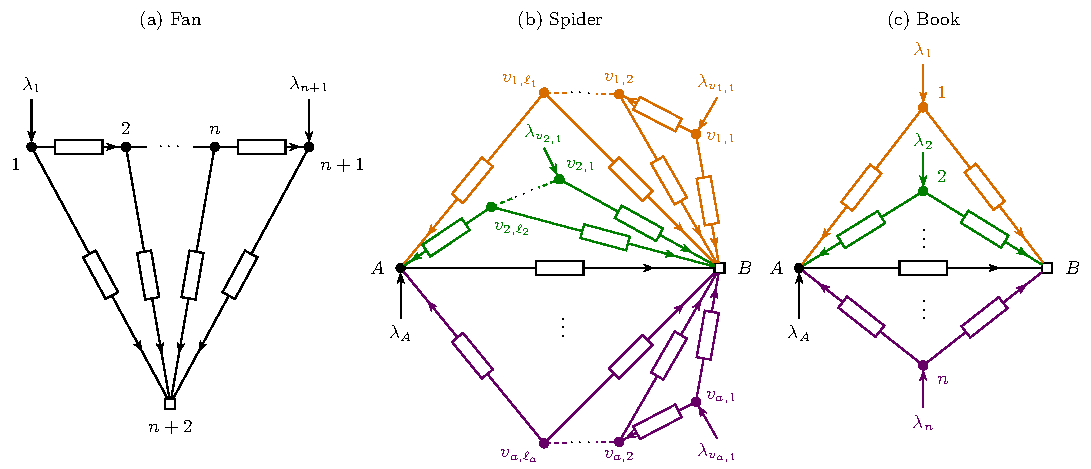
\includegraphics[width=\linewidth]{figures/circuits/sum_families.pdf}
\caption{(a) A \emph{fan}: the interaction vertices $1,\ldots,n+1$ form a path, and each of them is joined to the insertion $n+2$ by a spoke. (b) A \emph{spider}: several such paths, the arms, meet at a vertex $A$, and every vertex, $A$ included, is joined to a second vertex $B$; in $Q_n$, $A$ is the $\bar W$ vertex and $B=\mathcal O$. (c) A \emph{book}: a spider whose arms have one vertex each (Definition~\ref{def:spiders-books}).
}
\label{fig:sum-families}
\end{figure}
\item[(ii)] Every nonzero connected graph of the quantum product at order $\hbar^n$ consists of the marked edge $AB$ between the insertions and a forest of interaction trees $T_j$, each with at most one $\bar W$ vertex and joined to both insertions by $|T_j|+1$ spokes. For cubic interactions each tree carries exactly one source, at its unique vertex of degree two.
\begin{figure}[H]
\normalfont\centering
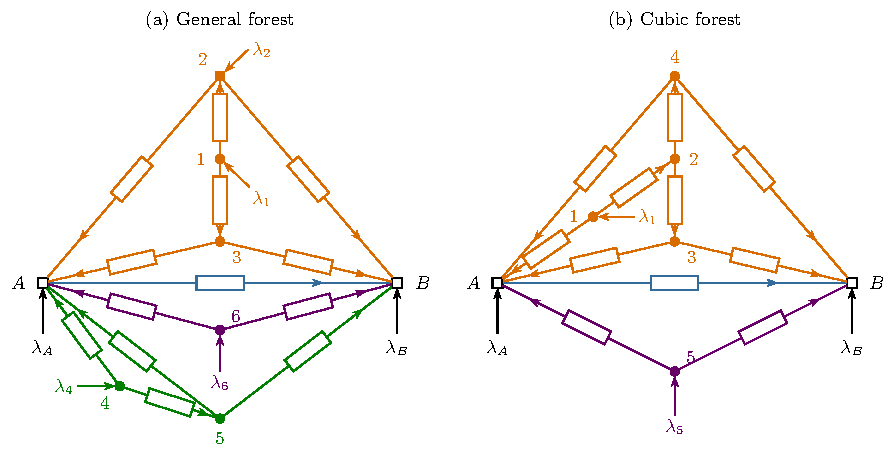
\includegraphics[width=.86\linewidth]{figures/circuits/sum_forests.pdf}
\caption{Graphs of the quantum product: the marked edge $AB$ (blue) between the insertions and a forest of interaction trees, each in its own colour and joined to $A$ and $B$ by one more spoke than it has vertices. (a) For general $\bar W$, each tree contains at most one $\bar W$ vertex (square). (b) For cubic interactions, each tree carries one source, at its vertex of degree two.
}
\label{fig:sum-forests}
\end{figure}
\end{enumerate}
\end{proposition}
Part~(i) combines Propositions~\ref{prop:cubicfan}, \ref{prop:cotangent-count} and~\ref{prop:superpotential-spider}; part~(ii) is Propositions~\ref{prop:product-forest} and~\ref{prop:product-cubic}. The same sections constrain the graphs further.

\begin{proposition}[Further constraints on the graphs]\label{prop:sum-constraints}
In the setting of Proposition~\ref{prop:sum-graphs}:
\begin{enumerate}
\item[(i)] Every nonzero graph of $Q_n$, and of the quantum product at order $\hbar^n$, has $n+2$ vertices and $2n+1$ edges, no self-loops and no parallel edges, and $|\Gamma_1[S]|\le2|S|-3$ for every vertex set $S$ with $|S|\ge2$.
\item[(ii)] A nonzero connected graph of $Q_n$, $n\ge1$, contains at most one $\bar W$ vertex, and each of its terms lowers the number of $\mathsf b,\beta$ factors by $n$ plus the number of $\bar W$ vertices.
\item[(iii)] In a nonzero graph of the quantum product, every interaction vertex has degree at least two, and loop diagrams contain no quadratic term of $\bar W$. A tree whose $\bar W$ vertex has $\deg_\Gamma\bar W$ contracted fields contains $\deg_\Gamma\bar W-2$ cubic vertices of degree two and keeps $\deg\bar W-2$ uncontracted fields.
\item[(iv)] For cubic interactions, the number of spokes at each vertex of a tree is fixed by its tree degree and by whether it is the vertex of degree two \eqref{eq:product-local-spokes}; conversely, the edge $AB$, a forest, and spokes obeying \eqref{eq:product-local-spokes}, with one vertex of degree two in each tree, form a graph satisfying (i).
\item[(v)] A graph of the quantum product is of type~I$'$ \cite[Definition 4.12]{GWW} if and only if the two endpoints of every internal edge are joined to a common insertion. Graphs of type~I$'$ are reduced to the edge $AB$ by series and parallel steps alone.
\end{enumerate}
\end{proposition}
These are \eqref{eq:1.12}--\eqref{eq:1.11}, Propositions~\ref{prop:cotangent-count}, \ref{prop:product-forest}, \ref{prop:product-cubic} and~\ref{prop:product-spider}, and \eqref{eq:1.23}.

Every graph above whose reduction needs no star--triangle move at a vertex carrying a source, in particular every graph of $Q_n$ and every graph of the quantum product for cubic interactions, is computed by one fixed routine that eliminates the interaction vertices one at a time (Section~\ref{sec:sum-reduction}). For the fan this gives the complete kernel in closed form at every $n$ (Theorem~\ref{thm:sum-kernels}(i)); for every other such graph, each term of every Taylor coefficient is a product of $O(n+m)$ factorials, linear in $n$ (Theorem~\ref{thm:sum-jets} and Table~\ref{tab:sum-costs}).

\subsection{Iterated reduction and closed kernels at every loop order}
\label{sec:sum-reduction}

One of our core observations is that the classical circuit moves can be iterated, transferring the sources at each step, as changes of variables on Schwinger space. Figure~\ref{fig:sum-moves} shows one step: a node $v$ with two neighbours $u,w$ is eliminated by a series step, and the parallel resistors $j=1,2,\ldots$ between $u$ and $w$ are merged.
\begin{figure}[H]
\centering
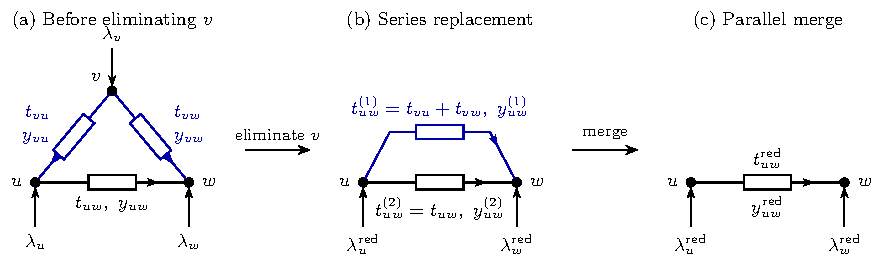
\includegraphics[width=.94\linewidth]{figures/circuits/sum_moves.pdf}
\caption{One elimination step. (a) The resistors $t_{vu},t_{vw}$ (blue) at the node $v$ are combined in series. (b) The source $\lambda_v$ is redistributed to $u$ and $w$, and the series resistor is in parallel with $t_{uw}$. (c) The parallel resistors are merged into one.}
\label{fig:sum-moves}
\end{figure}
\noindent The step \eqref{eq:1.64}, \eqref{eq:1.63} and its reversal, which writes the old currents as affine functions of the reduced ones, are
\begin{equation}\label{eq:sum-moves}
\begin{gathered}
r=\frac{t_{vu}}{t_{vu}+t_{vw}},\qquad t^{(1)}_{uw}=t_{vu}+t_{vw},\qquad
\lambda^{\mathrm{red}}_u=\lambda_u+(1-r)\lambda_v,\qquad
\lambda^{\mathrm{red}}_w=\lambda_w+r\lambda_v,\\
\frac1{t^{\mathrm{red}}_{uw}}=\sum_j\frac1{t^{(j)}_{uw}},\qquad r_j=\frac{t^{\mathrm{red}}_{uw}}{t^{(j)}_{uw}},\qquad\sum_jr_j=1,\\
y_{vu}=(1-r)\lambda_v-y^{(1)}_{uw},\qquad
y_{vw}=r\lambda_v+y^{(1)}_{uw},\qquad
y^{(j)}_{uw}=r_jy^{\mathrm{red}}_{uw},
\end{gathered}
\end{equation}
with the index $+\dot a$ suppressed. A trivalent node without source is removed by the star--triangle move \eqref{eq:1.62}.

\begin{theorem}[Kernels at every loop order]\label{thm:sum-kernels}
\begin{enumerate}
\item[(i)] For the $n$-loop fan with path $1-2-\cdots-(n+1)$, insertion $n+2$, sources $\lambda_1,\lambda_{n+1}$ at the endpoints of the path and displacements (holomorphic derivatives) $z_{i,n+2}=-z_i$ on the spokes, in the coordinates $r_1,\ldots,r_{2n}$ of \eqref{eq:1.36},
\begin{equation}\label{eq:sum-fan}
\begin{aligned}
&\mathcal I_\Gamma^{\mathrm{raw\ cut}}(\lambda;z)
\big|_{\lambda_2=\cdots=\lambda_n=0,
\ z_{i,i+1}=0,\ z_{i,n+2}=-z_i}\\
&=(\lambda_{1,+\dot a}\lambda_{n+1,+}{}^{\dot a})^n
\int d^{2n}r\,
\left[\prod_{j=1}^{n-1}r_{2j-1}^{n-j}r_{2j}(1-r_{2j})^{j-1}\right]
r_{2n}^{n-1}
e^{\sum_j y_{j,n+2,+\dot a}z_j^{+\dot a}},
\end{aligned}
\end{equation}
on $0<r_j<1$ $(j\le2n-2)$, $r_{2n-1},r_{2n}>0$, $r_{2n-1}+r_{2n}<1$. Reversing the reduction fixes the path currents backwards from $y_{n,n+1}$ and then the spoke currents by current conservation, all polynomial in $r$ \eqref{eq:1.38}, \eqref{eq:1.39}:
\begin{equation}\label{eq:sum-fan-currents}
\begin{gathered}
y_{n,n+1}=\Bigl(\prod_{k=1}^{n}r_{2k-1}\Bigr)\lambda_1-r_{2n}\lambda_{n+1},\\
y_{i,i+1}=r_{2i}\Bigl(\prod_{k=1}^{i}r_{2k-1}\Bigr)\lambda_1+(1-r_{2i})\,y_{i+1,i+2}\quad(1\le i<n),\\
y_{1,n+2}=\lambda_1-y_{12},\quad
y_{i,n+2}=y_{i-1,i}-y_{i,i+1}\ \ (2\le i\le n),\quad
y_{n+1,n+2}=\lambda_{n+1}+y_{n,n+1}.
\end{gathered}
\end{equation}
At zero displacement
\begin{equation}\label{eq:sum-fan-value}
\left.\mathcal I_\Gamma^{\mathrm{raw\ cut}}(\lambda;0)\right|_{\lambda_{2,+\dot a}=\cdots=\lambda_{n,+\dot a}=0}
=\frac{(\lambda_{1,+\dot a}\lambda_{n+1,+}{}^{\dot a})^n}{(n!)^3(n+1)}.
\end{equation}
\item[(ii)] For the spider with arms of lengths $\ell_1,\ldots,\ell_a$, $\sum_i\ell_i=n$, the vertices $v_{i,1},\ldots,v_{i,\ell_i}$ of arm $i$ labelled from its outer end towards $A$, and sources on the arms only at the outer ends, $\lambda_{v_{i,j}}=\delta_{j1}\lambda_{v_{i,1}}$ \eqref{eq:1.47},
\begin{equation}\label{eq:sum-spider}
\begin{aligned}
\mathcal I_\Gamma^{\mathrm{raw\ cut}}(\lambda;z)
={}&\int\prod_{i=1}^a\prod_{j=1}^{2\ell_i}dr_{i,j}\,
\left(1-\sum_i r_{i,2\ell_i}\right)
\prod_{i=1}^a\,
r_{i,2\ell_i}^{\ell_i-1}\prod_{j=1}^{\ell_i-1}\Big[r_{i,2j-1}^{\ell_i-j}\,r_{i,2j}^{\,j-1}\,(1-r_{i,2j})\Big]\\
&\times\bigl[\lambda_{v_{i,1},+\dot a}y^{\mathrm{red}}_{AB,+}{}^{\dot a}\bigr]^{\ell_i}
\,e^{-\sum_e y_{e,+\dot a}(r)z_e^{+\dot a}},
\end{aligned}
\end{equation}
on the domain and with the reduced current
\[
\begin{gathered}
0<r_{i,j}<1\ (j<2\ell_i),\qquad r_{i,2\ell_i}>0,\qquad \sum_ir_{i,2\ell_i}<1,\\
y^{\mathrm{red}}_{AB,+\dot a}=\lambda_{A,+\dot a}+\sum_i\Bigl(\prod_{k=1}^{\ell_i}r_{i,2k-1}\Bigr)\lambda_{v_{i,1},+\dot a}.
\end{gathered}
\]
Reversing the reduction of Figure~\ref{fig:sum-spider} on each arm, from $A$ outwards, gives the reduced spoke currents and then all currents, polynomial in $r$ \eqref{eq:spider-reconstruction-recurrence}, \eqref{eq:1.51}: with $v_{i,\ell_i+1}=A$ and $y^{\mathrm{red}}_{v_{i,\ell_i+1}B}=y^{\mathrm{red}}_{AB}$,
\begin{equation}\label{eq:sum-spider-currents}
\begin{gathered}
y^{\mathrm{red}}_{v_{i,j}B}=(1-r_{i,2j-1})\Bigl(\prod_{k=1}^{j-1}r_{i,2k-1}\Bigr)\lambda_{v_{i,1}}+r_{i,2j}\,y^{\mathrm{red}}_{v_{i,j+1}B}\quad(1\le j\le\ell_i),\\
y_{v_{i,j}v_{i,j+1}}=\Bigl(\prod_{k=1}^{j-1}r_{i,2k-1}\Bigr)\lambda_{v_{i,1}}-y^{\mathrm{red}}_{v_{i,j}B},\qquad
y_{v_{i,1}B}=y^{\mathrm{red}}_{v_{i,1}B},\\
y_{v_{i,j}B}=(1-r_{i,2j-2})\,y^{\mathrm{red}}_{v_{i,j}B}\quad(j\ge2),\qquad
y_{AB}=\Bigl(1-\sum_ir_{i,2\ell_i}\Bigr)y^{\mathrm{red}}_{AB}.
\end{gathered}
\end{equation}
\item[(iii)] For the book with pages $1,\ldots,n$, $A=n+1$, $B=n+2$, a source on every page and the currents \eqref{eq:B-book-reduced-current},
\begin{equation}\label{eq:sum-book}
\begin{aligned}
\mathcal I_\Gamma^{\mathrm{raw\ cut}}(\lambda;z)
={}&\int_{\substack{0<r_{2i-1}<1\\r_{2i}>0,\ \sum_ir_{2i}<1}}
 dr_1\cdots dr_{2n}\,
 \Bigl(1-\sum_{i=1}^nr_{2i}\Bigr)\\
&\times\prod_{i=1}^n\Bigl[
\lambda_{i,+\dot a_i}\Bigl(\lambda_{n+1,+}{}^{\dot a_i}
+\sum_{j=1}^nr_{2j-1}\lambda_{j,+}{}^{\dot a_i}\Bigr)\Bigr]
e^{-\sum_{e}y_{e,+\dot a}z_e^{+\dot a}}.
\end{aligned}
\end{equation}
\item[(iv)] Every product forest with cubic vertices is reduced to one resistor by star--triangle moves at its source-free trivalent nodes, series steps and parallel merges (Figure~\ref{fig:sum-forest}). In the reversed coordinates its currents and its density are polynomial, and every coefficient is a finite sum of the Dirichlet moments \eqref{eq:Dirichlet}.
\end{enumerate}
In (i)--(iii) the complete Taylor expansions in the displacements of all edges are the explicit finite factorial sums \eqref{eq:fan-full-taylor} and \eqref{eq:spider-full-taylor}.
\end{theorem}
The proofs are in Sections~\ref{sec:fans} and~\ref{sec:forests} and Appendix~\ref{sec:network}.\footnote{For $n=1,2,3$, \eqref{eq:sum-fan-value} agrees with the operatope values \cite[Equations (4.20), (4.44), (4.67)]{operatope} and with the fans of Gui, Wang and Williams \cite[Sections 4.4--4.6]{GWW}; at $n=1$ it is the coefficient of \cite[Equation (2.48)]{BK}.}

\begin{figure}[H]
\centering
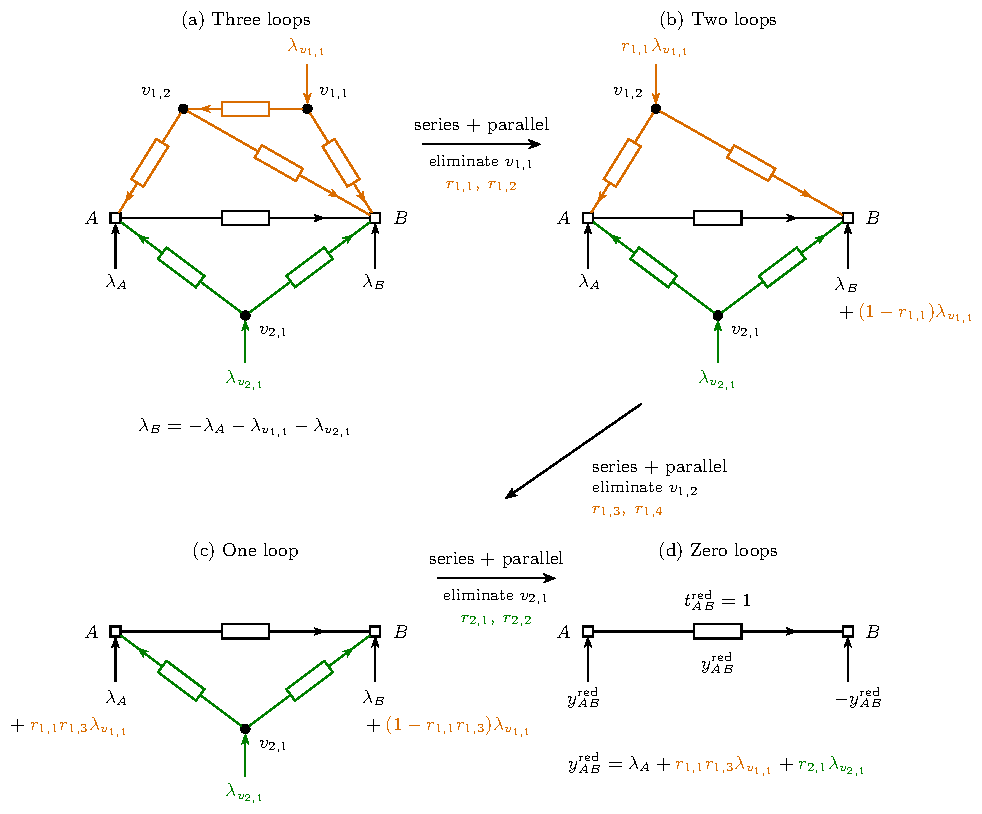
\includegraphics[width=.86\linewidth]{figures/circuits/spider_reduction.pdf}
\caption{Iterated reduction of the three-loop spider with arms $\ell_1=2$ and $\ell_2=1$ (Section~\ref{sec:spiders}); for $Q_n$, $A$ is the $\bar W$ vertex and $B=\mathcal O$. Each step eliminates an arm vertex by a series step, which passes the fraction $r_{i,2j-1}$ of its source along the arm and the rest to $B$, and a parallel merge; each step lowers the loop number by one, down to the unit resistor carrying $y^{\mathrm{red}}_{AB}$.}
\label{fig:sum-spider}
\end{figure}

\begin{figure}[H]
\centering
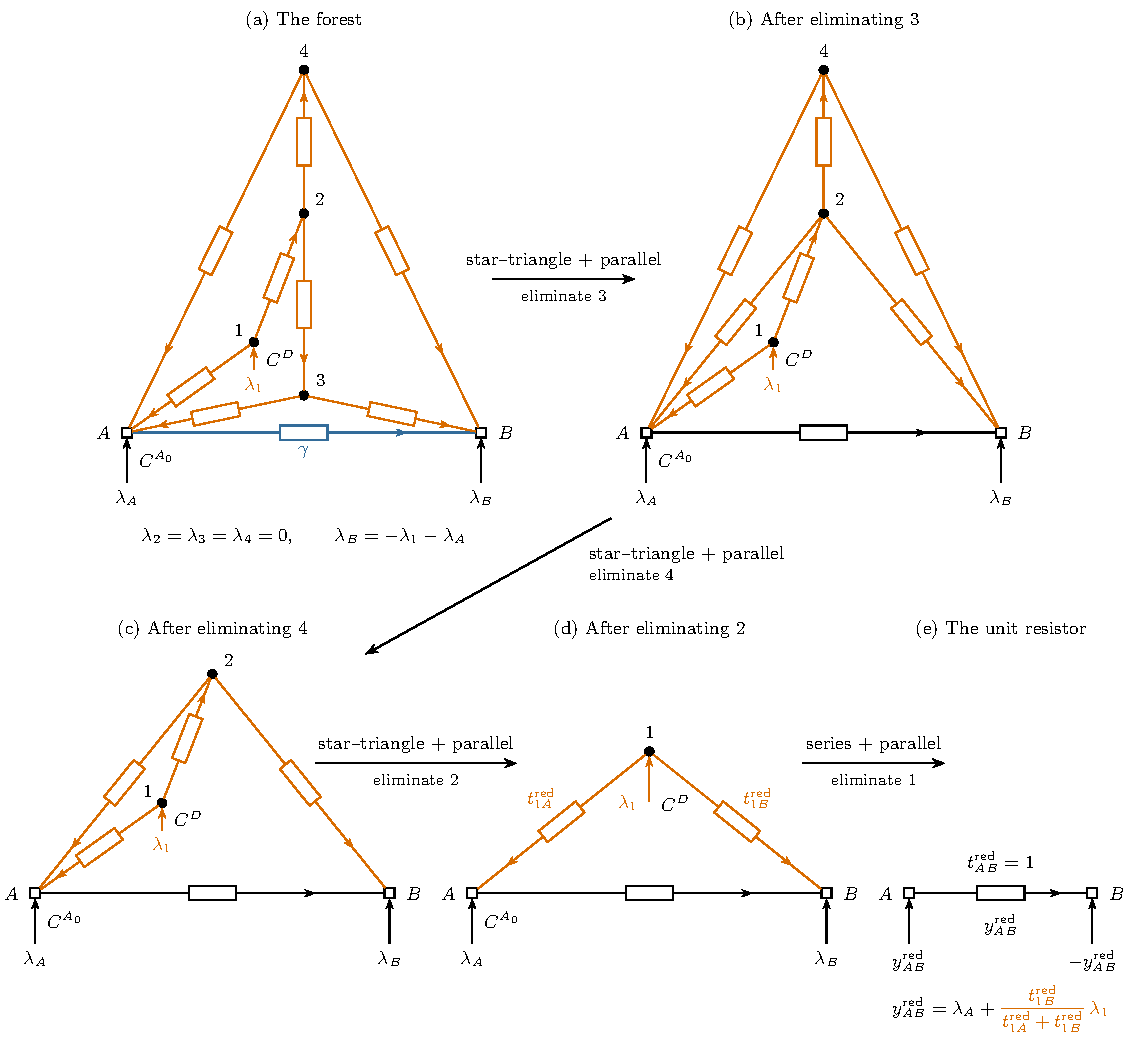
\includegraphics[width=\linewidth,height=.62\textheight,keepaspectratio]{figures/circuits/forest_star_triangle_v3.pdf}
\caption{Reduction of a four-loop product forest with tree edges $12,23,24$, spokes $1A,3A,3B,4A,4B$ and the marked edge $AB$ in blue (Section~\ref{sec:forest-graphs}). Star--triangle moves remove the source-free vertices $3$, $4$ and $2$, one per step, and the new resistors merge in parallel with existing ones; the root $1$, carrying $\lambda_1$, is removed last by a series step and a parallel merge with $AB$.
}
\label{fig:sum-forest}
\end{figure}

\subsection{Cost of exact coefficients}

In Schwinger times each current is a ratio of sums over spanning trees, and their number grows exponentially with the loop order. In the circuit coordinates of graphs reduced without star--triangle moves at nodes carrying sources the density has no denominator (Table~\ref{tab:sum-costs}). Below, $m$ is the total degree in the displacements (holomorphic derivatives).

\begin{table}[H]
\centering\small
\caption{One exact coefficient of the kernel at $n$ loops. In the original method the Schwinger-time integrand has as denominator a power of the tree polynomial $\sum_T\prod_{h\notin T}t_h$, which has one monomial per spanning tree \cite[Corollaries 1--2]{Wang}, \eqref{eq:forestuniform}; $F_k$ is the $k$th Fibonacci number.}
\label{tab:sum-costs}
\begin{tabular}{>{\raggedright\arraybackslash}p{.22\linewidth}>{\raggedright\arraybackslash}p{.22\linewidth}>{\raggedright\arraybackslash}p{.46\linewidth}}
\toprule
Graphs&Spanning trees (original method)&Circuit coordinates\\
\midrule
fan, $n$ loops&$F_{2n+2}\sim2.62^n$&monomial density \eqref{eq:sum-fan}, closed value \eqref{eq:sum-fan-value}; $O(n(m+1)^2)$ operations per jet coefficient, linear in $n$\\[3pt]
spider, arms $\ell_1,\ldots,\ell_a$&between book and fan&density \eqref{eq:sum-spider}; $O(n+m)$ operations per term of \eqref{eq:spider-full-taylor}\\[3pt]
book, $n$ pages&$2^{n-1}(n+2)$&density \eqref{eq:sum-book}; $O(n+m)$ operations per term\\[3pt]
type I$'$ product forests&exponential&spider density with the reduced current \eqref{eq:product-typeI-current}; $O(n+m)$ operations per term\\[3pt]
cubic product forests not of type I$'$&exponential&polynomial density; $O(n+m)$ operations per Dirichlet moment \eqref{eq:Dirichlet}\\[3pt]
sourced trivalent nodes&exponential&rational currents; convergent series \eqref{eq:1.81}\\
\bottomrule
\end{tabular}
\end{table}

\begin{theorem}[Exact jets in polynomial time]\label{thm:sum-jets}
Let the interaction be \eqref{eq:B.10}, with the superpotential $\bar W$ a polynomial or, coefficientwise, a formal power series of $\bar\phi$ and $\bar W_{\dot a}$. For a graph of $Q_n$, a jet coefficient of order $m$ is the coefficient, in \eqref{eq:fan-full-taylor} or \eqref{eq:spider-full-taylor}, of one monomial in the source--source and source--displacement pairings, treated as independent symbols, of total degree $m$ in the displacements (holomorphic derivatives).
\begin{enumerate}
\item[(i)] For every $n\ge1$ and every graph of $Q_n$, every jet coefficient is a rational number, a finite sum of terms, each a product of $O(n+m)$ factorials and ratios of factorials of integers at most $n+m+2$.
\item[(ii)] For an $n$-loop fan put $N_\Gamma=\tfrac12n(n+1)+n+2$ and $T_\Gamma=1$; for a spider with arms $\ell_1,\ldots,\ell_a$ put $N_\Gamma=\sum_i\tfrac12\ell_i(\ell_i+1)+(n+1)(a+1)$ and $T_\Gamma=\prod_{i=1}^a\binom{\ell_i+a-1}{a-1}$. All jet coefficients of order at most $m$ are obtained exactly with $O\bigl((n+m)\,T_\Gamma\binom{m+N_\Gamma}{N_\Gamma}\bigr)$ arithmetic operations. This is polynomial in $m$ at fixed $n$, and polynomial in $n$ at fixed $m$ and $a$. For $\bar W$ of fixed degree, and in every theory with cubic interactions, the graphs of $Q_n$ are the fan and at most $\sum_{a<\deg\bar W}\binom{n-1}{a-1}$ spiders, so at fixed $m$ all jets of order at most $m$ of all kernels of $Q_n$ are computed in time polynomial in $n$.
\item[(iii)] For the $n$-loop fan with sources at the endpoints of the path, each jet coefficient of order $m$ costs $O(n(m+1)^2)$ operations, linear in $n$, so all coefficients of order at most $m$ are computed with $O\bigl(n(m+1)^2\binom{m+2n+2}{2n+2}\bigr)$ operations, polynomial in $n$, $m$ and their number.
\item[(iv)] For cubic interactions and each graph of the quantum product, the Taylor coefficients of order at most $m$ in the displacements (holomorphic derivatives) are polynomials in the sources with rational coefficients, obtained in time polynomial in $m$.
\end{enumerate}
\end{theorem}
The proof is in Appendix~\ref{sec:B-jets}; part~(iii) rests on a nested Beta recursion, Lemma~\ref{lem:fan-recursion}.\footnote{The same iterated reduction computes the analogous current integrals on $\mathbb C^d$ over networks that series, parallel and source-free star--triangle moves reduce to one resistor (Appendix~\ref{sec:B-jets}).}

\subsection{The all-order supercharge of \texorpdfstring{$\mathcal N=4$}{N=4} Yang--Mills theory}

Since only fans occur, \eqref{eq:sum-fan} gives the supercharge of $\mathcal N=4$ Yang--Mills theory at every loop order in closed form: the functional derivatives act at $x+z_j$, and the two output superfields are evaluated at $x+x_1(r,z)$ and $x+x_{n+1}(r,z)$, convex combinations of the $z_j$ with coefficients polynomial in $r$.

\begin{theorem}[All-loop supercharge of $\mathcal N=4$ Yang--Mills theory]\label{thm:sum-N4}
For the superfield action \eqref{eq:A.15} and an operator at $x$, the $n$-loop supercharge for $n\ge1$ is
\begin{equation}\label{eq:sum-N4}
\begin{aligned}
Q_n={}&\frac{(-1)^ni^{n+1}}{2(32\pi^2)^n}
\int_{\eqref{eq:1.37}}dr_1\cdots dr_{2n}\,
\left[\prod_{j=1}^{n-1}r_{2j-1}^{n-j}r_{2j}(1-r_{2j})^{j-1}\right]r_{2n}^{n-1}
\int d^3\theta\int\prod_{j=1}^{n+1}d^4z_j\\
&\times C_{A_1DR_1}
\left(\prod_{j=2}^{n}C_{A_jR_{j-1}R_j}\right)C_{A_{n+1}R_nE}\\
&\times\big(\partial_{+\dot a_1}\cdots\partial_{+\dot a_n}C^D\big)(x+x_1(r,z),\theta)
\big(\partial_+{}^{\dot a_1}\cdots\partial_+{}^{\dot a_n}C^E\big)(x+x_{n+1}(r,z),\theta)\\
&\times\frac{\delta}{\delta C^{A_1}(x+z_1,\theta)}\cdots
\frac{\delta}{\delta C^{A_{n+1}}(x+z_{n+1},\theta)},
\end{aligned}
\end{equation}
where the output fields are differentiated before they are evaluated at the translated positions
\begin{equation}\label{eq:sum-N4-points}
\begin{aligned}
x_1^{+\dot a}(r,z)
={}&\sum_{j=1}^{n}(1-r_{2j-1})
\left(\prod_{k=1}^{j-1}r_{2k-1}\right)
\left[
\left(\prod_{k=1}^{j-1}(1-r_{2k})\right)z_1^{+\dot a}
+\sum_{i=2}^{j}r_{2i-2}
\left(\prod_{k=i}^{j-1}(1-r_{2k})\right)z_i^{+\dot a}
\right]\\
&+\left(\prod_{k=1}^{n}r_{2k-1}\right)z_{n+1}^{+\dot a},\\
x_{n+1}^{+\dot a}(r,z)
={}&r_{2n}\left[
\left(\prod_{k=1}^{n-1}(1-r_{2k})\right)z_1^{+\dot a}
+\sum_{i=2}^{n}r_{2i-2}
\left(\prod_{k=i}^{n-1}(1-r_{2k})\right)z_i^{+\dot a}
\right]
+(1-r_{2n})z_{n+1}^{+\dot a}.
\end{aligned}
\end{equation}
\end{theorem}
This is Theorem~\ref{thm:N4-allloop} with \eqref{eq:fan-output-points}. Each $r_j$ is a parallel current-division ratio (Figure~\ref{fig:sum-moves}): for $i<n$, $r_{2i-1}$ is the fraction of the source at $i$ passed to $i+1$ and $r_{2i}$ the fraction of the merged spoke current carried by the original spoke $(i+1,n+2)$, and in the final triangle $r_{2n-1}$ and $r_{2n}$ are the fractions of the sources at $n$ and $n+1$ that flow through the edge $(n,n+1)$. $Q_n$ replaces $n+1$ input letters by two output letters.\footnote{At one loop, $Q_1$ agrees with the operator of Budzik and Kulp \cite[Equations (3.64)--(3.70)]{BK} up to normalization; its component \eqref{eq:2.26} is the Konishi anomaly.}

\begin{lemma}[Derivative grading]\label{lem:sum-grading}
A monomial has two holomorphic derivative totals, its numbers of $\partial_{+\dot+}$ and $\partial_{+\dot-}$ derivatives. A class can be $d_r$-exact, for the successive differential $d_r$ of Section~\ref{sec:homotopy-transfer}, only if both derivative totals of its leading representative are at least $r$. In particular, a class whose leading representative has no holomorphic derivatives is $d_r$-exact for no $r\ge1$.
\end{lemma}
This is Lemma~\ref{lem:derivative-grading}.

\begin{theorem}[Finite loop order]\label{thm:sum-finite}
For the interaction \eqref{eq:B.10} with $\bar W$ of any degree, and every monomial $\mathcal O$,
\begin{equation}\label{eq:sum-finite}
Q_n\mathcal O=0\qquad\text{for }n>\#(\mathsf b,\beta\text{ in }\mathcal O).
\end{equation}
\end{theorem}
This is Corollary~\ref{cor:finite-loop}.

If the interaction satisfies the quantum master equation $\sum_{n\ge0}\frac{\hbar^n}{n+2}Q_n\mathcal I=0$ \eqref{eq:2.40}, then $\mathbf Q^2=0$ (Lemma~\ref{lem:qme-nilpotence}). For the holomorphic twist of an off-shell $\mathcal N=1$ gauge theory, renormalizable or not, with gauge-invariant $\bar W$ and
$\operatorname{Tr}_R(t_A\{t_B,t_C\})=0$,
\begin{equation}\label{eq:sum-QI}
Q_0\mathcal I=0,\qquad Q_1\mathcal I=\frac{ig^3}{128\pi^2}
\operatorname{Tr}_R\!\left(t_A\{t_B,t_C\}\right)
\mathsf c^A(\partial_{+\dot a}\mathsf c^B)
(\partial_+{}^{\dot a}\mathsf c^C)=0,\qquad
Q_{n\ge2}\mathcal I=0,
\end{equation}
so \eqref{eq:2.40} holds (Theorem~\ref{thm:interaction-consistency}).

\subsection{The quantum product and the quantum BPS ring}

From one loop on, $\mathbf Q$ violates the Leibniz rule for the ordinary product of local operators. The quantum product, the marked operation of Gaiotto, Kulp and Wu \cite[Sections 4.3 and 4.5]{higher},
\begin{equation}\label{eq:sum-star}
A\star B=\sum_{n\ge0}\frac{\hbar^n}{n!}
\{\mathcal I^{\otimes n},A,B\}^{\gamma,0},
\end{equation}
where $\gamma=\{(A,B)\}$ marks the edge $AB$ between the insertions, contracted last with $z_{AB}=0$ \eqref{eq:1.3}, repairs it. For quantum cocycles $A=\sum_i\hbar^iA_i$ and $B=\sum_j\hbar^jB_j$ its coefficients
$\mathcal O_r=\sum_{i+j+n=r}\frac1{n!}\{\mathcal I^{\otimes n},A_i,B_j\}^{\gamma,0}$, $\mathcal O_0=A_0B_0$, satisfy $\sum_{k=0}^rQ_k\mathcal O_{r-k}=0$ at every order \eqref{eq:2.32}: the product gives in closed form a completion of $A_0B_0$. Its order-$\hbar^n$ term needs at least $n$ factors of $\mathsf b$ or $\beta$ from its two inputs, so it is finite on local operators of finite length and derivative order.

\begin{theorem}[Quantum BPS ring]\label{thm:sum-ring}
Suppose that the interaction satisfies \eqref{eq:2.40} and, for (ii) and (iii), that the marked higher operations satisfy their quadratic identities.
\begin{enumerate}
\item[(i)] $\mathbf Q(A\star B)=(\mathbf QA)\star B+(-1)^{|A|}A\star(\mathbf QB)$, with $|A|$ the fermion number of $A$.
\item[(ii)] The quantum product induces an associative, graded-commutative, unital multiplication on $H(\mathbf Q)$.
\item[(iii)] On the pages $E_1=H(Q_0)$, $E_{r+1}=H(E_r,d_r)$ of the successive homotopy transfer (Section~\ref{sec:homotopy-transfer}), it induces the ordinary product of the $\hbar^0$ terms of representatives, and every differential $d_r$ is a derivation of it.
\item[(iv)] For homogeneous quantum cocycles $A,B$ and every $L>0$, $A\star B$ is cohomologous, in the effective-observable complex at scale $L$, to the quantum normal-ordering product of \cite[Section 2.3]{semichiral}, the contour integral \eqref{eq:ring-normal-ordering} of the scale-$L$ two-insertion expansion of $A$ around $B$.
\end{enumerate}
\end{theorem}
These are Theorems~\ref{thm:leibniz}, \ref{thm:quantum-bps-ring} and~\ref{thm:normal-ordering}.\footnote{The quantum product is the marked operation of Gaiotto, Kulp and Wu \cite[Sections 4.3 and 4.5]{higher}. Part~(i) follows from the quadratic identities of the higher brackets \cite[Section 3.2]{operatope}, \cite[Theorem 7]{Wang}, \cite[Equations (4.19), (4.42)]{higher} with one marked edge; the Leibniz rule and a ring structure for the quantum normal-ordering product were anticipated in \cite[Section 2.2 and footnote 28]{semichiral}, and the two-mark associator graph is drawn in \cite[Figure 7]{higher}. The all-order associativity homotopy behind (ii), the strict unit, the page statement (iii), the identification (iv) at every order, and the circuit proof of the quadratic identities (Appendix~\ref{sec:B-short-circuits}) are derived here. The theorem assembles these into one statement, and the kernels of Section~\ref{sec:sum-reduction} evaluate the product graph by graph. To our knowledge, the four statements have not been formulated together before.} In $\mathcal N=4$ Yang--Mills theory, with the vertices $1:\mathcal I$, $2:A$, $3:B$ and the marked edge $(2,3)$, the one-loop product is
\begin{equation}\label{eq:sum-product1}
\begin{aligned}
\{\mathcal I,A,B\}^{\{(2,3)\},0}
={}&\frac{i}{32\pi^2}\int_0^1dr_1\int_0^{1-r_1}dr_2
\int d^3\theta\,C_{XYZ}\int d^4z_1\,d^4z_2\\
&\times(\partial_{+\dot a}C^X)\big(r_1z_1+(1-r_1)z_2,\theta\big)\\
&\times\left.
\partial_{2,+}{}^{\dot a}
\left(\frac{\delta A(x_2)}{\delta C^Y(x_2+z_1,\theta)}\right)
\right|_{x_2=r_2(z_2-z_1)}
\frac{\delta B(0)}{\delta C^Z(z_2,\theta)},
\end{aligned}
\end{equation}
where $\partial_{2,+}{}^{\dot a}$ differentiates the surviving fields of $A$ at fixed $z_1$ before the displayed position is substituted \eqref{eq:2.34}.\footnote{The product is associative only up to exact terms. With flavour indices $2,3$, the matrix notation of Section~\ref{sec:graviton-closure} and $\operatorname{Tr}(\gamma^2\gamma^2)=\delta^{XY}(\gamma^2)_X(\gamma^2)_Y$, exactly
\[
\begin{aligned}
&\bigl(\operatorname{Tr}(\gamma^2\gamma^2)\star\operatorname{Tr}(\gamma^2\gamma^2)\bigr)\star\operatorname{Tr}(\gamma^3\beta_2)
-\operatorname{Tr}(\gamma^2\gamma^2)\star\bigl(\operatorname{Tr}(\gamma^2\gamma^2)\star\operatorname{Tr}(\gamma^3\beta_2)\bigr)\\
&\quad=-\frac{i\hbar g}{16\pi^2}\operatorname{Tr}\bigl((\partial_{+\dot a}\mathsf c)[\gamma^2,\gamma^3]\bigr)\,\partial_+{}^{\dot a}\operatorname{Tr}(\gamma^2\gamma^2)
=\mathbf Q\Big[\frac{\hbar}{16\pi^2}\bigl(\partial_{+\dot a}\operatorname{Tr}(\gamma^2\gamma^2)\bigr)\operatorname{Tr}\bigl((\partial_+{}^{\dot a}\gamma^2)\gamma^3\bigr)\Big]
\end{aligned}
\]
(Example~\ref{prop:scalar-associator}).} Section~\ref{sec:product-loops} gives the complete two-loop product, whose graphs are a book and two fans. At every order the books and spiders among the product graphs have the kernels of Theorem~\ref{thm:sum-kernels}(ii)--(iii); the other graphs, which first occur at three loops, are the cubic forests of Theorem~\ref{thm:sum-kernels}(iv).

\paragraph{Uses of the quantum product.} The quantum product gives closed completions, which the naive classical (Wick) product does not.
\begin{enumerate}
\item[(a)] \emph{Multi-gravitons remain quantum cocycles.} In $\mathcal N=4$ Yang--Mills theory the single gravitons, the components $G$ of $\operatorname{Tr}(dC)^p$ \cite[Section 4]{ChangYin}, satisfy $Q_nG=0$ for every $n$ \eqref{eq:2.60}: the fan kernel contains $\prod_{j=1}^n\prod_{I=1}^3(\theta_I^{(j)}-\theta_I^{(j+1)})$, which needs $3n$ odd derivatives, while the $n+1$ contracted factors of $dC$ supply at most $n+1$, so every single graviton is a quantum cocycle; at one loop this is \cite[Section 3.4.1]{BK}. The quantum product guarantees that multi-gravitons are quantum cocycles as well: every iterated quantum product $\mathcal O$ of single gravitons $G_1,\ldots,G_m$, with any bracketing, satisfies
\begin{equation}\label{eq:sum-multigraviton}
\mathbf Q\mathcal O=0,\qquad
\left.\mathcal O\right|_{\hbar=0}=G_1\cdots G_m,
\end{equation}
and each fixed component has finitely many corrections: with $\deg_\theta$ equal to $0,1,2,3$ on $\mathsf c,\gamma,\beta,\mathsf b$ \eqref{eq:2.62}, the coefficient of $\hbar^n$ vanishes once $3n>\deg_\theta(G_1\cdots G_m)$ (Theorem~\ref{thm:multigraviton-closure}).
\item[(b)] \emph{Dressed classes are completed by one more product.} Once a class $\mathcal O_0$ has a closed completion $\mathcal O[\mathcal O_0]$, every graviton-dressed class $G\mathcal O_0$ is completed by $G\star\mathcal O[\mathcal O_0]$, with no new obstruction calculation: once $\mathcal O_0$ has a closed completion, the dressed class needs no closure test of its own.
\item[(c)] \emph{Higher differentials vanish on completed classes.} A class with a closed completion is annihilated by every $d_r$ \eqref{eq:graviton-dr-zero}.\footnote{We remind the reader that such a class is a quantum cocycle, lifted exactly when it becomes a quantum coboundary: it survives unless it is $d_r$-exact for some $r\ge0$, and a leading representative without holomorphic derivatives is $d_r$-exact for no $r\ge1$ (Lemma~\ref{lem:sum-grading}). A closed multi-graviton can still be the exact member of a lifted pair, as in the one-loop $SO(7)$ example of \cite[Section 3]{KonishiBH}, and no differential maps one graviton class to another.} In $\mathcal N=4$ Yang--Mills theory with gauge group of finite rank, in each charge sector and cohomological degree $k$,
\begin{equation}\label{eq:sum-rank}
\sum_{r\ge1}\operatorname{rank}d_r^k\le\#\{\text{fortuitous classes of degree }k\},
\end{equation}
and fortuitous classes are sparse among the classical classes known so far \cite{microstates,KKLP}.
\item[(d)] \emph{The ring is explicit.} Theorem~\ref{thm:sum-ring} gives the multiplication on $H(\mathbf Q)$, the perturbative quantum BPS ring of $\mathcal N=4$ Yang--Mills theory, and \eqref{eq:sum-star} computes it graph by graph.
\item[(e)] \emph{Closure tests reduce to generators.} Since every $d_r$ is a derivation of the product on $E_r$ \eqref{eq:2.78}, it is fixed by its values on algebra generators of $E_r$; on products of single gravitons every $d_r$ vanishes by (a) and (c), and on a product of classes on $E_r$ it is fixed by its values on the factors. For the classes known so far, mostly multi-gravitons, this reduction is immediate; it applies unchanged once fortuitous generators are included.
\end{enumerate}

\subsection{Loop obstructions and lifting beyond one loop}

From the second page on, $d_r$ is not the class of $Q_r$: for a class surviving one loop, with $Q_0\mathcal O_1=-Q_1\mathcal O_0$,
\begin{equation}\label{eq:sum-d2}
Q_0Q_2\mathcal O_0=Q_1Q_0\mathcal O_1,\qquad
d_2[\mathcal O_0]_2=[Q_2\mathcal O_0+Q_1\mathcal O_1]_2,
\end{equation}
and $d_2[\mathcal O_0]_2=0$ if and only if $Q_2\mathcal O_0+Q_1\mathcal O_1\in\operatorname{im}Q_0+Q_1\ker Q_0$, with $\ker Q_0$ in the first-correction sector \eqref{eq:d2-quotient-test}.\footnote{Algorithmically, a rational linear functional that vanishes on $\operatorname{im}Q_0+Q_1\ker Q_0$ but not on $Q_2\mathcal O_0+Q_1\mathcal O_1$ certifies $d_2[\mathcal O_0]_2\ne0$.} A cocycle survives at every perturbative order if it admits a closed completion and is $d_r$-exact for no $r\ge0$, where $d_0=Q_0$ (Section~\ref{sec:homotopy-transfer}). Our algorithm for these tests is given in Appendix~\ref{sec:algorithm}.

\paragraph{Two-loop lifting.} In massive supersymmetric electrodynamics with
\begin{equation}\label{eq:sum-SQED}
\mathcal I=ig\mathsf c(\gamma_+\beta^+-\gamma_-\beta^-)+\frac m2\gamma_s^2+y\gamma_s\gamma_+\gamma_-,\qquad gmy\ne0,
\end{equation}
the cocycle
\begin{equation}\label{eq:sum-SQEDsource}
\mathcal O_0=ig\Big[\beta^+\beta^-\mathsf b^2
+\frac ym(\gamma_-\beta^--\gamma_+\beta^+)\beta^s\mathsf b^2
+\frac{y^2}{3m\,ig}\gamma_+\gamma_-\mathsf b^3\Big]
\partial_{+\dot a}\mathsf c
\end{equation}
has a one-loop completion, is not $d_1$-exact by its derivative totals $(1,0)$ (Lemma~\ref{lem:sum-grading}), and is lifted at two loops:
\begin{equation}\label{eq:sum-SQEDlift}
d_2[\mathcal O_0]_2
=-\frac{2(ig)^2y^4}{m^2(64\pi^2)^2}\Big[
\partial_{+\dot a}(\gamma_+\gamma_-)
\,\partial_{+\dot b}\partial_{+\dot c}(\gamma_+\gamma_-)
\,\partial_+{}^{\dot b}\partial_+{}^{\dot c}(\gamma_+\gamma_-)
\Big]_2\ne0.
\end{equation}
To our knowledge this is the first example of two-loop lifting (Section~\ref{sec:SQEDlift}); it answers, for this theory, the question left open in \cite[Section 1]{BK}, although, somewhat disappointingly, none of the fortuitous classes tested here is lifted beyond one loop: each survives at every perturbative order.

\paragraph{Protected classes in \texorpdfstring{$\mathcal N=4$}{N=4} Yang--Mills theory.} Every $\mathcal N=4$ class tested here survives at every perturbative order (Section~\ref{sec:applications}).
\begin{itemize}
\item The $18$ multi-graviton classes of the four-letter $SU(2)$ sector of Section~\ref{sec:finite-sectors} have closed completions ending at order $\hbar$, and the $9$ classes of the five-letter $SU(3)$ sector of flavour weight $(3,3,2)$ closed completions ending at order $\hbar^2$; for the class \eqref{eq:su3-example-source}, $Q_2\mathcal O_0=0$ but $Q_1\mathcal O_1=-Q_0\mathcal O_2\ne0$.
\item The threshold fortuitous class of $SU(2)$ \cite[Section 3.1]{KKLP} has the closed completion $\sum_{r=0}^4\hbar^r\mathcal O_r$ \eqref{eq:threshold-completion}: each order removes one letter and three units of $\deg_\theta$ and adds two holomorphic derivatives, from $7$ letters at $r=0$ to $3$ letters with $8$ derivatives at $r=4$, and $\mathcal O_4$ has the coefficients $-42731/432$, $23323/216$ and $90043/432$ times $(ig)^3/(32\pi^2)^4$ \eqref{eq:threshold-fourth}. Although $Q_2\mathcal O_0\ne0$, $d_2[\mathcal O_0]_2=0$. The leading term has no holomorphic derivatives, so the class is $d_r$-exact for no $r\ge1$ (Lemma~\ref{lem:sum-grading}) and survives at every perturbative order, as argued from charge counting in \cite[Section 3]{ChangLin}.
\item The three graviton-hair classes of the threshold class \cite[Section 3.2]{KKLP} are completed by $(w_2)^I\star\mathcal O[\mathcal O_0]$, with the two-letter single graviton $(w_2)^I$ of \eqref{eq:w2}, by its descendant $\varepsilon_{IJK}Q_+^IQ_+^J\bigl((w_2)^K\star\mathcal O[\mathcal O_0]\bigr)$, and by the quantum product of the graviton factor of \eqref{eq:hair-derivative} with $\mathcal O[\mathcal O_0]$; with an explicit check that the last is not $d_1$-exact, all three survive at every order.
\end{itemize}

\paragraph{Quartic deformation.} In the $SU(2)$ theory with $\bar W=-\frac1{2M}\operatorname{Tr}[\gamma^1,\gamma^2]^2$, $M\ne0$, obtained from $\mathcal N=4$ Yang--Mills theory by a mass for one adjoint chiral multiplet, the supercharge contains spider kernels. The square $w^2$ of the graviton $w$ \eqref{eq:quartic-square} of \cite{CK} has a closed completion ending at order $\hbar^3$, with $Q_2\mathcal O_1=0$ and $Q_3\mathcal O_0$, $Q_1\mathcal O_2$, $Q_0\mathcal O_3$ proportional to one operator with coefficients $-16$, $-42$, $58$; the non-graviton class $\mathcal O_{16}$ of \cite{CK} has a closed completion ending at order $\hbar^4$. Both survive at every perturbative order (Section~\ref{sec:quartic-fortuitous}).

\section{Holomorphic observables and graph operations}
\label{sec:setup}

We use the holomorphic Feynman graph integrals of \cite{Wang,operatope}, the higher operations of \cite{higher} and the holomorphic supercharge construction of \cite[Equation (3.33)]{semichiral} and \cite{BK}.\footnote{For the foundation of the holomorphic twist, see Appendix~\ref{sec:BV}: adding $Q_-$ to the BRST differential and performing a homotopy transfer derives the holomorphically twisted theory from the original physical theory.} Appendix~\ref{sec:quantum-transfer} derives the formula by heat-kernel transfer in Costello's formalism \cite{Costello}, relying on the ultraviolet finiteness of the holomorphically twisted theory \cite[Corollary 4]{Wang}, and explains its interpretation in the quantum BV complex; Appendix~\ref{sec:feynman-rules} collects the Feynman rules.

\begin{definition}[Brackets and the full quantum differential]\label{def:brackets}
Let $\mathcal O_1,\ldots,\mathcal O_k$ be homogeneous operators of fermion numbers $|\mathcal O_i|$, with $\mathcal O_k$ at the origin. Let $\Gamma$ run over connected contraction graphs, with edges $\Gamma_1=(e_1,\ldots,e_{|\Gamma_1|})$ in their contraction order; write $\Omega_v$ for the holomorphic volume form at vertex $v$, $[P_{\varepsilon,L;e}]_\Omega$ and $[K_{\varepsilon;e}]_\Omega$ for the spacetime propagator and heat kernel on edge $e$ with $0<\varepsilon<L$, and $W_\Gamma$ for the ordered BV fibre contractions. At fixed $L>0$ the bracket is
\begin{equation}\label{eq:A.28}
\begin{aligned}
\{\mathcal O_1,\ldots,\mathcal O_k\}_0
={}&(-1)^{\sum_{i=1}^{k}(k-i)|\mathcal O_i|}
\sum_\Gamma\lim_{\varepsilon\downarrow0}
\sum_{j=1}^{|\Gamma_1|}(-1)^{j-1}
\int_{(\mathbb C^2)^{k-1}}
\left(\bigwedge_{v<k}\Omega_v\right)\\
&\times W_\Gamma\!\left[
\left(\bigwedge_{a<j}[P_{\varepsilon,L;e_a}]_\Omega\right)
\wedge[K_{\varepsilon;e_j}]_\Omega
\wedge\left(\bigwedge_{a>j}[P_{\varepsilon,L;e_a}]_\Omega\right);\right.\\
&\hspace{7em}\left.
\mathcal O_1(x_1),\ldots,\mathcal O_k(0)
\right]\Big|_{H(\bar\partial)}.
\end{aligned}
\end{equation}
For an interaction density $\mathcal I$ and a holomorphic local operator $\mathcal O$, the full quantum differential is
\begin{equation}\label{eq:1.1}
\mathbf Q=\sum_{n\geq0}\hbar^nQ_n,\qquad Q_n\mathcal O=\frac1{(n+1)!}\{\mathcal I^{\otimes(n+1)},\mathcal O\}_0 .
\end{equation}
\end{definition}

Here $\hbar$ records loop order. The bracket, defined in \cite{higher,operatope}, sums connected Wick contractions, replaces one propagator by its heat-kernel boundary, and projects the output fields to Dolbeault cohomology. The $K_\varepsilon$ terms are the UV heat-kernel boundaries.\footnote{The regularized graph integrals were introduced in \cite[Section 2]{operatope}; they were defined rigorously and proved ultraviolet finite in \cite[Definitions 5--6, Theorem 5, Corollary 4]{Wang}, and the assembly of the $K_L$ terms into the scale-$L$ bracket and Laplacian is the graph combinatorics of \cite[Lemma 2.7(2)]{WW}.} The final projection retains the holomorphic zero-form output fields. The explicit derivative form of $W_\Gamma$ is given in Appendix~\ref{sec:BV}, equations~\eqref{eq:W-fibre-explicit}--\eqref{eq:W-jet-edge}.

\subsection{Fields and interaction}

The holomorphic twist of a four-dimensional $\mathcal N=1$ gauge theory
organizes its fields and antifields into the Dolbeault fields
$\mathsf c^A,\mathsf b_A,\gamma_i,\beta^i$; Appendix~\ref{sec:A-conventions} fixes the coordinates, the component fields and the Lie-algebra conventions.
\begin{proposition}[Component dictionary]\label{prop:dictionary}
For canonical matter and quadratic gauge kinetic terms, the map between twisted theory and physical components is
\begin{equation}\label{eq:field-form-dictionary}
\begin{aligned}
\mathsf c^A={}&c^A-\frac12dx^-_{\dot a}V_-^{A\dot a}
 +\frac i4dx^{-\dot+}\wedge dx^{-\dot-}\lambda_-^A,\\
\gamma_i={}&\bar\phi_i-\frac1{2\sqrt2}dx^-_{\dot a}\bar\psi_i^{\dot a}
 +\frac18dx^{-\dot+}\wedge dx^{-\dot-}\bar{\mathcal F}_i,\\
\beta^i={}&\bar{\mathcal F}^{\ddagger i}
 -\frac i{\sqrt2}\psi_+^i
 +\frac1{2\sqrt2}dx^-_{\dot a}\bar\psi^{\ddagger\dot a i}
 +\frac18dx^{-\dot+}\wedge dx^{-\dot-}\bar\phi^{\ddagger i},\\
\mathsf b_A={}&\frac14\delta_{AB}f_{++}^B
 -\frac i2\lambda_A^{\ddagger-}
 +\frac14dx^-_{\dot a}V_A^{\ddagger-\dot a}
 +\frac18dx^{-\dot+}\wedge dx^{-\dot-}c_A^\ddagger,\\
\mathsf w_{\dot a}^A={}&
 \left.\bar W_{\dot a}^A\right|_{\theta=0,\,
 \bar\theta^{\dot b}=dx^{-\dot b}/4}\\
={}&\bar\lambda_{\dot a}^A+\frac i4dx^-_{\dot a}D^A
 +\frac18dx^{-\dot b}\epsilon^{bc}
 \sigma^\mu_{b\dot a}\sigma^\nu_{c\dot b}f_{\mu\nu}^A\\
&-\frac i8dx^{-\dot+}\wedge dx^{-\dot-}
 \nabla^b{}_{\dot a}\lambda_b^A.
\end{aligned}
\end{equation}
where $\ddagger$ denotes the antifield.\footnote{Homotopy transfer sends the antichiral field strength to
\begin{equation}\label{eq:retained-w}
\begin{aligned}
\mathsf w_{\dot a}^A
&\xmapsto{\text{homotopy transfer}}\frac12\partial_{+\dot a}\mathsf c^A
=-\frac{\partial\mathsf c^A}{\partial x^{+\dot a}}\\
&=\frac12\partial_{+\dot a}c^A
-\frac14dx^-_{\dot b}\partial_{+\dot a}V_-^{A\dot b}
+\frac i8dx^{-\dot+}\wedge dx^{-\dot-}
       \partial_{+\dot a}\lambda_-^A.
\end{aligned}
\end{equation}
We use square brackets to denote images in the quotient removing the
doublet:
\[
[\bar\lambda_{\dot a}^A]
=[\mathsf w_{\dot a}^{A(0)}]
=\frac12[\partial_{+\dot a}\mathsf c^{A(0)}].
\]
The doublet $(S_{\mathrm{BV}},V_{+\dot a}^A)
=-2\bar\lambda_{\dot a}^A+\nabla_{+\dot a}c^A$ identifies the gaugino
with the zero-form part of $\tfrac12\partial_{+\dot a}\mathsf c^A$ after
transfer; for details see Appendix~\ref{sec:BV}.}
\end{proposition}
\begin{proof}
Substitute $dx^{-\dot a}=4\bar\theta^{\dot a}$ in \eqref{eq:B.7} (Appendix~\ref{sec:A-conventions}).
\end{proof}

\begin{definition}[Twisted action and interaction density]\label{def:twisted-action}
With $(t_A)^j{}_i$ the generators in the matter representation, the
twisted action is
\begin{equation}\label{eq:B.8}
\begin{aligned}
S_{\mathrm{tw},E}=\int_{\mathbb C^2}\Omega\wedge\Big[
&\mathsf b_A\left(\bar\partial\mathsf c^A
-\frac g2C^A{}_{BC}\mathsf c^B\mathsf c^C\right)\\
&+\left(\bar\partial\gamma_i-ig\mathsf c^A(t_A)^j{}_i\gamma_j\right)\beta^i
+\bar W(\gamma,\mathsf w)\Big]_{(0,2)}.
\end{aligned}
\end{equation}
where the projection $[\cdot]_{(0,2)}$ selects antiholomorphic form degree two
and the function $\bar W$ contains the antichiral superpotential and gauge
kinetic terms expressed in $\gamma$ and $\mathsf w$. The interaction density entering the
higher operations is
\begin{equation}\label{eq:B.10}
\mathcal I=-\frac g2C^A{}_{BC}\mathsf b_A\mathsf c^B\mathsf c^C
-ig\mathsf c^A(t_A)^j{}_i\gamma_j\beta^i
+\bar W(\gamma,\mathsf w).
\end{equation}
\end{definition}
\subsection{Positive Schwinger times and the operatope}

\begin{proposition}[{Current representation; external input \cite[Section 2.7, Equations (2.32)--(2.33)]{operatope}, \cite[Lemma 2, Proposition 9]{Wang}}]\label{prop:current-representation}
Let $\Gamma$ have vertices $\Gamma_0=\{1,\ldots,k\}$, the insertion at $x_k=0$, ordered edges $\Gamma_1=(e_1,\ldots,e_{2n+1})$ and Schwinger times $t_e>0$. With the source $\lambda_v$ of the output letters at $v$ acting as $\partial/\partial x_v^{+\dot a}$ \eqref{eq:1.2}, the edge displacement $z_e$ generating the holomorphic derivatives of the input letters \eqref{eq:input-displacement}, and the edge currents $y_{e,+\dot a}$ of \eqref{eq:1.8}, the kernel $\mathcal I_\Gamma^{\mathrm{raw\ cut}}(\lambda;z)$ of \eqref{eq:1.7} is
\begin{equation}\label{eq:C-current-delta-integral}
\begin{aligned}
\mathcal I_\Gamma^{\mathrm{raw\ cut}}(\lambda;z)
={}&(-1)^n\int_{\Delta_\Gamma}
 e^{-\sum_ez_e^{+\dot a}y_{e,+\dot a}}
 \bigwedge_{e\in\Gamma_1}d^2y_e\\
&\times\prod_{v<k}\prod_{\dot a=\dot+,\dot-}
\delta\!\left(\lambda_{v,+\dot a}
-\sum_{e:e(0)=v}y_{e,+\dot a}
+\sum_{e:e(1)=v}y_{e,+\dot a}\right).
\end{aligned}
\end{equation}
Here the currents obey the loop law around every oriented cycle $C$,
\begin{equation}\label{eq:C-oriented-cycle}
\sum_{\substack{e\in C\\\mathrm{along}\ C}}t_ey_{e,+\dot a}
-\sum_{\substack{e\in C\\\mathrm{against}\ C}}t_ey_{e,+\dot a}=0.
\end{equation}
for one common set of positive Schwinger times, the same for both dotted components, and $\Delta_\Gamma$ carries the orientation induced by the UV faces:
\begin{equation}\label{eq:C-projective-times}
\Delta_\Gamma=\bigcup_{(t_e)\in\mathbb{RP}^{|\Gamma_1|-1}_{>0}}
\Bigl\{(y_{e,+\dot a})_{e\in\Gamma_1}:\ 
\sum_{\substack{e\in C\\\mathrm{along}\ C}}t_ey_{e,+\dot a}
-\sum_{\substack{e\in C\\\mathrm{against}\ C}}t_ey_{e,+\dot a}=0
\ \text{ for every cycle }C\Bigr\}.
\end{equation}
\end{proposition}
Appendix~\ref{sec:B-kernel} reviews the derivation.

\begin{remark}[Circuit dictionary]\label{rem:circuit}
Equation~\eqref{eq:C-current-delta-integral} describes an electrical network on $\Gamma$; the circuit analogy for Feynman diagrams is classical \cite{Mathews,PSS}. The $y_e$ are the currents on its edges and the $\lambda_v$ the external currents injected at its vertices; the delta functions in \eqref{eq:C-current-delta-integral} impose current conservation at every vertex, and \eqref{eq:C-oriented-cycle} is the voltage law around every loop, with resistances $t_e$; the weighted Laplacian in the exponent of \cite[Remark 6]{Wang} is the conductance matrix of this network. The displacements $z_e$ generate the moments of the edge currents: each $-\partial/\partial z_e^{+\dot a}$ inserts $y_{e,+\dot a}$. {\boldmath\bfseries At $z=0$ the kernel is therefore the oriented volume swept out by the independent currents as the ratios of the edge resistances range over $\mathbb{RP}^{|\Gamma_1|-1}_{>0}$, and $z_e$ is the generating source that records the expectation values of the current $y_e$.}
\end{remark}

This analogy brings the series, parallel and star--triangle transformations of circuits to the holomorphic kernels; Prlina, Spradlin and Stanojevic used these transformations to locate the singularities of scattering amplitudes \cite{PSS}. One of our core observations is that they can be applied iteratively, transferring the sources at each step, as a change of variables on Schwinger space. For the fans, spiders and books of Sections~\ref{sec:fans} and~\ref{sec:forests}, reversing the reductions gives positive coordinates on products of intervals and simplices, in which the currents are polynomial and the spanning-tree denominators of \cite[Corollaries 1--2]{Wang} cancel; every fixed Taylor coefficient is then a polynomial integral over an explicit domain, and these kernels take closed form at arbitrary loop order.

\subsection{Restrictions on the graphs}
\label{sec:restrictions}

The Dolbeault contraction of Appendix~\ref{sec:BV}, equation~\eqref{eq:B.20}, represents the cohomology by holomorphic jets of the zero-form fields, so every output field is projected to its zero-form component. Write $\Gamma_1[S]$ for the edges with both ends in a vertex set $S\subseteq\Gamma_0$.

\begin{theorem}[Laman count]\label{thm:laman-count}
Every nonzero graph satisfies
\begin{equation}\label{eq:1.12}
|\Gamma_1|=2|\Gamma_0|-3 .
\end{equation}
\end{theorem}
\begin{proof}[Proof (graph integral)]
The heat edge has antiholomorphic form degree two and every other propagator degree one; together they saturate the relative antiholomorphic integration directions:
\[
2+(|\Gamma_1|-1)=2(|\Gamma_0|-1).
\]
\end{proof}
\begin{proof}[Proof (circuit)]
The resistance ratios sweep out the real components of the independent loop currents:
\[
|\Gamma_1|-1=2(|\Gamma_1|-|\Gamma_0|+1).
\]
\end{proof}

\begin{theorem}[No self-loops or parallel edges]\label{thm:no-parallel}
A nonzero graph has no self-loop and at most one edge between any two vertices.
\end{theorem}
\begin{proof}[Proof (propagators)]
A self-loop carries $d(x_v-x_v)^{-\dot a}=0$ \cite[Section 2.3]{Wang}. Two edges between $v$ and $w$, with holomorphic shifts $z,z'$, share the one-form direction of $x_v-x_w$ \cite[Section 2.1]{operatope}:
\begin{equation}\label{eq:1.13}
\begin{aligned}
[P_{\varepsilon,L;vw}(x_v-x_w+z)]_\Omega
\wedge[P_{\varepsilon,L;vw}(x_v-x_w+z')]_\Omega&=0,\\
[K_{\varepsilon;vw}(x_v-x_w+z)]_\Omega
\wedge[P_{\varepsilon,L;vw}(x_v-x_w+z')]_\Omega&=0.
\end{aligned}
\end{equation}
\end{proof}
\begin{proof}[Proof (circuit)]
A self-loop is shorted: $t_ey_{e,+\dot a}=0$ with $t_e>0$ gives $y_e=0$. Two resistors between the same nodes are in parallel: $t_ey_e=t_{e'}y_{e'}$, so their four current components vary in only three directions.
\end{proof}
Theorem~\ref{thm:no-parallel} is the case $|S|\le2$ of Theorem~\ref{thm:laman-subgraph}.

\begin{theorem}[Laman bound on subgraphs]\label{thm:laman-subgraph}
Every $S\subseteq\Gamma_0$ with $\Gamma_1[S]\ne\emptyset$ satisfies
\[
|\Gamma_1[S]|\le2|S|-3 .
\]
\end{theorem}
\begin{proof}[Proof (graph integral)]
Fix $v_0\in S$; the coordinates $(x_v-x_{v_0})^{-\dot a}$, $v\in S\setminus\{v_0\}$, give $2(|S|-1)$ one-form directions. If the heat edge lies in $S$,
\[
|\Gamma_1[S]|+1\le2(|S|-1).
\]
If it lies outside $S$, the radial vector annihilates every internal propagator one-form \cite[Proposition 5, Lemma 2]{Wang}, \cite[Equation (2.15)]{operatope}:
\[
\begin{gathered}
R=\sum_{u\in S\setminus\{v_0\}}(x_u-x_{v_0})^{-\dot c}\frac{\partial}{\partial x_u^{-\dot c}},\\
\iota_R\bigl[\epsilon_{\dot a\dot b}(x_v-x_w)^{-\dot a}d(x_v-x_w)^{-\dot b}\bigr]
=\epsilon_{\dot a\dot b}(x_v-x_w)^{-\dot a}(x_v-x_w)^{-\dot b}=0,
\end{gathered}
\]
so away from the total collision, and by smoothness at positive cutoffs everywhere,
\[
|\Gamma_1[S]|\le2(|S|-1)-1 .
\]
\end{proof}
\begin{proof}[Proof (circuit)]
Ohm's law is local: the $2|\Gamma_1[S]|$ current components inside $S$ are fixed by the $2(|S|-1)$ relative potentials and by $|\Gamma_1[S]|-1$ independent resistances, a common rescaling of potentials and resistances, or the fixed resistance of the heat edge, removing one. They vary in all directions only if
\[
2|\Gamma_1[S]|\le2(|S|-1)+|\Gamma_1[S]|-1 .
\]
\end{proof}
These are the Laman constraints in two holomorphic dimensions \cite[Equations (2.22)--(2.23)]{operatope}, \cite[Section 3.3]{higher}, \cite[Definition 16, Proposition 5, Theorem 6]{Wang}.

\begin{theorem}[Counts at $n$ loops]\label{thm:laman-n}
A nonzero connected $n$-loop graph satisfies
\begin{equation}\label{eq:1.11}
\begin{gathered}
|\Gamma_0|=n+2,\qquad |\Gamma_1|=2n+1,\qquad
|\Gamma_1|-|\Gamma_0|+1=n,\\
|\Gamma_1[S]|\le2|S|-3\qquad(S\subseteq\Gamma_0,\ |S|\ge2).
\end{gathered}
\end{equation}
\end{theorem}
\begin{proof}
Theorem~\ref{thm:laman-count} and $n=|\Gamma_1|-|\Gamma_0|+1$ give the first line, Theorem~\ref{thm:laman-subgraph} the second.
\end{proof}

\begin{proposition}[Only fan diagrams contribute to loop-corrected supercharges]\label{prop:cubicfan}
For a translation-invariant interaction $\mathcal I$ whose vertices have degree at most three, every nonzero connected $n$-loop kernel with one local-operator insertion is a fan of cubic vertices (Figure~\ref{fig:fan-family}), for $n\ge1$. The interaction vertices form a path; each is joined to the insertion, and one output field remains at each endpoint of the path.
\end{proposition}
\begin{figure}[H]
\centering
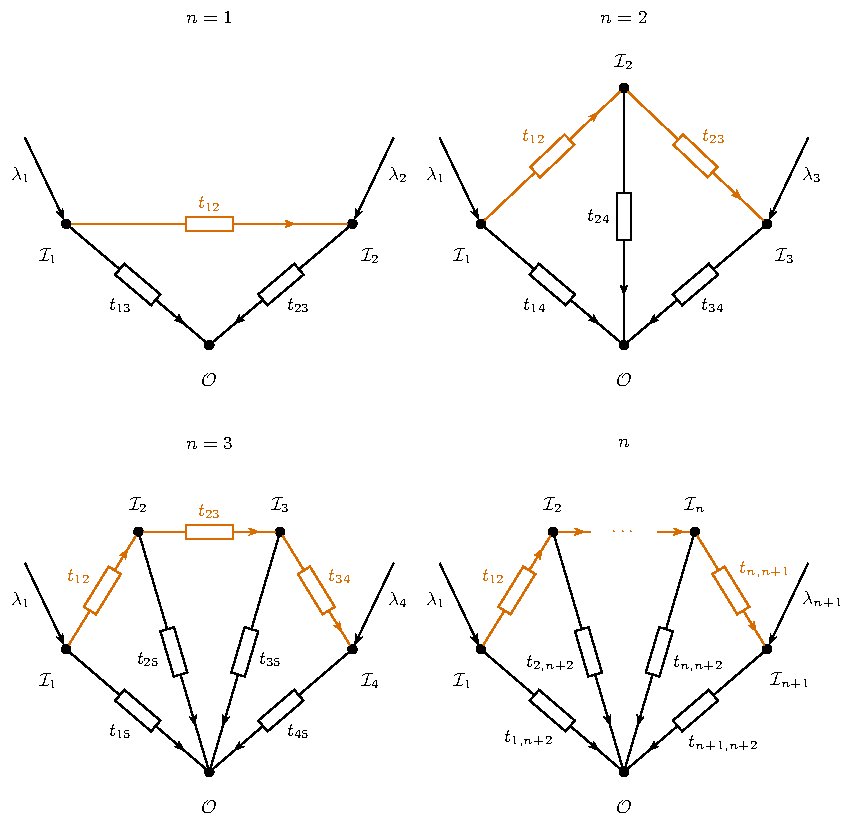
\includegraphics[width=0.96\linewidth,height=.70\textheight,keepaspectratio]{figures/circuits/fa_fan_family.pdf}
\caption{Fans at one, two, three and $n$ loops as circuits, with the interaction path in orange, resistances $t_{vw}$ and injected currents $\lambda_1,\lambda_{n+1}$.}
\label{fig:fan-family}
\end{figure}

By Theorem~\ref{thm:laman-n}, there are $n+1$ interaction vertices besides the insertion $\mathcal O$.

\begin{lemma}[Spokes]\label{lem:spokes}
Let $\deg_\Gamma\mathcal O$ be the number of edges incident to $\mathcal O$ in a graph of Proposition~\ref{prop:cubicfan}. Then $\deg_\Gamma\mathcal O=n+1$: every interaction vertex is joined to $\mathcal O$ by one edge, every interaction vertex is cubic, and exactly two interaction fields remain uncontracted.
\end{lemma}
\begin{proof}[Proof (circuit)]
The uncontracted interaction fields inject the external currents. By Theorems~\ref{thm:no-parallel} and~\ref{thm:laman-n}, with equality in the first step only for cubic vertices,
\begin{equation}\label{eq:cubiccount}
\#(\text{sources})\le3(n+1)-2\bigl(2n+1-\deg_\Gamma\mathcal O\bigr)-\deg_\Gamma\mathcal O
=\deg_\Gamma\mathcal O-n+1\le2 .
\end{equation}
With one source and the drain at $\mathcal O$, every current is a real multiple of the source current and sweeps at most $n<2n$ dimensions; a nonzero kernel therefore has at least two sources, and both inequalities are equalities.
\end{proof}

\begin{lemma}[No interaction cycles]\label{lem:no-cycles}
If every interaction vertex is joined to $\mathcal O$, no set $S$ of interaction vertices carries a cycle.
\end{lemma}
\begin{proof}
A loop of resistors on the interaction nodes $S$, together with their $|S|$ spokes, gives a subcircuit on $S\cup\{\mathcal O\}$ with more resistors than the local count of Ohm's law allows (Theorem~\ref{thm:laman-subgraph}):
\[
|\Gamma_1[S\cup\{\mathcal O\}]|\ge2|S|>2(|S|+1)-3 .
\]
\end{proof}

\begin{proof}[Proof of Proposition~\ref{prop:cubicfan}]
By Lemma~\ref{lem:spokes}, each of the $n+1$ cubic interaction nodes is wired to $\mathcal O$ by one spoke, which leaves $2n+1-(n+1)=n$ internal resistors; they close no loop (Lemma~\ref{lem:no-cycles}) and form a tree. Each node spends one terminal on its spoke and keeps at most two for internal resistors, so the tree is a chain: its interior nodes wire all three terminals, and each end keeps one free terminal, the two sources of Lemma~\ref{lem:spokes}.
\end{proof}

\begin{corollary}[Renormalizable theories]\label{cor:renormalizable}
For every renormalizable $\mathcal N=1$ gauge theory, massless or massive, every nonzero connected graph of $Q_n$, $n\ge1$, with one insertion $\mathcal O$ is a fan of cubic vertices.\footnote{Eliminating a massive multiplet by homotopy transfer, as in Section~\ref{sec:SQEDlift}, generates effective interactions of higher degree among the light fields, in general a formal power series in them; their kernels are those of Section~\ref{sec:forests}.}
\end{corollary}
\begin{proof}
The superpotential has degree at most three, and Proposition~\ref{prop:cubicfan} applies.
\end{proof}

\begin{proposition}[Superpotential vertices and antifield count]\label{prop:cotangent-count}
For the interaction \eqref{eq:B.10}, allow $\bar W(\gamma,\mathsf w)$ to have arbitrary degree. Every nonzero connected $n$-loop graph of $Q_n\mathcal O$ with one insertion $\mathcal O$, $n\ge1$, contains at most one $\bar W$ vertex. Each graph term lowers the number of $\mathsf b,\beta$ factors by $n$ plus the number of $\bar W$ vertices.
\end{proposition}

\begin{lemma}[Antifield terminals]\label{lem:antifield}
Every contraction pairs a $\mathsf b$ or $\beta$ factor with a $\mathsf c$ or $\gamma$ factor. A gauge or matter vertex of \eqref{eq:B.10} supplies one $\mathsf b$ or $\beta$ factor, a $\bar W$ vertex none.
\end{lemma}
\begin{proof}
Each resistor is a contraction of the pairing \eqref{eq:A.20}, which joins a $\mathsf b$ terminal to a $\mathsf c$ terminal or a $\beta$ terminal to a $\gamma$ terminal: every resistor joins an antifield terminal to a field terminal. A gauge or matter node, $\mathsf b\mathsf c\mathsf c$ or $\mathsf c\gamma\beta$ in \eqref{eq:B.10}, has one antifield terminal, a node of $\bar W(\gamma,\mathsf w)$ none.
\end{proof}

\begin{lemma}[Internal edges]\label{lem:internal}
A nonzero connected $n$-loop graph of $Q_n$ has at least $n$ edges between interaction vertices.
\end{lemma}
\begin{proof}
Two resistors from $\mathcal O$ to the same interaction node would be in parallel (Theorem~\ref{thm:no-parallel}), so at most $n+1$ of the $2n+1$ resistors (Theorem~\ref{thm:laman-n}) end at $\mathcal O$, and $2n+1-\deg_\Gamma\mathcal O\ge2n+1-(n+1)=n$ join interaction nodes.
\end{proof}

\begin{proof}[Proof of Proposition~\ref{prop:cotangent-count}]
By Lemmas~\ref{lem:antifield} and~\ref{lem:internal},
\begin{equation}\label{eq:1.15}
\begin{gathered}
\underbrace{n}_{\substack{\deg_\Gamma\mathcal O\le n+1\\
\text{at most }n+1\text{ spokes}}}
\le
\underbrace{2n+1-\deg_\Gamma\mathcal O}_{\text{internal resistors}}
\le
\underbrace{n+1-\#(\bar W\text{ vertices})}_{\substack{
\text{antifield terminals,}\\
\text{one per internal resistor}}}
\\[3pt]
\Longrightarrow\quad\#(\bar W\text{ vertices})\le1,
\end{gathered}
\end{equation}
and each of the $2n+1$ resistors takes one antifield terminal, a $\mathsf b$ or $\beta$ factor:
\begin{equation}\label{eq:antifield-loss}
\begin{aligned}
\#(\mathsf b,\beta\text{ in the output})
&=\#(\mathsf b,\beta\text{ in }\mathcal O)
  +\bigl[n+1-\#(\bar W\text{ vertices})\bigr]-(2n+1)\\
&=\#(\mathsf b,\beta\text{ in }\mathcal O)
  -n-\#(\bar W\text{ vertices}).
\end{aligned}
\end{equation}
\end{proof}

\begin{corollary}[Finite loop order]\label{cor:finite-loop}
For $\bar W$ of any degree, or a formal power series read coefficientwise, $Q_n\mathcal O=0$ for $n>\#(\mathsf b,\beta\text{ in }\mathcal O)$, and terms with a $\bar W$ vertex vanish already for $n+1>\#(\mathsf b,\beta\text{ in }\mathcal O)$.
\end{corollary}
\begin{proof}
The left side of \eqref{eq:antifield-loss} is nonnegative.
\end{proof}
\begin{example}[Field-dependent gauge coupling]\label{ex:field-dependent}
For an abelian gauge factor and a neutral chiral field $\gamma$, a field-dependent gauge kinetic coupling gives
\[
\left.\bar W(\gamma,\mathsf w)\right|_{\mathsf w_{\dot a}=\frac12\partial_{+\dot a}\mathsf c}
=(\partial_{+\dot a}\mathsf c)(\partial_+{}^{\dot a}\mathsf c)
\left(1+\frac{\gamma^2}{m^2}\right)+\cdots,
\]
with $m\ne0$ a mass scale and arbitrarily high powers of $\gamma$ in the omitted terms. Corollary~\ref{cor:finite-loop} bounds the loop order of $Q_n\mathcal O$ by $\#(\mathsf b,\beta\text{ in }\mathcal O)$ for every such degree; compare the bound by operator length in \cite[footnote 8]{BK} and, for pure gauge theory, the letter count of \cite[Equations (3.43)--(3.45)]{semichiral}.
\end{example}

\begin{proposition}[Graphs with one superpotential vertex]\label{prop:superpotential-spider}
For the interaction \eqref{eq:B.10}, a nonzero connected $n$-loop graph of $Q_n$, $n\ge1$, with one insertion $\mathcal O$ and one $\bar W$ vertex joins $\mathcal O$ to all $n+1$ interaction vertices, for any degree of $\bar W$. Removing $\mathcal O$ leaves a tree whose arms meet at $\bar W$.
\end{proposition}
\begin{proof}
With one $\bar W$ vertex the two bounds in \eqref{eq:1.15} coincide:
\begin{equation}\label{eq:superpotential-spokes}
n\le2n+1-\deg_\Gamma\mathcal O\le n
\quad\Longrightarrow\quad
\deg_\Gamma\mathcal O=n+1,
\end{equation}
so every interaction node is wired to $\mathcal O$, and the $n$ internal resistors close no loop (Lemma~\ref{lem:no-cycles}) and form a tree. A cubic node keeps at most two internal resistors besides its spoke, so the tree branches only at the $\bar W$ node; with $a$ arms of $\ell_i$ cubic nodes,
\begin{equation}\label{eq:1.16}
\begin{gathered}
\Gamma\setminus\{\mathcal O\}
=\text{arms of lengths }\ell_1,\ldots,\ell_a\text{ meeting at }\bar W,\\
\ell_1+\cdots+\ell_a=n,\qquad\ell_i\ge1,\qquad\deg\bar W\ge a+1,
\end{gathered}
\end{equation}
where $\deg\bar W$, the number of field factors of the contributing monomial, covers the $a$ internal resistors at the $\bar W$ node and its spoke.
\end{proof}
\begin{remark}
With at most two arms the graph of Proposition~\ref{prop:superpotential-spider} is a fan; the bound $a+1\le\deg\bar W$ gives this case for $\deg\bar W\le3$.
\end{remark}

\begin{corollary}[Graphs of $Q_n$]\label{cor:graphs-Qn}
For the interaction \eqref{eq:B.10}, every nonzero connected graph of $Q_n$, $n\ge1$, with one insertion $\mathcal O$ is a fan, or a spider whose arms meet at its $\bar W$ vertex, a book when all its arms have length one (Definition~\ref{def:spiders-books}); for $\deg\bar W\le3$ it is a fan.
\end{corollary}
\begin{proof}
Propositions~\ref{prop:cubicfan}, \ref{prop:cotangent-count} and~\ref{prop:superpotential-spider}.
\end{proof}

\begin{proposition}[Superpotential vertices with two insertions]\label{prop:product-superpotential}
Let $\Gamma$ be a nonzero connected marked graph of the quantum product \eqref{eq:star} at order $\hbar^n$, $n\ge1$, with insertions $A,B$, for the interaction \eqref{eq:B.10} with $\bar W$ of any degree.
\begin{enumerate}
\item[(i)] Every connected component of $\Gamma\setminus\{A,B\}$ contains at most one $\bar W$ vertex.
\item[(ii)] Each graph term satisfies
\begin{equation}\label{eq:product-antifield-loss}
\#(\mathsf b,\beta\text{ in the output})
=\#(\mathsf b,\beta\text{ in }A)+\#(\mathsf b,\beta\text{ in }B)-n-\#(\bar W\text{ vertices}),
\end{equation}
so the order-$\hbar^n$ term vanishes unless $\#(\mathsf b,\beta\text{ in }A)+\#(\mathsf b,\beta\text{ in }B)\ge n+\#(\bar W\text{ vertices})$.
\end{enumerate}
\end{proposition}
\begin{proof}
(i) The $|T_j|$ nodes of a component $T_j$ are connected through its internal resistors $I_j$, each of which takes its antifield terminal from a node of $T_j$ (Lemma~\ref{lem:antifield}):
\[
|T_j|-1\le|I_j|\le|T_j|-\#(\bar W\text{ vertices in }T_j).
\]
(ii) Each of the $2n$ physical resistors takes one antifield terminal, the $n$ interaction nodes have $n-\#(\bar W\text{ vertices})$ of them, and the marked resistor contracts the auxiliary pair $a,b_{\mathrm{aux}}$ of \eqref{eq:1.3}.
\end{proof}
The graphs of the quantum product are forests of interaction trees attached to both insertions, classified in Proposition~\ref{prop:product-forest}.

\section{Fan kernels}
\label{sec:fans}

In four dimensions, a renormalizable $\mathcal N=1$ supersymmetric gauge theory has a superpotential of degree at most three, and its holomorphic gauge and matter vertices are cubic. The Laman constraints therefore force every nonzero connected graph contributing to a loop correction of the supercharge to be a fan (Figure~\ref{fig:fan-family}). The fan kernels therefore determine every loop correction to the supersymmetry transformation in these theories, and our aim in this section is to evaluate them at every loop order. In the original Schwinger times their integrands are rational, with powers of the spanning-tree polynomial in the denominator \cite[Corollaries 1--2]{Wang},\footnote{Fans are Laman graphs of type~I$'$. For such graphs Gui, Wang and Williams wrote the weights recursively from the $L_\infty$ relations as integrals over unit cubes with polynomial integrands at each order in the displacements \cite[Theorem 4.13]{GWW}, so that within this formalism every Taylor coefficient is computable in principle, and they evaluated the fans through three loops \cite[Sections 4.4--4.6]{GWW}; the relation of their cube parameters to Schwinger parameters is left open in \cite[Remark 4.14]{GWW}.} so the cost of evaluating them grows exponentially with the loop order, and they lack a physical picture. We derive positive coordinates, the parallel current-division ratios of the circuit, from the Schwinger integral itself by series and parallel reductions of the associated circuit diagrams, applied by induction on the loop order. In our coordinates the currents are polynomial and every Taylor coefficient is a finite factorial sum, and we evaluate the kernels in closed form for every $n$. Appendix~\ref{sec:network} gives the detailed reductions.

\subsection{The one-loop triangle diagram}

The one-loop triangle kernel is known \cite[Equations (4.15)--(4.20)]{operatope}, \cite[Equations (2.45)--(2.48)]{BK}, \cite[Equations (4.1)--(4.5)]{GWW}; we rederive it for the triangle in Figure~\ref{fig:low-fans} to fix the orientation and normalization used below and to introduce the physical picture of the circuit.
\begin{figure}[H]
\centering
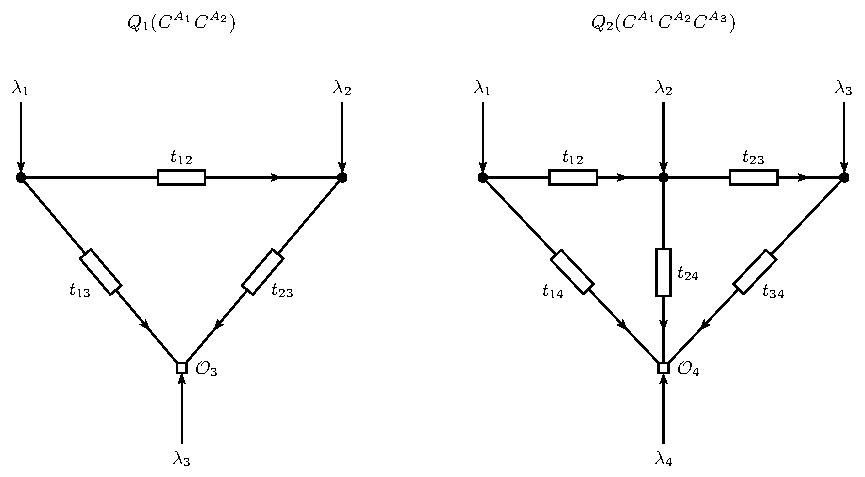
\includegraphics[width=0.94\linewidth,height=.70\textheight,keepaspectratio]{figures/circuits/fans_low.pdf}
\caption{The one- and two-loop fan circuits. Dots are interaction vertices and the square is the local insertion. Each edge carries a resistor $t_{vw}$; $\lambda_v$ is the current injected at vertex $v$.}
\label{fig:low-fans}
\end{figure}
\noindent Its vertices are $1,2,3$, with $3$ at the origin. With $t_{12}+t_{13}+t_{23}=1$, current conservation and the cycle equation give\footnote{The first line of \eqref{eq:triangle-current} is read off from $\partial y_{12}/\partial\lambda_1=t_{13}$ and $\partial y_{12}/\partial\lambda_2=-t_{23}$. With $\lambda_2$ switched off, the current $\lambda_1$ enters at vertex $1$ and leaves at vertex $3$ through the two parallel paths $1\to3$ and $1\to2\to3$; the path through edge $12$, of resistance $t_{12}+t_{23}$, carries the fraction $t_{13}/(t_{12}+t_{13}+t_{23})=t_{13}$. With $\lambda_1$ switched off, the current $\lambda_2$ enters at $2$, and the path $2\to1\to3$ carries the fraction $t_{23}$ against the orientation of edge $12$. The other two lines are current conservation at vertices $1$ and $2$.}
\begin{equation}\label{eq:triangle-current}
\begin{aligned}
y_{12,+\dot a}&=t_{13}\lambda_{1,+\dot a}-t_{23}\lambda_{2,+\dot a},\\
y_{13,+\dot a}&=\lambda_{1,+\dot a}-y_{12,+\dot a},\\
y_{23,+\dot a}&=\lambda_{2,+\dot a}+y_{12,+\dot a}.
\end{aligned}
\end{equation}
Use simplex coordinates $r_1,r_2$ with $(t_{12},t_{13},t_{23})=(1-r_1-r_2,r_1,r_2)$. The Jacobian is
\begin{equation}
-dy_{12,+\dot+}\wedge dy_{12,+\dot-}
=(\lambda_{1,+\dot a}\lambda_{2,+}{}^{\dot a})\,dr_1\wedge dr_2.
\end{equation}
Consequently,

\begin{equation}\label{eq:1.25}
\begin{aligned}
\mathcal I_\triangle^{\mathrm{raw\ cut}}(\lambda;z)
&=(\lambda_{1,+\dot a}\lambda_{2,+}{}^{\dot a})
\int_0^1dr_1\int_0^{1-r_1}dr_2\,
e^{-\sum_e y_{e,+\dot b}z_e^{+\dot b}},\\
\mathcal I_\triangle^{\mathrm{raw\ cut}}(\lambda;0)
&=\frac12\lambda_{1,+\dot a}\lambda_{2,+}{}^{\dot a}.
\end{aligned}
\end{equation}

Expanding the exponential and integrating each monomial yields the entire displacement dependence, as in \cite[Equation (2.47)]{BK}:\footnote{Apart from the prefactor, the displacements enter through one independent combination, the loop sum $z_{12}+z_{23}+z_{31}$ with $z_{31}=-z_{13}$, which multiplies the loop current $y_{12}$ in the exponent. As in \eqref{eq:input-displacement}, the displacements generate the holomorphic derivatives of the letters of $\mathcal O$.}

\begin{equation}\label{eq:1.46}
\begin{aligned}
\mathcal I_\Gamma^{\mathrm{raw\ cut}}(\lambda;z)
={}&(\lambda_{1,+\dot a}\lambda_{2,+}{}^{\dot a})\,
 e^{-\lambda_{1,+\dot a}z_{13}^{+\dot a}-\lambda_{2,+\dot a}z_{23}^{+\dot a}}\\
&\times\sum_{i,j\ge0}
\frac{[-\lambda_{1,+\dot b}(z_{12}+z_{23}-z_{13})^{+\dot b}]^i
[\lambda_{2,+\dot c}(z_{12}+z_{23}-z_{13})^{+\dot c}]^j}{(i+j+2)!}.
\end{aligned}
\end{equation}

\subsection{One elimination step}
\label{sec:fan-step}

The fan is reduced recursively: each step eliminates the leftmost vertex and redistributes its source between the two remaining endpoints. For the $n$-loop fan of Figure~\ref{fig:fan-family}, with path $1\to2\to\cdots\to n+1$, spokes oriented towards the insertion $n+2$, and $n\ge2$, the first step is the following (Figure~\ref{fig:B-fan-first-elimination}).

\begin{proposition}[One elimination step]\label{prop:fan-step}
Set
\[
r_1=\frac{t_{1,n+2}}{t_{12}+t_{1,n+2}},\qquad
r_2=\frac{t_{12}+t_{1,n+2}}{t_{12}+t_{1,n+2}+t_{2,n+2}},
\]
the fraction of $\lambda_1$ passed to vertex $2$ and the fraction of the merged spoke current carried by the original spoke $(2,n+2)$. Eliminating vertex $1$ replaces the resistors $t_{12},t_{1,n+2},t_{2,n+2}$ by one resistor between $2$ and $n+2$ and moves the source $\lambda_1$ to the remaining endpoints:
\[
t^{\mathrm{red}}_{2,n+2}=\left[\frac1{t_{12}+t_{1,n+2}}+\frac1{t_{2,n+2}}\right]^{-1},\qquad
\lambda^{\mathrm{red}}_2=\lambda_2+r_1\lambda_1,\qquad
\lambda^{\mathrm{red}}_{n+2}=\lambda_{n+2}+(1-r_1)\lambda_1 .
\]
The removed currents follow from the reduced spoke current $y^{\mathrm{red}}_{2,n+2}=\lambda_2+r_1\lambda_1-y_{23}$:
\[
y_{2,n+2}=r_2y^{\mathrm{red}}_{2,n+2},\qquad
y_{12}=r_1r_2\lambda_1-(1-r_2)\lambda_2+(1-r_2)y_{23},\qquad
y_{1,n+2}=\lambda_1-y_{12}.
\]
\end{proposition}
\begin{proof}
Conservation at $1$ and the cycle $1\to2\to n+2\to1$ give \eqref{eq:B-fan-first-cycle}:
\[
y_{1,n+2}=\lambda_1-y_{12},\qquad
t_{2,n+2}y_{2,n+2}=t_{1,n+2}\lambda_1-(t_{12}+t_{1,n+2})y_{12}.
\]
The resistors on $2\to1\to n+2$ combine in series, of resistance $t_{12}+t_{1,n+2}$, and carry
\[
r_1\lambda_1-y_{12}=\frac{t_{2,n+2}y_{2,n+2}}{t_{12}+t_{1,n+2}} .
\]
In parallel with $t_{2,n+2}$ the conductances add, and the merged current $y^{\mathrm{red}}_{2,n+2}=(r_1\lambda_1-y_{12})+y_{2,n+2}$ divides as
\[
r_1\lambda_1-y_{12}=(1-r_2)\,y^{\mathrm{red}}_{2,n+2},\qquad
y_{2,n+2}=r_2\,y^{\mathrm{red}}_{2,n+2},
\]
while conservation at $2$ in the reduced network gives $y^{\mathrm{red}}_{2,n+2}=\lambda^{\mathrm{red}}_2-y_{23}$. Solving for $y_{12}$ gives the stated formula.
\end{proof}
\begin{figure}[H]
\centering
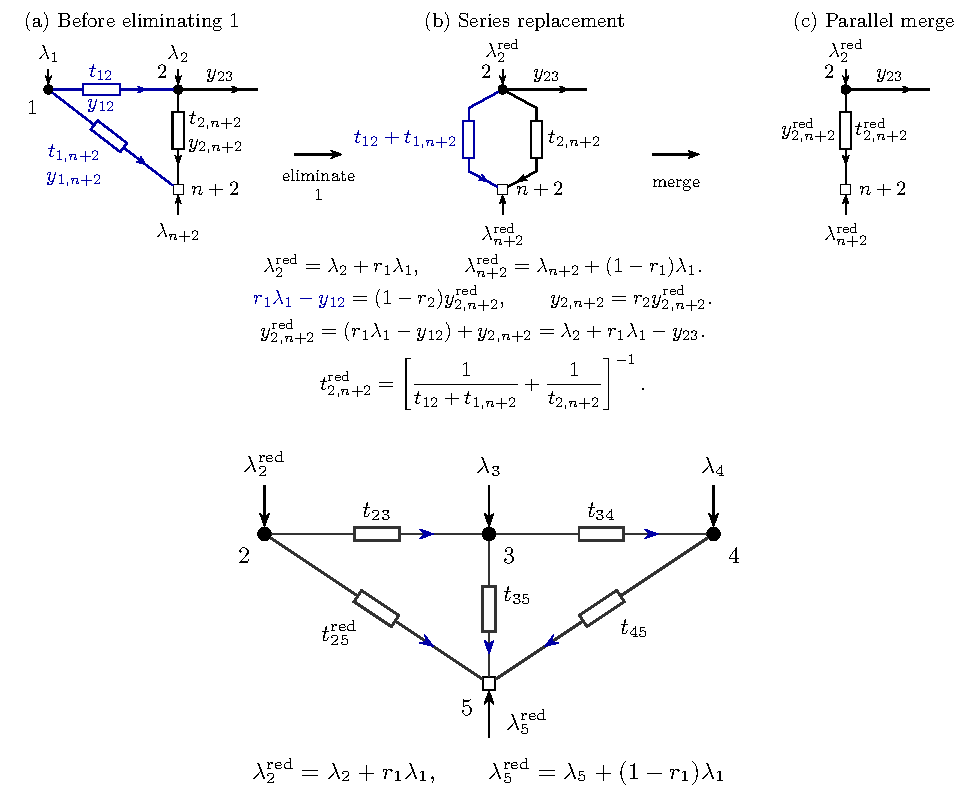
\includegraphics[width=\linewidth]{figures/circuits/fan_one_step.pdf}
\caption{One elimination step on the $n$-loop fan (Proposition~\ref{prop:fan-step}). (a) The resistors $t_{12},t_{1,n+2}$ (blue) at vertex $1$; (b) their series replacement, with $\lambda_1$ redistributed to vertex $2$ and to the insertion; (c) the parallel merge with the spoke $t_{2,n+2}$. Below: the three-loop network after eliminating vertex $1$, on which the next step acts at vertex $2$.}
\label{fig:B-fan-first-elimination}
\end{figure}
The next step acts on vertex $2$ with the reduced source $\lambda_2+r_1\lambda_1$ and the reduced spoke $t^{\mathrm{red}}_{2,n+2}$ (Appendix~\ref{sec:B-fan-reduction}). For the kernel, the step is an integral of the $(n-1)$-loop fan kernel over $r_1,r_2$, \eqref{eq:fan-kernel-recursion} of Theorem~\ref{thm:kernel-series-parallel}.

\subsection{Positive coordinates at arbitrary order}
\label{sec:fan-positive}

The $n$-loop fan in Figure~\ref{fig:general-fan} has an interaction path $1-2-\cdots-(n+1)$ and a spoke from each path vertex to the insertion $n+2$. Order its edges as

\begin{equation}\label{eq:1.32}
\begin{gathered}
\Gamma_1=((1,2),(1,n+2),\ldots,(n,n+1),(n,n+2),(n+1,n+2)),\\
n=1:\qquad(t_{12},t_{13},t_{23})=(1-r_1-r_2,r_1,r_2).
\end{gathered}
\end{equation}
\begin{figure}[H]
\centering
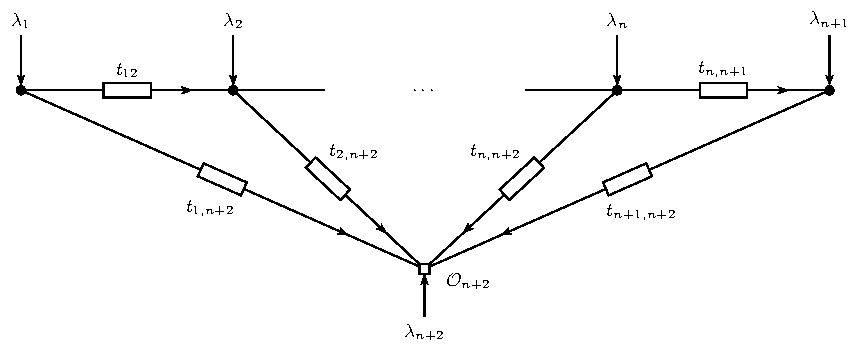
\includegraphics[width=0.94\linewidth,height=.70\textheight,keepaspectratio]{figures/circuits/fan_general.pdf}
\caption{The $n$-loop fan circuit: a path of $n+1$ cubic interactions joined to the insertion. The resistors have resistances $t_{vw}$, and the external arrows carry the currents $\lambda_v$. The short stubs and central ellipsis indicate omitted intermediate vertices.}
\label{fig:general-fan}
\end{figure}


We keep the sources $\lambda_2,\ldots,\lambda_n$. In a renormalizable theory they vanish: the vertices $1$ and $n+1$ alone carry output letters, and hence injected currents. The iteration admits currents at $2,\ldots,n$, and in a nonrenormalizable theory one of these vertices can be a superpotential vertex of higher degree; by Propositions~\ref{prop:cotangent-count} and~\ref{prop:superpotential-spider}, at most one of $\lambda_2,\ldots,\lambda_n$ is nonzero in every fan kernel considered here.

For $n\ge2$, iterating Proposition~\ref{prop:fan-step} along the interaction path, at vertex $1$, then vertex $2$, and so on, reduces the fan to the triangle. Reversing the eliminations derived in Appendix~\ref{sec:B-fan-reduction} gives the positive edge Schwinger times in terms of the dimensionless reduction coordinates $r_1,\ldots,r_{2n}$:\footnote{Equation~\eqref{eq:1.36} solves the recursion \eqref{eq:B-fan-inverse-times},
\[
t^{\mathrm{red}}_{i,n+2}=\frac{r_{2i-1}}{1-r_{2i}}\,t^{\mathrm{red}}_{i+1,n+2},\qquad
t_{i,i+1}=\frac{1-r_{2i-1}}{1-r_{2i}}\,t^{\mathrm{red}}_{i+1,n+2},\qquad
t_{i+1,n+2}=\frac{t^{\mathrm{red}}_{i+1,n+2}}{r_{2i}},
\]
backwards from the final triangle $(t^{\mathrm{red}}_{n,n+2},t_{n,n+1},t_{n+1,n+2})=(r_{2n-1},1-r_{2n-1}-r_{2n},r_{2n})$ down to $t_{1,n+2}=t^{\mathrm{red}}_{1,n+2}$; each step inverts the series sum and the parallel merge of Proposition~\ref{prop:fan-step}.}

\begin{equation}\label{eq:1.36}
\begin{aligned}
t_{i,i+1}&=\frac{(1-r_{2i-1})\prod_{j=i+1}^{n}r_{2j-1}}{\prod_{j=i}^{n-1}(1-r_{2j})},&&1\leq i<n,\\
t_{1,n+2}&=\frac{\prod_{j=1}^{n}r_{2j-1}}{\prod_{j=1}^{n-1}(1-r_{2j})},&&
t_{i,n+2}=\frac{\prod_{j=i}^{n}r_{2j-1}}{r_{2i-2}\prod_{j=i}^{n-1}(1-r_{2j})},\quad 2\leq i\leq n,\\
t_{n,n+1}&=1-r_{2n-1}-r_{2n},&&t_{n+1,n+2}=r_{2n},
\end{aligned}
\end{equation}
Figure~\ref{fig:fan-reduction} shows the first reduction at two loops.
\begin{figure}[H]
\centering
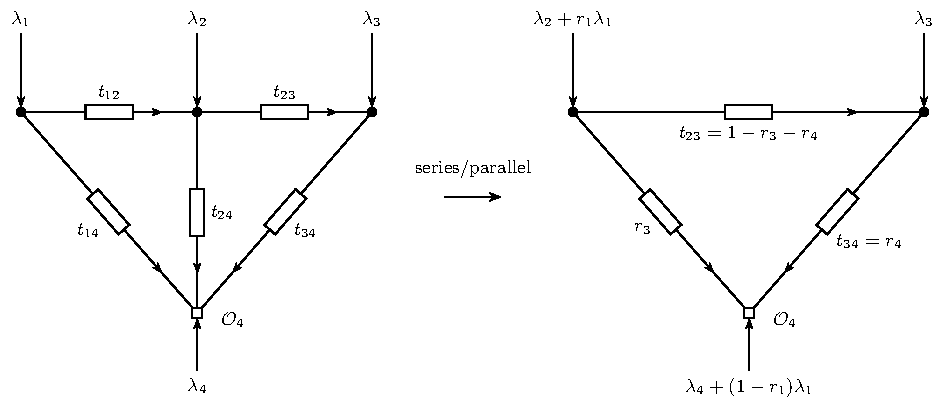
\includegraphics[width=0.94\linewidth,height=.70\textheight,keepaspectratio]{figures/circuits/positive_chart.pdf}
\caption{Two-loop circuit reduction. Eliminating vertex $1$ combines its resistances in series and parallel and redistributes $\lambda_1$ between its neighbours. The $r_j$ are the reduction coordinates of \eqref{eq:1.36}.}
\label{fig:fan-reduction}
\end{figure}

\noindent The independent coordinates range over

\begin{equation}\label{eq:1.37}
0<r_j<1\quad(1\leq j\leq2n-2),\qquad r_{2n-1}>0,\quad r_{2n}>0,\quad r_{2n-1}+r_{2n}<1 .
\end{equation}

The final two coordinates form a triangle; the earlier coordinates range independently over intervals. {\boldmath\bfseries Each $r_j$ with $j\le2n-2$ is a current-division ratio of the iteration: $r_{2i-1}$ is the fraction of the source at the eliminated vertex $i$ that the series step passes to vertex $i+1$, and $r_{2i}$ is the fraction of the merged current carried by the original spoke $(i+1,n+2)$ after the parallel merge.} The last two, $r_{2n-1}$ and $r_{2n}$, are the simplex coordinates of the final triangle, as in \eqref{eq:1.25}. Reversing the reductions solves all conservation and cycle equations. Along the path,\footnote{Equation~\eqref{eq:1.38} is Proposition~\ref{prop:fan-step} applied at vertex $i$ of the reduced network,
\[
y_{i,i+1}=r_{2i-1}r_{2i}\lambda^{\mathrm{red}}_i-(1-r_{2i})\lambda_{i+1}+(1-r_{2i})y_{i+1,i+2},\qquad
\lambda^{\mathrm{red}}_i=\lambda_i+r_{2i-3}\lambda^{\mathrm{red}}_{i-1},\quad\lambda^{\mathrm{red}}_1=\lambda_1,
\]
with the resistance ratios $r_{2i-1}=t^{\mathrm{red}}_{i,n+2}/(t_{i,i+1}+t^{\mathrm{red}}_{i,n+2})$ and $r_{2i}=(t_{i,i+1}+t^{\mathrm{red}}_{i,n+2})/(t_{i,i+1}+t^{\mathrm{red}}_{i,n+2}+t_{i+1,n+2})$ of \eqref{eq:B-fan-general-fractions}; the last line is the triangle \eqref{eq:triangle-current} with $t_{13},t_{23}$ replaced by $t^{\mathrm{red}}_{n,n+2}=r_{2n-1}$ and $t_{n+1,n+2}=r_{2n}$.}

\begin{equation}\label{eq:1.38}
\begin{aligned}
y_{n,n+1,+\dot a}
&=r_{2n-1}\sum_{j=1}^{n}
\left(\prod_{k=j}^{n-1}r_{2k-1}\right)\lambda_{j,+\dot a}
-r_{2n}\lambda_{n+1,+\dot a},\\
y_{i,i+1,+\dot a}
&=r_{2i-1}r_{2i}\sum_{j=1}^{i}
\left(\prod_{k=j}^{i-1}r_{2k-1}\right)\lambda_{j,+\dot a}\\
&\quad-(1-r_{2i})\lambda_{i+1,+\dot a}
+(1-r_{2i})y_{i+1,i+2,+\dot a},\qquad1\le i<n.
\end{aligned}
\end{equation}
and the spoke currents are

\begin{equation}\label{eq:1.39}
\begin{aligned}
y_{1,n+2,+\dot a}&=\lambda_{1,+\dot a}-y_{12,+\dot a},\\
y_{i,n+2,+\dot a}&=\lambda_{i,+\dot a}+y_{i-1,i,+\dot a}-y_{i,i+1,+\dot a},
\qquad2\le i\le n,\\
y_{n+1,n+2,+\dot a}&=\lambda_{n+1,+\dot a}+y_{n,n+1,+\dot a}.
\end{aligned}
\end{equation}
This reflects the order of our iteration: the path currents are fixed first, backwards from $y_{n,n+1}$ to $y_{12}$, and current conservation at each path vertex then determines every spoke current.

The recursion \eqref{eq:1.38} is lower triangular. The Jacobian is therefore block lower triangular, and its determinant is the product of the $2\times2$ diagonal blocks; see Appendix~\ref{sec:B-fan-reduction} for details. Hence

\begin{equation}\label{eq:1.40}
\begin{aligned}
\mathcal I_\Gamma^{\mathrm{raw\ cut}}(\lambda;z)
={}&\int_{\eqref{eq:1.37}}d^{2n}r\,
\prod_{i=1}^{n-1}\underbrace{r_{2i}
\left[\sum_{j=1}^{i}\left(\prod_{k=j}^{i-1}r_{2k-1}\right)
\lambda_{j,+\dot a_i}\right]
(\lambda_{i+1,+}{}^{\dot a_i}-y_{i+1,i+2,+}{}^{\dot a_i})}_{\text{Jacobian block of step }i:\ \partial y_{i,i+1}/\partial(r_{2i-1},r_{2i})}\\
&\times\underbrace{\left[\sum_{j=1}^{n}
\left(\prod_{k=j}^{n-1}r_{2k-1}\right)\lambda_{j,+\dot b}\right]
\lambda_{n+1,+}{}^{\dot b}}_{\text{Jacobian block of the final triangle:}\ \partial y_{n,n+1}/\partial(r_{2n-1},r_{2n})}
\,e^{-\sum_e y_{e,+\dot a}z_e^{+\dot a}}.
\end{aligned}
\end{equation}

Here $y_{i+1,i+2}$ is the path current of the following step, expressed in the $r$ coordinates by the recursion \eqref{eq:1.38}; the bracket in each block is the source at vertex $i$ after the earlier eliminations. All currents are polynomial in the new coordinates, with no spanning-tree denominator, so every fixed Taylor coefficient is a polynomial integral over the explicit domain \eqref{eq:1.37}, for arbitrary sources on the path. For $n=1$, the products over $i<n$ are empty and \eqref{eq:1.40} reduces to the triangle.

\subsection{Endpoint sources and Taylor expansion}

Section~\ref{sec:fan-positive} evaluated the fan kernel for arbitrary sources and displacements. In the computation of $Q_n$ in a renormalizable theory, each interior interaction vertex has two path edges and one spoke, so all three factors of its cubic monomial are contracted and the two endpoints alone retain an output field; hence $\lambda_2=\cdots=\lambda_n=0$. The interaction vertices carry no derivatives, so only the holomorphic derivatives of the letters of $\mathcal O$ generate displacements. These sit on the spokes: $z_{i,i+1}=0$ and $z_{i,n+2}=-z_i$, where $z_i$ displaces the letter contracted on spoke $i$. The density then factorizes:

\begin{equation}\label{eq:1.41}
\begin{aligned}
&\mathcal I_\Gamma^{\mathrm{raw\ cut}}(\lambda;z)
\big|_{\lambda_2=\cdots=\lambda_n=0,
\ z_{i,i+1}=0,\ z_{i,n+2}=-z_i}\\
&=(\lambda_{1,+\dot a}\lambda_{n+1,+}{}^{\dot a})^n
\int_{\eqref{eq:1.37}}d^{2n}r\,
\left[\prod_{j=1}^{n-1}r_{2j-1}^{n-j}r_{2j}(1-r_{2j})^{j-1}\right]
r_{2n}^{n-1}
e^{\sum_j y_{j,n+2,+\dot a}z_j^{+\dot a}}.
\end{aligned}
\end{equation}

The exponential in \eqref{eq:1.41} translates the two endpoint fields. Substituting the currents \eqref{eq:1.38}--\eqref{eq:1.39} gives
\begin{equation}\label{eq:fan-output-translation}
\sum_{j=1}^{n+1}y_{j,n+2,+\dot a}(r)z_j^{+\dot a}
=\lambda_{1,+\dot a}x_1^{+\dot a}(r,z)
+\lambda_{n+1,+\dot a}x_{n+1}^{+\dot a}(r,z),
\end{equation}
where the translated positions are
\begin{equation}\label{eq:fan-output-points}
\begin{aligned}
x_1^{+\dot a}(r,z)
={}&\sum_{j=1}^{n}(1-r_{2j-1})
\left(\prod_{k=1}^{j-1}r_{2k-1}\right)\\
&\times\left[
\left(\prod_{k=1}^{j-1}(1-r_{2k})\right)z_1^{+\dot a}
+\sum_{i=2}^{j}r_{2i-2}
\left(\prod_{k=i}^{j-1}(1-r_{2k})\right)z_i^{+\dot a}
\right]\\
&+\left(\prod_{k=1}^{n}r_{2k-1}\right)z_{n+1}^{+\dot a},\\[3pt]
x_{n+1}^{+\dot a}(r,z)
={}&r_{2n}\left[
\left(\prod_{k=1}^{n-1}(1-r_{2k})\right)z_1^{+\dot a}
+\sum_{i=2}^{n}r_{2i-2}
\left(\prod_{k=i}^{n-1}(1-r_{2k})\right)z_i^{+\dot a}
\right]\\
&+(1-r_{2n})z_{n+1}^{+\dot a}.
\end{aligned}
\end{equation}

We now give the Taylor expansion in explicit form, ready for direct use in the machine enumeration of the later sections. The monomial moments on the parameter domain are

\begin{equation}\label{eq:1.44}
\int_{\eqref{eq:1.37}}dr_1\cdots dr_{2n}\,\prod_{j=1}^{2n}r_j^{m_j}=\frac{m_{2n-1}!\,m_{2n}!}{(m_{2n-1}+m_{2n}+2)!}\prod_{j=1}^{2n-2}\frac1{m_j+1},
\end{equation}

For arbitrary edge displacements, sum over nonnegative integers $r_0,s_0,r_{ik},s_i$, with $1\le i\le k\le n$. Grouping by the total displacement degree $m$, the full Taylor expansion is
\begin{equation}\label{eq:fan-full-taylor}
\begin{aligned}
&\left.\mathcal I_\Gamma^{\mathrm{raw\ cut}}(\lambda;z)
\right|_{\lambda_2=\cdots=\lambda_n=0}\\
&=(\lambda_{1,+\dot a}\lambda_{n+1,+}{}^{\dot a})^n
\sum_{m=0}^{\infty}
\sum_{\substack{r_0,s_0,r_{ik},s_i\ge0\\
r_0+s_0+\sum_{i=1}^ns_i+\sum_{k=1}^n\sum_{i=1}^kr_{ik}=m}}\\
&\quad\times
\frac{[-\lambda_{1,+\dot b}z_{1,n+2}^{+\dot b}]^{r_0}
[-\lambda_{n+1,+\dot c}z_{n+1,n+2}^{+\dot c}]^{s_0}}
{r_0!s_0!}\\
&\quad\times\prod_{1\le i\le k\le n}
\frac{\left[-\lambda_{1,+\dot d}
(z_{i,i+1}+z_{i+1,n+2}-z_{i,n+2})^{+\dot d}\right]^{r_{ik}}}
{r_{ik}!}\\
&\quad\times\prod_{i=1}^n
\frac{\left[\lambda_{n+1,+\dot e}
(z_{i,i+1}+z_{i+1,n+2}-z_{i,n+2})^{+\dot e}\right]^{s_i}}
{s_i!}\\
&\quad\times
\frac{\left(\sum_{i=1}^nr_{in}\right)!
\left(n-1+\sum_{i=1}^ns_i\right)!}
{\left(n+1+\sum_{i=1}^nr_{in}+\sum_{i=1}^ns_i\right)!}\\
&\quad\times\prod_{j=1}^{n-1}
\frac{1}{n-j+1+\sum_{k=j}^{n}\sum_{i=1}^{k}r_{ik}}\\
&\quad\times\prod_{j=1}^{n-1}
\frac{
\left(1+\sum_{i=1}^{j}r_{ij}\right)!
\left(j-1+\sum_{i=1}^{j}\left[s_i+\sum_{k=j+1}^{n}r_{ik}\right]\right)!}
{\left(j+1+\sum_{i=1}^{j}\left[s_i+\sum_{k=j}^{n}r_{ik}\right]\right)!}.
\end{aligned}
\end{equation}
Its simplest coefficient, without displacements, is
\begin{equation}\label{eq:1.42}
\left.\mathcal I_\Gamma^{\mathrm{raw\ cut}}(\lambda;0)\right|_{\lambda_{2,+\dot a}=\cdots=\lambda_{n,+\dot a}=0}
=\frac{(\lambda_{1,+\dot a}\lambda_{n+1,+}{}^{\dot a})^n}{(n!)^3(n+1)}.
\end{equation}
For $n=1,2,3$, \eqref{eq:1.42} reproduces \cite[Equations (4.20), (4.44), (4.67)]{operatope}, \cite[Equation (2.48)]{BK} and \cite[Sections 4.4--4.6]{GWW}.

\clearpage
\section{More general superpotentials and product forests}
\label{sec:forests}

Two computations lead beyond the fans:
\begin{enumerate}
\item the quantum product compatible with the loop-corrected supercharge joins two insertions, and its graphs are forests of interaction trees attached to both, the marked books among them;
\item for a superpotential of degree greater than three, the loop corrections to the supersymmetry transformation themselves contain spiders and books (Proposition~\ref{prop:superpotential-spider}).
\end{enumerate}

We first review the quantum product defined by Gaiotto, Kulp and Wu~\cite{higher}. Physically, it is the normal-ordered product of an interacting conformal or holomorphic theory, defined by the contour integral \eqref{eq:ring-normal-ordering} of one operator around the other (Theorem~\ref{thm:normal-ordering}). For the enumeration of $\mathbf Q$-cohomology representatives, it repairs the Leibniz rule, which the loop corrections $Q_n$ violate for the ordinary product: $\mathbf Q$ is a graded derivation of the quantum product (Section~\ref{sec:dressed-chain}), so the product of two $\mathbf Q$-closed operators is closed and, up to $\mathbf Q$-exact terms, depends only on their classes. The BPS cohomology thereby recovers its ring structure (Theorem~\ref{thm:quantum-bps-ring}): a product of quantum cocycles is again a quantum cocycle, and it is lifted exactly when it becomes a quantum coboundary, which greatly reduces the lifting tests needed in practice (Section~\ref{sec:lifting}).

\subsection{The quantum product}
\label{sec:dressed-definition}

Starting at one loop, $\mathbf Q$ does not obey the Leibniz rule for the ordinary product of local operators. In $\mathcal N=4$ Yang--Mills theory the one-loop operator, the case $n=1$ of Theorem~\ref{thm:N4-allloop}, is the simplex integral
\begin{equation}\label{eq:2.16}
\begin{aligned}
Q_1={}&-\frac{1}{64\pi^2}
\int_0^1dr_2\int_0^{1-r_2}dr_1\int d^3\theta\int d^4z_1\,d^4z_2\,
C_{ARD}C_{BRE}\\
&\times(\partial_{+\dot a}C^D)
\big(x+(1-r_1)z_1+r_1z_2,\theta\big)\,
(\partial_+{}^{\dot a}C^E)
\big(x+r_2z_1+(1-r_2)z_2,\theta\big)\\
&\times\frac{\delta}{\delta C^A(x+z_1,\theta)}
\frac{\delta}{\delta C^B(x+z_2,\theta)}.
\end{aligned}
\end{equation}
with the superfield $C$ of Appendix~\ref{sec:N4-superfield} and the functional derivatives normalized by \eqref{eq:2.10}. Its two functional derivatives contract two input letters, which can belong to different factors (equation~\eqref{eq:2.29} of Section~\ref{sec:product}). The quantum product corrects the ordinary product by marked graphs. Let $A,B$ be homogeneous holomorphic local operators, with $|A|$ the fermion number of $A$. Their quantum product is the interacting marked operation of \cite[Equations (4.18) and (4.45)]{higher} with a single marked edge, that is, the loop-corrected regularized product of \cite[Section 4.3 and Figure 7]{higher}. Introduce a decoupled free pair $a,b_{\mathrm{aux}}$, of fermion numbers $0,1$, with action $\int\Omega\wedge[a\bar\partial b_{\mathrm{aux}}]_{(0,2)}$. Contracting this pair between $Aa$ and $b_{\mathrm{aux}}B$ marks the edge $AB$:

\begin{equation}\label{eq:1.3}
{\gamma=\{(A,B)\}},\qquad
\{\mathcal I^{\otimes n},A,B\}^{\gamma,0}
=\left.\{\mathcal I^{\otimes n},Aa,b_{\mathrm{aux}}B\}_0\right|_{\mathrm{aux}=0}.
\end{equation}

The restriction $\mathrm{aux}=0$ sets the auxiliary fields to zero after contraction. The edge $AB$ is last in Wick order, has $z_{AB}=0$, and its positive Schwinger time is integrated along with those of the physical edges. At order zero, the left derivatives give

\begin{equation}\label{eq:1.4}
\{A,B\}^{\gamma,0}
=(-1)^{|A|}\frac{\partial_L}{\partial a}\frac{\partial_L}{\partial b_{\mathrm{aux}}}
(Aa\,b_{\mathrm{aux}}B)=AB.
\end{equation}
\begin{figure}[H]
\centering
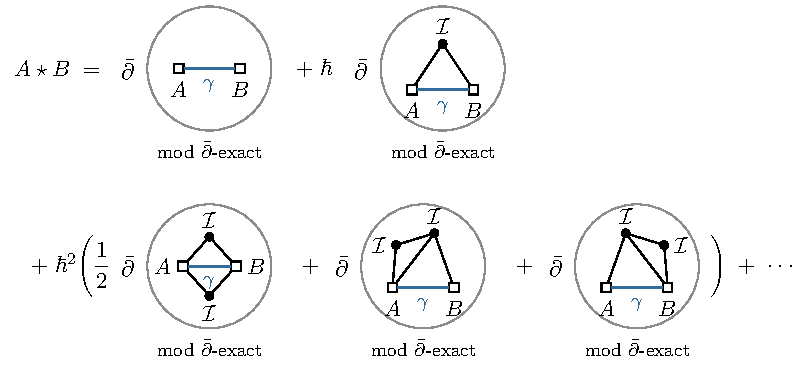
\includegraphics[width=\linewidth]{figures/circuits/product_graphs.pdf}
\caption{The quantum product \eqref{eq:star} through order $\hbar^2$: the free differential $\bar\partial$ acting on the marked graphs, as in Figure~\ref{fig:Q-graphs}. Squares are the insertions $A$ and $B$, dots the interaction vertices $\mathcal I$. The blue edge $\gamma$ is the propagator of the pair $a,b_{\mathrm{aux}}$ in \eqref{eq:1.3}, which acts as the integration contour of \eqref{eq:ring-normal-ordering}; at order zero $\bar\partial$ turns it into the heat kernel and gives $AB$ \eqref{eq:1.4}. Black edges contract fields of $\mathcal I$, $A$ and $B$. Each coefficient is $\hbar^n/n!$ times the number of labellings of the interaction vertices.}
\label{fig:product-graphs}
\end{figure}

The quantum product is
\begin{equation}\label{eq:star}
A\star B=\sum_{n\ge0}\frac{\hbar^n}{n!}
\{\mathcal I^{\otimes n},A,B\}^{\gamma,0}.
\end{equation}

The higher brackets satisfy quadratic identities \cite[Section 3.2]{operatope}, proved for all graph integrals in \cite[Theorem 7]{Wang}; Appendix~\ref{sec:B-short-circuits} gives the proof in network language. They give the $L_\infty$ relations of the brackets \cite[Section 3.5]{higher}, \cite[Remark 14]{Wang}, a higher form of the Jacobi identity \cite[Equation (4.42)]{higher}, that is, of the Leibniz rule; with one marked entry they give the Leibniz rule of $\mathbf Q$ for the quantum product (Section~\ref{sec:dressed-chain}). In them the marked edge acts as an integration contour, as for the regularized product of a chiral algebra \cite[Equations (4.38)--(4.39)]{higher} and the Bochner--Martinelli form of the four-dimensional bracket \cite[Equations (4.40)--(4.41)]{higher}: the contraction of $a(x)$ with $b_{\mathrm{aux}}(0)$ is the propagator form, and the quantum product takes the contour form
\begin{equation}\label{eq:ring-normal-ordering}
\int_{S^3}\Omega\wedge
\underbrace{[P_{0,\infty}(x)]_\Omega}_{\substack{\text{contraction of}\\ a(x)\text{ with }b_{\mathrm{aux}}(0)}}\,
\underbrace{(A(x)B(0))[L]}_{\substack{\text{renormalized two-}\\\text{insertion expansion}}},
\end{equation}
where $S^3$ surrounds the origin and avoids all other insertions. This is the quantum normal-ordering product of \cite[Section 2.3 and footnote 28]{semichiral}. At order zero, $\int_{S^3}\Omega\wedge[P_{0,\infty}]_\Omega=1$ \eqref{eq:ring-propagator-residue} reproduces \eqref{eq:1.4}. Section~\ref{sec:normal-ordering} shows that the class of \eqref{eq:ring-normal-ordering} does not depend on the sphere, and Theorem~\ref{thm:normal-ordering} proves that it is the class of \eqref{eq:star} at every order.

\begin{proposition}[Edge counts of the product graphs]\label{prop:product-counts}
Let $\Gamma$ be a nonzero connected marked graph of \eqref{eq:star} at order $\hbar^n$, $n\ge1$. It has $n$ interaction vertices, the two insertions $A,B$, and $2n+1$ edges: the auxiliary edge $AB$, which contributes its kernel, and $2n$ edges contracting fields in $\mathcal I$, $A$ and $B$. Removing $A$ and $B$ leaves the interaction subgraph (Figure~\ref{fig:forests}). For one of its components $T_j$, with $|T_j|$ vertices, $I_j$ denotes its internal edges and $E_j$ its edges to $A$ or $B$, the spokes. Every edge other than $AB$ is an internal edge or a spoke of exactly one component, and
\begin{equation}\label{eq:1.20}
|T_j|-1\;\le\;|I_j|\;\le\;|T_j|-\#(\bar W\text{ vertices in }T_j),\qquad
|I_j|+|E_j|=2|T_j|.
\end{equation}
\end{proposition}
\begin{proof}
In the circuit of $\Gamma$ (Remark~\ref{rem:circuit}) every edge is a resistor, and the marked resistor joins the insertions $A$ and $B$.

\emph{Internal resistors.} The $|T_j|$ nodes of $T_j$ are connected through its internal resistors. Every resistor joins an antifield terminal to a field terminal (Lemma~\ref{lem:antifield}); an internal resistor of $T_j$ takes its antifield terminal from a node of $T_j$, and a gauge or matter node supplies one antifield terminal, a $\bar W$ node none:
\[
\underbrace{|T_j|-1}_{T_j\text{ connected}}
\;\le\;|I_j|\;\le\;
\underbrace{|T_j|-\#(\bar W\text{ vertices in }T_j)}_{\text{antifield terminals in }T_j}.
\]

\emph{Resistors at the insertions.} A physical resistor between $A$ and $B$ would be in parallel with the marked resistor (Theorem~\ref{thm:no-parallel}). Every physical resistor therefore ends at an interaction node, and it is an internal resistor or a spoke of the component of that node. Summing over the components,
\begin{equation}\label{eq:product-edge-sum}
\sum_j\bigl(|I_j|+|E_j|\bigr)=2n=2\sum_j|T_j|.
\end{equation}

\emph{Ohm's law on $T_j\cup\{A,B\}$.} The subcircuit formed by the nodes of $T_j$, the two insertions and the marked resistor obeys the local count of Ohm's law (Theorem~\ref{thm:laman-subgraph}):
\[
\begin{aligned}
&|I_j|+|E_j|+\underbrace{1}_{AB}\;\le\;2(|T_j|+2)-3\\
\Longrightarrow\quad&|I_j|+|E_j|\;\le\;2|T_j|.
\end{aligned}
\]
By \eqref{eq:product-edge-sum}, equality holds for every component.
\end{proof}

\begin{figure}[H]
\centering
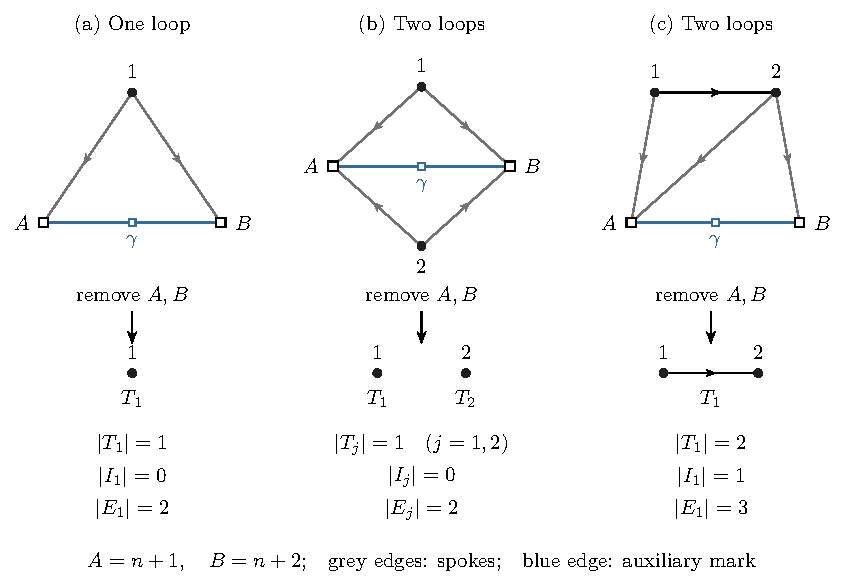
\includegraphics[width=0.9\linewidth,height=.70\textheight,keepaspectratio]{figures/circuits/product_forest.pdf}
\caption{Marked graph topologies through two loops and their internal forests. The squares $A=n+1$ and $B=n+2$ are the two operator insertions; the blue edge carries the auxiliary mark $\gamma$. Deleting $A,B$ and all incident edges leaves (a) one isolated vertex, (b) two isolated vertices, and (c) a two-vertex tree. The black edge is internal; the grey edges are spokes to the insertions. The displayed spoke counts refer to the full graphs in the top row.}
\label{fig:forests}
\end{figure}

\begin{proposition}[Graphs of the quantum product]\label{prop:product-forest}
For the interaction \eqref{eq:B.10}, with $\bar W$ of any degree, let $\Gamma$ be a nonzero connected marked graph of \eqref{eq:star} at order $\hbar^n$, $n\ge1$. Then
\begin{equation}\label{eq:1.19}
\Gamma\setminus\{A,B\}=\coprod_jT_j,\qquad T_j\text{ a tree},\qquad
\#(\bar W\text{ vertices in }T_j)\leq1,\qquad
|E_j|=|T_j|+1.
\end{equation}
Every $T_j$ is joined to both $A$ and $B$, every interaction vertex has degree at least two, and loop diagrams contain no quadratic term of the superpotential $\bar W$.
\end{proposition}
\begin{figure}[H]
\centering
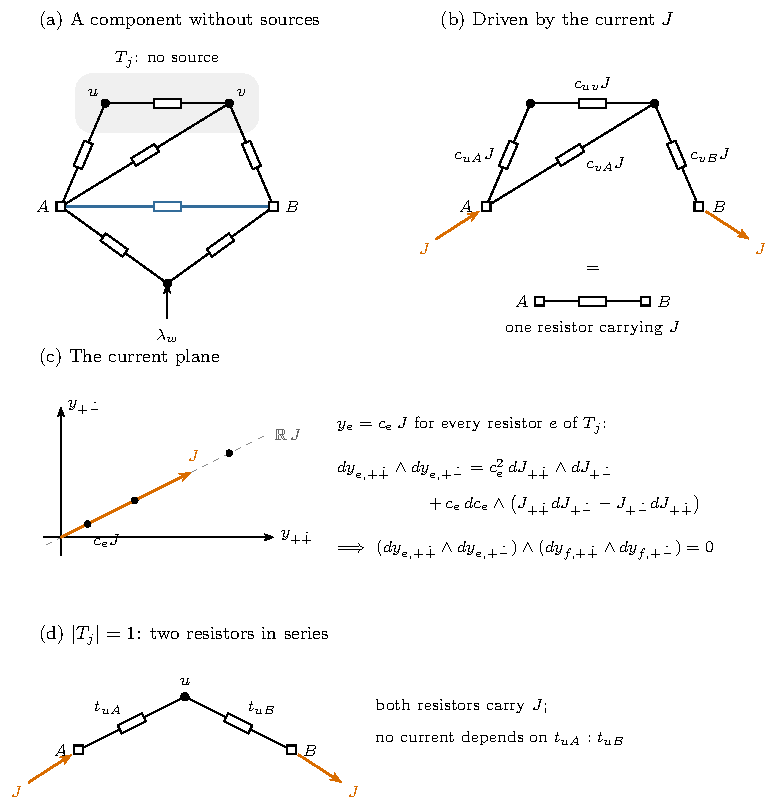
\includegraphics[width=0.86\linewidth,height=.62\textheight,keepaspectratio]{figures/circuits/sourceless_component.pdf}
\caption{A component without sources. (a) A component $T_j$ with no injected current meets the rest of the circuit only at the insertions $A$ and $B$; here the rest is the marked resistor (blue) and a node fed by $\lambda_w$. (b) The current $J$ entering $T_j$ at $A$ leaves it at $B$, and every current of $T_j$ is $c_eJ$ with a real current-division ratio $c_e$: the component acts as one resistor carrying $J$. (c) All currents of $T_j$ lie on the line $\mathbb RJ$ of the current plane, so each of their area forms is \eqref{eq:sourceless-component}, and the product of two of them vanishes. (d) For $|T_j|=1$ the two resistors are in series, and no current depends on the ratio of their resistances.}
\label{fig:sourceless}
\end{figure}

\begin{proof}
In the circuit of $\Gamma$ (Remark~\ref{rem:circuit}) the interaction vertices are nodes and the edges resistors, and an output field left at a node injects a current there.

\emph{Components without sources.} Suppose that no current is injected at the nodes of $T_j$ (Figure~\ref{fig:sourceless}(a)). The component touches the rest of the circuit only at the insertions $A$ and $B$, so the current $J$ that enters it at $A$ leaves it at $B$, and inside it Kirchhoff's laws are those of a passive network driven by $J$. Every current of the component is therefore a real multiple $c_eJ$ of $J$, with a current-division ratio $c_e$ fixed by its resistances: the component acts as one resistor carrying $J$ (Figure~\ref{fig:sourceless}(b)). As the resistances vary, its currents move along the single direction of $J$ in the current plane (Figure~\ref{fig:sourceless}(c)):
\begin{equation}\label{eq:sourceless-component}
dy_{e,+\dot+}\wedge dy_{e,+\dot-}
=c_e^2\,dJ_{+\dot+}\wedge dJ_{+\dot-}
+c_e\,dc_e\wedge\bigl(J_{+\dot+}dJ_{+\dot-}-J_{+\dot-}dJ_{+\dot+}\bigr).
\end{equation}
Both terms contain the two-form $dJ_{+\dot+}\wedge dJ_{+\dot-}$ or the one-form $J_{+\dot+}dJ_{+\dot-}-J_{+\dot-}dJ_{+\dot+}$, so the product of two such factors vanishes. The component brings $|T_j|$ nodes and $2|T_j|$ resistors (Proposition~\ref{prop:product-counts}), hence $|T_j|$ independent loop currents, and the current form \eqref{eq:operatope} contains one factor \eqref{eq:sourceless-component} for each of them. For $|T_j|\ge2$ the form vanishes. For $|T_j|=1$ the single node is joined to $A$ and $B$ by two resistors in series, both carrying $J$; no current depends on the ratio of their resistances, and the form vanishes (Figure~\ref{fig:sourceless}(d)).

\emph{Trees.} If the internal resistors of $T_j$ close a loop, they number at least $|T_j|$; by \eqref{eq:1.20} they number exactly $|T_j|$, $T_j$ has no $\bar W$ node, and $|E_j|=|T_j|$. The $2|T_j|$ ends of the internal resistors and the $|T_j|$ spokes then wire all $3|T_j|$ terminals of its cubic nodes. No current is injected in $T_j$, and the first step gives zero. Every $T_j$ is therefore a tree, $|I_j|=|T_j|-1$, and \eqref{eq:1.20} gives at most one $\bar W$ node and $|E_j|=|T_j|+1$, which is \eqref{eq:1.19}.

\emph{Spokes and degrees.} Two resistors between the same two nodes are in parallel and give zero (Theorem~\ref{thm:no-parallel}), so a node has at most one spoke to $A$ and one to $B$. Each insertion therefore receives at most $|T_j|$ of the $|T_j|+1$ spokes of $T_j$, and both receive at least one. A node wired by a single resistor would be a dead end: that resistor carries exactly the current injected at the node, whatever its resistance, so its resistance moves no current and the current form vanishes. Every interaction node therefore has at least two resistors.

\emph{Quadratic terms of $\bar W$.} A quadratic term of $\bar W$ is a node with two terminals, both wired by the previous step, so it injects no current. It is the only $\bar W$ node of its tree, whose $3(|T_j|-1)+2=3|T_j|-1$ terminals are then all wired by the $|T_j|-1$ internal resistors and the $|T_j|+1$ spokes. The tree carries no source, and the first step gives zero.
\end{proof}


\begin{proposition}[Cubic interactions]\label{prop:product-cubic}
Let every vertex of $\mathcal I$ be cubic, as are the gauge and matter vertices of \eqref{eq:B.10} together with a cubic $\bar W$. In every tree $T_j$ of \eqref{eq:1.19}, exactly one vertex has degree two, and its uncontracted field is the only output field of $T_j$; all other vertices have degree three. The tree degree of a vertex is its number of internal edges, and the number of spokes at a vertex of given tree degree is
\begin{equation}\label{eq:product-local-spokes}
\begin{array}{c|cccc}
\text{tree degree}&0&1&2&3\\\hline
\text{spokes at a degree-three vertex}&\text{--}&2&1&0\\
\text{spokes at the degree-two vertex}&2&1&0&\text{--}
\end{array}
\end{equation}
and a vertex with two spokes is joined to both $A$ and $B$ (Figure~\ref{fig:forest-components}). Conversely, the edge $AB$, a forest of trees, and spokes obeying \eqref{eq:product-local-spokes}, with one degree-two vertex in each tree, form a graph satisfying \eqref{eq:1.11}.
\end{proposition}
\begin{figure}[H]
\centering
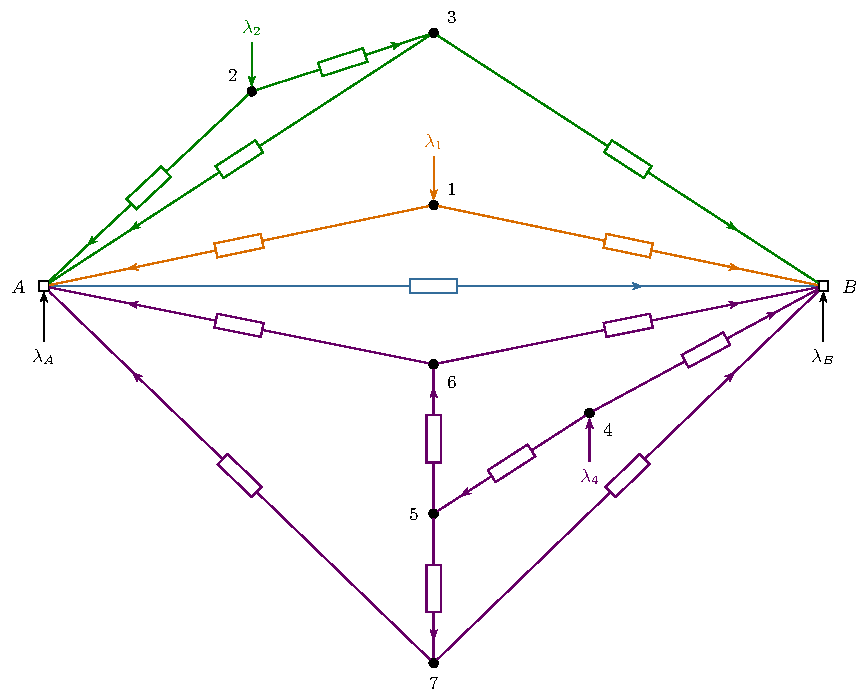
\includegraphics[width=0.9\linewidth,height=.60\textheight,keepaspectratio]{figures/circuits/forest_components.pdf}
\caption{A seven-loop product graph with three trees, each in its own colour, between the insertions $A$ and $B$; the marked edge $AB$ is blue. Each tree has one more spoke than vertices, and its source enters at its only vertex of degree two: $1$, $2$ and $4$. Leaves of degree three are joined to both insertions, and the branching vertex $5$ has no spoke.}
\label{fig:forest-components}
\end{figure}

\begin{proof}
A cubic node has three terminals. In $T_j$ the $|T_j|-1$ internal resistors wire $2(|T_j|-1)$ terminals and the $|T_j|+1$ spokes wire $|T_j|+1$ more, so the numbers of resistors at its nodes add up to
\begin{equation}\label{eq:product-degree-sum}
\sum_{v\in T_j}\deg_\Gamma v=2(|T_j|-1)+(|T_j|+1)=3|T_j|-1 .
\end{equation}
Every node has two or three resistors by Proposition~\ref{prop:product-forest}, so exactly one node has two, and
\begin{equation}\label{eq:1.21}
\underbrace{3|T_j|}_{\text{terminals}}-\underbrace{2(|T_j|-1)}_{\text{internal resistor ends}}-\underbrace{(|T_j|+1)}_{\text{spokes}}=1
\end{equation}
terminal stays free, at that node: each tree carries a single source, injected at its node with two resistors. A node has at most one spoke to each insertion, and its spokes are its resistors other than its internal ones; this gives \eqref{eq:product-local-spokes}.

For the converse, the local count of Ohm's law (Theorem~\ref{thm:laman-subgraph}) is checked on every subcircuit. A subtree $P$ of $T_j$ with $k$ internal resistors leaving it sends
\begin{equation*}
\sum_{v\in P}\deg_\Gamma v-2(|P|-1)-k\le|P|+2-k
\end{equation*}
spokes to the insertions, at most $|P|+1$ for $P\ne T_j$. A subcircuit on a node set $S$ with $|S|\ge2$ meets the trees in subtrees $P_1,\ldots,P_m$. If it contains $A$ and $B$, it has at most $\sum_i2|P_i|+1=2|S|-3$ resistors, the marked one included. If it contains one insertion, each of its nodes has at most one spoke to it, and it has at most $\sum_i(2|P_i|-1)\le2|S|-3$ resistors. Otherwise its resistors form no loop, and they number at most $|S|-1\le2|S|-3$. Together with $|\Gamma_1|=2n+1$ this is \eqref{eq:1.11}.
\end{proof}
\subsection{Spiders}
\label{sec:spiders}

A superpotential vertex of degree greater than three can join several arms (Proposition~\ref{prop:superpotential-spider}).

\begin{definition}[Spiders and books]\label{def:spiders-books}
A \emph{spider} consists of paths meeting only at a vertex $A$, together with a second vertex $B$ joined to every vertex of these paths, including $A$. In the supercharge graphs, $A$ carries $\bar W$ and $B=\mathcal O$. The $i$th arm contains $\ell_i$ cubic vertices, labelled $v_{i,1},\ldots,v_{i,\ell_i}$ from its outer end towards $A$; its length is $\ell_i$ and the loop number is $n=\sum_i\ell_i$.

A \emph{book} is the case $\ell_i=1$ for every arm. Its $n$ triangles $A v_{i,1} B$ share the edge $AB$, and each triangle is a page. At one loop both families give the triangle. Figure~\ref{fig:spider} shows the one-loop triangle, the first extended arm and the first two-page book.
\end{definition}

\begin{figure}[H]
\centering
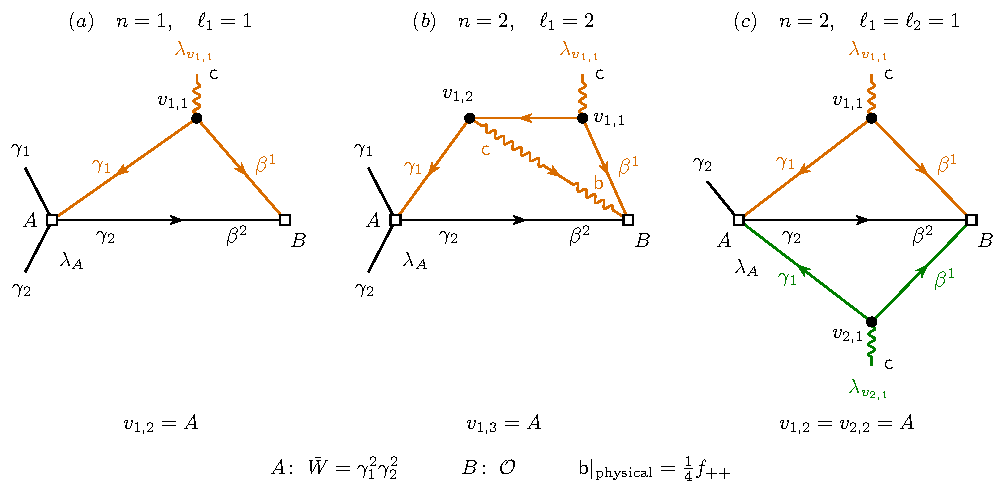
\includegraphics[width=0.98\linewidth,height=.70\textheight,keepaspectratio]{figures/circuits/spider_general_coloured.pdf}
\caption{One- and two-loop spiders for $\bar W=\gamma_1^2\gamma_2^2$: (a) $\ell_1=1$; (b) $\ell_1=2$; (c) $\ell_1=\ell_2=1$. The superpotential vertex is $A$ and the operator insertion is $B$; each arm, with its spokes, has its own colour. Arm indices increase towards $A=v_{i,\ell_i+1}$. Each $v_{i,1}$ carries an output $\mathsf c$; the output matter at $A$ supplies $\lambda_A$.}
\label{fig:spider}
\end{figure}

On arm $i$, $v_{i,1}$ carries the source, $v_{i,\ell_i}$ is adjacent to $A$, and $v_{i,\ell_i+1}=A$. The remaining arm vertices are fully contracted:
\begin{equation}\label{eq:1.47}
\begin{gathered}
\Gamma_1=\big((v_{i,j},v_{i,j+1}),(v_{i,j},B)\big)_{i=1,\ldots,a;\ j=1,\ldots,\ell_i}
\cup\{(A,B)\},\\
\ell_1+\cdots+\ell_a=n,\qquad
\lambda_{v_{i,j},+\dot a}=\delta_{j1}\lambda_{v_{i,1},+\dot a}.
\end{gathered}
\end{equation}

Each arm is reduced as a fan is, from its outer end (Figure~\ref{fig:spider-reduction}). Eliminating $v_{i,j}$ combines its two resistors towards $v_{i,j+1}$ and $B$ in series and merges the new branch in parallel with the next spoke; at the last arm vertex the new branch lies across $AB$. Each merge lowers the loop number by one, and only series and parallel moves occur. When every arm is reduced, its branch and the original edge $AB$ merge into one resistor, whose Schwinger time is fixed to one. Appendix~\ref{sec:spider-reduction} derives the resulting chart of edge Schwinger times \eqref{eq:1.49}, with coordinates
\begin{equation}\label{eq:spiderdomain}
0<r_{i,j}<1\quad(j<2\ell_i),\qquad
r_{i,2\ell_i}>0,\qquad\sum_i r_{i,2\ell_i}<1.
\end{equation}
Here $r_{i,2j-1}$ is the fraction of the source at $v_{i,j}$, after the earlier eliminations, that the series step passes to $v_{i,j+1}$, the rest going to $B$; for $j<\ell_i$, $r_{i,2j}$ is the fraction of the merged spoke current at $v_{i,j+1}$ carried by the new branch; and $r_{i,2\ell_i}$ is the fraction of the final current carried by the branch of arm $i$, the original edge $AB$ carrying $1-\sum_ir_{i,2\ell_i}$. The final resistor carries the reduced current $y^{\mathrm{red}}_{AB}$, which by conservation at $A$ is the source collected at $A$: $\lambda_A$ and, from each arm, the fraction of its source passed along the whole arm,
\begin{equation}\label{eq:spider-reduced}
y^{\mathrm{red}}_{AB,+\dot a}
=\lambda_{A,+\dot a}+\sum_i
\left(\prod_{k=1}^{\ell_i}r_{i,2k-1}\right)\lambda_{v_{i,1},+\dot a}.
\end{equation}
Reversing the reductions splits $y^{\mathrm{red}}_{AB}$ back into the original currents \eqref{eq:1.50}--\eqref{eq:1.51}.

\begin{figure}[H]
\centering
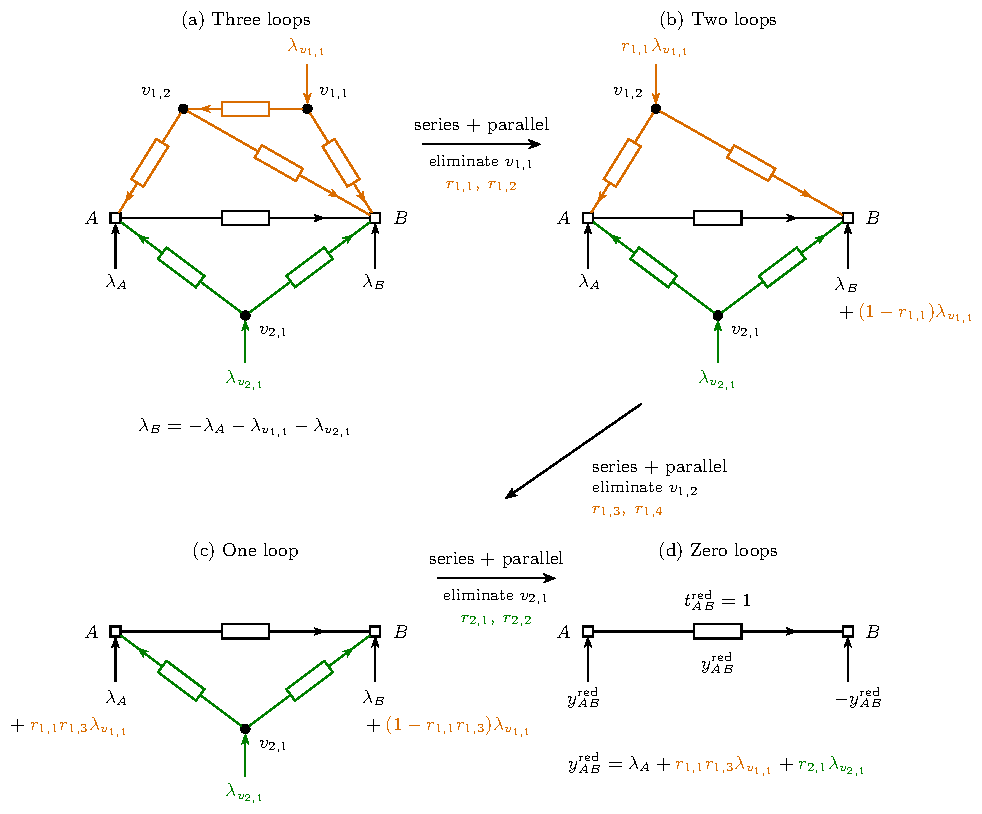
\includegraphics[width=0.98\linewidth,height=.70\textheight,keepaspectratio]{figures/circuits/spider_reduction.pdf}
\caption{Reduction of the three-loop spider with arms $\ell_1=2$ (orange) and $\ell_2=1$ (green). Each step eliminates an arm vertex by a series step, which passes the fraction $r_{i,2j-1}$ of its source along the arm and the rest to $B$, and a parallel merge with the next spoke or with $AB$; each step lowers the loop number by one. The last panel is the unit resistor carrying \eqref{eq:spider-reduced}.}
\label{fig:spider-reduction}
\end{figure}

Appendix~\ref{sec:spider-jacobian} computes the current Jacobian in these coordinates as for the fan: it is block lower triangular, with one two-by-two block for each interior elimination and one block for the final parallel merge,
\begin{equation}\label{eq:1.53}
\begin{aligned}
\mathcal I_\Gamma^{\mathrm{raw\ cut}}(\lambda;z)
={}&\int_{\eqref{eq:spiderdomain}}\prod_{i=1}^a\prod_{j=1}^{2\ell_i}dr_{i,j}\,
\underbrace{\left(1-\sum_i r_{i,2\ell_i}\right)}_{\text{final parallel merge}}\\
&\times\prod_{i=1}^a\,
\underbrace{r_{i,2\ell_i}^{\ell_i-1}\prod_{j=1}^{\ell_i-1}\Big[r_{i,2j-1}^{\ell_i-j}\,r_{i,2j}^{\,j-1}\,(1-r_{i,2j})\Big]
\bigl[\lambda_{v_{i,1},+\dot a}y^{\mathrm{red}}_{AB,+}{}^{\dot a}\bigr]^{\ell_i}}_{\text{diagonal blocks of arm }i}
\,e^{-\sum_e y_{e,+\dot a}(r)z_e^{+\dot a}}.
\end{aligned}
\end{equation}

The cubic arm vertices carry no derivatives, so $z_{v_{i,j}v_{i,j+1}}=0$ for $j<\ell_i$; the spokes, the last arm edges and $AB$ keep general displacements. The exponential then translates the outputs at $v_{i,1}$ and $A$:
\begin{equation}\label{eq:spider-output-translation}
-\sum_e y_{e,+\dot a}(r)z_e^{+\dot a}
=\lambda_{A,+\dot a}x_A^{+\dot a}(r,z)
+\sum_{i=1}^a\lambda_{v_{i,1},+\dot a}x_{v_{i,1}}^{+\dot a}(r,z),
\end{equation}
with translated positions
\begin{equation}\label{eq:spider-output-points}
\begin{aligned}
x_A^{+\dot a}(r,z)
={}&-\left(1-\sum_i r_{i,2\ell_i}\right)z_{AB}^{+\dot a}\\
&-\sum_{i=1}^a r_{i,2\ell_i}\left[
\sum_{j=1}^{\ell_i}(1-r_{i,2j-2})
\left(\prod_{k=j}^{\ell_i-1}r_{i,2k}\right)z_{v_{i,j}B}^{+\dot a}
-z_{v_{i,\ell_i}A}^{+\dot a}\right],\\[3pt]
x_{v_{i,1}}^{+\dot a}(r,z)
={}&-\sum_{s=1}^{\ell_i}(1-r_{i,2s-1})
\left(\prod_{k=1}^{s-1}r_{i,2k-1}\right)
\sum_{j=1}^{s}(1-r_{i,2j-2})
\left(\prod_{k=j}^{s-1}r_{i,2k}\right)z_{v_{i,j}B}^{+\dot a}\\
&+\left(\prod_{k=1}^{\ell_i}r_{i,2k-1}\right)
\bigl(x_A^{+\dot a}(r,z)-z_{v_{i,\ell_i}A}^{+\dot a}\bigr),
\qquad r_{i,0}=0.
\end{aligned}
\end{equation}

For nonnegative integers $\kappa_{i,j}$ and $\bar\kappa_{i,2j}$, the weighted monomial moments on \eqref{eq:spiderdomain} are
\begin{equation}\label{eq:spider-moments}
\begin{aligned}
&\int_{\eqref{eq:spiderdomain}}\prod_{i,j}dr_{i,j}
\left(1-\sum_i r_{i,2\ell_i}\right)
\prod_{i=1}^a\Bigg[r_{i,2\ell_i}^{\ell_i-1+\kappa_{i,2\ell_i}}
\prod_{j=1}^{\ell_i}r_{i,2j-1}^{\ell_i-j+\kappa_{i,2j-1}}
\prod_{j=1}^{\ell_i-1}r_{i,2j}^{j-1+\kappa_{i,2j}}(1-r_{i,2j})^{1+\bar\kappa_{i,2j}}\Bigg]\\
&=\frac{\prod_i(\ell_i-1+\kappa_{i,2\ell_i})!}{(n+1+\sum_i \kappa_{i,2\ell_i})!}
\prod_{i=1}^a\Bigg[\prod_{j=1}^{\ell_i}\frac1{\ell_i-j+1+\kappa_{i,2j-1}}
\prod_{j=1}^{\ell_i-1}
\frac{(j-1+\kappa_{i,2j})!\,(1+\bar\kappa_{i,2j})!}{(j+1+\kappa_{i,2j}+\bar\kappa_{i,2j})!}\Bigg].
\end{aligned}
\end{equation}

The exponent is reduced by \eqref{eq:spider-loop-split} and \eqref{eq:spider-arm-current}. Sum over nonnegative integers $m_{iA}$, $m_{ik}$ $(k\ne i)$ with $m_{iA}+\sum_{k\ne i}m_{ik}=\ell_i$, $p_{ijs}$ $(1\le j\le s\le\ell_i)$, and $q_{ijA}$, $q_{ijk}$ $(1\le j\le\ell_i,\ 1\le k\le a)$, and write $q_{ij}=q_{ijA}+\sum_kq_{ijk}$ and $M_i=\sum_{k\ne i}m_{ki}+\sum_{k=1}^a\sum_{j=1}^{\ell_k}q_{kji}$. For arbitrary edge displacements, with $v_{i,\ell_i+1}=A$, the full Taylor expansion is
\begin{equation}\label{eq:spider-full-taylor}
\begin{aligned}
&\mathcal I_\Gamma^{\mathrm{raw\ cut}}(\lambda;z)
=e^{-\lambda_{A,+\dot a}z_{AB}^{+\dot a}
-\sum_i\lambda_{v_{i,1},+\dot a}z_{v_{i,1}B}^{+\dot a}}
\sum_{m,p,q}\prod_{i=1}^a\Bigg\{\\
&\quad\hphantom{{}\times{}}\ell_i!\,
\frac{(\lambda_{v_{i,1},+\dot b}\lambda_{A,+}{}^{\dot b})^{m_{iA}}}{m_{iA}!}
\prod_{k\ne i}
\frac{(\lambda_{v_{i,1},+\dot c}\lambda_{v_{k,1},+}{}^{\dot c})^{m_{ik}}}{m_{ik}!}\\
&\quad\times\prod_{j=1}^{\ell_i}\Bigg[
\prod_{s=j}^{\ell_i}
\frac{\bigl[-\lambda_{v_{i,1},+\dot d}
(z_{v_{i,j}v_{i,j+1}}+z_{v_{i,j+1}B}-z_{v_{i,j}B})^{+\dot d}\bigr]^{p_{ijs}}}{p_{ijs}!}\\
&\qquad\times
\frac{\bigl[\lambda_{A,+\dot e}
(z_{v_{i,j}v_{i,j+1}}+z_{v_{i,j+1}B}-z_{v_{i,j}B})^{+\dot e}\bigr]^{q_{ijA}}}{q_{ijA}!}\\
&\qquad\times\prod_{k=1}^a
\frac{\bigl[\lambda_{v_{k,1},+\dot f}
(z_{v_{i,j}v_{i,j+1}}+z_{v_{i,j+1}B}-z_{v_{i,j}B})^{+\dot f}\bigr]^{q_{ijk}}}{q_{ijk}!}
\Bigg]\Bigg\}\\
&\quad\times
\frac{\prod_i\left(\ell_i-1+\sum_{j}q_{ij}\right)!}
{\left(n+1+\sum_{i,j}q_{ij}\right)!}
\prod_{i=1}^a\prod_{t=1}^{\ell_i}
\frac1{\ell_i-t+1+M_i+\sum_{s=t}^{\ell_i}\sum_{j=1}^{s}p_{ijs}}\\
&\quad\times\prod_{i=1}^a\prod_{t=1}^{\ell_i-1}
\frac{\left(t-1+\sum_{j=1}^{t}\left[q_{ij}+\sum_{s=t+1}^{\ell_i}p_{ijs}\right]\right)!\,
\left(1+\sum_{j=1}^{t}p_{ijt}\right)!}
{\left(t+1+\sum_{j=1}^{t}\left[q_{ij}+\sum_{s=t}^{\ell_i}p_{ijs}\right]\right)!}.
\end{aligned}
\end{equation}
For the physical displacements, $z_{v_{i,j}v_{i,j+1}}=0$ for $j<\ell_i$. Taking one arm gives the Taylor coefficients of \eqref{eq:fan-full-taylor}, and taking every arm to have length one gives the book kernel \eqref{eq:B-book-full-kernel} of Appendix~\ref{sec:book-jacobian}, whose one- and two-loop values agree with \cite[Equations (4.20) and (4.44)]{operatope} and \cite[Equations (4.2) and (0.5)]{GWW}.

\subsection{Kernels of general product forests}
\label{sec:forest-graphs}

Spiders do not exhaust the graphs of the quantum product: other graphs occur from three loops on and are the majority from four loops on, where the trees also begin to branch (Table~\ref{tab:product-census}). The moves of Appendix~\ref{sec:B-kernel-recursion} reduce all of them.\footnote{From three loops on, some of these graphs are Laman graphs not of type~I$'$ \cite[Definition 4.12]{GWW}: in the three-loop graph with edges $12,13,2A,2B,3A,3B,AB$, the only degree-two vertex, $1$, has neighbours that are not joined. These reductions therefore reach beyond the recursion of \cite[Theorem 4.13]{GWW}.}

\begin{proposition}[Kernels of cubic product forests]\label{prop:forest-kernels}
Let $\Gamma$ be a nonzero marked graph of the quantum product with cubic interaction vertices (Proposition~\ref{prop:product-cubic}), and root each tree at its vertex of degree two, its only source. The subtree of a vertex consists of the vertices whose path to the root passes through it.
\begin{enumerate}
\item[(i)] If $\Gamma$ is of type~I$'$, series--parallel moves (Theorem~\ref{thm:kernel-series-parallel}) along each arm reduce it to the marked resistor, which then carries
\begin{equation}\label{eq:product-typeI-current}
y^{\mathrm{red}}_{AB,+\dot a}
=\lambda_{A,+\dot a}
+\sum_{\text{arms at }B}\left(\prod_{k=1}^{\ell_i}r_{i,2k-1}\right)\lambda_{v_{i,1},+\dot a}
+\sum_{\text{arms at }A}\left(1-\prod_{k=1}^{\ell_i}r_{i,2k-1}\right)\lambda_{v_{i,1},+\dot a}.
\end{equation}
summed over the arms wired to $B$ and to $A$.
\item[(ii)] Every $\Gamma$ is reduced to the marked resistor by removing each vertex after all the vertices of its subtree. A source-free vertex is removed by a star--triangle move (Theorem~\ref{thm:kernel-star-triangle}) when its tree neighbour towards the root has a spoke, and together with its sibling (Theorem~\ref{thm:kernel-two-leaves}) when that neighbour has none; the root is removed last, by a series--parallel move.
\item[(iii)] The kernel of $\Gamma$ is an integral over $2n$ coordinates, ranging over intervals and simplices, of a polynomial density times the exponential of polynomial currents, and each Taylor coefficient in the displacements is a finite sum of the moments \eqref{eq:Dirichlet}.
\end{enumerate}
\end{proposition}
\begin{proof}
(i) By Proposition~\ref{prop:product-spider}(ii), every tree is an arm $v_{i,1}-\cdots-v_{i,\ell_i}$ whose nodes are all wired to one insertion, with the source at $v_{i,1}$ and a resistor from $v_{i,\ell_i}$ to each insertion. On an arm wired to $B$, the two resistors of $v_{i,1}$ end at $v_{i,2}$ and $B$, which are joined, so Theorem~\ref{thm:kernel-series-parallel} removes $v_{i,1}$ and passes the fraction $r_{i,1}$ of its source to $v_{i,2}$, which then has two resistors in turn. The source that reaches the last node of the arm is $\prod_kr_{i,2k-1}\lambda_{v_{i,1}}$, and the last move passes it to $A$ across the marked resistor, as for the spider \eqref{eq:spider-reduced}. On an arm wired to $A$ the same moves run with $A$ and $B$ exchanged, and the fraction of the source that reaches $A$ is $1-\prod_kr_{i,2k-1}$. Conservation at $A$ gives \eqref{eq:product-typeI-current}.

(ii) A source-free vertex $v$ whose subtree is gone has three resistors, to its tree neighbour $u$ towards the root, to $A$ and to $B$: its own spokes and the sides left by the moves at its children, merged in parallel. If $u$ has a spoke, to $X\in\{A,B\}$, two sides of the triangle that replaces $v$, namely $uX$ and $AB$, merge with resistors already there, and Theorem~\ref{thm:kernel-star-triangle} removes $v$. If $u$ has none, then by \eqref{eq:product-local-spokes} $u$ has a second child $v'$, and once the subtree of $v'$ is gone, Theorem~\ref{thm:kernel-two-leaves} removes $v$ and $v'$ together. In both cases $u$ is then wired to $A$ and to $B$. The root, once its subtree is gone, has two resistors, to $A$ and to $B$, which the marked resistor joins, and Theorem~\ref{thm:kernel-series-parallel} removes it across $AB$.

(iii) Each move integrates the kernel of the smaller circuit over its ratios with a polynomial factor. The currents of the larger circuit are linear in those of the smaller one with polynomial coefficients, and the series--parallel moves pass sources on with the weights $r_1$ and $1-r_1$. A move removes one loop with two coordinates, or two loops with four, so the coordinates number $2n$. Expanding the exponential, every Taylor coefficient is a polynomial integral over products of intervals and simplices, a finite sum of \eqref{eq:Dirichlet}.
\end{proof}
\begin{figure}[H]
\centering
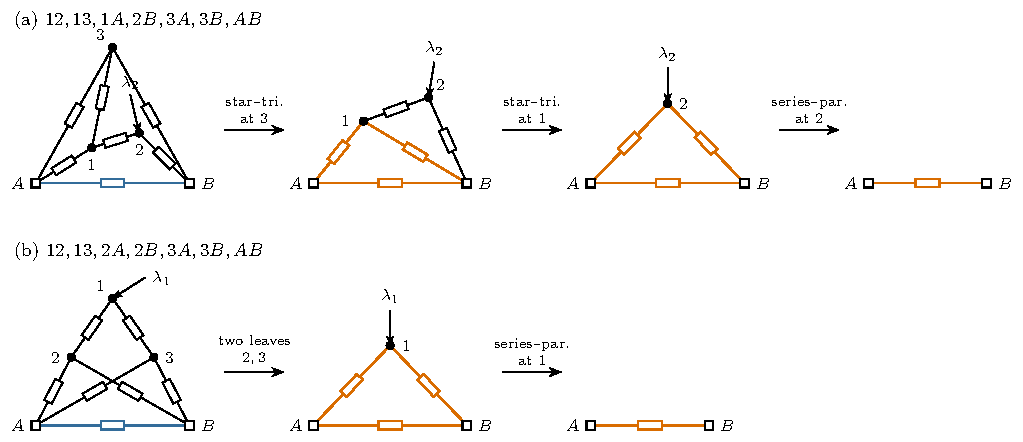
\includegraphics[width=\linewidth]{figures/circuits/forest_three_loop.pdf}
\caption{The two three-loop graphs not of type~I$'$, reduced as in Proposition~\ref{prop:forest-kernels}(ii); orange: the resistors created or merged by the preceding move, blue: the marked resistor. (a) Star--triangle moves (Theorem~\ref{thm:kernel-star-triangle}) at $3$ and at $1$, then a series--parallel move (Theorem~\ref{thm:kernel-series-parallel}) at the root $2$. (b) The leaves $2,3$ hang from the root $1$, which has no spoke, and are removed together (Theorem~\ref{thm:kernel-two-leaves}); the root is removed last.}
\label{fig:forest-three-loop}
\end{figure}

\begin{proposition}[Trees with a superpotential vertex]\label{prop:forest-superpotential}
Let a tree $T_j$ contain one superpotential vertex, with $\deg_\Gamma\bar W$ resistors and $\deg\bar W$ fields, its other vertices being cubic. Then $T_j$ has $\deg_\Gamma\bar W-2$ vertices of degree two, each carrying a source, and the superpotential vertex carries a source when $\deg\bar W>\deg_\Gamma\bar W$. Series--parallel moves pass every source on with the weights $r_1$ and $1-r_1$, so graphs of type~I$'$ keep polynomial currents for any placement of the sources. A star--triangle move at a vertex with a source distributes it with the rational weights \eqref{eq:1.78}, and the currents become rational functions of the coordinates.
\end{proposition}
\begin{proof}
The counts are \eqref{eq:1.23}: the terminals of the cubic nodes and of the superpotential node, minus the ends of the resistors, leave $\deg\bar W-2$ free terminals, $\deg\bar W-\deg_\Gamma\bar W$ of them at the superpotential node and one at each cubic node with two resistors. Theorem~\ref{thm:kernel-series-parallel} holds for any source at the removed node, with the polynomial weights $r_1$ and $1-r_1$. At a star with source $\lambda_v$, the source divides among the three outer nodes in proportion to the opposite sides of the triangle, \eqref{eq:1.78}, and these ratios are rational in the coordinates.
\end{proof}
\begin{example}[Sourced star--triangle moves]\label{ex:sourced-star}
In the graph of Figure~\ref{fig:forest-three-loop}(b), let $2$ be a superpotential vertex with $\deg_\Gamma\bar W=3<\deg\bar W$, so that $1$, $2$, $A$ and $B$ carry sources. The neighbours $2,3$ of the degree-two vertex $1$ are not joined, and the star--triangle move at the only source-free vertex, $3$, merges only the side $AB$. A series step at $1$ and this move each leave the complete circuit on four nodes, all of them with sources, so every elimination order needs a star--triangle move at a vertex with a source. The same holds for the four-loop graph $12,14,23,2A,2B,3A,4A,4B,AB$ with a superpotential vertex $2$ of four resistors, which leaves sources at $1$, $3$, $A$ and $B$. Table~\ref{tab:product-census-general} counts these graphs through seven loops.
\end{example}

\begin{table}[H]
\centering
\begin{tabular}{@{}rrrrrrr@{}}
\toprule
$n$ & graphs & $\bar W$ node with & type~I$'$ & spiders & $\bar W$ node with $\ge4$ & reduced without a\\
 & & $\ge4$ resistors & & & resistors, not type~I$'$ & sourced star--triangle\\
\midrule
3 & 11 & 3 & 8 & 8 & 0 & 0\\
4 & 46 & 23 & 23 & 19 & 10 & 4\\
5 & 200 & 135 & 59 & 37 & 92 & 29\\
6 & 874 & 680 & 152 & 71 & 557 & 144\\
7 & 3765 & 3189 & 370 & 125 & 2864 & 610\\
\bottomrule
\end{tabular}
\caption{Product graphs whose trees have at most one superpotential node, all other nodes cubic, up to isomorphism fixing $A,B$. Columns 3 and 6: superpotential node with at least four resistors; last column: those of column 6 reduced without a sourced star--triangle step.}
\label{tab:product-census-general}
\end{table}

\FloatBarrier
\section{Quantum supercharges and \texorpdfstring{$\mathcal N=4$}{N=4} Yang--Mills theory}
\label{sec:supercharge}

Combining the graph kernels with the BV pairing gives the quantum supercharge. For a general interaction, let $W_\Gamma$ denote the ordered fibre contractions, including their Koszul signs. Restoring the scalar normalization of \eqref{eq:1.7} gives

\begin{equation}\label{eq:2.3}
\begin{aligned}
Q_n\mathcal O
={}&\frac{(-1)^n}{(n+1)!\,(8\pi^2)^n}
\sum_{\substack{\Gamma\ \mathrm{labelled,\ rooted,\ Laman}}}
\Bigl[\mathcal I_\Gamma^{\mathrm{raw\ cut}}(\lambda;z)
W_\Gamma[\mathcal I^{\otimes(n+1)},\mathcal O]\Bigr]
\Big|_{\mathrm{jets},\ z_{v,i}=0}.
\end{aligned}
\end{equation}

Here $n\ge0$ and the root is the insertion. At $n=0$ the single-edge graph gives $Q_0\mathcal O=\{\mathcal I,\mathcal O\}_0$. The fibre derivatives remove the contracted fields from each vertex. The current polynomial then differentiates the fields that remain there, with $\lambda_{v,+\dot a}=\partial/\partial x_v^{+\dot a}$, and these fields are evaluated at the position of $\mathcal O$. A derivative on an input field instead differentiates its edge displacement before that displacement is set to zero. For an input $\mathsf w$, the derivative in $\mathsf w_{\dot a}^A=-\partial\mathsf c^A/\partial x^{+\dot a}$ acts on the edge kernel.

Under $\lambda_{v,+\dot a}\to c\,\lambda_{v,+\dot a}$ and $z_e^{+\dot a}\to z_e^{+\dot a}/c$ at fixed $\dot a$, the displacement exponential in \eqref{eq:operatope} is invariant and the current form, with $n$ factors $dy_{e,+\dot a}$, scales as $c^n$. Since $\lambda_v$ differentiates output fields and each $z_e$-derivative takes a derivative from an input letter, $Q_n$ raises the numbers of $\partial_{+\dot+}$ and $\partial_{+\dot-}$ derivatives by $n$ each, $2n$ in total. An operator with $d_{\dot+}$ and $d_{\dot-}$ holomorphic derivatives is therefore reached by $Q_n$, and by the successive differential $d_n$ of Section~\ref{sec:lifting}, only for $n\le\min(d_{\dot+},d_{\dot-})$, so finitely many orders decide whether it becomes quantum exact.

This section illustrates \eqref{eq:2.3} in familiar theories.

\subsection{The all-order operator}

\begin{figure}[H]
\centering
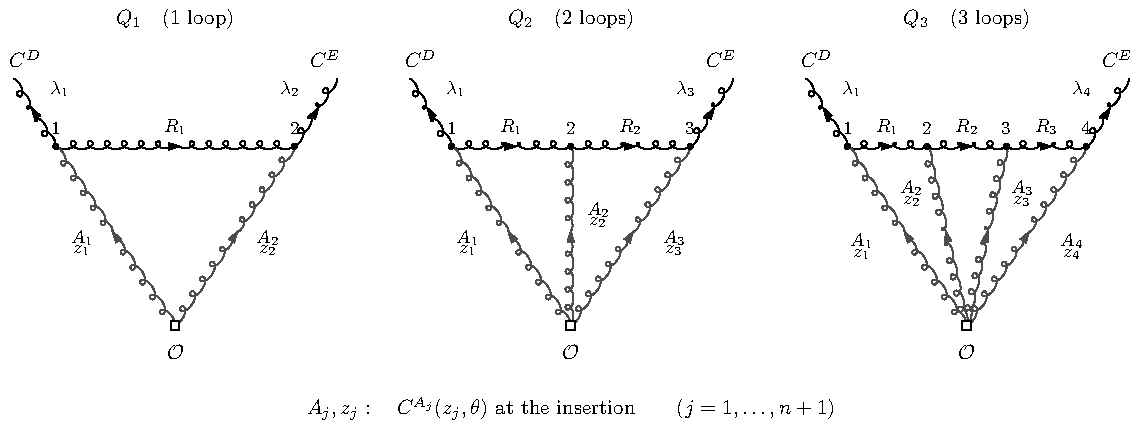
\includegraphics[width=.99\linewidth,height=.70\textheight,keepaspectratio]{figures/n4_three_fans.pdf}
\caption{One-, two- and three-loop supercharge fans in $\mathcal N=4$ Yang--Mills theory. The spoke labelled $A_j,z_j$ contracts an input $C^{A_j}(z_j,\theta)$ at $\mathcal O$. The path contracts the colour indices $R_1,\ldots,R_n$ and leaves the endpoint fields $C^D,C^E$, carrying $\lambda_1,\lambda_{n+1}$.}
\label{fig:n4-supercharge-fans}
\end{figure}
For a fan (Figure~\ref{fig:n4-supercharge-fans}), contracting the cubic vertices of \eqref{eq:A.15} leaves two superfields at the endpoints and a chain of structure constants. The functional derivatives at displaced points are normalized by
\begin{equation}\label{eq:2.10}
\frac{\delta C^B(y,\theta')}{\delta C^A(y',\theta)}=\delta_A{}^B\,\delta^{(4)}(y-y')\prod_{I=1}^3(\theta_I-\theta'_I),
\end{equation}
so that $\int d^4z\,f(z)\,\delta/\delta C^A(x+z,\theta)$ replaces a holomorphic jet $\partial^{m+s}C^A(x,\theta')/\partial(x^{+\dot+})^m\partial(x^{+\dot-})^s$ of an operator at $x$ by the same derivative of $f$ at $z=0$, times the odd delta function.
\Needspace{17\baselineskip}
\begin{theorem}\label{thm:N4-allloop}
For the superfield action \eqref{eq:A.15} and an operator at $x$, the $n$-loop supercharge for $n\ge1$ is
\begin{equation}\label{eq:2.8}
\begin{aligned}
Q_n={}&\frac{(-1)^ni^{n+1}}{2(32\pi^2)^n}
\int_{\eqref{eq:1.37}}dr_1\cdots dr_{2n}\,
\left[\prod_{j=1}^{n-1}r_{2j-1}^{n-j}r_{2j}(1-r_{2j})^{j-1}\right]r_{2n}^{n-1}
\int d^3\theta\int\prod_{j=1}^{n+1}d^4z_j\\
&\times C_{A_1DR_1}
\left(\prod_{j=2}^{n}C_{A_jR_{j-1}R_j}\right)C_{A_{n+1}R_nE}\\
&\times\big(\partial_{+\dot a_1}\cdots\partial_{+\dot a_n}C^D\big)(x+x_1(r,z),\theta)
\big(\partial_+{}^{\dot a_1}\cdots\partial_+{}^{\dot a_n}C^E\big)(x+x_{n+1}(r,z),\theta)\\
&\times\frac{\delta}{\delta C^{A_1}(x+z_1,\theta)}\cdots
\frac{\delta}{\delta C^{A_{n+1}}(x+z_{n+1},\theta)},
\end{aligned}
\end{equation}
where the output fields are differentiated before they are evaluated at the translated positions.
\end{theorem}
The kernel is \eqref{eq:1.41}; the translated positions $x_1(r,z)$ and $x_{n+1}(r,z)$ are given in \eqref{eq:fan-output-points}, and the complete Taylor expansion in the $z_j$, ready for machine enumeration, in \eqref{eq:fan-full-taylor}. The circuit of $Q_n$ is a chain of $n+1$ interaction nodes, each wired to the operator and fed only at the two ends of the chain, where the two output superfields sit; the $r$-integral is the volume swept by its $n$ loop currents, and $x_1,x_{n+1}$ are the positions to which these currents translate the outputs.
\begin{proof}
The two Taylor symmetrizations contribute $[(n+1)!]^{-2}$. There are $(n+1)!/2$ paths up to reversal and $(n+1)!$ assignments of their spokes to the inputs. At every vertex the $3!$ slot contractions cancel the $3!$ in the interaction. Hence their combined coefficient is
\begin{equation*}
\frac1{[(n+1)!]^2}\frac{(n+1)!}{2}(n+1)!
\left(3!\frac{i}{3!}\right)^{n+1}=\frac{i^{n+1}}2.
\end{equation*}
The remaining factor is $(-1)^n/(8\pi^2)^n$ from \eqref{eq:2.3}, and $\lambda_{v,+\dot a}=-\frac12\partial_{v,+\dot a}$ turns $(\lambda_{1,+\dot a}\lambda_{n+1,+}{}^{\dot a})^n$ into $4^{-n}(\partial_{+\dot a_1}\cdots\partial_{+\dot a_n}C^D)(\partial_+{}^{\dot a_1}\cdots\partial_+{}^{\dot a_n}C^E)$. By \eqref{eq:2.10}, the $z_j$-integrals replace each input jet by the corresponding derivative of the kernel at $z_j=0$, as prescribed in \eqref{eq:2.3}. The contractions along the path give the displayed chain of $C_{ABC}$.
\end{proof}

\subsection{Examples in \texorpdfstring{$\mathcal N=4$}{N=4} Yang--Mills theory}

The general-$n$ operator \eqref{eq:2.8} can look abstract. Its first cases show its content explicitly. For example, on undifferentiated input fields, where the fibre derivatives \eqref{eq:A.16} act at the position of the operator, the fan moment \eqref{eq:1.42} gives
\begin{equation}\label{eq:Qnzero}
\begin{aligned}
Q_n\big|_{\mathrm{input\ jets}=0}
={}&\frac{(-1)^ni^{n+1}}{2(32\pi^2)^n(n!)^3(n+1)}
\int d^3\theta\,
C_{A_1DR_1}\left(\prod_{j=2}^nC_{A_jR_{j-1}R_j}\right)
C_{A_{n+1}R_nE}\\
&\times(\partial_{+\dot a_1}\cdots\partial_{+\dot a_n}C^D)
(\partial_+{}^{\dot a_1}\cdots\partial_+{}^{\dot a_n}C^E)
\prod_{j=1}^{n+1}\frac{\delta}{\delta C^{A_j}(\theta)}.
\end{aligned}
\end{equation}
For example, the full one-loop operator is \eqref{eq:2.16} of Section~\ref{sec:dressed-definition}, which agrees with \cite[Equations (3.64)--(3.70) and Appendix B]{BK} up to normalization.
For example, at two loops the four parameter integrals give
\begin{equation}\label{eq:2.17}
\begin{aligned}
Q_2={}&-\frac{i}{2(32\pi^2)^2}
\int_0^1dr_1\int_0^1dr_2\int_0^1dr_4
\int_0^{1-r_4}dr_3\,r_1r_2r_4\int d^3\theta\int\prod_{j=1}^{3}d^4z_j\\
&\times C_{A_1DR}C_{A_2RS}C_{A_3SE}\,
(\partial_{+\dot a}\partial_{+\dot b}C^D)
\big(x+x_1(r,z),\theta\big)
(\partial_+{}^{\dot a}\partial_+{}^{\dot b}C^E)
\big(x+x_3(r,z),\theta\big)\\
&\times\frac{\delta}{\delta C^{A_1}(x+z_1,\theta)}
\frac{\delta}{\delta C^{A_2}(x+z_2,\theta)}
\frac{\delta}{\delta C^{A_3}(x+z_3,\theta)},
\end{aligned}
\end{equation}
where
\begin{equation*}
\begin{aligned}
x_1^{+\dot a}(r,z)
&=(1-r_1)z_1^{+\dot a}
+r_1(1-r_3)\big[(1-r_2)z_1^{+\dot a}+r_2z_2^{+\dot a}\big]
+r_1r_3z_3^{+\dot a},\\
x_3^{+\dot a}(r,z)
&=r_4\big[(1-r_2)z_1^{+\dot a}+r_2z_2^{+\dot a}\big]
+(1-r_4)z_3^{+\dot a}.
\end{aligned}
\end{equation*}

Component extraction uses \eqref{eq:A.16}. For example, the first two components below agree with \cite[Equations (3.66) and (3.67)]{BK} up to normalization:\footnote{On the physical Lagrangian subspace, with $\delta^{AB}(\gamma^I)_B\leftrightarrow\bar\phi_I{}^A$, $(\beta_I)^A\leftrightarrow-\frac{i}{\sqrt2}\psi_+^{IA}$, $\delta^{AB}\mathsf b_B\leftrightarrow\frac14f_{++}^A$, $\partial_{+\dot a}\mathsf c^A\leftrightarrow2\bar\lambda_{\dot a}^A$ and $\partial_{+\dot a}\partial_{+\dot b}\mathsf c^A\leftrightarrow2\nabla_{+(\dot a}\bar\lambda_{\dot b)}^A$, equation~\eqref{eq:2.26} becomes $Q_1(\bar\phi_1{}^A\psi_+^{1B})=\frac{i\sqrt2\,g^2}{16\pi^2}C^A{}_{RD}C^{BR}{}_E\,\bar\lambda_{\dot a}^D\bar\lambda^{E\dot a}$, the component form of the Konishi anomaly~\cite{Konishi}.}

\begin{equation}\label{eq:2.26}
Q_1\big(\delta^{AA'}(\gamma^1)_{A'}(\beta_1)^B\big)=\frac{g^2}{64\pi^2}C_{ARD}C_{BRE}(\partial_{+\dot a}\mathsf c^D)(\partial_+{}^{\dot a}\mathsf c^E),
\end{equation}

\begin{equation}\label{eq:2.27}
Q_1\big((\beta_1)^A(\beta_2)^B\big)=\frac{ig}{64\pi^2}(C_{ARD}C_{BRE}+C_{BRD}C_{ARE})(\partial_{+\dot a}\mathsf c^D)\,\delta^{EF}\partial_+{}^{\dot a}(\gamma^3)_F,
\end{equation}

\begin{equation}\label{eq:2.28}
Q_2\big((\beta_1)^{A_1}(\beta_2)^{A_2}(\beta_3)^{A_3}\big)=-\frac{ig^2}{48(32\pi^2)^2}\sum_{\sigma\in S_3}C_{A_{\sigma(1)}DR}C_{A_{\sigma(2)}RS}C_{A_{\sigma(3)}SE}(\partial_{+\dot a}\partial_{+\dot b}\mathsf c^D)(\partial_+{}^{\dot a}\partial_+{}^{\dot b}\mathsf c^E).
\end{equation}

\subsection{Nilpotence}\label{sec:nilpotence}

If the interaction satisfies the Maurer--Cartan condition \eqref{eq:2.40}, the bracket form of the regularized quantum master equation \cite[Remark 12]{Wang}, the quadratic identities of the higher brackets, proved in \cite[Section 3.2]{operatope} and \cite[Theorem 7]{Wang}, make $\mathbf Q$ nilpotent, as argued in \cite[Section 2]{higher} and \cite[Equation (3.34)]{semichiral}; Lemma~\ref{lem:qme-nilpotence} gives the argument in our normalization. For the holomorphic twist of an off-shell $\mathcal N=1$ gauge theory, renormalizable or not, the condition reduces to gauge invariance of $\bar W$ and the familiar one-loop cancellation of the gauge anomaly. At higher loops it holds automatically, because each internal edge consumes a $\mathsf b$ or $\beta$ factor and the interaction vertices supply too few of them (Theorem~\ref{thm:interaction-consistency}).

\begin{lemma}\label{lem:qme-nilpotence}
Suppose that the interaction satisfies
\begin{equation}\label{eq:2.40}
\sum_{k\ge2}\frac{\hbar^{k-2}}{k!}\{\mathcal I^{\otimes k}\}_0
=\sum_{n\ge0}\frac{\hbar^n}{n+2}Q_n\mathcal I=0 .
\end{equation}
Then $\mathbf Q^2=0$; at the first orders,
\begin{equation}\label{eq:nilpotence}
\begin{aligned}
Q_0^2&=0,& Q_0Q_1+Q_1Q_0&=0,\\
Q_0Q_2+Q_1^2+Q_2Q_0&=0,&
Q_0Q_3+Q_1Q_2+Q_2Q_1+Q_3Q_0&=0.
\end{aligned}
\end{equation}
\end{lemma}
\begin{proof}
The quadratic identity of \cite{higher}, with $N$ interaction entries and one operator, reads

\begin{equation}\label{eq:2.46}
\begin{aligned}
0={}&\sum_{r=1}^{N-1}\binom Nr
\{\mathcal I^{\otimes(N-r)},\{\mathcal I^{\otimes r},\mathcal O\}_0\}_0\\
&-\sum_{k=2}^{N}\binom Nk
\{\mathcal I^{\otimes(N-k)},\{\mathcal I^{\otimes k}\}_0,\mathcal O\}_0.
\end{aligned}
\end{equation}

Multiplying by $\hbar^{N-2}/N!$ and summing over $N$ gives

\begin{equation}\label{eq:2.48}
\begin{aligned}
0={}&{\sum_{a,b\geq0}\frac{\hbar^{a+b}}{(a+1)!\,(b+1)!}
\{\mathcal I^{\otimes(a+1)},\{\mathcal I^{\otimes(b+1)},\mathcal O\}_0\}_0}\\
&-{\sum_{m\geq0,\ k\geq2}\frac{\hbar^{m+k-2}}{m!\,k!}
\{\mathcal I^{\otimes m},\{\mathcal I^{\otimes k}\}_0,\mathcal O\}_0}.
\end{aligned}
\end{equation}

The first sum is $\mathbf Q^2\mathcal O$ and the second vanishes by \eqref{eq:2.40}. The first coefficients agree with \cite[Equations (1.12) and (2.25)--(2.26)]{BK}.
\end{proof}
The products $Q_aQ_b$ in \eqref{eq:2.48} are the shorts whose island contains the operator, and the shorts whose island holds interactions alone form the left side of \eqref{eq:2.40} (Appendix~\ref{sec:B-short-circuits}). Figures~\ref{fig:nilpotence-Q0Q0}, \ref{fig:nilpotence-Q0Q1} and~\ref{fig:nilpotence-Q1Q1} show the first three orders of \eqref{eq:nilpotence} in $\mathcal N=4$ Yang--Mills theory, circuit by circuit, as boundaries of integration domains.
\begin{figure}[H]
\centering
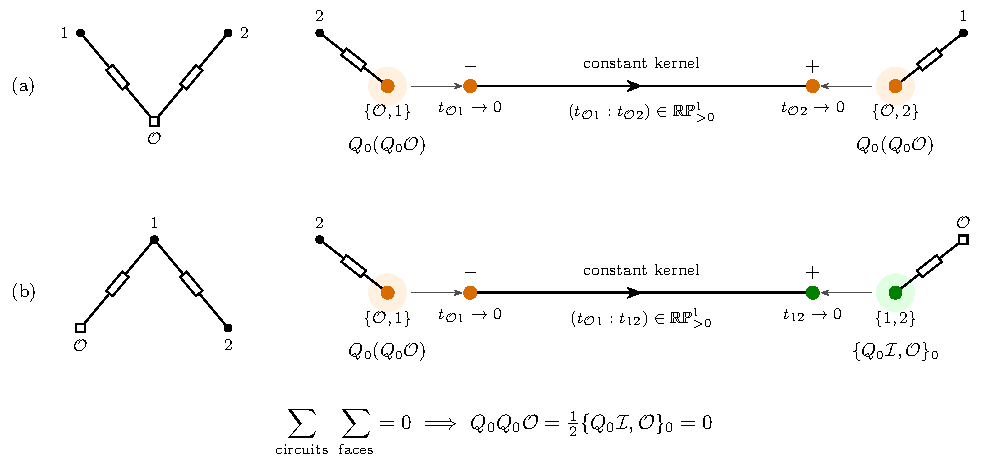
\includegraphics[width=.98\linewidth]{figures/circuits/nilpotence_Q0Q0.pdf}
\caption{$Q_0^2=0$ in $\mathcal N=4$ Yang--Mills theory, from the ends of integration domains. Each circuit joins $\mathcal O$ and two interaction nodes by two resistors; its integration domain is the interval $\mathbb{RP}^1_{>0}$ of the two resistances, and the ends of the interval are the two shorts. Orange: the island contains $\mathcal O$, and the face is the composite $Q_0(Q_0\mathcal O)$. Green: the island holds interactions only, and the face is $\{Q_0\mathcal I,\mathcal O\}_0$. The tree currents do not depend on the resistances, so the kernel is constant along the interval and the two ends enter with opposite orientations. (a) $\mathcal O$ in the middle: both ends are composites. (b) $\mathcal O$ at an end: the composite pairs with $\{Q_0\mathcal I,\mathcal O\}_0$, which vanishes since $Q_0\mathcal I=0$ (Theorem~\ref{thm:interaction-consistency}).}
\label{fig:nilpotence-Q0Q0}
\end{figure}
\begin{figure}[H]
\centering
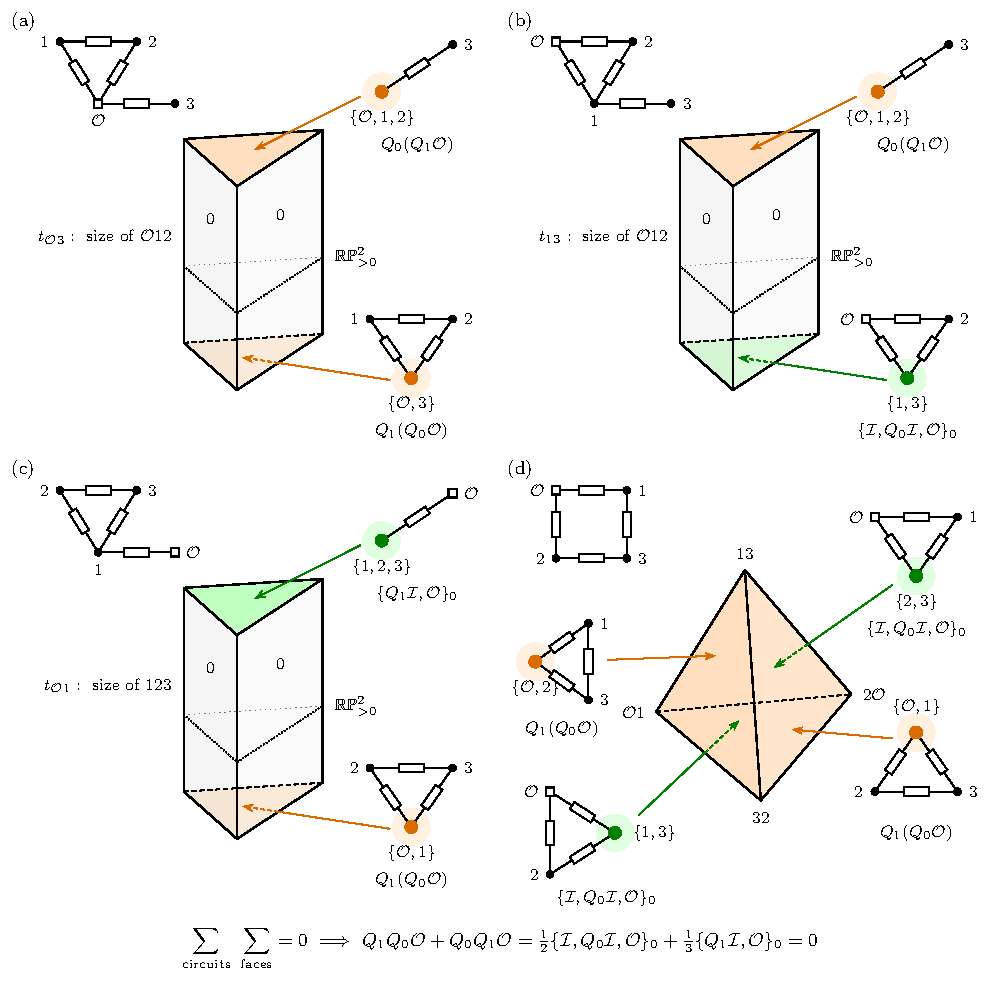
\includegraphics[width=.98\linewidth,height=.8\textheight,keepaspectratio]{figures/circuits/nilpotence_Q0Q1.pdf}
\caption{$Q_0Q_1+Q_1Q_0=0$: the four $\mathcal N=4$ circuits with $\mathcal O$, three interaction nodes and four resistors, and their three-dimensional integration domains. (a)--(c) A triangle and a tail share a node. The domain is the prism of the ratio between the tail and the triangle over the ratios of the triangle, $\mathbb{RP}^2_{>0}$: the bottom is the shorted tail, the top the shorted triangle. On a side one triangle resistor is shorted, the outer network has parallel resistors, and the current form, which depends only on the ratios of the triangle, vanishes. (d) The square: the domain is the tetrahedron of the four resistances, and each facet is the short of one resistor. Colours as in Figure~\ref{fig:nilpotence-Q0Q0}; the green faces vanish since $Q_0\mathcal I=Q_1\mathcal I=0$.}
\label{fig:nilpotence-Q0Q1}
\end{figure}
\begin{figure}[H]
\centering
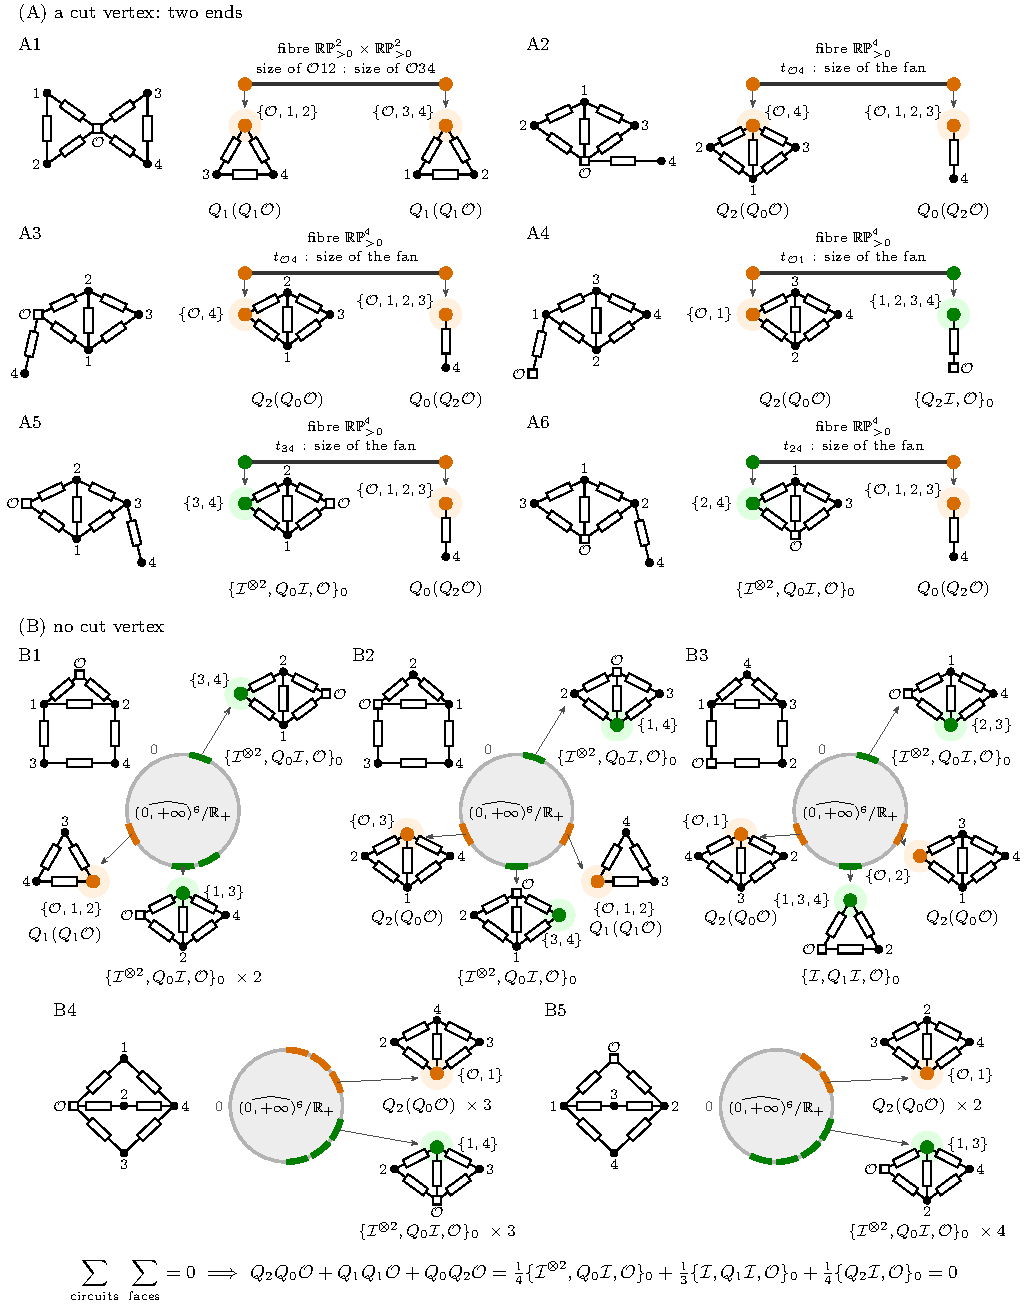
\includegraphics[width=.98\linewidth,height=.86\textheight,keepaspectratio]{figures/circuits/nilpotence_Q1Q1.pdf}
\caption{$Q_1^2+Q_0Q_2+Q_2Q_0=0$: the eleven $\mathcal N=4$ circuits with $\mathcal O$, four interaction nodes and six resistors; their integration domains are five-dimensional. (A) One node splits the circuit into two Laman blocks, two triangles or a two-loop fan and a tail. The current form depends only on the ratios inside each block, so only the two ends of the ratio between the blocks contribute. (B) Circuits without such a node, with the domain drawn schematically: the coloured arcs are the contributing faces, and the other faces carry zero. Colours as in Figure~\ref{fig:nilpotence-Q0Q0}; the green faces vanish since $Q_0\mathcal I=Q_1\mathcal I=Q_2\mathcal I=0$.}
\label{fig:nilpotence-Q1Q1}
\end{figure}


\begin{theorem}\label{thm:interaction-consistency}
Suppose that $\bar W$ is gauge invariant and the matter representation obeys
\begin{equation}\label{eq:2.41}
\operatorname{Tr}_R\!\left(t_A\{t_B,t_C\}\right)=0.
\end{equation}
For the interaction \eqref{eq:B.10}, the integrated interaction satisfies
\begin{equation}
\bar\partial\mathcal I=0,\qquad
Q_0\mathcal I=0,\qquad Q_1\mathcal I=0,\qquad
Q_2\mathcal I=Q_3\mathcal I=\cdots=0.
\end{equation}
Consequently, $\mathcal I$ satisfies \eqref{eq:2.40}, $\bigl(\bar\partial+Q_0+\sum_{n\ge1}\hbar^nQ_n\bigr)\mathcal I=0$, and $\mathbf Q^2=0$ by Lemma~\ref{lem:qme-nilpotence}.
\end{theorem}

\begin{proof}
The free differential $\bar\partial$ maps the integrated Dolbeault density of $\mathcal I$ to a total derivative. The gauge and matter vertices satisfy the classical master equation by
\begin{equation*}
C^A{}_{B[C}C^B{}_{DE]}=0,
\qquad [t_A,t_B]=iC^C{}_{AB}t_C.
\end{equation*} Since $\bar W$ contains no $\mathsf b$ or $\beta$, its self-bracket vanishes, and, up to holomorphic total derivatives,
\begin{equation*}
\begin{aligned}
Q_0\mathcal I=\{\mathcal I,\mathcal I\}_0
={}&-2ig\mathsf c^A(t_A)^j{}_i\gamma_j
\frac{\partial\bar W}{\partial\gamma_i}\\
&-2g\mathsf c^AC^B{}_{AC}\mathsf w^C_{\dot a}
\frac{\partial_L\bar W}{\partial\mathsf w^B_{\dot a}}=0.
\end{aligned}
\end{equation*}
The last equality is gauge invariance of $\bar W$.

The circuit of $Q_1\mathcal I$ is a triangle of three gauge or matter nodes, whose loop carries a trace. The two orientations of the matter triangle give
$-ig^3\operatorname{Tr}_R(t_A\{t_B,t_C\})\mathsf c_1^A\mathsf c_2^B\mathsf c_3^C$.
The gauge triangle has the symmetric adjoint trace, which vanishes. The triangle kernel~\eqref{eq:1.25}, the prefactor in~\eqref{eq:2.3}, and $\lambda_{v,+\dot a}=-\tfrac12\partial_{v,+\dot a}$ give
\begin{equation*}
-\frac{1}{2!\,8\pi^2}\cdot\frac12\cdot\frac14\cdot(-ig^3)
=\frac{ig^3}{128\pi^2}.
\end{equation*}
Hence
\begin{equation}
Q_1\mathcal I
=\frac{ig^3}{128\pi^2}
\operatorname{Tr}_R\!\left(t_A\{t_B,t_C\}\right)
\mathsf c^A(\partial_{+\dot a}\mathsf c^B)
(\partial_+{}^{\dot a}\mathsf c^C)=0.
\end{equation}

A circuit of $Q_n\mathcal I$ has $n+2$ interaction nodes and $2n+1$ resistors, and each resistor takes its own antifield terminal (Lemma~\ref{lem:antifield}): a gauge or matter node has one, a superpotential node none. Thus
\begin{equation*}
2n+1\le n+2-\#(\bar W\text{ nodes}),
\end{equation*}
which is impossible for $n\ge2$. Finally,
$Q_n\mathcal I=\{\mathcal I^{\otimes(n+2)}\}_0/(n+1)!$
gives~\eqref{eq:2.40}.
\end{proof}


\section{Quantum multiplication and the Leibniz rule}
\label{sec:product}

The differential $Q_1$ contains two input derivatives. Acting on $AB$, these derivatives can land on different factors, producing a cross-contraction. For homogeneous operators $A,B$, with $|A|$ the fermion number of $A$, the zero-input-jet part of the $\mathcal N=4$ operator gives
\begin{equation}\label{eq:2.29}
\begin{aligned}
&Q_1(AB)-(Q_1A)B-(-1)^{|A|}A(Q_1B)\\
&\qquad=-\frac1{64\pi^2}\int d^3\theta\,
C_{XRD}C_{YRE}
(\partial_{+\dot a}C^D)(\partial_+{}^{\dot a}C^E)
\frac{\delta A}{\delta C^X}\frac{\delta B}{\delta C^Y}.
\end{aligned}
\end{equation}
Even when both $A$ and $B$ are annihilated by $Q_0$ and $Q_1$, this cross-contraction can be nonzero. Their ordinary product then fails to be closed at one loop. The higher corrections $Q_n$ likewise act on several input fields and produce contractions shared between the two factors, violating the ordinary Leibniz rule. This raises an apparent tension with the ring structure of supercharge cohomology: supersymmetry acts as a graded derivation on separated operator products, and the product of two closed operators should again define a closed class.

The issue arises when the insertions are brought together and expressed in the renormalized local-field coordinates. The quantum multiplication is the marked product of \cite[Sections 4.3 and 4.5]{higher} at every perturbative order; \cite[footnote 28]{semichiral} states that $\mathbf Q$ obeys the Leibniz rule for the quantum normal-ordering product, which Theorem~\ref{thm:normal-ordering} identifies with the marked product in cohomology. The quadratic identities of the higher brackets, together with nilpotence of the quantum BV differential, give the corrected Leibniz identity \eqref{eq:chain}. Thus $\mathbf QA=\mathbf QB=0$ implies $\mathbf Q(A\star B)=0$. We first prove this identity and, from the marked quadratic identities with three insertions, the ring laws on cohomology, then give the graph formula and evaluate the one- and two-loop corrections. Section~\ref{sec:normal-ordering} proves the identification with quantum normal ordering and evaluates an explicit associator.

For the enumeration of $\mathbf Q$-cohomology representatives, the quantum product need not be computed. It is an explicit construction showing that the product of two quantum cocycles is a quantum cocycle: for quantum cocycles $A$ and $B$, $A\star B$ is a quantum cocycle completing $A_0B_0$, and it is lifted exactly when it becomes a quantum coboundary. In the successive homotopy transfer of Section~\ref{sec:homotopy-transfer}, which is the algorithm of the lifting tests, it induces the ordinary product of leading representatives on every page (Theorem~\ref{thm:quantum-bps-ring}); Section~\ref{sec:order-by-order} gives its first orders.

\subsection{The Leibniz rule of the quantum supercharge}
\label{sec:dressed-chain}

Here $\{\cdot\}_0$ denotes the brackets of Section~\ref{sec:setup}, at vanishing spectral parameter. The quantum differential and the interacting bracket of two operators are
\begin{equation}\label{eq:2.51}
\mathbf Q\mathcal O=\sum_{s\ge1}\frac{\hbar^{s-1}}{s!}\{\mathcal I^{\otimes s},\mathcal O\}_0,\qquad
\{X,Y\}_{\mathcal I}=\sum_{r\ge0}\frac{\hbar^r}{r!}\{\mathcal I^{\otimes r},X,Y\}_0 .
\end{equation}

\begin{theorem}[Leibniz rule]\label{thm:leibniz}
Suppose that the interaction satisfies \eqref{eq:2.40}. For homogeneous operators $X,Y$, with $|X|$ the fermion number of $X$,
\begin{equation}\label{eq:2.52}
\mathbf Q\{X,Y\}_{\mathcal I}
-\{\mathbf QX,Y\}_{\mathcal I}
+(-1)^{|X|}\{X,\mathbf QY\}_{\mathcal I}=0,
\end{equation}
and the quantum product obeys
\begin{equation}\label{eq:chain}
\mathbf Q(A\star B)
=(\mathbf QA)\star B+(-1)^{|A|}A\star(\mathbf QB).
\end{equation}
In particular, quantum multiplication takes quantum cocycles to quantum cocycles and descends to $\mathbf Q$-cohomology.
\end{theorem}

\begin{proof}
For $N\ge1$ interaction entries and the entries $X,Y$, the quadratic identity of the higher brackets \cite[Section 3.2]{operatope}, \cite[Theorem 7]{Wang}, \cite[Equation (4.19)]{higher}, in the conventions of \eqref{eq:2.46}, sorts its terms by the content of the inner bracket:
\begin{equation}\label{eq:quadratic-two}
\begin{aligned}
0={}&\underbrace{\sum_{r=0}^{N-1}\binom Nr\{\mathcal I^{\otimes(N-r)},\{\mathcal I^{\otimes r},X,Y\}_0\}_0}_{\text{inner bracket contains }X\text{ and }Y}
-\underbrace{\sum_{r=1}^{N}\binom Nr\{\mathcal I^{\otimes(N-r)},\{\mathcal I^{\otimes r},X\}_0,Y\}_0}_{\text{inner bracket contains }X}\\
&+(-1)^{|X|}\underbrace{\sum_{r=1}^{N}\binom Nr\{\mathcal I^{\otimes(N-r)},X,\{\mathcal I^{\otimes r},Y\}_0\}_0}_{\text{inner bracket contains }Y}
+\underbrace{\sum_{k=2}^{N}\binom Nk\{\mathcal I^{\otimes(N-k)},\{\mathcal I^{\otimes k}\}_0,X,Y\}_0}_{\text{inner bracket contains only interactions}}.
\end{aligned}
\end{equation}
Multiply by $\hbar^{N-1}/N!$ and sum over $N\ge1$. Since $\binom Nr/N!=1/(r!\,(N-r)!)$, each double sum factorizes into an outer series in $s=N-r$ and an inner series:
\begin{equation}\label{eq:quadratic-two-summed}
\begin{aligned}
0={}&\underbrace{\sum_{s\ge1}\frac{\hbar^{s-1}}{s!}\Big\{\mathcal I^{\otimes s},\sum_{r\ge0}\frac{\hbar^r}{r!}\{\mathcal I^{\otimes r},X,Y\}_0\Big\}_0}_{\mathbf Q\{X,Y\}_{\mathcal I}}
-\underbrace{\sum_{s\ge0}\frac{\hbar^{s}}{s!}\Big\{\mathcal I^{\otimes s},\sum_{r\ge1}\frac{\hbar^{r-1}}{r!}\{\mathcal I^{\otimes r},X\}_0,Y\Big\}_0}_{\{\mathbf QX,Y\}_{\mathcal I}}\\
&+(-1)^{|X|}\underbrace{\sum_{s\ge0}\frac{\hbar^{s}}{s!}\Big\{\mathcal I^{\otimes s},X,\sum_{r\ge1}\frac{\hbar^{r-1}}{r!}\{\mathcal I^{\otimes r},Y\}_0\Big\}_0}_{\{X,\mathbf QY\}_{\mathcal I}}\\
&+\underbrace{\sum_{s\ge0}\frac{\hbar^{s+1}}{s!}\Big\{\mathcal I^{\otimes s},\sum_{k\ge2}\frac{\hbar^{k-2}}{k!}\{\mathcal I^{\otimes k}\}_0,X,Y\Big\}_0}_{0\text{ by \eqref{eq:2.40}}}.
\end{aligned}
\end{equation}
The inner series are \eqref{eq:2.51} and the left side of \eqref{eq:2.40}; this is \eqref{eq:2.52}. The Jacobi identity expresses the Leibniz rule for an adjoint action on a bracket, and \eqref{eq:2.52} is its higher $L_\infty$ form, with the interaction insertions supplying every perturbative order \cite[Sections 4.3--4.5]{higher}.

For the decoupled auxiliary pair of Section~\ref{sec:dressed-definition}, $|a|=0$, $|b_{\mathrm{aux}}|=1$, and both holomorphic auxiliary letters are $\mathbf Q$-closed. Thus
\begin{equation*}
\mathbf Q(Aa)=(\mathbf QA)a,
\qquad
\mathbf Q(b_{\mathrm{aux}}B)=-b_{\mathrm{aux}}\mathbf QB.
\end{equation*}
The unique auxiliary contraction gives
\begin{equation*}
\left.\{Aa,b_{\mathrm{aux}}B\}_{\mathcal I}
\right|_{\mathrm{aux}=0}
=\sum_{n\ge0}\frac{\hbar^n}{n!}
\{\mathcal I^{\otimes n},A,B\}^{\gamma,0}
=A\star B.
\end{equation*}
Set $X=Aa$ and $Y=b_{\mathrm{aux}}B$ in \eqref{eq:2.52}, and extract this contraction:
\begin{equation*}
0=\mathbf Q(A\star B)
-(\mathbf QA)\star B-(-1)^{|A|}A\star(\mathbf QB).
\end{equation*}
Consequently, $\mathbf QA=\mathbf QB=0$ gives $\mathbf Q(A\star B)=0$. For homogeneous $X,Y$ with $|X|=|A|+1$ and $|Y|=|B|+1$, the same identity and $\mathbf Q^2=0$ (Lemma~\ref{lem:qme-nilpotence}) give
\begin{equation}\label{eq:representatives}
\begin{aligned}
&(A+\mathbf QX)\star(B+\mathbf QY)-A\star B\\
&\qquad=\mathbf Q\bigl(X\star B+(-1)^{|A|}A\star Y
+X\star\mathbf QY\bigr).
\end{aligned}
\end{equation}
The resulting cohomology class is therefore independent of representatives.
\end{proof}
Equation~\eqref{eq:2.52} collects the shorts of Appendix~\ref{sec:B-short-circuits}: its three terms are the islands containing both $X$ and $Y$, only $X$, and only $Y$, and the islands of interactions alone cancel by \eqref{eq:2.40}. Appendix~\ref{sec:B-leibniz} reads \eqref{eq:chain} directly off the marked circuits.


\subsection{The quantum BPS ring}
\label{sec:ring}

Write $[\cdot]_{\mathbf Q}$ for the class of a quantum cocycle.

\begin{theorem}\label{thm:quantum-bps-ring}
Suppose the marked higher operations satisfy their quadratic identities
and the interaction satisfies \eqref{eq:2.40}. The quantum product
\eqref{eq:star} induces an associative, graded-commutative, unital
multiplication on $H(\mathbf Q)$. For homogeneous quantum cocycles
$A,B,D$,
\begin{equation}\label{eq:ring-associativity}
[(A\star B)\star D]_{\mathbf Q}
=[A\star(B\star D)]_{\mathbf Q},
\end{equation}
\begin{equation}\label{eq:ring-commutativity}
[A\star B]_{\mathbf Q}
=(-1)^{|A||B|}[B\star A]_{\mathbf Q}.
\end{equation}
The unit is strict:
\begin{equation}\label{eq:ring-unit}
A\star1=1\star A=A.
\end{equation}
In the successive homotopy transfer of Section~\ref{sec:homotopy-transfer}, the quantum product induces on every page $E_r$ the ordinary product of leading representatives, and every $d_r$ is a derivation of it.
\end{theorem}
\begin{proof}
The chain identity \eqref{eq:chain} makes the product well-defined
on cohomology. A class of $E_r$ has a representative $a+\hbar a_1+\cdots$ whose $\mathbf Q$-variation starts at order $\hbar^r$ with $d_ra$. Since $A\star B=AB+O(\hbar)$, the product of two such representatives has leading term $ab$, and by \eqref{eq:chain} its $\mathbf Q$-variation starts at order $\hbar^r$ with $(d_ra)b+(-1)^{|a|}a\,d_rb$; on $E_1$ this is the first line of \eqref{eq:2.55}. For the unit, the identity insertion has no fields, so in a marked circuit with $n\ge1$ interaction nodes it is wired only by the marked resistor. It is a dead end: the marked resistor carries the current injected at the identity insertion whatever its resistance, so this resistance moves no current and the current form vanishes. Only the zero-interaction marked segment contributes.

For three closed insertions $X,Y,Z$, sum the quadratic identities
with all interaction entries, as in \cite[Sections 4.3 and 4.5]{higher}.
Distributing $n$ interactions between two brackets gives
$\binom{n}{j}/n!=1/(j!(n-j)!)$.
The pure-interaction terms vanish by \eqref{eq:2.40}, and the
single-input terms vanish by closure. With the ordered-bracket sign
of \eqref{eq:A.28}, the remaining identity is
\begin{equation}\label{eq:ring-twisted-jacobi}
\begin{aligned}
0={}&\{X,\{Y,Z\}_{\mathcal I}\}_{\mathcal I}
-\{\{X,Y\}_{\mathcal I},Z\}_{\mathcal I}\\
&-(-1)^{(|X|+1)(|Y|+1)}
\{Y,\{X,Z\}_{\mathcal I}\}_{\mathcal I}\\
&+\mathbf Q\sum_{n\ge0}\frac{\hbar^{n+1}}{n!}
\{\mathcal I^{\otimes n},X,Y,Z\}_0.
\end{aligned}
\end{equation}
The sign in \eqref{eq:A.28} is $(-1)^{|X|}$ for two inputs
and $(-1)^{|Y|}$ for three; the even interaction entries do not
change these factors. A ternary graph with $n$ interactions has
$n+3$ vertices and $2n+3$ edges, hence loop number $n+1$.
This fixes the power of $\hbar$ in the last line.

Take two independent copies $(a_1,b_{\mathrm{aux},1})$ and
$(a_2,b_{\mathrm{aux},2})$ of the free auxiliary pair in
Section~\ref{sec:dressed-definition}. Each $a_i$ is even and
each $b_{\mathrm{aux},i}$ is odd. Substitute
\[
X=Aa_1,\qquad Y=Da_2,\qquad
Z=b_{\mathrm{aux},1}b_{\mathrm{aux},2}B.
\]
The last insertion is the root. Set the two auxiliary displacements
to zero and contract each auxiliary pair once. This marks the edges
$AB$ and $DB$, as in Figure~\ref{fig:common-root-marks}.

\par\medskip
\noindent\begin{minipage}{\linewidth}
\begingroup
\captionsetup{hypcap=false}
\centering
\tikzset{
  commonroot vertex/.style={circle,draw=black,fill=white,inner sep=1.6pt},
  commonroot root/.style={circle,draw=black,double,fill=white,inner sep=1.7pt},
  commonroot first/.style={red!75!black,line width=.85pt,-{Latex[length=1.7mm]}},
  commonroot second/.style={blue!75!black,line width=.85pt,-{Latex[length=1.7mm]}}
}
\begin{minipage}[t]{.48\linewidth}
\centering
\begin{tikzpicture}[font=\small]
  \path[use as bounding box] (-.15,-.35) rectangle (6.0,3.1);
  \node at (2.9,2.85) {(a) Both marks end at the root};
  \node[commonroot vertex,label=above:{$Aa_1$}] (A) at (.8,2.05) {};
  \node[commonroot vertex,label=above:{$Da_2$}] (D) at (5.0,2.05) {};
  \node[commonroot root] (B) at (2.9,.70) {};
  \draw[commonroot first] (A) -- (B);
  \draw[commonroot second] (D) -- (B);
  \node[below=4pt] at (B) {$b_{\mathrm{aux},1}b_{\mathrm{aux},2}B$};
\end{tikzpicture}
\end{minipage}\hfill
\begin{minipage}[t]{.48\linewidth}
\centering
\begin{tikzpicture}[font=\small]
  \path[use as bounding box] (-.15,-.35) rectangle (6.0,3.1);
  \node at (2.9,2.85) {(b) Collapse $A,B$ at $B$};
  \node[commonroot vertex,label=above:{$Da_2$}] (D) at (.85,1.8) {};
  \node[commonroot root] (AB) at (4.2,1.0) {};
  \draw[commonroot second] (D) -- (AB);
  \node[below=5pt,align=center] at (AB)
    {$b_{\mathrm{aux},2}(A\star B)$};
  \node[font=\footnotesize] at (2.85,-.12)
    {The second auxiliary field stays at the root.};
\end{tikzpicture}
\end{minipage}
\par\smallskip
\begin{minipage}[t]{.48\linewidth}
\centering
\begin{tikzpicture}[font=\small]
  \path[use as bounding box] (-.15,-.35) rectangle (6.0,3.1);
  \node at (2.9,2.85) {(c) Collapse $D,B$ at $B$};
  \node[commonroot vertex,label=above:{$Aa_1$}] (A) at (.85,1.8) {};
  \node[commonroot root] (DB) at (4.2,1.0) {};
  \draw[commonroot first] (A) -- (DB);
  \node[below=5pt,align=center] at (DB)
    {$b_{\mathrm{aux},1}(D\star B)$};
  \node[font=\footnotesize] at (2.85,-.12)
    {The first auxiliary field stays at the root.};
\end{tikzpicture}
\end{minipage}\hfill
\begin{minipage}[t]{.48\linewidth}
\centering
\begin{tikzpicture}[font=\small]
  \path[use as bounding box] (-.15,-.35) rectangle (6.0,3.1);
  \node at (2.9,2.85) {(d) Collapse $A,D$};
  \node[commonroot vertex] (AD) at (1.0,1.45) {};
  \node[above=9pt,align=center] at (AD)
    {$\{Aa_1,Da_2\}_{\mathcal I}$};
  \node[commonroot root] (B) at (4.4,1.45) {};
  \node[above=9pt,align=center] at (B)
    {$b_{\mathrm{aux},1}b_{\mathrm{aux},2}B$};
  \draw[commonroot first] (AD) to[bend left=17] (B);
  \draw[commonroot second] (AD) to[bend right=17] (B);
  \node at (2.8,.55) {$P\wedge P=0,\qquad K\wedge P=0$};
  \node[font=\footnotesize] at (2.85,-.12)
    {Both marks now join the same two vertices.};
\end{tikzpicture}
\end{minipage}
\captionof{figure}{The common-root contraction and its three pair-collapse
channels. Red and blue arrows mark the first and second auxiliary
pairs; double circles mark the root. Only auxiliary contractions are
shown. Each component may also contain interaction vertices and physical
contractions. The labels in (b) and (c) display the surviving fields;
their Koszul signs are given in the proof.}
\label{fig:common-root-marks}
\endgroup
\end{minipage}
\par\medskip

For a collapse containing $A,B$, the second auxiliary field stays at
$B$; for a collapse containing $D,B$, the first stays there. The root
coordinate is fixed to zero in \eqref{eq:A.28}, so output Taylor
derivatives act on the nonroot surviving fields. The auxiliary
spectator at $B$ therefore remains undifferentiated, including when
the physical inputs contain arbitrary holomorphic derivatives.
The left derivatives and the ordered-bracket sign give
\begin{equation}\label{eq:ring-root-contractions}
\begin{aligned}
\left.\{Aa_1,b_{\mathrm{aux},1}b_{\mathrm{aux},2}B\}_{\mathcal I}
\right|_{a_1=b_{\mathrm{aux},1}=0}
&=(-1)^{|A|}b_{\mathrm{aux},2}(A\star B),\\
\left.\{Da_2,b_{\mathrm{aux},1}b_{\mathrm{aux},2}B\}_{\mathcal I}
\right|_{a_2=b_{\mathrm{aux},2}=0}
&=(-1)^{|D|+1}b_{\mathrm{aux},1}(D\star B).
\end{aligned}
\end{equation}
The restrictions set the indicated pair to zero after contraction.
In the second line the odd derivative passes through
$b_{\mathrm{aux},1}$, contributing the extra minus sign.

The third binary channel first collapses $A,D$. Both marked resistors
then join that collapsed node to $B$: they are in parallel, and their
proportional currents kill the measure for every holomorphic derivative
(Theorem~\ref{thm:no-parallel}, \eqref{eq:1.13}). Consequently,
\begin{equation}\label{eq:ring-parallel-channel}
\left.
\{\{Aa_1,Da_2\}_{\mathcal I},
b_{\mathrm{aux},1}b_{\mathrm{aux},2}B\}_{\mathcal I}
\right|_{\mathrm{aux}=0}=0.
\end{equation}
Substituting \eqref{eq:ring-root-contractions} and
\eqref{eq:ring-parallel-channel} into
\eqref{eq:ring-twisted-jacobi}, each of its three nested brackets becomes a product of three operators:
\begin{equation}\label{eq:ring-twisted-jacobi-substituted}
0=\underbrace{(-1)^{|D|+1}A\star(D\star B)}_{\{X,\{Y,Z\}_{\mathcal I}\}_{\mathcal I}}
-\underbrace{0}_{\substack{\{\{X,Y\}_{\mathcal I},Z\}_{\mathcal I}:\\\text{parallel marks}}}
\underbrace{-(-1)^{(|A|+1)(|D|+1)+|A|}D\star(A\star B)}_{-(-1)^{(|X|+1)(|Y|+1)}\{Y,\{X,Z\}_{\mathcal I}\}_{\mathcal I}}
+\underbrace{\mathbf Q\,H}_{\mathbf Q\text{-exact}},
\end{equation}
with $H$ the bracket in the last line of \eqref{eq:ring-twisted-jacobi} at these inputs. The middle term vanishes, so only the two bracketings $A\star(D\star B)$ and $D\star(A\star B)$ remain. Multiplying by $(-1)^{|D|+1}$ gives the local homotopy
\begin{equation}\label{eq:ring-common-root-homotopy}
\begin{aligned}
&A\star(D\star B)-(-1)^{|A||D|}D\star(A\star B)\\
&\quad=(-1)^{|D|}\mathbf Q
\left[
\left.\sum_{n\ge0}\frac{\hbar^{n+1}}{n!}
\{\mathcal I^{\otimes n},Aa_1,Da_2,
 b_{\mathrm{aux},1}b_{\mathrm{aux},2}B\}_0
\right|_{\mathrm{aux}=0}\right].
\end{aligned}
\end{equation}
Its $n$-interaction term has $2n+1$ physical contractions.
The interactions supply at most $n$ fields of type $\mathsf b$ or
$\beta$, so at least $n+1$ must come from the inputs. The homotopy
is therefore a finite sum of local operators for finite polynomial
inputs.

Setting $B=1$ proves graded commutativity. For three closed inputs,
\eqref{eq:chain}, graded commutativity, and
\eqref{eq:ring-common-root-homotopy} give
\begin{equation}\label{eq:ring-associativity-proof}
\begin{aligned}
[(A\star B)\star D]_{\mathbf Q}
&\underset{\eqref{eq:ring-commutativity}}{=}(-1)^{(|A|+|B|)|D|}[D\star(A\star B)]_{\mathbf Q}\\
&\underset{\eqref{eq:ring-common-root-homotopy}}{=}(-1)^{|B||D|}[A\star(D\star B)]_{\mathbf Q}\\
&\underset{\eqref{eq:ring-commutativity}}{=}[A\star(B\star D)]_{\mathbf Q}.
\end{aligned}
\end{equation}
The $\mathbf Q$-exact term of \eqref{eq:ring-common-root-homotopy} drops out of the classes; this is the potential $\mathbf Q$-exact difference between the two bracketings in \eqref{eq:ring-associativity}.
This proves the stated ring laws.
\end{proof}

\subsection{The graph formula}

The quantum product of Section~\ref{sec:dressed-definition} corrects the cross-contraction \eqref{eq:2.29}. For a physical edge $(v,w)$, the operator $\Delta_{vw}$ contracts one field at vertex $v$ with its BV conjugate at vertex $w$, using the pairing~\eqref{eq:A.20}. In the $\mathcal N=4$ superfield variables, at fixed vertex positions,
\begin{equation*}
\Delta_{vw}=-\delta^{DE}\int d^3\theta\,
\frac{\delta}{\delta C_v^D(\theta)}
\frac{\delta}{\delta C_w^E(\theta)}.
\end{equation*}
Here $C_v^D$ is the field at vertex $v$, and the fibre derivatives are given by~\eqref{eq:A.16}. Composing these contractions in edge order gives the graph coefficient

\begin{equation}\label{eq:2.31}
\begin{aligned}
\frac1{n!}\{\mathcal I^{\otimes n},A,B\}^{\gamma,0}
={}&\frac{(-1)^n}{n!(8\pi^2)^n}
\sum_{\substack{\Gamma\ \mathrm{labelled,\ Laman}\\
|\Gamma_0|=n+2,\ |\Gamma_1|=2n+1\\(n+1,n+2)\in\Gamma_1}}
\Bigg[\mathcal I_\Gamma^{\mathrm{raw\ cut}}(\lambda;z)\\
&\qquad\times\prod_{(v,w)\in\Gamma_1\setminus\{(n+1,n+2)\}}^{\mathrm{edge\ order}}
\Delta_{vw}(\mathcal I_1\cdots\mathcal I_nA_{n+1}B_{n+2})\Bigg]_{\mathrm{jets},\,x=z=0}.
\end{aligned}
\end{equation}

The marked edge $(n+1,n+2)$ contributes its kernel; the ordered product contains the physical contractions. In the subscript $\mathrm{jets}$, each derivative on a contracted input field differentiates the kernel through its edge displacement, while $\lambda_v$ differentiates the surviving fields at vertex $v$. The positions and displacements are then set to zero. The graph restrictions of Section~\ref{sec:forests} reduce this sum to product forests.

\Needspace{19\baselineskip}
\subsection{One and two loops in \texorpdfstring{$\mathcal N=4$}{N=4} Yang--Mills theory}
\label{sec:product-loops}

The one-loop triangle has vertices $1:\mathcal I$, $2:A$ and $3:B$, and marked edge $\gamma=\{(2,3)\}$. Pairing its displacement exponential with the spatial functional derivatives of \eqref{eq:2.10} gives
\begin{equation}\label{eq:2.34}
\begin{aligned}
\{\mathcal I,A,B\}^{\{(2,3)\},0}
={}&\frac{i}{32\pi^2}\int_0^1dr_1\int_0^{1-r_1}dr_2
\int d^3\theta\,C_{XYZ}\\
&\times\int d^4z_1\,d^4z_2\\
&\times(\partial_{+\dot a}C^X)
\big(r_1z_1+(1-r_1)z_2,\theta\big)\\
&\times\left.
\partial_{2,+}{}^{\dot a}
\left(\frac{\delta A(x_2)}{\delta C^Y(x_2+z_1,\theta)}\right)
\right|_{x_2=r_2(z_2-z_1)}
\frac{\delta B(0)}{\delta C^Z(z_2,\theta)}.
\end{aligned}
\end{equation}
The functional derivative of $A(x_2)$ is taken at $x_2+z_1$; $\partial_{2,+}{}^{\dot a}$ differentiates its surviving fields at fixed $z_1$ before the displayed positions are substituted.

At zero input-jet order, the triangle moment $1/2$ gives the leading correction, whose graph is drawn in \cite[Figure 7, middle]{higher},

\begin{equation}\label{eq:2.35}
\{\mathcal I,A,B\}^{\gamma,0}=\frac{i}{64\pi^2}\int d^3\theta\,C_{XYZ}(\partial_{+\dot a}C^X)\,\partial_+{}^{\dot a}\Big(\frac{\delta A}{\delta C^Y}\Big)\frac{\delta B}{\delta C^Z}.
\end{equation}

At two loops the physical graphs have four edges. They consist of a book and two triangles attached to opposite inputs (Figure~\ref{fig:two-loop-product}). Their ordered edges, for $3=A$ and $4=B$, are
\begin{equation}\label{eq:productedges}
\begin{aligned}
\Gamma_{\mathrm{book}}&:(13,14,23,24,34),\\
\Gamma_A&:(12,13,23,24,34),\\
\Gamma_B&:(12,14,23,24,34).
\end{aligned}
\end{equation}
\begin{figure}[H]
\centering
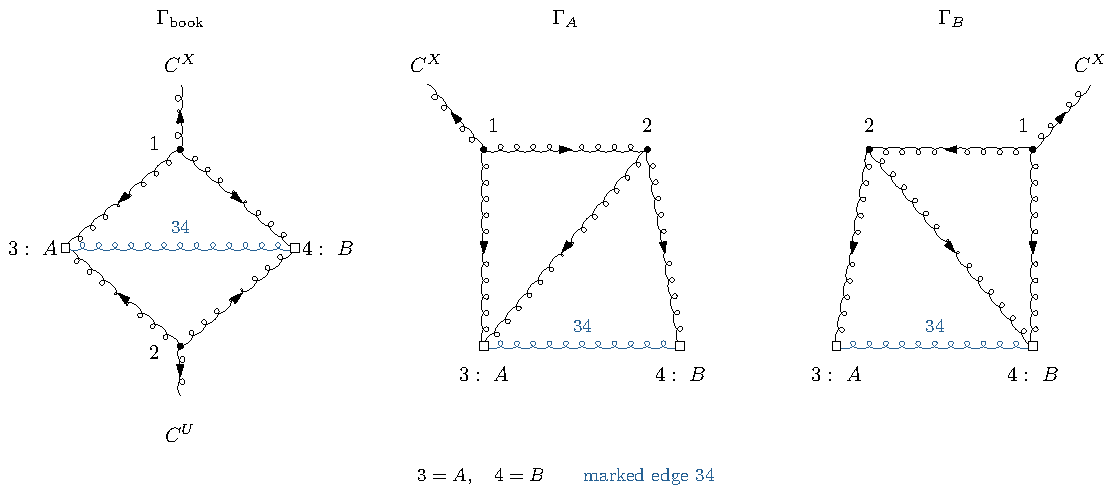
\includegraphics[width=0.99\linewidth,height=.70\textheight,keepaspectratio]{figures/two_loop_product_feynarts.pdf}
\caption{The two-loop quantum-product graphs $\Gamma_{\mathrm{book}}$, $\Gamma_A$ and $\Gamma_B$. Squares are the insertions $3:A$ and $4:B$; dots are cubic interactions. Black arrows orient the physical contractions, and the blue edge $(3,4)$ carries the auxiliary pairing. The book leaves $C^X,C^U$ uncontracted; each triangle leaves $C^X$.}
\label{fig:two-loop-product}
\end{figure}

The last edge is marked. The kernels at zero displacement are
\begin{equation}\label{eq:productkernels}
\begin{aligned}
\mathcal I_{\Gamma_{\mathrm{book}}}^{\mathrm{raw\ cut}}(\lambda;0)
&=\frac1{24}
\big[\lambda_{1,+\dot a}(\lambda_{2,+}{}^{\dot a}+2\lambda_{3,+}{}^{\dot a})\big]
\big[\lambda_{2,+\dot b}(\lambda_{1,+}{}^{\dot b}+2\lambda_{3,+}{}^{\dot b})\big],\\
\mathcal I_{\Gamma_A}^{\mathrm{raw\ cut}}(\lambda;0)
&=-\frac1{24}(\lambda_{1,+\dot a}\lambda_{3,+}{}^{\dot a})^2,\\
\mathcal I_{\Gamma_B}^{\mathrm{raw\ cut}}(\lambda;0)
&=\frac1{24}(\lambda_{1,+\dot a}\lambda_{3,+}{}^{\dot a})^2.
\end{aligned}
\end{equation}
\Needspace{6\baselineskip}
Including the interaction factor $1/2!$ and the vertex labellings gives Wick coefficients $\tfrac12C_{XYZ}C_{UVW}$, $-C_{XYR}C_{RZW}$, and $-C_{XZR}C_{RYW}$.

The functional derivatives \eqref{eq:2.10} are taken at the displayed insertion shifted by the relative displacement, as in $\delta/\delta C^Y(x_3+z,\theta)$. Each $\partial_v$ differentiates the surviving fields at vertex $v$ at fixed displacements, before the translated positions are substituted. The edge between interaction vertices has zero displacement; the $z$-integrals run over the physical edges ending at an insertion.

\begin{equation}\label{eq:product2book}
\begin{aligned}
&\left.\frac12\{\mathcal I,\mathcal I,A,B\}^{\gamma,0}\right|_{\Gamma_{\mathrm{book}}}\\
&\quad=\frac{C_{XYZ}C_{UVW}}{2(32\pi^2)^2}
\int_0^1dr_1\int_0^1dr_3\int_0^1dr_2\int_0^{1-r_2}dr_4\,
(1-r_2-r_4)\\
&\times\int d^3\theta^{(1)}d^3\theta^{(2)}\,
\int\prod_{e\in\{13,14,23,24\}}d^4z_e\\
&\times\partial_{1,+\dot a}
(\partial_{3,+}{}^{\dot a}+r_3\partial_{2,+}{}^{\dot a})
\partial_{2,+\dot b}
(\partial_{3,+}{}^{\dot b}+r_1\partial_{1,+}{}^{\dot b})\\
&\times\Bigg[
C^X(x_1,\theta^{(1)})C^U(x_2,\theta^{(2)})\\
&\qquad\times
\frac{\delta^2A(x_3)}{
\delta C^Y(x_3+z_{13},\theta^{(1)})
\delta C^V(x_3+z_{23},\theta^{(2)})}
\frac{\delta^2B(0)}{
\delta C^Z(z_{14},\theta^{(1)})
\delta C^W(z_{24},\theta^{(2)})}
\Bigg]_{x_v=x_v(r,z),\,v=1,2,3} .
\end{aligned}
\end{equation}
The translated positions are
\begin{equation*}
\begin{aligned}
x_1(r,z)&=r_1z_{13}+(1-r_1)z_{14}
+r_1\big[r_2(z_{14}-z_{13})+r_4(z_{24}-z_{23})\big],\\
x_2(r,z)&=r_3z_{23}+(1-r_3)z_{24}
+r_3\big[r_2(z_{14}-z_{13})+r_4(z_{24}-z_{23})\big],\\
x_3(r,z)&=r_2(z_{14}-z_{13})+r_4(z_{24}-z_{23}).
\end{aligned}
\end{equation*}

For $\Gamma_A$, the translated positions are
\begin{equation*}
\begin{aligned}
x_1^{+\dot a}(r,z)
={}&\big[r_1r_2+(1-r_2)(r_1r_3+r_4)\big]z_{13}^{+\dot a}
-r_2\big[r_1(1-r_3)-r_4\big]z_{23}^{+\dot a}\\
&+(1-r_1r_3-r_4)z_{24}^{+\dot a},\\
x_3^{+\dot a}(r,z)
={}&(1-r_3-r_4)
\big[z_{24}^{+\dot a}-(1-r_2)z_{13}^{+\dot a}-r_2z_{23}^{+\dot a}\big].
\end{aligned}
\end{equation*}
The full contribution is
\begin{equation}\label{eq:product2A}
\begin{aligned}
&\left.\frac12\{\mathcal I,\mathcal I,A,B\}^{\gamma,0}\right|_{\Gamma_A}\\
&\quad=\frac{C_{XYR}C_{RZW}}{(32\pi^2)^2}
\int_0^1dr_1\int_0^1dr_2\int_0^1dr_3\int_0^{1-r_3}dr_4\\
&\times r_2(1-r_1)(1-r_3-r_4)
\int d^3\theta\,
\int\prod_{e\in\{13,23,24\}}d^4z_e\\
&\times(\partial_{+\dot a}\partial_{+\dot b}C^X)
\big(x_1(r,z),\theta\big)\\
&\times\left.
\partial_{3,+}{}^{\dot a}\partial_{3,+}{}^{\dot b}
\left(
\frac{\delta^2 A(x_3)}{
\delta C^Y(x_3+z_{13},\theta)\,
\delta C^Z(x_3+z_{23},\theta)}
\right)\right|_{x_3=x_3(r,z)}
\frac{\delta B(0)}{\delta C^W(z_{24},\theta)}.
\end{aligned}
\end{equation}


For $\Gamma_B$, the translated positions are
\begin{equation*}
\begin{aligned}
x_1^{+\dot a}(r,z)
={}&\big[1-r_1r_2-r_1(1-r_2)r_3\big]z_{14}^{+\dot a}
+r_1r_3z_{23}^{+\dot a}
+r_1r_2(1-r_3)z_{24}^{+\dot a},\\
x_3^{+\dot a}(r,z)
={}&r_4\big[(1-r_2)z_{14}^{+\dot a}-z_{23}^{+\dot a}
+r_2z_{24}^{+\dot a}\big].
\end{aligned}
\end{equation*}
Thus
\begin{equation}\label{eq:product2B}
\begin{aligned}
&\left.\frac12\{\mathcal I,\mathcal I,A,B\}^{\gamma,0}\right|_{\Gamma_B}\\
&\quad=-\frac{C_{XZR}C_{RYW}}{(32\pi^2)^2}
\int_0^1dr_1\int_0^1dr_2\int_0^1dr_3\int_0^{1-r_3}dr_4\\
&\times r_1r_2r_4\int d^3\theta\,
\int\prod_{e\in\{14,23,24\}}d^4z_e\\
&\times(\partial_{+\dot a}\partial_{+\dot b}C^X)
\big(x_1(r,z),\theta\big)\\
&\times\left.
\partial_{3,+}{}^{\dot a}\partial_{3,+}{}^{\dot b}
\left(\frac{\delta A(x_3)}{\delta C^Y(x_3+z_{23},\theta)}\right)
\right|_{x_3=x_3(r,z)}
\frac{\delta^2 B(0)}{
\delta C^Z(z_{14},\theta)\,\delta C^W(z_{24},\theta)}.
\end{aligned}
\end{equation}

\subsection{Order-by-order representatives}
\label{sec:order-by-order}

For $Q_0A=Q_0B=0$, the first two orders of \eqref{eq:chain} are

\begin{equation}\label{eq:2.55}
\begin{aligned}
Q_0\{\mathcal I,A,B\}^{\gamma,0}+Q_1(AB)
={}&(Q_1A)B+(-1)^{|A|}A(Q_1B),\\[3pt]
\frac12Q_0\{\mathcal I,\mathcal I,A,B\}^{\gamma,0}
+Q_1\{\mathcal I,A,B\}^{\gamma,0}+Q_2(AB)
={}&(Q_2A)B+(-1)^{|A|}A(Q_2B)\\
&+\{\mathcal I,Q_1A,B\}^{\gamma,0}
+(-1)^{|A|}\{\mathcal I,A,Q_1B\}^{\gamma,0}.
\end{aligned}
\end{equation}

Thus the classical variation of the one-loop term of the quantum product cancels the one-loop cross-contraction. Its two-loop term absorbs the remaining two-loop defect together with the action of $Q_1$ on the one-loop term.

If $A=\sum_i\hbar^iA_i$ and $B=\sum_j\hbar^jB_j$ are quantum cocycles, their product has coefficients

\begin{equation}\label{eq:2.32}
\mathcal O_r=\sum_{i+j+n=r}\frac1{n!}\{\mathcal I^{\otimes n},A_i,B_j\}^{\gamma,0},\qquad\mathcal O_0=A_0B_0\ \text{\eqref{eq:1.4}},
\end{equation}

\begin{equation}\label{eq:2.33}
\begin{aligned}
\mathcal O_1={}&A_1B_0+A_0B_1
+{\{\mathcal I,A_0,B_0\}^{\gamma,0}},\\
\mathcal O_2={}&A_2B_0+A_1B_1+A_0B_2\\
&+\{\mathcal I,A_1,B_0\}^{\gamma,0}
+\{\mathcal I,A_0,B_1\}^{\gamma,0}
+{\frac12\{\mathcal I,\mathcal I,A_0,B_0\}^{\gamma,0}}.
\end{aligned}
\end{equation}

Equation~\eqref{eq:chain} gives $\sum_{k=0}^rQ_k\mathcal O_{r-k}=0$ at every order. These are the lifting equations \eqref{eq:liftingequations} for the product $A_0B_0$: the quantum product gives in closed form the completion that the homotopy transfer of Section~\ref{sec:homotopy-transfer} constructs order by order.

\subsection{Quantum normal ordering and an explicit associator}
\label{sec:normal-ordering}

\paragraph{Quantum normal ordering.}
The quantum normal-ordering product is represented by the
Bochner--Martinelli contour \eqref{eq:ring-normal-ordering} \cite[Section 2.3]{semichiral}.
Here $(A(x)B(0))[L]$ denotes the joint renormalized two-insertion
expansion at scale $L$, as in Appendix~\ref{sec:quantum-transfer}.
The contour argument uses renormalized separated insertions satisfying
the supersymmetry descent Ward identity
\cite[Sections 2.2--2.3]{semichiral}.
Let $A(x,\bar\theta)[L]$ be the renormalized supersymmetry multiplet
of the effective insertion $A[L]$. Its first descendant is the
one-form component. In the coordinates of
\eqref{eq:B.7},
\begin{equation}\label{eq:ring-descendant}
\begin{aligned}
A^{(1)}(x)[L]
&=\frac14dx^{-\dot a}
\left.\frac{\partial_L A(x,\bar\theta)[L]}{\partial\bar\theta^{\dot a}}
\right|_{\bar\theta=0},\\
\bigl(\bar\partial+(I[L],\,\cdot\,)_L+\hbar\Delta_L\bigr)
A^{(1)}[L]+\bar\partial_x A[L]&=(\mathbf QA)^{(1)}[L].
\end{aligned}
\end{equation}
Here $dx^{-\dot a}=4\bar\theta^{\dot a}$, and the quantum differential
anticommutes with the external one-forms. The subscript $x$ denotes
the Dolbeault derivative of the insertion position.
The component dictionary gives, for example,
\begin{equation}\label{eq:ring-field-descendants}
\begin{aligned}
\mathsf c^{A(1)}&=-\tfrac12dx^-_{\dot a}V_-^{A\dot a},&
\gamma_i^{(1)}&=-\tfrac1{2\sqrt2}dx^-_{\dot a}\bar\psi_i^{\dot a},\\
\beta^{i(1)}&=\tfrac1{2\sqrt2}dx^-_{\dot a}\bar\psi^{\ddagger\dot a i},&
\mathsf b_A^{(1)}&=\tfrac14dx^-_{\dot a}V_A^{\ddagger-\dot a}.
\end{aligned}
\end{equation}
Taking the one-form component of the full composite multiplet gives
its descendant \cite[Section 2.2]{semichiral}. For $\mathbf QA=0$,
write the form to the left of its coefficient:
\begin{equation}\label{eq:ring-descendant-component}
\begin{aligned}
A^{(1)}[L]&=dx^{-\dot a}A^{(1)}_{-\dot a}[L],\\
\frac{\partial A[L]}{\partial x^{-\dot a}}
&=\bigl(\bar\partial+(I[L],\,\cdot\,)_L+\hbar\Delta_L\bigr)
A^{(1)}_{-\dot a}[L].
\end{aligned}
\end{equation}
The plus sign follows because the differential anticommutes with
$dx^{-\dot a}$. This gives the primitive of an antiholomorphic
translation in the effective-observable complex.

At zero displacement, \eqref{eq:C-explicit-propagator} gives
\begin{equation}\label{eq:ring-propagator-residue}
\begin{gathered}
[P_{0,\infty}(x)]_\Omega
=\frac{\epsilon_{\dot a\dot b}x^{-\dot a}dx^{-\dot b}}
{8\pi^2|x|_E^4},\qquad
d\bigl(\Omega\wedge[P_{0,\infty}]_\Omega\bigr)
=\delta_E^{(4)}(x)d^4x_E,\\
\int_{S^3}\Omega\wedge[P_{0,\infty}]_\Omega=1.
\end{gathered}
\end{equation}
This holds for every positively oriented embedded three-sphere
enclosing the origin once. The normalization follows from
the heat kernel \eqref{eq:C-heat-spatial}:
\begin{equation*}
\int_{|x|_E\le r}\Omega\wedge[K_\varepsilon]_\Omega
=1-\left(1+\frac{r^2}{2\varepsilon}\right)e^{-r^2/(2\varepsilon)}
\xrightarrow{\varepsilon\downarrow0}1.
\end{equation*}

Let $(A(x)B(0))^{(1)}[L]$ be the first descendant of the joint
insertion in the position $x$. For closed inputs and
$S_1^3-S_0^3=\partial V$, with $V$ disjoint from all insertions,
\begin{equation}\label{eq:ring-sphere-homotopy}
\begin{aligned}
&\int_{S_1^3}\Omega\wedge[P_{0,\infty}]_\Omega(A(x)B(0))[L]
-\int_{S_0^3}\Omega\wedge[P_{0,\infty}]_\Omega(A(x)B(0))[L]\\
&\quad=-\bigl(\bar\partial+(I[L],\,\cdot\,)_L+\hbar\Delta_L\bigr)
\int_V\Omega\wedge[P_{0,\infty}]_\Omega
\wedge(A(x)B(0))^{(1)}[L].
\end{aligned}
\end{equation}
Indeed, the propagator form is closed on $V$ and has degree three;
Stokes' theorem followed by the descent relation gives the displayed
sign. Equation~\eqref{eq:ring-sphere-homotopy} proves equality of
the contour classes in the effective-observable complex.



\begin{theorem}[Normal-ordering comparison]\label{thm:normal-ordering}
Let $A$ and $B$ be homogeneous quantum cocycles and $L>0$. In the effective-observable complex at scale $L$, with differential $\mathbf Q_L=Q_{\mathrm{BV}}+(I[L],\,\cdot\,)_L+\hbar\Delta_L$, the normal-ordering contour \eqref{eq:ring-normal-ordering} and the effective representative \eqref{eq:C-local-to-effective} of the quantum product \eqref{eq:star} differ by an exact term:
\begin{equation}\label{eq:normal-ordering-theorem}
\int_{S^3}\Omega\wedge[P_{0,\infty}(x)]_\Omega\,(A(x)B(0))[L]
=(A\star B)[L]+\mathbf Q_L(\cdots).
\end{equation}
\end{theorem}
\begin{proof}
Write $F(x)=(A(x)B(0))[L]$ and $F^{(1)}(x)=(A(x)B(0))^{(1)}[L]$, and use the decoupled pair $a,b_{\mathrm{aux}}$ of Section~\ref{sec:dressed-definition}. Integrating over $x$ the joint effective insertion of $Aa$ at $x$ and $b_{\mathrm{aux}}B$ at the origin, defined as in \eqref{eq:C-local-to-effective}, gives
\begin{equation}\label{eq:normal-ordering-J}
J=\int_{\mathbb C^2}\Omega_x\wedge\bigl(Aa(x)\,b_{\mathrm{aux}}B(0)\bigr)[L]=J_0+\hbar J_1,\qquad
J_1=\int_{\mathbb C^2}\Omega_x\wedge[P_{0,L}(x)]_\Omega\,F(x),
\end{equation}
where $\hbar J_1$ contains the contraction of $a(x)$ with $b_{\mathrm{aux}}(0)$, which carries one factor of $\hbar$ by \eqref{eq:C-local-to-effective}, and $J_0$ leaves both auxiliary fields uncontracted. The Ward identity of Appendix~\ref{sec:quantum-transfer} applies to this integrated insertion, with the boundary components \eqref{eq:C-heat-edge-cut} of all its edges, the auxiliary one included. The $K_L$ terms assemble into $\mathbf Q_LJ$. Among the $K_\varepsilon$ terms, collisions of interactions alone cancel by \eqref{eq:C-scale-QME}, and collisions of $Aa$ or of $b_{\mathrm{aux}}B$ with interactions alone give $(\mathbf QA)a$ and $b_{\mathrm{aux}}\mathbf QB$, which vanish. Collisions containing both insertions leave the bracket $\{Aa,b_{\mathrm{aux}}B\}_{\mathcal I}$ at the origin, attached to the remaining graphs, that is, its effective representative; a collision with $r$ interactions has $2r+1$ edges and weight $\hbar^{r+1}$. Hence $\mathbf Q_LJ=\hbar(\{Aa,b_{\mathrm{aux}}B\}_{\mathcal I})[L]$, whose part without auxiliary fields is $\hbar(A\star B)[L]$. On the left, this part receives $\hbar\mathbf Q_LJ_1$ and, from $J_0$, the scale-$L$ contraction of $a$ with $b_{\mathrm{aux}}$ in $\hbar\Delta_L$, which replaces $P_{0,L}$ by $K_L$. Dividing by $\hbar$,
\begin{equation}\label{eq:normal-ordering-smeared}
(A\star B)[L]=\mathbf Q_LJ_1+\underbrace{\int_{\mathbb C^2}\Omega_x\wedge[K_L(x)]_\Omega\,F(x)}_{S_L}.
\end{equation}

On a sphere $S^3_R$ of radius $R$, split $[P_{0,\infty}]_\Omega=[P_{0,L}]_\Omega+[P_{L,\infty}]_\Omega$. By \eqref{eq:C-propagator-homotopy}, $\bar\partial P_{L,\infty}=K_L$, and $[P_{L,\infty}(x)]_\Omega$ is smooth and proportional to $x^{-\dot a}$. Stokes' theorem on the ball $B_R$ and the descent relation $\bar\partial_xF=-\mathbf Q_LF^{(1)}$ of the closed joint insertion, as in \eqref{eq:ring-sphere-homotopy}, give
\begin{equation}\label{eq:normal-ordering-stokes}
\int_{S^3_R}\Omega\wedge\underbrace{[P_{L,\infty}]_\Omega}_{\bar\partial P_{L,\infty}=K_L}F
=\int_{B_R}\Omega\wedge[K_L]_\Omega\,F
-\mathbf Q_L\int_{B_R}\Omega\wedge[P_{L,\infty}]_\Omega\wedge F^{(1)}.
\end{equation}
Contact terms of $\bar\partial_xF$ at the origin are holomorphic derivatives of $\delta^{(4)}(x)$, by the locality of the collision boundary, and vanish against $[P_{L,\infty}(x)]_\Omega\propto x^{-\dot a}$. As $R\to\infty$, the remaining contour term $\int_{S^3_R}\Omega\wedge[P_{0,L}]_\Omega F$ vanishes, since $P_{0,L}(x)$ decays as $e^{-|x|_E^2/(2L)}$, and the ball integral tends to $S_L$. By \eqref{eq:ring-sphere-homotopy} the contour class does not depend on $R$. Together with \eqref{eq:normal-ordering-smeared} this proves \eqref{eq:normal-ordering-theorem}.
\end{proof}
The marked resistor of $A\star B$ has Schwinger time $0<t<\infty$, as in the contour propagator $P_{0,\infty}$; the proof cuts it at $t=L$: the times $t<L$ give the exact term $\mathbf Q_LJ_1$, and on both sides the cut at $t=L$ leaves the same smeared product $S_L$.


\paragraph{An explicit associator.}
In \cite[Figure 7, right]{higher}, the triangle with two marked edges gives the associator of the regularized product at free and leading order. The following calculation evaluates an associator and its quantum
primitive for a family of $\mathcal N=4$ operators.
\begin{example}\label{prop:scalar-associator}
In $\mathcal N=4$ Yang--Mills theory, let $A$ and $B$ be gauge-invariant polynomials in the scalar fields
$(\gamma^I)_X$, without holomorphic derivatives, and set
$D=(\gamma^3)_X(\beta_2)^X$. Then
\begin{equation}\label{eq:ring-scalar-associator}
\begin{aligned}
&(A\star B)\star D-A\star(B\star D)\\
&\quad=\mathbf Q\left\{
\frac{\hbar}{64\pi^2}
\left[
(\partial_{+\dot a}B)\partial_+{}^{\dot a}
\frac{\partial A}{\partial(\gamma^2)_X}
+(\partial_{+\dot a}A)\partial_+{}^{\dot a}
\frac{\partial B}{\partial(\gamma^2)_X}
\right](\gamma^3)_X\right\}.
\end{aligned}
\end{equation}
\end{example}
\begin{proof}
Gauge invariance gives $Q_0A=Q_0B=0$. The superpotential contribution
to $Q_0D$ is zero by antisymmetry of
$C^{XYZ}(\gamma^3)_X(\gamma^3)_Y(\gamma^1)_Z$.
The possible one-loop action on $D$ contains
$(\theta_1\theta_2)\theta_2=0$, and $Q_{n\ge2}$ requires at least
three input fields. Thus $\mathbf QD=0$.
Equation~\eqref{eq:2.35} gives
\begin{equation*}
\{\mathcal I,A,D\}^{\gamma,0}
=\frac{g}{64\pi^2}C_{EX}{}^Y
(\partial_{+\dot a}\mathsf c^E)
\partial_+{}^{\dot a}
\left(\frac{\partial A}{\partial(\gamma^2)_X}\right)
(\gamma^3)_Y.
\end{equation*}
Each physical contraction uses one $\mathsf b$ or $\beta$.
For an order-$n$ product, the $n$ interactions supply at most $n$
such factors, and $D$ supplies one; its $2n$ physical contractions
therefore require $n\le1$. Products between operators containing
only $\mathsf c$ and $\gamma$ have no positive-order correction.
Expanding the two bracketings consequently gives, exactly,
\begin{equation*}
\begin{aligned}
&(A\star B)\star D-A\star(B\star D)\\
&\quad=\frac{\hbar g}{64\pi^2}C_{EX}{}^Y
(\partial_{+\dot a}\mathsf c^E)
\left[
\frac{\partial A}{\partial(\gamma^2)_X}
\partial_+{}^{\dot a}B
+(\partial_+{}^{\dot a}A)
\frac{\partial B}{\partial(\gamma^2)_X}
\right](\gamma^3)_Y.
\end{aligned}
\end{equation*}
Differentiating $Q_0A=0$ with respect to $(\gamma^2)_X$ gives the
adjoint transformation of its polynomial derivative. Hence
\begin{equation*}
Q_0\left[
\partial_+{}^{\dot a}\left(
\frac{\partial A}{\partial(\gamma^2)_X}\right)(\gamma^3)_X
\right]
=-gC_{EX}{}^Y(\partial_+{}^{\dot a}\mathsf c^E)
\frac{\partial A}{\partial(\gamma^2)_X}(\gamma^3)_Y.
\end{equation*}
The same identity holds for $B$. Together with the antisymmetry of
the dotted-index contraction, it evaluates the displayed
$\mathbf Q$-variation to the associator. For an operator containing
only $\gamma$ and its derivatives, an $n$-loop supercharge graph
would require $2n+1\le n+1$, so all its positive-loop variations
vanish. This also gives $\mathbf QA=\mathbf QB=0$ and shows that
no further terms enter the primitive.
\end{proof}


For example, take $A=B=\delta^{XY}(\gamma^2)_X(\gamma^2)_Y$.
The two gradient terms coincide, and the formula becomes
\begin{equation}\label{eq:ring-explicit-associator}
\begin{aligned}
&(A\star B)\star D-A\star(B\star D)\\
&\quad=\frac{\hbar g}{16\pi^2}C_E{}^{XY}
(\partial_{+\dot a}\mathsf c^E)(\partial_+{}^{\dot a}A)
(\gamma^2)_X(\gamma^3)_Y\\
&\quad=\mathbf Q\left[
\frac{\hbar}{16\pi^2}\delta^{XY}
(\partial_{+\dot a}A)
(\partial_+{}^{\dot a}(\gamma^2)_X)(\gamma^3)_Y\right].
\end{aligned}
\end{equation}

The anomaly brackets, with their holomorphic spectral parameters,
form a homotopical Lie conformal algebra: their Jacobi identities
hold through the higher brackets \cite[Sections 4.2--4.5]{higher}.
The normal-ordering product and its associator homotopies are
additional operations \cite[Section 2.3]{semichiral}. The corrected
Leibniz rule also permits a normal-ordering calculation of the
supercharge on composites; \cite[Section 3.2]{semichiral} illustrates
this with the one-loop supersymmetry anomaly of the stress tensor.

\section{Multi-graviton completions and obstruction equations}
\label{sec:lifting}

Quantum multiplication constructs perturbatively closed multi-graviton
operators in $\mathcal N=4$ Yang--Mills theory. We prove their closure at
arbitrary loop order (Theorem~\ref{thm:multigraviton-closure}) and, for
illustration, evaluate an explicit product
(Section~\ref{sec:graviton-example}).\footnote{The theorem proves that
multi-graviton classes stay closed; a closed multi-graviton can still become
exact. The most direct one-loop example is the lifting of a black-hole class
by the Konishi correction: in $SO(7)$ theory, the one-loop supercharge pairs a
multi-graviton with a fortuitous class \cite[Section 3]{KonishiBH}, and by the
theorem the multi-graviton is the exact member of the pair. Since every graviton class has a closed
completion, no differential maps one graviton class to another
(Section~\ref{sec:graviton-dr}); a lift pairs a fortuitous class with a
graviton class or with another fortuitous class. Quantum closedness of a
classical representative $\mathcal O_0$ means that corrections
$\mathcal O_1,\mathcal O_2,\ldots$ exist with
$\mathbf Q(\mathcal O_0+\hbar\mathcal O_1+\hbar^2\mathcal O_2+\cdots)=0$;
$\mathcal O_0$ itself is in general not annihilated by $\mathbf Q$
(Section~\ref{sec:homotopy-transfer}). Nonperturbative corrections can also
modify the cohomology.} We then use the operators $Q_n$ to test which
classical classes are lifted: the successive transfers of
Section~\ref{sec:homotopy-transfer} compute the perturbative obstructions
of classical representatives and decide which of their closed completions are quantum coboundaries.

\subsection{Perturbative closure of multi-gravitons}
\label{sec:graviton-closure}

In matrix notation,
\begin{equation}
\begin{gathered}
C=C^At_A,\qquad \operatorname{Tr}(t_At_B)=\delta_{AB},\\
\gamma^I=\delta^{AB}(\gamma^I)_Bt_A,\qquad
\beta_I=(\beta_I)^At_A,\qquad
\mathsf b=\delta^{AB}\mathsf b_Bt_A,\qquad
\mathsf c=\mathsf c^At_A.
\end{gathered}
\end{equation}
The single-graviton representatives of Chang and Yin \cite[Section 4]{ChangYin} are components of $\operatorname{Tr}(dC)^p$, where
\begin{equation}
dC=dx^{+\dot a}\frac{\partial C}{\partial x^{+\dot a}}
+d\theta_I\frac{\partial_LC}{\partial\theta_I}.
\end{equation}
\begin{theorem}\label{thm:multigraviton-closure}
Let $G_1,\ldots,G_m$ be single-graviton representatives. Every iterated
quantum product $\mathcal O$ of these operators, with any fixed bracketing,
satisfies
\begin{equation}\label{eq:multigraviton-closure}
\mathbf Q\mathcal O=0,\qquad
\left.\mathcal O\right|_{\hbar=0}=G_1\cdots G_m.
\end{equation}
For each fixed component, its perturbative completion has finitely many terms.
\end{theorem}
\begin{proof}
The classical differential acts on a single graviton by

\begin{equation}\label{eq:2.58}
Q_0(dC)=[C,dC],\qquad Q_0\operatorname{Tr}(dC)^p=\operatorname{Tr}[C,(dC)^p]=0.
\end{equation}

At order $n\ge1$, the odd part of the fan kernel contains
\begin{equation}\label{eq:graviton-odd-factor}
\prod_{j=1}^{n}\prod_{I=1}^{3}
\bigl(\theta_I^{(j)}-\theta_I^{(j+1)}\bigr).
\end{equation}
A nonzero coincident value requires at least $3n$ odd derivatives.
Each of the $n+1$ contracted factors of $dC$ supplies at most one,
leaving degree $3n-(n+1)=2n-1>0$ in the relative odd coordinates.
The kernel therefore vanishes when those coordinates coincide.
Taking a superfield component differentiates in the common odd
coordinate; this derivative annihilates every relative difference,

\begin{equation}\label{eq:2.59}
\Big(\sum_{j=1}^{n+1}\frac{\partial_L}{\partial\theta_I^{(j)}}\Big)(\theta_J^{(k)}-\theta_J^{(k+1)})=0,
\end{equation}

so for every single-graviton component $G$,

\begin{equation}\label{eq:2.60}
Q_0G=0,\qquad Q_nG=0\quad(n\geq1).
\end{equation}

Thus each single graviton is closed under the full $\mathbf Q$. At one loop, this closure of the single-trace gravitons and the factor \eqref{eq:graviton-odd-factor} are in \cite[Section 3.4.1 and Equation (3.70)]{BK}.
Applying \eqref{eq:chain} at each binary vertex of a quantum product gives
\begin{equation}
\mathbf Q(A\star B)
=(\mathbf QA)\star B+(-1)^{|A|}A\star(\mathbf QB)=0
\qquad(\mathbf QA=\mathbf QB=0).
\end{equation}
Induction proves the first assertion. The leading term of each binary
product is ordinary multiplication, giving the stated classical limit
\cite[Section 5]{ChangYin}.

For termination, $\deg_\theta$ counts the degree occupied by a component in $C$:

\begin{equation}\label{eq:2.62}
\deg_\theta\mathsf c=0,\quad\deg_\theta\gamma=1,\quad\deg_\theta\beta=2,\quad\deg_\theta\mathsf b=3,\qquad\deg_\theta(\partial_{+\dot a}X)=\deg_\theta X,
\end{equation}

An order-$n$ product graph has $n$ cubic vertices and $2n$ physical edges. Each vertex contributes degree three, and each physical edge pairs components whose degrees sum to three. Consequently,

\begin{equation}\label{eq:2.63}
\deg_\theta\mathcal O_n=\deg_\theta\mathcal O_0+{3n}-{6n}=\deg_\theta\mathcal O_0-3n,\qquad\mathcal O_n=0\quad\text{if }3n>\deg_\theta\mathcal O_0.
\end{equation}

The same degree loss adds under iterated products. Thus the coefficient
of $\hbar^n$ vanishes whenever $3n>\deg_\theta\mathcal O_0$.
For $Q_n$, the $n+1$ cubic vertices and $2n+1$ edges similarly give
\begin{equation}\label{eq:graviton-differential-degree}
\deg_\theta(Q_nX)
=\deg_\theta X+3(n+1)-3(2n+1)=\deg_\theta X-3n
\end{equation}
whenever the result is nonzero.
\end{proof}
Each of the $n$ resistors in the chain of a fan carries the odd factor of \eqref{eq:graviton-odd-factor}, and the $n+1$ graviton letters wired to the operator by the spokes supply fewer odd derivatives than the chain consumes.


\paragraph{The graviton part of the cohomology.}
At finite rank the classical cohomology consists of a graviton part,
spanned by multi-graviton classes, and the remaining fortuitous
classes \cite{microstates}. Theorem~\ref{thm:multigraviton-closure}
supplies every class of the graviton part with an explicit closed
completion: write its classical representative as a polynomial in
single-graviton representatives and replace each product by a quantum
product. By Theorem~\ref{thm:quantum-bps-ring}, the resulting class is
independent of the bracketing and of the order of the factors. Every
successive differential vanishes on it (Section~\ref{sec:graviton-dr}), so
the completed class is a quantum cocycle, lifted exactly when it becomes a
quantum coboundary, as in the example of \cite[Section 3]{KonishiBH}. The same
construction applies to a graviton-dressed fortuitous class
$G\,\mathcal O_0$: once the fortuitous core $\mathcal O_0$ has a closed
completion $\mathcal O[\mathcal O_0]$, the product
$G\star\mathcal O[\mathcal O_0]$ is closed. Section~\ref{sec:fortuitous}
applies this to the threshold class.

\subsection{An explicit example}
\label{sec:graviton-example}

Take the two graviton representatives
\begin{equation}\label{eq:gravitoninputs}
A=\delta^{XY}(\gamma^1)_X(\gamma^1)_Y,
\qquad B=(\gamma^2)_X(\beta_1)^X,
\qquad\mathcal O_0=AB.
\end{equation}
Gauge invariance gives $Q_0A=0$. For $B$, the superpotential term gives
\begin{equation}
Q_0B=-iC^{XYZ}(\gamma^2)_X(\gamma^2)_Y(\gamma^3)_Z=0.
\end{equation}
The contraction in \eqref{eq:2.26} pairs either $\gamma^1$ in $A$ with $\beta_1$ in $B$ (Figure~\ref{fig:graviton-cross}). The two choices give
\begin{equation}\label{eq:scalarfermionQ1}
Q_1\mathcal O_0
=\frac{g^2}{32\pi^2}
C^X{}_{RD}C^{YR}{}_E
(\gamma^1)_X(\gamma^2)_Y
(\partial_{+\dot a}\mathsf c^D)(\partial_+{}^{\dot a}\mathsf c^E).
\end{equation}
\begin{figure}[H]
\centering
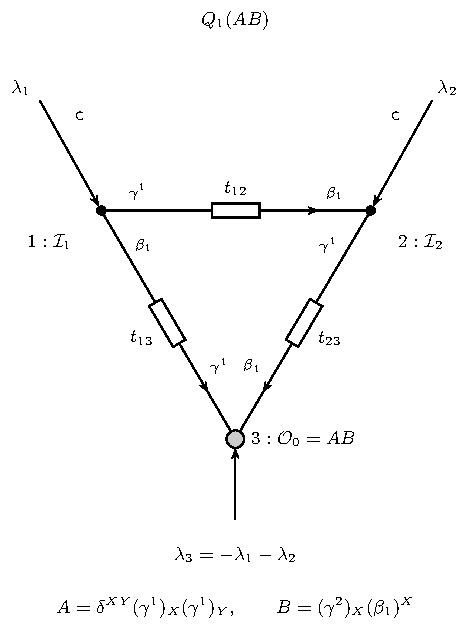
\includegraphics[width=0.52\linewidth,height=.44\textheight,keepaspectratio]{figures/circuits/graviton_Q1.pdf}
\caption{The circuit for the one-loop cross-contraction of the scalar and fermion gravitons. The resistors have resistances $t_{ij}$; the source currents $\lambda_1,\lambda_2$ record derivatives on the output ghost fields in $Q_1(AB)$.}
\label{fig:graviton-cross}
\end{figure}


The marked triangle of Figure~\ref{fig:graviton-dressing} gives the one-loop term of the quantum product:
\begin{equation}\label{eq:2.65}
\begin{aligned}
\mathcal O_1
&=\{\mathcal I,A,B\}^{\gamma,0}\\
&={\frac{i}{8\pi^2}}
{2(ig)(-1)}
{\frac12}
{\frac14}
C_D{}^{XY}(\partial_{+\dot a}\mathsf c^D)
(\partial_+{}^{\dot a}(\gamma^1)_X)(\gamma^2)_Y\\
&=\frac{g}{32\pi^2}C_D{}^{XY}(\partial_{+\dot a}\mathsf c^D)
(\partial_+{}^{\dot a}(\gamma^1)_X)(\gamma^2)_Y.
\end{aligned}
\end{equation}
\begin{figure}[H]
\centering
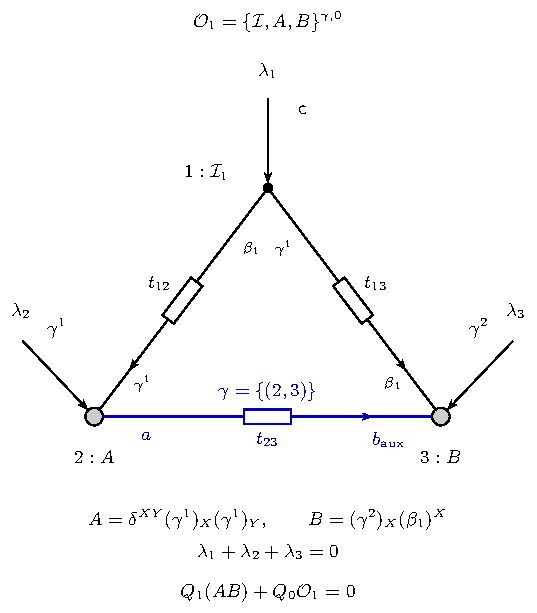
\includegraphics[width=0.52\linewidth,height=.44\textheight,keepaspectratio]{figures/circuits/graviton_dressing.pdf}
\caption{The marked triangle circuit giving the one-loop term of the quantum product of the two gravitons. Its resistances are $t_{12},t_{13},t_{23}$, with the auxiliary edge $23$ in blue. Applying $Q_0$ to its output fields cancels $Q_1(AB)$.}
\label{fig:graviton-dressing}
\end{figure}


To evaluate its classical variation, use
\begin{equation}\label{eq:scalarfermionrules}
\begin{aligned}
Q_0\mathsf c^D&=-\frac g2C^D{}_{EF}\mathsf c^E\mathsf c^F,\\
Q_0(\gamma^I)_X&=-gC_{XE}{}^F\mathsf c^E(\gamma^I)_F,\\
Q_0\partial_{+\dot a}(\gamma^I)_X
&=-gC_{XE}{}^F\bigl[
(\partial_{+\dot a}\mathsf c^E)(\gamma^I)_F
+\mathsf c^E\partial_{+\dot a}(\gamma^I)_F\bigr].
\end{aligned}
\end{equation}
The graded Leibniz rule expands $Q_0\mathcal O_1$ into
\begin{equation}\label{eq:scalarfermionexpand}
\begin{aligned}
Q_0\mathcal O_1={}&\frac{g^2}{32\pi^2}C_D{}^{XY}\Bigl[
-C^D{}_{EF}(\partial_{+\dot a}\mathsf c^E)\mathsf c^F
(\partial_+{}^{\dot a}(\gamma^1)_X)(\gamma^2)_Y\\
&+C_{XE}{}^F(\partial_{+\dot a}\mathsf c^D)
(\partial_+{}^{\dot a}\mathsf c^E)(\gamma^1)_F(\gamma^2)_Y\\
&+C_{XE}{}^F(\partial_{+\dot a}\mathsf c^D)\mathsf c^E
(\partial_+{}^{\dot a}(\gamma^1)_F)(\gamma^2)_Y\\
&+C_{YE}{}^F(\partial_{+\dot a}\mathsf c^D)
(\partial_+{}^{\dot a}(\gamma^1)_X)\mathsf c^E(\gamma^2)_F
\Bigr].
\end{aligned}
\end{equation}
The first, third and fourth lines cancel by invariance of $C_{DXY}$,
\begin{equation}
C_{RX}{}^TC_{TYZ}+C_{RY}{}^TC_{XTZ}+C_{RZ}{}^TC_{XYT}=0.
\end{equation}
The remaining term is

\begin{equation}\label{eq:2.66}
\begin{aligned}
Q_0\mathcal O_1
&=\frac{g^2}{32\pi^2}
C_D{}^{XY}C_{XE}{}^F(\gamma^1)_F(\gamma^2)_Y
(\partial_{+\dot a}\mathsf c^D)(\partial_+{}^{\dot a}\mathsf c^E)\\
&=-\frac{g^2}{32\pi^2}
C^X{}_{RD}C^{YR}{}_{E}(\gamma^1)_X(\gamma^2)_Y
(\partial_{+\dot a}\mathsf c^D)(\partial_+{}^{\dot a}\mathsf c^E)\\
&=-Q_1\mathcal O_0.
\end{aligned}
\end{equation}

The one-loop term of the quantum product therefore cancels the variation of the ordinary
product of the two gravitons. The component degrees
$\deg_\theta\mathcal O_0=5$ and $\deg_\theta\mathcal O_1=2$ give
\begin{equation}\label{eq:finiteexample}
\begin{gathered}
\mathcal O=A\star B=\mathcal O_0+\hbar\mathcal O_1,\qquad
Q_{n\ge2}\mathcal O_0=Q_{n\ge1}\mathcal O_1=0,\\
\mathbf Q\mathcal O
=\hbar(Q_1\mathcal O_0+Q_0\mathcal O_1)=0.
\end{gathered}
\end{equation}
The displayed one-loop completion is the full perturbative product.

\subsection{Homotopy transfer and successive obstructions}
\label{sec:homotopy-transfer}

The quantum differential acts on a completed representative
$\mathcal O=\sum_{r\ge0}\hbar^r\mathcal O_r$ through
\begin{equation}\label{eq:liftingequations}
\begin{aligned}
Q_0\mathcal O_0&=0,\\
Q_0\mathcal O_1&=-Q_1\mathcal O_0,\\
Q_0\mathcal O_2&=-Q_2\mathcal O_0-Q_1\mathcal O_1,\\
\sum_{k=0}^{r}Q_k\mathcal O_{r-k}&=0.
\end{aligned}
\end{equation}
\paragraph{Successive contractions.}
Let $E_0$ be the complex of holomorphic local operators and set
$d_0=Q_0$. The pages are iterated cohomologies,
\begin{equation}\label{eq:page-iterated}
\begin{gathered}
E_1=H(Q_0),\qquad
E_2=H\bigl(H(Q_0),d_1\bigr),\qquad
E_3=H\bigl(H(H(Q_0),d_1),d_2\bigr),\\
\ldots,\qquad
E_{r+1}=H(E_r,d_r),
\end{gathered}
\end{equation}
each the quotient of the kernel of $d_r$ by its image. The first
differential is $d_1[\mathcal O_0]_1=[Q_1\mathcal O_0]_1$, and
$Q_1^2=-(Q_0Q_2+Q_2Q_0)$ gives $d_1^2=0$. From the second page on,
$d_r$ is not the class of $Q_r$. For a class of $E_2$, with
$Q_0\mathcal O_0=0$ and $Q_0\mathcal O_1=-Q_1\mathcal O_0$,
\begin{equation}\label{eq:Q2-not-closed}
Q_0Q_2\mathcal O_0=-Q_1^2\mathcal O_0=Q_1Q_0\mathcal O_1,
\end{equation}
which need not vanish, while $Q_2\mathcal O_0+Q_1\mathcal O_1$ is closed
\eqref{eq:d2closure}. Each $d_r$ is transferred from $\mathbf Q$ through
the contractions of the earlier pages, and $d_r^2=0$ on $E_r$
\eqref{eq:page-transfer-identities}. Choose an inclusion $i_r:E_{r+1}\to E_r$ of cohomology
representatives, a projection $\pi_r:E_r\to E_{r+1}$, and a homotopy
$h_r:E_r\to E_r$ of degree $-1$, satisfying
\begin{equation}\label{eq:page-contraction}
\begin{gathered}
\pi_ri_r=1,\qquad d_ri_r=\pi_rd_r=0,\qquad
d_rh_r+h_rd_r=1-i_r\pi_r,\\
h_ri_r=\pi_rh_r=h_r^2=0.
\end{gathered}
\end{equation}
These maps separate representatives from exact pairs.

Write $\mathbf Q^{(0)}=\mathbf Q$. The differential
$\mathbf Q^{(r)}$ on $E_r[[\hbar]]$ has constant term $d_r$.
Its transferred differential and corrected maps are
\begin{equation}\label{eq:page-transfer}
\begin{aligned}
i_r(\hbar)
&=\bigl[1+h_r(\mathbf Q^{(r)}-d_r)\bigr]^{-1}i_r,\\
\pi_r(\hbar)
&=\pi_r\bigl[1+(\mathbf Q^{(r)}-d_r)h_r\bigr]^{-1},\\
h_r(\hbar)
&=\bigl[1+h_r(\mathbf Q^{(r)}-d_r)\bigr]^{-1}h_r,\\
\mathbf Q^{(r+1)}
&=\frac1\hbar\pi_r(\mathbf Q^{(r)}-d_r)i_r(\hbar),
&d_{r+1}&=\left.\mathbf Q^{(r+1)}\right|_{\hbar=0}.
\end{aligned}
\end{equation}
The inverses are formal geometric series; their order-$\hbar^k$
coefficients contain finitely many terms. For example, the inclusion
satisfies
\begin{equation}\label{eq:page-chain-derivation}
\begin{aligned}
i_r(\hbar)
&=i_r-h_r(\mathbf Q^{(r)}-d_r)i_r(\hbar),\\
\mathbf Q^{(r)}i_r(\hbar)
&=\hbar i_r\mathbf Q^{(r+1)}
-h_r(\mathbf Q^{(r)}-d_r)\mathbf Q^{(r)}i_r(\hbar).
\end{aligned}
\end{equation}
The second line follows from
$d_rh_r=1-i_r\pi_r-h_rd_r$ and
$(\mathbf Q^{(r)})^2=d_r^2=0$.
Multiplying by the inverse in \eqref{eq:page-transfer}, and applying
the corresponding calculation to the projection and homotopy, gives
\begin{equation}\label{eq:page-transfer-identities}
\begin{aligned}
\mathbf Q^{(r)}i_r(\hbar)
&=\hbar i_r(\hbar)\mathbf Q^{(r+1)},\\
\pi_r(\hbar)\mathbf Q^{(r)}
&=\hbar\mathbf Q^{(r+1)}\pi_r(\hbar),\\
\mathbf Q^{(r)}h_r(\hbar)+h_r(\hbar)\mathbf Q^{(r)}
&=1-i_r(\hbar)\pi_r(\hbar),\\
\pi_r(\hbar)i_r(\hbar)&=1,
&\bigl(\mathbf Q^{(r+1)}\bigr)^2&=0.
\end{aligned}
\end{equation}
Thus each new obstruction is itself a differential.

\paragraph{The first obstruction maps.}
Writing $[\hbar^k]$ for the coefficient of $\hbar^k$, the first
transfer has coefficients
\begin{equation}\label{eq:first-page-series}
\begin{aligned}
[\hbar^0]\mathbf Q^{(1)}&=\pi_0Q_1i_0,\\
[\hbar]\mathbf Q^{(1)}&=\pi_0(Q_2-Q_1h_0Q_1)i_0,\\
[\hbar^2]\mathbf Q^{(1)}&=\pi_0\bigl(
Q_3-Q_2h_0Q_1-Q_1h_0Q_2
+Q_1h_0Q_1h_0Q_1\bigr)i_0.
\end{aligned}
\end{equation}
In particular,
\begin{equation}\label{eq:page-differentials}
\begin{aligned}
d_1&=\pi_0Q_1i_0,\\
d_2&=\pi_1\pi_0(Q_2-Q_1h_0Q_1)i_0i_1,\\
d_3&=\pi_2\pi_1\Bigl(
[\hbar^2]\mathbf Q^{(1)}
-([\hbar]\mathbf Q^{(1)})h_1
 ([\hbar]\mathbf Q^{(1)})\Bigr)i_1i_2.
\end{aligned}
\end{equation}
The second term in $d_2$ is the contribution of the first correction to
the representative. To see it directly, take
$\mathcal O_0=i_0i_1a$ with $a\in E_2$, and choose
$\mathcal O_1=-h_0Q_1\mathcal O_0$. Then
\begin{equation}\label{eq:d2closure}
\begin{aligned}
Q_0\mathcal O_1
&=-(1-i_0\pi_0)Q_1\mathcal O_0=-Q_1\mathcal O_0,\\
Q_0(Q_2\mathcal O_0+Q_1\mathcal O_1)
&=-Q_1^2\mathcal O_0-Q_1Q_0\mathcal O_1=0,\\
\pi_1\pi_0(Q_2\mathcal O_0+Q_1\mathcal O_1)&=d_2a.
\end{aligned}
\end{equation}
Equivalently, with $[\cdot]_r$ denoting a class on $E_r$,
\begin{equation}\label{eq:d2}
d_2[\mathcal O_0]_2
=[Q_2\mathcal O_0+Q_1\mathcal O_1]_2.
\end{equation}
Changing $\mathcal O_1$ by a classical cocycle changes the projected
obstruction by a $d_1$ boundary.

\paragraph{Corrected representatives.}
For a class $a\in E_3$, the vanishing of $d_2i_2a$ determines
corrections through two loops. One choice requiring only
$Q_0,Q_1,Q_2$ is
\begin{equation}\label{eq:two-loop-representative-transfer}
\begin{aligned}
\mathcal O_0&=i_0i_1i_2a,\\
\mathcal O_1
&=-h_0Q_1\mathcal O_0
-i_0h_1\pi_0(Q_2-Q_1h_0Q_1)\mathcal O_0,\\
\mathcal O_2&=-h_0(Q_2\mathcal O_0+Q_1\mathcal O_1).
\end{aligned}
\end{equation}
Indeed,
\begin{equation}\label{eq:two-loop-representative-projection}
\begin{aligned}
\pi_0(Q_2\mathcal O_0+Q_1\mathcal O_1)
&=(1-d_1h_1)\pi_0(Q_2-Q_1h_0Q_1)\mathcal O_0\\
&=i_1\pi_1\pi_0(Q_2-Q_1h_0Q_1)\mathcal O_0=0.
\end{aligned}
\end{equation}
The term with $h_1d_1$ vanishes by the coefficient of $\hbar$ in
$(\mathbf Q^{(1)})^2=0$. Equation~\eqref{eq:page-contraction}
then verifies all three closure equations in
\eqref{eq:liftingequations}.

At every page the same construction gives
\begin{equation}\label{eq:page-representative-chain}
\mathbf Q\,i_0(\hbar)\cdots i_{r-1}(\hbar)
=\hbar^r i_0(\hbar)\cdots i_{r-1}(\hbar)\mathbf Q^{(r)}.
\end{equation}
For $a\in E_{r+1}$, choose $\mathcal O_s$ as the coefficient of
$\hbar^s$ in $i_0(\hbar)\cdots i_{r-1}(\hbar)i_ra$. Then
\begin{equation}\label{eq:2.75}
\sum_{k=0}^{s}Q_k\mathcal O_{s-k}=0\quad(0\le s\le r),
\qquad
d_{r+1}[\mathcal O_0]_{r+1}
=\left[\sum_{k=1}^{r+1}Q_k\mathcal O_{r+1-k}\right]_{r+1}.
\end{equation}
Each successive inclusion also fixes the lower-page cocycle terms
that may be added to the earlier corrections.

\paragraph{Products and classical representatives.}
Suppose the homogeneous operators $A=\sum_{s<r}\hbar^sA_s$ and
$B=\sum_{s<r}\hbar^sB_s$ satisfy the closure equations through order
$r-1$. Write $\mathcal O_s=[\hbar^s](A\star B)$.
The leading term is $\mathcal O_0=A_0B_0$. Taking coefficients
in \eqref{eq:chain} gives
\begin{equation}\label{eq:2.77}
\begin{gathered}
\sum_{k=0}^{s}Q_k\mathcal O_{s-k}=0\qquad(0\le s<r),\\
\begin{aligned}
Q_0\mathcal O_r+\sum_{k=1}^{r}Q_k\mathcal O_{r-k}
={}&\Bigl(\sum_{k=1}^{r}Q_kA_{r-k}\Bigr)B_0\\
&+(-1)^{|A_0|}A_0\Bigl(\sum_{k=1}^{r}Q_kB_{r-k}\Bigr).
\end{aligned}
\end{gathered}
\end{equation}
Passing to $E_r$ gives
\begin{equation}\label{eq:2.78}
\begin{aligned}
[A_0]_r[B_0]_r&=[A_0B_0]_r,\\
d_r([A_0]_r[B_0]_r)
&=(d_r[A_0]_r)[B_0]_r
+(-1)^{|A_0|}[A_0]_r(d_r[B_0]_r).
\end{aligned}
\end{equation}
Starting from multiplication on $H(Q_0)$, this identity gives an
associative graded-commutative product on each successive page.
The transfer incorporates the higher corrections into $d_r$; kernels,
images, linear independence and product relations can then be computed
on the corresponding subquotients of classical representatives.

\paragraph{Higher differentials on the graviton part.}
\label{sec:graviton-dr}
Applying the projection identity in \eqref{eq:page-transfer-identities}
on successive pages gives
\begin{equation}\label{eq:graviton-dr}
\pi_{r-1}(\hbar)\cdots\pi_0(\hbar)\,\mathbf Q
=\hbar^r\,\mathbf Q^{(r)}\,\pi_{r-1}(\hbar)\cdots\pi_0(\hbar).
\end{equation}
If $\mathbf Q\mathcal O=0$, dividing \eqref{eq:graviton-dr} applied to
$\mathcal O$ by $\hbar^r$ gives
$\mathbf Q^{(r)}\pi_{r-1}(\hbar)\cdots\pi_0(\hbar)\mathcal O=0$. Its
constant term is $d_r\pi_{r-1}\cdots\pi_0\mathcal O_0$, and by induction
on $r$ the projection $\pi_{r-1}\cdots\pi_0\mathcal O_0$ is the class
$[\mathcal O_0]_r$. Hence a class with a closed completion satisfies
\begin{equation}\label{eq:graviton-dr-zero}
d_r[\mathcal O_0]_r=0\qquad(r\ge1).
\end{equation}
By Theorem~\ref{thm:multigraviton-closure}, every $d_r$ with $r\ge1$
vanishes on the graviton part. On classes of cohomological degree $k$,
the rank of $d_r$ is the dimension of the space of degree-$k$ classical
classes that survive to $E_r$, including those that vanish there, modulo
those that survive to $E_{r+1}$. Every class of the graviton part survives
to every page. In each charge sector, the ranks of all $d_r$ with $r\ge1$
on degree $k$ therefore add up to at most the number of fortuitous classes
of degree $k$. These classes are sparse among the
classical classes known so far \cite{microstates,KKLP}, so the successive
differentials are extremely sparse on the known cohomology.

A closed completion can become a quantum coboundary.
For completed operators satisfying
\begin{equation}\label{eq:incoming-exactness}
\mathbf Q X=\hbar^r\mathcal O,\qquad
\mathbf Q\mathcal O=0,
\qquad
\mathcal O=\mathbf Q(\hbar^{-r}X),
\end{equation}
the last equality holds after inverting $\hbar$.
Over formal power series, the first equality records a class
annihilated by $\hbar^r$. The successive pages record these $d_r$-exact classes at their respective
orders in $\hbar$.

\paragraph{Finite-dimensional computation.}
Fix the conserved charges and the gauge-group rank in a sector with
finitely many local monomials. In each cohomological
degree, expand the gauge-invariant local operators in a basis of component
fields and holomorphic derivatives, imposing the graded field relations and
the trace identities at that rank. Applying \eqref{eq:2.8} to each basis
element gives the columns of $Q_n$. Retain the adjacent cohomological degrees
that supply the images and kernels. The simplex integrals give exact
coefficients; the resulting matrices can be reduced over the coefficient
field containing the couplings and the constants in \eqref{eq:2.8}.

The computation proceeds page by page. The input on $E_r$ is a basis of
representatives in each degree, completed through order $r-1$ by
$i_0(\hbar)\cdots i_{r-1}(\hbar)$, together with the matrix of $d_r$ from
\eqref{eq:page-transfer}. The output is a contraction $(i_r,\pi_r,h_r)$,
hence $E_{r+1}$, the matrix of $d_{r+1}$ and the next corrections.
Let $d_r^k:E_r^k\to E_r^{k+1}$ denote the differential in
cohomological degree $k$. Choose the columns of $B_r^k$ to span
$\operatorname{im}d_r^{k-1}$, extend them by the columns of $H_r^k$ to a basis
of $\ker d_r^k$, and choose $L_r^k$ so that
\begin{equation}\label{eq:page-basis-splitting}
d_r^kL_r^k=B_r^{k+1},\qquad
(B_r^k\;H_r^k\;L_r^k)\ \text{is invertible}.
\end{equation}
The contraction is then
\begin{equation}\label{eq:page-matrix-contraction}
\begin{aligned}
i_r^k&=H_r^k,\\
\pi_r^k&=(0\;1\;0)(B_r^k\;H_r^k\;L_r^k)^{-1},\\
h_r^k&=L_r^{k-1}(1\;0\;0)(B_r^k\;H_r^k\;L_r^k)^{-1}.
\end{aligned}
\end{equation}
Here the block $1$ is the identity on the indicated group of columns. Thus
\begin{equation}\label{eq:page-matrix-checks}
\begin{gathered}
d_r^{k-1}h_r^k+h_r^{k+1}d_r^k=1-i_r^k\pi_r^k,
\qquad \pi_r^ki_r^k=1,\\
h_r^{k-1}h_r^k=0,\qquad h_r^ki_r^k=0,
\qquad \pi_r^{k-1}h_r^k=0.
\end{gathered}
\end{equation}
The inclusion $i_r$ is the natural embedding of the chosen
representatives. The freedom lies in the complements $H_r^k$ and $L_r^k$,
which fix $\pi_r$ and $h_r$. Three choices are typical.

In the \emph{pivot splitting}, used in the calculations of
Section~\ref{sec:applications}, the monomials are ordered and the columns
of $d_r^k$ are eliminated in exact rational arithmetic, the first monomial
of each reduced column being its pivot. The basis vectors whose images
supply new pivots form $L_r^k$, and their images form $B_r^{k+1}$; the
linear dependencies found in the elimination span $\ker d_r^k$, and the
kernel vectors independent modulo $B_r^k$ form $H_r^k$. Then $\pi_r$
reduces a vector against the pivot columns of
$(B_r^k\;H_r^k\;L_r^k)$ and keeps its $H_r^k$ coordinates, and $h_r$
replaces its $B_r^k$ coordinates by the same combination of the preimages
$L_r^{k-1}$. For the largest sectors the pivot columns can be selected
modulo a prime after a random linear projection of the rows; the
coefficients are then recomputed over $\mathbb Q$ on the selected columns,
and the result is checked by applying $Q_0$ exactly.

In the \emph{orthogonal splitting}, with the monomials orthonormal,
$H_r^k=\ker d_r^k\cap(\operatorname{im}d_r^{k-1})^\perp$, $\pi_r$ is the
orthogonal projection, and $h_r$ is the Moore--Penrose pseudoinverse of
$d_r$; it does not depend on an ordering of the monomials, but its matrices
are dense.

When a pair of letters decouples from the others under $Q_0$, as
$Q_0\beta^s=-m\gamma_s'$ and $Q_0\gamma_s'=0$ in the shifted fields
\eqref{eq:massshift} of Section~\ref{sec:SQEDlift}, the homotopy of that
pair has a \emph{closed form}: the odd derivation that replaces each
factor $\gamma_s'$, with its derivatives, by the same derivative of
$-\beta^s/m$, divided by the number of letters $\gamma_s',\beta^s$; the
projection sets these letters to zero.

Two contractions $(i_r,\pi_r,h_r)$ and $(i_r',\pi_r',h_r')$ of the same page
give conjugate transferred differentials. By
\eqref{eq:page-transfer-identities},
\begin{equation}\label{eq:page-choice}
\hbar\,\pi_r'(\hbar)i_r(\hbar)\,\mathbf Q^{(r+1)}
=\pi_r'(\hbar)\,\mathbf Q^{(r)}\,i_r(\hbar)
=\hbar\,\mathbf Q'^{(r+1)}\,\pi_r'(\hbar)i_r(\hbar),
\end{equation}
and the constant term $\pi_r'i_r$, which sends a representative to its
class in the other splitting, is invertible on $E_{r+1}$. The pages, the
ranks of all $d_s$, and the vanishing of a given class are therefore
independent of the choices. At each step, check the nilpotence of the
transferred differential and its intertwining identity with $i_r(\hbar)$
through the retained order in $\hbar$.

In practice $\pi_r$ and $h_r$ are applied by reduction against the stored
pivot columns rather than formed as matrices. On the first page a single
elimination gives $\ker d_1$ together with first corrections: reducing the
columns $Q_1\mathcal O_0$ of the representatives against the columns $Q_0v$,
with $v$ running over the basis of the first-correction sector, returns every
combination with $Q_1\mathcal O_0+Q_0\mathcal O_1=0$. On the second page,
\begin{equation}\label{eq:d2-quotient-test}
d_2[\mathcal O_0]_2=0
\quad\Longleftrightarrow\quad
Q_2\mathcal O_0+Q_1\mathcal O_1\in\operatorname{im}Q_0+Q_1\ker Q_0,
\end{equation}
with $\ker Q_0$ taken in the first-correction sector, which covers every
change of $\mathcal O_1$ by a classical cycle. A rational linear functional
that vanishes on $\operatorname{im}Q_0+Q_1\ker Q_0$ but not on
$Q_2\mathcal O_0+Q_1\mathcal O_1$ certifies $d_2[\mathcal O_0]_2\ne0$, as in
Section~\ref{sec:SQEDlift}.

The number of surviving classes in degree $k$ is
\begin{equation}\label{eq:page-rank}
\dim E_{r+1}^k
=\dim E_r^k-\operatorname{rank}d_r^k
              -\operatorname{rank}d_r^{k-1}.
\end{equation}
For closed candidate columns $v_1,\ldots,v_m\in\ker d_r^k$, their classes span
a space of dimension
\begin{equation}\label{eq:page-independence}
\operatorname{rank}(B_r^k\;v_1\;\cdots\;v_m)
-\operatorname{rank}B_r^k
=\operatorname{rank}\bigl[\pi_r^k(v_1\;\cdots\;v_m)\bigr].
\end{equation}
This tests both linear relations and exactness on the current
page. Representatives through the computed order are reconstructed by the
successive inclusions $i_0(\hbar)\cdots i_r(\hbar)$.

The algorithm does not require the quantum product. On every page the
class of $A\star B$, whose leading term is $A_0B_0$, is
$[A_0]_r[B_0]_r=[A_0B_0]_r$ by \eqref{eq:2.78}: products of classes are
obtained by multiplying classical representatives and reducing on $E_r$,
and $d_r$ acts on them by the Leibniz rule.
\paragraph{Derivative grading.}
A monomial has two holomorphic derivative totals: its numbers of
$\partial_{+\dot+}$ and $\partial_{+\dot-}$ derivatives. Every current
is linear in the injected currents, and the current form in
\eqref{eq:operatope} has degree $n$ in each dotted component. For each
fixed $\dot a$ the kernel of an $n$-loop graph therefore
satisfies
\begin{equation}\label{eq:derivative-homogeneity}
\mathcal I_\Gamma^{\mathrm{raw\ cut}}
\bigl(\lambda_{v,+\dot a}\mapsto c\lambda_{v,+\dot a};\,
z_e^{+\dot a}\mapsto c^{-1}z_e^{+\dot a}\bigr)
=c^n\,\mathcal I_\Gamma^{\mathrm{raw\ cut}}(\lambda;z),
\qquad c>0.
\end{equation}
Powers of $\lambda_{v,+\dot a}$ become derivatives of output letters
and powers of $z_e^{+\dot a}$ remove input derivatives, so each $Q_n$
adds $n$ derivatives in each holomorphic direction, as observed for pure gauge theory in \cite[Equations (3.44)--(3.45)]{semichiral}. The classical
differential $Q_0$ preserves both totals, and the contractions
$(i_r,\pi_r,h_r)$ can be chosen homogeneous. By \eqref{eq:page-transfer},
every term of $d_r$ then adds $r$ derivatives in each direction.

\begin{lemma}\label{lem:derivative-grading}
A class can be $d_r$-exact only if both derivative totals of
its leading representative are at least $r$. In particular, a class
whose leading representative has no holomorphic derivatives is
$d_r$-exact for no $r\ge1$.
\end{lemma}
\begin{proof}
A preimage under $d_r$ would have both totals lowered by $r$, and
they must be nonnegative.
\end{proof}
The $n$ loop currents of each dotted component are linear in the injected currents, which act as derivatives on the output letters; a differential on the $r$th page therefore raises each derivative total by $r$, and a class without derivatives cannot be its image.


\section{Tests of lifting beyond one loop}
\label{sec:applications}

The obstruction equations of Section~\ref{sec:lifting} decide whether loop corrections beyond one loop lift classes that survive the one-loop differential, a question left open in \cite[Section 1]{BK}. A classical cocycle survives at every perturbative order if it is not classically exact and admits a closed completion that is a quantum coboundary at no positive loop order; by Lemma~\ref{lem:derivative-grading}, the last condition holds for a leading representative without holomorphic derivatives. In massive SQED the answer is positive: Section~\ref{sec:SQEDlift} exhibits a class that survives one loop and is lifted at two loops. Every other class we test survives at every perturbative order. In the complete low-letter sectors of $\mathcal N=4$ $SU(2)$ and $SU(3)$ theory treated in Section~\ref{sec:finite-sectors}, every classical class is a multi-graviton completed by Theorem~\ref{thm:multigraviton-closure}. Section~\ref{sec:fortuitous} completes the threshold fortuitous class of $\mathcal N=4$ $SU(2)$ theory, which this theorem does not cover, together with its graviton-dressed descendants; for the descendant carrying holomorphic derivatives, an explicit calculation excludes $d_1$-exactness. Section~\ref{sec:quartic-fortuitous} completes a graviton square and a non-graviton class of a quartic deformation with the spider kernels.

\subsection{A two-loop lifting example: massive SQED with a cubic superpotential}
\label{sec:SQEDlift}

Consider a $U(1)$ gauge theory with two chiral multiplets of charges $+1,-1$ and a neutral chiral multiplet. Its interaction is

\begin{equation}\label{eq:3.11}
\mathcal I=ig\mathsf c(\gamma_+\beta^+-\gamma_-\beta^-)+\frac m2\gamma_s^2+y\gamma_s\gamma_+\gamma_-,\qquad my\ne0,
\end{equation}

Here $m$ is the mass of the neutral multiplet and $y$ is the cubic superpotential coefficient. We exhibit a gauge-invariant cocycle $\mathcal O_0$ that survives the one-loop differential and has the nonzero second obstruction \eqref{eq:SQEDlift}. The calculation has five steps: the exact elimination of the massive pair, the source and its classical closure, the one-loop action and a first correction, the combined second-order residual, and its class in the finite obstruction quotient.

\paragraph{The massive pair.}
The neutral mass can be included exactly before computing the obstruction quotient. In the twisted BV complex, a canonical change of fields isolates a massive pair. The shifts
\begin{equation}\label{eq:massshift}
\gamma_s'=\gamma_s+\frac ym\gamma_+\gamma_-,\qquad
\beta^{+\prime}=\beta^+-\frac ym\gamma_-\beta^s,\qquad
\beta^{-\prime}=\beta^--\frac ym\gamma_+\beta^s
\end{equation}
complete the square and preserve the cotangent pairing:
\begin{equation}\label{eq:masssquare}
\frac m2\gamma_s^2+y\gamma_s\gamma_+\gamma_-
=\frac m2(\gamma_s')^2-\frac{y^2}{2m}(\gamma_+\gamma_-)^2.
\end{equation}
The pair $Q_0\beta^s=-m\gamma_s'$, $Q_0\gamma_s'=0$ is contractible. The exact classical effective superpotential is
\begin{equation}
\bar W_{\mathrm{eff}}=-\frac{y^2}{2m}(\gamma_+\gamma_-)^2,
\qquad\bar W_{\mathrm{eff}}^{++--}=-\frac{2y^2}{m}.
\end{equation}
The superscript $++--$ denotes two derivatives with respect to each of $\gamma_+$ and $\gamma_-$. In the transfer formula below, $Q_n$ is expressed in the shifted fields before eliminating the massive pair. The projection $\pi$ sets $\gamma_s',\beta^s$ and their derivatives to zero; $\iota$ includes the light-field complex and $h$ contracts the massive pair. Expanding the homotopy-transfer series gives

\begin{equation}\label{eq:3.15}
\begin{aligned}
Q_0h+hQ_0&=1-\iota\pi,\\
Q_{1,\mathrm{eff}}&=\pi Q_1\iota,\\
Q_{2,\mathrm{eff}}&=\pi Q_2\iota-
{\pi Q_1hQ_1\iota}.
\end{aligned}
\end{equation}

The term $-\pi Q_1hQ_1\iota$ records a one-loop action into the massive pair followed by a second one-loop action back to the light fields. We compute the representative corrections in the full theory and use this transfer to form the finite obstruction quotient.

\paragraph{The source.}
For $gmy\ne0$, the following gauge-invariant cocycle survives the first obstruction map. Its second obstruction will be a cubic polynomial in derivatives of the meson $\gamma_+\gamma_-$:
\begin{equation}\label{eq:SQEDsource}
\begin{aligned}
\mathcal O_0=ig\Big[&\beta^+\beta^-\mathsf b^2
+\frac ym(\gamma_-\beta^--\gamma_+\beta^+)\beta^s\mathsf b^2\\
&+\frac{y^2}{3m\,ig}\gamma_+\gamma_-\mathsf b^3\Big]
\partial_{+\dot a}\mathsf c .
\end{aligned}
\end{equation}
The free index $\dot a$ labels its two dotted spinor components. Since $Q_0\mathsf c=0$ in this abelian theory, classical closure follows from the cancellation of the three variations
\begin{equation}\label{eq:SQEDclosure}
\begin{aligned}
Q_0(\beta^+\beta^-\mathsf b^2)
&=y\gamma_s(\gamma_+\beta^+-\gamma_-\beta^-)\mathsf b^2,\\
Q_0\big[(\gamma_-\beta^--\gamma_+\beta^+)\beta^s\mathsf b^2\big]
&=-(\gamma_+\beta^+-\gamma_-\beta^-)
(m\gamma_s+y\gamma_+\gamma_-)\mathsf b^2,\\
Q_0(\gamma_+\gamma_-\mathsf b^3)
&=3ig\gamma_+\gamma_-(\gamma_+\beta^+-\gamma_-\beta^-)\mathsf b^2.
\end{aligned}
\end{equation}
The shift \eqref{eq:massshift} takes \eqref{eq:SQEDsource} to the quartic representative
\begin{equation}
\mathcal O_0=ig\left(
\beta^{+\prime}\beta^{-\prime}\mathsf b^2
-\frac{\bar W_{\mathrm{eff}}^{++--}}{6ig}\gamma_+\gamma_-\mathsf b^3
\right)\partial_{+\dot a}\mathsf c,
\qquad
\bar W_{\mathrm{eff}}^{++--}=-\frac{2y^2}{m}.
\end{equation}
\paragraph{One loop.}
Writing the result in the shifted fields \eqref{eq:massshift}, the
one-loop triangle gives
\begin{equation}\label{eq:SQEDoneaction}
\begin{aligned}
(64\pi^2)Q_1\mathcal O_0
={}&2(ig)^3\Big\{
 \mathsf b\,\partial_{+\dot b}(\beta^{+\prime}\beta^{-\prime})
                    \partial_+{}^{\dot b}\mathsf c
 -(\partial_{+\dot b}\beta^{+\prime})\beta^{+\prime}\beta^{-\prime}
                    \partial_+{}^{\dot b}\gamma_+\\
&\quad+\beta^{+\prime}(\partial_{+\dot b}\beta^{-\prime})\beta^{-\prime}
                    \partial_+{}^{\dot b}\gamma_-
 +\frac ym(\partial_{+\dot b}\beta^s)\mathsf b
   (\beta^{-\prime}\gamma_--\beta^{+\prime}\gamma_+)
                    \partial_+{}^{\dot b}\mathsf c\\
&\quad-\frac ym(\partial_{+\dot b}\beta^s)\beta^{+\prime}\beta^{-\prime}
                    \partial_+{}^{\dot b}(\gamma_+\gamma_-)
 \Big\}\partial_{+\dot a}\mathsf c\\
&+2(ig)^2y\Big\{
 \mathsf b^2(\partial_{+\dot b}\mathsf c)
                    \partial_+{}^{\dot b}\gamma_s'
 -\mathsf b(\partial_{+\dot b}\gamma_s')
   \bigl(\beta^{+\prime}\partial_+{}^{\dot b}\gamma_+
        +\beta^{-\prime}\partial_+{}^{\dot b}\gamma_-\bigr)
 \Big\}\partial_{+\dot a}\mathsf c\\
&-\frac{2(ig)^2y^2}{m}\Big\{
 2\mathsf b^2(\partial_{+\dot b}\mathsf c)
                    \partial_+{}^{\dot b}(\gamma_+\gamma_-)
 +3\mathsf b(\beta^{+\prime}\gamma_+-\beta^{-\prime}\gamma_-)
       (\partial_{+\dot b}\gamma_+)\partial_+{}^{\dot b}\gamma_-\\
&\quad+\mathsf b\gamma_+\gamma_-
  \bigl[(\partial_{+\dot b}\beta^{+\prime})\partial_+{}^{\dot b}\gamma_+
       +(\partial_{+\dot b}\beta^{-\prime})\partial_+{}^{\dot b}\gamma_-\bigr]\\
&\quad+\frac ym\mathsf b\gamma_+\gamma_-
       (\partial_{+\dot b}\beta^s)\partial_+{}^{\dot b}(\gamma_+\gamma_-)
 \Big\}\partial_{+\dot a}\mathsf c .
\end{aligned}
\end{equation}
The one-loop variation is removed by solving $Q_0\mathcal O_1=-Q_1\mathcal O_0$. One explicit first correction is
\begin{equation}\label{eq:SQEDfirst}
\begin{aligned}
(64\pi^2)\mathcal O_1
={}&\frac23\left[(ig)^2\beta^{+\prime}\beta^{-\prime}
             +\frac{igy^2}{m}\mathsf b\gamma_+\gamma_-\right]\\
&\quad\times\Big[
 (\partial_{+\dot a}\partial_{+\dot b}\beta^{+\prime})
                                      \partial_+{}^{\dot b}\gamma_+
 -(\partial_{+\dot b}\beta^{+\prime})
                         \partial_{+\dot a}\partial_+{}^{\dot b}\gamma_+\\
&\qquad\quad
 -(\partial_{+\dot a}\partial_{+\dot b}\beta^{-\prime})
                                      \partial_+{}^{\dot b}\gamma_-
 +(\partial_{+\dot b}\beta^{-\prime})
                         \partial_{+\dot a}\partial_+{}^{\dot b}\gamma_-
 \Big]\\
&+\frac{2(ig)^2}{3}\mathsf b\Big\{
 \bigl[(\partial_{+\dot b}\beta^{+\prime})\beta^{-\prime}
       -\beta^{+\prime}\partial_{+\dot b}\beta^{-\prime}\bigr]
                         \partial_{+\dot a}\partial_+{}^{\dot b}\mathsf c\\
&\qquad\quad-
 \bigl[(\partial_{+\dot a}\partial_{+\dot b}\beta^{+\prime})\beta^{-\prime}
       -\beta^{+\prime}\partial_{+\dot a}\partial_{+\dot b}\beta^{-\prime}\bigr]
                                      \partial_+{}^{\dot b}\mathsf c
 \Big\}\\
&+\frac{8igy^2}{3m}\mathsf b
  \bigl(\beta^{+\prime}\partial_{+\dot a}\gamma_+
       +\beta^{-\prime}\partial_{+\dot a}\gamma_-\bigr)
  (\partial_{+\dot b}\gamma_+)\partial_+{}^{\dot b}\gamma_-\\
&+\frac{4igy^2}{3m}\mathsf b\Big[
 \beta^{+\prime}\gamma_-(\partial_{+\dot b}\gamma_+)
                         \partial_{+\dot a}\partial_+{}^{\dot b}\gamma_+
 -\beta^{-\prime}\gamma_+(\partial_{+\dot b}\gamma_-)
                         \partial_{+\dot a}\partial_+{}^{\dot b}\gamma_-
 \Big]\\
&+\frac{igy^2}{3m}\mathsf b^2\Big\{
 (\partial_{+\dot b}\mathsf c)
 \bigl(\gamma_-\partial_{+\dot a}\partial_+{}^{\dot b}\gamma_+
      -\gamma_+\partial_{+\dot a}\partial_+{}^{\dot b}\gamma_-\bigr)\\
&\qquad\quad+
 (\partial_{+\dot a}\partial_{+\dot b}\mathsf c)
 \bigl(\gamma_+\partial_+{}^{\dot b}\gamma_-
      -\gamma_-\partial_+{}^{\dot b}\gamma_+\bigr)
 +15(\partial_{+\dot a}\mathsf c)
       (\partial_{+\dot b}\gamma_+)\partial_+{}^{\dot b}\gamma_-
 \Big\}\\
&+\frac{(ig)^2y}{m}\Big\{
 \mathsf b^2(\partial_{+\dot a}\beta^s)
       (\partial_{+\dot b}\mathsf c)\partial_+{}^{\dot b}\mathsf c\\
&\qquad\quad-2\mathsf b(\partial_{+\dot b}\beta^s)
   \bigl(\beta^{+\prime}\partial_+{}^{\dot b}\gamma_+
        +\beta^{-\prime}\partial_+{}^{\dot b}\gamma_-\bigr)
                         \partial_{+\dot a}\mathsf c
 \Big\}.
\end{aligned}
\end{equation}
Its classical variation gives
\begin{equation}\label{eq:SQEDfirst-closure}
Q_0\mathcal O_1=-Q_1\mathcal O_0.
\end{equation}

\paragraph{The second obstruction.}
Thus $\mathcal O_0+\hbar\mathcal O_1$ is closed through one loop. At second order, both the direct two-loop action and the one-loop action on this correction enter:
\begin{equation}\label{eq:SQEDcochains}
d_2[\mathcal O_0]_2=[Q_2\mathcal O_0+Q_1\mathcal O_1]_2.
\end{equation}
The calculation uses the gauge charge, fermion number, field weight,
and the two holomorphic derivative totals. The field weights are
chosen so that every term in the interaction has weight four:
\begin{center}
\begin{tabular}{lrrr}
\toprule
Field & $U(1)$ charge & Fermion number & Field weight\\
\midrule
$\gamma_+$ & $1$ & $0$ & $1$\\
$\gamma_-$ & $-1$ & $0$ & $1$\\
$\beta^+$ & $-1$ & $1$ & $3$\\
$\beta^-$ & $1$ & $1$ & $3$\\
$\gamma_s$ & $0$ & $0$ & $2$\\
$\beta^s$ & $0$ & $1$ & $2$\\
$\mathsf b$ & $0$ & $0$ & $4$\\
$\mathsf c$ & $0$ & $1$ & $0$\\
\bottomrule
\end{tabular}
\end{center}
The parameters $m,y,g$ and holomorphic derivatives have field weight
zero. A monomial's derivative totals count its
$\partial_{+\dot+}$ and $\partial_{+\dot-}$ derivatives. Every BV
contraction removes field weight four. An $n$-loop fan has $n+1$
interaction vertices and $2n+1$ contractions, giving the weight shift
$4(n+1)-4(2n+1)=-4n$; its kernel adds derivative totals $(n,n)$.
The massive-pair homotopy preserves these degrees because
$\gamma_s'$ and $\beta^s$ both have field weight two.
The finite spaces below are taken in the relative gauge-invariant
complex of light fields: undifferentiated $\mathsf c$ implements gauge
transformations and is omitted from its representatives, while its
holomorphic derivatives remain. A second correction changes the residual
by a classical boundary. Changing the first correction by a classical
cycle changes the residual by its $Q_{1,\mathrm{eff}}$ image. These two
spaces supply the columns of the obstruction quotient.

\paragraph{The quotient test.}
For $\dot a=\dot+$, exact rational elimination gives:

\begin{center}
\begin{tabular}{lr}
\toprule
Space or map & Dimension or rank\\
\midrule
Odd source space, weight $14$, derivatives $(1,0)$ & $33$\\
Classical source cycles and boundaries & $18,\ 17$\\
First-correction space, weight $10$, derivatives $(2,1)$ & $365$\\
Classical cycles in the first-correction space & $180$\\
Second primitives, weight $6$, derivatives $(3,2)$ & $752$\\
Columns of $\operatorname{im}Q_0+Q_{1,\mathrm{eff}}\ker Q_0$ & $932$\\
Rank of these columns & $394$\\
Rank after adjoining the second obstruction & $395$\\
\bottomrule
\end{tabular}
\end{center}
The $18$ classical source cycles contain $17$ independent boundaries,
and $\mathcal O_0$ spans the remaining class. Its one-loop completion
and derivative totals $(1,0)$ give $[\mathcal O_0]_2\ne0$: a $d_1$-preimage
would have totals $(0,-1)$. In the target, the $752$ second
primitives and $180$ closed changes of the first correction give
$932$ columns of rank $394$. The obstruction supplies one more
independent column, so neither freedom cancels it.
The companion \href{run:SQED_two_loop_repro.zip}{\texttt{SQED\_two\_loop\_repro.zip}}\label{sec:SQEDcode}
contains the exact coefficients and executable verification code. It
regenerates the source and correction spaces, all $932$ quotient columns,
and verifies a rational linear functional $\ell$ on the obstruction target. For every second-order candidate $V$ and every
classical cycle $Z$ in the first-correction space, it obeys
\begin{equation}
\begin{gathered}
\ell(Q_0V)=0,\qquad
\ell(Q_{1,\mathrm{eff}}Z)=0\quad (Q_0Z=0),\\
\ell\pi(Q_2\mathcal O_0+Q_1\mathcal O_1)
=-\frac{16(ig)^2y^4}{m^2(64\pi^2)^2}.
\end{gathered}
\end{equation}
Reducing the projected residual in this quotient gives
\begin{equation}\label{eq:SQEDlift}
\begin{aligned}
d_2[\mathcal O_0]_2
&=-\frac{2(ig)^2y^4}{m^2(64\pi^2)^2}\Big[
\partial_{+\dot a}(\gamma_+\gamma_-)\\[-2pt]
&\qquad\times\partial_{+\dot b}\partial_{+\dot c}(\gamma_+\gamma_-)
\partial_+{}^{\dot b}\partial_+{}^{\dot c}(\gamma_+\gamma_-)
\Big]_2\ne0.
\end{aligned}
\end{equation}
The rank increase and the nonzero value of $\ell$ prove the last inequality.
This is the first example in our search whose lifting occurs at two loops:
$[\mathcal O_0]_2$ survives the one-loop differential, and
\eqref{eq:SQEDlift} removes it on the third page.

\subsection{Complete multi-graviton sectors in \texorpdfstring{$SU(2)$ and $SU(3)$}{SU(2) and SU(3)}}
\label{sec:finite-sectors}

In the sectors below every classical class is represented by a product
of single gravitons, so Theorem~\ref{thm:multigraviton-closure} supplies
its all-order completion by quantum multiplication. The sectors test
the representative equations and linear independence after quantum
corrections. Their representatives contain the two-letter single-graviton
class $(w_2)^I$ of \cite[Eq.~(2.14)]{KKLP}; in the present component
convention,
\begin{equation}\label{eq:w2}
(w_2)^I=\operatorname{Tr}\!\left(
\frac{\gamma^I\mathsf b}{ig}
-\frac12\varepsilon^{IJK}\beta_J\beta_K\right).
\end{equation}

For $SU(2)$, take all invariants without holomorphic derivatives,
with at most four letters and
$\deg_\theta-\#\text{letters}=3$.
The three flavour weights count the $\theta_I$ indices of the
superfield: $\gamma^I$ contributes index $I$, $\beta_I$ contributes
the two complementary indices, and $\mathsf b$ contributes all three.
The only blocks with nonzero classical cohomology have four letters.
Up to flavour permutation, their dimensions are
\begin{equation}
\begin{array}{c|rrrrr}
\text{flavour weight}&\text{invariants}&\dim\ker Q_0&
\dim\operatorname{im}Q_0&\dim H(Q_0)&\text{orbit size}\\\hline
(3,2,2)&13&4&1&3&3\\
(3,3,1)&5&2&1&1&3\\
(4,2,1)&3&1&0&1&6
\end{array}
\end{equation}
The last column counts distinct flavour permutations of each weight,
giving $3\cdot3+1\cdot3+1\cdot6=18$ classes. Restricting all fields
to a common Cartan subalgebra sets the commutators in $Q_0$ to zero,
so every classical boundary restricts to zero. The restrictions have
ranks $3,1,1$ on the three cohomology blocks, respectively; hence they
detect all eighteen independent classes. Five seeds generate their representatives
by permuting flavour labels with signs that preserve $\varepsilon^{IJK}$:
\begin{equation}
\begin{aligned}
\mathcal O_0^{(1)}&=-\operatorname{Tr}(\beta_2\gamma^1)(w_2)^2,\\
\mathcal O_0^{(2)}&=-\bigl[\operatorname{Tr}(\beta_2\gamma^2)
-\operatorname{Tr}(\beta_1\gamma^1)\bigr](w_2)^1,\\
\mathcal O_0^{(3)}&=-\operatorname{Tr}(\beta_3\gamma^1)(w_2)^3,\\
\mathcal O_0^{(4)}&=-\operatorname{Tr}(\beta_3\gamma^1)(w_2)^2,\\
\mathcal O_0^{(5)}&=-\operatorname{Tr}(\beta_3\gamma^1)(w_2)^1.
\end{aligned}
\end{equation}
Each seed is a product of two classical single-graviton traces, so
its quantum product is closed at every order. The representative
equations can also be solved directly. For the last seed,
$-\operatorname{Tr}(\beta_3\gamma^1)(w_2)^1$, the contractions between
its two factors are cancelled by the first correction
\begin{equation}\label{eq:su2-short-correction}
\begin{aligned}
\mathcal O_1^{(5)}=-\frac{i\epsilon^{\dot a\dot b}}{64\pi^2}C_A{}^{BC}
\Big[& (\beta_3)^A(\partial_{+\dot a}\gamma^1)_B
(\partial_{+\dot b}\gamma^1)_C\\
&-2(\partial_{+\dot a}\beta_3)^A(\gamma^1)_B
(\partial_{+\dot b}\gamma^1)_C\Big].
\end{aligned}
\end{equation}
All five seeds satisfy
\begin{equation}
\begin{gathered}
Q_1\mathcal O_0^{(j)}=-Q_0\mathcal O_1^{(j)}\ne0,\qquad
Q_2\mathcal O_0^{(j)}=Q_1\mathcal O_1^{(j)}=0,\\
\mathbf Q\bigl(\mathcal O_0^{(j)}+\hbar\mathcal O_1^{(j)}\bigr)=0.
\end{gathered}
\end{equation}
The source and first correction have component degrees $7$ and $4$.
After the displayed second-order cancellation, every term at order
$r\ge3$ has degree $7-3r<0$. Thus all eighteen completions end at
one loop. Cartan restriction proves their classical independence, and
Lemma~\ref{lem:derivative-grading} excludes $d_r$-exactness for $r\ge1$.

For $SU(3)$, all five-letter zero-jet invariants of flavour weight
$(3,3,2)$ give
\begin{equation}
\dim(\text{sources})=147,\qquad
\dim\ker Q_0=35,\qquad
\dim\operatorname{im}Q_0=26,\qquad
\dim H(Q_0)=9.
\end{equation}
The four-letter primitives supply the $26$ independent boundaries
inside the $35$ source cycles. All nine resulting classes are products
of a two-letter and a three-letter graviton trace, and their Cartan
restrictions have rank nine. Every class admits a completion through
second order. One example, whose first factor is $(w_2)^2$, is
\begin{equation}\label{eq:su3-example-source}
\mathcal O_0=\operatorname{Tr}\!\left(
\frac{\mathsf b\gamma^2}{ig}+\beta_1\beta_3\right)
\operatorname{Tr}(\beta_2\gamma^1\gamma^2-\beta_3\gamma^3\gamma^1).
\end{equation}
Its first and second corrections are displayed below. Here
$[X,Y]=XY-YX$ and
$\{X,Y\}=XY+YX$, with the field order as written:
\begin{align}\label{eq:su3-example-first}
\mathcal O_1=\frac{\epsilon^{\dot a\dot b}}{64\pi^2}
\operatorname{Tr}\Big\{
&(\partial_{+\dot b}\mathsf c)
[\partial_{+\dot a}\mathsf b,\gamma^1\gamma^2]\notag\\
&+ig(\partial_{+\dot b}\mathsf c)
\bigl(\{\gamma^1\beta_3,\partial_{+\dot a}\beta_1\}
+\{\gamma^2\beta_2-\beta_3\gamma^3,
\partial_{+\dot a}\beta_3\}\bigr)\notag\\
&+\gamma^1\gamma^2\bigl(
[\partial_{+\dot b}\gamma^1,\partial_{+\dot a}\beta_1]
-[\partial_{+\dot b}\gamma^2,\partial_{+\dot a}\beta_2]
+[\partial_{+\dot b}\gamma^3,\partial_{+\dot a}\beta_3]\bigr)\notag\\
&+2\gamma^1(\partial_{+\dot b}\gamma^2)
\bigl(-(\partial_{+\dot a}\gamma^2)\beta_2
+(\partial_{+\dot a}\beta_3)\gamma^3\bigr)\notag\\
&+\gamma^1\beta_3[\partial_{+\dot b}\gamma^2,\partial_{+\dot a}\gamma^3]
+2\gamma^1(\partial_{+\dot b}\beta_3)(\partial_{+\dot a}\gamma^2)\gamma^3\notag\\
&-(\partial_{+\dot b}\gamma^1)
[\partial_{+\dot a}\gamma^2,\gamma^2\beta_2-\beta_3\gamma^3]
\Big\},
\end{align}
\begin{equation}\label{eq:su3-example-second}
\begin{aligned}
\mathcal O_2=-\frac{ig\epsilon^{\dot a\dot b}\epsilon^{\dot c\dot d}}
{2(64\pi^2)^2}\operatorname{Tr}\Big[&
(\partial_{+\dot a}\partial_{+\dot c}\mathsf c)
\bigl([\partial_{+\dot b}\partial_{+\dot d}\gamma^1,\gamma^2]\\
&\hspace{15mm}-ig(\partial_{+\dot b}\partial_{+\dot d}\mathsf c)\beta_3\bigr)
\Big].
\end{aligned}
\end{equation}
Direct application of the triangle and two-loop maps gives
\begin{equation}
Q_1\mathcal O_0=-Q_0\mathcal O_1,\qquad
Q_2\mathcal O_0=0,\qquad Q_1\mathcal O_1=-Q_0\mathcal O_2\ne0.
\end{equation}
The second correction cancels the one-loop action on $\mathcal O_1$,
even though the direct two-loop action on $\mathcal O_0$ vanishes.
The component degrees $8,5,2$ make every closure equation at order
$r\ge3$ have degree $8-3r<0$. This terminates all nine recursions.
Their independent Cartan restrictions and
Lemma~\ref{lem:derivative-grading} give nine independent perturbative
classes in this sector.

\subsection{The threshold fortuitous class in \texorpdfstring{$\mathcal N=4$}{N=4} SYM and its hair}
\label{sec:fortuitous}

\paragraph{The threshold class.}
Finite-rank trace identities allow additional classical cohomology
classes in $\mathcal N=4$ Yang--Mills theory. For $SU(2)$, the
lowest-charge such fortuitous class is the threshold representative
of \cite[Section 3.1]{KKLP},

\begin{equation}\label{eq:threshold-source}
\mathcal O_0=-\varepsilon^{IJK}
\operatorname{Tr}(\gamma^L\beta_I)
\operatorname{Tr}(\gamma^M\beta_J)
\operatorname{Tr}(\beta_L\beta_M\beta_K).
\end{equation}
This seven-letter $SU(3)_R$ singlet contains two scalars and five
fermions. Its one-loop survival was established in \cite[Section 3.1]{KKLP}, where it is expected because no other classical class with the same charges and number of letters exists to pair with. Survival at every perturbative order, and beyond perturbation theory, is argued in \cite[Section 3]{ChangLin} from the absence of any other class with the same charges; see also \cite[Section 3.3]{KKLP}.
Using the higher kernels, we solve the representative equations through
fourth order and obtain

\begin{equation}\label{eq:threshold-completion}
\mathcal O[\mathcal O_0]=\sum_{r=0}^{4}\hbar^r\mathcal O_r,
\qquad
\sum_{n=0}^{r}Q_n\mathcal O_{r-n}=0
\quad(0\le r\le4).
\end{equation}
The component degree $\deg_\theta$ of Section~\ref{sec:lifting}
assigns degrees $1$ and $2$ to $\gamma^I$ and $\beta_I$, so the
leading term has degree $12$. Each order of the completion removes
three units of this degree and adds two holomorphic derivatives:

\begin{equation}
\begin{array}{c|rrrrr}
r&0&1&2&3&4\\\hline
\text{number of letters}&7&6&5&4&3\\
\deg_\theta&12&9&6&3&0\\
\text{number of derivatives}&0&2&4&6&8
\end{array}
\end{equation}
The last coefficient has the following sum of three traces:
\begin{align}\label{eq:threshold-fourth}
\mathcal O_4={}&-\frac{42731(ig)^3}{432(32\pi^2)^4}
\operatorname{Tr}\!\Big[
 (\partial_{+\dot a}\partial_{+\dot b}\partial_{+\dot c}\partial_{+\dot d}\mathsf c)
 (\partial_+{}^{\dot a}\partial_+{}^{\dot b}\partial_+{}^{\dot c}\mathsf c)
 (\partial_+{}^{\dot d}\mathsf c)\Big]\notag\\
&+\frac{23323(ig)^3}{216(32\pi^2)^4}
\operatorname{Tr}\!\Big[
 (\partial_{+\dot a}\partial_{+\dot b}\partial_{+\dot c}\partial_{+\dot d}\mathsf c)
 (\partial_+{}^{\dot a}\partial_+{}^{\dot b}\mathsf c)
 (\partial_+{}^{\dot c}\partial_+{}^{\dot d}\mathsf c)\Big]\notag\\
&+\frac{90043(ig)^3}{432(32\pi^2)^4}
\operatorname{Tr}\!\Big[
 (\partial_{+\dot a}\partial_{+\dot b}\partial_{+\dot c}\mathsf c)
 (\partial_+{}^{\dot a}\partial_+{}^{\dot b}\partial_{+\dot d}\mathsf c)
 (\partial_+{}^{\dot c}\partial_+{}^{\dot d}\mathsf c)\Big].
\end{align}
The \href{run:Higher_Supercharges_and_Quantum_Cohomology_Repro.zip}{coefficient archive}
contains the first three corrections and their closure equations.
At two loops, $Q_2\mathcal O_0$ is cancelled by the variations of
$\mathcal O_1$ and $\mathcal O_2$:
\begin{equation}
Q_2\mathcal O_0\ne0,\qquad
Q_2\mathcal O_0+Q_1\mathcal O_1=-Q_0\mathcal O_2,\qquad
 d_2[\mathcal O_0]_2=0.
\end{equation}
Every term in the order-$r$ closure equation has component degree
$12-3r$. For $r\ge5$ this is negative, so the four solved equations
complete the recursion and
\begin{equation}
\mathbf Q\mathcal O[\mathcal O_0]=0.
\end{equation}
By Lemma~\ref{lem:derivative-grading}, the derivative-free
representative $\mathcal O_0$ is $d_r$-exact for no $r\ge1$.
Its classical nonexactness
\cite[Section 3.1]{KKLP} and the displayed completion confirm its
survival at every perturbative order.

\paragraph{Graviton hair.}
Multiplying the threshold core by a single graviton gives a classical
hairy operator. The simplest surviving hair is supplied by the two-letter single graviton
$(w_2)^I$ of \eqref{eq:w2}. Its product with the threshold
class $\mathcal O_0$ gives the lightest hairy fortuitous class
\cite[Eq.~(3.3)]{KKLP}. In the present component convention, the
supersymmetry generated by translation of $\theta_I$ acts by
\begin{equation}\label{eq:hair-graviton}
igQ_+^I\mathsf c=\gamma^I,\qquad
Q_+^I\gamma^J=\varepsilon^{IJK}\beta_K,\qquad
Q_+^I\beta_J=-\frac{\delta^I_J}{ig}\mathsf b,\qquad
Q_+^I\mathsf b=0.
\end{equation}
Theorem~\ref{thm:multigraviton-closure} gives $Q_n(w_2)^I=0$.
Common $\theta$ translation leaves the fan kernels invariant, and the
component transformations above give $Q_+^I(w_2)^K=0$. Hence
\begin{equation}
Q_n(w_2)^I=0,\qquad
\{Q_n,Q_+^I\}=0,\qquad Q_+^I(w_2)^K=0.
\end{equation}
We retain $\mathcal O'_1$ and $\mathcal O''_1$ as the published names
for two further classical hairy classes in \cite[Section 3.2]{KKLP};
the subscript and primes label those classes. The first dresses the
supersymmetry descendant
$\varepsilon_{IJK}Q_+^IQ_+^J\mathcal O_0$ with $(w_2)^K$.
The quantum product gives the two completions

\begin{align}\label{eq:hair-completion}
\mathcal O[(w_2)^I\mathcal O_0]
&=(w_2)^I\star\mathcal O[\mathcal O_0],\notag\\
\mathcal O'_1
&=\varepsilon_{IJK}(Q_+^IQ_+^J\mathcal O_0)(w_2)^K,\notag\\
\mathcal O[\mathcal O'_1]
&=\varepsilon_{IJK}Q_+^IQ_+^J
\bigl((w_2)^K\star\mathcal O[\mathcal O_0]\bigr).
\end{align}
The first line dresses $\mathcal O_0$ itself; the last two dress its
supersymmetry descendant. Their leading products are the classical
classes of \cite[Eqs.~(3.3)--(3.4)]{KKLP}, and the positive powers of
$\hbar$ supply their quantum corrections.

\paragraph{The derivative hair $\mathcal O''_1$.}
The third class multiplies the threshold core by a translation
descendant of a fermionic single graviton. The graviton current is the
last operator in \cite[Eq.~(2.14)]{KKLP}; in the component convention
of \eqref{eq:A.13}, its contracted derivative is
\begin{align}\label{eq:hair-current}
&\frac18\partial_+{}^{\dot a}\operatorname{Tr}\!\left[
\mathsf b\partial_{+\dot a}\mathsf c
+\frac23(\partial_{+\dot a}\gamma^I)\beta_I
-\frac13\gamma^I\partial_{+\dot a}\beta_I
\right]\notag\\
&\qquad=\frac18\operatorname{Tr}\!\left[
(\partial_+{}^{\dot a}\mathsf b)(\partial_{+\dot a}\mathsf c)
-(\partial_+{}^{\dot a}\gamma^I)(\partial_{+\dot a}\beta_I)
\right].
\end{align}
Terms with both derivatives on one field vanish under the antisymmetric
dotted-index contraction. In the remaining scalar--fermion terms,
interchanging the two contracted indices changes the $2/3$ term to
$-2/3$, which combines with $-1/3$ to give the displayed coefficient.
The product with the threshold class is the representative
of \cite[Eq.~(3.5)]{KKLP}:
\begin{equation}\label{eq:hair-derivative}
\mathcal O''_1=\frac18\operatorname{Tr}\!\left[
(\partial_+{}^{\dot a}\mathsf b)(\partial_{+\dot a}\mathsf c)
-(\partial_+{}^{\dot a}\gamma^I)(\partial_{+\dot a}\beta_I)
\right]\mathcal O_0.
\end{equation}
The derivative acts on the graviton current in
\eqref{eq:hair-current}. Thus $\mathcal O''_1$ is a nine-letter
flavour singlet with one derivative in each holomorphic direction.

Its graviton factor can also be read directly from the superfield:
\begin{equation}\label{eq:hair-factor-superfield}
\begin{aligned}
&\frac18\operatorname{Tr}\!\left[
(\partial_+{}^{\dot a}\mathsf b)(\partial_{+\dot a}\mathsf c)
-(\partial_+{}^{\dot a}\gamma^I)(\partial_{+\dot a}\beta_I)
\right]\\
&\qquad=\frac1{16}\int d^3\theta\,
\operatorname{Tr}\!\left[(\partial_+{}^{\dot a}C)
(\partial_{+\dot a}C)\right].
\end{aligned}
\end{equation}
This is a component of the two-letter single-graviton multiplet.
Its classical variation is the trace of a commutator. The one-loop
odd kernel vanishes at equal input $\theta$; extracting the common
$\theta$ component preserves that zero. Higher fans require at least
three input letters. The factor is therefore annihilated by every
$Q_n$, and the binary chain identity \eqref{eq:chain} gives
\begin{equation}\label{eq:hair-derivative-completion}
\begin{aligned}
\mathcal O[\mathcal O''_1]
={}&\frac18\operatorname{Tr}\!\left[
(\partial_+{}^{\dot a}\mathsf b)(\partial_{+\dot a}\mathsf c)
-(\partial_+{}^{\dot a}\gamma^I)(\partial_{+\dot a}\beta_I)
\right]\star\mathcal O[\mathcal O_0],\\
&\mathbf Q\mathcal O[\mathcal O''_1]=0.
\end{aligned}
\end{equation}
Its leading component degree is $3+12=15$. The order-$r$ coefficient
has degree $15-3r$, so this completion has terms only through order five.

\paragraph{Exactness.}
The leading terms of $(w_2)^I\mathcal O_0$ and $\mathcal O'_1$ have
no holomorphic derivatives. Their classical nonexactness
\cite[Section 3.2]{KKLP}, their closed completions, and
Lemma~\ref{lem:derivative-grading} exclude every perturbative lift. For $\mathcal O''_1$, the
derivative totals $(1,1)$ leave $d_1$-exactness as the one possibility,
which would require
\begin{equation}\label{eq:hair-incoming}
\mathcal O''_1=Q_1\Lambda_0+Q_0\Lambda_1,
\qquad Q_0\Lambda_0=0,
\end{equation}
where $\Lambda_0$ and $\Lambda_1$ are the leading term and first
correction of a possible preimage. The calculation in
\cite[Section 3.2]{KKLP} enumerates all candidates with the required
charges and flavour singlet representation. The $Q_0$ images span
$912$ dimensions, and the $Q_1$ images span $25$ dimensions even when
all $\Lambda_0$ candidates are included. Their intersection has dimension
$7$. The class $\mathcal O''_1$ lies outside this
$912+25-7=930$ dimensional sum. This excludes
\eqref{eq:hair-incoming}, and also proves classical nonexactness.
By Lemma~\ref{lem:derivative-grading}, it is $d_r$-exact for no $r\ge2$.
Consequently all three hairy classes survive at every perturbative order. For $\mathcal O'_1$ and $\mathcal O''_1$, quantum exactness at every order is also excluded in \cite[Section 3.3]{KKLP}; the completions above supply the closedness left open in \cite[Sections 3.2--3.3]{KKLP}.


\subsection{Quantum completions in the quartic deformation}
\label{sec:quartic-fortuitous}

Giving a mass $M$ to one adjoint chiral multiplet of
$\mathcal N=4$ theory produces a quartic superpotential for the
remaining two after classical elimination. We consider the resulting
$SU(2)$ holomorphic theory with constant gauge kinetic function and
the literal interaction
\begin{equation}
\bar W=-\frac1{2M}\operatorname{Tr}[\gamma^1,\gamma^2]^2,
\qquad M\ne0.
\end{equation}
Its degree-four vertex brings the spider kernels of
Section~\ref{sec:forests} into the supercharge. The first example is
the square of the classical graviton $w$ of \cite{CK}:
\begin{equation}\label{eq:quartic-square}
w=\frac1{igM}\operatorname{Tr}([\gamma^1,\gamma^2]\mathsf b)
+\operatorname{Tr}(\beta_1\beta_2),\qquad \mathcal O_0=w^2.
\end{equation}
On diagonal $SU(2)$ fields the commutator term vanishes, leaving
one odd diagonal component from each $\beta_I$. Its square is zero
there. On general fields, $w^2$ is the nonzero class of
\cite[Eq.~(4.51)]{CK}; it contains a scalar-free $\beta^4$ term.
For gauge-invariant polynomials in $\gamma$, $\beta$ and $\mathsf b$,
the gauge terms in $Q_0$ cancel and each remaining variation introduces
at least one scalar. The derivative-free $\beta^4$ term therefore
proves nonexactness.

The spider operations give a completion
$\mathcal O[w^2]=w^2+\hbar\mathcal O_1+\hbar^2\mathcal O_2
+\hbar^3\mathcal O_3$.
The first two corrections are given in the
\href{run:Higher_Supercharges_and_Quantum_Cohomology_Repro.zip}{coefficient archive};
the last is
\begin{equation}\label{eq:quartic-third}
\mathcal O_3=-\frac{29g^2}{3M(64\pi^2)^3}
\operatorname{Tr}\!\left[
(\partial_{+\dot a}\partial_{+\dot b}\partial_{+\dot c}\mathsf c)
(\partial_+{}^{\dot a}\partial_+{}^{\dot b}\partial_+{}^{\dot c}\mathsf c)
\right].
\end{equation}
The third closure equation reduces to
\begin{align}
Q_3\mathcal O_0={}&-\frac{16g^3C_{ABC}}{M(64\pi^2)^3}
(\partial_{+\dot a}\mathsf c^B)
(\partial_{+\dot b}\partial_{+\dot c}\mathsf c^C)
(\partial_+{}^{\dot a}\partial_+{}^{\dot b}\partial_+{}^{\dot c}\mathsf c^A),\notag\\
Q_1\mathcal O_2={}&-\frac{42g^3C_{ABC}}{M(64\pi^2)^3}
(\partial_{+\dot a}\mathsf c^B)
(\partial_{+\dot b}\partial_{+\dot c}\mathsf c^C)
(\partial_+{}^{\dot a}\partial_+{}^{\dot b}\partial_+{}^{\dot c}\mathsf c^A),\notag\\
Q_0\mathcal O_3={}&\frac{58g^3C_{ABC}}{M(64\pi^2)^3}
(\partial_{+\dot a}\mathsf c^B)
(\partial_{+\dot b}\partial_{+\dot c}\mathsf c^C)
(\partial_+{}^{\dot a}\partial_+{}^{\dot b}\partial_+{}^{\dot c}\mathsf c^A),\notag\\
Q_2\mathcal O_1={}&0.
\end{align}
The three nonzero terms have the same field and derivative contraction,
and their coefficients sum to $-16-42+58=0$. Thus the three-loop
variation is cancelled by the one-loop action on $\mathcal O_2$
and the classical action on $\mathcal O_3$.
Assigning field weights $(1,3,4,0)$ to
$(\gamma,\beta,\mathsf b,\mathsf c)$ gives weight four to every
interaction and every contracted pair. The order-$r$ closure equation
therefore has weight $12-4r$. All equations at $r\ge4$ vanish,
and $\mathbf Q\mathcal O[w^2]=0$. Classical nonexactness and
Lemma~\ref{lem:derivative-grading} then establish perturbative survival.

The second example is the flavour-singlet class $\mathcal O_{16}$
of \cite[Eq.~(4.53)]{CK}. Its subscript records its field weight
sixteen. The leading $\gamma\beta^5$ singlet makes it independent
of the graviton products in that charge sector. Its flavour indices
run over $a,b,c=1,2$, with
$\epsilon^{12}=1=-\epsilon_{12}$, $\beta^a=\epsilon^{ab}\beta_b$ and $\gamma_a=\epsilon_{ab}\gamma^b$.
Its representative is
\begin{align}\label{eq:quartic-sixteen}
\mathcal O_{16}={}&-\frac16C_{ABC}C_{DE}{}^F
(\beta^a)^A(\beta^b)^B(\beta^c)^C
(\beta_a)^D(\beta_b)^E(\gamma_c)_F\notag\\
&+\frac1{(ig)^2M^2}C^{ABC}C_D{}^{EF}\delta^{GH}
\mathsf b_A(\gamma^a)_B(\gamma_a)_C
\mathsf b_G(\gamma^b)_H(\beta_b)^D(\gamma^c)_E(\gamma_c)_F\notag\\
&-\frac1{gM}C_A{}^{BC}\delta^{DE}\delta_{FG}
\mathsf b_D(\gamma^a)_E(\beta_a)^A
(\gamma^b)_B(\gamma_b)_C(\beta^c)^F(\beta_c)^G\notag\\
&-\frac2{gM}C_A{}^{BC}
\mathsf b_D(\beta^a)^D(\gamma_a)_E(\beta^b)^E
(\beta_b)^A(\gamma^c)_B(\gamma_c)_C.
\end{align}
The first term in \eqref{eq:quartic-sixteen} also proves classical
nonexactness. Its preimage would require a flavour singlet of type
$\beta^4\mathsf b$, and the $SU(2)$ invariant contractions of these
letters contain no such singlet \cite[Section 4.4]{CK}.
The representative vanishes on diagonal fields and supplies the
non-graviton example in this quartic theory.

Solving the four representative equations gives, for $M\ne0$,
\begin{equation}\label{eq:quartic-sixteen-completion}
\mathcal O[\mathcal O_{16}]=\sum_{r=0}^4\hbar^r\mathcal O_r[\mathcal O_{16}],
\qquad
\sum_{n=0}^{r}Q_n\mathcal O_{r-n}[\mathcal O_{16}]=0
\quad(0\le r\le4).
\end{equation}
The coefficient archive gives the four corrections and their exact
polynomial identities, with the powers of $M$ fixed term by term
by the graph contractions. The coefficients have weights $16-4r$.
A four-loop operation contracts at most five input letters and lowers their
combined weight by $16$. Any five letters in
\eqref{eq:quartic-sixteen} have total weight at most $15$, so
$Q_4\mathcal O_{16}=0$. At order $r\ge5$ the whole closure equation
has weight $16-4r<0$. The recursion terminates, and
Lemma~\ref{lem:derivative-grading} excludes $d_r$-exactness for $r\ge1$.
Together with classical nonexactness, this gives a nonzero
perturbative class $\mathcal O[\mathcal O_{16}]$.


\Needspace{20\baselineskip}
\section{Conclusion}
\label{sec:conclusion}

Within the holomorphic graph-integral framework of Wang and the operatope \cite{Wang,operatope}, the evaluated graph kernels give the loop-corrected supercharge and quantum multiplication on BPS cohomology. Reading the operatope current equations as those of an electrical network, and reversing iterated series and parallel reductions as a change of variables on Schwinger space, turns each fan, spider and book kernel into a polynomial integral in positive coordinates over products of intervals and simplices: the spanning-tree denominators of the Schwinger integrand \cite{Wang} cancel, and every Taylor coefficient is a finite factorial sum. For these type~I$'$ graphs, polynomial integrals over unit cubes had been obtained by recursion in \cite[Theorem 4.13]{GWW}; the reduction derives positive coordinates from the Schwinger integral itself, gives closed forms at every loop order, and, through zero-source star--triangle moves, also reaches the marked graphs not of type~I$'$ that occur in the quantum product for cubic interactions. In $\mathcal N=4$ Yang--Mills theory, \eqref{eq:2.8} gives the supercharge at every loop order, including its action on arbitrary holomorphic derivatives, and reduces at one loop to the operator of \cite{BK}. The chain identity \eqref{eq:chain} supplies products of quantum classes, and Theorem~\ref{thm:quantum-bps-ring} makes their multiplication associative, graded commutative and unital. Equations~\eqref{eq:2.35} and \eqref{eq:product2book}--\eqref{eq:product2B} give the explicit one- and two-loop corrections to multiplication, and \eqref{eq:ring-explicit-associator} exhibits a nonzero associator with an exact quantum primitive. Theorem~\ref{thm:normal-ordering} identifies it with the normal-ordering product in cohomology. Repeated quantum multiplication constructs all-order closed multi-graviton representatives. The graviton part of the classical cohomology is therefore completed at once; every successive differential vanishes on it, and a completed class is lifted exactly when it becomes a quantum coboundary.

In massive SQED with quadratic and cubic superpotential terms, the class \eqref{eq:SQEDsource} survives the one-loop equation and has the nonzero second obstruction \eqref{eq:SQEDlift}. This example shows that higher-loop corrections change the cohomology after the one-loop differential has acted, answering for this theory the question raised in \cite[Section 1]{BK}. In $\mathcal N=4$ $SU(2)$ theory, the threshold fortuitous class and its three graviton-dressed descendants admit closed quantum completions and survive at every perturbative order. The quartic deformation supplies further examples whose completions terminate by weight.

We must warn the reader about the setting in which these results are derived. All calculations are performed in the holomorphically twisted theory, whose graph integrals are ultraviolet finite \cite[Theorem 5, Corollary 4]{Wang}; for this reason neither the action nor the local holomorphic composite operators studied here require counterterms \cite[Section 1]{operatope}, \cite[footnote 22]{BK}. Several facts support the twisted calculation, among them the agreement of the one-loop operator with the Konishi anomaly \cite{Konishi,CDSW,BK}. No proof exists, however, that the corresponding calculation in the untwisted theory, which is considerably more complicated and not yet fully defined, gives the same loop-corrected supersymmetry transformations and products. We regard this comparison as a valuable direction. It meets a problem that is, perhaps surprisingly, still open: an exact regularization and renormalization of supersymmetric gauge theory. Dimensional regularization, the most effective tool for gauge theories, has persistent difficulties with supersymmetry, whose chiral structure depends on four dimensions \cite{Siegel79,Siegel80,BreitenlohnerMaison,Stockinger,Gnendiger}. No modified dimensional scheme has been proved to preserve gauge symmetry and supersymmetry simultaneously, so that the Slavnov--Taylor identities hold automatically, while capturing the chiral anomaly correctly and consistently. Gauge-covariant heat-kernel methods in superspace background fields have been proposed; they do not yet treat one-loop contributions cleanly, involve subtleties such as Pauli--Villars pairs, and either leave the regularization and renormalization of composite operators with matter components unresolved or give up BRST symmetry. Other methods require far heavier calculations, often fail to preserve gauge symmetry automatically, and produce an unusually rich counterterm structure. A further study of the BV formalism developed by Costello \cite{Costello} may give valuable insight into how symmetries are protected, and how symmetry algebras are realized, in perturbative supersymmetric gauge theory, a question that looks basic and is still far from settled.

\appendix
\section{The BV twist and transfer to holomorphic jets}
\label{sec:BV}

Canonical changes of BV variables organize the physical fields and antifields into the Dolbeault multiplets used in Section~\ref{sec:setup}. We give their component dictionary and the contractions that transfer the differential to holomorphic local operators.

\subsection{Coordinates and fields}
\label{sec:A-conventions}

The index $A$ labels the Lie
algebra and $i$ the matter representation. We use Euclidean spinor
coordinates
\begin{equation}\label{eq:Euclidean-coordinates}
x^{a\dot a}
=x_E^\mu\sigma_\mu^{a\dot a}.
\end{equation}
The coordinates $x^{+\dot a}$ are
holomorphic and $x^{-\dot a}$ antiholomorphic. In these coordinates,
\begin{equation}\label{eq:coordinates}
\begin{gathered}
\frac{\partial}{\partial x^{a\dot a}}=-\frac12\partial_{a\dot a},
\qquad \epsilon^{\dot+\dot-}=1=-\epsilon_{\dot+\dot-},
\qquad dx^-_{\dot a}=\epsilon_{\dot a\dot b}dx^{-\dot b},\\
\bar\partial=dx^{-\dot a}\frac{\partial}{\partial x^{-\dot a}}
=-\frac12dx^{-\dot a}\partial_{-\dot a},
\qquad\Omega=2\,dx^{+\dot+}\wedge dx^{+\dot-}.
\end{gathered}
\end{equation}

Let $c^A$ be the gauge ghost, $V^A$ the gauge field,
$\lambda^A,\bar\lambda^A$ the gauginos, and $D^A$ the gauge auxiliary
field. A chiral matter multiplet has
components $\phi^i,\psi^i,\mathcal F^i$, with $\mathcal F^i$ the
auxiliary field. The bar denotes the antichiral multiplet.
\begin{equation}
\begin{aligned}
[t_B,t_C]&=iC^A{}_{BC}t_A,\qquad
C_{ABC}=\delta_{AD}C^D{}_{BC}=C_{[ABC]},\\
f_{\mu\nu}^A&=\partial_\mu V_\nu^A-\partial_\nu V_\mu^A
+gC^A{}_{BC}V_\mu^BV_\nu^C,\\
f_{++}^A&=\partial_{+\dot a}V_+^{A\dot a}
+\frac g2C^A{}_{BC}V_{+\dot a}^BV_+^{C\dot a}.
\end{aligned}
\end{equation}
Here $\partial_\mu=\partial/\partial x_E^\mu$ and
$\partial_{a\dot a}=\sigma^\mu_{a\dot a}\partial_\mu$;
undotted indices use $\epsilon^{+-}=1=-\epsilon_{+-}$.
Write $\bar W_{\dot a}^A(x,\theta,\bar\theta)$ for the antichiral
field-strength superfield, with $\theta^a,\bar\theta^{\dot a}$ the
odd superspace coordinates \cite[Eqs.~(27.2.12), (27.3.16)]{Weinberg}.
Formula~\eqref{eq:field-form-dictionary} follows from $dx^{-\dot a}=4\bar\theta^{\dot a}$ in \eqref{eq:B.7}.

\subsection{Canonical changes of variables}

The off-shell fields, superspace derivatives and component conventions are those of \cite[Chapters 26--27]{Weinberg}; the holomorphic BV description follows \cite{semichiral}. Write $\Phi^{\mathcal A}$ for fields and gauge ghosts, $\Phi^\ddagger_{\mathcal A}$ for antifields, and $s$ for the gauge BRST differential. The BV bracket is

\begin{equation}\label{eq:A.8}
(F,G)=\int d^4x\left[
\frac{\delta_RF}{\delta\Phi^\ddagger_{\mathcal A}}
\frac{\delta_LG}{\delta\Phi^{\mathcal A}}
-\frac{\delta_RF}{\delta\Phi^{\mathcal A}}
\frac{\delta_LG}{\delta\Phi^\ddagger_{\mathcal A}}\right].
\end{equation}

Let $S_{\mathrm{free}}$ be the free kinetic action, written after contraction in \eqref{eq:BV-free-action}. For the chosen supercharge $Q_-$, the physical and BV actions have the decomposition

\begin{equation}\label{eq:B.1}
\begin{aligned}
S_{\mathrm{phys}}
&=Q_-\Psi+\int d^4x\,[\bar W(\bar\Phi,\bar W_{\dot a})]_{\bar{\mathcal F}},\\
S_{\mathrm{BV}}
&=S_{\mathrm{phys}}+\int d^4x\,((s+Q_-)\Phi^{\mathcal A})\Phi_{\mathcal A}^{\ddagger},\\
Q_{\mathrm{BV}}&=(S_{\mathrm{free}},\,\cdot),\qquad
{s\Psi=0,\quad(s+Q_-)^2=0}.
\end{aligned}
\end{equation}

Here $K$ contains the real gauge-invariant kinetic data, $W$ is the chiral superpotential including its gauge kinetic term, and $[\bar W]_{\bar{\mathcal F}}=\tfrac14\bar\nabla^2\bar W|$ denotes the antichiral top component. The vertical bar evaluates at $\theta=\bar\theta=0$. The field-only generator and the induced antifield translation are

\begin{equation}\label{eq:B.2}
\begin{aligned}
\Psi
&=\int d^4x\left[\frac18\nabla_+\bar\nabla^2K(\bar\Phi,\Phi)
+\frac12\nabla_+W(\Phi,W_a)\right]\Big|,\\
\Phi_{\mathcal A,\mathrm{new}}^{\ddagger}
&=\Phi_{\mathcal A,\mathrm{old}}^{\ddagger}
+\frac{\delta_L\Psi}{\delta\Phi^{\mathcal A}},\\
S_{\mathrm{BV,new}}
&=S_{\mathrm{BV,old}}\left(\Phi,
\Phi_{\mathrm{new}}^{\ddagger}-\frac{\delta_L\Psi}{\delta\Phi}\right)\\
&=\int d^4x\left([
\bar W(\bar\Phi,\bar W_{\dot a})]_{\bar{\mathcal F}}
+((s+Q_-)\Phi^{\mathcal A})\Phi_{\mathcal A,\mathrm{new}}^{\ddagger}\right).
\end{aligned}
\end{equation}

This removes the $Q_-$-exact term from the action. Choose the triangular field coordinates
\begin{center}\small
\begin{tabular}{lll}
\toprule
$u$ & $v$ & $(S_{\mathrm{BV}},u)=av$\\
\midrule
$V_{+\dot a}^A$ & $\bar\lambda_{\dot a}^{\prime A}
=\bar\lambda_{\dot a}^A-\tfrac12\nabla_{+\dot a}c^A$ & $a=-2$\\[3pt]
$\lambda_+^A$ & $D^{\prime A}
=D^A+gC^A{}_{BC}c^B\lambda_+^C-if_{+-}^A$ & $a=-1$\\[3pt]
$\phi^i$ & $\psi_-^{\prime i}
=\psi_-^i-\tfrac g{\sqrt2}c^A(t_A)^i{}_j\phi^j$ & $a=-i\sqrt2$\\[3pt]
$\psi_+^i$ & $\mathcal F^{\prime i}
=\mathcal F^i+\tfrac g{\sqrt2}c^A(t_A)^i{}_j\psi_+^j$ & $a=i\sqrt2$\\
\bottomrule
\end{tabular}
\end{center}
Nilpotency gives $(S_{\mathrm{BV}},v)=0$. Let $\mathcal T$ contain
these pairs and their spacetime derivatives. The remaining fields
$\mathcal S=\{c,V_-,\lambda_-;\bar\phi,\bar\psi,\bar{\mathcal F}\}$
transform among themselves. The change of fields is extended canonically to their antifields. On field functionals the contraction is
\begin{equation}\label{eq:B.4}
\begin{aligned}
h_{\mathcal T}\mathcal O
&=\int_0^1\frac{dt}{t}
\left.\left(\sum_{(u,v)}\frac ua\frac{\partial_L\mathcal O}{\partial v}\right)
\right|_{(u,v)\mapsto(tu,tv)},\\
\Psi'&=h_{\mathcal T}\int d^4x\,[\bar W(\bar\Phi,\bar W_{\dot a})]_{\bar{\mathcal F}},\\
(s+Q_-)\Psi'
&=\int d^4x\,[\bar W]_{\bar{\mathcal F}}
-\left.\int d^4x\,[\bar W]_{\bar{\mathcal F}}\right|_{\mathcal T=0}.
\end{aligned}
\end{equation}
The sum includes all spacetime derivatives of each pair. The second antifield translation, generated by $\Psi'$ with the sign in \eqref{eq:B.2}, removes the $\mathcal T$ dependence of the antichiral action. It gives
\begin{equation}\label{eq:B.5}
\begin{gathered}
S_{\mathrm{BV,new}}=S_{\mathcal S}+S_{\mathcal T},\qquad
S_{\mathcal T}=\int d^4x\sum_{(u,v)}av\,u^\ddagger,\\
(S_{\mathcal S},S_{\mathcal T})=0,\qquad
(S_{\mathcal S},S_{\mathcal S})=(S_{\mathcal T},S_{\mathcal T})=0.
\end{gathered}
\end{equation}
Here $S_{\mathcal S}$ depends only on the retained fields and their antifields. For the doublets, $|u|$ denotes the fermion number of $u$. Including the antifields and all spacetime jets, the contraction satisfies
\begin{equation}\label{eq:B.6}
\begin{aligned}
(S_{\mathrm{BV}},v^\ddagger)&=(-1)^{|u|}a u^\ddagger,
&(S_{\mathrm{BV}},u^\ddagger)&=0,\\
h_{\mathcal T}\mathcal O
&=\int_0^1\frac{dt}{t}\left.
\sum_{(u,v)}\left(\frac ua\frac{\partial_L}{\partial v}
+\frac{(-1)^{|u|}v^\ddagger}{a}
\frac{\partial_L}{\partial u^\ddagger}\right)\mathcal O
\right|_{\mathcal T\mapsto t\mathcal T},\\
(S_{\mathrm{BV}},h_{\mathcal T}\mathcal O)
+h_{\mathcal T}(S_{\mathrm{BV}},\mathcal O)
&=\mathcal O-\mathcal O|_{\mathcal T=0},\qquad [h_{\mathcal T},\partial_\mu]=0.
\end{aligned}
\end{equation}
For $(S_{\mathrm{BV}},\mathcal O)=0$, this gives
\begin{equation}\label{eq:T-representative}
\mathcal O=\mathcal O|_{\mathcal T=0}
+(S_{\mathrm{BV}},h_{\mathcal T}\mathcal O).
\end{equation}
The representative on the right contains only retained fields and
antifields. In particular,
\begin{equation}\label{eq:T-projection}
\nabla_{+\dot a}\longmapsto\partial_{+\dot a},\qquad
\bar\lambda_{\dot a}^A\longmapsto
\frac12\partial_{+\dot a}c^A
=-\frac{\partial c^A}{\partial x^{+\dot a}}.
\end{equation}

\subsection{The retained fields}

In the remaining canonical coordinates, the fields and antifields assemble as

\begin{equation}\label{eq:B.7}
\begin{aligned}
\mathsf c^A&=c^A-2\bar\theta_{\dot a}V_-^{A\dot a}
+2i\bar\theta_{\dot a}\bar\theta^{\dot a}\lambda_-^A,\\
\gamma_i&=\bar\phi_i-\sqrt2\bar\theta_{\dot a}\bar\psi_i^{\dot a}
+\bar\theta_{\dot a}\bar\theta^{\dot a}\bar{\mathcal F}_i,\\
\beta^i&=\bar{\mathcal F}^{\ddagger i}
+\sqrt2\bar\theta_{\dot a}\bar\psi^{\ddagger\dot ai}
+\bar\theta_{\dot a}\bar\theta^{\dot a}\bar\phi^{\ddagger i},\\
\mathsf b_A&=-\frac i2\lambda_A^{\ddagger-}
+\bar\theta_{\dot a}V_A^{\ddagger-\dot a}
+\bar\theta_{\dot a}\bar\theta^{\dot a}c_A^{\ddagger},\\
\bar\partial&=2\bar\theta_{\dot a}\partial_-{}^{\dot a},
\qquad dx^{-\dot a}=4\bar\theta^{\dot a}.
\end{aligned}
\end{equation}

The identification $dx^{-\dot a}=4\bar\theta^{\dot a}$ and the volume relation
\begin{equation}
\Omega\wedge dx^{-\dot+}\wedge dx^{-\dot-}=-8\,d^4x_E,
\qquad d^4x_E=dx_E^0\wedge dx_E^1\wedge dx_E^2\wedge dx_E^3
\end{equation}
give the action \eqref{eq:B.8}. Its free kinetic part is
\begin{equation}\label{eq:BV-free-action}
\begin{aligned}
S_{\mathrm{free}}&=\int_{\mathbb C^2}\Omega\wedge
[\mathsf b_A\bar\partial\mathsf c^A+(\bar\partial\gamma_i)\beta^i]_{(0,2)},\\
Q_{\mathrm{BV}}&=(S_{\mathrm{free}},\cdot)=\bar\partial,
\qquad (S_{\mathrm{tw},E},\cdot)=Q_{\mathrm{BV}}+(I,\cdot).
\end{aligned}
\end{equation}
The original-coordinate embedding keeps the antifield translations:

\begin{equation}\label{eq:B.11}
\begin{aligned}
\beta^{(0)i}
&=\bar{\mathcal F}_{\mathrm{old}}^{\ddagger i}
+\frac{\delta_L(\Psi+\Psi')}{\delta\bar{\mathcal F}_i},\\
\mathsf b_A^{(0)}
&=-\frac i2\left(
\lambda_{A,\mathrm{old}}^{\ddagger-}
+\frac{\delta_L(\Psi+\Psi')}{\delta\lambda_-^A}\right).
\end{aligned}
\end{equation}

For canonical matter and quadratic gauge kinetic terms, the combined
translation has generator
\begin{equation}\label{eq:B.12}
\begin{aligned}
\Psi+\Psi'=\int d^4x\,\Big[
&-\frac1{\sqrt2}\phi^i\nabla_{+\dot a}\bar\psi_i^{\dot a}
+g\bar\phi_j(t_A)^j{}_i\phi^i\lambda_+^A\\
&-\frac i{\sqrt2}\bar{\mathcal F}_i\psi_+^i
-\frac i{\sqrt2}\psi_+^i\frac{\partial f(\phi,0)}{\partial\phi^i}\\
&+\frac i2\delta_{AB}f_{++}^A\lambda_-^B
-\frac12\delta_{AB}(D^A+if_{+-}^A)\lambda_+^B\Big].
\end{aligned}
\end{equation}
The two derivatives needed for the zero-form fields are
\begin{equation}
\frac{\delta_L(\Psi+\Psi')}{\delta\bar{\mathcal F}_i}
=-\frac i{\sqrt2}\psi_+^i,
\qquad
\frac{\delta_L(\Psi+\Psi')}{\delta\lambda_-^A}
=\frac i2\delta_{AB}f_{++}^B.
\end{equation}
They give
\begin{equation}\label{eq:B.13}
\begin{aligned}
\beta^{(0)i}
&=\bar{\mathcal F}_{\mathrm{old}}^{\ddagger i}
-\frac i{\sqrt2}\psi_+^i,\\
\mathsf b_A^{(0)}
&=-\frac i2\left(\lambda_{A,\mathrm{old}}^{\ddagger-}
+\frac i2\delta_{AB}f_{++}^B\right)
=-\frac i2\lambda_{A,\mathrm{old}}^{\ddagger-}
+\frac14\delta_{AB}f_{++}^B.
\end{aligned}
\end{equation}

% For $g\ne0$, the factors of $g$ in the gauge vertices can be absorbed
% by the field coordinates used in \cite{BK}:
% \begin{equation}\label{eq:coupling-coordinates}
% c_{\mathrm{BK}}^A=ig\,\mathsf c^A,
% \qquad b_{\mathrm{BK}}^A=\frac1{ig}\delta^{AB}\mathsf b_B.
% \end{equation}
% Substitution gives
% \begin{equation}\label{eq:coupling-substitution}
% \begin{aligned}
% S_{\mathrm{tw},E}=\int_{\mathbb C^2}\Omega\wedge\Big[
% &\delta_{AB}b_{\mathrm{BK}}^A\bar\partial c_{\mathrm{BK}}^B
% +\frac i2C_{ABC}b_{\mathrm{BK}}^A
%                       c_{\mathrm{BK}}^B c_{\mathrm{BK}}^C\\
% &+\bigl(\bar\partial\gamma_i-c_{\mathrm{BK}}^A(t_A)^j{}_i\gamma_j\bigr)\beta^i
% +\bar W\left(\gamma,\frac1{2ig}\partial_{+\dot a}c_{\mathrm{BK}}^A\right)
% \Big]_{(0,2)}.
% \end{aligned}
% \end{equation}

For the quadratic gauge kinetic term used below,
\begin{equation}
-\frac14\mathsf w_{\dot a}^A\mathsf w^{A\dot a}
=-\frac1{16}\partial_{+\dot a}
  (\mathsf c^A\partial_+{}^{\dot a}\mathsf c^A),
\end{equation}
so its integral is a total derivative. The explicit $g$ in the gauge
vertices consequently records the original-field normalization.

\subsection{BV completion of the Chang--Yin letters}

The Chang--Yin letters are the scalar, chiral fermion, self-dual
curvature and antichiral gaugino, together with symmetrized holomorphic
covariant derivatives \cite[Section~2]{ChangYin}. Their component
complex uses the auxiliary and gaugino equations of motion. In the
present conventions these equations are
\begin{equation}\label{eq:CY-component-equations}
\mathcal F^i+\frac{\partial\bar W(\bar\phi,0)}{\partial\bar\phi_i}=0,
\qquad
\nabla_{+\dot a}\bar\lambda^{A\dot a}
-\sqrt2g\delta^{AB}\bar\phi_j(t_B)^j{}_i\psi_+^i=0.
\end{equation}
The original antifields implement these equations within the BV complex:
\begin{equation}\label{eq:CY-antifield-equations}
\begin{aligned}
(S_{\mathrm{BV}},\bar{\mathcal F}_{\mathrm{old}}^{\ddagger i})
&=s\bar{\mathcal F}_{\mathrm{old}}^{\ddagger i}
-\mathcal F^i-\frac{\partial\bar W(\bar\phi,0)}{\partial\bar\phi_i},\\
(S_{\mathrm{BV}},\lambda_{A,\mathrm{old}}^{\ddagger-})
&=s\lambda_{A,\mathrm{old}}^{\ddagger-}
+i\delta_{AB}\nabla_{+\dot a}\bar\lambda^{B\dot a}\\
&\quad-i\sqrt2g\bar\phi_j(t_A)^j{}_i
 \left(\psi_+^i+i\sqrt2\bar{\mathcal F}_{\mathrm{old}}^{\ddagger i}\right).
\end{aligned}
\end{equation}
The completed fermion and curvature are precisely the retained letters
of \eqref{eq:B.13}, with their fixed component factors:
\begin{equation}\label{eq:CY-completed-letters}
\psi_+^i+i\sqrt2\bar{\mathcal F}_{\mathrm{old}}^{\ddagger i}
=i\sqrt2\beta^{(0)i},\qquad
f_{++}^A-2i\delta^{AB}\lambda_{B,\mathrm{old}}^{\ddagger-}
=4\delta^{AB}\mathsf b_B^{(0)}.
\end{equation}
Using $Q_-\psi_+^i=i\sqrt2\mathcal F^i$ and
$Q_-f_{++}^A=-2\nabla_{+\dot a}\bar\lambda^{A\dot a}$ gives
\begin{equation}\label{eq:CY-completion-images}
\begin{aligned}
&(S_{\mathrm{BV}},
 \psi_+^i+i\sqrt2\bar{\mathcal F}_{\mathrm{old}}^{\ddagger i})\\
&\quad=s\left(\psi_+^i+i\sqrt2\bar{\mathcal F}_{\mathrm{old}}^{\ddagger i}\right)
-i\sqrt2\frac{\partial\bar W(\bar\phi,0)}{\partial\bar\phi_i},\\
&(S_{\mathrm{BV}},f_{++}^A-2i\delta^{AB}\lambda_{B,\mathrm{old}}^{\ddagger-})\\
&\quad=s\left(f_{++}^A-2i\delta^{AB}\lambda_{B,\mathrm{old}}^{\ddagger-}\right)
-2\nabla_{+\dot a}\bar\lambda^{A\dot a}\\
&\qquad-2i\left[i\nabla_{+\dot a}\bar\lambda^{A\dot a}
-i\sqrt2g\delta^{AB}\bar\phi_j(t_B)^j{}_i
 \left(\psi_+^i+i\sqrt2\bar{\mathcal F}_{\mathrm{old}}^{\ddagger i}\right)\right]\\
&\quad=4\delta^{AB}s\mathsf b_B^{(0)}
-4ig\delta^{AB}\bar\phi_j(t_B)^j{}_i\beta^{(0)i}.
\end{aligned}
\end{equation}
The auxiliary field and the gaugino divergence cancel. At the insertion
$x=0$, physical operators are gauge-invariant words independent of the
undifferentiated ghost $c^A(0)$. The terms $s$ acting on undifferentiated
covariant letters contain $c^A(0)$ and cancel in these words; we omit
this ghost when displaying their physical components. Derivatives of
$c$ remain as gaugino letters. In particular, differentiating the full
transformations precedes this restriction.
Setting the original antifields to zero recovers the Chang--Yin
transformations with their equations of motion imposed.

With parentheses denoting symmetrization of weight one and $n\ge0$,
the full letter dictionary is given by the following transferred images:
\begin{equation}\label{eq:B.14}
\begin{aligned}
\nabla_{+(\dot a_1}\cdots\nabla_{+\dot a_n)}\bar\phi_i
&\longleftrightarrow
\partial_{+\dot a_1}\cdots\partial_{+\dot a_n}\gamma_i^{(0)},\\
\nabla_{+(\dot a_1}\cdots\nabla_{+\dot a_n)}
\left(\psi_+^i+i\sqrt2\bar{\mathcal F}_{\mathrm{old}}^{\ddagger i}\right)
&\longleftrightarrow
 i\sqrt2\partial_{+\dot a_1}\cdots\partial_{+\dot a_n}\beta^{(0)i},\\
\nabla_{+(\dot a_1}\cdots\nabla_{+\dot a_n)}
\left(f_{++}^A-2i\delta^{AB}\lambda_{B,\mathrm{old}}^{\ddagger-}\right)
&\longleftrightarrow
 4\delta^{AB}\partial_{+\dot a_1}\cdots\partial_{+\dot a_n}\mathsf b_B^{(0)},\\
2\nabla_{+(\dot a_1}\cdots\nabla_{+\dot a_n}\bar\lambda_{\dot a_0)}^A
&\longleftrightarrow
\partial_{+\dot a_0}\cdots\partial_{+\dot a_n}\mathsf c^{A(0)}.
\end{aligned}
\end{equation}
The gaugino row symmetrizes its field index with all derivative indices.

The induced classical differential acts on the four zero-form fields by
\begin{equation}\label{eq:B.15}
\begin{aligned}
Q_0\mathsf c^A&=-\frac g2 C^A{}_{BC}\mathsf c^B\mathsf c^C,
&Q_0\gamma_i&=-ig\mathsf c^A(t_A)^j{}_i\gamma_j,\\
Q_0\beta^i&=ig\mathsf c^A(t_A)^i{}_j\beta^j
-\frac{\partial\bar W(\gamma,0)}{\partial\gamma_i},
&Q_0\mathsf b_A&=-gC^B{}_{AC}\mathsf c^C\mathsf b_B
-ig(t_A)^j{}_i\gamma_j\beta^i.
\end{aligned}
\end{equation}
Here all fields denote their zero-form parts, and
$[Q_0,\partial_{+\dot a}]=0$ supplies the transformations of every jet.

For ordered derivatives, the curvature commutator determines the
additional $\mathsf b$ term. Since
$\nabla_{+\dot a}\bar\phi_i=\partial_{+\dot a}\bar\phi_i
+igV_{+\dot a}^A(t_A)^j{}_i\bar\phi_j$, the full BV variation is
\begin{equation}\label{eq:ordered-scalar-variation}
\begin{aligned}
(S_{\mathrm{BV}},\nabla_{+\dot a}\nabla_{+\dot b}\bar\phi_i)
={}&s\bigl(\nabla_{+\dot a}\nabla_{+\dot b}\bar\phi_i\bigr)\\
&-2ig\Big[
 (\nabla_{+(\dot a}\bar\lambda_{\dot b)}^A)\bar\phi_j
 +\bar\lambda_{\dot a}^A\nabla_{+\dot b}\bar\phi_j
 +\bar\lambda_{\dot b}^A\nabla_{+\dot a}\bar\phi_j
 \Big](t_A)^j{}_i\\
&+ig\epsilon_{\dot a\dot b}
 (\nabla_{+\dot c}\bar\lambda^{A\dot c})
 (t_A)^j{}_i\bar\phi_j.
\end{aligned}
\end{equation}
The last term has the free gaugino equation as its linear field
factor. The complementary antifield term has variation
\begin{equation}\label{eq:ordered-scalar-complement}
\begin{aligned}
&\left(S_{\mathrm{BV}},
-g\epsilon_{\dot a\dot b}\delta^{AB}\lambda_{B,\mathrm{old}}^{\ddagger-}
 (t_A)^j{}_i\bar\phi_j\right)
\\
&\quad=s\left(-g\epsilon_{\dot a\dot b}\delta^{AB}\lambda_{B,\mathrm{old}}^{\ddagger-}
 (t_A)^j{}_i\bar\phi_j\right)\\
&\qquad-ig\epsilon_{\dot a\dot b}
 (\nabla_{+\dot c}\bar\lambda^{A\dot c})(t_A)^j{}_i\bar\phi_j\\
&\qquad+i\sqrt2g^2\epsilon_{\dot a\dot b}\delta^{AB}
 \bar\phi_k(t_B)^k{}_\ell
 \left(\psi_+^\ell+i\sqrt2\bar{\mathcal F}_{\mathrm{old}}^{\ddagger\ell}\right)
 (t_A)^j{}_i\bar\phi_j.
\end{aligned}
\end{equation}
The divergence cancels between these two equations. The resulting
representative and its transferred image are
\begin{equation}\label{eq:B.16}
\begin{aligned}
&\nabla_{+\dot a}\nabla_{+\dot b}\bar\phi_i
-g\epsilon_{\dot a\dot b}\delta^{AB}\lambda_{B,\mathrm{old}}^{\ddagger-}
 (t_A)^j{}_i\bar\phi_j\\
&\quad=\nabla_{+(\dot a}\nabla_{+\dot b)}\bar\phi_i
-\frac{ig}{2}\epsilon_{\dot a\dot b}
 \left(f_{++}^A-2i\delta^{AB}\lambda_{B,\mathrm{old}}^{\ddagger-}\right)
 (t_A)^j{}_i\bar\phi_j\\
&\quad\longleftrightarrow
\partial_{+\dot a}\partial_{+\dot b}\gamma_i^{(0)}
-2ig\epsilon_{\dot a\dot b}\delta^{AB}\mathsf b_B^{(0)}
 (t_A)^j{}_i\gamma_j^{(0)}.
\end{aligned}
\end{equation}
Each adjacent interchange of covariant derivatives similarly inserts
the completed curvature. This accounts for the $\mathsf b$ terms when
an ordered Chang--Yin word is expressed in holomorphic jets.

The antisymmetric gaugino jet gives the other relation used in
\cite[Eq.~(2.4)]{ChangYin}. Equation~\eqref{eq:CY-antifield-equations}
gives the explicit BV boundary
\begin{equation}\label{eq:B.17}
\begin{aligned}
&\nabla_{+\dot a}\bar\lambda_{\dot b}^A
+\frac i2\epsilon_{\dot a\dot b}\delta^{AB}
 s\lambda_{B,\mathrm{old}}^{\ddagger-}\\
&\quad-\left[\nabla_{+(\dot a}\bar\lambda_{\dot b)}^A
-\frac g{\sqrt2}\epsilon_{\dot a\dot b}\delta^{AB}
 \bar\phi_j(t_B)^j{}_i
 \left(\psi_+^i+i\sqrt2\bar{\mathcal F}_{\mathrm{old}}^{\ddagger i}\right)\right]\\
&\qquad=\left(S_{\mathrm{BV}},
 \frac i2\epsilon_{\dot a\dot b}\delta^{AB}\lambda_{B,\mathrm{old}}^{\ddagger-}\right).
\end{aligned}
\end{equation}
The representative in square brackets transfers to
\begin{equation}\label{eq:CY-gaugino-transferred}
\frac12\partial_{+\dot a}\partial_{+\dot b}\mathsf c^{A(0)}
-ig\epsilon_{\dot a\dot b}\delta^{AB}(t_B)^j{}_i
 \gamma_j^{(0)}\beta^{(0)i}.
\end{equation}

\subsection{Dolbeault contraction and Wick derivatives}

For polynomial Dolbeault jets, let $\iota$ include holomorphic representatives and $\pi$ project onto them. The Euler operator $N$ counts antiholomorphic coordinate and form degree:

\begin{equation}\label{eq:B.20}
\begin{gathered}
\{\bar\partial,\iota_{-\dot a}\}=\frac{\partial}{\partial x^{-\dot a}},
\qquad
N=\{\bar\partial,\iota_{x^{-\dot a}\partial/\partial x^{-\dot a}}\}
=x^{-\dot a}\frac{\partial}{\partial x^{-\dot a}}
+dx^{-\dot a}\iota_{-\dot a},\\
\pi X=X\big|_{x^{-\dot a}=dx^{-\dot a}=0},
\qquad
h_{\bar\partial}=\begin{cases}
\iota_{x^{-\dot a}\partial/\partial x^{-\dot a}}N^{-1},&N>0,\\
0,&N=0,
\end{cases}\\
\bar\partial h_{\bar\partial}+h_{\bar\partial}\bar\partial=1-\iota\pi,
\qquad h_{\bar\partial}^2=h_{\bar\partial}\iota=\pi h_{\bar\partial}=0.
\end{gathered}
\end{equation}

The contraction removes antiholomorphic coordinates and forms, leaving the holomorphic jets of the zero-form fields. For a Dolbeault-closed output field, translation therefore acts as

\begin{equation}\label{eq:B.21}
\begin{aligned}
\pi X(x_v+x)
&=\pi\exp\left(x_v^{+\dot a}\frac{\partial}{\partial x^{+\dot a}}
+x_v^{-\dot a}\frac{\partial}{\partial x^{-\dot a}}\right)X(x)\\
&=\exp\left(x_v^{+\dot a}\frac{\partial}{\partial x^{+\dot a}}\right)\pi X(x).
\end{aligned}
\end{equation}

This is the source of the momentum substitution \eqref{eq:1.2} in the higher bracket \eqref{eq:A.28}.

Let $F$ be the spacetime form in \eqref{eq:A.28} and $e_a=(v_a,w_a)$ its ordered edges. For operators with no input holomorphic derivatives, the fibre contraction is
\begin{equation}\label{eq:W-fibre-explicit}
\begin{aligned}
&W_\Gamma[F;\mathcal O_1,\ldots,\mathcal O_k]\\
&\quad=F\,
\prod_{a=1}^{|\Gamma_1|}\!{}^{\mathrm{edge\ order}}
\left(\begin{aligned}
&\frac{\partial_L}{\partial\mathsf b_{A,v_a}}
\frac{\partial_L}{\partial\mathsf c_{w_a}^{A}}
+\frac{\partial_L}{\partial\mathsf c_{v_a}^{A}}
\frac{\partial_L}{\partial\mathsf b_{A,w_a}}\\
&-\frac{\partial_L}{\partial\beta_{v_a}^{i}}
\frac{\partial_L}{\partial\gamma_{i,w_a}}
-\frac{\partial_L}{\partial\gamma_{i,v_a}}
\frac{\partial_L}{\partial\beta_{w_a}^{i}}
\end{aligned}\right)
\mathcal O_1\cdots\mathcal O_k .
\end{aligned}
\end{equation}
The fibre operators act on the ordered product from right to left.
The displayed formula uses the same separation of spacetime and fibre
factors as \eqref{eq:A.20}.
For holomorphic jets, let $X,Y$ be the paired fields in a summand and let $r,s$ and $p,q$ be their respective derivative orders. Each oriented edge $e=(v,w)$ replaces the two
fibre derivatives in every summand of \eqref{eq:W-fibre-explicit} by
\begin{equation}\label{eq:W-jet-edge}
\begin{aligned}
&\frac{\partial_L}{\partial X_v}
\frac{\partial_L}{\partial Y_w}\\
&\quad\longmapsto
\sum_{r,s,p,q\ge0}(-2)^{r+s}2^{p+q}
\frac{\partial^{r+p}}{\partial(z_e^{+\dot+})^{r+p}}
\frac{\partial^{s+q}}{\partial(z_e^{+\dot-})^{s+q}}
\frac{\partial_L}
 {\partial[(\partial_{+\dot+}^{r}\partial_{+\dot-}^{s}X)(x_v)]}
\frac{\partial_L}
 {\partial[(\partial_{+\dot+}^{p}\partial_{+\dot-}^{q}Y)(x_w)]}.
\end{aligned}
\end{equation}
The $z_e$ derivatives act only on the kernel of edge $e$, whose argument
is $x_v-x_w+z_e$; set all $z_e=0$ afterwards.
Indeed,
\begin{equation*}
\partial_{v,+\dot a}[P_e]_\Omega
=-2\frac{\partial}{\partial z_e^{+\dot a}}[P_e]_\Omega,
\qquad
\partial_{w,+\dot a}[P_e]_\Omega
=2\frac{\partial}{\partial z_e^{+\dot a}}[P_e]_\Omega.
\end{equation*}
These identities also hold for the heat edge. The derivatives with
respect to the input jets remove the contracted letters; all remaining
letters are translated by \eqref{eq:B.21}. For example,
\begin{equation*}
W_{(v,w)}[F;(\partial_{+\dot a}\mathsf b_A)(x_v),
\mathsf c^B(x_w)]
=-2\delta_A{}^B\left.
\frac{\partial F}{\partial z_e^{+\dot a}}\right|_{z_e=0}.
\end{equation*}
The projection to $H(\bar\partial)$ is \eqref{eq:B.20}. Applying $\bar\partial$ to the ordered propagators gives the heat-edge signs $(-1)^{j-1}$ of \eqref{eq:C-heat-edge-cut}.

For labelled vertices and a fixed edge order, every graph is included
once. The derivatives supply the multiplicities of identical letters;
the factor $1/(n+1)!$ in \eqref{eq:2.3} accounts for the identical
interaction insertions.

\subsection{Transfer of the classical and loop-corrected supercharges}

The classical differential on holomorphic local operators is $Q_0$. For its contraction onto a retained complex, choose $\iota$, $\pi$ and $h$ satisfying

\begin{equation}\label{eq:B.22}
\begin{gathered}
\pi\iota=1,\qquad Q_0\iota=\iota\pi Q_0\iota,
\qquad\pi Q_0=\pi Q_0\iota\pi,\\
Q_0h+hQ_0=1-\iota\pi,
\qquad h\iota=\pi h=h^2=0.
\end{gathered}
\end{equation}

For the quantum supercharge $\mathbf Q=Q_0+\delta$, where
$\delta=\sum_{n\ge1}\hbar^nQ_n$, the induced differential on the retained complex is
\begin{equation}\label{eq:transfer}
Q_H=\pi Q_0\iota+\sum_{k\ge0}\pi\delta(-h\delta)^k\iota,
\qquad Q_H^2=0.
\end{equation}
Its first three coefficients are

\begin{equation}\label{eq:B.23}
\begin{aligned}
Q_H|_{\hbar=0}&=\pi Q_0\iota,\\
\left.\frac{\partial Q_H}{\partial\hbar}\right|_{\hbar=0}&=\pi Q_1\iota,\\
\left.\frac12\frac{\partial^2Q_H}{\partial\hbar^2}\right|_{\hbar=0}
&={\pi Q_2\iota-\pi Q_1hQ_1\iota}.
\end{aligned}
\end{equation}

On $H(Q_0)$, $\pi Q_0\iota=0$ and $\pi Q_1\iota$ is the first obstruction map. The second coefficient induces the next map after taking the cohomology of the first, as in Section~\ref{sec:lifting}. Contracting the massive pair while retaining the light fields gives \eqref{eq:3.15}. At every fixed order in $\hbar$, the series contains finitely many terms.

\subsection{The quantum supercharge from a renormalized insertion}
\label{sec:BV-Costello-insertion}

In Costello's formalism, integrating over a range of heat-kernel
scales transports both the interaction and its local insertions
\cite{Costello}. The finite-scale identities in
Appendix~\ref{sec:quantum-transfer} identify the operation
\eqref{eq:A.28} with the quantum transformation of a composite
operator. Here $Q_{\mathrm{BV}}=\bar\partial$ is the free
differential on the Dolbeault fields. Let $I[\varepsilon]$ and
$I[L]$ be the renormalized interactions at scales
$0<\varepsilon<L$, and let $F[\varepsilon]$ and $F[L]$ be the
corresponding effective representatives of one insertion.
Their definition from the local inputs $I$ and $\mathcal O$ is
\eqref{eq:C-local-to-effective}; the finite-scale relation is
\eqref{eq:C-effective-insertion}.
Here $\Delta_L$ contracts an unordered pair with the heat kernel $K_L$, and $\partial_{P_{\varepsilon,L}}$ contracts it with the propagator. For the even interaction $I[L]$, the scale-$L$ BV bracket satisfies
\begin{equation}\label{eq:A-scale-bracket-sign}
(I[L],F)_L
=\Delta_L(I[L]F)-(\Delta_LI[L])F-I[L]\Delta_LF.
\end{equation}
The quantum master equation \eqref{eq:C-scale-QME} and the Wick
intertwiner \eqref{eq:C-wick-intertwiner} give the insertion identity
\begin{equation}\label{eq:A-insertion-intertwiner}
\begin{aligned}
&Q_{\mathrm{BV}}F[L]+(I[L],F[L])_L+\hbar\Delta_LF[L]\\
&\quad=e^{-I[L]/\hbar}e^{\hbar\partial_{P_{\varepsilon,L}}}
\Bigl[e^{I[\varepsilon]/\hbar}
\bigl(Q_{\mathrm{BV}}F[\varepsilon]
 +(I[\varepsilon],F[\varepsilon])_\varepsilon
 +\hbar\Delta_\varepsilon F[\varepsilon]\bigr)\Bigr].
\end{aligned}
\end{equation}
Indeed, multiply its first line by $e^{I[L]/\hbar}$, apply
\eqref{eq:C-full-quantum-BV}, and then move
$Q_{\mathrm{BV}}+\hbar\Delta_L$ through the Wick exponential using
\eqref{eq:C-wick-intertwiner}. Thus the transformation of an insertion
is transported by the same integration as the insertion itself.

To recover its local action, expand the Wick exponential and apply
$Q_{\mathrm{BV}}$ to the ordered propagators. On edge $e_j$ this
replaces $P_{\varepsilon,L;e_j}$ by
$K_{\varepsilon;e_j}-K_{L;e_j}$ with sign $(-1)^{j-1}$, as in
\eqref{eq:C-heat-edge-cut}. The $K_L$ terms assemble the scale-$L$
bracket and Laplacian in \eqref{eq:A-insertion-intertwiner}.
The $K_\varepsilon$ terms give collision boundaries.
The transformed insertion is defined by the normalized Ward identity
\eqref{eq:C-insertion-definition}. After projection to holomorphic
zero-form jets, proper collision faces vanish by
\eqref{eq:C-quotient-count}; the total collision gives the local
heat-edge operation \eqref{eq:A.28}. Its explicit graph formula is
\eqref{eq:C-Qn-explicit}. Normal ordering excludes contractions within an
individual input; division by $e^{I[L]/\hbar}$ cancels graph
components disjoint from the insertion.

For a connected graph with $m$ interaction vertices and one insertion,
the output holomorphic jets have antiholomorphic form degree zero.
One heat edge supplies degree two and each remaining edge supplies
degree one. Integration over the $m$ vertex positions therefore gives
\begin{equation}\label{eq:A-loop-degree-count}
2+(|\Gamma_1|-1)=2m,\qquad
|\Gamma_0|=m+1,\qquad
|\Gamma_1|-|\Gamma_0|+1=m-1.
\end{equation}
Each edge contributes $\hbar$ and each interaction contributes
$\hbar^{-1}$; the exponential contributes $1/m!$. Consequently,
\begin{equation}\label{eq:A-loop-weight-count}
\frac{\hbar^{|\Gamma_1|-m}}{m!}
=\frac{\hbar^{m-1}}{m!}
=\frac{\hbar^n}{(n+1)!},\qquad m=n+1.
\end{equation}
On $H(Q_{\mathrm{BV}})$, the free differential vanishes and
\begin{equation}\label{eq:A-Qn-physical}
\mathbf Q\mathcal O
=\sum_{n\ge0}\hbar^nQ_n\mathcal O,
\qquad
Q_n\mathcal O
=\frac1{(n+1)!}
\{\mathcal I^{\otimes(n+1)},\mathcal O\}_0.
\end{equation}
The $m=1$ graph recovers the classical transformation $Q_0$;
the graphs with $m\ge2$ give the contact terms in the transformation
of the normal-ordered composite operator \cite{BK,higher}.
The square of the scale-$L$ differential is the BV bracket with
$Q_{\mathrm{BV}}I[L]+\tfrac12(I[L],I[L])_L+\hbar\Delta_LI[L]$,
which vanishes by the quantum master equation. Transfer therefore gives
\begin{equation}\label{eq:A-Qn-consistency}
\mathbf Q^2=0,\qquad
\sum_{r=0}^{n}Q_rQ_{n-r}=0\quad(n\ge0).
\end{equation}
Equivalently, these relations follow by inserting the interaction
identity \eqref{eq:2.40} into the quadratic identities of the local
higher brackets \cite[Section 3]{operatope}, \cite[Equations (3.21) and (4.17)]{higher} (Stokes proof in \cite[Theorem 7]{Wang}), applied to the interacting brackets \cite[Equations (4.44)--(4.45)]{higher}.

% Native TikZ network diagrams for the kernel-reduction companion.
% Requires tikz and the arrows.meta, decorations.markings libraries.
% Native vector resistor: the white backing opens the wire underneath.
% Three smooth oscillations form the resistor body; the leads remain straight.
\pgfdeclareshape{B wavy resistor}{
  \inheritsavedanchors[from=rectangle]
  \inheritanchorborder[from=rectangle]
  \inheritanchor[from=rectangle]{center}
  \inheritanchor[from=rectangle]{north}
  \inheritanchor[from=rectangle]{south}
  \inheritanchor[from=rectangle]{east}
  \inheritanchor[from=rectangle]{west}
  \behindbackgroundpath{
    \pgfsetfillcolor{white}
    \pgfpathrectangle{\pgfpoint{-3mm}{-.9mm}}{\pgfpoint{6mm}{1.8mm}}
    \pgfusepath{fill}
  }
  \backgroundpath{
    \pgfpathmoveto{\pgfpoint{-3mm}{0mm}}
    \pgfpathlineto{\pgfpoint{-2.5mm}{.9mm}}
    \pgfpathlineto{\pgfpoint{-1.5mm}{-.9mm}}
    \pgfpathlineto{\pgfpoint{-.5mm}{.9mm}}
    \pgfpathlineto{\pgfpoint{.5mm}{-.9mm}}
    \pgfpathlineto{\pgfpoint{1.5mm}{.9mm}}
    \pgfpathlineto{\pgfpoint{2.5mm}{-.9mm}}
    \pgfpathlineto{\pgfpoint{3mm}{0mm}}
  }
}
\tikzset{B wavy resistor/.style={rectangle,draw,fill=white,
  minimum width=6mm,minimum height=1.8mm,inner sep=0pt,sloped}}

\tikzset{
  kernel vertex/.style={circle,fill=black,inner sep=1.65pt},
  kernel insertion/.style={rectangle,draw,fill=white,inner sep=2.5pt},
  kernel edge/.style={line width=.55pt,postaction={decorate},
    decoration={markings,mark=at position #1 with {\arrow{Stealth[length=1.6mm,width=1.1mm]}}}},
  kernel edge/.default=.80,
  kernel resistor/.style={B wavy resistor,line width=.55pt},
  kernel source/.style={-{Stealth[length=1.6mm,width=1.1mm]},line width=.5pt},
  kernel label/.style={font=\small,fill=white,inner sep=1.3pt},
  kernel step/.style={-{Stealth[length=2mm,width=1.6mm]},line width=.65pt},
}

\newcommand{\BLocalReductionFigure}{%
\begin{tikzpicture}[font=\small]
  \begin{scope}
    \node[kernel vertex,label=above right:$v$] (i) at (0,1.5) {};
    \node[kernel vertex,label=below:$u$] (j) at (-1.5,0) {};
    \node[kernel vertex,label=below:$w$] (k) at (1.5,0) {};
    \draw[kernel edge] (i)--node[pos=.42,kernel resistor]{}
      node[pos=.42,kernel label,anchor=south east,shift={(135:4pt)}]{$t_{vu}$}(j);
    \draw[kernel edge] (i)--node[pos=.42,kernel resistor]{}
      node[pos=.42,kernel label,anchor=south west,shift={(45:4pt)}]{$t_{vw}$}(k);
    \draw[kernel edge] (j)--node[pos=.42,kernel resistor]{}
      node[pos=.42,kernel label,below=4pt]{$t_{uw}$}(k);
    \draw[kernel source] (0,2.15)--(i);
    \node[above] at (0,2.15) {$\lambda_v$};
  \end{scope}
  \draw[kernel step] (1.95,0.65)--node[above,align=center]{eliminate $v$}(3.05,0.65);
  \begin{scope}[xshift=5.4cm]
    \node[above] at (0,2.15) {$q=2$};
    \node[kernel vertex,label=left:$u$] (rj) at (-1.45,.6) {};
    \node[kernel vertex,label=right:$w$] (rk) at (1.45,.6) {};
    \draw[kernel edge=.70] (rj) -- ++(.35,.55) -- node[pos=.5,kernel resistor]{}
      node[pos=.5,kernel label,above=4pt]{$j=1:\quad t_{uw}^{(1)}=t_{vu}+t_{vw}$} ($(rk)+(-.35,.55)$) -- (rk);
    \draw[kernel edge=.70] (rj) -- ++(.35,-.55) -- node[pos=.5,kernel resistor]{}
      node[pos=.5,kernel label,below=4pt,align=center]{$j=2$\\$t_{uw}^{(2)}=t_{uw}$} ($(rk)+(-.35,-.55)$) -- (rk);
    \draw[kernel source] (-1.45,-.6)--(rj);
    \draw[kernel source] (1.45,-.6)--(rk);
    \node[below] at (-1.45,-.6) {$\lambda_u^{\mathrm{red}}$};
    \node[below] at (1.45,-.6) {$\lambda_w^{\mathrm{red}}$};
  \end{scope}
  \draw[kernel step] (7.45,.65)--node[above,align=center]{merge}(8.55,.65);
  \begin{scope}[xshift=10.65cm]
    \node[kernel vertex,label=left:$u$] (mj) at (-1.3,.6) {};
    \node[kernel vertex,label=right:$w$] (mk) at (1.3,.6) {};
    \draw[kernel edge] (mj)--node[pos=.42,kernel resistor]{}
      node[pos=.42,kernel label,above=4pt]{$t_{uw}^{\mathrm{red}}$}(mk);
    \draw[kernel source] (-1.3,-.6)--(mj);
    \draw[kernel source] (1.3,-.6)--(mk);
    \node[below] at (-1.3,-.6) {$\lambda_u^{\mathrm{red}}$};
    \node[below] at (1.3,-.6) {$\lambda_w^{\mathrm{red}}$};
  \end{scope}
\end{tikzpicture}%
}

\newcommand{\BSpiderReductionFigure}{%
\begin{tikzpicture}[font=\small]
  \node[kernel vertex,label=below left:$v_{i,1}$] (s1) at (-3,1.3) {};
  \node[kernel vertex,label=below left:$v_{i,2}$] (s2) at (-1.5,1.3) {};
  \node[kernel vertex,label=below right:$v_{i,\ell_i}$] (sl) at (1.1,1.3) {};
  \node[kernel vertex,label=right:$A$] (sa) at (2.6,1.3) {};
  \node[kernel insertion,label=below:$B$] (sb) at (-.2,-1.35) {};
  \draw[kernel edge] (s1)--(s2);
  \draw[kernel edge] (s2)--(-.65,1.3);
  \node at (-.2,1.3) {$\cdots$};
  \draw[kernel edge] (.25,1.3)--(sl);
  \draw[kernel edge] (sl)--(sa);
  \foreach \v in {s1,s2,sl,sa}{\draw[kernel edge] (\v)--(sb);}
  \draw[kernel source] (-3,2.15)--(s1);
  \node[above] at (-3,2.15) {$\lambda_{v_{i,1}}$};
  \draw[kernel source] (2.6,2.15)--(sa);
  \node[above] at (2.6,2.15) {$\lambda_A$};
  \draw[kernel step] (3.55,.2)--node[above,align=center]{eliminate the arm}(5.3,.2);
  \node[kernel vertex,label=right:$A$] (ra) at (7,1.3) {};
  \node[kernel insertion,label=below:$B$] (rb) at (7,-1.35) {};
  \draw[kernel edge=.92] (ra) -- ++(-.6,-.45) -- node[pos=.5,kernel resistor]{}
    node[pos=.5,kernel label,left=4pt]{$t_{AB}$} ($(rb)+(-.6,.45)$) -- (rb);
  \draw[kernel edge=.92] (ra) -- ++(.6,-.45) -- node[pos=.5,kernel resistor]{}
    node[pos=.5,kernel label,right=4pt]{$1/r_{i,2\ell_i}$} ($(rb)+(.6,.45)$) -- (rb);
  \draw[kernel source] (7,2.15)--(ra);
  \node[above] at (7,2.15) {$\lambda_A^{\mathrm{red}}$};
\end{tikzpicture}%
}


% Native TikZ: requires arrows.meta and decorations.markings; no circuit package.
\tikzset{
  fan resistance edge/.style={line width=.62pt,postaction={decorate},
    decoration={markings,mark=at position #1 with {\arrow{Stealth[length=1.5mm,width=1.1mm]}}}},
  fan resistance edge/.default=.78,
  fan resistor/.style={B wavy resistor,line width=.62pt},
  fan resistance label/.style={fill=white,inner sep=1.1pt},
  fan resistance source/.style={-{Stealth[length=1.4mm,width=1mm]},line width=.5pt},
  fan resistance vertex/.style={circle,fill=black,inner sep=1.5pt},
  fan resistance insertion/.style={rectangle,draw,fill=white,inner sep=2.3pt}
}

\newcommand{\BFanFirstResistanceFigure}{%
\begin{tikzpicture}[font=\fontsize{9.5}{11}\selectfont]
  \begin{scope}
    \node at (1.35,2.30) {(a) Before eliminating $1$};
    \node[fan resistance vertex,label=below left:$1$] (a1) at (0,1.2) {};
    \node[fan resistance vertex,label=above left:$2$] (a2) at (2.1,1.2) {};
    \node[fan resistance insertion,label=right:$n+2$] (ao) at (2.1,-.42) {};
    \draw[fan resistance edge,blue!65!black] (a1)--
      node[pos=.40,fan resistor]{}
      node[pos=.40,fan resistance label,above=3pt]{$t_{12}$}
      node[pos=.40,fan resistance label,below=3pt]{$y_{12}$}(a2);
    \draw[fan resistance edge,blue!65!black] (a1)--
      node[pos=.47,fan resistor]{}
      node[pos=.47,fan resistance label,anchor=north east,shift={(-127.6:3pt)},align=center]
        {$t_{1,n+2}$\\$y_{1,n+2}$}(ao);
    \draw[fan resistance edge] (a2)--
      node[pos=.40,fan resistor]{}
      node[pos=.42,fan resistance label,right=3pt,align=center]
        {$t_{2,n+2}$\\$y_{2,n+2}$}(ao);
    \draw[fan resistance edge] (a2)--node[fan resistance label,above=2pt]
      {$y_{23}$}(3.38,1.2);
    \draw[fan resistance source] (0,1.52)--(a1);
    \draw[fan resistance source] (2.1,1.52)--(a2);
    \node[above] at (0,1.52) {$\lambda_1$};
    \node[above] at (2.1,1.52) {$\lambda_2$};
    \draw[fan resistance source] (2.1,-.83)--(ao);
    \node[below] at (2.1,-.83) {$\lambda_{n+2}$};
  \end{scope}
  \draw[-{Stealth[length=1.8mm,width=1.3mm]},line width=.6pt]
    (3.99,.15)--(4.75,.15);
  \node[font=\fontsize{8}{9}\selectfont,align=center] at (4.37,-.34)
    {eliminate\\$1$};
  \begin{scope}[xshift=7.35cm]
    \node at (.35,2.30) {(b) Series replacement};
    \node[fan resistance vertex,label=above left:$2$] (b2) at (0,1.2) {};
    \node[fan resistance insertion,label=right:$n+2$] (bo) at (0,-.42) {};
    \draw[fan resistance edge=.92,blue!65!black] (b2) -- ++(-.55,-.3) -- node[pos=.5,fan resistor]{}
      node[pos=.5,fan resistance label,left=4pt]{$t_{12}+t_{1,n+2}$} ($(bo)+(-.55,.3)$) -- (bo);
    \draw[fan resistance edge=.92] (b2) -- ++(.55,-.3) -- node[pos=.5,fan resistor]{}
      node[pos=.5,fan resistance label,right=4pt]{$t_{2,n+2}$} ($(bo)+(.55,.3)$) -- (bo);
    \draw[fan resistance edge] (b2)--node[fan resistance label,above=2pt]
      {$y_{23}$}(1.35,1.2);
    \draw[fan resistance source] (0,1.52)--(b2);
    \node[above] at (0,1.52) {$\lambda_2^{\mathrm{red}}$};
    \draw[fan resistance source] (0,-.83)--(bo);
    \node[below] at (0,-.83) {$\lambda_{n+2}^{\mathrm{red}}$};
  \end{scope}
  \draw[-{Stealth[length=1.8mm,width=1.3mm]},line width=.6pt]
    (9.77,.15)--(10.53,.15);
  \node[font=\fontsize{8}{9}\selectfont] at (10.15,-.34) {merge};
  \begin{scope}[xshift=12.9cm]
    \node at (.45,2.30) {(c) Parallel merge};
    \node[fan resistance vertex,label=above left:$2$] (c2) at (0,1.2) {};
    \node[fan resistance insertion,label=right:$n+2$] (co) at (0,-.42) {};
    \draw[fan resistance edge] (c2)--
      node[pos=.40,fan resistor]{}
      node[pos=.40,fan resistance label,right=3pt]{$t_{2,n+2}^{\mathrm{red}}$}
      node[pos=.40,fan resistance label,left=3pt]{$y_{2,n+2}^{\mathrm{red}}$}(co);
    \draw[fan resistance edge] (c2)--node[fan resistance label,above=2pt]
      {$y_{23}$}(1.35,1.2);
    \draw[fan resistance source] (0,1.52)--(c2);
    \node[above] at (0,1.52) {$\lambda_2^{\mathrm{red}}$};
    \draw[fan resistance source] (0,-.83)--(co);
    \node[below] at (0,-.83) {$\lambda_{n+2}^{\mathrm{red}}$};
  \end{scope}
  \node at (7.03,-1.66) {$\displaystyle \lambda_2^{\mathrm{red}}=\lambda_2+r_1\lambda_1,\qquad\lambda_{n+2}^{\mathrm{red}}=\lambda_{n+2}+(1-r_1)\lambda_1.$};
  \node at (7.03,-2.18) {$\displaystyle
    \textcolor{blue!65!black}{r_1\lambda_1-y_{12}}=(1-r_2)y_{2,n+2}^{\mathrm{red}},
    \qquad y_{2,n+2}=r_2y_{2,n+2}^{\mathrm{red}}.$};
  \node at (7.03,-2.72) {$\displaystyle y_{2,n+2}^{\mathrm{red}}=(r_1\lambda_1-y_{12})+y_{2,n+2}=\lambda_2+r_1\lambda_1-y_{23}.$};
  \node at (7.03,-3.54) {$\displaystyle t_{2,n+2}^{\mathrm{red}}
      =\left[\frac{1}{t_{12}+t_{1,n+2}}+\frac{1}{t_{2,n+2}}\right]^{-1}.$};
\end{tikzpicture}%
}


\newcommand{\BFanSecondResistanceFigure}{%
\begin{tikzpicture}[font=\fontsize{9.5}{11}\selectfont]
  \begin{scope}
    \node at (1.35,2.30) {(a) Before eliminating $2$};
    \node[fan resistance vertex,label=below left:$2$] (a1) at (0,1.2) {};
    \node[fan resistance vertex,label=above left:$3$] (a2) at (2.1,1.2) {};
    \node[fan resistance insertion,label=right:$n+2$] (ao) at (2.1,-.42) {};
    \draw[fan resistance edge,blue!65!black] (a1)--
      node[pos=.40,fan resistor]{}
      node[pos=.40,fan resistance label,above=3pt]{$t_{23}$}
      node[pos=.40,fan resistance label,below=3pt]{$y_{23}$}(a2);
    \draw[fan resistance edge,blue!65!black] (a1)--
      node[pos=.47,fan resistor]{}
      node[pos=.47,fan resistance label,anchor=north east,shift={(-127.6:3pt)},align=center]
        {$t_{2,n+2}^{\mathrm{red}}$\\[2pt]$y_{2,n+2}^{\mathrm{red}}$}(ao);
    \draw[fan resistance edge] (a2)--
      node[pos=.40,fan resistor]{}
      node[pos=.42,fan resistance label,right=3pt,align=center]
        {$t_{3,n+2}$\\$y_{3,n+2}$}(ao);
    \draw[fan resistance edge] (a2)--node[fan resistance label,above=2pt]
      {$y_{34}$}(3.38,1.2);
    \draw[fan resistance source] (0,1.52)--(a1);
    \draw[fan resistance source] (2.1,1.52)--(a2);
    \node[above] at (0,1.52) {$\lambda_2+r_1\lambda_1$};
    \node[above] at (2.1,1.52) {$\lambda_3$};
    \draw[fan resistance source] (2.1,-.83)--(ao);
    \node[below] at (2.1,-.83) {$\lambda_{n+2}+(1-r_1)\lambda_1$};
  \end{scope}
  \draw[-{Stealth[length=1.8mm,width=1.3mm]},line width=.6pt]
    (3.99,.15)--(4.75,.15);
  \node[font=\fontsize{8}{9}\selectfont,align=center] at (4.37,-.34)
    {eliminate\\$2$};
  \begin{scope}[xshift=7.35cm]
    \node at (.35,2.30) {(b) Series replacement};
    \node[fan resistance vertex,label=above left:$3$] (b2) at (0,1.2) {};
    \node[fan resistance insertion,label=right:$n+2$] (bo) at (0,-.42) {};
    \draw[fan resistance edge=.92,blue!65!black] (b2) -- ++(-.55,-.3) -- node[pos=.5,fan resistor]{}
      node[pos=.5,fan resistance label,left=4pt]{$t_{23}+t_{2,n+2}^{\mathrm{red}}$} ($(bo)+(-.55,.3)$) -- (bo);
    \draw[fan resistance edge=.92] (b2) -- ++(.55,-.3) -- node[pos=.5,fan resistor]{}
      node[pos=.5,fan resistance label,right=4pt]{$t_{3,n+2}$} ($(bo)+(.55,.3)$) -- (bo);
    \draw[fan resistance edge] (b2)--node[fan resistance label,above=2pt]
      {$y_{34}$}(1.35,1.2);
    \draw[fan resistance source] (0,1.52)--(b2);
    \node[above] at (0,1.52) {$\lambda_3^{\mathrm{red}}$};
    \draw[fan resistance source] (0,-.83)--(bo);
    \node[below] at (0,-.83) {$\lambda_{n+2}^{\mathrm{red}}$};
  \end{scope}
  \draw[-{Stealth[length=1.8mm,width=1.3mm]},line width=.6pt]
    (9.77,.15)--(10.53,.15);
  \node[font=\fontsize{8}{9}\selectfont] at (10.15,-.34) {merge};
  \begin{scope}[xshift=12.9cm]
    \node at (.45,2.30) {(c) Parallel merge};
    \node[fan resistance vertex,label=above left:$3$] (c2) at (0,1.2) {};
    \node[fan resistance insertion,label=right:$n+2$] (co) at (0,-.42) {};
    \draw[fan resistance edge] (c2)--
      node[pos=.40,fan resistor]{}
      node[pos=.40,fan resistance label,right=3pt]{$t_{3,n+2}^{\mathrm{red}}$}
      node[pos=.40,fan resistance label,left=3pt]{$y_{3,n+2}^{\mathrm{red}}$}(co);
    \draw[fan resistance edge] (c2)--node[fan resistance label,above=2pt]
      {$y_{34}$}(1.35,1.2);
    \draw[fan resistance source] (0,1.52)--(c2);
    \node[above] at (0,1.52) {$\lambda_3^{\mathrm{red}}$};
    \draw[fan resistance source] (0,-.83)--(co);
    \node[below] at (0,-.83) {$\lambda_{n+2}^{\mathrm{red}}$};
  \end{scope}
  \node at (7.03,-1.66) {$\displaystyle \lambda_3^{\mathrm{red}}=\lambda_3+r_3(\lambda_2+r_1\lambda_1),\qquad\lambda_{n+2}^{\mathrm{red}}=\lambda_{n+2}+(1-r_1r_3)\lambda_1+(1-r_3)\lambda_2.$};
  \node at (7.03,-2.18) {$\displaystyle
    \textcolor{blue!65!black}{r_3(\lambda_2+r_1\lambda_1)-y_{23}}=(1-r_4)y_{3,n+2}^{\mathrm{red}},
    \qquad y_{3,n+2}=r_4y_{3,n+2}^{\mathrm{red}}.$};
  \node at (7.03,-2.72) {$\displaystyle y_{3,n+2}^{\mathrm{red}}=[r_3(\lambda_2+r_1\lambda_1)-y_{23}]+y_{3,n+2}=\lambda_3+r_3(\lambda_2+r_1\lambda_1)-y_{34}.$};
  \node at (7.03,-3.54) {$\displaystyle t_{3,n+2}^{\mathrm{red}}
      =\left[\frac{1}{t_{23}+t_{2,n+2}^{\mathrm{red}}}+\frac{1}{t_{3,n+2}}\right]^{-1}.$};
\end{tikzpicture}%
}

% Requires tikz, arrows.meta, decorations.markings.
% Blue arrows give the orientation of y; black arrows give source injection.
\tikzset{
  B resistance wire/.style={line width=.65pt,draw=black!80,
    postaction={decorate},decoration={markings,
      mark=at position #1 with {\arrow[blue!65!black]{Stealth[length=1.8mm,width=1.3mm]}}}},
  B resistance wire/.default=.77,
  B resistance body/.style={B wavy resistor,draw=black!80,line width=.65pt},
  B resistance vertex/.style={circle,fill=black,inner sep=1.8pt},
  B resistance insertion/.style={rectangle,draw=black,fill=white,inner sep=2.4pt},
  B resistance source/.style={-{Stealth[length=1.8mm,width=1.3mm]},line width=.6pt},
  B resistance label/.style={font=\small,fill=white,inner sep=1pt},
  B resistance step/.style={-{Stealth[length=2mm,width=1.5mm]},line width=.7pt}
}
\newcommand{\BFanResistanceInitialState}{%
\begin{tikzpicture}[font=\small]
  \foreach \v/\x in {1/-4,2/-1.4,3/1.4,4/4}{
    \node[B resistance vertex,label=below:$\v$] (a\v) at (\x,2.0) {};
    \draw[B resistance source] (\x,2.75)--(a\v);
    \node[above] at (\x,2.75) {$\lambda_{\v}$};
  }
  \node[B resistance insertion,label=below left:$5$] (a5) at (0,-.2) {};
  \foreach \u/\v in {1/2,2/3,3/4}{
    \draw[B resistance wire] (a\u)--node[B resistance body]{}
      node[B resistance label,above=4pt]{$t_{\u\v}$}(a\v);
  }
  \draw[B resistance wire] (a1)--node[B resistance body]{}
    node[B resistance label,anchor=north east,shift={(-118.8:4pt)}]{$t_{15}$}(a5);
  \draw[B resistance wire] (a2)--node[B resistance body]{}
    node[B resistance label,anchor=south west,shift={(32.5:4pt)}]{$t_{25}$}(a5);
  \draw[B resistance wire] (a3)--node[B resistance body]{}
    node[B resistance label,anchor=south east,shift={(147.5:4pt)}]{$t_{35}$}(a5);
  \draw[B resistance wire] (a4)--node[B resistance body]{}
    node[B resistance label,anchor=north west,shift={(-61.2:4pt)}]{$t_{45}$}(a5);
  \draw[B resistance source] (0,-1.02)--(a5);
  \node[right] at (.1,-.80) {$\lambda_5$};
\end{tikzpicture}%
}

\newcommand{\BFanResistanceAfterOneState}{%
\begin{tikzpicture}[font=\small]
  \foreach \v/\x/\p in {2/-3/below left,3/0/below right,4/3/below right}{
    \node[B resistance vertex,label=\p:$\v$] (b\v) at (\x,1.7) {};
    \draw[B resistance source] (\x,2.35)--(b\v);
  }
  \node[above] at (-3,2.35) {$\lambda_2^{\mathrm{red}}$};
  \node[above] at (0,2.35) {$\lambda_3$};
  \node[above] at (3,2.35) {$\lambda_4$};
  \node[B resistance insertion,label=below left:$5$] (b5) at (0,-.30) {};
  \draw[B resistance wire] (b2)--node[B resistance body]{}
    node[B resistance label,above=4pt]{$t_{23}$}(b3);
  \draw[B resistance wire] (b3)--node[B resistance body]{}
    node[B resistance label,above=4pt]{$t_{34}$}(b4);
  \draw[B resistance wire] (b2)--node[B resistance body]{}
    node[B resistance label,pos=.48,below left=4pt]{$t_{25}^{\mathrm{red}}$}(b5);
  \draw[B resistance wire=.83] (b3)--node[B resistance body]{}
    node[B resistance label,pos=.40,right=4pt]{$t_{35}$}(b5);
  \draw[B resistance wire] (b4)--node[B resistance body]{}
    node[B resistance label,pos=.48,below right=4pt]{$t_{45}$}(b5);
  \draw[B resistance source] (0,-1.02)--(b5);
  \node[right] at (.1,-.81) {$\lambda_5^{\mathrm{red}}$};
  \node[align=center] at (0,-1.47)
    {$\lambda_2^{\mathrm{red}}=\lambda_2+r_1\lambda_1,\qquad
      \lambda_5^{\mathrm{red}}=\lambda_5+(1-r_1)\lambda_1$};
\end{tikzpicture}%
}

\newcommand{\BFanResistanceAfterTwoState}{%
\begin{tikzpicture}[font=\small]
  \node[B resistance vertex,label=below left:$3$] (c3) at (-2.4,1.7) {};
  \node[B resistance vertex,label=below right:$4$] (c4) at (2.4,1.7) {};
  \node[B resistance insertion,label=below left:$5$] (c5) at (0,-.30) {};
  \draw[B resistance source] (-2.4,2.35)--(c3);
  \draw[B resistance source] (2.4,2.35)--(c4);
  \node[above] at (-2.4,2.35) {$\lambda_3^{\mathrm{red}}$};
  \node[above] at (2.4,2.35) {$\lambda_4$};
  \draw[B resistance wire] (c3)--node[B resistance body]{}
    node[B resistance label,above=4pt]{$t_{34}$}(c4);
  \draw[B resistance wire] (c3)--node[B resistance body]{}
    node[B resistance label,pos=.45,below left=4pt]{$t_{35}^{\mathrm{red}}$}(c5);
  \draw[B resistance wire] (c4)--node[B resistance body]{}
    node[B resistance label,pos=.45,below right=4pt]{$t_{45}$}(c5);
  \draw[B resistance source] (0,-1.02)--(c5);
  \node[right] at (.1,-.80) {$\lambda_5^{\mathrm{red}}$};
  \node[align=center] at (0,-1.55)
    {$\lambda_3^{\mathrm{red}}=\lambda_3+r_3(\lambda_2+r_1\lambda_1)$\\[3pt]
     $\lambda_5^{\mathrm{red}}=\lambda_5+(1-r_1r_3)\lambda_1+(1-r_3)\lambda_2$};
\end{tikzpicture}%
}

\newcommand{\BFanInverseResistanceFigure}{%
\begin{tikzpicture}[font=\small]
  % A single effective spoke.
  \node[font=\small] at (1.3,2.65) {Reduced spoke};
  \node[B resistance vertex,label=below:$i+1$] (d1) at (0,.2) {};
  \node[B resistance insertion,label=below:$n+2$] (d2) at (2.6,.2) {};
  \draw[B resistance wire=.87] (d1)--node[B resistance body]{}
    node[B resistance label,above=5pt]{$t_{i+1,n+2}^{\mathrm{red}}$}
    node[B resistance label,below=5pt,text=blue!65!black]{$y_{i+1,n+2}^{\mathrm{red}}$}(d2);
  \draw[B resistance step] (3.1,.2)--(4.4,.2);
  % Undo the parallel merge.
  \begin{scope}[xshift=1.5cm]
  \node[font=\small] at (5.5,2.65) {Undo the parallel merge};
  \node[B resistance vertex,label=left:$i+1$] (p1) at (4.1,.2) {};
  \node[B resistance insertion,label=right:$n+2$] (p2) at (6.9,.2) {};
  \coordinate (pu1) at (4.1,.95);
  \coordinate (pu2) at (6.9,.95);
  \coordinate (pl1) at (4.1,-.7);
  \coordinate (pl2) at (6.9,-.7);
  \draw (p1)--(pu1) (p2)--(pu2) (p1)--(pl1) (p2)--(pl2);
  \draw[B resistance wire] (pu1)--node[B resistance body]{}
    node[B resistance label,above=5pt]{$\displaystyle\frac{t_{i+1,n+2}^{\mathrm{red}}}{1-r_{2i}}$}
    node[B resistance label,below=5pt,font=\footnotesize,text=blue!65!black]
      {$(1-r_{2i})y_{i+1,n+2}^{\mathrm{red}}$}(pu2);
  \draw[B resistance wire] (pl1)--node[B resistance body]{}
    node[B resistance label,below=5pt]{$\displaystyle\frac{t_{i+1,n+2}^{\mathrm{red}}}{r_{2i}}$}
    node[B resistance label,above=5pt,font=\footnotesize,text=blue!65!black]
      {$r_{2i}y_{i+1,n+2}^{\mathrm{red}}$}(pl2);
  \end{scope}
  \draw[B resistance step] (9.6,.2)--(10.8,.2);
  % Reinsert vertex i and split the route into its two series resistors.
  \begin{scope}[xshift=4cm]
  \node[font=\small] at (10.05,2.65) {Restore vertex $i$};
  \node[B resistance vertex,label=left:$i+1$] (r1) at (8.05,.2) {};
  \node[B resistance insertion,label=right:$n+2$] (r2) at (12.05,.2) {};
  \node[B resistance vertex,label=below:$i$] (ri) at (10.05,1.08) {};
  \draw[B resistance source] (10.05,1.84)--(ri);
  \node[above] at (10.05,1.84) {$\lambda_i^{\mathrm{red}}$};
  % Original path orientation is i -> i+1, original spoke is i -> n+2.
  \draw[B resistance wire=.80] (ri)--node[B resistance body]{}
    node[B resistance label,anchor=south east,shift={(113.7:4pt)}]{$t_{i,i+1}$}(r1);
  \draw[B resistance wire=.80] (ri)--node[B resistance body]{}
    node[B resistance label,anchor=south west,shift={(66.3:4pt)}]{$t_{i,n+2}^{\mathrm{red}}$}(r2);
  \coordinate (rb1) at (8.05,-.7);
  \coordinate (rb2) at (12.05,-.7);
  \draw (r1)--(rb1) (r2)--(rb2);
  \draw[B resistance wire] (rb1)--node[B resistance body]{}
    node[B resistance label,below=4pt]{$t_{i+1,n+2}=t_{i+1,n+2}^{\mathrm{red}}/r_{2i}$}(rb2);
  \node[align=center] at (10.05,-2.55)
    {$\displaystyle t_{i,i+1}=\frac{1-r_{2i-1}}{1-r_{2i}}t_{i+1,n+2}^{\mathrm{red}}$\\[6pt]
     $\displaystyle t_{i,n+2}^{\mathrm{red}}=\frac{r_{2i-1}}{1-r_{2i}}t_{i+1,n+2}^{\mathrm{red}}$};
  \end{scope}
\end{tikzpicture}%
}

% Requires TikZ with arrows.meta and decorations.markings.
\newcommand{\BTreeCycleCancellationFigure}{%
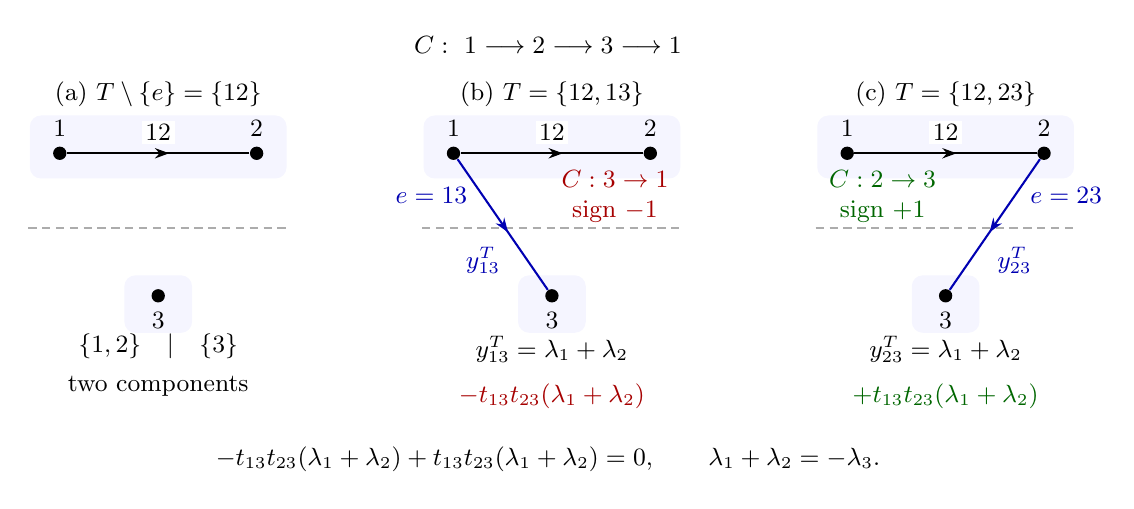
\begin{tikzpicture}[font=\small,
  tree cancellation vertex/.style={circle,fill=black,inner sep=1.7pt},
  tree cancellation edge/.style={line width=.75pt,postaction={decorate},
    decoration={markings,mark=at position .56 with
      {\arrow{Stealth[length=1.8mm,width=1.3mm]}}}},
  tree cancellation label/.style={fill=white,inner sep=1.3pt},
  tree cancellation cut/.style={gray!65,dash pattern=on 3pt off 2pt,line width=.45pt}]
  \node at (6.2,2.72) {$C:\ 1\longrightarrow2\longrightarrow3\longrightarrow1$};
  \begin{scope}
    \node at (1.25,2.10) {(a) $T\setminus\{e\}=\{12\}$};
    \fill[blue!4,rounded corners=4pt] (-.38,1.03) rectangle (2.88,1.83);
    \fill[blue!4,rounded corners=4pt] (.82,-.93) rectangle (1.68,-.20);
    \node[tree cancellation vertex,label=above:$1$] (a1) at (0,1.35) {};
    \node[tree cancellation vertex,label=above:$2$] (a2) at (2.5,1.35) {};
    \node[tree cancellation vertex,label=below:$3$] (a3) at (1.25,-.46) {};
    \draw[tree cancellation edge] (a1)--node[tree cancellation label,above=3pt]{$12$}(a2);
    \draw[tree cancellation cut] (-.40,.40)--(2.90,.40);
    \node[align=center] at (1.25,-1.34)
      {$\{1,2\}\quad\vert\quad\{3\}$\\[3pt]two components};
  \end{scope}
  \begin{scope}[xshift=5.0cm]
    \node at (1.25,2.10) {(b) $T=\{12,13\}$};
    \fill[blue!4,rounded corners=4pt] (-.38,1.03) rectangle (2.88,1.83);
    \fill[blue!4,rounded corners=4pt] (.82,-.93) rectangle (1.68,-.20);
    \node[tree cancellation vertex,label=above:$1$] (b1) at (0,1.35) {};
    \node[tree cancellation vertex,label=above:$2$] (b2) at (2.5,1.35) {};
    \node[tree cancellation vertex,label=below:$3$] (b3) at (1.25,-.46) {};
    \draw[tree cancellation cut] (-.40,.40)--(2.90,.40);
    \draw[tree cancellation edge] (b1)--node[tree cancellation label,above=3pt]{$12$}(b2);
    \draw[tree cancellation edge,blue!70!black] (b1)--
      node[tree cancellation label,pos=.28,left=4pt]{$e=13$}
      node[tree cancellation label,pos=.6,anchor=north east,shift={(-145.4:3pt)}]{$y_{13}^{T}$}(b3);
    \node[align=center,text=red!65!black] at (2.05,.80) {$C:3\to1$\\sign $-1$};
    \node at (1.25,-1.14) {$y_{13}^{T}=\lambda_1+\lambda_2$};
    \node[text=red!65!black] at (1.25,-1.74) {$-t_{13}t_{23}(\lambda_1+\lambda_2)$};
  \end{scope}
  \begin{scope}[xshift=10.0cm]
    \node at (1.25,2.10) {(c) $T=\{12,23\}$};
    \fill[blue!4,rounded corners=4pt] (-.38,1.03) rectangle (2.88,1.83);
    \fill[blue!4,rounded corners=4pt] (.82,-.93) rectangle (1.68,-.20);
    \node[tree cancellation vertex,label=above:$1$] (c1) at (0,1.35) {};
    \node[tree cancellation vertex,label=above:$2$] (c2) at (2.5,1.35) {};
    \node[tree cancellation vertex,label=below:$3$] (c3) at (1.25,-.46) {};
    \draw[tree cancellation cut] (-.40,.40)--(2.90,.40);
    \draw[tree cancellation edge] (c1)--node[tree cancellation label,above=3pt]{$12$}(c2);
    \draw[tree cancellation edge,blue!70!black] (c2)--
      node[tree cancellation label,pos=.28,right=4pt]{$e=23$}
      node[tree cancellation label,pos=.6,anchor=north west,shift={(-34.6:3pt)}]{$y_{23}^{T}$}(c3);
    \node[align=center,text=green!40!black] at (.45,.80) {$C:2\to3$\\sign $+1$};
    \node at (1.25,-1.14) {$y_{23}^{T}=\lambda_1+\lambda_2$};
    \node[text=green!40!black] at (1.25,-1.74) {$+t_{13}t_{23}(\lambda_1+\lambda_2)$};
  \end{scope}
  \node at (6.2,-2.54)
    {$-t_{13}t_{23}(\lambda_1+\lambda_2)
       +t_{13}t_{23}(\lambda_1+\lambda_2)=0,
       \qquad \lambda_1+\lambda_2=-\lambda_3.$};
\end{tikzpicture}%
}


% Native resistor diagrams. Requires TikZ, arrows.meta, decorations.markings.
\tikzset{
  spider circuit vertex/.style={circle,fill=black,inner sep=1.65pt},
  spider circuit insertion/.style={rectangle,draw,fill=white,inner sep=2.3pt},
  spider circuit wire/.style={line width=.65pt,postaction={decorate},
    decoration={markings,mark=at position #1 with
      {\arrow{Stealth[length=1.8mm,width=1.3mm]}}}},
  spider circuit wire/.default=.86,
  spider circuit resistor/.style={B wavy resistor,line width=.65pt},
  spider circuit source/.style={-{Stealth[length=1.8mm,width=1.3mm]},line width=.6pt},
  spider circuit step/.style={-{Stealth[length=2mm,width=1.5mm]},line width=.7pt},
  spider circuit label/.style={fill=white,inner sep=1.5pt}
}

\newcommand{\BSpiderArmStepCircuit}{%
\begin{tikzpicture}[font=\small]
  \node at (1.5,3.43) {(a) Before eliminating $v_{i,j}$};
  \node at (7.25,3.43) {(b) Series replacement};
  \node at (12.3,3.43) {(c) Parallel merge};
  \node[spider circuit vertex,label=below left:$v_{i,j}$] (a1) at (.2,1.78) {};
  \node[spider circuit vertex,label=above right:$v_{i,j+1}$] (a2) at (2.8,1.78) {};
  \node[spider circuit insertion,label=below right:$B$] (ab) at (1.5,-.55) {};
  \draw[spider circuit wire,blue!65!black] (a1)--
    node[spider circuit resistor]{}
    node[spider circuit label,above=4pt]{$t_{v_{i,j}v_{i,j+1}}$}(a2);
  \draw[spider circuit wire,blue!65!black] (a1)--
    node[spider circuit resistor]{}
    node[spider circuit label,anchor=north east,shift={(-150.8:4pt)}]{$t_{v_{i,j}B}^{\mathrm{red}}$}(ab);
  \draw[spider circuit wire] (a2)--node[spider circuit resistor]{}
    node[spider circuit label,anchor=north west,shift={(-29.2:4pt)}]{$t_{v_{i,j+1}B}$}(ab);
  \draw[spider circuit source] (.2,2.45)--(a1);
  \node[above] at (.2,2.45) {$\lambda_{v_{i,j}}^{\mathrm{red}}$};
  \draw[spider circuit source] (1.5,-1.19)--(ab);
  \node[left] at (1.40,-1.04) {$\lambda_B^{\mathrm{red}}$};
  \draw[spider circuit wire] (a2)--(3.6,1.78);

  \draw[spider circuit step] (3.8,.29)--(4.5,.29);
  \node[font=\footnotesize,align=center] at (4.15,-.21) {eliminate\\$v_{i,j}$};
  \node[spider circuit vertex,label=above right:$v_{i,j+1}$] (b2) at (7.25,1.78) {};
  \node[spider circuit insertion,label=below right:$B$] (bb) at (7.25,-.55) {};
  \coordinate (blt) at (6.35,1.24);
  \coordinate (blb) at (6.35,-.01);
  \coordinate (brt) at (8.15,1.24);
  \coordinate (brb) at (8.15,-.01);
  \draw[blue!65!black,line width=.65pt] (b2)--(blt);
  \draw[spider circuit wire=.6,blue!65!black] (blb)--(bb);
  \draw[blue!65!black,line width=.65pt] (blt)--node[spider circuit resistor]{}
    node[spider circuit label,left=4pt]{$\displaystyle\frac{t_{v_{i,j+1}B}^{\mathrm{red}}}{r_{i,2j}}$}(blb);
  \draw[line width=.65pt] (b2)--(brt);
  \draw[spider circuit wire=.6] (brb)--(bb);
  \draw[line width=.65pt] (brt)--node[spider circuit resistor]{}
    node[spider circuit label,right=4pt]{$t_{v_{i,j+1}B}$}(brb);
  \draw[spider circuit source] (7.25,2.45)--(b2);
  \node[above] at (7.25,2.45) {$\lambda_{v_{i,j+1}}^{\mathrm{red}}$};
  \draw[spider circuit source] (7.25,-1.19)--(bb);
  \node[left] at (7.15,-1.04) {$\lambda_B^{\mathrm{red}}$};
  \draw[spider circuit wire] (b2)--(9.0,1.78);

  \draw[spider circuit step] (9.7,.29)--(10.42,.29);
  \node[font=\footnotesize] at (10.06,-.21) {merge};
  \node[spider circuit vertex,label=above right:$v_{i,j+1}$] (c2) at (12.3,1.78) {};
  \node[spider circuit insertion,label=below right:$B$] (cb) at (12.3,-.55) {};
  \draw[spider circuit wire] (c2)--node[spider circuit resistor]{}
    node[spider circuit label,right=4pt]{$t_{v_{i,j+1}B}^{\mathrm{red}}$}
    node[spider circuit label,left=4pt]{$y_{v_{i,j+1}B}^{\mathrm{red}}$}(cb);
  \draw[spider circuit source] (12.3,2.45)--(c2);
  \node[above] at (12.3,2.45) {$\lambda_{v_{i,j+1}}^{\mathrm{red}}$};
  \draw[spider circuit source] (12.3,-1.19)--(cb);
  \node[left] at (12.2,-1.04) {$\lambda_B^{\mathrm{red}}$};
  \draw[spider circuit wire] (c2)--(13.2,1.78);

  \node at (6.4,-1.75) {$\displaystyle
    \lambda_{v_{i,j+1}}^{\mathrm{red}}=r_{i,2j-1}\lambda_{v_{i,j}}^{\mathrm{red}},
    \qquad \lambda_B^{\mathrm{red}}\longmapsto
    \lambda_B^{\mathrm{red}}+(1-r_{i,2j-1})\lambda_{v_{i,j}}^{\mathrm{red}}.$};
  \node at (6.4,-2.54) {$\displaystyle
    t_{v_{i,j}v_{i,j+1}}+t_{v_{i,j}B}^{\mathrm{red}}
      =\frac{t_{v_{i,j+1}B}^{\mathrm{red}}}{r_{i,2j}},
    \qquad t_{v_{i,j+1}B}
      =\frac{t_{v_{i,j+1}B}^{\mathrm{red}}}{1-r_{i,2j}}.$};
  \node[align=left] at (6.4,-4.08) {$\displaystyle
    y_{v_{i,j}v_{i,j+1}}=
      r_{i,2j-1}\lambda_{v_{i,j}}^{\mathrm{red}}
      -\textcolor{blue!65!black}{r_{i,2j}y_{v_{i,j+1}B}^{\mathrm{red}}}$\\[7pt]
    $\displaystyle y_{v_{i,j}B}^{\mathrm{red}}=
      (1-r_{i,2j-1})\lambda_{v_{i,j}}^{\mathrm{red}}
      +\textcolor{blue!65!black}{r_{i,2j}y_{v_{i,j+1}B}^{\mathrm{red}}}$\\[7pt]
    $\displaystyle y_{v_{i,j+1}B}=
      (1-r_{i,2j})y_{v_{i,j+1}B}^{\mathrm{red}}$};
\end{tikzpicture}%
}

% Native TikZ, with no external assets or circuit package.
% Requires amsmath, amssymb, tikz, arrows.meta and decorations.markings.
\tikzset{
  BFC wire/.style={line width=.6pt,draw=black!85,postaction={decorate},
    decoration={markings,mark=at position #1 with {\arrow[blue!65!black]{Stealth[length=1.6mm,width=1.1mm]}}}},
  BFC wire/.default=.78,
  BFC resistor/.style={B wavy resistor,draw=black!85,line width=.6pt},
  BFC vertex/.style={circle,fill=black,inner sep=1.6pt},
  BFC insertion/.style={rectangle,draw,fill=white,inner sep=2.3pt},
  BFC source/.style={-{Stealth[length=1.6mm,width=1.1mm]},line width=.55pt},
  BFC label/.style={fill=white,inner sep=1.2pt},
  BFC current/.style={BFC label,text=blue!65!black},
  BFC step/.style={-{Stealth[length=1.8mm,width=1.3mm]},line width=.65pt}
}
\newcommand{\BFanCurrentInductionCircuit}{%
\begin{tikzpicture}[font=\fontsize{9.2}{10.8}\selectfont]
  % The base case: the last triangle.
  \begin{scope}[yshift=.12cm]
  \node[anchor=west] at (-.1,6.82) {(a) Start from the final triangle};
  \node[BFC vertex,label=below left:$n$] (tn) at (0,5.40) {};
  \node[BFC vertex,label=below right:$n+1$] (tnp) at (4.4,5.40) {};
  \node[BFC insertion,label=right:$n+2$] (to) at (2.2,3.76) {};
  \draw[BFC source] (0,6.07)--(tn);
  \node[above] at (0,6.07) {$\lambda_n^{\mathrm{red}}$};
  \draw[BFC source] (4.4,6.07)--(tnp);
  \node[above] at (4.4,6.07) {$\lambda_{n+1}$};
  \draw[BFC wire] (tn)--node[pos=.48,BFC resistor]{}
    node[pos=.48,BFC label,above=3pt]{$1-r_{2n-1}-r_{2n}$}
    node[pos=.48,BFC current,below=3pt]{$y_{n,n+1}$}(tnp);
  \draw[BFC wire] (tn)--node[pos=.48,BFC resistor]{}
    node[pos=.48,BFC label,anchor=north east,shift={(-126.7:3pt)},align=right]
      {$r_{2n-1}$\\[2pt]\textcolor{blue!65!black}{$y_{n,n+2}^{\mathrm{red}}$}}(to);
  \draw[BFC wire] (tnp)--node[pos=.48,BFC resistor]{}
    node[pos=.48,BFC label,anchor=north west,shift={(-53.3:3pt)},align=left]
      {$r_{2n}$\\\textcolor{blue!65!black}{$y_{n+1,n+2}$}}(to);
  \draw[BFC source] (2.2,3.35)--(to);
  \node[below] at (2.2,3.35) {$\lambda_{n+2}^{\mathrm{red}}$};
  \node[anchor=west,align=left] at (6.35,5.1) {$\begin{aligned}
    y_{n,n+2}^{\mathrm{red}}&=\lambda_n^{\mathrm{red}}-y_{n,n+1},\\
    y_{n+1,n+2}&=\lambda_{n+1}+y_{n,n+1},\\[3pt]
    0={}&(1-r_{2n-1}-r_{2n})y_{n,n+1}\\
      &+r_{2n}(\lambda_{n+1}+y_{n,n+1})\\
      &-r_{2n-1}(\lambda_n^{\mathrm{red}}-y_{n,n+1}),\\[3pt]
    \textcolor{blue!65!black}{y_{n,n+1}}
      &\textcolor{blue!65!black}{=r_{2n-1}\lambda_n^{\mathrm{red}}-r_{2n}\lambda_{n+1}.}
  \end{aligned}$};
  \end{scope}
  % One backward step at a general path vertex.
  \node at (1.20,2.62) {(b) Reduced spoke};
  \node at (6.55,2.62) {(c) Split the parallel currents};
  \node at (12.32,2.62) {(d) Restore vertex $i$};
  \node[BFC vertex,label=above left:$i+1$] (b) at (1.2,1.12) {};
  \node[BFC insertion,label=right:$n+2$] (bo) at (1.2,-.69) {};
  \draw[BFC source] (1.2,1.84)--(b);
  \node[above] at (1.2,1.84) {$\lambda_{i+1}^{\mathrm{red}}$};
  \draw[BFC wire] (b)--node[pos=.42,BFC resistor]{}
    node[pos=.42,BFC label,right=3pt]{$t_{i+1,n+2}^{\mathrm{red}}$}
    node[pos=.42,BFC current,left=3pt]{$y_{i+1,n+2}^{\mathrm{red}}$}(bo);
  \draw[BFC wire] (b)--node[BFC current,above=3pt]{$y_{i+1,i+2}$}(2.95,1.12);
  \draw[BFC step] (3.03,-1.04)--(3.88,-1.04);
  \node[below,font=\fontsize{8.2}{9.6}\selectfont] at (3.455,-1.04) {undo merge};
  \node[BFC vertex,label=above left:$i+1$] (p) at (6.55,1.12) {};
  \node[BFC insertion,label=below:$n+2$] (po) at (6.55,-.69) {};
  \draw[BFC source] (6.55,1.84)--(p);
  \node[above] at (6.55,1.84) {$\lambda_{i+1}^{\mathrm{red}}$};
  \draw[BFC wire=.91] (p) -- ++(-.62,-.3) -- node[pos=.42,BFC resistor]{}
    node[pos=.42,BFC label,left=5pt]{$\dfrac{t_{i+1,n+2}^{\mathrm{red}}}{1-r_{2i}}$}
    node[pos=.95,BFC current,left=4pt,yshift=-6pt]{$(1-r_{2i})y_{i+1,n+2}^{\mathrm{red}}$} ($(po)+(-.62,.3)$) -- (po);
  \draw[BFC wire=.91] (p) -- ++(.62,-.3) -- node[pos=.42,BFC resistor]{}
    node[pos=.42,BFC label,right=5pt]{$\dfrac{t_{i+1,n+2}^{\mathrm{red}}}{r_{2i}}$}
    node[pos=.95,BFC current,right=4pt,yshift=-6pt]{$r_{2i}y_{i+1,n+2}^{\mathrm{red}}$} ($(po)+(.62,.3)$) -- (po);
  \node[font=\fontsize{8.1}{9.3}\selectfont] at (4.85,.9) {new branch};
  \node[font=\fontsize{8.1}{9.3}\selectfont] at (8.38,.9) {original spoke};
  \draw[BFC wire] (p)--node[BFC current,above=3pt]{$y_{i+1,i+2}$}(8.32,1.12);
  \draw[BFC step] (9.1,-1.04)--(9.95,-1.04);
  \node[below,font=\fontsize{8.2}{9.6}\selectfont] at (9.525,-1.04) {undo series};
  \node[BFC vertex,label=below left:$i$] (di) at (10.18,1.12) {};
  \node[BFC vertex,label=above left:$i+1$] (dj) at (13.10,1.12) {};
  \node[BFC insertion,label=right:$n+2$] (dO) at (13.10,-.69) {};
  \draw[BFC source] (10.18,1.84)--(di);
  \node[above] at (10.18,1.84) {$\lambda_i^{\mathrm{red}}$};
  \draw[BFC source] (13.10,1.84)--(dj);
  \node[above] at (13.10,1.84) {$\lambda_{i+1}$};
  \draw[BFC wire] (di)--node[pos=.48,BFC resistor]{}
    node[pos=.48,BFC label,above=3pt]{$t_{i,i+1}$}
    node[pos=.48,BFC current,below=3pt]{$y_{i,i+1}$}(dj);
  \draw[BFC wire] (di)--node[pos=.43,BFC resistor]{}
    node[pos=.43,BFC label,anchor=north east,shift={(-121.8:3pt)},align=right]
      {$t_{i,n+2}^{\mathrm{red}}$\\[2pt]\textcolor{blue!65!black}{$y_{i,n+2}^{\mathrm{red}}$}}(dO);
  \draw[BFC wire] (dj)--node[pos=.42,BFC resistor]{}
    node[pos=.42,BFC label,right=3pt,align=left]
      {$t_{i+1,n+2}$\\\textcolor{blue!65!black}{$y_{i+1,n+2}$}}(dO);
  \draw[BFC wire] (dj)--node[BFC current,above=3pt]{$y_{i+1,i+2}$}(14.86,1.12);
  \node at (7.03,-1.94) {$\displaystyle
    \lambda_{i+1}^{\mathrm{red}}=\lambda_{i+1}+r_{2i-1}\lambda_i^{\mathrm{red}},
    \qquad \textcolor{blue!65!black}{y_{i+1,n+2}^{\mathrm{red}}
      =\lambda_{i+1}^{\mathrm{red}}-y_{i+1,i+2}}.$};
  \node at (7.03,-2.53) {$\displaystyle
    \textcolor{blue!65!black}{
      y_{i,i+1}=r_{2i-1}\lambda_i^{\mathrm{red}}
        -(1-r_{2i})y_{i+1,n+2}^{\mathrm{red}},
      \qquad y_{i+1,n+2}=r_{2i}y_{i+1,n+2}^{\mathrm{red}}}.$};
\end{tikzpicture}%
}


% Native resistor diagrams; TikZ libraries arrows.meta, decorations.markings.
\tikzset{
  spider jac vertex/.style={circle,fill=black,inner sep=1.7pt},
  spider jac insertion/.style={rectangle,draw,fill=white,inner sep=2.2pt},
  spider jac edge/.style={line width=.65pt,postaction={decorate},
    decoration={markings,mark=at position #1 with
      {\arrow{Stealth[length=1.65mm,width=1.2mm]}}}},
  spider jac edge/.default=.76,
  spider jac resistor/.style={B wavy resistor,line width=.65pt},
  spider jac omitted/.style={gray!35,dash pattern=on 2.5pt off 1.8pt},
  spider jac label/.style={fill=white,inner sep=1.1pt},
  spider jac step/.style={-{Stealth[length=1.8mm,width=1.3mm]},line width=.7pt}
}

\newcommand{\BSpiderJacobianCoordinatesCircuit}{%
\begin{tikzpicture}[font=\fontsize{9.5}{11.4}\selectfont]
  \node at (1.7,2.2) {Three local resistances};
  \node[spider jac vertex,label=above left:$v_{i,j}$] (u) at (.2,1.36) {};
  \node[spider jac vertex,label=above right:$v_{i,j+1}$] (v) at (3.2,1.36) {};
  \node[spider jac insertion,label=below:$B$] (b) at (1.7,-.82) {};
  \draw[spider jac edge] (u)--node[spider jac resistor]{}
    node[spider jac label,above=4pt]{$t_{v_{i,j}v_{i,j+1}}$}(v);
  \draw[spider jac edge] (u)--node[spider jac resistor]{}
    node[spider jac label,anchor=north east,shift={(-145.5:4pt)}]{$t_{v_{i,j}B}^{\mathrm{red}}$}(b);
  \draw[spider jac edge] (v)--node[spider jac resistor]{}
    node[spider jac label,anchor=north west,shift={(-34.5:4pt)}]{$t_{v_{i,j+1}B}$}(b);
  \draw[spider jac step] (4.47,.25)--(5.47,.25);
  \node[align=center] at (4.97,-.28) {eliminate\\$v_{i,j}$};
  \node at (7.2,2.2) {Effective spoke};
  \node[spider jac vertex,label=above:$v_{i,j+1}$] (rv) at (7.2,1.36) {};
  \node[spider jac insertion,label=below:$B$] (rb) at (7.2,-.82) {};
  \draw[spider jac edge=.82] (rv)--node[spider jac resistor]{}
    node[spider jac label,right=4pt]{$t_{v_{i,j+1}B}^{\mathrm{red}}$}(rb);
  \node[align=left,anchor=west] at (9.3,.28) {$\displaystyle
    t_{v_{i,j}v_{i,j+1}}=
    \frac{1-r_{i,2j-1}}{r_{i,2j}}\,t_{v_{i,j+1}B}^{\mathrm{red}}$\\[10pt]
    $\displaystyle t_{v_{i,j}B}^{\mathrm{red}}=
    \frac{r_{i,2j-1}}{r_{i,2j}}\,t_{v_{i,j+1}B}^{\mathrm{red}}$\\[10pt]
    $\displaystyle t_{v_{i,j+1}B}=
    \frac1{1-r_{i,2j}}\,t_{v_{i,j+1}B}^{\mathrm{red}}$};
\end{tikzpicture}%
}

% Six arguments: x, y, path style, old-spoke style, next-spoke style, weight.
% These are drawing arguments, not additional notation in the figure.
\newcommand{\BSpiderJacobianLiftTriangle}[6]{%
\begin{scope}[xshift=#1cm,yshift=#2cm]
  \node[spider jac vertex,label=above left:$v_{i,j}$] (u) at (-1.1,1.12) {};
  \node[spider jac vertex,label=above right:$v_{i,j+1}$] (v) at (1.1,1.12) {};
  \node[spider jac insertion,label=below:$B$] (b) at (0,-.58) {};
  \draw[spider jac edge,#3] (u)--node[spider jac resistor]{}(v);
  \draw[spider jac edge,#4] (u)--node[spider jac resistor]{}(b);
  \draw[spider jac edge,#5] (v)--node[spider jac resistor]{}(b);
  \node at (0,-1.27) {$#6$};
\end{scope}%
}

\newcommand{\BSpiderJacobianTreeLiftsCircuit}{%
\begin{tikzpicture}[font=\fontsize{9.5}{11.4}\selectfont,spider jac edge/.default=.88]
  \node[anchor=west] at (-.1,3.04) {Solid: in the tree. Pale: omitted. Below each lift: product of omitted resistances.};
  \node[anchor=west] at (-.1,2.40) {(a) The reduced tree contains the effective spoke.};
  \node[spider jac vertex,label=above:$v_{i,j+1}$] (uv) at (.65,1.12) {};
  \node[spider jac insertion,label=below:$B$] (ub) at (.65,-.58) {};
  \draw[spider jac edge] (uv)--node[spider jac resistor]{}
    node[spider jac label,right=4pt]{$t_{v_{i,j+1}B}^{\mathrm{red}}$}(ub);
  \node[align=center] at (.65,-1.27) {reduced weight $1$};
  \draw[spider jac step] (2.05,.3)--(2.77,.3);
  \node[font=\fontsize{8.5}{10}\selectfont,align=center] at (2.41,-.14) {three\\lifts};
  \BSpiderJacobianLiftTriangle{4.2}{0}{spider jac omitted}{black}{black}{t_{v_{i,j}v_{i,j+1}}}
  \BSpiderJacobianLiftTriangle{8.4}{0}{black}{spider jac omitted}{black}{t_{v_{i,j}B}^{\mathrm{red}}}
  \BSpiderJacobianLiftTriangle{12.6}{0}{black}{black}{spider jac omitted}{t_{v_{i,j+1}B}}
  \node at (6.45,-2.12) {$\displaystyle
    t_{v_{i,j}v_{i,j+1}}+t_{v_{i,j}B}^{\mathrm{red}}+t_{v_{i,j+1}B}
    =\frac{t_{v_{i,j+1}B}^{\mathrm{red}}}{r_{i,2j}(1-r_{i,2j})}.$};

  \node[anchor=west] at (-.1,-3.35) {(b) The reduced tree omits the effective spoke.};
  \begin{scope}[yshift=-5.32cm]
    \node[spider jac vertex,label=above:$v_{i,j+1}$] (ov) at (.65,1.12) {};
    \node[spider jac insertion,label=below:$B$] (ob) at (.65,-.58) {};
    \draw[spider jac edge,spider jac omitted] (ov)--node[spider jac resistor]{}(ob);
    \node[align=center] at (.65,-1.62) {reduced weight\\[3pt]$t_{v_{i,j+1}B}^{\mathrm{red}}$};
    \draw[spider jac step] (2.05,.3)--(2.77,.3);
    \node[font=\fontsize{8.5}{10}\selectfont,align=center] at (2.41,-.14) {two\\lifts};
    \BSpiderJacobianLiftTriangle{5.2}{0}{black}{spider jac omitted}{spider jac omitted}{t_{v_{i,j}B}^{\mathrm{red}}t_{v_{i,j+1}B}}
    \BSpiderJacobianLiftTriangle{10.2}{0}{spider jac omitted}{black}{spider jac omitted}{t_{v_{i,j}v_{i,j+1}}t_{v_{i,j+1}B}}
  \end{scope}
  \node at (6.45,-7.84) {$\displaystyle
    t_{v_{i,j+1}B}\bigl(t_{v_{i,j}v_{i,j+1}}+t_{v_{i,j}B}^{\mathrm{red}}\bigr)
    =\frac{t_{v_{i,j+1}B}^{\mathrm{red}}}{r_{i,2j}(1-r_{i,2j})}
      \,t_{v_{i,j+1}B}^{\mathrm{red}}.$};
  \node[anchor=west] at (-.1,-8.74) {Only the local edges are shown; the rest of the tree is fixed.};
\end{tikzpicture}%
}


% Native TikZ. Dependencies: amsmath, amssymb, arrows.meta, decorations.markings.
% Resistor values are black, oriented branch currents blue, injected sources black.
\tikzset{
  BBook wire/.style={line width=.6pt,draw=black!85,postaction={decorate},
    decoration={markings,mark=at position #1 with {\arrow[blue!65!black]{Stealth[length=1.6mm,width=1.1mm]}}}},
  BBook wire/.default=.90,
  BBook resistor/.style={B wavy resistor,draw=black!85,line width=.6pt},
  BBook vertex/.style={circle,fill=black,inner sep=1.6pt},
  BBook insertion/.style={rectangle,draw,fill=white,inner sep=2.3pt},
  BBook source/.style={-{Stealth[length=1.6mm,width=1.1mm]},line width=.55pt},
  BBook label/.style={fill=white,inner sep=1.2pt},
  BBook current/.style={BBook label,text=blue!65!black},
  BBook step/.style={-{Stealth[length=1.8mm,width=1.3mm]},line width=.65pt}
}
\newcommand{\BBookCurrentReductionCircuit}{%
\begin{tikzpicture}[x=.96cm,font=\fontsize{9.2}{10.8}\selectfont]
  \node at (2.60,5.05) {(a) Leaves $1,\ldots,i,\ldots,n$};
  \node at (9.00,5.05) {(b) $n+1$ parallel branches};
  \node at (13.85,5.05) {(c) Unit resistor};
  % Representative leaves: omitted leaves obey the same local reduction.
  \node[BBook vertex,label=below left:$n+1$] (aA) at (0,0) {};
  \node[BBook insertion,label=below right:$n+2$] (aB) at (5.2,0) {};
  \node[BBook vertex,label=right:$1$] (a1) at (2.6,3.7) {};
  \node[BBook vertex,label=above right:$i$] (ai) at (2.6,2.15) {};
  \node[BBook vertex,label=left:$n$] (an) at (2.6,-1.46) {};
  \draw[BBook source] (0,-.63)--(aA);
  \node[below] at (0,-.63) {$\lambda_{n+1}$};
  \draw[BBook source] (5.2,-.63)--(aB);
  \node[below] at (5.2,-.63) {$\lambda_{n+2}$};
  \draw[BBook source] (2.6,4.32)--(a1);
  \node[above] at (2.6,4.32) {$\lambda_1$};
  \draw[BBook source] (2.6,2.77)--(ai);
  \node[above] at (2.6,2.77) {$\lambda_i$};
  \draw[BBook source] (2.6,-2.09)--(an);
  \node[below] at (2.6,-2.09) {$\lambda_n$};
  \draw[BBook wire] (a1)--node[BBook resistor]{}(aA);
  \draw[BBook wire] (a1)--node[BBook resistor]{}(aB);
  \draw[BBook wire] (ai)--node[BBook resistor]{}
    node[BBook label,anchor=north west,shift={(-49.3:3pt)},align=left]
      {$t_{i,n+1}$\\\textcolor{blue!65!black}{$y_{i,n+1}$}}(aA);
  \draw[BBook wire] (ai)--node[BBook resistor]{}
    node[BBook label,anchor=north east,shift={(-130.7:3pt)},align=right]
      {$t_{i,n+2}$\\\textcolor{blue!65!black}{$y_{i,n+2}$}}(aB);
  \draw[BBook wire] (an)--node[BBook resistor]{}(aA);
  \draw[BBook wire] (an)--node[BBook resistor]{}(aB);
  \draw[BBook wire] (aA)--node[BBook resistor]{}
    node[BBook label,below=4pt]{$t_{n+1,n+2}$}(aB);
  \node at (3.50,1.91) {$\vdots$};
  \node at (2.95,-.88) {$\vdots$};
  \draw[BBook step] (5.65,-1.22)--(6.73,-1.22);
  \node[below,align=center,font=\fontsize{8.4}{9.8}\selectfont] at (6.19,-1.22)
    {eliminate\\all leaves};
  % The original common edge plus one series branch from each leaf.
  \begin{scope}[yshift=.5cm]
  \node[BBook vertex,label=above left:$n+1$] (bA) at (9.00,2.46) {};
  \node[BBook insertion,label=below right:$n+2$] (bB) at (9.00,-1.20) {};
  \draw[BBook source] (9.00,3.11)--(bA);
  \node[above] at (9.00,3.11) {$\lambda_{n+1}^{\mathrm{red}}$};
  \draw[BBook source] (9.00,-1.96)--(bB);
  \node[below] at (9.00,-1.96) {$\lambda_{n+2}^{\mathrm{red}}$};
  \draw[BBook wire] (bA) -- ++(-1.3,-.4) -- node[pos=.5,BBook resistor]{}
    node[pos=.5,BBook label,left=4pt]{$\dfrac1{1-\sum_{j=1}^n r_{2j}}$} ($(bB)+(-1.3,.4)$) -- (bB);
  \draw[BBook wire=.935] (bA) -- ++(-.45,-.4) -- node[pos=.5,BBook resistor]{} ($(bB)+(-.45,.4)$) -- (bB);
  \draw[BBook wire=.935] (bA) -- ++(.45,-.4) -- node[pos=.5,BBook resistor]{} ($(bB)+(.45,.4)$) -- (bB);
  \draw[BBook wire] (bA) -- ++(1.3,-.4) -- node[pos=.5,BBook resistor]{}
    node[pos=.5,BBook label,right=4pt]{$1/r_{2i}$}
    node[pos=.85,BBook current,right=4pt]{$r_{2i}y_{n+1,n+2}^{\mathrm{red}}$} ($(bB)+(1.3,.4)$) -- (bB);
  \node at (9.00,.63) {$\cdots$};
  \node[BBook label,font=\fontsize{8.3}{9.6}\selectfont,anchor=east] at (7.58,-.25) {original edge};
  \draw[BBook step] (11.40,-1.72)--(12.41,-1.72);
  \node[below,font=\fontsize{8.4}{9.8}\selectfont] at (11.90,-1.72) {merge};
  % Conductances sum to one, so the common scale gives a unit resistance.
  \node[BBook vertex,label=above left:$n+1$] (cA) at (13.85,2.46) {};
  \node[BBook insertion,label=right:$n+2$] (cB) at (13.85,-1.20) {};
  \draw[BBook source] (13.85,3.11)--(cA);
  \node[above] at (13.85,3.11) {$\lambda_{n+1}^{\mathrm{red}}$};
  \draw[BBook source] (13.85,-1.96)--(cB);
  \node[below] at (13.85,-1.96) {$\lambda_{n+2}^{\mathrm{red}}$};
  \draw[BBook wire] (cA)--node[pos=.43,BBook resistor]{}
    node[pos=.43,BBook label,right=4pt]{$1$}
    node[pos=.43,BBook current,left=4pt]{$y_{n+1,n+2}^{\mathrm{red}}$}(cB);
  \end{scope}
  % The displayed currents are the ones differentiated in the book Jacobian.
  \node at (7.15,-3.17) {$\displaystyle
    \lambda_{n+1}^{\mathrm{red}}
      =\lambda_{n+1}+\sum_{i=1}^n r_{2i-1}\lambda_i
      =\textcolor{blue!65!black}{y_{n+1,n+2}^{\mathrm{red}}},
    \qquad t_{n+1,n+2}^{\mathrm{red}}=1.$};
  \node at (7.15,-4.12) {$\displaystyle
    \lambda_{n+2}^{\mathrm{red}}
      =\lambda_{n+2}+\sum_{i=1}^n(1-r_{2i-1})\lambda_i
      =-\textcolor{blue!65!black}{y_{n+1,n+2}^{\mathrm{red}}}.$};
  \node at (7.15,-5.04) {$\displaystyle
    t_{i,n+1}=\frac{1-r_{2i-1}}{r_{2i}},\qquad
    t_{i,n+2}=\frac{r_{2i-1}}{r_{2i}},\qquad
    t_{i,n+1}+t_{i,n+2}=\frac1{r_{2i}}.$};
  \node at (7.15,-5.89) {$\displaystyle\textcolor{blue!65!black}{
    y_{i,n+1}=r_{2i-1}\lambda_i-r_{2i}y_{n+1,n+2}^{\mathrm{red}},\qquad
    y_{i,n+2}=(1-r_{2i-1})\lambda_i+r_{2i}y_{n+1,n+2}^{\mathrm{red}}}.$};
  \node at (7.15,-6.78) {$\displaystyle\textcolor{blue!65!black}{
    y_{n+1,n+2}=\left(1-\sum_{i=1}^n r_{2i}\right)y_{n+1,n+2}^{\mathrm{red}}},
    \qquad \frac1{t_{n+1,n+2}}+\sum_{i=1}^n r_{2i}=1.$};
\end{tikzpicture}%
}

\clearpage
\section{Graph integrals and network reductions}
\label{sec:network}

Sections~\ref{sec:B-propagators}--\ref{sec:B-kernel} review the propagators, the $\mathcal N=4$ superfield and the reduction of the bracket graphs to current integrals \cite{Costello,Wang,operatope,ChangYin,BK}; the remaining sections reduce these integrals as electrical networks.

\subsection{Pairing and propagators}
\label{sec:B-propagators}

For vertices $v,w$ of a graph of the brackets \eqref{eq:A.28}, the inverse BV pairing contracts a $\mathsf c$ field at one vertex with a $\mathsf b$ field at the other, or a $\gamma$ field with a $\beta$ field. Its fibre part is the operator

\begin{equation}\label{eq:A.20}
\begin{aligned}
\Delta_{vw}={}&
\frac{\partial_L}{\partial\mathsf b_{A,v}}
\frac{\partial_L}{\partial\mathsf c_w^A}
+
\frac{\partial_L}{\partial\mathsf c_v^A}
\frac{\partial_L}{\partial\mathsf b_{A,w}}
\\
&-
\frac{\partial_L}{\partial\beta_v^i}
\frac{\partial_L}{\partial\gamma_{i,w}}
-
\frac{\partial_L}{\partial\gamma_{i,v}}
\frac{\partial_L}{\partial\beta_w^i}.
\end{aligned}
\end{equation}

Dolbeault gauge fixing uses $Q^{\mathrm{GF}}=\bar\partial^*$ and $H=\{\bar\partial,Q^{\mathrm{GF}}\}$ \cite{Costello}. With $\omega_E^{-1}$ the distributional inverse BV pairing, define the heat kernel $K_t$ by
\begin{equation}\label{eq:propagator}
K_t=(e^{-tH}\otimes1)\omega_E^{-1},\qquad 0<\varepsilon<L.
\end{equation}

For two Euclidean spacetime points $x_1,x_2$, the heat kernel is
\begin{equation}\label{eq:C-heat-spatial}
[K_t(x_1,x_2)]_\Omega
=-\frac{e^{-|x_1-x_2|_E^2/(2t)}}{32\pi^2t^2}
 d(x_1-x_2)^{-\dot+}\wedge d(x_1-x_2)^{-\dot-}.
\end{equation}
The propagator $P_{\varepsilon,L}$ is the Schwinger-time integral
\begin{equation}\label{eq:C-heat-homotopy}
\begin{aligned}
P_{\varepsilon,L}
&=\int_\varepsilon^L(Q^{\mathrm{GF}}\otimes1)K_t\,dt,\\
(\bar\partial\otimes1+1\otimes\bar\partial)P_{\varepsilon,L}
&=-\int_\varepsilon^L\partial_tK_t\,dt
=K_\varepsilon-K_L.
\end{aligned}
\end{equation}
The free BV differential raises antiholomorphic form degree by one,
turning a degree-one propagator into a degree-two heat kernel, the
regularized delta function. These are the heat-kernel conventions of
\cite{Costello,Wang}.

Intuitively, applying the free differential $\bar\partial$ to a graph replaces one propagator by a heat kernel. Figure~\ref{fig:Q-graphs} shows this operation for the segment, triangle and two-loop fan.
\begin{figure}[H]
\centering
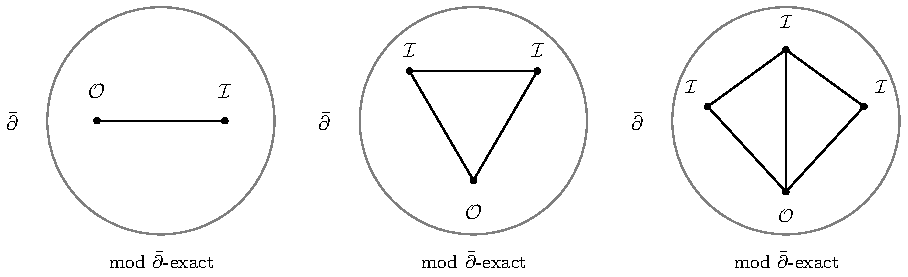
\includegraphics[width=0.98\linewidth,height=.70\textheight,keepaspectratio]{figures/feynarts/fa_Q_graphs.pdf}
\caption{The free differential $\bar\partial$ acting on the tree, one-loop and two-loop contraction graphs. The interaction vertices are labelled $\mathcal I$ and the local insertion is $\mathcal O$.}
\label{fig:Q-graphs}
\end{figure}

A holomorphic displacement $z_{v,i}$ generates derivatives of the $i$th field at vertex $v$, as needed when computing $Q(\beta\,\partial_{+\dot a}\gamma)$. Translating the field to $x_v+z_{v,i}$, differentiating in $z_{v,i}$, and setting $z_{v,i}=0$ gives its holomorphic derivatives. In a contraction between fields at $v$ and $w$, the propagator therefore has argument $x_v-x_w+z_e$, with $z_e=z_{v,i}-z_{w,j}$. For example, on the oriented edge $(1,3)$,
\begin{equation}\label{eq:input-displacement}
\left.\partial_{3,+\dot a}
[P_{\varepsilon,L;13}(x_1-x_3+z_{13})]_\Omega\right|_{z_{13}=0}
=\left.2\frac{\partial}{\partial z_{13}^{+\dot a}}
[P_{\varepsilon,L;13}(x_1-x_3+z_{13})]_\Omega\right|_{z_{13}=0}.
\end{equation}

\subsection{The \texorpdfstring{$\mathcal N=4$}{N=4} superfield}
\label{sec:N4-superfield}

Most of our examples use $\mathcal N=4$ Yang--Mills theory, the gauge theory of the best-studied example of the AdS/CFT correspondence. Its three adjoint chiral multiplets have fields $(\gamma^I)_A,(\beta_I)^A$, $I=1,2,3$, and the adjoint generators are $(t_A^{\mathrm{adj}})^B{}_C=iC^B{}_{AC}$. The holomorphic twist uses $Q_-^4$. The supercharges $Q_+^I$, $I=1,2,3$, act as translations in the odd coordinates $\theta_I$, with $\int d^3\theta\,\theta_1\theta_2\theta_3=1$ and $\theta_I\bar\partial=-\bar\partial\theta_I$. The fields of the holomorphic twist combine into one superfield \cite{ChangYin}, \cite[Equation (3.52)]{BK}, up to rescaling of the components,
\begin{equation}\label{eq:A.13}
C^A(\theta)=ig\,\mathsf c^A+\theta_I\delta^{AB}(\gamma^I)_B-\frac12\varepsilon^{IJK}\theta_I\theta_J(\beta_K)^A+\frac{\theta_1\theta_2\theta_3}{ig}\delta^{AB}\mathsf b_B,
\end{equation}
where $\varepsilon^{123}=\varepsilon_{123}=1$ and the component order is $\theta_IX$. The supersymmetry action is represented by left differentiation, $Q_+^IC^A(\theta)=\partial_LC^A(\theta)/\partial\theta_I$. In this convention the action and classical differential take the form

\begin{equation}\label{eq:A.15}
\begin{aligned}
S_{\mathrm{tw},E}
&=\int_{\mathbb C^2}\Omega\wedge
\left[\int d^3\theta\left(
\frac12\delta_{AB}C^A\bar\partial C^B
+\frac{i}{3!}C_{ABC}C^AC^BC^C\right)\right]_{(0,2)},\\
Q_0C^A&=\frac i2C^A{}_{BC}C^BC^C.
\end{aligned}
\end{equation}

and the superpotential is
\begin{equation}
\bar W(\gamma,0)=\frac i{3!}\varepsilon_{IJK}C_{ABC}
\delta^{AD}\delta^{BE}\delta^{CF}(\gamma^I)_D(\gamma^J)_E(\gamma^K)_F.
\end{equation}
The single cubic interaction thus contains the gauge, matter and superpotential vertices of \eqref{eq:B.10}. At a fixed spacetime point, the fibre derivative dual to $C$ is

\begin{equation}\label{eq:A.16}
\begin{aligned}
\frac{\delta}{\delta C^A(\theta)}
={}&\frac{\theta_1\theta_2\theta_3}{ig}
\frac{\partial_L}{\partial\mathsf c^A}
-\frac12\varepsilon^{IJK}\theta_J\theta_K
\frac{\partial}{\partial(\gamma^I)_A}
-\theta_I\frac{\partial_L}{\partial(\beta_I)^A}
-ig\frac{\partial}{\partial\mathsf b_A},\\
\frac{\delta C^B(\theta^{(2)})}{\delta C^A(\theta^{(1)})}
={}&\delta_A{}^B\prod_{I=1}^3
(\theta_I^{(1)}-\theta_I^{(2)}).
\end{aligned}
\end{equation}

and its contraction reproduces the component pairing:

\begin{equation}\label{eq:A.17}
\Delta_{vw}=-\delta^{DE}\int d^3\theta\,\frac{\delta}{\delta C_v^D(\theta)}\frac{\delta}{\delta C_w^E(\theta)} .
\end{equation}

For the superfield pairing, the odd factor on an oriented edge $(v,w)$ is $\delta_{vw}=\prod_{I=1}^3(\theta_I^{(v)}-\theta_I^{(w)})$.

\subsection{The kernel in Schwinger times and edge currents}
\label{sec:B-kernel}

Let $\Gamma_0=\{1,\ldots,k\}$ be the vertices and $\Gamma_1=(e_1,\ldots,e_{2n+1})$ the ordered edges of a graph. Fix the insertion at $x_k=0$ and set $\lambda_k=-\sum_{v<k}\lambda_v$. Each edge kernel has argument $x_{e(0)}-x_{e(1)}+z_e$, and $t_e>0$ is the Schwinger time of edge $e$. For $k=n+2$, the kernel is the lower-boundary sum at fixed $L>0$; summing over the heat edge turns it into an integral over the UV boundary of the Schwinger cube, as in \cite[Equations (2.12)--(2.14)]{operatope} and \cite[Lemma 2, Proposition 9]{Wang}:

\begin{equation}\label{eq:1.7}
\begin{aligned}
\mathcal I_\Gamma^{\mathrm{raw\ cut}}(\lambda;z)
={}&(-8\pi^2)^n\lim_{\varepsilon\downarrow0}
\sum_{j=1}^{2n+1}(-1)^{j-1}
\int_{(\mathbb C^2)^{k-1}}
\left(\bigwedge_{v<k}\Omega_v\right)
e^{\sum_{v<k}\lambda_{v,+\dot a}x_v^{+\dot a}}\\
&\times\left(\bigwedge_{a<j}[P_{\varepsilon,L;e_a}]_\Omega\right)
\wedge[K_{\varepsilon;e_j}]_\Omega
\wedge\left(\bigwedge_{a>j}[P_{\varepsilon,L;e_a}]_\Omega\right)\\
={}&(-8\pi^2)^n\lim_{\varepsilon\downarrow0}
\int_{(\mathbb C^2)^{k-1}}
\left(\bigwedge_{v<k}\Omega_v\right)
e^{\sum_{v<k}\lambda_{v,+\dot a}x_v^{+\dot a}}\,
\bar\partial\left(\bigwedge_{a=1}^{2n+1}[P_{\varepsilon,L;e_a}]_\Omega\right)\bigg|_{\mathrm{UV}}\\
={}&(-1)^n(-8\pi^2)^n\lim_{\varepsilon\downarrow0}
\int_{(\mathbb C^2)^{k-1}}
\left(\bigwedge_{v<k}\Omega_v\right)
e^{\sum_{v<k}\lambda_{v,+\dot a}x_v^{+\dot a}}\\
&\times\int_{\partial_{\mathrm{UV}}[\varepsilon,L]^{2n+1}}
\bigwedge_{a=1}^{2n+1}\Bigl([K_{t_{e_a};e_a}]_\Omega
-dt_{e_a}\wedge[(Q^{\mathrm{GF}}\otimes1)K_{t_{e_a};e_a}]_\Omega\Bigr),
\end{aligned}
\end{equation}
\begin{equation}\label{eq:UV-boundary}
\partial_{\mathrm{UV}}[\varepsilon,L]^{2n+1}
=\bigcup_{j=1}^{2n+1}\bigl\{t_{e_j}=\varepsilon,\ \ \varepsilon\le t_{e_a}\le L\ (a\ne j)\bigr\},
\end{equation}
with the facet $t_{e_j}=\varepsilon$ oriented by $(-1)^{j-1}\bigwedge_{a\ne j}dt_{e_a}$. In the second line $\bar\partial$ acts from the left on the whole product of propagators. By \eqref{eq:C-heat-homotopy} each $\bar\partial P_{\varepsilon,L}$ gives $K_\varepsilon-K_L$; the restriction $|_{\mathrm{UV}}$ keeps the lower limits $K_\varepsilon$, and $(-1)^{j-1}$ is the sign of passing $\bar\partial$ through $j-1$ one-form propagators. The $K_L$ terms combine with the scale-$L$ BV bracket and Laplacian in Appendix~\ref{sec:quantum-transfer}. In the third line each propagator is the Schwinger-time integral \eqref{eq:C-heat-homotopy}. On the facet $t_{e_j}=\varepsilon$ the edge $e_j$ carries $K_\varepsilon$ and every other edge carries $-dt_e\wedge[(Q^{\mathrm{GF}}\otimes1)K_{t_e;e}]_\Omega$; collecting the $2n$ Schwinger differentials in front of the $2n$ one-form factors gives $(-1)^{n(2n-1)}=(-1)^n$.

Each uncontracted field is an output letter. At vertex $v$, the external holomorphic momentum $\lambda_v$ differentiates the product of all output letters there. Thus, after evaluating the kernel, we substitute

\begin{equation}\label{eq:1.2}
\lambda_{v,+\dot a}\longmapsto
\frac{\partial}{\partial x_v^{+\dot a}}
=-\frac12\partial_{v,+\dot a},
\end{equation}

\noindent\begin{minipage}{\linewidth}
We then set the vertex positions to the origin. A fully contracted vertex has $\lambda_v=0$. Figure~\ref{fig:N1-sources} illustrates the two operations in $\mathcal N=1$ Yang--Mills theory: differentiating $z_{13}$ accounts for a derivative on an input $\mathsf b$, while $\lambda_1,\lambda_2$ act on the surviving $\mathsf b,\mathsf c$.
\begin{figure}[H]
\centering
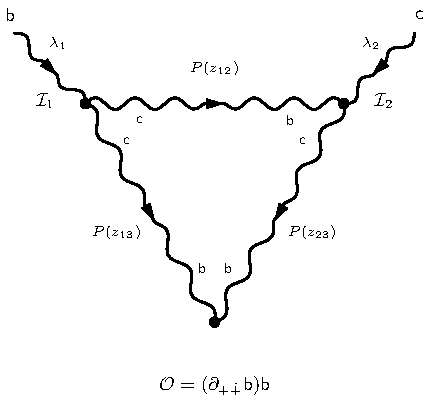
\includegraphics[width=0.62\linewidth,height=.70\textheight,keepaspectratio]{figures/feynarts/fa_N1_sources.pdf}
\caption{The displacement $z_{13}$ records the derivative on the first contracted field in $(\partial_{+\dot+}\mathsf b)\mathsf b$. The sources $\lambda_1,\lambda_2$ act on the surviving $\mathsf b$ and $\mathsf c$ fields.}
\label{fig:N1-sources}
\end{figure}

\end{minipage}\par

\noindent\begin{minipage}{\linewidth}
The $j$th term of the first line of \eqref{eq:1.7} places $K_{\varepsilon;e_j}$ on edge $e_j$ and $P_{\varepsilon,L}$ on every other edge. Figure~\ref{fig:N1-heat-markings} displays the three terms of the heat-edge sum for the triangle.
\begin{figure}[H]
\centering
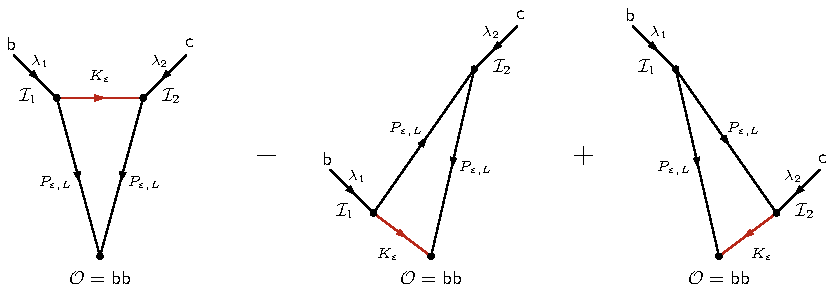
\includegraphics[width=0.99\linewidth,height=.70\textheight,keepaspectratio]{figures/feynarts/fa_N1_heat_markings.pdf}
\caption{The three heat-edge markings contributing to $Q_1(\mathsf b\mathsf b)$ in $\mathcal N=1$ Yang--Mills theory. The short red edge carries $K_\varepsilon$; the remaining internal edges carry $P_{\varepsilon,L}$. The signs follow the edge order $(12),(13),(23)$. Internal arrows run from $\mathsf c$ to $\mathsf b$. The external arrows are the sources $\lambda_1,\lambda_2$ of the surviving fields $\mathsf b,\mathsf c$.}
\label{fig:N1-heat-markings}
\end{figure}

\end{minipage}\par

For an oriented edge $e=(v,w)$, the propagator is
\begin{equation}\label{eq:C-explicit-propagator}
\begin{aligned}
[P_{\varepsilon,L;e}]_\Omega
={}&\frac{\epsilon_{\dot a\dot b}
 (x_v-x_w)^{-\dot a}d(x_v-x_w)^{-\dot b}}{32\pi^2}
 \int_\varepsilon^L\frac{dt_e}{t_e^3}\\
&\quad\times\exp\!\left[-\frac{
 (x_v-x_w+z_e)^{+\dot c}\epsilon_{\dot c\dot d}
 (x_v-x_w)^{-\dot d}}{2t_e}\right].
\end{aligned}
\end{equation}
As in \cite[Equations (2.16)--(2.17), (2.26)]{operatope}, with the normalization of \cite[Lemma 1, Equation (2.2)]{Wang}, we combine the antiholomorphic separations and Schwinger times into edge currents; this simplifies the integrand at the price of a more intricate integration region \cite[Section 2.3]{operatope}. Their pairing with the holomorphic coordinates in the exponent identifies them as the holomorphic momentum carried by each edge:
\begin{equation}\label{eq:1.8}
y_{e,+\dot a}
=\frac{\epsilon_{\dot a\dot b}
 (x_{e(0)}-x_{e(1)})^{-\dot b}}{2t_e},\qquad
 d^2y_e=dy_{e,+\dot+}\wedge dy_{e,+\dot-}.
\end{equation}
In these variables, the combined heat-kernel and propagator form in the third line of \eqref{eq:1.7} is
\begin{equation}\label{eq:C-current-Jacobian}
\begin{aligned}
[K_{t_e;e}]_\Omega
-dt_e\wedge[(Q^{\mathrm{GF}}\otimes1)K_{t_e;e}]_\Omega
={}&-\frac{e^{-(x_{e(0)}-x_{e(1)}+z_e)^{+\dot a}
 y_{e,+\dot a}}}{8\pi^2}\,d^2y_e.
\end{aligned}
\end{equation}
Substituting it into \eqref{eq:1.7} gives
\begin{equation}\label{eq:kernel-current-form}
\begin{aligned}
\mathcal I_\Gamma^{\mathrm{raw\ cut}}(\lambda;z)
={}&-\frac{1}{(8\pi^2)^{n+1}}\lim_{\varepsilon\downarrow0}
\int_{(\mathbb C^2)^{k-1}}
\left(\bigwedge_{v<k}\Omega_v\right)
e^{\sum_{v<k}\lambda_{v,+\dot a}x_v^{+\dot a}}\\
&\times\int_{\partial_{\mathrm{UV}}[\varepsilon,L]^{2n+1}}
e^{-\sum_{e\in\Gamma_1}(x_{e(0)}-x_{e(1)}+z_e)^{+\dot a}y_{e,+\dot a}}
\bigwedge_{e\in\Gamma_1}d^2y_e .
\end{aligned}
\end{equation}
This is the combined-propagator construction of
\cite[Section 2]{operatope}; the boundary integrals and their
holomorphic locality are established in \cite[Section 4, Proposition 9 and Theorem 6]{Wang}.

For real $\lambda_v$ and imaginary $z_e$, deforming the Gaussian contour
to imaginary $x_v^+$ and real $x_v^-$ gives the Fourier representation
of \cite[Section 2.7, Equations (2.31)--(2.32)]{operatope}. The exponent becomes
\begin{equation}\label{eq:C-fourier-exponent}
\begin{aligned}
&\sum_{v<k}\lambda_{v,+\dot a}x_v^{+\dot a}
-\sum_e(x_{e(0)}-x_{e(1)}+z_e)^{+\dot a}y_{e,+\dot a}\\
&\quad=-\sum_ez_e^{+\dot a}y_{e,+\dot a}
+\sum_{v<k}x_v^{+\dot a}
\left(\lambda_{v,+\dot a}
-\sum_{e:e(0)=v}y_{e,+\dot a}
+\sum_{e:e(1)=v}y_{e,+\dot a}\right).
\end{aligned}
\end{equation}
Each holomorphic-coordinate integral is therefore
\begin{equation}\label{eq:C-fourier-delta}
\begin{aligned}
&\int_{(i\mathbb R)^2}
\frac{dx_v^{+\dot+}\wedge dx_v^{+\dot-}}{(2\pi i)^2}
\exp\!\left[x_v^{+\dot a}
\left(\lambda_{v,+\dot a}
-\sum_{e:e(0)=v}y_{e,+\dot a}
+\sum_{e:e(1)=v}y_{e,+\dot a}\right)\right]\\
&\qquad=\prod_{\dot a=\dot+,\dot-}
\delta\!\left(\lambda_{v,+\dot a}
-\sum_{e:e(0)=v}y_{e,+\dot a}
+\sum_{e:e(1)=v}y_{e,+\dot a}\right).
\end{aligned}
\end{equation}
Thus the currents obey
\begin{equation}\label{eq:1.9}
\sum_{e:e(0)=v}y_{e,+\dot a}
-\sum_{e:e(1)=v}y_{e,+\dot a}
=\lambda_{v,+\dot a}.
\end{equation}
The result extends
coefficient by coefficient to the formal displacement and momentum
series. 
Collecting the remaining factors gives the current integral \eqref{eq:C-current-delta-integral} of Section~\ref{sec:setup}. The constants $(-8\pi^2)^n$ of \eqref{eq:1.7}, $(-1/8\pi^2)^{2n+1}$ of \eqref{eq:C-current-Jacobian} and the $n+1$ Gaussian integrals $\int\Omega_v\,e^{\cdots}=2(2\pi i)^2\delta^2=-8\pi^2\delta^2$ of \eqref{eq:C-fourier-delta} multiply to one, so the factor $(-1)^n$ is the sign of collecting the Schwinger differentials in \eqref{eq:1.7}.

\subsection{Network equations}
\label{sec:B-network}

The operatope kernel can be computed by reducing an electrical
network. The network equations are those of \cite[Equations (2.26), (2.31), (2.33)]{operatope}. The weighted Laplacian, Kirchhoff's matrix-tree theorem and the cut formulas behind the spanning-tree currents of Section~\ref{sec:B-spanning} are classical and appear for these integrals in \cite[Definition 12, Theorem 4, Corollaries 1--2, Remark 7]{Wang} and \cite[Appendix A]{GWW}; we recall them in network language. What we add is the iterated reduction of Sections~\ref{sec:B-local-reduction}--\ref{sec:B-general-forests}, which removes the spanning-tree denominator for fans, spiders and books, and for those forests whose eliminated trivalent vertices carry no source. For a connected graph $\Gamma$, let $\Gamma_0$ and
$\Gamma_1$ be its vertex and oriented edge sets. An edge $e=(v,w)$
has tail $e(0)=v$, head $e(1)=w$, resistance $t_e=t_{vw}$ and
current $y_{e,+\dot a}$. The prescribed external current
$\lambda_{v,+\dot a}$ enters at vertex $v$. Each dotted component
obeys the same network equations with one common set of resistances.
In the kernel, these external currents are the holomorphic momentum
sources.

For an oriented cycle $C$, Kirchhoff's current and voltage laws are
\[
\begin{aligned}
\sum_{e:e(0)=v}y_{e,+\dot a}
-\sum_{e:e(1)=v}y_{e,+\dot a}
&=\lambda_{v,+\dot a},
&\sum_{v\in\Gamma_0}\lambda_{v,+\dot a}&=0,\\
\sum_{\substack{e\in C\\\mathrm{along}\ C}}t_ey_{e,+\dot a}
-\sum_{\substack{e\in C\\\mathrm{against}\ C}}t_ey_{e,+\dot a}
&=0.
\end{aligned}
\]
These are \eqref{eq:1.9} and \eqref{eq:C-oriented-cycle}.
The vertex potential is $\epsilon_{\dot a\dot b}x_v^{-\dot b}/2$,
and \eqref{eq:1.8} is Ohm's law:
\[
t_ey_{e,+\dot a}
=\frac{\epsilon_{\dot a\dot b}
(x_{e(0)}-x_{e(1)})^{-\dot b}}2.
\]

At fixed external currents, every choice $t_e>0$ has a unique
current solution. Varying their ratios sweeps out the
operatope current domain at these sources. A common rescaling of
all resistances leaves the currents unchanged, so we may impose
$\sum_e t_e=1$. The boundary is obtained by limits in which some
normalized resistances vanish.

Choose a spanning tree $T$, which connects all vertices without a
cycle. Conservation determines its currents from those on the
remaining edges. Eliminating the tree currents in
\eqref{eq:C-current-delta-integral} has unit Jacobian: the grounded
incidence matrix of $T$ has determinant $\pm1$, and the two dotted
components square this sign. The kernel is therefore
\begin{equation}\label{eq:operatope}
\mathcal I_\Gamma^{\mathrm{raw\ cut}}(\lambda;z)
=\int_{\substack{y\in\Delta_\Gamma\\
\sum_{e:e(0)=v}y_e-\sum_{e:e(1)=v}y_e=\lambda_v}}
e^{-\sum_ez_e^{+\dot a}y_{e,+\dot a}}
\bigwedge_{e\notin T}(-dy_{e,+\dot+}\wedge dy_{e,+\dot-}).
\end{equation}
Here $\Delta_\Gamma$ carries the orientation induced by the heat-kernel
boundary in \eqref{eq:C-current-delta-integral}, and $z_e$ is the holomorphic displacement
on edge $e$. The differentials measure the change in the currents
as the resistances vary, with $\lambda$ held fixed. For an $n$-loop
graph there are $n$ edges outside $T$, giving the $2n$-dimensional
current form in this integral.

A self-loop resistor is shorted: both terminals lie at the same
potential. Since its Schwinger time is positive,
\[
t_ey_{e,+\dot a}=0,\qquad t_e>0
\quad\Longrightarrow\quad y_{e,+\dot a}=0,\qquad d^2y_e=0.
\]
For two parallel edges $e,e'$ of the original graph, oriented in the
same direction, the voltage drop is the same on both resistors:
\[
t_ey_{e,+\dot a}=t_{e'}y_{e',+\dot a},\qquad
 y_{e',+\dot a}=\frac{t_e}{t_{e'}}y_{e,+\dot a}.
\]
Their contribution to the full current form in
\eqref{eq:C-current-delta-integral} vanishes because every expanded
term repeats a current differential or $d(t_e/t_{e'})$:
\[
\begin{aligned}
d^2y_e\wedge d^2y_{e'}
={}&dy_{e,+\dot+}\wedge dy_{e,+\dot-}\\
&\wedge\left[\frac{t_e}{t_{e'}}dy_{e,+\dot+}
+y_{e,+\dot+}d\!\left(\frac{t_e}{t_{e'}}\right)\right]\\
&\wedge\left[\frac{t_e}{t_{e'}}dy_{e,+\dot-}
+y_{e,+\dot-}d\!\left(\frac{t_e}{t_{e'}}\right)\right]=0.
\end{aligned}
\]
The remaining sections construct coordinates in which these integrals
become elementary. Section~\ref{sec:B-spanning} gives the current
solution at fixed resistances, and Section~\ref{sec:B-forest-measure}
uses it to derive the measure for the marked graphs of the quantum
product. Series eliminations and parallel merges
(Section~\ref{sec:B-local-reduction}) give the dimensionless ratios
$r_j$, or $r_{i,j}$ along spider arms. Reversing these reductions
expresses the currents in coordinates whose domains are products of
intervals and simplices, with the conservation and cycle equations
already solved. Pulling back the original current form gives the
Jacobian, and expanding the displacement exponential reduces the kernel
to moments on these domains (Sections~\ref{sec:B-fan-reduction}--\ref{sec:book-jacobian}).
Section~\ref{sec:B-general-forests} treats general forests, Section~\ref{sec:B-short-circuits} proves the quadratic identities of the brackets in network language, and Section~\ref{sec:B-leibniz} reads the Leibniz rule of the quantum product directly off the marked circuits.

\subsection{Spanning-tree currents}
\label{sec:B-spanning}

For a fixed spanning tree $T\subset\Gamma_1$, the tree currents
$y^T_e$ obey conservation, with zero current on
the omitted edges $\Gamma_1\setminus T$. Deleting $e\in T$ splits
the tree into two components. Summing conservation over the component
containing $e(0)$ cancels its internal currents and gives $y^T_e$.
Here ``connected'' means joined by a path in $T\setminus\{e\}$,
irrespective of the arrows.

In \eqref{eq:operatope}, one chosen tree determines which currents
conservation eliminates. The sum below determines all currents at
fixed edge Schwinger times: each tree is weighted by the product of its
omitted-edge Schwinger times, and the denominator normalizes these weights.
The index $h$ in these products labels an edge. In cut form, the same current formula is \cite[Equation (3.1), Corollaries 1--2]{Wang}.

\par\noindent\begin{minipage}{\linewidth}
\begin{equation}\label{eq:1.24}
\begin{aligned}
y^T_{e,+\dot a}
&=\begin{cases}
\displaystyle\sum_{\substack{v\text{ connected to }e(0)\\
\text{in }T\setminus\{e\}}}\lambda_{v,+\dot a},&e\in T,\\[3pt]
0,&e\notin T,
\end{cases}\\[4pt]
y_{e,+\dot a}(t)
&=\frac{\displaystyle\sum_T
\left(\prod_{h\in\Gamma_1\setminus T}t_h\right)y^T_{e,+\dot a}}
{\displaystyle\sum_T\prod_{h\in\Gamma_1\setminus T}t_h}.
\end{aligned}
\end{equation}
\end{minipage}

Both outer sums run over every spanning tree of $\Gamma$.
At fixed resistances, the responses to separate external current
injections add: this is the superposition theorem of linear circuits.
Each injection is paired with its return current, so the total source
remains zero. On a tree, summing these responses gives the source sum
across the cut in \eqref{eq:1.24}. The weights depend only on the
resistances, and their normalized sum is one; hence the weighted
currents obey conservation at every vertex.

To check the voltage law, multiply each tree weight by the resistance
of the edge traversed by the cycle:
\[
t_e\prod_{h\in\Gamma_1\setminus T}t_h
=\prod_{h\in\Gamma_1\setminus(T\setminus\{e\})}t_h,
\qquad e\in T.
\]
\par\noindent\begin{minipage}{\linewidth}
Fix the two-component forest $T\setminus\{e\}$. Restoring any edge
between its components gives a spanning tree, and the displayed
weight is the same for every such choice. The signed tree current
in the cycle sum is the total source in the component from which
the cycle departs. Crossing back gives the opposite source sum,
since $\sum_v\lambda_{v,+\dot a}=0$. A closed cycle enters and leaves
each component equally often, so these terms cancel in pairs.
The triangle below shows one such pair.

\medskip
\centering
\BTreeCycleCancellationFigure
\captionof*{figure}{Cycle cancellation for the forest $\{12\}$.
The dashed separator divides its two components. Restoring $13$
or $23$ gives tree weights $t_{23}$ or $t_{13}$; multiplying by
the restored resistance gives the common weight $t_{13}t_{23}$.
The coloured terms are contributions to the numerator of the cycle
sum; their common denominator is $t_{12}+t_{13}+t_{23}$.
Each current denotes one fixed dotted component.}
\end{minipage}
\par\medskip
Grouping all terms this way proves the voltage law.
Thus \eqref{eq:1.24} satisfies both current equations; positive
resistances give a unique solution.

The same weights can be written using the conductances $t_h^{-1}$ of
the retained edges. Multiplication by $\prod_{h\in\Gamma_1}t_h$ gives
\begin{equation}\label{eq:tree-complement-weight}
\frac{\prod_{h\in T}t_h^{-1}}{\sum_{T'}\prod_{h\in T'}t_h^{-1}}
=\frac{\prod_{h\in\Gamma_1\setminus T}t_h}
{\sum_{T'}\prod_{h\in\Gamma_1\setminus T'}t_h}.
\end{equation}
Here $T'$ runs over the same spanning trees. Each tree omits
$|\Gamma_1|-|\Gamma_0|+1$ edges, so a common rescaling of all $t_e$
cancels in \eqref{eq:1.24}. We may therefore impose $\sum_e t_e=1$.

For the triangle, orient the edges as $1\to2$, $1\to3$ and $2\to3$,
with $\lambda_1+\lambda_2+\lambda_3=0$.
Figure~\ref{fig:spanning-trees} shows its three trees. They omit
$23$, $13$ and $12$, respectively, and have weights $t_{23}$,
$t_{13}$ and $t_{12}$. For example, in $T=\{12,13\}$ the component
of vertex $1$ after deleting $12$ is $\{1,3\}$; hence
$y^T_{12,+\dot a}=\lambda_{1,+\dot a}+\lambda_{3,+\dot a}
=-\lambda_{2,+\dot a}$. Substituting these three tree currents and weights into \eqref{eq:1.24} gives
\par\noindent\begin{minipage}{\linewidth}
\par\smallskip
\begingroup\captionsetup{hypcap=false}\centering
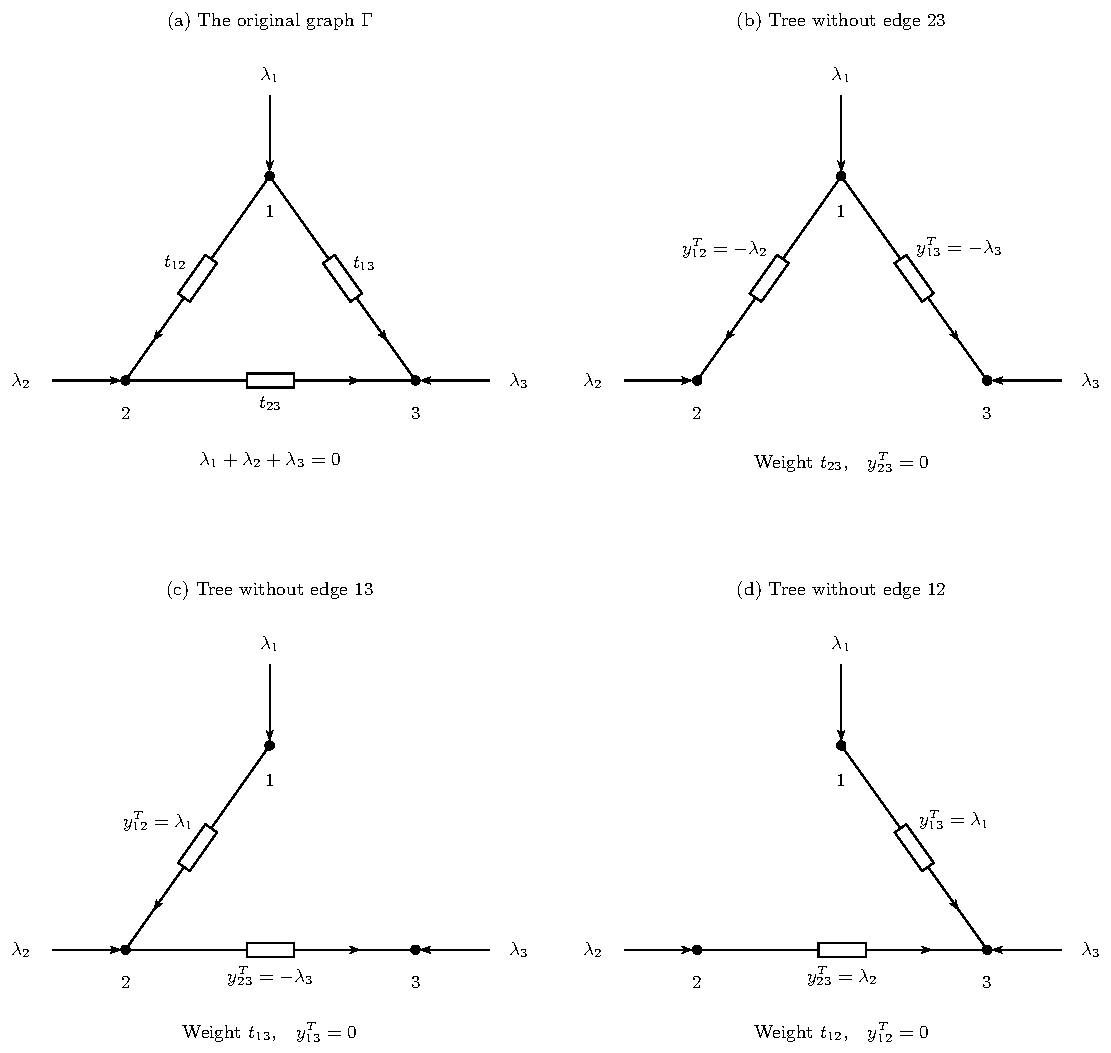
\includegraphics[width=.82\linewidth]{figures/circuits/triangle_tree_currents.pdf}
\captionof{figure}{The triangle circuit and its spanning trees in \eqref{eq:1.24}. Here $\Gamma_1=\{12,13,23\}$. Each edge carries a resistor; the tree panels label their currents. Each omitted edge has zero tree current, and its Schwinger time supplies the displayed weight. The common index $+\dot a$ is suppressed.}
\label{fig:spanning-trees}
\par\endgroup

\begin{equation}\label{eq:tree-triangle-currents}
\begin{aligned}
y_{12,+\dot a}
&=\frac{t_{13}\lambda_{1,+\dot a}-t_{23}\lambda_{2,+\dot a}}
{t_{12}+t_{13}+t_{23}},\\
y_{13,+\dot a}
&=\frac{(t_{12}+t_{23})\lambda_{1,+\dot a}+t_{23}\lambda_{2,+\dot a}}
{t_{12}+t_{13}+t_{23}},\\
y_{23,+\dot a}
&=\frac{t_{13}\lambda_{1,+\dot a}+(t_{12}+t_{13})\lambda_{2,+\dot a}}
{t_{12}+t_{13}+t_{23}}.
\end{aligned}
\end{equation}
\end{minipage}
\par
Directly,
\begin{equation}\label{eq:tree-triangle-check}
\begin{aligned}
y_{12,+\dot a}+y_{13,+\dot a}&=\lambda_{1,+\dot a},&
-y_{12,+\dot a}+y_{23,+\dot a}&=\lambda_{2,+\dot a},\\
t_{12}y_{12,+\dot a}+t_{23}y_{23,+\dot a}-t_{13}y_{13,+\dot a}&=0.
\end{aligned}
\end{equation}
In the gauge $t_{12}+t_{13}+t_{23}=1$, substituting
$(t_{12},t_{13},t_{23})=(1-r_1-r_2,r_1,r_2)$ recovers the
triangle currents in Section~\ref{sec:fans}.

\subsection{The marked-forest measure}
\label{sec:B-forest-measure}

To evaluate a marked-graph contribution to the quantum product
\eqref{eq:star}, we need its kernel as an integral over edge
resistances. Equation~\eqref{eq:1.24} gives the currents in terms of
these resistances. We now compute the Jacobian of this change of
variables. For an interaction forest, its numerator factors into
one antisymmetric pair of currents at each interaction vertex.
The edge assignment below identifies these pairs: in every nonzero term of the numerator, each physical edge is given to one of its interaction endpoints, and each interaction vertex receives two edges.

\Needspace{6\baselineskip}
The local operators $A,B$ occupy the insertion vertices
$A=n+1$, $B=n+2$; the other $n$ vertices carry interactions.
The full marked graph has $2n$ physical contractions and the auxiliary
edge $AB$ of \eqref{eq:star}, carrying the mark $\gamma$.
An internal edge joins two interaction vertices; a spoke joins an
interaction vertex to either insertion.

\par\noindent\begin{minipage}{\linewidth}
Deleting $A,B$ and all their incident edges leaves the interaction
graph. For the contributing graphs of \eqref{eq:1.19}, it is a
\emph{forest}: a disjoint union of connected trees $T_j$, each without
a cycle. An isolated vertex is also a tree. Figure~\ref{fig:B-forest-assignment}
shows two two-loop examples, with one and two components respectively.
For a component $T_j$, $|T_j|$ counts its vertices; it has $|T_j|-1$
internal edges and $|T_j|+1$ spokes. Thus $2|T_j|$ physical edges
must be paired among its interaction vertices.
\label{par:B-forest-introduction}
\par\smallskip
\begingroup\captionsetup{hypcap=false}\centering
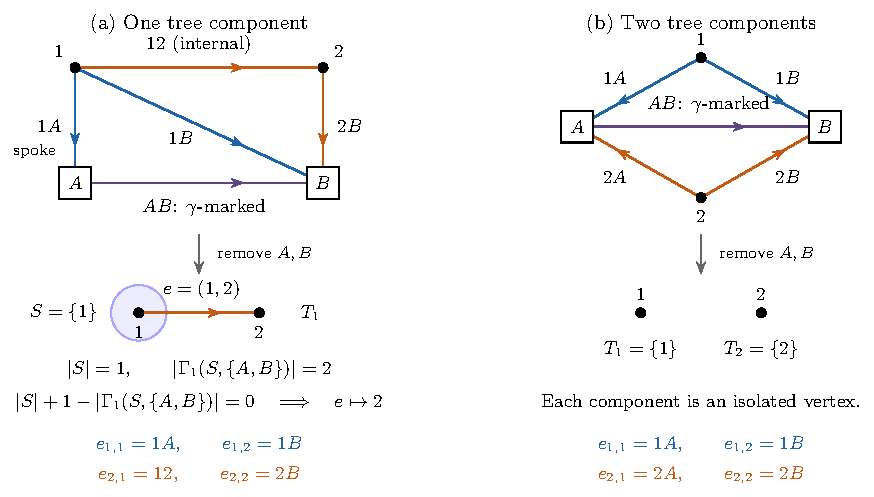
\includegraphics[width=.94\linewidth]{figures/forest_edge_assignment.pdf}
\captionof{figure}{Two-loop marked graphs for the quantum product. Squares are the operator insertions $A,B$; dots carry interactions. Removing the insertions leaves the displayed forest. In (a), $S=\{1\}$ is the component containing the tail of $12$ after cutting that edge. Blue and orange identify the pairs assigned to vertices $1$ and $2$, listed as $e_{v,1}<e_{v,2}$ in physical-edge order. Arrows orient currents; the purple $AB$ edge carries the auxiliary mark.}
\label{fig:B-forest-assignment}
\par\endgroup\medskip

\end{minipage}
\par\medskip

\Needspace{18\baselineskip}
\begin{proposition}[Edge assignment for the forest measure]
\label{prop:B-forest-assignment}
Let $\Gamma$ be a marked Laman graph whose interaction subgraph is
an interaction forest as above. There is a unique assignment of
every physical edge to one of its interaction endpoints such that
each interaction vertex receives exactly two edges.
Every spoke is assigned to its interaction endpoint.
For an internal edge $e$ of $T_j$, let $S$ be the component of
$T_j\setminus\{e\}$ containing its tail $e(0)$, and let
$\Gamma_1(S,\{A,B\})$ be the set of spokes from $S$ to the insertions.
The assignment is
\begin{equation}\label{eq:1.27}
\begin{gathered}
0\leq|S|+1-|\Gamma_1(S,\{A,B\})|\leq1,\\
e\longmapsto\begin{cases}
e(0),&|S|+1-|\Gamma_1(S,\{A,B\})|=1,\\
e(1),&|S|+1-|\Gamma_1(S,\{A,B\})|=0.
\end{cases}
\end{gathered}
\end{equation}
\end{proposition}
The column of a resistor in the Jacobian numerator has entries only in the rows of its interaction end nodes: scaling its conductance at fixed node potentials changes the current fed into each end node by $\pm$ its own current. A nonzero term lets every interaction node take up two resistors, one per dotted component; in a forest this sharing is unique: a spoke goes to its interaction node, and an internal resistor to the side of the tree that is one resistor short (Figure~\ref{fig:B-assignment-count}).

\begin{proof}
The internal resistors of $S$, its spokes and the marked resistor $AB$
form the subcircuit on $S\cup\{A,B\}$, and the local count of Ohm's law
(Theorem~\ref{thm:laman-subgraph}) gives
\[
\underbrace{|S|-1}_{\text{internal resistors in }S}
+\underbrace{|\Gamma_1(S,\{A,B\})|}_{\text{spokes from }S}
+\underbrace{1}_{AB}
\le 2(|S|+2)-3,
\]
so $|\Gamma_1(S,\{A,B\})|\le |S|+1$. Applying the same bound to the
other component and using the total of $|T_j|+1$ spokes gives
\[
\begin{aligned}
|\Gamma_1(S,\{A,B\})|
&=|T_j|+1-|\Gamma_1(T_j\setminus S,\{A,B\})|\\
&\ge |T_j|+1-(|T_j|-|S|+1)=|S|.
\end{aligned}
\]
An internal resistor with both ends in $S$, and a spoke from $S$,
have all their interaction ends in $S$, so each is given to a
node of $S$. They supply the nodes of $S$ with
$|S|-1+|\Gamma_1(S,\{A,B\})|$ resistors. The nodes of $S$ need $2|S|$,
and the only other resistor at $S$ is the cut resistor $e$.
The deficit of $S$, the number of resistors it still lacks, must
therefore come from $e$:
\[
\underbrace{2|S|}_{\text{needed}}
-\underbrace{\bigl(|S|-1+|\Gamma_1(S,\{A,B\})|\bigr)}_{\text{supplied within }S}
=|S|+1-|\Gamma_1(S,\{A,B\})|\in\{0,1\}.
\]
If the deficit is one, $e$ is given to its endpoint $e(0)$ in $S$;
if it is zero, to $e(1)$ (Figure~\ref{fig:B-assignment-count}(b),(c)).
This is \eqref{eq:1.27} and proves uniqueness.

To check that this rule gives two resistors to every node $v$, remove
$v$ from $T_j$. For each remaining component $S$, its single resistor
to $v$ is given to $v$ precisely when $S$ has no deficit, that is,
when its own internal resistors and spokes already give two resistors to each
of its nodes (Figure~\ref{fig:B-assignment-count}(d)). It therefore
gives $|\Gamma_1(S,\{A,B\})|-|S|\in\{0,1\}$ resistors to $v$. Adding the spokes at $v$ gives
\[
\begin{aligned}
&|\Gamma_1(\{v\},\{A,B\})|
+\sum_{\substack{S\text{ a component}\\\text{of }T_j\setminus\{v\}}}
\bigl(|\Gamma_1(S,\{A,B\})|-|S|\bigr)\\
&\qquad=(|T_j|+1)-(|T_j|-1)=2.
\end{aligned}
\]
This also covers a single-node tree, for which the sum is empty.
\end{proof}
\begin{figure}[H]
\centering
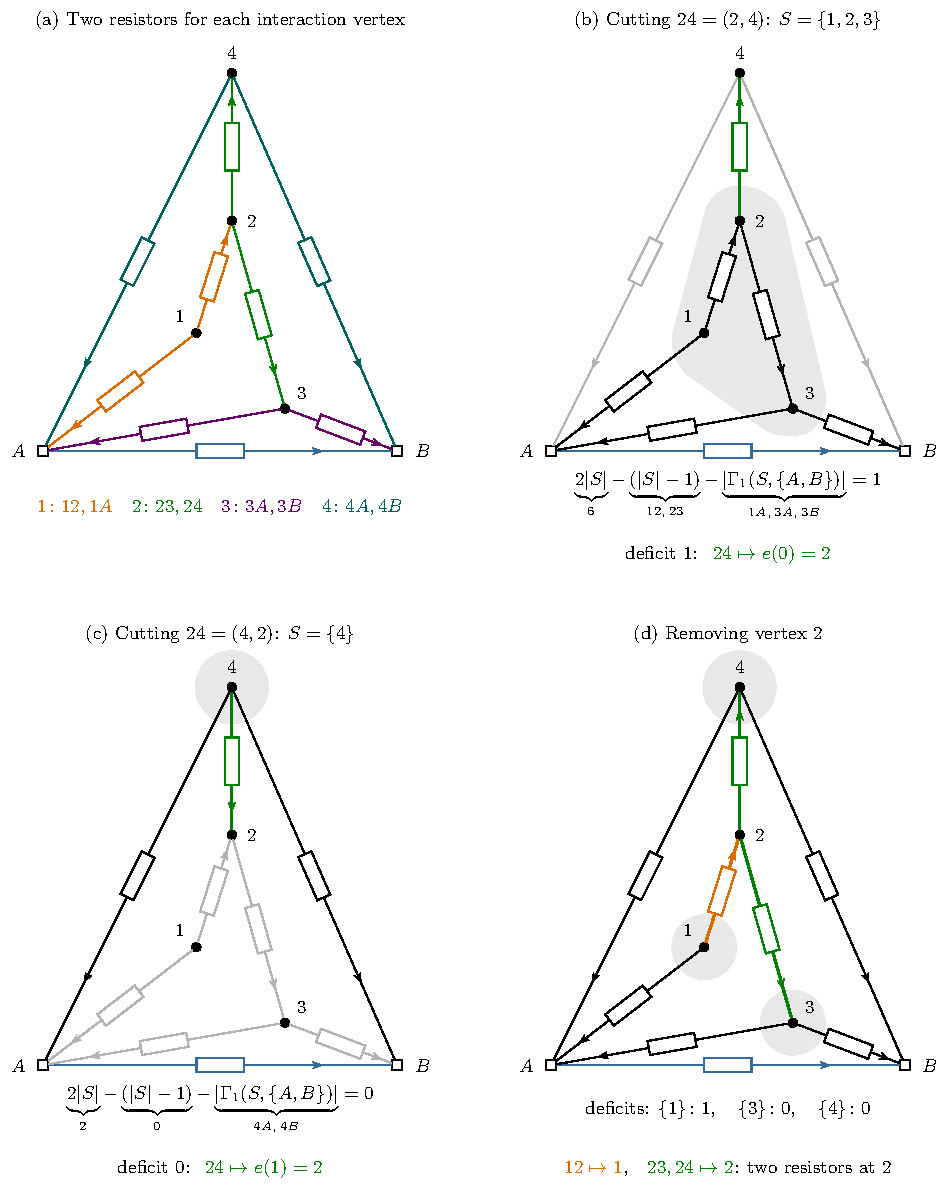
\includegraphics[width=\linewidth,height=.80\textheight,keepaspectratio]{figures/circuits/forest_assignment_count.pdf}
\caption{The edge assignment for the four-loop forest of Figure~\ref{fig:forest-star-triangle}. (a) Each interaction vertex receives two resistors, drawn in its colour. (b), (c) The cut resistor $24$ seen from its two ends: the shaded component $S$ containing the tail supplies itself with its internal resistors and spokes, and the cut resistor covers the deficit. With the tail at $2$, $S=\{1,2,3\}$ lacks one resistor and $24$ goes to $e(0)=2$; with the tail at $4$, $S=\{4\}$ lacks none and $24$ goes to $e(1)=2$. (d) The check at vertex $2$: of the components $\{1\},\{3\},\{4\}$ left by removing $2$, only $\{1\}$ has a deficit, so $12$ goes to $1$ and $23,24$ go to $2$.}
\label{fig:B-assignment-count}
\end{figure}

\paragraph{From the assignment to the kernel.}
The Jacobian numerator has two rows per interaction vertex,
ordered as $(1,\dot+),(1,\dot-),\ldots,(n,\dot+),(n,\dot-)$,
and one column per physical edge in its original order. The entry of
edge $e$ in the rows of $v$ is
$(\delta_{v,e(0)}-\delta_{v,e(1)})y_{e,+}{}^{\dot a}$, where
$\delta_{v,e(0)}-\delta_{v,e(1)}$ is $+1$ for an edge directed away
from $v$ and $-1$ for an edge directed towards $v$; it vanishes unless
$v$ is an endpoint of $e$. For the two-loop graph of
Figure~\ref{fig:B-forest-assignment}(a), with ordered edges
$(1A,1B,12,2B,AB)$, where $12$ means the edge $1\to2$, and similarly
for the other labels,
\[
\det\left(\begin{array}{cc|cc}
y_{1A,+}{}^{\dot+}&y_{1B,+}{}^{\dot+}&y_{12,+}{}^{\dot+}&0\\
y_{1A,+}{}^{\dot-}&y_{1B,+}{}^{\dot-}&y_{12,+}{}^{\dot-}&0\\\hline
0&0&-y_{12,+}{}^{\dot+}&y_{2B,+}{}^{\dot+}\\
0&0&-y_{12,+}{}^{\dot-}&y_{2B,+}{}^{\dot-}
\end{array}\right)
=\underbrace{\bigl(y_{1A,+\dot a}y_{1B,+}{}^{\dot a}\bigr)}_{\text{vertex }1:\ 1A,\,1B}
\underbrace{\bigl(-y_{12,+\dot b}y_{2B,+}{}^{\dot b}\bigr)}_{\text{vertex }2:\ 12,\,2B}.
\]
The component $S=\{1\}$ has its two spokes, so its deficit is zero and
$12$ is given to vertex $2$; the only entry outside the two diagonal
blocks is that of $12$ in the rows of its tail $1$, and the matrix is
block triangular. Each block is the antisymmetric pair of the two
currents given to its vertex,
$y^{\dot+}w^{\dot-}-y^{\dot-}w^{\dot+}=y_{+\dot a}w_+{}^{\dot a}$.

In general, denote the two resistors kept by $v$ by
$e_{v,1}<e_{v,2}$ in the original order. A column has nonzero
entries only in the rows of the interaction ends of its resistor, at
most four. Order the columns as
$(e_{1,1},e_{1,2},\ldots,e_{n,1},e_{n,2})$ and orient each internal
resistor towards the node that keeps it. An entry outside the diagonal
blocks then lies in the rows of the tail of such a resistor: each node keeps
two of its resistors, and a resistor between two nodes also appears at the
node that does not keep it. Along the trees of internal resistors the nodes
can be ordered with every tail before its head, and the matrix becomes block
triangular with the $2\times2$ blocks of the kept pairs. The numerator factors as
\[
\begin{aligned}
&\det_{(v\le n,\dot a),\,e\ne AB}
\left[(\delta_{v,e(0)}-\delta_{v,e(1)})y_{e,+}{}^{\dot a}\right]\\
&\quad=\sgn(e_{1,1},e_{1,2},\ldots,e_{n,1},e_{n,2})
\prod_{v=1}^n\left[
\prod_{b=1}^2(\delta_{v,e_{v,b}(0)}-\delta_{v,e_{v,b}(1)})
y_{e_{v,1},+\dot a_v}y_{e_{v,2},+}{}^{\dot a_v}\right].
\end{aligned}
\]
The remaining sign is the sign of the permutation from the
physical-edge order to $(e_{1,1},e_{1,2},\ldots,e_{n,1},e_{n,2})$.
Once the currents are known, the numerator costs $n$ two-by-two
determinants.

Choose a spanning tree $T$ containing $AB$ to select the independent
currents in \eqref{eq:operatope}. In the gauge
$t_{AB}=1-\sum_{e\ne AB}t_e>0$, the independent resistances are those
of the $2n$ physical edges. The pullback of the oriented current
measure is
\[
\begin{aligned}
&\bigwedge_{e\notin T}
\left(-dy_{e,+\dot+}\wedge dy_{e,+\dot-}\right)\\
&\qquad=
\frac{\displaystyle
\det_{(v\le n,\dot a),\,e\ne AB}
\left[(\delta_{v,e(0)}-\delta_{v,e(1)})y_{e,+}{}^{\dot a}\right]}
{\displaystyle t_{AB}\left(\sum_{T'}\prod_{h\notin T'}t_h\right)^2}
\bigwedge_{e\ne AB}dt_e.
\end{aligned}
\]
Here $T'$ runs over all spanning trees, as in \eqref{eq:1.24},
and both wedge products carry the edge ordering of
\eqref{eq:operatope}. Inserting the factorized determinant gives
\begin{equation}\label{eq:forestuniform}
\begin{aligned}
\mathcal I_\Gamma^{\mathrm{raw\ cut}}(\lambda;z)
={}&\sgn(e_{1,1},e_{1,2},\ldots,e_{n,1},e_{n,2})
\int_{\substack{t_e>0\\\sum_{e\ne AB}t_e<1}}\prod_{e\ne AB}dt_e\\
&\times\frac{\displaystyle\prod_{v=1}^n
\left[\prod_{b=1}^2(\delta_{v,e_{v,b}(0)}-\delta_{v,e_{v,b}(1)})
y_{e_{v,1},+\dot a_v}y_{e_{v,2},+}{}^{\dot a_v}\right]}
{\displaystyle t_{AB}\left(\sum_T\prod_{h\notin T}t_h\right)^2}
e^{-\sum_e y_{e,+\dot a}z_e^{+\dot a}}.
\end{aligned}
\end{equation}
Thus \eqref{eq:1.24} supplies every current in the integrand, while
\eqref{eq:1.27} fixes its numerator and sign. This is the
kernel multiplying the physical contractions of the marked graph
in the quantum-product expansion. Its denominator contains the square of the tree polynomial, as does the integrand in the proof of \cite[Theorem 6]{Wang} on $\mathbb C^2$, and its currents \eqref{eq:1.24} have the tree polynomial as denominator, as in \cite[Corollaries 1--2]{Wang}. For spiders and books, and for those forests whose eliminated trivalent vertices carry no source, the reductions below remove these denominators.

For Figure~\ref{fig:B-forest-assignment}(a) the permutation sign is
$+1$ and the numerator in \eqref{eq:forestuniform} is the product of
the two blocks above. For panel (b), each isolated interaction vertex
receives its two spokes; in the order $(1A,1B,2A,2B,AB)$ the matrix
is block diagonal, every incidence factor is positive, and the
numerator is
\[
\bigl(y_{1A,+\dot a}y_{1B,+}{}^{\dot a}\bigr)
\bigl(y_{2A,+\dot b}y_{2B,+}{}^{\dot b}\bigr).
\]

In Schwinger times the cost lies in the currents. Every current in
\eqref{eq:1.24} and the denominator of \eqref{eq:forestuniform} are
sums over all spanning trees, and their number grows exponentially
with the loop order: $2^{n-1}(n+2)$ for the $n$-page book with its
marked edge ($8$ at two loops, $1280$ at eight), and the Fibonacci
number $F_{2n+2}$ for the $n$-loop fan of Section~\ref{sec:fans}
($8$ and $2584$). At fixed resistances the currents follow from one
linear solve, but as functions to be integrated,
\eqref{eq:forestuniform} is a rational function with exponentially
many terms on a $2n$-dimensional simplex. The reductions of
Sections~\ref{sec:B-local-reduction}--\ref{sec:B-general-forests}
remove the spanning-tree sums: for fans, spiders and books the density
becomes a product of powers of the reduction coordinates and of their
complements, \eqref{eq:1.40}, \eqref{eq:1.53} and \eqref{eq:B-book-full-kernel},
and the currents are polynomials in these coordinates. Each term of
the resulting expansions is a product of $O(n)$ ratios of factorials;
Table~\ref{tab:B-costs} compares the two descriptions. The number of terms of the expansion is the same in both: at zero displacement it is the number of terms of the momentum polynomial, the product of source pairings in the density, which is $1$ for the fan, $\prod_i\binom{\ell_i+a-1}{a-1}$ for a spider and $n^n$ for a book with a source on every page, and each degree of displacement multiplies it by at most $O(n^2)$.

\begin{table}[H]
\centering\small
\caption{Cost of one exact coefficient of the kernel at $n$ loops and displacement degree $m$. In Schwinger times the integrand has a power of the tree polynomial $\sum_T\prod_{h\notin T}t_h$, one monomial per spanning tree, as denominator \eqref{eq:forestuniform}; in the circuit coordinates the density is polynomial.}
\label{tab:B-costs}
\begin{tabular}{>{\raggedright\arraybackslash}p{.2\linewidth}>{\raggedright\arraybackslash}p{.27\linewidth}>{\raggedright\arraybackslash}p{.43\linewidth}}
\toprule
Graphs&Monomials of the tree polynomial (original method)&One coefficient, circuit coordinates\\
\midrule
fan, $n$ loops&$F_{2n+2}\sim2.62^n$&closed form at zero displacement, \eqref{eq:1.42}; $O(n(m+1)^2)$ per coefficient in the pairings, linear in $n$, Lemma~\ref{lem:fan-recursion}\\[3pt]
spider, arms $\ell_1,\ldots,\ell_a$&between book and fan&one product of factorial ratios per term of \eqref{eq:spider-full-taylor}, $O(n+m)$\\[3pt]
book, $n$ pages&$2^{n-1}(n+2)$&one product of factorial ratios per term, $O(n+m)$, \eqref{eq:B-book-full-kernel}\\[3pt]
type I$'$ forests&exponential&spider density with the reduced current \eqref{eq:product-typeI-current}; one product of factorial ratios per term, $O(n+m)$\\[3pt]
other cubic forests&exponential&block-triangular Jacobian; one product of factorial ratios per term, $O(n+m)$\\[3pt]
sourced trivalent vertices&exponential&rational currents; convergent series \eqref{eq:1.81}\\
\bottomrule
\end{tabular}
\end{table}

\begingroup
\setlength{\abovedisplayskip}{7pt plus 2pt minus 2pt}
\setlength{\belowdisplayskip}{7pt plus 2pt minus 2pt}
\setlength{\abovedisplayshortskip}{3pt plus 2pt}
\setlength{\belowdisplayshortskip}{7pt plus 2pt minus 2pt}
\subsection{Series and parallel resistance reductions}\label{sec:B-local-reduction}

We construct the reduction coordinates by eliminating a vertex
and merging the resulting parallel edges. Reversing each reduction restores a solution of the original
conservation and cycle equations. Uniqueness identifies it with
\eqref{eq:1.24}; the reduction fractions give coordinates for the
fan and spider integrals.

Superscript $\mathrm{red}$ denotes the network after the indicated
elimination or parallel merge. Suppose $v$ has exactly two neighbours, $u,w$.
Conservation at $v$ and the coordinate difference between $u,w$ give
\begin{equation}\label{eq:B-series-derivation}
\begin{aligned}
y_{vu,+\dot a}+y_{vw,+\dot a}&=\lambda_{v,+\dot a},\\
\frac{\epsilon_{\dot a\dot b}(x_u-x_w)^{-\dot b}}2
&=-t_{vu}y_{vu,+\dot a}+t_{vw}y_{vw,+\dot a}\\
&=t_{vw}\lambda_{v,+\dot a}-(t_{vu}+t_{vw})y_{vu,+\dot a}.
\end{aligned}
\end{equation}
The two resistances add in series (Figure~\ref{fig:B-local-reduction}). The replacement edge $u\to w$ has resistance
$t_{vu}+t_{vw}$ and current
$\epsilon_{\dot a\dot b}(x_u-x_w)^{-\dot b}/[2(t_{vu}+t_{vw})]$.
At $u$, replacing $-y_{vu}$ by $y_{uw}^{\mathrm{red}}$ increases
the outgoing current by $t_{vw}\lambda_v/(t_{vu}+t_{vw})$;
at $w$ the increase is $t_{vu}\lambda_v/(t_{vu}+t_{vw})$.
\par\noindent\begin{minipage}{\linewidth}
Label this elimination step by $j$ and write its Schwinger-time fraction as $r_j$:
\begin{equation}\label{eq:1.64}
\begin{gathered}
r_j=\frac{t_{vu}}{t_{vu}+t_{vw}},\qquad
t_{uw}^{\mathrm{red}}=t_{vu}+t_{vw},\\
\lambda_{u,+\dot a}^{\mathrm{red}}
=\lambda_{u,+\dot a}+(1-r_j)\lambda_{v,+\dot a},\qquad
\lambda_{w,+\dot a}^{\mathrm{red}}
=\lambda_{w,+\dot a}+r_j\lambda_{v,+\dot a},\\
y_{vu,+\dot a}=(1-r_j)\lambda_{v,+\dot a}-y_{uw,+\dot a}^{\mathrm{red}},\qquad
y_{vw,+\dot a}=r_j\lambda_{v,+\dot a}+y_{uw,+\dot a}^{\mathrm{red}}.
\end{gathered}
\end{equation}

\par\smallskip
\begingroup\captionsetup{hypcap=false}\centering
\resizebox{.97\linewidth}{!}{\BLocalReductionFigure}
\captionof{figure}{Series elimination \eqref{eq:1.64} followed by a parallel merge.
Eliminating $v$ redistributes its source between $u$ and $w$.
The middle graph has $q=2$ parallel edges: edge $j=1$ replaces
the path through $v$, with $t_{uw}^{(1)}=t_{vu}+t_{vw}$;
edge $j=2$ is the original edge, with $t_{uw}^{(2)}=t_{uw}$.
Their currents add when the two edges merge.}
\label{fig:B-local-reduction}
\par\endgroup
\end{minipage}


\par\noindent\begin{minipage}{\linewidth}
We now replace $q$ parallel resistors between $u$ and $w$ by a
single effective edge, carrying their total current at the same
voltage. Orient all $q$ edges from $u$ to $w$ and label them
by $j=1,\ldots,q$.
The $j$th edge has Schwinger time $t_{uw}^{(j)}$ and current
$y_{uw,+\dot a}^{(j)}$; the superscript $(j)$ identifies the edge.
All $q$ edges have the same coordinate difference, so
\begin{equation}\label{eq:B-parallel-derivation}
\begin{aligned}
t_{uw}^{(j)}y_{uw,+\dot a}^{(j)}
&=\frac{\epsilon_{\dot a\dot b}(x_u-x_w)^{-\dot b}}2,\\
y_{uw,+\dot a}^{\mathrm{red}}
&=\sum_{j=1}^q y_{uw,+\dot a}^{(j)}
=\left(\sum_{j=1}^q\frac1{t_{uw}^{(j)}}\right)
\frac{\epsilon_{\dot a\dot b}(x_u-x_w)^{-\dot b}}2.
\end{aligned}
\end{equation}
The merged current is their sum. The parallel resistance is fixed by adding
the conductances $1/t_{uw}^{(j)}$. For this merge, $r_j$ is the
fraction of the total conductance carried by edge $j$:
\begin{equation}\label{eq:1.63}
\begin{gathered}
\frac1{t_{uw}^{\mathrm{red}}}=\sum_{j=1}^q\frac1{t_{uw}^{(j)}},\qquad
r_j=\frac{t_{uw}^{\mathrm{red}}}{t_{uw}^{(j)}},\qquad\sum_{j=1}^q r_j=1,\\
y_{uw,+\dot a}^{(j)}=r_jy_{uw,+\dot a}^{\mathrm{red}}.
\end{gathered}
\end{equation}


\end{minipage}
\par\endgroup

\subsection{Reduction moves as kernel recursions}\label{sec:B-kernel-recursion}

A series step followed by the parallel merge that it creates removes one node and one loop, and so does a star--triangle move at a node without source when two sides of the new triangle merge with resistors already present. Each move turns the kernel of a circuit into an integral of the kernel of the smaller circuit over the current-division ratios of the move (Figure~\ref{fig:kernel-moves}). A pairing of currents written in front of a kernel is inserted under its current integral, each $y^{\mathrm{red}}_{e,+\dot a}$ acting as $-\partial/\partial z^{\mathrm{red},+\dot a}_e$ (Remark~\ref{rem:circuit}).

\begin{figure}[H]
\centering
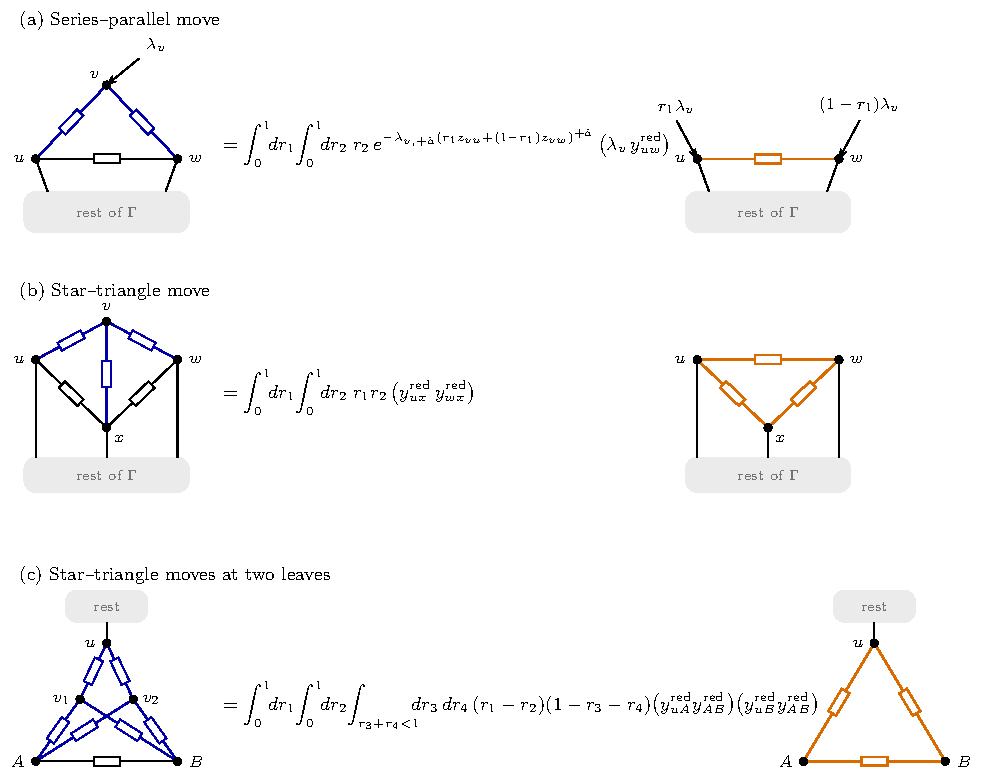
\includegraphics[width=\linewidth]{figures/circuits/kernel_moves.pdf}
\caption{The reduction moves as kernel recursions. Blue: the resistors removed by the move; orange: the new or merged resistors of the reduced circuit. (a) A node with two resistors whose ends are joined (Theorem~\ref{thm:kernel-series-parallel}): its source is passed on in the ratio $r_1:(1-r_1)$, and the merged resistor carries the current $y^{\mathrm{red}}_{uw}$. (b) A node without source whose star closes two triangles with resistors already present (Theorem~\ref{thm:kernel-star-triangle}). (c) Two leaves without sources wired to $u$, $A$ and $B$, with $A$ and $B$ joined and $u$ wired to neither (Theorem~\ref{thm:kernel-two-leaves}).}
\label{fig:kernel-moves}
\end{figure}

\begin{theorem}[Series--parallel move]\label{thm:kernel-series-parallel}
Let the node $v$ of a Laman circuit $\Gamma$ carry the source $\lambda_v$ and exactly two resistors, to $u$ and to $w$, and let a resistor join $u$ to $w$. Orient $vu,vw$ away from $v$ and $uw$ from $u$ to $w$, and order the resistors of $\Gamma$ with $vu,vw$ first. Eliminating $v$ in series and merging the new resistor with $uw$ in parallel (Proposition~\ref{prop:fan-step}) leaves the circuit $\Gamma^{\mathrm{red}}$: the remaining resistors in their order, the merged resistor in place of $uw$, and the sources
\[
\lambda^{\mathrm{red}}_u=\lambda_u+r_1\lambda_v,\qquad
\lambda^{\mathrm{red}}_w=\lambda_w+(1-r_1)\lambda_v,\qquad
r_1=\frac{t_{vw}}{t_{vu}+t_{vw}},\qquad
r_2=\frac{t_{vu}+t_{vw}}{t_{vu}+t_{vw}+t_{uw}} .
\]
Then
\begin{equation}\label{eq:kernel-series-parallel}
\mathcal I^{\mathrm{raw\ cut}}_\Gamma(\lambda;z)
=\int_0^1\!dr_1\int_0^1\!dr_2\;r_2\,
e^{-\lambda_{v,+\dot a}\left(r_1z_{vu}+(1-r_1)z_{vw}\right)^{+\dot a}}
\bigl(\lambda_{v,+\dot a}\,y^{\mathrm{red}}_{uw,+}{}^{\dot a}\bigr)\,
\mathcal I^{\mathrm{raw\ cut}}_{\Gamma^{\mathrm{red}}}\bigl(\lambda^{\mathrm{red}};z^{\mathrm{red}}\bigr),
\end{equation}
with $z^{\mathrm{red}}_{uw}=r_2z_{uw}+(1-r_2)(z_{vw}-z_{vu})$ and $z^{\mathrm{red}}_e=z_e$ for the other resistors.
\end{theorem}
\begin{proof}
\emph{Resistances.} The series sum and the parallel merge give
\[
t_{vw}=\frac{r_1\,t^{\mathrm{red}}_{uw}}{1-r_2},\qquad
t_{vu}=\frac{(1-r_1)\,t^{\mathrm{red}}_{uw}}{1-r_2},\qquad
t_{uw}=\frac{t^{\mathrm{red}}_{uw}}{r_2},
\]
so the resistance ratios of $\Gamma$ are $(r_1,r_2)\in(0,1)^2$ together with those of $\Gamma^{\mathrm{red}}$. The Jacobian of $(t_{vu},t_{vw},t_{uw})$ with respect to $(r_1,r_2,t^{\mathrm{red}}_{uw})$ is $-(t^{\mathrm{red}}_{uw})^2/[r_2^2(1-r_2)^3]$; with the stated orders, $\eta_\Gamma$ is a negative multiple of $dr_1\wedge dr_2\wedge\eta_{\Gamma^{\mathrm{red}}}$.

\emph{Currents.} The source of $v$ reaches $u$ and $w$ in the ratio $r_1:(1-r_1)$, every resistor of $\Gamma^{\mathrm{red}}$ other than $uw$ carries the same current in $\Gamma$, and the merged current divides between $uw$ and the path through $v$ (Proposition~\ref{prop:fan-step}):
\[
y_{uw}=r_2\,y^{\mathrm{red}}_{uw},\qquad
y_{vu}=r_1\lambda_v-(1-r_2)\,y^{\mathrm{red}}_{uw},\qquad
y_{vw}=\lambda_v-y_{vu}.
\]

\emph{Displacements.} Substituting these currents,
\[
\sum_{e\in\Gamma_1}z_e^{+\dot a}y_{e,+\dot a}
=\lambda_{v,+\dot a}\bigl(r_1z_{vu}+(1-r_1)z_{vw}\bigr)^{+\dot a}
+\sum_{e\in\Gamma^{\mathrm{red}}_1}z^{\mathrm{red},+\dot a}_e\,y^{\mathrm{red}}_{e,+\dot a}:
\]
the transferred source travels along $vu$ and $vw$, and the merged current along $uw$ and $u\to v\to w$.

\emph{Loop currents.} $\Gamma$ has one loop more than $\Gamma^{\mathrm{red}}$, the loop through $v$, whose current is $y_{vu}$. Take the other loop currents to be those of $\Gamma^{\mathrm{red}}$, with $uw$ outside them; the current through $uw$ is then the source on the side of $u$, which contains $\lambda^{\mathrm{red}}_u$, plus loop currents. Modulo the differentials of the loop currents of $\Gamma^{\mathrm{red}}$,
\[
\begin{gathered}
dy^{\mathrm{red}}_{uw}\equiv\lambda_v\,dr_1,\qquad
dy_{vu}\equiv r_2\lambda_v\,dr_1+y^{\mathrm{red}}_{uw}\,dr_2,\\
-dy_{vu,+\dot+}\wedge dy_{vu,+\dot-}\equiv-r_2\bigl(\lambda_v\,y^{\mathrm{red}}_{uw}\bigr)\,dr_1\wedge dr_2 :
\end{gathered}
\]
as $r_1$ and $r_2$ vary, the current of the new loop sweeps the area spanned by $r_2\lambda_v$ and $y^{\mathrm{red}}_{uw}$. Since $dr_1$ now occurs, the dependence of $\lambda^{\mathrm{red}}$ on $r_1$ drops out of the remaining factors, which form the current form of $\Gamma^{\mathrm{red}}$.

\emph{Orientation.} The negative signs of the Jacobian and of the area element cancel, which gives \eqref{eq:kernel-series-parallel}.
\end{proof}

\begin{theorem}[Star--triangle move]\label{thm:kernel-star-triangle}
Let the node $v$ of a Laman circuit $\Gamma$ carry no source and exactly three resistors, to $u$, $w$ and $x$, and let resistors join $x$ to $u$ and to $w$. Orient $vu,vw,vx$ away from $v$ and $ux,wx$ towards $x$, and order the resistors of $\Gamma$ with $vu,vw,vx$ first. The star--triangle move \eqref{eq:1.62} at $v$, followed by the parallel merges of the new resistors on $ux$ and $wx$ with the old ones \eqref{eq:1.63}, leaves the circuit $\Gamma^{\mathrm{red}}$: the new resistor $uw$ first, the merged resistors in place of $ux$ and $wx$, the remaining resistors in their order, and the sources of $\Gamma$. With $r_1$ and $r_2$ the fractions of the merged currents on $ux$ and $wx$ carried by the old resistors,
\begin{equation}\label{eq:kernel-star-triangle}
\mathcal I^{\mathrm{raw\ cut}}_\Gamma(\lambda;z)
=\int_0^1\!dr_1\int_0^1\!dr_2\;r_1r_2\,
\bigl(y^{\mathrm{red}}_{ux,+\dot a}\,y^{\mathrm{red}}_{wx,+}{}^{\dot a}\bigr)\,
\mathcal I^{\mathrm{raw\ cut}}_{\Gamma^{\mathrm{red}}}\bigl(\lambda;z^{\mathrm{red}}\bigr),
\end{equation}
\[
z^{\mathrm{red}}_{uw}=z_{vw}-z_{vu},\qquad
z^{\mathrm{red}}_{ux}=r_1z_{ux}+(1-r_1)(z_{vx}-z_{vu}),\qquad
z^{\mathrm{red}}_{wx}=r_2z_{wx}+(1-r_2)(z_{vx}-z_{vw}),
\]
and $z^{\mathrm{red}}_e=z_e$ for the other resistors.
\end{theorem}
\begin{proof}
\emph{Resistances.} The star--triangle move maps the three resistances at $v$ bijectively to the three sides of the triangle on $u,w,x$ \eqref{eq:1.62}. The merges give the old resistances $t_{ux}=t^{\mathrm{red}}_{ux}/r_1$, $t_{wx}=t^{\mathrm{red}}_{wx}/r_2$ and the new sides $t^{\mathrm{red}}_{ux}/(1-r_1)$, $t^{\mathrm{red}}_{wx}/(1-r_2)$. The resistance ratios of $\Gamma$ are therefore $(r_1,r_2)\in(0,1)^2$ together with those of $\Gamma^{\mathrm{red}}$. The Jacobian of the five old resistances with respect to $(r_1,r_2,t^{\mathrm{red}}_{uw},t^{\mathrm{red}}_{ux},t^{\mathrm{red}}_{wx})$ is negative, so with the stated orders $\eta_\Gamma$ is a negative multiple of $dr_1\wedge dr_2\wedge\eta_{\Gamma^{\mathrm{red}}}$.

\emph{Currents.} Outside the star and the two merged resistors the currents of $\Gamma$ and $\Gamma^{\mathrm{red}}$ agree. The old resistors carry $y_{ux}=r_1y^{\mathrm{red}}_{ux}$ and $y_{wx}=r_2y^{\mathrm{red}}_{wx}$, the new sides the rest, and by \eqref{eq:1.62} the star carries
\[
y_{vu}=-y^{\mathrm{red}}_{uw}-(1-r_1)y^{\mathrm{red}}_{ux},\qquad
y_{vw}=y^{\mathrm{red}}_{uw}-(1-r_2)y^{\mathrm{red}}_{wx},\qquad
y_{vx}=(1-r_1)y^{\mathrm{red}}_{ux}+(1-r_2)y^{\mathrm{red}}_{wx}.
\]

\emph{Displacements.} Substituting these currents gives $\sum_ez_e^{+\dot a}y_{e,+\dot a}=\sum_ez^{\mathrm{red},+\dot a}_ey^{\mathrm{red}}_{e,+\dot a}$ with the stated $z^{\mathrm{red}}$: each merged current divides between the old resistor and the path through $v$.

\emph{Loop currents.} $\Gamma$ has one loop more than $\Gamma^{\mathrm{red}}$. Take as loop currents of $\Gamma$ those through the old resistors $ux$ and $wx$ together with the loop currents of $\Gamma^{\mathrm{red}}$ other than the one through the new resistor $uw$. Modulo the differentials of the latter, $dy^{\mathrm{red}}_{ux}\equiv-dy^{\mathrm{red}}_{uw}$ and $dy^{\mathrm{red}}_{wx}\equiv dy^{\mathrm{red}}_{uw}$, and
\[
\begin{aligned}
&\bigl(-dy_{ux,+\dot+}\wedge dy_{ux,+\dot-}\bigr)\wedge\bigl(-dy_{wx,+\dot+}\wedge dy_{wx,+\dot-}\bigr)\\
&\qquad\equiv-r_1r_2\bigl(y^{\mathrm{red}}_{ux}\,y^{\mathrm{red}}_{wx}\bigr)\,dr_1\wedge dr_2\wedge
\bigl(-dy^{\mathrm{red}}_{uw,+\dot+}\wedge dy^{\mathrm{red}}_{uw,+\dot-}\bigr):
\end{aligned}
\]
the two old resistors carry the fractions $r_1$ and $r_2$ of the merged currents, and as these fractions vary their currents sweep the area spanned by $r_1y^{\mathrm{red}}_{ux}$ and $r_2y^{\mathrm{red}}_{wx}$, while the loop through the new resistor supplies the rest of the current form of $\Gamma^{\mathrm{red}}$.

\emph{Orientation.} The negative signs of the Jacobian and of the area element cancel, which gives \eqref{eq:kernel-star-triangle}.
\end{proof}

When $x$ is joined to only one of $u$ and $w$, the star--triangle move leaves one resistor too many: in a cubic product forest this happens at the first of two leaves hanging from a node without spokes. The moves at the two leaves then form one step, which removes two loops.

\begin{theorem}[Star--triangle moves at two leaves]\label{thm:kernel-two-leaves}
Let the nodes $v_1,v_2$ of a Laman circuit $\Gamma$ carry no source and exactly three resistors each, to $u$, $A$ and $B$, where $A$ and $B$ are joined and $u$ is joined to neither. Orient the six resistors at $v_1,v_2$ away from $v_1,v_2$ and $AB$ from $A$ to $B$, and order the resistors of $\Gamma$ as $v_1u,v_1A,v_1B,v_2u,v_2A,v_2B$, followed by the others. The star--triangle moves at $v_1$ and $v_2$ and the parallel merges of the new resistors leave the circuit $\Gamma^{\mathrm{red}}$: the new resistors $uA,uB$ first, the merged resistor in place of $AB$, the remaining resistors in their order, and the sources of $\Gamma$. Let $r_1$ and $r_2$ be the fractions of the merged currents on $uA$ and $uB$ carried by the sides from $v_1$, and $r_3$, $r_4$ and $1-r_3-r_4$ the fractions of the merged current on $AB$ carried by the sides from $v_1$, from $v_2$ and by the old resistor. Then
\begin{equation}\label{eq:kernel-two-leaves}
\begin{aligned}
\mathcal I^{\mathrm{raw\ cut}}_\Gamma(\lambda;z)
={}&\int_0^1\!dr_1\int_0^1\!dr_2\int_{r_3+r_4<1}\!dr_3\,dr_4\;(r_1-r_2)(1-r_3-r_4)\\
&\times\bigl(y^{\mathrm{red}}_{uA,+\dot a}\,y^{\mathrm{red}}_{AB,+}{}^{\dot a}\bigr)
\bigl(y^{\mathrm{red}}_{uB,+\dot b}\,y^{\mathrm{red}}_{AB,+}{}^{\dot b}\bigr)\,
\mathcal I^{\mathrm{raw\ cut}}_{\Gamma^{\mathrm{red}}}\bigl(\lambda;z^{\mathrm{red}}\bigr),
\end{aligned}
\end{equation}
\[
\begin{aligned}
z^{\mathrm{red}}_{uA}&=r_1(z_{v_1A}-z_{v_1u})+(1-r_1)(z_{v_2A}-z_{v_2u}),\\
z^{\mathrm{red}}_{uB}&=r_2(z_{v_1B}-z_{v_1u})+(1-r_2)(z_{v_2B}-z_{v_2u}),\\
z^{\mathrm{red}}_{AB}&=(1-r_3-r_4)z_{AB}+r_3(z_{v_1B}-z_{v_1A})+r_4(z_{v_2B}-z_{v_2A}),
\end{aligned}
\]
and $z^{\mathrm{red}}_e=z_e$ for the other resistors.
\end{theorem}
\begin{proof}
\emph{Resistances.} The two star--triangle moves are bijections onto the sides of two triangles on $u,A,B$, and the merges give the pieces of $uA$, $uB$ and $AB$ the resistances $t^{\mathrm{red}}$ divided by their fractions. The resistance ratios of $\Gamma$ are $(r_1,r_2)\in(0,1)^2$, $(r_3,r_4)$ in the simplex, and those of $\Gamma^{\mathrm{red}}$; the Jacobian of the seven old resistances with respect to $(r_1,\ldots,r_4,t^{\mathrm{red}}_{uA},t^{\mathrm{red}}_{uB},t^{\mathrm{red}}_{AB})$ is positive, so with the stated orders $\eta_\Gamma$ is a positive multiple of $dr_1\wedge\cdots\wedge dr_4\wedge\eta_{\Gamma^{\mathrm{red}}}$.

\emph{Currents and displacements.} By \eqref{eq:1.62} the two stars carry
\[
\begin{aligned}
y_{v_1u}&=-r_1y^{\mathrm{red}}_{uA}-r_2y^{\mathrm{red}}_{uB},&
y_{v_2u}&=-(1-r_1)y^{\mathrm{red}}_{uA}-(1-r_2)y^{\mathrm{red}}_{uB},\\
y_{v_1A}&=r_1y^{\mathrm{red}}_{uA}-r_3y^{\mathrm{red}}_{AB},&
y_{v_2A}&=(1-r_1)y^{\mathrm{red}}_{uA}-r_4y^{\mathrm{red}}_{AB},\\
y_{v_1B}&=r_2y^{\mathrm{red}}_{uB}+r_3y^{\mathrm{red}}_{AB},&
y_{v_2B}&=(1-r_2)y^{\mathrm{red}}_{uB}+r_4y^{\mathrm{red}}_{AB},
\end{aligned}
\]
and the old resistor $AB$ carries $(1-r_3-r_4)y^{\mathrm{red}}_{AB}$; substituting gives the stated $z^{\mathrm{red}}$.

\emph{Loop currents.} $\Gamma$ has two loops more than $\Gamma^{\mathrm{red}}$. Take as loop currents of $\Gamma$ those through $AB$, $v_1B$ and $v_2A$ together with the loop currents of $\Gamma^{\mathrm{red}}$ other than the one through $AB$. Modulo the differentials of the latter, $dy^{\mathrm{red}}_{uA}\equiv dy^{\mathrm{red}}_{AB}$ and $dy^{\mathrm{red}}_{uB}\equiv-dy^{\mathrm{red}}_{AB}$, and the three currents $(1-r_3-r_4)y^{\mathrm{red}}_{AB}$, $y_{v_1B}$, $y_{v_2A}$ depend on $r_1,\ldots,r_4$ and on $y^{\mathrm{red}}_{AB}$ alone. Their Jacobian determinant is
\[
(r_1-r_2)(1-r_3-r_4)\bigl(y^{\mathrm{red}}_{uA}\,y^{\mathrm{red}}_{AB}\bigr)\bigl(y^{\mathrm{red}}_{uB}\,y^{\mathrm{red}}_{AB}\bigr),
\]
and with the factors $-dy_{+\dot+}\wedge dy_{+\dot-}$ the area elements of the three loops give this determinant times $dr_1\wedge\cdots\wedge dr_4\wedge\bigl(-dy^{\mathrm{red}}_{AB,+\dot+}\wedge dy^{\mathrm{red}}_{AB,+\dot-}\bigr)$.

\emph{Orientation.} Both signs are positive, which gives \eqref{eq:kernel-two-leaves}.
\end{proof}

\paragraph{Fans and product graphs.}
At vertex $1$ of the $n$-loop fan, Theorem~\ref{thm:kernel-series-parallel} with $u=2$ and $w=n+2$ reduces the fan to the $(n-1)$-loop fan on the path $2\to\cdots\to n+1$:
\begin{equation}\label{eq:fan-kernel-recursion}
\begin{aligned}
\mathcal I^{\mathrm{raw\ cut}}_{\mathrm{fan},n}(\lambda;z)
={}&\int_0^1\!dr_1\int_0^1\!dr_2\;r_2\,
e^{-\lambda_{1,+\dot a}\left(r_1z_{12}+(1-r_1)z_{1,n+2}\right)^{+\dot a}}
\bigl(\lambda_{1,+\dot a}\,y^{\mathrm{red}}_{2,n+2,+}{}^{\dot a}\bigr)\\
&\times\mathcal I^{\mathrm{raw\ cut}}_{\mathrm{fan},n-1}\bigl(\lambda_2+r_1\lambda_1,\lambda_3,\ldots,\lambda_{n+1},\lambda_{n+2}+(1-r_1)\lambda_1;\,z^{\mathrm{red}}\bigr),
\end{aligned}
\end{equation}
with $z^{\mathrm{red}}_{2,n+2}=r_2z_{2,n+2}+(1-r_2)(z_{1,n+2}-z_{12})$. Applied $n-1$ times, it ends at the triangle \eqref{eq:1.25}, and its integration variables are the interval coordinates $r_1,\ldots,r_{2n-2}$ of \eqref{eq:1.37}; Section~\ref{sec:B-fan-reduction} carries out this recursion in explicit coordinates. Applied at vertex $1$ of the book, $\Gamma_A$ and $\Gamma_B$ of \eqref{eq:productedges}, it reduces each of them to a triangle on $2,3,4$. For $\Gamma_A$, with $\lambda_2=0$, the sources $\lambda^{\mathrm{red}}_2=r_1\lambda_1$, $\lambda^{\mathrm{red}}_3=\lambda_3+(1-r_1)\lambda_1$ give the triangle factor $(\lambda^{\mathrm{red}}_2\lambda^{\mathrm{red}}_3)=r_1(\lambda_1\lambda_3)$, and at $z=0$ the inserted current is $(\lambda_1y^{\mathrm{red}}_{23})=-t_{34}(\lambda_1\lambda_3)$, so that
\[
\mathcal I^{\mathrm{raw\ cut}}_{\Gamma_A}(\lambda;0)
=-(\lambda_{1,+\dot a}\lambda_{3,+}{}^{\dot a})^2\int_0^1\!dr_1\int_0^1\!dr_2\;r_1r_2\int_{\triangle}t_{34}
=-\frac1{24}(\lambda_{1,+\dot a}\lambda_{3,+}{}^{\dot a})^2 ,
\]
the kernel in \eqref{eq:productkernels}; the book and $\Gamma_B$ follow in the same way. In the three-loop graph $12,13,1A,2B,3A,3B,AB$, the neighbours $1$ and $B$ of the degree-two vertex $2$ are not joined; Theorem~\ref{thm:kernel-star-triangle} at the leaf $3$, with $u=1$, $w=B$, $x=A$, leaves the two-loop graph $12,1A,1B,2B,AB$, which Theorem~\ref{thm:kernel-series-parallel} at $2$ reduces to a triangle. In the three-loop graph $12,13,2A,2B,3A,3B,AB$, Theorem~\ref{thm:kernel-two-leaves} at the leaves $2,3$ leaves the triangle on $1,A,B$; at $z=0$ only the factor $r_1-r_2$ depends on $r_1,r_2$, and this kernel vanishes at zero displacement.

\subsection{Successive elimination in a fan}\label{sec:B-fan-reduction}

This section writes the recursion \eqref{eq:fan-kernel-recursion} in explicit coordinates.

Orient the path as $1\to2\to\cdots\to n+1$ and each spoke
towards $n+2$. The two indices of $t_{vw}$ label the endpoints of
an original edge. The dimensionless $r_j$ are the reduction coordinates
on the domain \eqref{eq:1.37}. Superscript
$\mathrm{red}$ refers to the network after the preceding eliminations.
In the following reduction equations the common component index
$+\dot a$ is suppressed.

We now work through the reduction explicitly; Figure~\ref{fig:B-fan-resistance-initial} shows the three-loop network.

\par\noindent\begin{minipage}{\linewidth}
\begingroup\captionsetup{hypcap=false}\centering
\resizebox{.76\linewidth}{!}{\BFanResistanceInitialState}
\captionof{figure}{The original three-loop fan as a resistor network,
with insertion $5=n+2$. Edge arrows orient the currents; incoming
arrows give the injected currents $\lambda_v$. The first reduction
eliminates vertex $1$ and replaces its two resistors by a new
$2\to5$ branch, which merges with the resistor already on that edge.}
\label{fig:B-fan-resistance-initial}
\par\endgroup
\end{minipage}

\paragraph{Eliminating vertex 1.}
For $n\ge2$, conservation at $1$ and the cycle
$1\to2\to n+2\to1$ give
\begin{equation}\label{eq:B-fan-first-cycle}
\begin{aligned}
y_{1,n+2}&=\lambda_1-y_{12},\\
t_{2,n+2}y_{2,n+2}
&=t_{1,n+2}\lambda_1-(t_{12}+t_{1,n+2})y_{12}.
\end{aligned}
\end{equation}
Define the first two coordinates by
\begin{equation}\label{eq:B-fan-first-fractions}
r_1=\frac{t_{1,n+2}}{t_{12}+t_{1,n+2}},\qquad
r_2=\frac{t_{12}+t_{1,n+2}}
{t_{12}+t_{1,n+2}+t_{2,n+2}}.
\end{equation}
The resistors on $2\to1\to n+2$ combine in series (Figure~\ref{fig:B-fan-first-elimination}), giving
resistance $t_{12}+t_{1,n+2}$. Eliminating vertex $1$ transfers
$r_1\lambda_1$ to vertex $2$ and $(1-r_1)\lambda_1$ to the
insertion. The current carried by the replacement resistor is
\[
r_1\lambda_1-y_{12}
=y_{1,n+2}-(1-r_1)\lambda_1
=\frac{t_{2,n+2}y_{2,n+2}}{t_{12}+t_{1,n+2}}.
\]
It is in parallel with the original resistor $t_{2,n+2}$.
Their voltage drops agree, their conductances add, and their
currents divide in the fractions $1-r_2$ and $r_2$:
\par\noindent\begin{minipage}{\linewidth}
\begin{equation}\label{eq:B-fan-first-merge}
\begin{aligned}
t_{2,n+2}^{\mathrm{red}}
&=\left[\frac1{t_{12}+t_{1,n+2}}+\frac1{t_{2,n+2}}\right]^{-1},\\
\lambda_2^{\mathrm{red}}&=\lambda_2+r_1\lambda_1,\qquad
\lambda_{n+2}^{\mathrm{red}}=\lambda_{n+2}+(1-r_1)\lambda_1,\\
y_{2,n+2}^{\mathrm{red}}
&=(r_1\lambda_1-y_{12})+y_{2,n+2}
=\lambda_2+r_1\lambda_1-y_{23},\\
r_1\lambda_1-y_{12}&=(1-r_2)y_{2,n+2}^{\mathrm{red}},\qquad
y_{2,n+2}=r_2y_{2,n+2}^{\mathrm{red}}.
\end{aligned}
\end{equation}
Solving for the removed path current yields
\begin{equation}\label{eq:B-fan-first-current}
y_{12}=r_1r_2\lambda_1-(1-r_2)\lambda_2+(1-r_2)y_{23}.
\end{equation}
\end{minipage}

\paragraph{Eliminating vertex 2.}
For $n\ge3$, the same two steps act on the reduced source
$\lambda_2+r_1\lambda_1$ and the reduced spoke:
\begin{equation}\label{eq:B-fan-second-fractions}
r_3=\frac{t_{2,n+2}^{\mathrm{red}}}{t_{23}+t_{2,n+2}^{\mathrm{red}}},\qquad
r_4=\frac{t_{23}+t_{2,n+2}^{\mathrm{red}}}
{t_{23}+t_{2,n+2}^{\mathrm{red}}+t_{3,n+2}}.
\end{equation}
The resistors $t_{23}$ and $t_{2,n+2}^{\mathrm{red}}$ now combine
in series (Figure~\ref{fig:B-fan-second-elimination}). Their replacement is in parallel with $t_{3,n+2}$.
The injected current at the eliminated vertex is
$\lambda_2+r_1\lambda_1$: a fraction $r_3$ goes to vertex $3$,
and the remaining fraction goes to the insertion. The replacement
branch carries $r_3(\lambda_2+r_1\lambda_1)-y_{23}$, while the
original $3\to n+2$ branch carries the fraction $r_4$ of their
merged current. Thus
\par\noindent\begin{minipage}{\linewidth}
\begin{equation}\label{eq:B-fan-second-merge}
\begin{aligned}
&(t_{23}+t_{2,n+2}^{\mathrm{red}})
 [r_3(\lambda_2+r_1\lambda_1)-y_{23}]
 =t_{3,n+2}y_{3,n+2},\\
t_{3,n+2}^{\mathrm{red}}
&=\left[\frac1{t_{23}+t_{2,n+2}^{\mathrm{red}}}
  +\frac1{t_{3,n+2}}\right]^{-1},\\
\lambda_3^{\mathrm{red}}&=\lambda_3+r_3(\lambda_2+r_1\lambda_1),\\
\lambda_{n+2}^{\mathrm{red}}
&=\lambda_{n+2}+(1-r_1r_3)\lambda_1+(1-r_3)\lambda_2,\\
y_{23}&=r_3r_4(\lambda_2+r_1\lambda_1)
 -(1-r_4)\lambda_3+(1-r_4)y_{34}.
\end{aligned}
\end{equation}
\par\smallskip
\begingroup\captionsetup{hypcap=false}\centering
\resizebox{.98\linewidth}{!}{\BFanSecondResistanceFigure}
\par\smallskip
\resizebox{.50\linewidth}{!}{\BFanResistanceAfterTwoState}
\captionof{figure}{The second resistance reduction,
\eqref{eq:B-fan-second-merge}. The current injected at vertex $2$
includes the contribution transferred from vertex $1$. The lower
network is the final triangle for a three-loop fan, with both
transferred source contributions included.}
\label{fig:B-fan-second-elimination}
\par\endgroup
\end{minipage}
For $n=2$, the first elimination already leaves the final triangle.

\paragraph{Reconstructing the resistances and fixing the scale.}
At the $i$th step, for $i<n$, set
\begin{equation}\label{eq:B-fan-general-fractions}
r_{2i-1}=\frac{t_{i,n+2}^{\mathrm{red}}}
{t_{i,i+1}+t_{i,n+2}^{\mathrm{red}}},\qquad
r_{2i}=\frac{t_{i,i+1}+t_{i,n+2}^{\mathrm{red}}}
{t_{i,i+1}+t_{i,n+2}^{\mathrm{red}}+t_{i+1,n+2}}.
\end{equation}
At this step, $r_{2i-1}$ is the fraction of the injected current
transferred from $i$ to $i+1$, and $r_{2i}$ is the fraction of the
merged spoke current carried by the original $(i+1)\to n+2$
resistor. To reverse the reduction, split the merged resistor
into two parallel branches, then split the replacement branch
into its two series resistors (Figure~\ref{fig:B-fan-inverse-resistance}):
\par\noindent\begin{minipage}{\linewidth}
\begin{equation}\label{eq:B-fan-inverse-times}
\begin{aligned}
t_{i+1,n+2}^{\mathrm{red}}
&=(1-r_{2i})(t_{i,i+1}+t_{i,n+2}^{\mathrm{red}}),\\
t_{i,n+2}^{\mathrm{red}}
&=\frac{r_{2i-1}}{1-r_{2i}}t_{i+1,n+2}^{\mathrm{red}},\qquad
t_{i,i+1}=\frac{1-r_{2i-1}}{1-r_{2i}}t_{i+1,n+2}^{\mathrm{red}},\\
t_{i+1,n+2}&=\frac{t_{i+1,n+2}^{\mathrm{red}}}{r_{2i}}.
\end{aligned}
\end{equation}
\par\smallskip
\begingroup\captionsetup{hypcap=false}\centering
\resizebox{.98\linewidth}{!}{\BFanInverseResistanceFigure}
\captionof{figure}{Reversing the resistance reduction in
\eqref{eq:B-fan-inverse-times}. The merged spoke first splits
into parallel branches carrying fractions $1-r_{2i}$ and $r_{2i}$
of its current. Restoring vertex $i$ splits the first branch into
the two series resistors and restores its injected source.}
\label{fig:B-fan-inverse-resistance}
\par\endgroup
\end{minipage}
The currents before eliminating vertex $i$ are
\[
\begin{aligned}
y_{i,i+1}
&=r_{2i-1}\lambda_i^{\mathrm{red}}
 -(1-r_{2i})y_{i+1,n+2}^{\mathrm{red}},\\
y_{i,n+2}^{\mathrm{red}}
&=(1-r_{2i-1})\lambda_i^{\mathrm{red}}
 +(1-r_{2i})y_{i+1,n+2}^{\mathrm{red}},\\
y_{i+1,n+2}&=r_{2i}y_{i+1,n+2}^{\mathrm{red}}.
\end{aligned}
\]
Fix the scale when three edges remain:
\begin{equation}\label{eq:B-fan-final-scale}
t_{n,n+2}^{\mathrm{red}}=r_{2n-1},\qquad
t_{n,n+1}=1-r_{2n-1}-r_{2n},\qquad
t_{n+1,n+2}=r_{2n}.
\end{equation}
\par\noindent\begin{minipage}{\linewidth}
For $1\le i<n$, eliminating vertex $i$ gives the iteration step
\[
\begin{aligned}
t_{i+1,n+2}^{\mathrm{red}}
&=\left[\frac1{t_{i,i+1}+t_{i,n+2}^{\mathrm{red}}}
       +\frac1{t_{i+1,n+2}}\right]^{-1}\\
&=(1-r_{2i})(t_{i,i+1}+t_{i,n+2}^{\mathrm{red}})
 =\frac{1-r_{2i}}{r_{2i-1}}t_{i,n+2}^{\mathrm{red}},\\
\lambda_{i+1}^{\mathrm{red}}
&=\lambda_{i+1}+r_{2i-1}\lambda_i^{\mathrm{red}}\\
&=\lambda_{i+1}+r_{2i-1}\sum_{j=1}^{i}
 \left(\prod_{k=j}^{i-1}r_{2k-1}\right)\lambda_j
 =\sum_{j=1}^{i+1}\left(\prod_{k=j}^{i}r_{2k-1}\right)\lambda_j,\\
\left.\lambda_{n+2}^{\mathrm{red}}\right|_{\text{after eliminating }i}
&=\left.\lambda_{n+2}^{\mathrm{red}}\right|_{\text{before eliminating }i}
 +(1-r_{2i-1})\lambda_i^{\mathrm{red}}.
\end{aligned}
\]
Before the first elimination, $t_{1,n+2}^{\mathrm{red}}=t_{1,n+2}$,
$\lambda_1^{\mathrm{red}}=\lambda_1$ and the insertion source is
$\lambda_{n+2}$. Iterate the resistance relation backwards from
\eqref{eq:B-fan-final-scale} and the source relations forwards from
these initial values. After eliminating vertices $1,\ldots,i-1$,
for $1\le i\le n$, this gives
\begin{equation}\label{eq:B-fan-effective}
\begin{aligned}
t_{i,n+2}^{\mathrm{red}}
&=\left(\prod_{j=i}^{n-1}\frac{r_{2j-1}}{1-r_{2j}}\right)
 t_{n,n+2}^{\mathrm{red}}
 =\frac{\prod_{j=i}^{n}r_{2j-1}}
 {\prod_{j=i}^{n-1}(1-r_{2j})},\\[4pt]
\lambda_i^{\mathrm{red}}
&=\lambda_i+\sum_{j=1}^{i-1}
 \left(\prod_{k=j}^{i-1}r_{2k-1}\right)\lambda_j
 =\sum_{j=1}^{i}\left(\prod_{k=j}^{i-1}r_{2k-1}\right)\lambda_j,\\[4pt]
\lambda_{n+2}^{\mathrm{red}}
&=\lambda_{n+2}
 +\sum_{j=1}^{i-1}(1-r_{2j-1})\lambda_j^{\mathrm{red}}\\
&=\lambda_{n+2}
 +\sum_{j=1}^{i-1}
 \left(\lambda_j^{\mathrm{red}}-\lambda_{j+1}^{\mathrm{red}}
       +\lambda_{j+1}\right)\\
&=\lambda_{n+2}+\sum_{j=1}^{i}\lambda_j-\lambda_i^{\mathrm{red}}\\
&=\lambda_{n+2}
 +\sum_{j=1}^{i-1}\left(1-\prod_{k=j}^{i-1}r_{2k-1}\right)\lambda_j.
\end{aligned}
\end{equation}
Empty products are one and empty sums are zero.
\end{minipage}
\par\medskip
For the Schwinger times, the induction step is the explicit parallel merge
\begin{equation}\label{eq:B-fan-parallel-induction}
\begin{aligned}
t_{i+1,n+2}^{\mathrm{red}}
&=\left[
 (1-r_{2i})\frac{\prod_{j=i+1}^{n-1}(1-r_{2j})}
 {\prod_{j=i+1}^{n}r_{2j-1}}
 +r_{2i}\frac{\prod_{j=i+1}^{n-1}(1-r_{2j})}
 {\prod_{j=i+1}^{n}r_{2j-1}}
 \right]^{-1}\\
&=\frac{\prod_{j=i+1}^{n}r_{2j-1}}
{\prod_{j=i+1}^{n-1}(1-r_{2j})}.
\end{aligned}
\end{equation}


\par\noindent\begin{minipage}{\linewidth}
\paragraph{Current reconstruction and Jacobian.}
Starting at the last triangle, undo the parallel merges
as in Figure~\ref{fig:B-fan-current-induction}:
\begin{equation}\label{eq:B-fan-reconstruction}
\begin{aligned}
y_{n,n+1,+\dot a}
&=r_{2n-1}\lambda_{n,+\dot a}^{\mathrm{red}}
 -r_{2n}\lambda_{n+1,+\dot a},\\
y_{i+1,n+2,+\dot a}^{\mathrm{red}}
&=\lambda_{i+1,+\dot a}+r_{2i-1}\lambda_{i,+\dot a}^{\mathrm{red}}
 -y_{i+1,i+2,+\dot a},\\
y_{i,i+1,+\dot a}
&=r_{2i-1}\lambda_{i,+\dot a}^{\mathrm{red}}
 -(1-r_{2i})y_{i+1,n+2,+\dot a}^{\mathrm{red}}\\
&=r_{2i-1}r_{2i}\lambda_{i,+\dot a}^{\mathrm{red}}
 -(1-r_{2i})\lambda_{i+1,+\dot a}
 +(1-r_{2i})y_{i+1,i+2,+\dot a}.
\end{aligned}
\end{equation}
\par\smallskip
\begingroup\captionsetup{hypcap=false}\centering
\resizebox{.98\linewidth}{!}{\BFanCurrentInductionCircuit}
\captionof{figure}{Backward induction for the fan currents.
The final triangle fixes $y_{n,n+1}$ by conservation and the weighted
cycle equation. At the next step, conservation determines the reduced
spoke from the known outgoing path current $y_{i+1,i+2}$.
Splitting the parallel branches and restoring the source at $i$
then determines $y_{i,i+1}$. Blue arrows orient the currents;
the common component index $+\dot a$ is suppressed.}
\label{fig:B-fan-current-induction}
\par\endgroup
\end{minipage}
Conservation restores the spoke currents \eqref{eq:1.39}, so the
$2n$ path components $y_{i,i+1,+\dot a}$ are the independent currents.
At fixed sources, differentiating \eqref{eq:B-fan-reconstruction} gives
\begin{equation}\label{eq:B-fan-jacobian-rows}
\begin{aligned}
dy_{i,i+1,+\dot a}-(1-r_{2i})dy_{i+1,i+2,+\dot a}
&=r_{2i}\,d(r_{2i-1}\lambda_{i,+\dot a}^{\mathrm{red}})
 +y_{i+1,n+2,+\dot a}^{\mathrm{red}}\,dr_{2i},\\
dy_{n,n+1,+\dot a}
&=\lambda_{n,+\dot a}^{\mathrm{red}}\,dr_{2n-1}
 +r_{2n-1}d\lambda_{n,+\dot a}^{\mathrm{red}}
 -\lambda_{n+1,+\dot a}\,dr_{2n}.
\end{aligned}
\end{equation}
Take the Jacobian matrix with rows
$(y_{1,2,+\dot+},y_{1,2,+\dot-},\ldots,y_{n,n+1,+\dot+},y_{n,n+1,+\dot-})$
and columns $(r_1,\ldots,r_{2n})$. Replace the two rows of
$y_{i,i+1}$, $i<n$, by the left side of the first line of
\eqref{eq:B-fan-jacobian-rows}, that is, subtract $(1-r_{2i})$ times
the rows of $y_{i+1,i+2}$; this does not change the determinant. In the
new rows of $y_{i,i+1}$, the coefficient of $dr_{2i-1}$ is
$r_{2i}\lambda^{\mathrm{red}}_{i,+\dot a}$, that of $dr_{2i}$ is
$y^{\mathrm{red}}_{i+1,n+2,+\dot a}$, and the only other differentials
are $dr_1,dr_3,\ldots,dr_{2i-3}$, from $d\lambda^{\mathrm{red}}_i$.
The current $y^{\mathrm{red}}_{i+1,n+2}$ is a coefficient, so its
dependence on later coordinates adds no columns. The matrix is
therefore block lower triangular in the column pairs
$(r_{2i-1},r_{2i})$. For $n=2$, with $\lambda_1^{\mathrm{red}}=\lambda_1$
and $\lambda_2^{\mathrm{red}}=\lambda_2+r_1\lambda_1$,
\[
\left(\begin{array}{cc|cc}
r_2\lambda_{1,+\dot+}&y^{\mathrm{red}}_{2,4,+\dot+}&0&0\\
r_2\lambda_{1,+\dot-}&y^{\mathrm{red}}_{2,4,+\dot-}&0&0\\\hline
r_3\lambda_{1,+\dot+}&0&\lambda^{\mathrm{red}}_{2,+\dot+}&-\lambda_{3,+\dot+}\\
r_3\lambda_{1,+\dot-}&0&\lambda^{\mathrm{red}}_{2,+\dot-}&-\lambda_{3,+\dot-}
\end{array}\right).
\]
A diagonal block has the two coefficient vectors $u,w$ as columns, and
its determinant is their pairing,
$u_{+\dot+}w_{+\dot-}-u_{+\dot-}w_{+\dot+}=u_{+\dot a}w_+{}^{\dot a}$.
With $y^{\mathrm{red}}_{i+1,n+2}=\lambda_{i+1}+r_{2i-1}\lambda^{\mathrm{red}}_i-y_{i+1,i+2}$
from \eqref{eq:B-fan-reconstruction} and
$\lambda^{\mathrm{red}}_{i,+\dot a}\lambda_{i,+}^{\mathrm{red}\,\dot a}=0$,
the diagonal determinants are
\begin{equation}\label{eq:B-fan-jacobian-blocks}
\begin{gathered}
\underbrace{r_{2i}\lambda_{i,+\dot a}^{\mathrm{red}}
y_{i+1,n+2,+}^{{\mathrm{red}}\,\dot a}}_{\text{columns }r_{2i-1},\,r_{2i}}
=r_{2i}\lambda_{i,+\dot a}^{\mathrm{red}}
(\lambda_{i+1,+}{}^{\dot a}-y_{i+1,i+2,+}{}^{\dot a}),\qquad i<n,\\
\underbrace{-\lambda_{n,+\dot a}^{\mathrm{red}}\lambda_{n+1,+}{}^{\dot a}}_{\text{columns }r_{2n-1},\,r_{2n}}.
\end{gathered}
\end{equation}
To express the determinant in the scalar convention of \eqref{eq:1.40},
use the current-form orientation
\begin{equation}\label{eq:B-fan-orientation-conversion}
\begin{aligned}
&\left[\bigwedge_{i=1}^{n-1}
 (dy_{i,i+1,+\dot+}\wedge dy_{i,i+1,+\dot-})\right]
 \wedge(-dy_{n,n+1,+\dot+}\wedge dy_{n,n+1,+\dot-})\\
&=(-1)^{n-1}\bigwedge_{i=1}^{n}
 (-dy_{i,i+1,+\dot+}\wedge dy_{i,i+1,+\dot-}).
\end{aligned}
\end{equation}
The determinant is the product of the diagonal blocks
\eqref{eq:B-fan-jacobian-blocks}, and the minus sign on the final
two-form in \eqref{eq:B-fan-orientation-conversion} cancels the minus
sign of the last block, giving
\begin{equation}\label{eq:B-fan-jacobian-oriented}
\begin{aligned}
&\left[\bigwedge_{i=1}^{n-1}
 (dy_{i,i+1,+\dot+}\wedge dy_{i,i+1,+\dot-})\right]
 \wedge(-dy_{n,n+1,+\dot+}\wedge dy_{n,n+1,+\dot-})\\
&=\left[\prod_{i=1}^{n-1}r_{2i}
 \lambda_{i,+\dot a_i}^{\mathrm{red}}
 (\lambda_{i+1,+}{}^{\dot a_i}-y_{i+1,i+2,+}{}^{\dot a_i})\right]
 (\lambda_{n,+\dot b}^{\mathrm{red}}\lambda_{n+1,+}{}^{\dot b})
 \bigwedge_{j=1}^{2n}dr_j.
\end{aligned}
\end{equation}
Together with the displacement exponential this gives
\eqref{eq:1.40}.

\paragraph{The density with sources at the endpoints.}
When $\lambda_2=\cdots=\lambda_n=0$,
$\lambda_i^{\mathrm{red}}=(\prod_{k=1}^{i-1}r_{2k-1})\lambda_1$.
The coefficient of $\lambda_{n+1}$ in $y_{i+1,i+2}$ follows
backwards from \eqref{eq:B-fan-reconstruction} and is
$-r_{2n}\prod_{k=i+1}^{n-1}(1-r_{2k})$. Hence
\begin{equation}\label{eq:B-fan-endpoint-blocks}
\begin{aligned}
-\lambda_{i,+\dot a}^{\mathrm{red}}y_{i+1,i+2,+}{}^{\dot a}
&=\left(\prod_{k=1}^{i-1}r_{2k-1}\right)r_{2n}
 \left(\prod_{k=i+1}^{n-1}(1-r_{2k})\right)
 (\lambda_{1,+\dot a}\lambda_{n+1,+}{}^{\dot a}),\\
\lambda_{n,+\dot a}^{\mathrm{red}}\lambda_{n+1,+}{}^{\dot a}
&=\left(\prod_{k=1}^{n-1}r_{2k-1}\right)
 (\lambda_{1,+\dot a}\lambda_{n+1,+}{}^{\dot a}).
\end{aligned}
\end{equation}
In the product of these blocks, $r_{2j-1}$ occurs $n-j$ times
and $(1-r_{2j})$ occurs $j-1$ times. This gives the density
in \eqref{eq:1.41}:
\begin{equation}\label{eq:B-fan-endpoint-density}
(\lambda_{1,+\dot a}\lambda_{n+1,+}{}^{\dot a})^n
\left[\prod_{j=1}^{n-1}r_{2j-1}^{n-j}r_{2j}(1-r_{2j})^{j-1}\right]
r_{2n}^{n-1}.
\end{equation}

\paragraph{Every edge displacement.}
With sources only at vertices $1,n+1$, iterating the current recurrence gives
\begin{equation}\label{eq:B-fan-current-expanded}
\begin{aligned}
y_{i,i+1,+\dot a}
={}&\lambda_{1,+\dot a}\sum_{k=i}^{n-1}
\left[\prod_{j=i}^{k-1}(1-r_{2j})\right]
\left(\prod_{j=1}^{k}r_{2j-1}\right)r_{2k}\\
&+\lambda_{1,+\dot a}
\left[\prod_{j=i}^{n-1}(1-r_{2j})\right]
\prod_{j=1}^{n}r_{2j-1}
-\lambda_{n+1,+\dot a}r_{2n}
\prod_{j=i}^{n-1}(1-r_{2j}).
\end{aligned}
\end{equation}
The spoke conservation equations collect the exponent into
\begin{equation}\label{eq:B-displacement-collection}
\begin{aligned}
-\sum_e y_{e,+\dot a}z_e^{+\dot a}
={}&-\lambda_{1,+\dot a}z_{1,n+2}^{+\dot a}
-\lambda_{n+1,+\dot a}z_{n+1,n+2}^{+\dot a}\\
&-\sum_{i=1}^{n}y_{i,i+1,+\dot a}
(z_{i,i+1}+z_{i+1,n+2}-z_{i,n+2})^{+\dot a}.
\end{aligned}
\end{equation}
In expanding the exponential, let $r_0,s_0$ count the first two terms of
\eqref{eq:B-displacement-collection}; let $r_{ik}$ count the $k$th
$\lambda_1$ term of \eqref{eq:B-fan-current-expanded}, and $s_i$ its
$\lambda_{n+1}$ term. All these integers are nonnegative, with $1\le i\le k\le n$.
Multiplication by the endpoint density gives the monomial weight
\begin{equation}\label{eq:B-taylor-weight}
\begin{aligned}
&\prod_{j=1}^{n-1}
 r_{2j-1}^{\,n-j+\sum_{k=j}^{n}\sum_{i=1}^{k}r_{ik}}
 r_{2j}^{\,1+\sum_{i=1}^{j}r_{ij}}\\
&\qquad\times\prod_{j=1}^{n-1}
 (1-r_{2j})^{\,j-1+\sum_{i=1}^{j}[s_i+\sum_{k=j+1}^{n}r_{ik}]}\\
&\qquad\times r_{2n-1}^{\,\sum_{i=1}^{n}r_{in}}
 r_{2n}^{\,n-1+\sum_{i=1}^{n}s_i}.
\end{aligned}
\end{equation}

The interval and simplex moments of this monomial give the factorials
in \eqref{eq:fan-full-taylor}.
\FloatBarrier

\Needspace{.95\textheight}
\subsection{Spider arms: reduction and reconstruction}\label{sec:spider-reduction}

\paragraph{Order of the reduction.}
The arms meet only at $A$ and $B$, so they are reduced one at a time,
in any order (Figure~\ref{fig:B-spider-order}). Along arm $i$ the
vertices $v_{i,1},\ldots,v_{i,\ell_i-1}$ are eliminated in turn. Before
its elimination, $v_{i,j}$ keeps two resistors, the arm resistor to
$v_{i,j+1}$ and its reduced spoke to $B$; a series step joins them,
passing the fraction $r_{i,2j-1}$ of its source to $v_{i,j+1}$ and the
rest to $B$, and a parallel merge combines the result with the spoke
$v_{i,j+1}B$, the new resistor carrying the fraction $r_{i,2j}$ of the
merged current (Figure~\ref{fig:B-spider-reduction}). The last vertex
$v_{i,\ell_i}$ is joined to $A$ and $B$; its series step passes the
fraction $r_{i,2\ell_i-1}$ of its source to $A$ and leaves one resistor
between $A$ and $B$, of resistance $1/r_{i,2\ell_i}$. When every arm
has been reduced, the $a$ arm resistors and the original resistor $AB$
are in parallel, and one merge leaves the unit resistor
\eqref{eq:spider-final-scale}, in which arm $i$ carries the share
$r_{i,2\ell_i}$. Merging each arm resistor with $AB$ as soon as it
appears, as in Figure~\ref{fig:spider-reduction}, gives the same final
resistor and the same shares.
\begin{figure}[H]
\centering
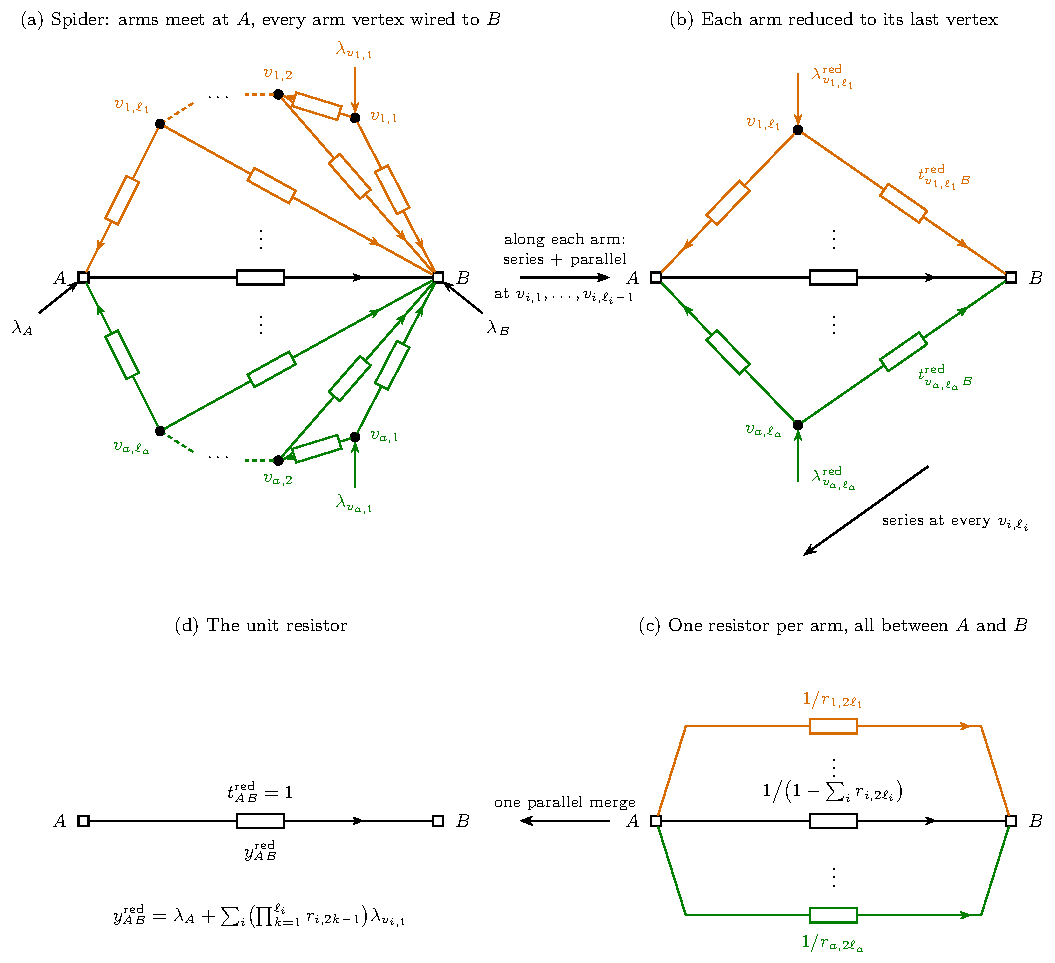
\includegraphics[width=\linewidth,height=.62\textheight,keepaspectratio]{figures/circuits/spider_order.pdf}
\caption{Order of the spider reduction. (a) The spider of \eqref{eq:1.47}: the arms, in their colours, meet at $A$, and every arm vertex is wired to $B$. (b) Series steps and parallel merges at $v_{i,1},\ldots,v_{i,\ell_i-1}$ leave on each arm its last vertex, with its reduced spoke and reduced source. (c) The series step at every $v_{i,\ell_i}$ leaves one resistor per arm between $A$ and $B$, in parallel with the original $AB$. (d) One parallel merge gives the unit resistor carrying $y^{\mathrm{red}}_{AB}$ of \eqref{eq:spider-reduced}.}
\label{fig:B-spider-order}
\end{figure}

\par\noindent\begin{minipage}{\linewidth}
On arm $i$, the edges are oriented from $v_{i,j}$ towards
$v_{i,j+1}$ and $B$, with $v_{i,\ell_i+1}=A$. Only $v_{i,1}$
carries an arm source. The dimensionless spider coordinates $r_{i,j}$
in \eqref{eq:spiderdomain} play the same role as the fan coordinates
$r_j$ in \eqref{eq:1.36}: they parameterize the original edge Schwinger times by
\begin{equation}\label{eq:1.49}
\begin{aligned}
t_{v_{i,j}v_{i,j+1}}
&=\frac{(1-r_{i,2j-1})\prod_{k=j+1}^{\ell_i}r_{i,2k-1}}
{r_{i,2\ell_i}\prod_{k=j}^{\ell_i-1}r_{i,2k}},\\
t_{v_{i,1}B}
&=\frac{\prod_{k=1}^{\ell_i}r_{i,2k-1}}
{r_{i,2\ell_i}\prod_{k=1}^{\ell_i-1}r_{i,2k}},\\
t_{v_{i,j}B}
&=\frac{\prod_{k=j}^{\ell_i}r_{i,2k-1}}
{(1-r_{i,2j-2})r_{i,2\ell_i}\prod_{k=j}^{\ell_i-1}r_{i,2k}}\quad(j\ge2),\\
t_{AB}&=\frac1{1-\sum_i r_{i,2\ell_i}}.
\end{aligned}
\end{equation}
The odd coordinate $r_{i,2j-1}$ is the fraction of the reduced source
passed to the next arm vertex. For $j<\ell_i$, the even coordinate
$r_{i,2j}$ is the fraction of the next reduced spoke current carried
by the new series edge. Figure~\ref{fig:B-spider-reduction} shows
one elimination and the current split used to reverse it.
\par\smallskip
\begingroup\captionsetup{hypcap=false}\centering
\BSpiderArmStepCircuit
\captionof{figure}{Eliminating $v_{i,j}$ on a spider arm, $j<\ell_i$.
The blue resistors combine in series; their replacement is then
merged with the original spoke. The source is redistributed to
$v_{i,j+1}$ and $B$. Reversing these steps gives the three displayed
currents. The common component index $+\dot a$ is suppressed.}
\label{fig:B-spider-reduction}
\par\endgroup
\end{minipage}
\paragraph{Eliminating $v_{i,1}$.}
For $\ell_i\ge2$, eliminating $v_{i,1}$ gives
\begin{equation}\label{eq:spider-first-series}
\begin{aligned}
t_{v_{i,1}v_{i,2}}+t_{v_{i,1}B}
&=\frac{\prod_{k=2}^{\ell_i}r_{i,2k-1}}
{r_{i,2\ell_i}\prod_{k=1}^{\ell_i-1}r_{i,2k}},\\
\frac{t_{v_{i,1}B}}{t_{v_{i,1}v_{i,2}}+t_{v_{i,1}B}}
&=r_{i,1},\\
\lambda_{v_{i,2},+\dot a}^{\mathrm{red}}
&=r_{i,1}\lambda_{v_{i,1},+\dot a},\qquad
\lambda_{B,+\dot a}^{\mathrm{red}}
=\lambda_{B,+\dot a}+(1-r_{i,1})\lambda_{v_{i,1},+\dot a}.
\end{aligned}
\end{equation}
Merging the new edge with the original spoke $v_{i,2}B$ gives
\begin{equation}\label{eq:spider-first-merge}
\begin{aligned}
t_{v_{i,2}B}^{\mathrm{red}}
&=\left[\frac1{t_{v_{i,1}v_{i,2}}+t_{v_{i,1}B}}
+\frac1{t_{v_{i,2}B}}\right]^{-1}\\
&=\left[(r_{i,2}+1-r_{i,2})
\frac{r_{i,2\ell_i}\prod_{k=2}^{\ell_i-1}r_{i,2k}}
{\prod_{k=2}^{\ell_i}r_{i,2k-1}}\right]^{-1}
=\frac{\prod_{k=2}^{\ell_i}r_{i,2k-1}}
{r_{i,2\ell_i}\prod_{k=2}^{\ell_i-1}r_{i,2k}},\\
\frac{t_{v_{i,2}B}^{\mathrm{red}}}
{t_{v_{i,1}v_{i,2}}+t_{v_{i,1}B}}&=r_{i,2}.
\end{aligned}
\end{equation}
The original currents can therefore be recovered from the reduced spoke:
\begin{equation}\label{eq:spider-first-current}
\begin{aligned}
y_{v_{i,1}v_{i,2},+\dot a}
&=r_{i,1}\lambda_{v_{i,1},+\dot a}
-r_{i,2}y^{\mathrm{red}}_{v_{i,2}B,+\dot a},\\
y_{v_{i,1}B,+\dot a}
&=(1-r_{i,1})\lambda_{v_{i,1},+\dot a}
+r_{i,2}y^{\mathrm{red}}_{v_{i,2}B,+\dot a},\\
y_{v_{i,2}B,+\dot a}
&=(1-r_{i,2})y^{\mathrm{red}}_{v_{i,2}B,+\dot a}.
\end{aligned}
\end{equation}

\paragraph{Eliminating $v_{i,2}$.}
For $\ell_i\ge3$, the second elimination starts with this reduced spoke:
\begin{equation}\label{eq:spider-second-reduction}
\begin{aligned}
t_{v_{i,2}v_{i,3}}+t_{v_{i,2}B}^{\mathrm{red}}
&=\frac{\prod_{k=3}^{\ell_i}r_{i,2k-1}}
{r_{i,2\ell_i}\prod_{k=2}^{\ell_i-1}r_{i,2k}},\\
t_{v_{i,3}B}^{\mathrm{red}}
&=\left[(r_{i,4}+1-r_{i,4})
\frac{r_{i,2\ell_i}\prod_{k=3}^{\ell_i-1}r_{i,2k}}
{\prod_{k=3}^{\ell_i}r_{i,2k-1}}\right]^{-1},\\
\lambda_{v_{i,3},+\dot a}^{\mathrm{red}}
&=r_{i,1}r_{i,3}\lambda_{v_{i,1},+\dot a},\\
y^{\mathrm{red}}_{v_{i,2}B,+\dot a}
&=(1-r_{i,3})r_{i,1}\lambda_{v_{i,1},+\dot a}
+r_{i,4}y^{\mathrm{red}}_{v_{i,3}B,+\dot a}.
\end{aligned}
\end{equation}
\paragraph{The general step and the final merge.}
Before eliminating $v_{i,j}$, its spoke and source are
\begin{equation}\label{eq:spider-reduced-data}
\begin{aligned}
t^{\mathrm{red}}_{v_{i,j}B}
&=\frac{\prod_{k=j}^{\ell_i}r_{i,2k-1}}
{r_{i,2\ell_i}\prod_{k=j}^{\ell_i-1}r_{i,2k}},\\
\lambda^{\mathrm{red}}_{v_{i,j},+\dot a}
&=\left(\prod_{k=1}^{j-1}r_{i,2k-1}\right)
\lambda_{v_{i,1},+\dot a}.
\end{aligned}
\end{equation}
At the last vertex, the two resistances sum to $1/r_{i,2\ell_i}$.
Each arm leaves an $AB$ branch of this resistance.
Merging these branches in parallel with the original $AB$ edge gives
\begin{equation}\label{eq:spider-final-scale}
\frac1{t_{AB}^{\mathrm{red}}}
=\frac1{t_{AB}}+\sum_i r_{i,2\ell_i}
=1-\sum_i r_{i,2\ell_i}+\sum_i r_{i,2\ell_i}=1.
\end{equation}
This is the scale choice in \eqref{eq:1.49}. Conservation at $A$
gives \eqref{eq:spider-reduced}. At $B$, the transferred sources give
\[
\lambda_{B,+\dot a}^{\mathrm{red}}
=\lambda_{B,+\dot a}
+\sum_i\left(1-\prod_{j=1}^{\ell_i}r_{i,2j-1}\right)
\lambda_{v_{i,1},+\dot a},
\qquad
 y_{AB,+\dot a}^{\mathrm{red}}=-\lambda_{B,+\dot a}^{\mathrm{red}}.
\]
\paragraph{Current reconstruction.}
Reversing the eliminations gives
\begin{equation}\label{eq:spider-reconstruction-recurrence}
\begin{aligned}
y^{\mathrm{red}}_{v_{i,\ell_i}B,+\dot a}
&=(1-r_{i,2\ell_i-1})
\left(\prod_{k=1}^{\ell_i-1}r_{i,2k-1}\right)
\lambda_{v_{i,1},+\dot a}
+r_{i,2\ell_i}y^{\mathrm{red}}_{AB,+\dot a},\\
y^{\mathrm{red}}_{v_{i,j}B,+\dot a}
&=(1-r_{i,2j-1})\lambda^{\mathrm{red}}_{v_{i,j},+\dot a}
+r_{i,2j}y^{\mathrm{red}}_{v_{i,j+1}B,+\dot a}\quad(j<\ell_i).
\end{aligned}
\end{equation}
Expanding the finite recurrence yields
\begin{equation}\label{eq:1.50}
\begin{aligned}
y^{\mathrm{red}}_{v_{i,j}B,+\dot a}
={}&\sum_{r=j}^{\ell_i}
\left(\prod_{k=j}^{r-1}r_{i,2k}\right)(1-r_{i,2r-1})
\left(\prod_{k=1}^{r-1}r_{i,2k-1}\right)\lambda_{v_{i,1},+\dot a}\\
&+\left(\prod_{k=j}^{\ell_i-1}r_{i,2k}\right)r_{i,2\ell_i}\,
y^{\mathrm{red}}_{AB,+\dot a}.
\end{aligned}
\end{equation}
Finally, restore each original spoke and use conservation at its arm vertex:
\begin{equation}\label{eq:1.51}
\begin{aligned}
y_{v_{i,j}v_{i,j+1},+\dot a}
&=\lambda^{\mathrm{red}}_{v_{i,j},+\dot a}
-y^{\mathrm{red}}_{v_{i,j}B,+\dot a},\\
y_{v_{i,1}B,+\dot a}&=y^{\mathrm{red}}_{v_{i,1}B,+\dot a},\\
y_{v_{i,j}B,+\dot a}
&=(1-r_{i,2j-2})y^{\mathrm{red}}_{v_{i,j}B,+\dot a}\quad(j\ge2),\\
y_{AB,+\dot a}
&=\left(1-\sum_i r_{i,2\ell_i}\right)y^{\mathrm{red}}_{AB,+\dot a}.
\end{aligned}
\end{equation}
Substituting \eqref{eq:1.50} in \eqref{eq:1.51} and telescoping gives the arm currents
\begin{equation}\label{eq:spider-arm-current}
\begin{aligned}
y_{v_{i,j}v_{i,j+1},+\dot a}
={}&\sum_{s=j}^{\ell_i-1}
\left(\prod_{k=1}^{s}r_{i,2k-1}\right)
\left(\prod_{k=j}^{s-1}r_{i,2k}\right)(1-r_{i,2s})\,
\lambda_{v_{i,1},+\dot a}\\
&+\left(\prod_{k=1}^{\ell_i}r_{i,2k-1}\right)
\left(\prod_{k=j}^{\ell_i-1}r_{i,2k}\right)
\lambda_{v_{i,1},+\dot a}
-\left(\prod_{k=j}^{\ell_i}r_{i,2k}\right)
y^{\mathrm{red}}_{AB,+\dot a}.
\end{aligned}
\end{equation}
Take the spokes and $AB$ as spanning tree. Conservation at every vertex gives, for arbitrary displacements,
\begin{equation}\label{eq:spider-loop-split}
\begin{aligned}
\sum_e y_{e,+\dot a}z_e^{+\dot a}
={}&\lambda_{A,+\dot a}z_{AB}^{+\dot a}
+\sum_i\lambda_{v_{i,1},+\dot a}z_{v_{i,1}B}^{+\dot a}\\
&+\sum_{i=1}^a\sum_{j=1}^{\ell_i}
y_{v_{i,j}v_{i,j+1},+\dot a}
(z_{v_{i,j}v_{i,j+1}}+z_{v_{i,j+1}B}-z_{v_{i,j}B})^{+\dot a},
\qquad v_{i,\ell_i+1}=A.
\end{aligned}
\end{equation}
In \eqref{eq:spider-full-taylor}, $p_{ijs}$ counts the $s$th $\lambda_{v_{i,1}}$ term of \eqref{eq:spider-arm-current}, the term $s=\ell_i$ included; $q_{ijA}$ and $q_{ijk}$ count the terms $\lambda_A$ and $\bigl(\prod_{h=1}^{\ell_k}r_{k,2h-1}\bigr)\lambda_{v_{k,1}}$ of $y^{\mathrm{red}}_{AB}$ in its last term; $m_{iA}$ and $m_{ik}$ count the same terms in the prefactor $[\lambda_{v_{i,1}}y^{\mathrm{red}}_{AB}]^{\ell_i}$. The exponents in \eqref{eq:spider-moments} are then
\begin{equation}\label{eq:spider-taylor-exponents}
\begin{gathered}
\kappa_{i,2t-1}=M_i+\sum_{s=t}^{\ell_i}\sum_{j=1}^{s}p_{ijs},\qquad
\kappa_{i,2t}=\sum_{j=1}^{t}\left[q_{ij}+\sum_{s=t+1}^{\ell_i}p_{ijs}\right]\ (t<\ell_i),\\
\bar\kappa_{i,2t}=\sum_{j=1}^{t}p_{ijt},\qquad
\kappa_{i,2\ell_i}=\sum_{j=1}^{\ell_i}q_{ij}.
\end{gathered}
\end{equation}

\subsection{The spider Jacobian}\label{sec:spider-jacobian}

\paragraph{Current reconstruction and Jacobian.}
Take the spokes and $AB$ as spanning tree. The independent currents are
those of the arm resistors, $y_{v_{i,j}v_{i,j+1}}$ with
$j=1,\ldots,\ell_i$ and $v_{i,\ell_i+1}=A$: $2n$ components. Conservation
at $v_{i,j+1}$ in the reduced network gives
$y^{\mathrm{red}}_{v_{i,j+1}B}=\lambda^{\mathrm{red}}_{v_{i,j+1}}-y_{v_{i,j+1}v_{i,j+2}}$,
with $\lambda^{\mathrm{red}}_{v_{i,j+1}}=r_{i,2j-1}\lambda^{\mathrm{red}}_{v_{i,j}}$,
and \eqref{eq:spider-reconstruction-recurrence} becomes the analogue of
\eqref{eq:B-fan-reconstruction}:
\begin{equation}\label{eq:spider-chord-recurrence}
\begin{aligned}
y_{v_{i,\ell_i}A,+\dot a}
&=r_{i,2\ell_i-1}\lambda^{\mathrm{red}}_{v_{i,\ell_i},+\dot a}
 -r_{i,2\ell_i}y^{\mathrm{red}}_{AB,+\dot a},\\
y_{v_{i,j}v_{i,j+1},+\dot a}
&=r_{i,2j-1}(1-r_{i,2j})\lambda^{\mathrm{red}}_{v_{i,j},+\dot a}
 +r_{i,2j}\,y_{v_{i,j+1}v_{i,j+2},+\dot a}\qquad(j<\ell_i),\\
y^{\mathrm{red}}_{AB,+\dot a}
&=\lambda_{A,+\dot a}+\sum_{k=1}^a r_{k,2\ell_k-1}\lambda^{\mathrm{red}}_{v_{k,\ell_k},+\dot a}.
\end{aligned}
\end{equation}
At fixed sources,
\begin{equation}\label{eq:spider-jacobian-rows}
\begin{aligned}
dy_{v_{i,j}v_{i,j+1},+\dot a}-r_{i,2j}\,dy_{v_{i,j+1}v_{i,j+2},+\dot a}
&=(1-r_{i,2j})\,d\bigl(r_{i,2j-1}\lambda^{\mathrm{red}}_{v_{i,j},+\dot a}\bigr)
 -y^{\mathrm{red}}_{v_{i,j+1}B,+\dot a}\,dr_{i,2j}\qquad(j<\ell_i),\\
dy_{v_{i,\ell_i}A,+\dot a}
&=\sum_{k=1}^a(\delta_{ik}-r_{i,2\ell_i})\,
 d\bigl(r_{k,2\ell_k-1}\lambda^{\mathrm{red}}_{v_{k,\ell_k},+\dot a}\bigr)
 -y^{\mathrm{red}}_{AB,+\dot a}\,dr_{i,2\ell_i}.
\end{aligned}
\end{equation}
Take the Jacobian matrix with rows the two components of the arm
currents and columns $r_{i,1},\ldots,r_{i,2\ell_i}$, both arm by arm. As
for the fan, subtract $r_{i,2j}$ times the rows of $y_{v_{i,j+1}v_{i,j+2}}$
from those of $y_{v_{i,j}v_{i,j+1}}$, $j<\ell_i$; the determinant does
not change. In the new rows of an interior resistor the coefficient of
$dr_{i,2j-1}$ is $(1-r_{i,2j})\lambda^{\mathrm{red}}_{v_{i,j}}$, that of
$dr_{i,2j}$ is $-y^{\mathrm{red}}_{v_{i,j+1}B}$, and the only other
columns are $r_{i,1},r_{i,3},\ldots,r_{i,2j-3}$ of the same arm
(Figure~\ref{fig:B-spider-jacobian-interior}).
\begin{figure}[H]
\centering
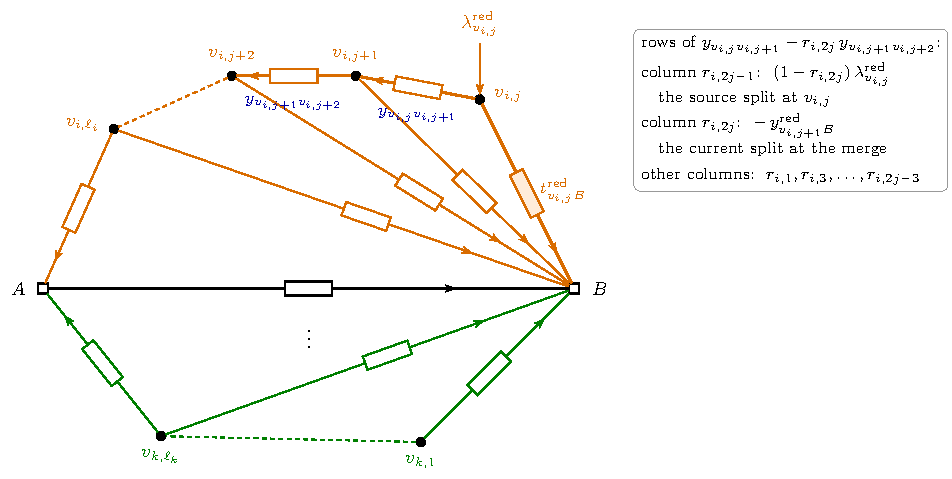
\includegraphics[width=\linewidth,height=.4\textheight,keepaspectratio]{figures/circuits/spider_jac_interior.pdf}
\caption{The rows of an interior resistor. When $v_{i,j}$ is eliminated, $v_{i,1},\ldots,v_{i,j-1}$ are already gone: $v_{i,j}$ carries the reduced source and the reduced spoke (shaded). The column of $r_{i,2j-1}$ moves the source split at $v_{i,j}$, the column of $r_{i,2j}$ the current split at the merge with the spoke of $v_{i,j+1}$.}
\label{fig:B-spider-jacobian-interior}
\end{figure}
The arms couple only through $y^{\mathrm{red}}_{AB}$, which enters the
rows of the last resistors $v_{i,\ell_i}A$
(Figure~\ref{fig:B-spider-jacobian-final}). Put the interior column
pairs $(r_{i,2j-1},r_{i,2j})$, $j<\ell_i$, first and the final pairs
$(r_{i,2\ell_i-1},r_{i,2\ell_i})$ last, with the rows in the same order.
Moving pairs of columns and pairs of rows leaves the determinant
unchanged, and the matrix is block lower triangular, with the interior
two-by-two blocks along the diagonal and one final $2a\times2a$ block.
For the three-loop spider of Figure~\ref{fig:spider-reduction}, with
$\ell_1=2$, $\ell_2=1$, $\lambda^{\mathrm{red}}_{v_{1,2}}=r_{1,1}\lambda_{v_{1,1}}$
and each entry standing for its two dotted components,
\[
\left(\begin{array}{cc|cccc}
(1-r_{1,2})\lambda_{v_{1,1}}&-y^{\mathrm{red}}_{v_{1,2}B}&0&0&0&0\\\hline
(1-r_{1,4})r_{1,3}\lambda_{v_{1,1}}&0&(1-r_{1,4})\lambda^{\mathrm{red}}_{v_{1,2}}&-y^{\mathrm{red}}_{AB}&-r_{1,4}\lambda_{v_{2,1}}&0\\
-r_{2,2}r_{1,3}\lambda_{v_{1,1}}&0&-r_{2,2}\lambda^{\mathrm{red}}_{v_{1,2}}&0&(1-r_{2,2})\lambda_{v_{2,1}}&-y^{\mathrm{red}}_{AB}
\end{array}\right),
\]
with rows $y_{v_{1,1}v_{1,2}}-r_{1,2}y_{v_{1,2}A}$, $y_{v_{1,2}A}$,
$y_{v_{2,1}A}$ and columns $r_{1,1},r_{1,2}\,|\,r_{1,3},r_{1,4},r_{2,1},r_{2,2}$.
\begin{figure}[H]
\centering
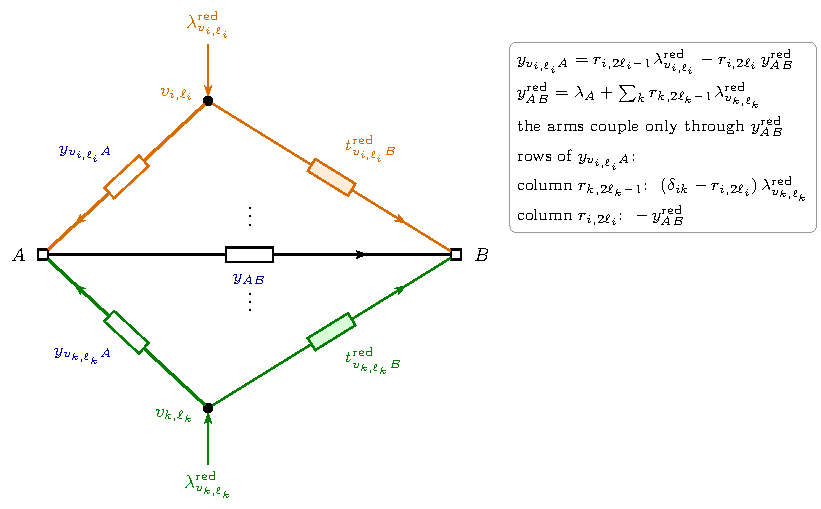
\includegraphics[width=\linewidth,height=.4\textheight,keepaspectratio]{figures/circuits/spider_jac_final.pdf}
\caption{The rows of the final block, at the end of the iteration: every arm is reduced to its last vertex, as in Figure~\ref{fig:B-spider-order}(b). The last arm resistors $v_{i,\ell_i}A$ all carry the common current $y^{\mathrm{red}}_{AB}$ with their final shares, so the final block is that of a book.}
\label{fig:B-spider-jacobian-final}
\end{figure}
A diagonal block has its two coefficient vectors $u,w$ as columns, and
its determinant is their pairing $u_{+\dot a}w_+{}^{\dot a}$. With
$y^{\mathrm{red}}_{v_{i,j+1}B}=r_{i,2j-1}\lambda^{\mathrm{red}}_{v_{i,j}}-y_{v_{i,j+1}v_{i,j+2}}$
and $\lambda^{\mathrm{red}}_{v_{i,j},+\dot a}\lambda_{v_{i,j},+}^{\mathrm{red}\,\dot a}=0$,
an interior block is
\begin{equation}\label{eq:spider-jacobian-blocks}
\underbrace{(1-r_{i,2j})\lambda^{\mathrm{red}}_{v_{i,j},+\dot a}
\bigl(-y^{\mathrm{red}\,\dot a}_{v_{i,j+1}B,+}\bigr)}_{\text{columns }r_{i,2j-1},\,r_{i,2j}}
=(1-r_{i,2j})\lambda^{\mathrm{red}}_{v_{i,j},+\dot a}
y_{v_{i,j+1}v_{i,j+2},+}{}^{\dot a}\qquad(j<\ell_i),
\end{equation}
the fan block \eqref{eq:B-fan-jacobian-blocks} with $r_{2i}$ replaced by
$1-r_{i,2j}$ and no source at $v_{i,j+1}$. In the final block, the
column of $r_{k,2\ell_k}$ is $-y^{\mathrm{red}}_{AB}$ in the rows of arm
$k$ and zero elsewhere, and that of $r_{k,2\ell_k-1}$ is
$(\delta_{ik}-r_{i,2\ell_i})\lambda^{\mathrm{red}}_{v_{k,\ell_k}}$ in the
rows of arm $i$. Every even column lies along $y^{\mathrm{red}}_{AB}$, so
each odd column contributes its pairing with $-y^{\mathrm{red}}_{AB}$,
and the matrix $(\delta_{ik}-r_{i,2\ell_i})$, the identity minus a
matrix of rank one, has determinant $1-\sum_ir_{i,2\ell_i}$:
\begin{equation}\label{eq:spider-final-block}
\det\bigl[(\delta_{ik}-r_{i,2\ell_i})\,
\lambda^{\mathrm{red}}_{v_{k,\ell_k},+\dot a}
\bigl(-y^{\mathrm{red}\,\dot a}_{AB,+}\bigr)\bigr]_{i,k=1}^a
=(-1)^a\Bigl(1-\sum_ir_{i,2\ell_i}\Bigr)
\prod_{k=1}^a\lambda^{\mathrm{red}}_{v_{k,\ell_k},+\dot a}
y^{\mathrm{red}\,\dot a}_{AB,+}.
\end{equation}
For $\ell_i=1$ this is the book determinant of
Section~\ref{sec:book-jacobian}.

The arm currents \eqref{eq:spider-arm-current} carry
$y^{\mathrm{red}}_{AB}$ only in their last term, and their other terms
are proportional to $\lambda_{v_{i,1}}$. Hence
\[
\lambda^{\mathrm{red}}_{v_{i,j},+\dot a}y_{v_{i,j+1}v_{i,j+2},+}{}^{\dot a}
=-\Bigl(\prod_{h=1}^{j-1}r_{i,2h-1}\Bigr)
\Bigl(\prod_{m=j+1}^{\ell_i}r_{i,2m}\Bigr)
\lambda_{v_{i,1},+\dot a}y^{\mathrm{red}\,\dot a}_{AB,+},
\]
\[
\lambda^{\mathrm{red}}_{v_{i,\ell_i},+\dot a}y^{\mathrm{red}\,\dot a}_{AB,+}
=\Bigl(\prod_{h=1}^{\ell_i-1}r_{i,2h-1}\Bigr)
\lambda_{v_{i,1},+\dot a}y^{\mathrm{red}\,\dot a}_{AB,+}.
\]
In the product of the blocks of arm $i$, $r_{i,2h-1}$ occurs $\ell_i-h$
times, $r_{i,2m}$ occurs $m-1$ times and $1-r_{i,2j}$ once. The
$n-a$ interior blocks and \eqref{eq:spider-final-block} carry the sign
$(-1)^n$, which cancels against the $n$ minus signs of the chord
two-forms:
\begin{equation}\label{eq:1.54}
\begin{aligned}
&\bigwedge_{i=1}^a\bigwedge_{j=1}^{\ell_i}
\bigl(-dy_{v_{i,j}v_{i,j+1},+\dot+}\wedge dy_{v_{i,j}v_{i,j+1},+\dot-}\bigr)\\
&\quad=\Bigl(1-\sum_ir_{i,2\ell_i}\Bigr)
\prod_{i=1}^a\Bigl\{r_{i,2\ell_i}^{\ell_i-1}
\prod_{j=1}^{\ell_i-1}r_{i,2j-1}^{\ell_i-j}r_{i,2j}^{j-1}(1-r_{i,2j})
\bigl[\lambda_{v_{i,1},+\dot a}y^{\mathrm{red}}_{AB,+}{}^{\dot a}\bigr]^{\ell_i}\Bigr\}
\bigwedge_{i=1}^a\bigwedge_{j=1}^{\ell_i}(dr_{i,2j-1}\wedge dr_{i,2j}).
\end{aligned}
\end{equation}

\paragraph{The complete spider kernel.}
Together with the displacement exponential, \eqref{eq:1.54} gives, for
the source assignment \eqref{eq:1.47} and arbitrary positive arm lengths
$\ell_1+\cdots+\ell_a=n$,
\begin{equation}\label{eq:B-spider-full-kernel}
\begin{aligned}
\mathcal I_\Gamma^{\mathrm{raw\ cut}}(\lambda;z)
={}&\int_{\substack{0<r_{i,j}<1\ (j<2\ell_i)\\
 r_{i,2\ell_i}>0,\ \sum_i r_{i,2\ell_i}<1}}
 \prod_{i=1}^a\prod_{j=1}^{2\ell_i}dr_{i,j}\,
 \left(1-\sum_i r_{i,2\ell_i}\right)\\
&\times\prod_{i=1}^a\left\{
 r_{i,2\ell_i}^{\ell_i-1}
 \prod_{j=1}^{\ell_i-1}
 r_{i,2j-1}^{\ell_i-j}r_{i,2j}^{j-1}(1-r_{i,2j})
 \left[\lambda_{v_{i,1},+\dot a}
 y^{\mathrm{red}}_{AB,+}{}^{\dot a}\right]^{\ell_i}
 \right\}\\
&\times\exp\!\Bigg[-\sum_{i=1}^a\sum_{j=1}^{\ell_i}
 \left(y_{v_{i,j}v_{i,j+1},+\dot a}(r)
 z_{v_{i,j}v_{i,j+1}}^{+\dot a}
 +y_{v_{i,j}B,+\dot a}(r)z_{v_{i,j}B}^{+\dot a}\right)\\
&\hspace{49mm}
 -\left(1-\sum_i r_{i,2\ell_i}\right)
 y^{\mathrm{red}}_{AB,+\dot a}z_{AB}^{+\dot a}\Bigg].
\end{aligned}
\end{equation}
The reduced current is \eqref{eq:spider-reduced};
\eqref{eq:1.50}--\eqref{eq:1.51} give every original edge current
as a polynomial in the displayed integration coordinates.
This is \eqref{eq:1.53}, with the displacement of each edge retained.

\FloatBarrier
\Needspace{.96\textheight}
\subsection{The book Jacobian}\label{sec:book-jacobian}

\par\noindent\begin{minipage}{\linewidth}
The book is the spider with $\ell_i=1$ for every arm.
Set $A=n+1$, $B=n+2$, $r_{2i-1}=r_{i,1}$ and $r_{2i}=r_{i,2}$.
Figure~\ref{fig:B-book-circuit} follows the leaf eliminations and
the final parallel merge. The original edge resistances are
\begin{equation}\label{eq:book-edge-times}
t_{i,n+1}=\frac{1-r_{2i-1}}{r_{2i}},\qquad
t_{i,n+2}=\frac{r_{2i-1}}{r_{2i}},\qquad
t_{n+1,n+2}=\frac1{1-\sum_i r_{2i}}.
\end{equation}
\par\smallskip
\begingroup\captionsetup{hypcap=false}\centering
\BBookCurrentReductionCircuit
\captionof{figure}{Reducing an $n$-loop book to a unit resistor.
Each leaf contributes one parallel branch of resistance $1/r_{2i}$;
the original common edge supplies the remaining conductance.
The representative leaves show the same reduction for every $i$.
Both endpoint sources are transferred as displayed. Blue arrows
orient the currents; the common component index $+\dot a$ is suppressed.}
\label{fig:B-book-circuit}
\par\endgroup
Conservation on the reduced edge and the parallel current fractions give
\begin{equation}\label{eq:B-book-reduced-current}
\begin{aligned}
y^{\mathrm{red}}_{n+1,n+2,+\dot a}
&=\lambda_{n+1,+\dot a}+\sum_{j=1}^n r_{2j-1}\lambda_{j,+\dot a},\\
y_{i,n+1,+\dot a}
&=r_{2i-1}\lambda_{i,+\dot a}
-r_{2i}y^{\mathrm{red}}_{n+1,n+2,+\dot a},\\
y_{i,n+2,+\dot a}
&=(1-r_{2i-1})\lambda_{i,+\dot a}
+r_{2i}y^{\mathrm{red}}_{n+1,n+2,+\dot a},\\
y_{n+1,n+2,+\dot a}
&=\left(1-\sum_i r_{2i}\right)y^{\mathrm{red}}_{n+1,n+2,+\dot a}.
\end{aligned}
\end{equation}
\end{minipage}
At fixed sources, differentiate $y_{i,n+1}$:

\begin{equation}\label{eq:book-current-derivative}
dy_{i,n+1,+\dot a}
=\sum_j(\delta_{ij}-r_{2i})\lambda_{j,+\dot a}\,dr_{2j-1}
-y^{\mathrm{red}}_{n+1,n+2,+\dot a}\,dr_{2i}.
\end{equation}
Every even-coordinate column lies along $y^{\mathrm{red}}_{n+1,n+2}$. In the determinant,
the remaining column in each two-component block contributes its
antisymmetric contraction with $y^{\mathrm{red}}_{n+1,n+2}$. Therefore
\begin{equation}\label{eq:book-current-determinant}
\begin{aligned}
\det\!\left((\delta_{ij}-r_{2i})
\lambda_{j,+\dot a}y^{\mathrm{red}}_{n+1,n+2,+}{}^{\dot a}\right)
&=\det\!\left(\delta_{ij}-r_{2i}\right)
\prod_j\lambda_{j,+\dot a_j}y^{\mathrm{red}}_{n+1,n+2,+}{}^{\dot a_j}\\
&=\left(1-\sum_i r_{2i}\right)
\prod_j\lambda_{j,+\dot a_j}y^{\mathrm{red}}_{n+1,n+2,+}{}^{\dot a_j}.
\end{aligned}
\end{equation}
The matrix $(r_{2i})_{ij}$ has identical columns, so its minors of
order two and higher vanish; the determinant retains the constant
term and minus its trace. Each even-coordinate column also contributes
a minus sign from \eqref{eq:book-current-derivative}. Thus
\[
\begin{aligned}
&\det\frac{\partial(y_{1,n+1,+\dot+},y_{1,n+1,+\dot-},\ldots,
 y_{n,n+1,+\dot+},y_{n,n+1,+\dot-})}
 {\partial(r_1,r_2,\ldots,r_{2n})}\\
&\qquad=(-1)^n\left(1-\sum_i r_{2i}\right)
 \prod_{i=1}^n
 \lambda_{i,+\dot a_i}y^{\mathrm{red}}_{n+1,n+2,+}{}^{\dot a_i}.
\end{aligned}
\]
For the spanning tree consisting of $AB$ and all $iB$,
the complementary currents are $y_{i,n+1}$.
The $n$ minus signs in the ordered current form
\eqref{eq:1.67} cancel this determinant sign:

\begin{equation}\label{eq:book-oriented-measure}
\bigwedge_{i=1}^{n}
\left[-dy_{i,n+1,+\dot+}\wedge dy_{i,n+1,+\dot-}\right]
=\left(1-\sum_i r_{2i}\right)
\prod_i\left[\lambda_{i,+\dot a_i}y^{\mathrm{red}}_{n+1,n+2,+}{}^{\dot a_i}\right]
\bigwedge_{i=1}^{n}(dr_{2i-1}\wedge dr_{2i}).
\end{equation}
\paragraph{The complete book kernel.}
Inserting these currents in the displacement exponential gives,
for every $n\ge1$,
\begin{equation}\label{eq:B-book-full-kernel}
\begin{aligned}
\mathcal I_\Gamma^{\mathrm{raw\ cut}}(\lambda;z)
={}&\int_{\substack{0<r_{2i-1}<1\\r_{2i}>0,\ \sum_i r_{2i}<1}}
 \prod_{i=1}^n(dr_{2i-1}\,dr_{2i})\\
&\times\left(1-\sum_i r_{2i}\right)
 \prod_{i=1}^n\left[
 \lambda_{i,+\dot a_i}y^{\mathrm{red}}_{n+1,n+2,+}{}^{\dot a_i}
 \right]\\
&\times\exp\!\Bigg[
 -\sum_{i=1}^n
 \left(r_{2i-1}\lambda_{i,+\dot a}
       -r_{2i}y^{\mathrm{red}}_{n+1,n+2,+\dot a}\right)
 z_{i,n+1}^{+\dot a}\\
&\hspace{22mm}
 -\sum_{i=1}^n
 \left((1-r_{2i-1})\lambda_{i,+\dot a}
       +r_{2i}y^{\mathrm{red}}_{n+1,n+2,+\dot a}\right)
 z_{i,n+2}^{+\dot a}\\
&\hspace{22mm}
 -\left(1-\sum_i r_{2i}\right)
 y^{\mathrm{red}}_{n+1,n+2,+\dot a}
 z_{n+1,n+2}^{+\dot a}\Bigg].
\end{aligned}
\end{equation}
Here $y^{\mathrm{red}}_{n+1,n+2}$ is the source sum in
\eqref{eq:B-book-reduced-current}. Setting every spider arm length
to one in \eqref{eq:B-spider-full-kernel} gives this same expression.
For the marked quantum product, $z_{n+1,n+2}=0$.

\FloatBarrier
\subsection{Graphs of type~I\texorpdfstring{$'$}{'}}
\label{sec:B-typeI}

A graph is of type~I$'$ \cite[Definition 4.12]{GWW} if it is built from one edge by repeatedly adding a vertex joined to the two endpoints of an existing edge. Theorem~\ref{thm:kernel-series-parallel} reverses each construction step, so such graphs are reduced to that edge by series--parallel moves alone.

\begin{proposition}[Spiders and graphs of type~I$'$]\label{prop:product-spider}
Let $\Gamma$ consist of the edge $AB$, a forest of trees $T_j$, and at most one spoke from each interaction vertex to each insertion, with $|E_j|=|T_j|+1$.
\begin{enumerate}
\item[(i)] $\Gamma$ is of type~I$'$ if and only if the two endpoints of every internal edge are joined to a common insertion.
\item[(ii)] For cubic interactions, $\Gamma$ is of type~I$'$ if and only if every tree is a path $v_{i,1}-v_{i,2}-\cdots-v_{i,\ell_i}$, an arm, all of whose vertices are joined to the same insertion, with $v_{i,1}$ the degree-two vertex and $v_{i,\ell_i}$ joined to both insertions. For $n\ge3$, $\Gamma$ is a spider (Definition~\ref{def:spiders-books}) if and only if it is of type~I$'$ and all arms with $\ell_i\ge2$ are joined to the same insertion. Its hub, joined to every other vertex, is that insertion (either insertion for a book), and the arms meet at the other one. With hub $B$, $\Gamma$ is the spider \eqref{eq:1.47} with these arms; it is a book if all $\ell_i=1$ and a fan if it has at most two arms.
\item[(iii)] For cubic interactions, every graph with $n\le2$ is a book or a fan. Graphs not of type~I$'$ first occur at $n=3$; graphs of type~I$'$ that are not spiders, and trees with a vertex of tree degree three, first occur at $n=4$.
\end{enumerate}
\end{proposition}

\begin{proof}
(i) Each construction step wires a new node by two resistors to the two ends of an existing resistor, so in a circuit of type~I$'$ with at least three nodes every resistor closes a triangle. For an internal resistor $uv$ the third node of its triangle is wired to $u$ and to $v$; an interaction node would close a loop of internal resistors in $T_j$, so the third node is $A$ or $B$. Conversely, assume the condition and induct on $n$; for $n=0$, $\Gamma$ is the marked resistor $AB$. A tree with a single node is wired to $A$ and $B$ by its two spokes, which are in series across $AB$. Otherwise let $T_j$ have $|T_j|\ge2$ nodes and $L\ge2$ end nodes. Every node of $T_j$ lies on an internal resistor and therefore has a spoke. If every end node had two spokes, $T_j$ would have $|E_j|\ge2L+(|T_j|-L)\ge|T_j|+2$ spokes; some end node therefore has exactly one spoke, to $X\in\{A,B\}$, and its neighbour in $T_j$ is also wired to $X$. In both cases the node has two resistors in series across an existing resistor, and removing it reverses one construction step.

(ii) A node of tree degree three has no spoke by \eqref{eq:product-local-spokes}, and neither has the node with two resistors when both are internal; their internal resistors violate the condition of (i). Under that condition every tree is therefore a chain, each node of tree degree two has one spoke, and the node with two resistors, $v_{i,1}$, is an end of the chain with one spoke or a single node. Along the chain from $v_{i,1}$, each internal resistor passes the insertion wired to one node on to the next, and the far end $v_{i,\ell_i}$ has two spokes. Conversely, such arms satisfy the condition of (i). For $n\ge3$, the hub of a spider is wired to $n+1\ge4$ nodes, so it is an insertion, say $B$; every internal resistor then has its ends wired to $B$, and removing $B$ leaves the arms and the resistors $v_{i,\ell_i}A$, chains meeting only at $A$: the spider \eqref{eq:1.47}. Conversely, if all arms with $\ell_i\ge2$ are wired to $B$, then $B$ is wired to every interaction node.

(iii) For $n\le2$, \eqref{eq:product-local-spokes} allows only the triangle, the two-page book, and the two-loop fans with resistors $12,1A,2A,2B,AB$ and $12,1B,2A,2B,AB$. At $n=3$ the condition of (i) fails for the circuit $12,13,2A,2B,3A,3B,AB$, whose node $1$ with two resistors has no spoke, and for $12,13,1A,2B,3A,3B,AB$ and its mirror image, whose node $2$ with two resistors and its neighbour $1$ are wired to different insertions; the remaining five circuits are the book and four fans. A circuit of type~I$'$ that is not a spider needs arms with $\ell_i\ge2$ at both insertions, hence $n\ge4$; the first is $12,1A,2A,2B,34,3B,4A,4B,AB$. A node of tree degree three needs a tree with at least four nodes, first at $n=4$; Section~\ref{sec:forest-graphs} reduces such a circuit.
\end{proof}

\begin{remark}
In a cubic product forest (Proposition~\ref{prop:product-cubic}), the vertex of degree two starts the reduction of its tree. When its two neighbours are joined, a series--parallel move (Theorem~\ref{thm:kernel-series-parallel}) removes it and passes its source on, and its neighbour in the tree, if it has one, then has degree two in turn. Along every tree this continues until the tree is gone exactly for the graphs of type~I$'$ (Proposition~\ref{prop:product-spider}). In the other graphs, which occur from three loops on, such as $12,13,2A,2B,3A,3B,AB$, star--triangle moves at the source-free vertices, each after all the vertices of its subtree, reduce each tree to its vertex of degree two (Theorems~\ref{thm:kernel-star-triangle} and~\ref{thm:kernel-two-leaves}), which is removed last.
\end{remark}

Table~\ref{tab:product-census} lists all marked graphs with cubic vertices through seven loops, enumerated by machine up to isomorphism fixing $A$ and $B$, with every statement of Propositions~\ref{prop:product-forest}, \ref{prop:product-cubic} and~\ref{prop:product-spider} checked on each graph. By Proposition~\ref{prop:product-spider}(ii), the spiders with hub $B$ are labelled by the partitions $(\ell_i)$ of $n$, so for $n\ge3$ the number of spiders, the book included, is one less than twice the number of partitions of $n$. Books occur at every order: they are the simplest graphs of the quantum product, as fans are for $Q_n$.

\begin{table}[H]
\centering
\begin{tabular}{@{}rrrrrrrrr@{}}
\toprule
$n$ & graphs & books & fans & spiders & type~I$'$, & not type~I$'$, & branching & $A\leftrightarrow B$\\
 & & & & ($\ge3$ arms) & not spiders & paths & trees & symmetric\\
\midrule
1 & 1 & 1 & 0 & 0 & 0 & 0 & 0 & 1\\
2 & 3 & 1 & 2 & 0 & 0 & 0 & 0 & 1\\
3 & 8 & 1 & 4 & 0 & 0 & 3 & 0 & 2\\
4 & 23 & 1 & 6 & 2 & 1 & 11 & 2 & 3\\
5 & 65 & 1 & 6 & 6 & 3 & 38 & 11 & 5\\
6 & 194 & 1 & 8 & 12 & 8 & 112 & 53 & 8\\
7 & 576 & 1 & 8 & 20 & 16 & 313 & 218 & 14\\
\bottomrule
\end{tabular}
\caption{Marked graphs of the quantum product with cubic vertices, up to isomorphism fixing $A$ and $B$. Fans and spiders exclude the book. A branching tree has a vertex of tree degree three; such graphs are not of type~I$'$. The last column counts the graphs invariant under $A\leftrightarrow B$.}
\label{tab:product-census}
\end{table}

\subsection{General forests}
\label{sec:B-general-forests}

This section treats the product graphs of Section~\ref{sec:forest-graphs} that spiders and books do not cover (Figure~\ref{fig:B-general-forests}): cubic forests that are not of type~I$'$, whose trees contain trivalent vertices without sources, and trees with a superpotential vertex of higher degree, which can leave a source at a trivalent vertex. In $\mathcal N=4$ Yang--Mills theory every vertex is cubic, so every graph of the quantum product is a cubic forest of Proposition~\ref{prop:product-cubic}, as in panel (a); panel (b) needs a superpotential of degree at least four.
\begin{figure}[H]
\centering
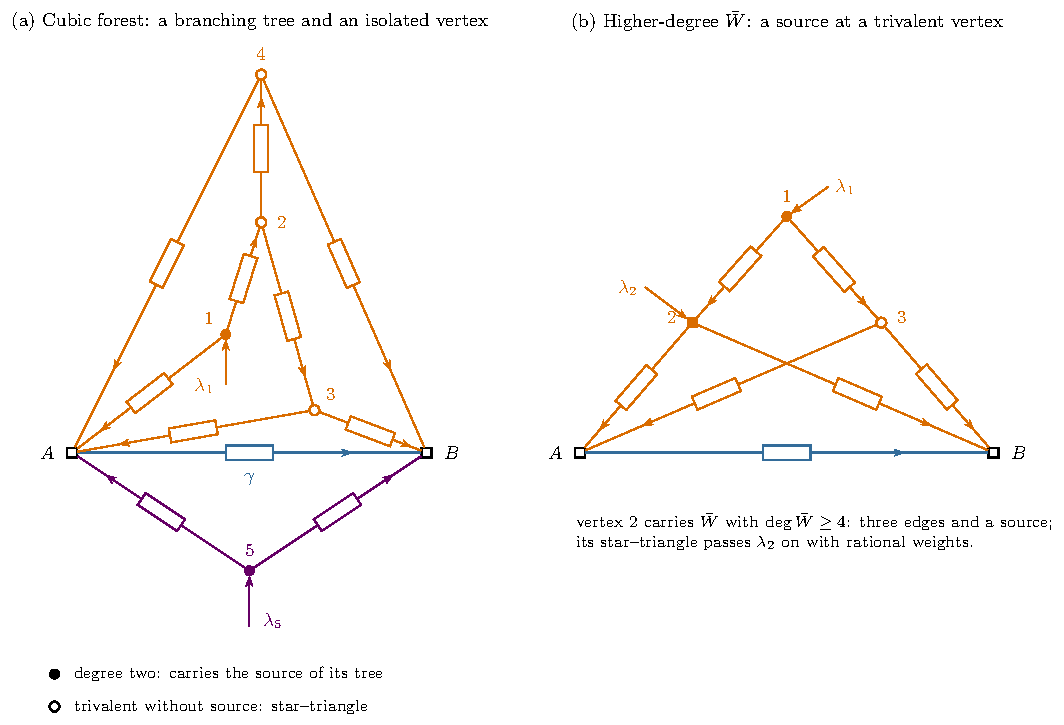
\includegraphics[width=\linewidth,height=.5\textheight,keepaspectratio]{figures/circuits/general_forests.pdf}
\caption{The graphs of this section, between the insertions $A$ and $B$ with the marked edge $\gamma$. (a) A five-loop cubic forest: the branching tree of Figure~\ref{fig:forest-star-triangle} (orange), whose source sits at its degree-two vertex $1$ and whose trivalent vertices $2,3,4$ carry none, and an isolated vertex (violet). Vertex $2$, of tree degree three, has no spoke, as \eqref{eq:product-local-spokes} requires; its tree reaches $A$ and $B$ through $1,3,4$. The source-free vertices are removed by star--triangle reductions, each after all the vertices of its subtree, and the root by a series reduction. (b) The three-loop graph $12,13,2A,2B,3A,3B,AB$ of Section~\ref{sec:forest-graphs} with a superpotential vertex $2$ (square) of degree at least four: it uses three of its fields on edges and keeps a source, so its star--triangle reduction is sourced.}
\label{fig:B-general-forests}
\end{figure}
The forests of Section~\ref{sec:forest-graphs} contain trivalent interaction vertices, which are eliminated by star--triangle reductions; with Feynman parameters as resistances, this move also appears in \cite[Section III]{PSS}, and as a change of Schwinger variables in \cite[Section 2.4.5, Lemma 2.4.23]{Panzer}. When the eliminated vertex carries no source, the reconstructed currents are linear in the reduced currents, and the currents remain polynomial in the reduction coordinates; a source at a trivalent vertex makes them rational.

\paragraph{Vertices without sources.}
At a trivalent vertex $v$ with zero source, star--triangle reduction (Figure~\ref{fig:network-moves}) gives

\begin{equation}\label{eq:1.62}
\begin{aligned}
t_{uw}^{\mathrm{red}}
&=t_{vu}+t_{vw}+\frac{t_{vu}t_{vw}}{t_{vr}},&
t_{vu}&=\frac{t_{uw}^{\mathrm{red}}t_{ur}^{\mathrm{red}}}
{t_{uw}^{\mathrm{red}}+t_{ur}^{\mathrm{red}}+t_{wr}^{\mathrm{red}}},\\
y_{vu,+\dot a}&=-y_{uw,+\dot a}^{\mathrm{red}}-y_{ur,+\dot a}^{\mathrm{red}},\\
y_{vw,+\dot a}&=y_{uw,+\dot a}^{\mathrm{red}}-y_{wr,+\dot a}^{\mathrm{red}},\\
y_{vr,+\dot a}&=y_{ur,+\dot a}^{\mathrm{red}}+y_{wr,+\dot a}^{\mathrm{red}}.
\end{aligned}
\end{equation}
\begin{figure}[H]
\centering
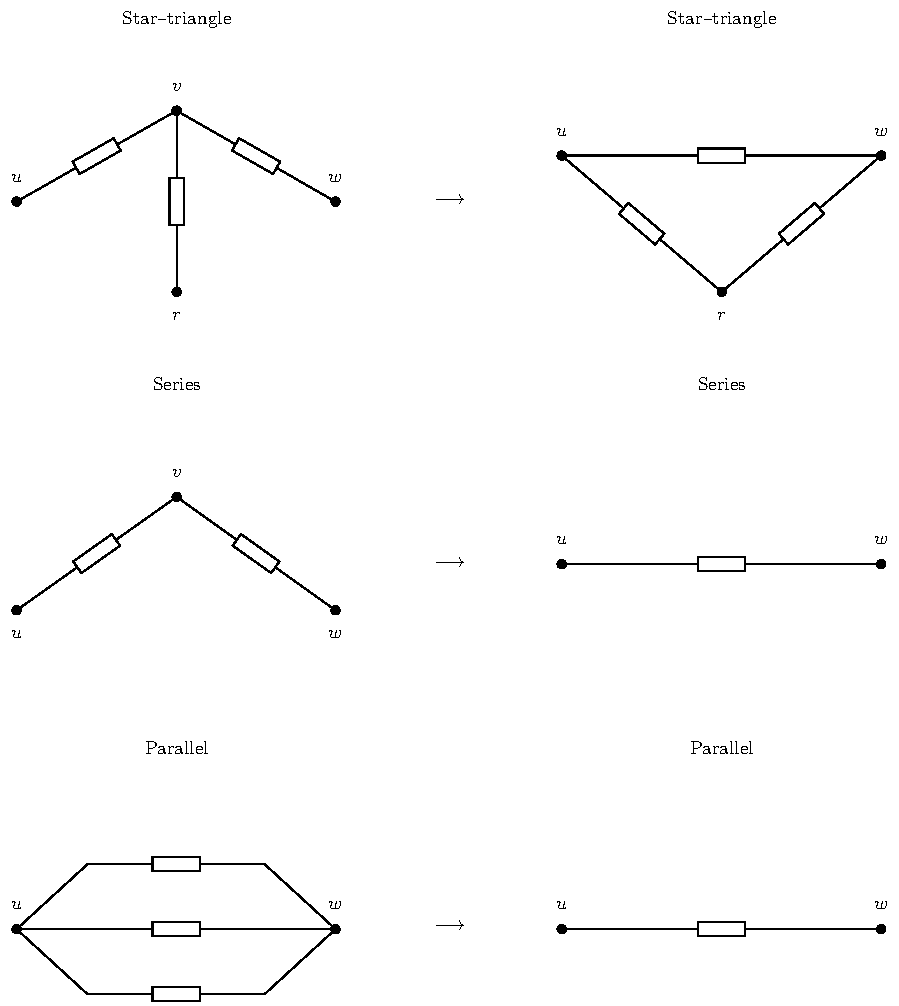
\includegraphics[width=0.78\linewidth,height=.70\textheight,keepaspectratio]{figures/circuits/network_moves.pdf}
\caption{Star--triangle, series and parallel reductions of the circuit. Every edge carries a resistor.}
\label{fig:network-moves}
\end{figure}

\paragraph{Order of the reduction.}
The trees meet only at $A$ and $B$ and are reduced one at a time
(Figure~\ref{fig:B-forest-order}). In each tree the source-free
trivalent vertices are removed by star--triangle reductions, each after all
the vertices of its subtree: such a vertex $v$, with tree neighbour $u$ towards the root, then has the neighbours $u,A,B$,
and the triangle $uA,uB,AB$ that replaces it merges in parallel with the
resistors already there. A vertex whose subtrees are gone becomes a leaf
in turn, and the tree shrinks to its root, the degree-two vertex with
the source, joined to $A$ and $B$. A series reduction at every root
leaves one resistor per tree between $A$ and $B$, and one parallel
merge with $AB$ leaves the unit resistor, as for spiders
(Figure~\ref{fig:B-spider-order}). In kernel form, a leaf whose tree neighbour keeps a spoke is removed by Theorem~\ref{thm:kernel-star-triangle}, two leaves at a vertex without spokes by Theorem~\ref{thm:kernel-two-leaves}, and every root by Theorem~\ref{thm:kernel-series-parallel}, each step integrating the kernel of the smaller circuit.
\begin{figure}[H]
\centering
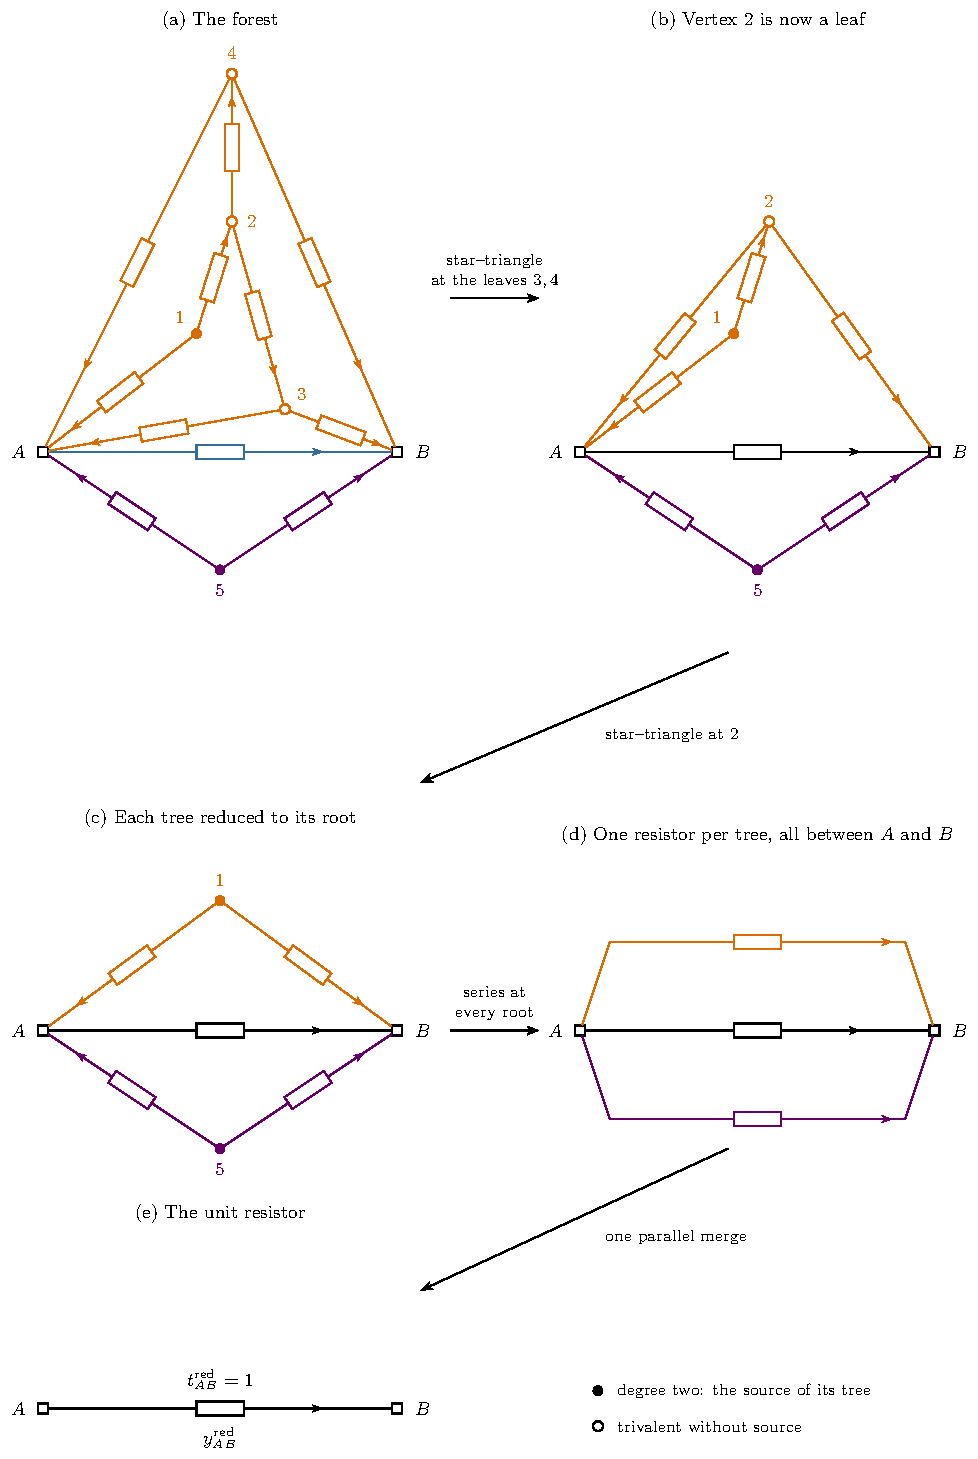
\includegraphics[width=.9\linewidth,height=.72\textheight,keepaspectratio]{figures/circuits/forest_order.pdf}
\caption{Order of the reduction of a cubic forest, for the forest of Figure~\ref{fig:B-general-forests}(a). (a)$\to$(b) Star--triangle reductions at the source-free leaves $3,4$; the new edges $2A,2B$ merge with each other and the new edges $AB$ with the marked edge, drawn black from (b) on. (b)$\to$(c) Vertex $2$ is now a source-free leaf with neighbours $1,A,B$; its star--triangle reduction leaves the root $1$ joined to $A$ and $B$, like the isolated vertex $5$. (c)$\to$(d) A series reduction at every root leaves one resistor per tree. (d)$\to$(e) One parallel merge gives the unit resistor.}
\label{fig:B-forest-order}
\end{figure}
\begin{figure}[H]
\centering
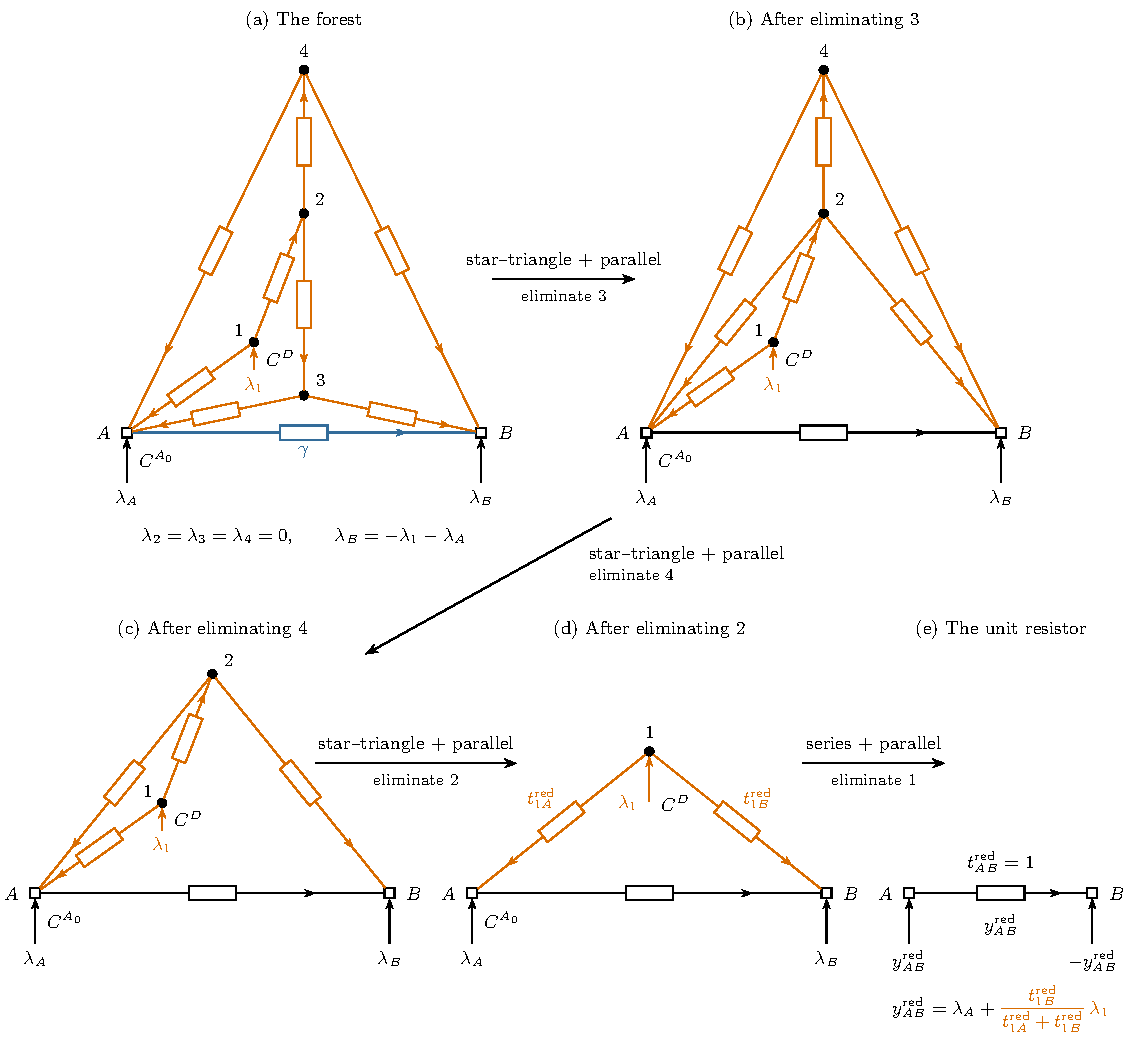
\includegraphics[width=0.98\linewidth,height=.70\textheight,keepaspectratio]{figures/circuits/forest_star_triangle_v3.pdf}
\caption{Reduction of a four-loop branching product forest, with tree edges $12,23,24$, spokes $1A,3A,3B,4A,4B$ and the marked edge $AB$ in blue. Star--triangle reductions at the source-free leaves $3$ and $4$ replace them by triangles on $2,A,B$, whose edges merge in parallel with existing edges; vertex $2$ is then a source-free leaf with neighbours $1,A,B$ and is replaced by a triangle on $1,A,B$. The root $1$, carrying $\lambda_1$, is removed last by a series reduction and a parallel merge with $AB$. After the first merge the edge $AB$ is drawn black.}
\label{fig:forest-star-triangle}
\end{figure}


Each parallel merge supplies a simplex of fractions and each series reduction an interval. Together they give $2n$ coordinates. Fix the final edge Schwinger time to one. For cubic forests, reversing the reductions produces polynomial currents and hence a polynomial pullback of

\begin{equation}\label{eq:1.67}
(-1)^n\exp\!\left[-\sum_{e\in\Gamma_1}y_{e,+\dot a}z_e^{+\dot a}\right]\bigwedge_{e\notin T}\left(dy_{e,+\dot+}\wedge dy_{e,+\dot-}\right).
\end{equation}

At any fixed input-jet order, the coefficient is obtained by replacing the exponential with the required product of currents and integrating monomials. For a simplex $\Delta$ with coordinates $r_j$ and $\sum_{j\in\Delta}r_j<1$,
\begin{equation}\label{eq:Dirichlet}
\int_\Delta\prod_{j\in\Delta}r_j^{m_j}\prod_{j\in\Delta}dr_j
=\frac{\prod_{j\in\Delta}m_j!}
{(\dim\Delta+\sum_{j\in\Delta}m_j)!}.
\end{equation}
Applying this identity to every simplex completes the finite evaluation.

\paragraph{Counting with a superpotential vertex.}
For a superpotential vertex of higher degree in $T_j$, $\deg_\Gamma\bar W$ counts its contractions and $\deg\bar W$ the factors of its monomial. The degree sum \eqref{eq:product-degree-sum} and the field count of \eqref{eq:1.21} become
\begin{equation}\label{eq:1.23}
\begin{aligned}
\#\{\text{degree-two cubic vertices}\}&=\underbrace{3(|T_j|-1)}_{\text{three per cubic vertex}}-\underbrace{\bigl(3|T_j|-1-\deg_\Gamma\bar W\bigr)}_{\substack{\text{their degrees,}\\\text{by \eqref{eq:product-degree-sum}}}}=\deg_\Gamma\bar W-2,\\
\#\{\text{fields surviving at }\bar W\}&=\deg\bar W-\deg_\Gamma\bar W,\\
\#\{\text{fields surviving in }T_j\}&=\underbrace{3(|T_j|-1)+\deg\bar W}_{\text{fields}}-\underbrace{(3|T_j|-1)}_{\substack{\text{contracted ends,}\\\text{\eqref{eq:product-degree-sum}}}}=\deg\bar W-2.
\end{aligned}
\end{equation}
Each resistor at the superpotential vertex beyond the second thus leaves one more cubic vertex of degree two, and with it one more source in the tree. For $\deg\bar W=2$ the tree has no source, as in the last step of the proof of Proposition~\ref{prop:product-forest}.

\paragraph{Sources at a trivalent vertex.}

If $\lambda_v\ne0$ at a trivalent vertex, set
$\Sigma=t_{uw}^{\mathrm{red}}+t_{ur}^{\mathrm{red}}+t_{wr}^{\mathrm{red}}$.
The additional source terms are

\begin{equation}\label{eq:1.78}
\begin{aligned}
\lambda_{u,+\dot a}^{\mathrm{red}}&=\lambda_{u,+\dot a}+\frac{t_{wr}^{\mathrm{red}}}{\Sigma}\lambda_{v,+\dot a},\\
\lambda_{w,+\dot a}^{\mathrm{red}}&=\lambda_{w,+\dot a}+\frac{t_{ur}^{\mathrm{red}}}{\Sigma}\lambda_{v,+\dot a},\\
\lambda_{r,+\dot a}^{\mathrm{red}}&=\lambda_{r,+\dot a}+\frac{t_{uw}^{\mathrm{red}}}{\Sigma}\lambda_{v,+\dot a},\\[2pt]
y_{vu,+\dot a}&=\frac{t_{wr}^{\mathrm{red}}}{\Sigma}\lambda_{v,+\dot a}-y_{uw,+\dot a}^{\mathrm{red}}-y_{ur,+\dot a}^{\mathrm{red}},\\
y_{vw,+\dot a}&=\frac{t_{ur}^{\mathrm{red}}}{\Sigma}\lambda_{v,+\dot a}+y_{uw,+\dot a}^{\mathrm{red}}-y_{wr,+\dot a}^{\mathrm{red}},\\
y_{vr,+\dot a}&=\frac{t_{uw}^{\mathrm{red}}}{\Sigma}\lambda_{v,+\dot a}+y_{ur,+\dot a}^{\mathrm{red}}+y_{wr,+\dot a}^{\mathrm{red}}.
\end{aligned}
\end{equation}

To evaluate the resulting rational moments, partition the positive Schwinger times into Hepp sectors, one for each ordering $t_{\sigma(1)}<\cdots<t_{\sigma(2n+1)}$. In a sector,

\begin{equation}\label{eq:1.79}
t_{\sigma(2n+1)}=1,\qquad t_{\sigma(i)}=\prod_{j=i}^{2n}s_j,\qquad0<s_j<1,\qquad\prod_{i=1}^{2n}dt_{\sigma(i)}=\prod_{j=1}^{2n}s_j^{j-1}\,d^{2n}s .
\end{equation}

After factoring the largest spanning-tree monomial (cf.\ the corner factorization in \cite[Lemma 3]{Wang}), a fixed Taylor coefficient has sector integrand
\begin{equation}\label{eq:sectorintegrand}
\frac{\sum_mc_ms^m}{(\sum_md_ms^m)^p},\qquad
p\in\mathbb Z_{>0},\qquad
d_0=1,\quad d_m\ge0,\quad\sum_md_m=M.
\end{equation}
Here $p$ is $n+2$ plus the total displacement order of the coefficient, $m$ is a multi-index, $c_m$ and $d_m$ are the numerator and denominator coefficients after collecting monomials, and $M$ is the number of spanning trees. On the cube, $1\le\sum_md_ms^m\le M$. Expanding the denominator about $(M+1)/2$ gives

\begin{equation}\label{eq:1.81}
\begin{aligned}
\int_{[0,1]^{2n}}\frac{\sum_mc_ms^m}{(\sum_md_ms^m)^p}\,d^{2n}s
={}&\left(\frac2{M+1}\right)^p
\sum_{k=0}^\infty\binom{p+k-1}{k}\\
&\times\sum_{m\ge0}
\frac{[s^m]\left[(\sum_jc_js^j)
\left(1-\frac2{M+1}\sum_jd_js^j\right)^k\right]}
{\prod_{i=1}^{2n}(m_i+1)}.
\end{aligned}
\end{equation}

\subsection{Exact jets and their cost}\label{sec:B-jets}

This subsection proves Theorem~\ref{thm:sum-jets}, with jet coefficients as defined there: coefficients of monomials in the source--source and source--displacement pairings, treated as independent symbols.

\paragraph{Graphs.} By Propositions~\ref{prop:cotangent-count} and~\ref{prop:superpotential-spider}, a graph of $Q_n$ has at most one $\bar W$ vertex. Without one it is a fan with $\lambda_2=\cdots=\lambda_n=0$ (Proposition~\ref{prop:cubicfan}); with one it is a spider with $a\le\deg\bar W-1$ arms and the sources \eqref{eq:1.47}, by \eqref{eq:1.16}. For cubic interactions, by Propositions~\ref{prop:product-forest} and~\ref{prop:product-cubic}, every graph of the quantum product is a marked cubic forest whose trees each carry one source, at the root, and whose other interaction vertices are trivalent and source-free.

\paragraph{Charts.} Each move, the series step \eqref{eq:1.64}, the parallel merge \eqref{eq:1.63} and the source-free star--triangle move \eqref{eq:1.62}, is written in both directions by positive rational maps. The reductions of Sections~\ref{sec:B-fan-reduction}--\ref{sec:B-general-forests} therefore compose to a bijection from the reduction coordinates, on their product of intervals and simplices, onto $\mathbb{RP}^{|\Gamma_1|-1}_{>0}$; each coordinate removes one resistor, so there are $|\Gamma_1|-1=2n$ of them. Reversing a parallel merge multiplies the reduced current by the fractions $r_j$, reversing a series step adds $\mp$ the reduced current to the fractions $1-r_j$, $r_j$ of the source \eqref{eq:1.64}, and reversing a source-free star--triangle move writes the star currents as sums of reduced currents with coefficients $\pm1$. Every current is therefore polynomial in the coordinates and linear in $\lambda$, and the pullback of \eqref{eq:1.67} is a polynomial density at each jet order. For fans, spiders and books the densities are \eqref{eq:1.40}, \eqref{eq:1.53} and \eqref{eq:B-book-full-kernel}.

\paragraph{Part (i).} Expanding the exponential and the source pairings multinomially and integrating each monomial by \eqref{eq:1.44} and \eqref{eq:spider-moments} gives \eqref{eq:fan-full-taylor} and \eqref{eq:spider-full-taylor}. Each term is a monomial in the source--source and source--displacement pairings times at most $m$ factors $1/k!$ from the displacements, $O(n)$ factors $\ell_i!$, $1/m_{iA}!$, $1/m_{ik}!$, and $O(n)$ ratios of factorials of integers at most $n+m+2$. Once the factorials up to $n+m+2$ are tabulated and the at most $m$ nonzero displacement integers of a term are listed, the sums in the factorial arguments are prefix sums, and a term costs $O(n+m)$ operations.

\paragraph{Part (ii).} The summation integers of \eqref{eq:fan-full-taylor} are $r_0$, $s_0$, $r_{ik}$ $(1\le i\le k\le n)$ and $s_i$, $N_\Gamma$ in number. In \eqref{eq:spider-full-taylor}, the integers $m_{iA}$, $m_{ik}$ with $m_{iA}+\sum_{k\ne i}m_{ik}=\ell_i$ take $T_\Gamma$ values, and the integers $p_{ijs}$, $q_{ijA}$, $q_{ijk}$ together with the $a+1$ exponents of the translation prefactor number at most $N_\Gamma$. The terms of total displacement degree at most $m$ therefore number at most $T_\Gamma\binom{m+N_\Gamma}{N_\Gamma}$. A jet coefficient is the sum of the terms that multiply its monomial, so this bound also counts the work for all coefficients of order at most $m$. Finally
\[
\binom{m+N_\Gamma}{N_\Gamma}\le(N_\Gamma+1)^m,\qquad
T_\Gamma\le(n+a)^{a(a-1)},\qquad
N_\Gamma=O\bigl(n^2+na\bigr),
\]
and $\binom{m+N_\Gamma}{N_\Gamma}\le(m+1)^{N_\Gamma}$, with $T_\Gamma=1$ for fans and $a\le\deg\bar W-1$ for $Q_n$. The arm lengths of a spider of $Q_n$ form a composition of $n$ into $a$ parts, $\binom{n-1}{a-1}$ of them for each $a$.

\paragraph{Part (iv).} For a fixed graph of the quantum product with cubic vertices, the density and the currents are polynomials of bounded degree in the $2n$ coordinates. The order-$m$ part of the integrand, the density times $(-\sum_ey_{e,+\dot a}z_e^{+\dot a})^m/m!$, has degree linear in $m$, hence $O(m^{2n})$ monomials in the coordinates and polynomially many in $\lambda$ and $z$; each monomial is integrated by \eqref{eq:Dirichlet}, after expanding the factors $1-\sum r$ binomially. The time is polynomial in $m$, of degree $O(n)$.

\paragraph{Part (iii): fan coefficients.} For the $n$-loop fan with $\lambda_2=\cdots=\lambda_n=0$ put
\[
\begin{gathered}
w_i=z_{i,i+1}+z_{i+1,n+2}-z_{i,n+2},\qquad
a_0=-\lambda_{1,+\dot b}z_{1,n+2}^{+\dot b},\qquad
b_0=-\lambda_{n+1,+\dot b}z_{n+1,n+2}^{+\dot b},\\
a_i=-\lambda_{1,+\dot b}w_i^{+\dot b},\qquad
b_i=\lambda_{n+1,+\dot b}w_i^{+\dot b}.
\end{gathered}
\]
These are the pairings of \eqref{eq:fan-full-taylor}, and
\begin{equation}\label{eq:B-fan-jet-basis}
\mathcal I_\Gamma^{\mathrm{raw\ cut}}(\lambda;z)\big|_{\lambda_2=\cdots=\lambda_n=0}
=(\lambda_{1,+\dot a}\lambda_{n+1,+}{}^{\dot a})^n\,e^{a_0+b_0}\sum_{R,s}c_{R,s}\prod_{i=1}^na_i^{R_i}b_i^{s_i},
\end{equation}
where $c_{R,s}$ collects the terms of \eqref{eq:fan-full-taylor} with $\sum_kr_{ik}=R_i$ and the $s_i$ given.

\begin{lemma}[Nested Beta recursion]\label{lem:fan-recursion}
Put $\alpha_j=n-j+\sum_{i\ge j}R_i$, $\beta_i=i-1+\sum_{k\le i}s_k$, $\sigma=\sum_ks_k$ and $B(x,y)=(x-1)!\,(y-1)!/(x+y-1)!$. Let $G_1(Q)=Q^{R_1}$ and, for $1\le i\le n-2$,
\[
G_{i+1}(Q)=Q^{R_{i+1}}\sum_l\frac{Q^l}{\alpha_{i+1}+l+1}\sum_{k\ge l}\bigl([Q^k]G_i\bigr)\binom klB(k-l+2,\beta_i+l+1).
\]
Then, for $n\ge2$,
\[
c_{R,s}=\frac1{\prod_iR_i!\,s_i!}\,\frac1{\alpha_1+1}\sum_l\Bigl[\sum_{k\ge l}\bigl([Q^k]G_{n-1}\bigr)\binom klB(k-l+2,\beta_{n-1}+l+1)\Bigr]\frac{(\alpha_n+l)!\,(n-1+\sigma)!}{(\alpha_n+l+n+1+\sigma)!},
\]
and $c_{R,s}=1/(R_1+s_1+2)!$ for $n=1$. Once the factorials up to $n+m+1$ are tabulated, each $c_{R,s}$ of order $m=\sum_i(R_i+s_i)$ costs $O(n(m+1)^2)$ operations.
\end{lemma}
\begin{proof}
With the spokes as spanning tree, current conservation gives
\[
-\sum_ey_{e,+\dot a}z_e^{+\dot a}=a_0+b_0-\sum_{i=1}^ny_{i,i+1,+\dot a}w_i^{+\dot a}.
\]
By \eqref{eq:1.38} at $\lambda_2=\cdots=\lambda_n=0$, $y_{i,i+1}=P_i\lambda_1-S_i\lambda_{n+1}$ with
\[
P_i=\Bigl(\prod_{j=1}^ir_{2j-1}\Bigr)Q_i,\qquad Q_n=1,\qquad Q_i=r_{2i}+(1-r_{2i})\,r_{2i+1}Q_{i+1},\qquad
S_i=r_{2n}\prod_{j=i}^{n-1}(1-r_{2j}),
\]
so the exponent is $a_0+b_0+\sum_i(P_ia_i+S_ib_i)$. With the density of \eqref{eq:1.41},
\[
c_{R,s}=\frac1{\prod_iR_i!\,s_i!}\int_{\eqref{eq:1.37}}d^{2n}r\,
\Bigl[\prod_{j=1}^{n-1}r_{2j-1}^{n-j}r_{2j}(1-r_{2j})^{j-1}\Bigr]r_{2n}^{n-1}
\prod_{i=1}^nP_i^{R_i}S_i^{s_i}.
\]
Outside the $Q_i$, $r_{2j-1}$ carries the exponent $\alpha_j$, $r_{2j}$ and $1-r_{2j}$ carry $1$ and $\beta_j$ for $j<n$, and $r_{2n}$ carries $n-1+\sigma$; $Q_i$ depends only on $r_{2i}$, $r_{2i+1}$ and $Q_{i+1}$. Integrating $r_1$ gives $1/(\alpha_1+1)$. Integrating $r_{2i}$ with $Q_i=r+(1-r)X$, $X=r_{2i+1}Q_{i+1}$,
\[
\int_0^1r(1-r)^{\beta_i}Q_i^k\,dr=\sum_l\binom klB(k-l+2,\beta_i+l+1)X^l,
\]
and integrating $r_{2i+1}$ gives $1/(\alpha_{i+1}+l+1)$; multiplying by $Q_{i+1}^{R_{i+1}}$ gives $G_{i+1}$. At the last step $X=r_{2n-1}$, and the simplex moment $\int r_{2n-1}^Ar_{2n}^B=A!\,B!/(A+B+2)!$ gives the stated sum. For $n=1$, $P_1=r_1$ and $S_1=r_2$ on the triangle, giving $1/(R_1+s_1+2)!$, in agreement with \eqref{eq:1.46}. Each $G_i$ has degree at most $\sum_iR_i\le m$, so each of the $n$ steps costs $O((m+1)^2)$ operations.
\end{proof}

The $\binom{m+2n+2}{2n+2}$ monomials of degree at most $m$ in $a_0,b_0,a_i,b_i$ index the jet coefficients of order at most $m$ in \eqref{eq:B-fan-jet-basis}, and $e^{a_0+b_0}$ contributes only $1/(r_0!\,s_0!)$. All of them therefore cost $O\bigl(n(m+1)^2\binom{m+2n+2}{2n+2}\bigr)$ operations, which proves part~(iii).

\paragraph{Complex dimension $d$.} The moves \eqref{eq:1.64}, \eqref{eq:1.63} and \eqref{eq:1.62} relate the resistances by scalar formulas and the currents componentwise with the same scalar coefficients. For a kernel on $\mathbb C^d$ given by the analogous current integral, with $d$ components per current, the arguments of the paragraph on charts and of part~(iv) apply, with $|\Gamma_1|-1$ coordinates in place of $2n$, to any network that reduces to one resistor by these moves and satisfies $|\Gamma_1|-1=d(|\Gamma_1|-|\Gamma_0|+1)$, the degree of its current form.

\subsection{Quadratic identities from short circuits}\label{sec:B-short-circuits}

The kernels \eqref{eq:operatope} satisfy one quadratic identity for every sliding network (one resistor fewer than the Laman count \eqref{eq:1.12}, with the local bounds \eqref{eq:1.11}) \cite[Section 3.2]{operatope}, \cite[Section 3.5]{higher}; it gives the quadratic identities \eqref{eq:2.46} and \eqref{eq:quadratic-two} of the brackets. Wang proved it by Stokes' theorem on the compactified space of Schwinger times \cite[Section 4.3, Theorem 7]{Wang}. Below that proof is carried out in network language: the boundary of the space of resistance ratios consists of short circuits.

\paragraph{Ray space.}
Let $\Gamma$ be connected, without self-loops, with oriented resistors $\Gamma_1=(e_1,\ldots,e_{|\Gamma_1|})$ in a fixed order; parallel resistors are allowed. The currents $y(t)$ of \eqref{eq:1.24} depend only on the resistance ratios $[t]\in\mathbb{RP}^{|\Gamma_1|-1}_{>0}$ of \eqref{eq:C-projective-times}. Orient $\mathbb{RP}^{|\Gamma_1|-1}_{>0}$ by
\begin{equation}\label{eq:sc-eta}
\eta_\Gamma=\iota_E\bigl(dt_{e_1}\wedge\cdots\wedge dt_{e_{|\Gamma_1|}}\bigr)
=\sum_{a=1}^{|\Gamma_1|}(-1)^{a-1}t_{e_a}\bigwedge_{b\ne a}dt_{e_b},
\qquad E=\sum_{e\in\Gamma_1}t_e\frac{\partial}{\partial t_e}.
\end{equation}
On the facet $t_{e_j}=\varepsilon$ of \eqref{eq:UV-boundary},
\[
\eta_\Gamma=(-1)^{j-1}\varepsilon\bigwedge_{a\ne j}dt_{e_a},
\]
a positive multiple of the facet orientation, and each ray with $\max_et_e/\min_et_e\le L/\varepsilon$ meets $\partial_{\mathrm{UV}}[\varepsilon,L]^{|\Gamma_1|}$ exactly once. At fixed resistances the currents injected at the nodes depend on the node potentials $\tfrac12\epsilon_{\dot a\dot b}x_v^{-\dot b}$ of \eqref{eq:1.8} through the conductance matrix with one node grounded, in each dotted component; with the real $x_v^-$ of \eqref{eq:C-current-delta-integral} oriented by $\bigwedge_vdx_v^{-\dot+}\wedge dx_v^{-\dot-}$ over the ungrounded nodes, this linear map has determinant $(\det\text{ of the conductance matrix})^2\allowbreak\det(\tfrac12\epsilon_{\dot a\dot b})^{|\Gamma_0|-1}>0$. The slice of $\Delta_\Gamma$ on which these injected currents equal $\lambda_v$ \eqref{eq:1.9} therefore carries the orientation $\eta_\Gamma$, and \eqref{eq:operatope} reads
\begin{equation}\label{eq:sc-kernel}
\mathcal I_\Gamma^{\mathrm{raw\ cut}}(\lambda;z)
=\int_{(\mathbb{RP}^{|\Gamma_1|-1}_{>0},\,\eta_\Gamma)}
e^{-\sum_ez_e^{+\dot a}y_{e,+\dot a}(t)}\bigwedge_{e\notin T}\bigl(-d^2y_e(t)\bigr),
\end{equation}
with $d$ acting on the ratios at fixed $\lambda$. In the simplex chart $t_{e_1}=1-\sum_{a=1}^{|\Gamma_1|-1}r_a$, $t_{e_{a+1}}=r_a$,
\[
\eta_\Gamma=\Bigl(t_{e_1}+\sum_{a=1}^{|\Gamma_1|-1}r_a\Bigr)dr_1\wedge\cdots\wedge dr_{|\Gamma_1|-1}=dr_1\wedge\cdots\wedge dr_{|\Gamma_1|-1} ;
\]
for the triangle with resistor order $(12),(13),(23)$ this is the orientation $dr_1\wedge dr_2$ of \eqref{eq:1.25} (Figure~\ref{fig:sc-ray}), and \eqref{eq:sc-kernel} reproduces \eqref{eq:1.25} and the two-loop case of \eqref{eq:1.40}.
\begin{figure}[H]
\centering
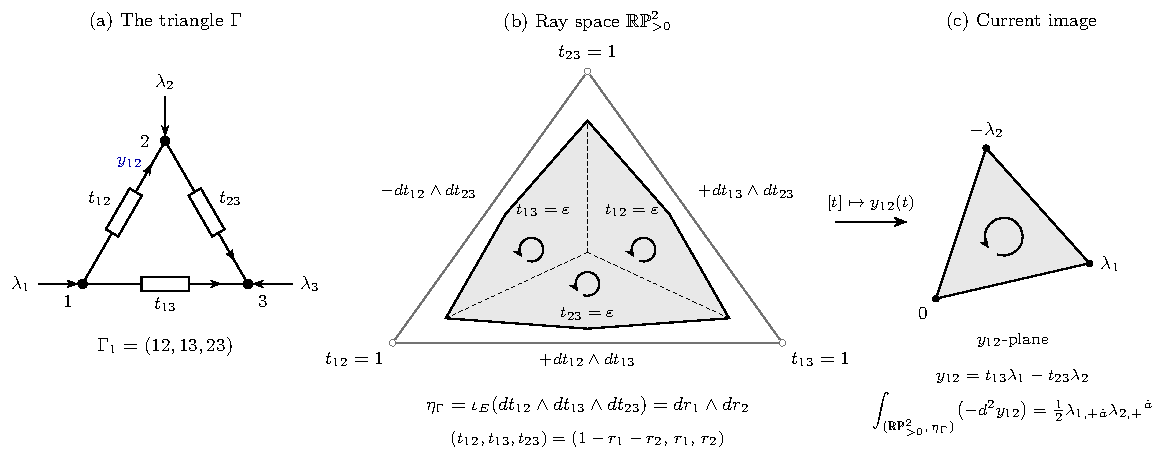
\includegraphics[width=0.98\linewidth]{figures/circuits/sc_ray.pdf}
\caption{The triangle, $\Gamma_1=(12,13,23)$. (a) Resistors $t_{12},t_{13},t_{23}$ fed by $\lambda_1,\lambda_2,\lambda_3$. (b) The ratios $[t]\in\mathbb{RP}^2_{>0}$ as the simplex $t_{12}+t_{13}+t_{23}=1$, oriented by $\eta_\Gamma=dr_1\wedge dr_2$ (circular arrows). The shaded hexagon holds the rays with $\max_et_e/\min_et_e\le L/\varepsilon$ (drawn at $L/\varepsilon=9$); the rays through the facet $t_{e_j}=\varepsilon$ of \eqref{eq:UV-boundary} are those on which $t_{e_j}$ is the smallest resistance, and there $\eta_\Gamma$ is a positive multiple of the facet orientation $(-1)^{j-1}\bigwedge_{a\ne j}dt_{e_a}$. (c) The loop current $y_{12}=t_{13}\lambda_1-t_{23}\lambda_2$ maps the simplex onto the triangle of the tree currents $y^T_{12}=0,\lambda_1,-\lambda_2$, carrying the orientation along; the swept volume is \eqref{eq:1.25} at $z=0$.}
\label{fig:sc-ray}
\end{figure}


\paragraph{Almost-Laman networks.}
A network is almost Laman if it has one resistor fewer than \eqref{eq:1.12}:
\begin{equation}\label{eq:sc-almost}
|\Gamma_1|=2|\Gamma_0|-4,\qquad
h_1(\Gamma_1)=|\Gamma_1|-|\Gamma_0|+1=|\Gamma_0|-3 ,
\end{equation}
with $h_1$ the number of independent loops. Those satisfying the local bounds \eqref{eq:1.11} are the sliding graphs of \cite[Section 3]{operatope} and the almost $2$-Laman graphs of degree one of \cite[Section 3.3]{higher}.

\begin{lemma}[Closed current form]\label{lem:sc-closed}
For an almost-Laman network the integrand of \eqref{eq:sc-kernel} is a closed form of degree $\dim\mathbb{RP}^{|\Gamma_1|-1}_{>0}-1$.
\end{lemma}
\begin{proof}
\[
\deg=2h_1(\Gamma_1)=2|\Gamma_0|-6=(|\Gamma_1|-1)-1 .
\]
The integrand is the pull-back along $[t]\mapsto y(t)$ of $e^{-\sum_ez_e^{+\dot a}y_{e,+\dot a}}\bigwedge_{e\notin T}(-d^2y_e)$, a top form on the $2h_1(\Gamma_1)$-dimensional affine space of currents obeying \eqref{eq:1.9}, with the chord currents as coordinates. A top form is closed and $d$ commutes with pull-back. For formal $z$ the same holds coefficient by coefficient.
\end{proof}

The $|\Gamma_1|-1$ resistance ratios are one more than the $2h_1(\Gamma_1)$ real components of the loop currents, and the integrand is the current volume pulled back to the ratios (Figure~\ref{fig:sc-almost}).
\begin{figure}[H]
\centering
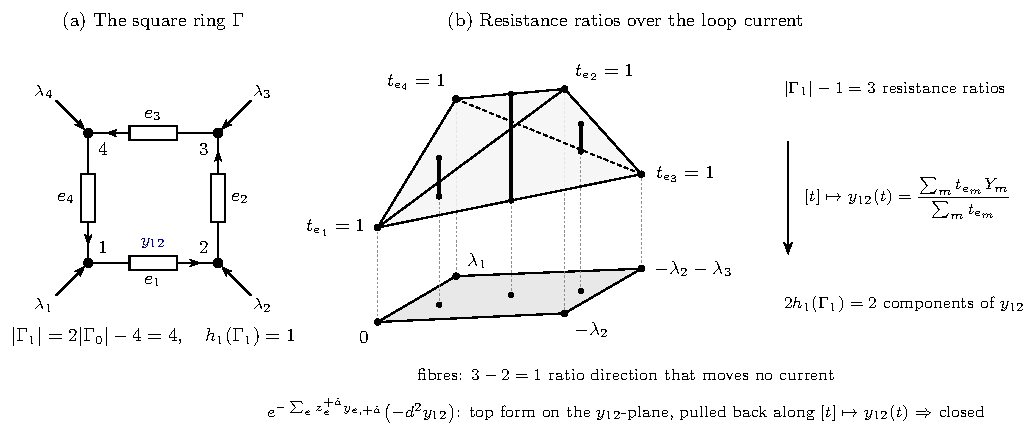
\includegraphics[width=0.98\linewidth]{figures/circuits/sc_almost.pdf}
\caption{An almost-Laman network: the square ring, $\Gamma_1=(e_1,e_2,e_3,e_4)$, $|\Gamma_1|=2|\Gamma_0|-4$. (a) The ring; $y_{12}$ is the current through $e_1$. (b) The $|\Gamma_1|-1=3$ resistance ratios form a tetrahedron, drawn so that $[t]\mapsto y_{12}(t)=\sum_mt_{e_m}Y_m/\sum_mt_{e_m}$ is the vertical projection onto the quadrilateral of the tree currents $Y_1=0$, $Y_2=-\lambda_2$, $Y_3=-\lambda_2-\lambda_3$, $Y_4=\lambda_1$; the vertex $t_{e_m}=1$ lies over $Y_m$. Each fibre (thick) is a segment along which the ratios change and no current moves; the longest joins the edges $t_{e_2}=t_{e_4}=0$ and $t_{e_1}=t_{e_3}=0$ over the crossing of the diagonals. The current form $e^{-\sum_ez_e^{+\dot a}y_{e,+\dot a}}(-d^2y_{12})$ is a top form on the $y_{12}$-plane pulled back to the ratios, hence closed (Lemma~\ref{lem:sc-closed}).}
\label{fig:sc-almost}
\end{figure}


\paragraph{Zooming into a short.}
For every $\emptyset\ne\gamma\subseteq\Gamma_1$ record the resistance ratios inside $\gamma$, $\bigl(t_e/\sum_{h\in\gamma}t_h\bigr)_{e\in\gamma}$, a point of a closed simplex. The closure of $\mathbb{RP}^{|\Gamma_1|-1}_{>0}$ in the product of these simplices is compact; it is the compactified Schwinger space modulo rescaling, $\widehat{(0,+\infty)^{|\Gamma_1|}}/\mathbb R_+$, of \cite[Definition 13, Remark 8, Proposition 7]{Wang}. A flag $\emptyset=\gamma_0\subsetneq\gamma_1\subsetneq\cdots\subsetneq\gamma_m\subsetneq\gamma_{m+1}=\Gamma_1$ gives the chart
\begin{equation}\label{eq:sc-chart}
t_e=s_is_{i+1}\cdots s_m\,r_e\quad(e\in\gamma_i\setminus\gamma_{i-1}),\qquad
\sum_{e\in\gamma_i\setminus\gamma_{i-1}}r_e=1,\qquad s\in[0,\infty)^m,
\end{equation}
with $r$ in the product of open simplices: at $s_i=0$ the resistors of $\gamma_i$ shrink infinitely faster than those of $\gamma_{i+1}\setminus\gamma_i$, a short inside a short. Every recorded ratio is a quotient of polynomials in $(s,r)$ with nonnegative coefficients, its denominator containing $\sum_{h\in\gamma\cap(\gamma_i\setminus\gamma_{i-1})}r_h$, with $\gamma_i\setminus\gamma_{i-1}$ the least shrunk layer meeting $\gamma$, hence positive; $r_e$ and $s_i$ are quotients of recorded ratios. These charts cover the closure (order the resistances by the rate at which they shrink) and make it a manifold with corners. Its faces of codimension one are the flags with $m=1$, one for each $\emptyset\ne\gamma\subsetneq\Gamma_1$:
\begin{equation}\label{eq:sc-face}
\{s=0\}=\mathbb{RP}^{|\gamma|-1}_{>0}\times\mathbb{RP}^{|\Gamma_1\setminus\gamma|-1}_{>0},
\qquad s=\frac{\sum_{e\in\gamma}t_e}{\sum_{e\notin\gamma}t_e},
\end{equation}
the ratios inside the short times the ratios of the remaining resistors (Figure~\ref{fig:short-zoom}).

For $\gamma\subseteq\Gamma_1$ the islands are the connected components of $(\Gamma_0,\gamma)$ that contain resistors, $c(\gamma)$ is the number of components of $(\Gamma_0,\gamma)$ and $h_1(\gamma)=|\gamma|-|\Gamma_0|+c(\gamma)$. The shorted network $\Gamma/\gamma$ has the components of $(\Gamma_0,\gamma)$ as nodes, each carrying the sum of its sources, and the resistors $\Gamma_1\setminus\gamma$; a resistor with both terminals in one island is a self-loop of $\Gamma/\gamma$.

\begin{figure}[H]
\centering
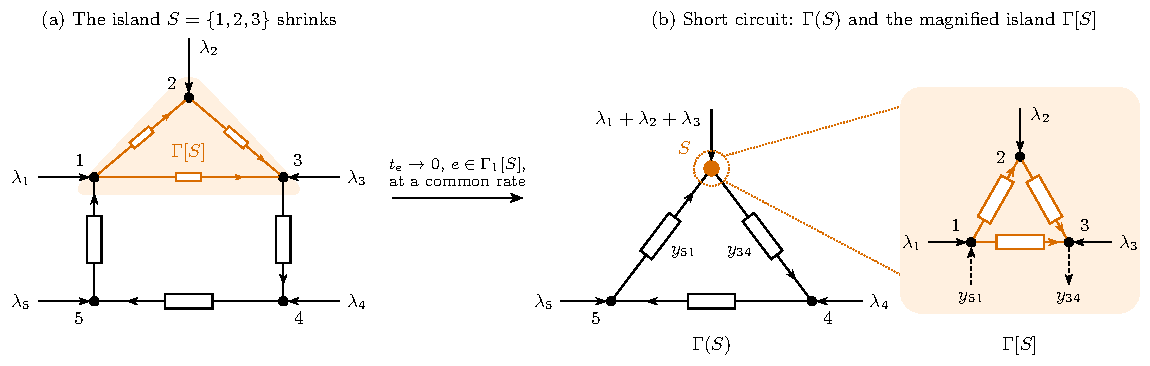
\includegraphics[width=0.98\linewidth]{figures/circuits/short_zoom.pdf}
\caption{The house, $\Gamma_1=(12,13,23,34,45,51)$, at the face where the roof $S=\{1,2,3\}$ shrinks. (a) The roof resistors shrink at a common rate. (b) On the face the roof is one node of the outer network $\Gamma(S)$, fed by $\lambda_1+\lambda_2+\lambda_3$; magnified, it is the network $\Gamma[S]$, fed by its own sources and by the currents $y_{51}$, $y_{34}$ that the outer resistors deliver to it and draw from it (dashed), as in \eqref{eq:sc-delivered}.}
\label{fig:short-zoom}
\end{figure}

\begin{lemma}[Tree sums at nested shorts]\label{lem:sc-trees}
In the chart \eqref{eq:sc-chart},
\begin{equation}\label{eq:sc-Ulead}
\sum_T\prod_{h\in\Gamma_1\setminus T}t_h
=\prod_{i=1}^{m}s_i^{\,h_1(\gamma_i)}
\Bigl[\prod_{i=1}^{m+1}\sum_{B_i}\prod_{h\in(\gamma_i\setminus\gamma_{i-1})\setminus B_i}r_h+O(s)\Bigr],
\end{equation}
$B_i$ running over the maximal spanning forests of $\gamma_i/\gamma_{i-1}$ (nodes: the components of $(\Gamma_0,\gamma_{i-1})$; resistors: $\gamma_i\setminus\gamma_{i-1}$). The bracket is a polynomial in $(s,r)$ with nonnegative coefficients, positive on the chart. Every numerator of \eqref{eq:1.24} is $\prod_is_i^{h_1(\gamma_i)}$ times a polynomial in $(s,r)$.
\end{lemma}
\begin{proof}
For a spanning tree $T$, $T\cap\gamma_i$ is a forest in $(\Gamma_0,\gamma_i)$, so
\[
\prod_{h\in\Gamma_1\setminus T}t_h=\prod_{i=1}^{m}s_i^{\,|\gamma_i\setminus T|}\prod_{h\in\Gamma_1\setminus T}r_h,
\qquad
|\gamma_i\setminus T|\ge|\gamma_i|-|\Gamma_0|+c(\gamma_i)=h_1(\gamma_i),
\]
with equality for every $i$ if and only if each $T\cap\gamma_i$ spans $(\Gamma_0,\gamma_i)$, that is, $T=B_1\sqcup\cdots\sqcup B_{m+1}$ with $B_i$ a maximal spanning forest of $\gamma_i/\gamma_{i-1}$.
\end{proof}

The dominant spanning trees omit as few shorted resistors as possible: each contains a spanning tree of every island and, outside the islands, a spanning tree of the shorted network (Figure~\ref{fig:sc-trees}). By Lemma~\ref{lem:sc-trees} the currents \eqref{eq:1.24} are quotients of polynomials in $(s,r)$ with denominators positive on every chart. They extend smoothly to $\widehat{(0,+\infty)^{|\Gamma_1|}}/\mathbb R_+$, and so does the integrand of \eqref{eq:sc-kernel}, closed by continuity.
\begin{figure}[H]
\centering
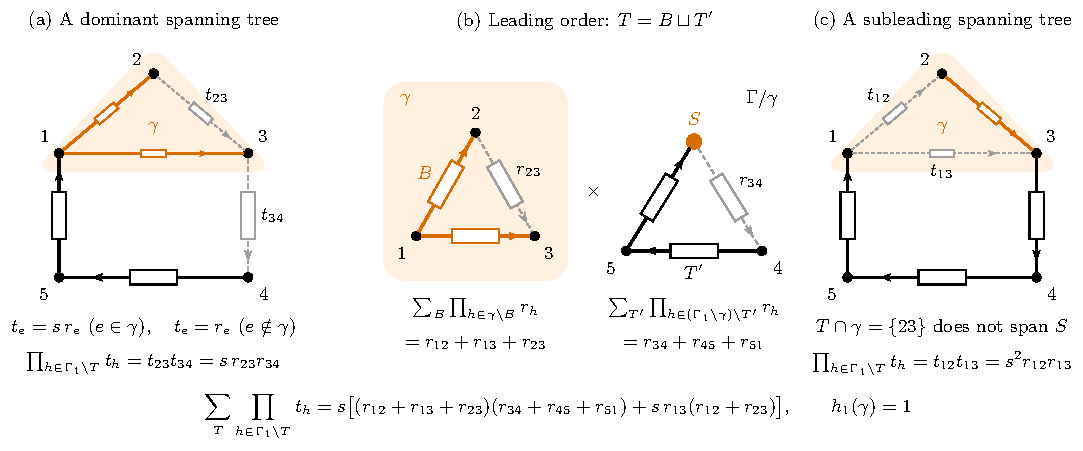
\includegraphics[width=0.98\linewidth]{figures/circuits/sc_trees.pdf}
\caption{Tree sums at the short of the roof of the house, $\gamma=\Gamma_1[S]$, $S=\{1,2,3\}$, in the chart $t_e=s\,r_e$ ($e\in\gamma$), $t_e=r_e$ ($e\notin\gamma$); thick: the spanning tree $T$, grey: the omitted resistors. (a) A dominant tree omits $h_1(\gamma)=1$ island resistor. (b) Its island part $B$ is a maximal spanning forest of $(\Gamma_0,\gamma)$ and its outer part $T'$ a spanning tree of $\Gamma/\gamma$; the dominant trees give the product of the two tree sums, as in \eqref{eq:sc-Ulead}. (c) A tree whose island part does not span $S$ omits two island resistors and is of order $s^2$.}
\label{fig:sc-trees}
\end{figure}


\begin{lemma}[Currents on a short]\label{lem:sc-currents}
On the face \eqref{eq:sc-face}:
\begin{enumerate}
\item[(i)] the resistors of $\Gamma_1\setminus\gamma$ carry the currents of the shorted network $\Gamma/\gamma$ with resistances $r_{\Gamma_1\setminus\gamma}$; a resistor joining two terminals of one island is bypassed by the short and carries no current;
\item[(ii)] the resistors of $\gamma$ carry the currents of the islands with resistances $r_\gamma$, fed at $v$ by
\begin{equation}\label{eq:sc-delivered}
\lambda^\gamma_{v,+\dot a}=\lambda_{v,+\dot a}
-\sum_{\substack{f\notin\gamma\\ f(0)=v}}y_{f,+\dot a}
+\sum_{\substack{f\notin\gamma\\ f(1)=v}}y_{f,+\dot a},
\end{equation}
its own source, minus the current the outer resistors carry away from $v$, plus the current they deliver to $v$ (Figure~\ref{fig:short-zoom}(b)). On each island these sources sum to zero.
\end{enumerate}
\end{lemma}
\begin{proof}
With $t_e=s\,r_e$ ($e\in\gamma$) and $t_e=r_e$ ($e\notin\gamma$), the voltage law \eqref{eq:C-oriented-cycle} around a cycle $C$ of $\Gamma$ reads
\[
\sum_{e\in C\setminus\gamma}\pm r_ey_{e,+\dot a}+s\sum_{e\in C\cap\gamma}\pm r_ey_{e,+\dot a}=0 .
\]
At $s=0$ the voltage drops across the islands disappear (Figure~\ref{fig:sc-currents}(a)). Every cycle of $\Gamma/\gamma$ lifts to a cycle of $\Gamma$ through paths in the islands, so the outer currents obey the voltage law of $\Gamma/\gamma$; a self-loop $f$ of $\Gamma/\gamma$, closed by a path in its island, gives $r_fy_f=0$ (Figure~\ref{fig:sc-currents}(b)). Summing \eqref{eq:1.9} over the nodes of one component of $(\Gamma_0,\gamma)$ cancels the island currents and gives the current law of $\Gamma/\gamma$ at that node, which also makes the $\lambda^\gamma_v$ sum to zero on each island. For a cycle $C\subseteq\gamma$ the relation is $s\sum_{e\in C}\pm r_ey_e=0$; dividing by $s>0$ and letting $s\to0$, the island currents obey the voltage law of the islands with resistances $r_\gamma$, and \eqref{eq:1.9} at $v$ is the current law of the islands with the sources $\lambda^\gamma_v$ (Figure~\ref{fig:sc-currents}(c)). The limits exist by Lemma~\ref{lem:sc-trees}; uniqueness of the network solutions gives (i) and (ii).
\end{proof}
\begin{figure}[H]
\centering
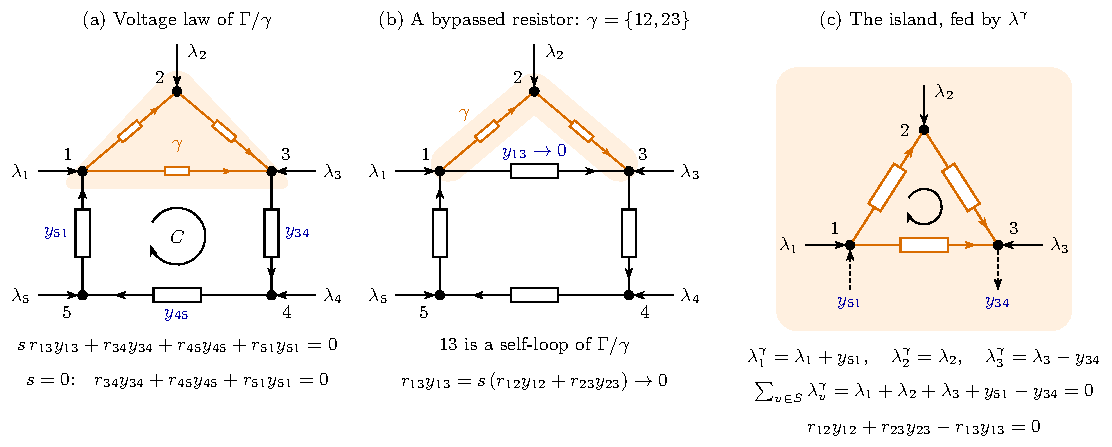
\includegraphics[width=0.98\linewidth]{figures/circuits/sc_currents.pdf}
\caption{Currents on a short of the house. (a) $\gamma=\Gamma_1[S]$: the cycle $C$ of $\Gamma$ through the island resistor $13$ lifts the triangle $34,45,51$ of $\Gamma/\gamma$; at $s=0$ the island carries no voltage drop and the outer currents obey the voltage law of $\Gamma/\gamma$. (b) $\gamma=\{12,23\}$: the resistor $13$ joins two terminals of the island, a self-loop of $\Gamma/\gamma$, and is bypassed. (c) The island of (a) with resistances $r_\gamma$, fed at $v$ by $\lambda^\gamma_v$ of \eqref{eq:sc-delivered}: its own source, plus $y_{51}$ delivered to $1$, minus $y_{34}$ carried away from $3$; the sources sum to zero by the current law of $\Gamma/\gamma$ at the merged node.}
\label{fig:sc-currents}
\end{figure}


\begin{lemma}[Island and outer network]\label{lem:sc-split}
Let $T=B\sqcup T'$, with $B$ a maximal spanning forest of $(\Gamma_0,\gamma)$ and $T'$ a spanning tree of $\Gamma/\gamma$. On the face \eqref{eq:sc-face},
\begin{equation}\label{eq:sc-split}
\begin{aligned}
e^{-\sum_ez_e^{+\dot a}y_{e,+\dot a}}\bigwedge_{e\notin T}\bigl(-d^2y_e\bigr)
={}&\Bigl[e^{-\sum_{e\in\gamma}z_e^{+\dot a}y_{e,+\dot a}}\bigwedge_{e\in\gamma\setminus B}\bigl(-d_\gamma^2y_e\bigr)\Bigr]\\
&\wedge\Bigl[e^{-\sum_{e\notin\gamma}z_e^{+\dot a}y_{e,+\dot a}}\bigwedge_{e\in(\Gamma_1\setminus\gamma)\setminus T'}\bigl(-d^2y_e\bigr)\Bigr],
\end{aligned}
\end{equation}
with $d_\gamma$ the differential along $\mathbb{RP}^{|\gamma|-1}_{>0}$ at fixed outer ratios. The first factor is the current form of the islands at the sources $\lambda^\gamma$, the second the current form of $\Gamma/\gamma$.
\end{lemma}
\begin{proof}
The chords of $T$ are $(\gamma\setminus B)\sqcup((\Gamma_1\setminus\gamma)\setminus T')$ (Figure~\ref{fig:sc-split}). By Lemma~\ref{lem:sc-currents} the outer currents depend only on the outer ratios, and for $e\in\gamma$
\[
dy_e=d_\gamma y_e+\sum_{v}\frac{\partial y_e}{\partial\lambda^\gamma_v}\,d\lambda^\gamma_v,
\qquad
d\lambda^\gamma_v\in\operatorname{span}\{dy_f:f\notin\gamma\}=\operatorname{span}\{dy_c:c\in(\Gamma_1\setminus\gamma)\setminus T'\},
\]
since the tree currents of $T'$ are affine in the chord currents of $\Gamma/\gamma$. The island learns about the outer network only through the currents delivered to it, and all $2h_1(\Gamma/\gamma)$ one-forms along which these move occur in the second factor, so the terms with $d\lambda^\gamma$ drop out.
\end{proof}
\begin{figure}[H]
\centering
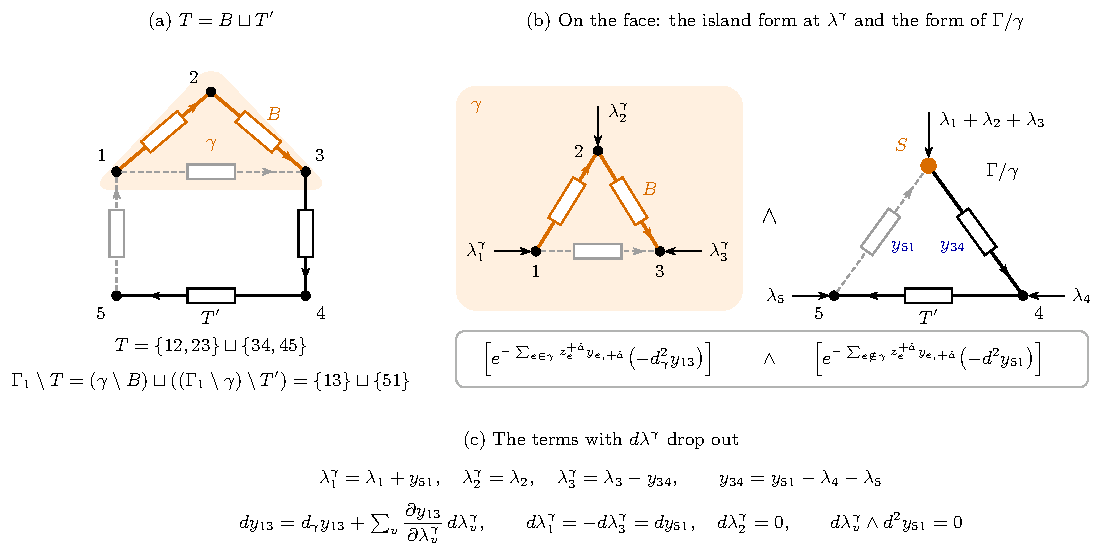
\includegraphics[width=0.98\linewidth]{figures/circuits/sc_split.pdf}
\caption{Island and outer network on the short of the roof. (a) $T=B\sqcup T'$ with $B=\{12,23\}$ a maximal spanning forest of $(\Gamma_0,\gamma)$ and $T'=\{34,45\}$ a spanning tree of $\Gamma/\gamma$; the chords (grey) are $13\in\gamma\setminus B$ and $51\in(\Gamma_1\setminus\gamma)\setminus T'$. (b) On the face \eqref{eq:sc-face} the current form splits as in \eqref{eq:sc-split}: the island form at the sources $\lambda^\gamma$ wedge the form of $\Gamma/\gamma$. (c) The island sources move only with the outer chord current $y_{51}$, whose two differentials already occur in $d^2y_{51}$.}
\label{fig:sc-split}
\end{figure}


\begin{proposition}[Contributing shorts]\label{prop:sc-faces}
Let $\Gamma$ be almost Laman. The integrand of \eqref{eq:sc-kernel} vanishes on the face of $\gamma$ unless $\gamma=\Gamma_1[S]$, the resistors of the induced subnetwork $\Gamma[S]$ on a set of nodes $S$, with
\begin{equation}\label{eq:sc-island}
\Gamma[S]\ \text{connected},\qquad |\Gamma_1[S]|=2|S|-3,\qquad 2\le|S|\le|\Gamma_0|-1 .
\end{equation}
Then $\Gamma/\gamma=\Gamma(S)$, the network with $\Gamma[S]$ shrunk to one node carrying $\sum_{v\in S}\lambda_v$ \cite[Section 3.5]{higher}, and $|\Gamma(S)_1|=2|\Gamma(S)_0|-3$.
\end{proposition}
\begin{proof}
(a) Degree. The two factors of \eqref{eq:sc-split} have degrees $2h_1(\gamma)$ and $2h_1(\Gamma/\gamma)$ along the two factors of \eqref{eq:sc-face}, and
\[
h_1(\gamma)+h_1(\Gamma/\gamma)=h_1(\Gamma_1),\qquad
2h_1(\Gamma_1)=|\Gamma_1|-2=\bigl(|\gamma|-1\bigr)+\bigl(|\Gamma_1\setminus\gamma|-1\bigr),
\]
so a nonzero top form requires
\[
2h_1(\gamma)=|\gamma|-1,\qquad 2h_1(\Gamma/\gamma)=|\Gamma_1\setminus\gamma|-1 .
\]
(b) Separate islands. If $\gamma$ has two or more islands $\gamma^{(1)},\gamma^{(2)},\ldots$, the island currents depend on $r_\gamma$ only through the ratios inside each island: the relative size of two islands shorted at a common rate moves no current (Figure~\ref{fig:short-vanishing}(b)). The first factor of \eqref{eq:sc-split} factors through a space of dimension $\sum_j(|\gamma^{(j)}|-1)\le|\gamma|-2$, below the degree $2h_1(\gamma)=|\gamma|-1$ required in (a), and vanishes.\\
(c) Bypassed resistor. A resistor $f\notin\gamma$ with both terminals in the island is a self-loop of $\Gamma/\gamma$, hence a chord of every $T'$, and $y_f=0$ on the face by Lemma~\ref{lem:sc-currents}(i) (Figure~\ref{fig:short-vanishing}(a)), so $d^2y_f=0$.\\
(d) Laman island. By (b) and (c), $\gamma=\Gamma_1[S]$ with $\Gamma[S]$ connected, $h_1(\gamma)=|\gamma|-|S|+1$, and
\[
2h_1(\gamma)=|\gamma|-1\iff|\Gamma_1[S]|=2|S|-3
\]
(Figure~\ref{fig:short-vanishing}(c)). $\gamma\ne\emptyset$ gives $|S|\ge2$; $\gamma\ne\Gamma_1$ gives $S\ne\Gamma_0$. Finally $|\Gamma(S)_1|=2|\Gamma_0|-4-(2|S|-3)=2(|\Gamma_0|-|S|+1)-3$.
\end{proof}

If two outer resistors join one node to two nodes of $S$, they are parallel in $\Gamma(S)$, and that face vanishes by \eqref{eq:1.13}.

\begin{figure}[H]
\centering
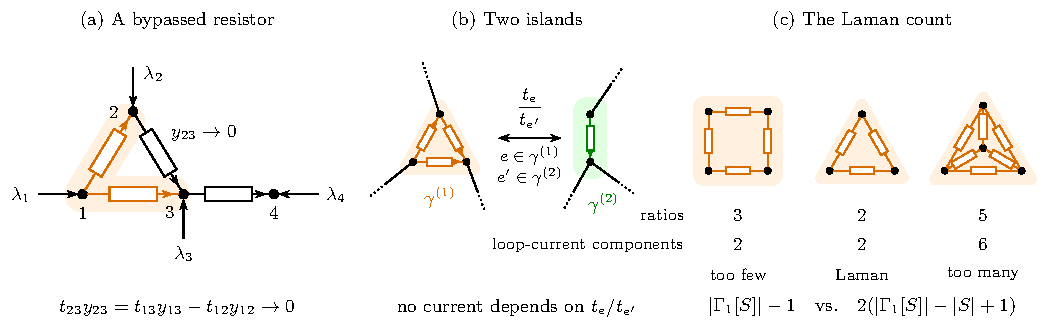
\includegraphics[width=0.98\linewidth]{figures/circuits/short_vanishing.pdf}
\caption{Faces without a contribution. (a) In the paw, $t_{12},t_{13}\to0$ at fixed $t_{23}$: the resistor $23$ joins two shorted nodes and carries no current. (b) Two islands shrinking at a common rate: no current depends on the ratio of their scales. (c) An island contributes only if its resistance ratios are as many as the real components of its loop currents: the square has too few resistors, the triangle is Laman, and $K_4$ has too many, which \eqref{eq:1.11} excludes.}
\label{fig:short-vanishing}
\end{figure}

\paragraph{The island is fed by the outer network.}
For $S$ as in \eqref{eq:sc-island} and $v\in S$, following \cite[Section 3.5]{higher},
\begin{equation}\label{eq:sc-lp}
(\lambda+\partial)_{v,+\dot a}
=\lambda_{v,+\dot a}
+\sum_{\substack{e(0)=v\\ e(1)\notin S}}\frac{\partial}{\partial z_e^{+\dot a}}
-\sum_{\substack{e(1)=v\\ e(0)\notin S}}\frac{\partial}{\partial z_e^{+\dot a}}
\end{equation}
(one symbol; $\partial_{v,+\dot a}$ alone keeps its meaning \eqref{eq:1.2}). Since $-\partial/\partial z_e^{+\dot a}$ inserts $y_{e,+\dot a}$ (Figure~\ref{fig:sc-fed}(a)),
\begin{equation}\label{eq:sc-insert}
(\lambda+\partial)_{v,+\dot a}\,e^{-\sum_{e\notin\Gamma_1[S]}z_e^{+\dot b}y_{e,+\dot b}}
=\Bigl(\lambda_{v,+\dot a}
-\sum_{\substack{f\notin\Gamma_1[S]\\ f(0)=v}}y_{f,+\dot a}
+\sum_{\substack{f\notin\Gamma_1[S]\\ f(1)=v}}y_{f,+\dot a}\Bigr)
e^{-\sum_{e\notin\Gamma_1[S]}z_e^{+\dot b}y_{e,+\dot b}} ,
\end{equation}
the island source $\lambda^\gamma_v$ of \eqref{eq:sc-delivered} for $\gamma=\Gamma_1[S]$: the signs of \eqref{eq:sc-lp} are those of Kirchhoff's current law. Summed over the island, with \eqref{eq:1.9} for $\Gamma(S)$ at the merged node (the shift identity of \cite[Section 3.5]{higher}),
\begin{equation}\label{eq:sc-sum}
\sum_{v\in S}(\lambda+\partial)_{v,+\dot a}\,\mathcal I^{\mathrm{raw\ cut}}_{\Gamma(S)}(\lambda;z)=0 .
\end{equation}

\begin{lemma}[Factorization of a short]\label{lem:sc-factor}
Let $\gamma=\Gamma_1[S]$. Each Taylor coefficient in $z$ of $\mathcal I^{\mathrm{raw\ cut}}_{\Gamma[S]}(\lambda^\gamma;z)$ is a polynomial in the island sources $\lambda^\gamma$, and the integral of \eqref{eq:sc-split} over $\mathbb{RP}^{|\Gamma_1[S]|-1}_{>0}\times\mathbb{RP}^{|\Gamma(S)_1|-1}_{>0}$ with the orientation $\eta_{\Gamma[S]}\wedge\eta_{\Gamma(S)}$ is
\begin{equation}\label{eq:sc-factor}
\mathcal I^{\mathrm{raw\ cut}}_{\Gamma[S]}(\lambda+\partial;z)\,\mathcal I^{\mathrm{raw\ cut}}_{\Gamma(S)}(\lambda;z),
\end{equation}
the resistors of $\Gamma[S]$ and $\Gamma(S)$ ordered as in $\Gamma$ and the operators $(\lambda+\partial)_v$ acting on $\mathcal I^{\mathrm{raw\ cut}}_{\Gamma(S)}$. By \eqref{eq:sc-sum}, \eqref{eq:sc-factor} does not depend on how the island polynomial is extended off $\sum_{v\in S}\lambda^\gamma_v=0$.
\end{lemma}
\begin{proof}
The island currents are linear in the island sources, so each Taylor coefficient of the first factor of \eqref{eq:sc-split} is a polynomial in $\lambda^\gamma$ times a form of top degree along $\mathbb{RP}^{|\Gamma_1[S]|-1}_{>0}$. Integrating over the island ratios first,
\[
\int\eqref{eq:sc-split}
=\int_{\mathbb{RP}^{|\Gamma(S)_1|-1}_{>0}}
\mathcal I^{\mathrm{raw\ cut}}_{\Gamma[S]}\bigl(\lambda^\gamma;z\bigr)\,
e^{-\sum_{e\notin\Gamma_1[S]}z_e^{+\dot a}y_{e,+\dot a}}\bigwedge_{c}\bigl(-d^2y_c\bigr),
\]
and by \eqref{eq:sc-insert} the sources $\lambda^\gamma$ are $(\lambda+\partial)$ acting on the exponential, outside the integral (Figure~\ref{fig:sc-fed}(b)).
\end{proof}
\begin{figure}[H]
\centering
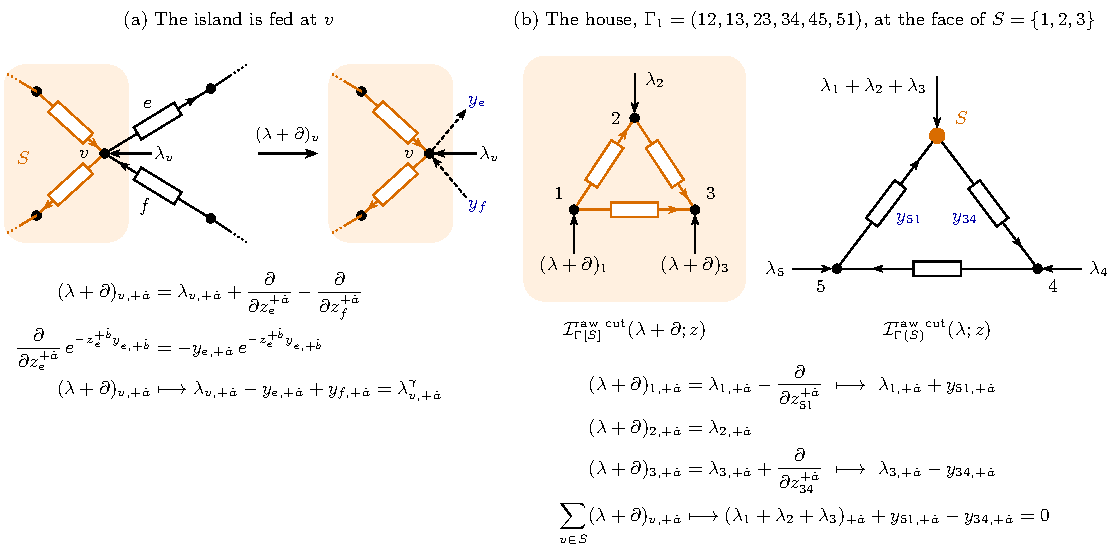
\includegraphics[width=0.98\linewidth]{figures/circuits/sc_fed.pdf}
\caption{The island fed by the outer network. (a) At $v\in S$ with an outer resistor $e$ leaving, $e(0)=v$, and $f$ entering, $f(1)=v$: $\partial/\partial z_e^{+\dot a}$ inserts $-y_{e,+\dot a}$ and $-\partial/\partial z_f^{+\dot a}$ inserts $y_{f,+\dot a}$, so $(\lambda+\partial)_v$ on the outer kernel feeds $v$ with $\lambda^\gamma_v$: its source, minus the current carried away, plus the current delivered (dashed). (b) The house at the face of $S=\{1,2,3\}$: the island kernel at the sources $(\lambda+\partial)_v$ times the outer kernel, \eqref{eq:sc-factor}; by the current law at the merged node the delivered sources sum to zero.}
\label{fig:sc-fed}
\end{figure}


\begin{lemma}[Orientation of a short]\label{lem:sc-orient}
For $\emptyset\ne\gamma\subsetneq\Gamma_1$ let $\pi_\gamma$ be the permutation of $\Gamma_1$ that moves the resistors of $\gamma$ to the front, keeping the relative order inside $\gamma$ and inside $\Gamma_1\setminus\gamma$. With the outward normal first, the face \eqref{eq:sc-face} is oriented as a boundary face of $\bigl(\widehat{(0,+\infty)^{|\Gamma_1|}}/\mathbb R_+,\eta_\Gamma\bigr)$ by
\begin{equation}\label{eq:sc-orient}
(-1)^{|\gamma|+1}\sgn(\pi_\gamma)\,\eta_\gamma\wedge\eta_{\Gamma_1\setminus\gamma}.
\end{equation}
For $\gamma=\Gamma_1[S]$ as in \eqref{eq:sc-island}, $|\gamma|=2|S|-3$ is odd and \eqref{eq:sc-orient} is $\sgn(\pi_S)\,\eta_{\Gamma[S]}\wedge\eta_{\Gamma(S)}$, $\pi_S=\pi_{\Gamma_1[S]}$.
\end{lemma}
\begin{proof}
In the collar coordinates $t_e=s\,r_e$ ($e\in\gamma$, $\sum_{e\in\gamma}r_e=1$) and $t_e=w_e$ ($e\notin\gamma$), $\bigwedge_{e\in\gamma}dr_e=0$, so
\[
\begin{gathered}
\bigwedge_{e\in\gamma}dt_e=s^{|\gamma|}\bigwedge_{e\in\gamma}dr_e+s^{|\gamma|-1}ds\wedge\eta_\gamma=s^{|\gamma|-1}ds\wedge\eta_\gamma,\\
dt_{e_1}\wedge\cdots\wedge dt_{e_{|\Gamma_1|}}=\sgn(\pi_\gamma)\,s^{|\gamma|-1}ds\wedge\eta_\gamma\wedge\bigwedge_{e\notin\gamma}dw_e .
\end{gathered}
\]
With $E=s\,\partial_s+\sum_{e\notin\gamma}w_e\partial/\partial w_e$ and $\iota_E\eta_\gamma=0$,
\[
\eta_\Gamma=\sgn(\pi_\gamma)\,s^{|\gamma|-1}\Bigl[s\,\eta_\gamma\wedge\bigwedge_{e\notin\gamma}dw_e-(-1)^{|\gamma|-1}ds\wedge\eta_\gamma\wedge\eta_{\Gamma_1\setminus\gamma}\Bigr].
\]
On the slice $\sum_{e\notin\gamma}w_e=1$ the first term vanishes:
\[
\eta_\Gamma=(-1)^{|\gamma|+1}\sgn(\pi_\gamma)\,s^{|\gamma|-1}\,(-ds)\wedge\eta_\gamma\wedge\eta_{\Gamma_1\setminus\gamma}.
\]
The interior is $s>0$ and the outward normal is $-\partial_s$.
\end{proof}

For two resistors $(a,b)$ in series (Figure~\ref{fig:sc-orient}(b)), $\eta_\Gamma=-ds$ on the slice $t_b=1$, with $s=t_a/t_b$: the short of $a$ ($s=0$) has orientation $+1$, the short of $b$ ($s=\infty$) has $-1=\sgn(\pi_{\{b\}})$.
\begin{figure}[H]
\centering
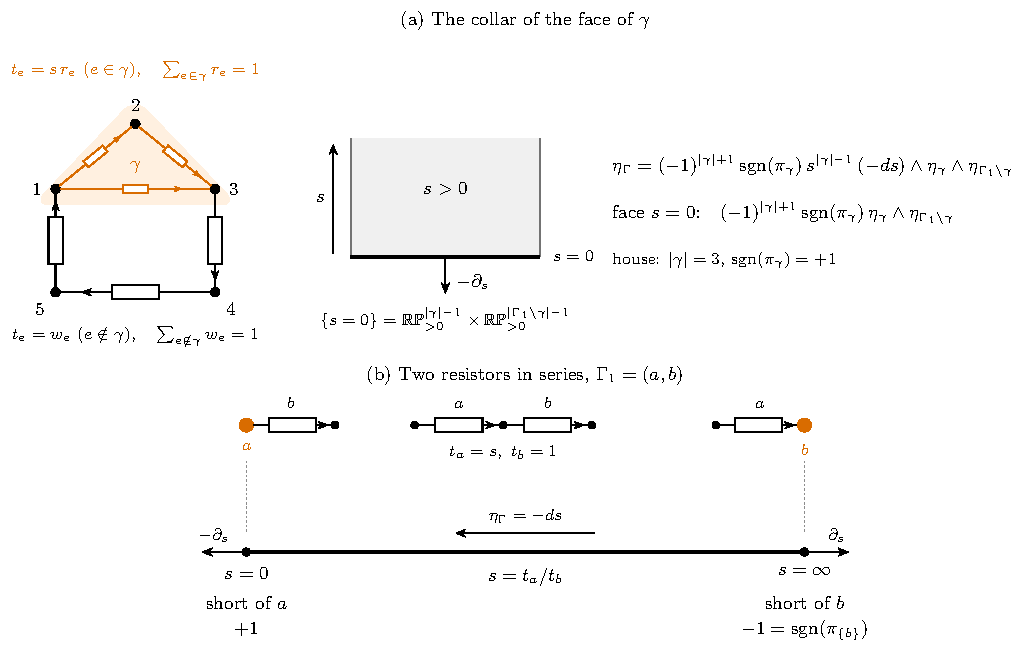
\includegraphics[width=0.92\linewidth]{figures/circuits/sc_orient.pdf}
\caption{(a) Collar of the face \eqref{eq:sc-face} of $\gamma$, on the house with the roof $\gamma=(12,13,23)$ shrinking: $t_e=s\,r_e$ on the island ($\sum_{e\in\gamma}r_e=1$), $t_e=w_e$ outside ($\sum_{e\notin\gamma}w_e=1$). The interior is $s>0$, the outward normal $-\partial_s$, and the face carries $(-1)^{|\gamma|+1}\sgn(\pi_\gamma)\,\eta_\gamma\wedge\eta_{\Gamma_1\setminus\gamma}$, here $+\eta_\gamma\wedge\eta_{\Gamma_1\setminus\gamma}$. (b) Two resistors $(a,b)$ in series: on the slice $t_b=1$, $\eta_\Gamma=-ds$ with $s=t_a/t_b$. The end $s=0$ shorts $a$ (orange node) and has orientation $+1$; the end $s=\infty$ shorts $b$ and has $-1=\sgn(\pi_{\{b\}})$.}
\label{fig:sc-orient}
\end{figure}


\begin{theorem}[Short-circuit identity]\label{thm:sc}
Let $\Gamma$ be a connected circuit without self-loops, with oriented resistors in a fixed order and $|\Gamma_1|=2|\Gamma_0|-4$. For sources with $\sum_{v\in\Gamma_0}\lambda_v=0$ and formal displacements $z$,
\begin{equation}\label{eq:sc-identity}
\sum_{S}\sgn(\pi_S)\,
\mathcal I^{\mathrm{raw\ cut}}_{\Gamma[S]}(\lambda+\partial;z)\,
\mathcal I^{\mathrm{raw\ cut}}_{\Gamma(S)}(\lambda;z)=0,
\end{equation}
summed over the $S\subseteq\Gamma_0$ of \eqref{eq:sc-island}. $\Gamma[S]$ and $\Gamma(S)$ keep the orientations and the relative order of their resistors in $\Gamma$, the merged node of $\Gamma(S)$ carries $\sum_{v\in S}\lambda_v$, $(\lambda+\partial)$ is \eqref{eq:sc-lp} and $\pi_S$ is the shuffle of Lemma~\ref{lem:sc-orient}. Terms in which $\Gamma(S)$ has parallel resistors vanish.
\end{theorem}
\begin{proof}
Let $\lambda$ be real. The integrand of \eqref{eq:sc-kernel} extends to $\widehat{(0,+\infty)^{|\Gamma_1|}}/\mathbb R_+$. By Lemma~\ref{lem:sc-closed}, Stokes' theorem on this compact manifold with corners (Figure~\ref{fig:sc-stokes}), Proposition~\ref{prop:sc-faces}, Lemma~\ref{lem:sc-orient} and Lemma~\ref{lem:sc-factor},
\[
\begin{aligned}
0&=\int_{\widehat{(0,+\infty)^{|\Gamma_1|}}/\mathbb R_+}d\Bigl(e^{-\sum_ez_e^{+\dot a}y_{e,+\dot a}}\bigwedge_{e\notin T}\bigl(-d^2y_e\bigr)\Bigr)
=\sum_{\emptyset\ne\gamma\subsetneq\Gamma_1}\int_{\{s=0\}}e^{-\sum_ez_e^{+\dot a}y_{e,+\dot a}}\bigwedge_{e\notin T}\bigl(-d^2y_e\bigr)\\
&=\sum_S\sgn(\pi_S)\int_{\mathbb{RP}^{|\Gamma_1[S]|-1}_{>0}\times\mathbb{RP}^{|\Gamma(S)_1|-1}_{>0}}\bigl(\text{right side of \eqref{eq:sc-split}}\bigr)\\
&=\sum_S\sgn(\pi_S)\,\mathcal I^{\mathrm{raw\ cut}}_{\Gamma[S]}(\lambda+\partial;z)\,\mathcal I^{\mathrm{raw\ cut}}_{\Gamma(S)}(\lambda;z).
\end{aligned}
\]
The face integrals carry the orientation $\eta_{\Gamma[S]}\wedge\eta_{\Gamma(S)}$; faces of codimension two and higher do not contribute. Each Taylor coefficient in $z$ is a polynomial in $\lambda$, so \eqref{eq:sc-identity} holds for all $\lambda$.
\end{proof}

With the shuffle sign $\sigma(\Gamma',\Gamma/\Gamma')$ of \cite[Section 4.1]{Wang}, which puts the outer resistors first, $(-1)^{\sigma(\Gamma[S],\Gamma/\Gamma[S])}=(-1)^{|\Gamma_1[S]|\,|\Gamma_1\setminus\Gamma_1[S]|}\sgn(\pi_S)=-\sgn(\pi_S)$ on every term of \eqref{eq:sc-identity}, both resistor counts being odd; \cite[Equation (4.8)]{Wang} at $d=2$ has the relative signs of \eqref{eq:sc-identity}.
\begin{figure}[H]
\centering
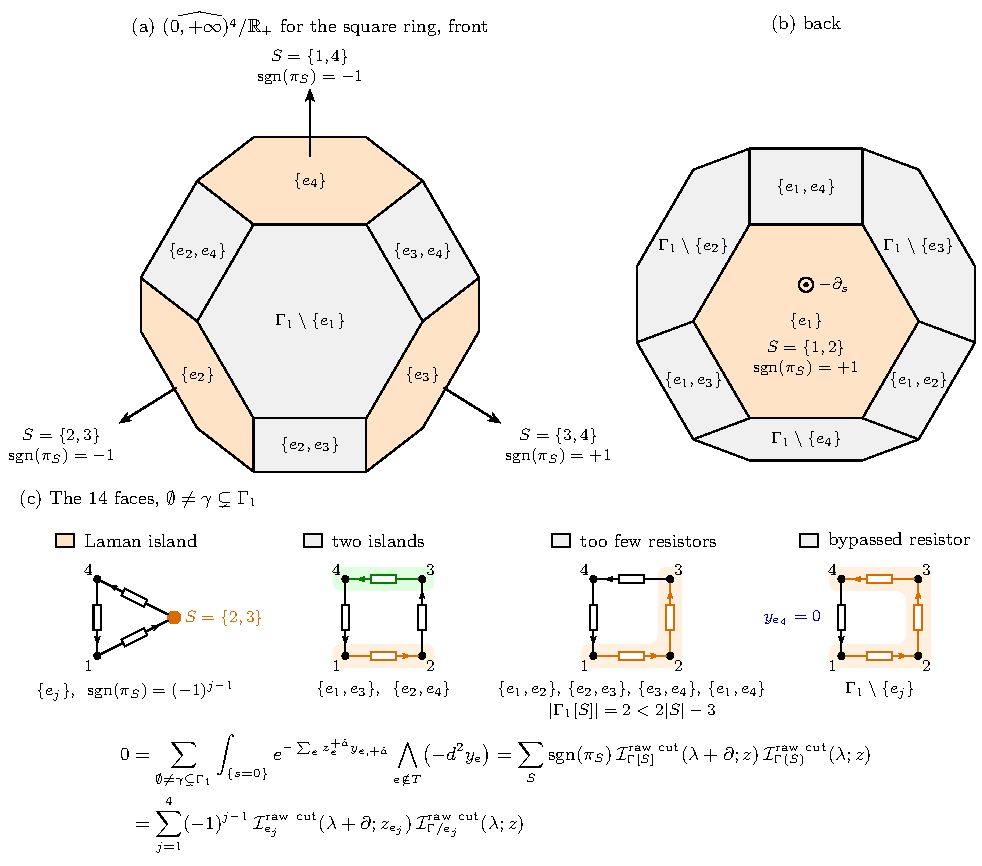
\includegraphics[width=0.9\linewidth]{figures/circuits/sc_stokes.pdf}
\caption{Stokes' theorem for the square ring, $\Gamma_1=(e_1,e_2,e_3,e_4)$. (a), (b) Front and back of $\widehat{(0,+\infty)^{4}}/\mathbb R_+$: one face $\{s=0\}$ for each $\emptyset\ne\gamma\subsetneq\Gamma_1$, two faces meeting along an edge when one $\gamma$ contains the other. The current form is closed, so its integrals over the fourteen faces, oriented with the outward normal $-\partial_s$ first, sum to zero. Only the Laman islands $\{e_j\}$ (orange) contribute, with $\operatorname{sgn}(\pi_S)=(-1)^{j-1}$. (c) The four kinds of faces: a Laman island, shrunk to a node of the triangle network $\Gamma(S)$; two islands; an island with too few resistors; a bypassed resistor. The last three carry no current form (Proposition~\ref{prop:sc-faces}).}
\label{fig:sc-stokes}
\end{figure}


\paragraph{Quadratic identities of the brackets.}
For $k$ entries, \eqref{eq:1.12} leaves circuits with $|\Gamma_1|=2k-3$ and $n=k-2$ loops. Inserting \eqref{eq:1.7} in \eqref{eq:A.28}, with the jet rule \eqref{eq:W-jet-edge} turning holomorphic derivatives of contracted letters into $z_e$-derivatives of the kernel and \eqref{eq:B.21} moving the letters left at node $v$ to the origin, with $\lambda_v=\partial/\partial x_v^+$ acting on them,
\begin{equation}\label{eq:sc-bracket-circuit}
\begin{aligned}
\{\mathcal O_1,\ldots,\mathcal O_k\}_0
={}&(-1)^{\sum_{i=1}^{k}(k-i)|\mathcal O_i|}(-8\pi^2)^{2-k}\\
&\times\sum_\Gamma\Bigl[\mathcal I^{\mathrm{raw\ cut}}_\Gamma(\lambda;z)\,W_\Gamma[\mathcal O_1,\ldots,\mathcal O_k]\Bigr]_{\lambda_v=\partial/\partial x_v^+,\ z=0},
\end{aligned}
\end{equation}
with $W_\Gamma[\mathcal O_1,\ldots,\mathcal O_k]=\Delta_{e_1}\Delta_{e_2}\cdots\Delta_{e_{|\Gamma_1|}}(\mathcal O_1\cdots\mathcal O_k)$ and $\Delta_e=\Delta_{e(0)e(1)}$ of \eqref{eq:A.20}, as in \eqref{eq:W-fibre-explicit}. Each $\Delta_e$ pairs an even with an odd letter:
\begin{equation}\label{eq:sc-odd}
\Delta_e\Delta_{e'}=-\Delta_{e'}\Delta_e,\qquad\Delta_e^2=0;
\end{equation}
$W_\Gamma$ and, through $\eta_\Gamma$, $\mathcal I^{\mathrm{raw\ cut}}_\Gamma$ both change sign under an odd reordering of the resistors, and their product does not. Relabelling ungrounded nodes permutes the circuits $\Gamma$, so $(-1)^{\sum_i(k-i)|\mathcal O_i|}\{\mathcal O_1,\ldots,\mathcal O_k\}_0$ depends on $\mathcal O_1,\ldots,\mathcal O_{k-1}$ only through the graded-commutative product $\mathcal O_1\cdots\mathcal O_k$:
\begin{equation}\label{eq:sc-exchange}
\{\ldots,\mathcal O_{i+1},\mathcal O_i,\ldots\}_0
=(-1)^{|\mathcal O_i||\mathcal O_{i+1}|+|\mathcal O_i|+|\mathcal O_{i+1}|}\{\ldots,\mathcal O_i,\mathcal O_{i+1},\ldots\}_0,
\qquad i+1<k .
\end{equation}
By \eqref{eq:1.2} and \eqref{eq:W-jet-edge}, on a letter of $\mathcal O_v$ that a resistor $e$ carries away,
\begin{equation}\label{eq:sc-jet}
\lambda_{v,+\dot a}=-\tfrac12\partial_{v,+\dot a}\ \longmapsto\
\begin{cases}
+\dfrac{\partial}{\partial z_e^{+\dot a}},&e(0)=v,\\[8pt]
-\dfrac{\partial}{\partial z_e^{+\dot a}},&e(1)=v.
\end{cases}
\end{equation}

Let $\Gamma$ be almost Laman on $k$ nodes, $S=\{i_1<\cdots<i_{|S|}\}$ as in \eqref{eq:sc-island}, $S^c=\{j_1<\cdots<j_{k-|S|}\}$, and place the island bracket $\{\mathcal O_{i_1},\ldots,\mathcal O_{i_{|S|}}\}_0$ at the merged node $\ast$ of an outer bracket (Figure~\ref{fig:sc-brackets}). An outer resistor at $\ast$ contracts a letter of the island bracket, that is, a letter of some $\mathcal O_v$, $v\in S$:
\begin{equation}\label{eq:sc-star}
\Delta_{\ast u}=\sum_{v\in S}\Delta_{vu}.
\end{equation}
By \eqref{eq:sc-jet} the island momentum $\lambda_v$ on the letters carried away by outer resistors becomes the $z$-derivatives of \eqref{eq:sc-lp}: the island is fed at $v$ by $(\lambda+\partial)_v$, its source plus the currents of the outer resistors at $v$ (Figure~\ref{fig:short-zoom}(b)). The outer source $\lambda_\ast=\sum_{v\in S}\lambda_v$ acts on the letters left in the output. The island bracket grounds the island at $i_{|S|}$: it replaces the island source $(\lambda+\partial)_{i_{|S|}}$ by $-\sum_{v\in S\setminus i_{|S|}}(\lambda+\partial)_v$, and the difference annihilates $\mathcal I^{\mathrm{raw\ cut}}_{\Gamma(S)}$ by \eqref{eq:sc-sum}, so the island may be grounded at any of its nodes. The node $k$ of $\Gamma$ stays grounded: for $k\in S$ the island bracket occupies the grounded slot. In both cases it is placed in the slot of its last entry,
\begin{equation}\label{eq:sc-slot}
P^{(S)}=\bigl(\mathcal O_{j_1},\ldots,\mathcal O_{j_p},\ \{\mathcal O_{i_1},\ldots,\mathcal O_{i_{|S|}}\}_0,\ \mathcal O_{j_{p+1}},\ldots,\mathcal O_{j_{k-|S|}}\bigr),\qquad j_p<i_{|S|}<j_{p+1}.
\end{equation}
By \eqref{eq:sc-star} the outer contractions act after the island contractions; with \eqref{eq:sc-odd},
\begin{equation}\label{eq:sc-W}
\begin{aligned}
\sgn(\pi_S)\,W_\Gamma
&=W_{\Gamma[S]}W_{\Gamma(S)}(\mathcal O_1\cdots\mathcal O_k)
=(-1)^{(2|S|-3)(2k-2|S|-1)}W_{\Gamma(S)}W_{\Gamma[S]}(\mathcal O_1\cdots\mathcal O_k)\\
&=-W_{\Gamma(S)}W_{\Gamma[S]}(\mathcal O_1\cdots\mathcal O_k),
\end{aligned}
\end{equation}
$W_{\Gamma[S]}$, $W_{\Gamma(S)}$ the ordered products of the $\Delta_e$ of $W_\Gamma$ over the island and over the outer resistors. The orientation sign of the short is the reordering sign of the contractions; the remaining $-1$ is common to all $S$. Multiplying \eqref{eq:sc-identity} by $W_\Gamma$,
\begin{equation}\label{eq:sc-identity-W}
\sum_S\mathcal I^{\mathrm{raw\ cut}}_{\Gamma[S]}(\lambda+\partial;z)\,\mathcal I^{\mathrm{raw\ cut}}_{\Gamma(S)}(\lambda;z)\,
W_{\Gamma(S)}W_{\Gamma[S]}(\mathcal O_1\cdots\mathcal O_k)=0 .
\end{equation}
The terms pair as
\[
\bigl(\Gamma',\ \Gamma'',\ \text{a node of }S\text{ for each outer resistor at }\ast\bigr)\ \longleftrightarrow\ (\Gamma,S),\qquad \Gamma[S]=\Gamma',\quad\Gamma(S)=\Gamma'' .
\]
A resistor of $\Gamma$ between two nodes of $S$ outside $\Gamma'$ would be a shorted resistor at $\ast$, so $\Gamma'$ is the induced subnetwork; two outer resistors from different nodes of $S$ to one node $u$ are parallel in $\Gamma''$, with kernel zero by \eqref{eq:1.13} and $\Delta_{\ast u}^2=0$. The normalizations combine to $(-8\pi^2)^{-(|S|-2)-(k-|S|-1)}=(-8\pi^2)^{3-k}$ for every $S$.
\begin{figure}[H]
\centering
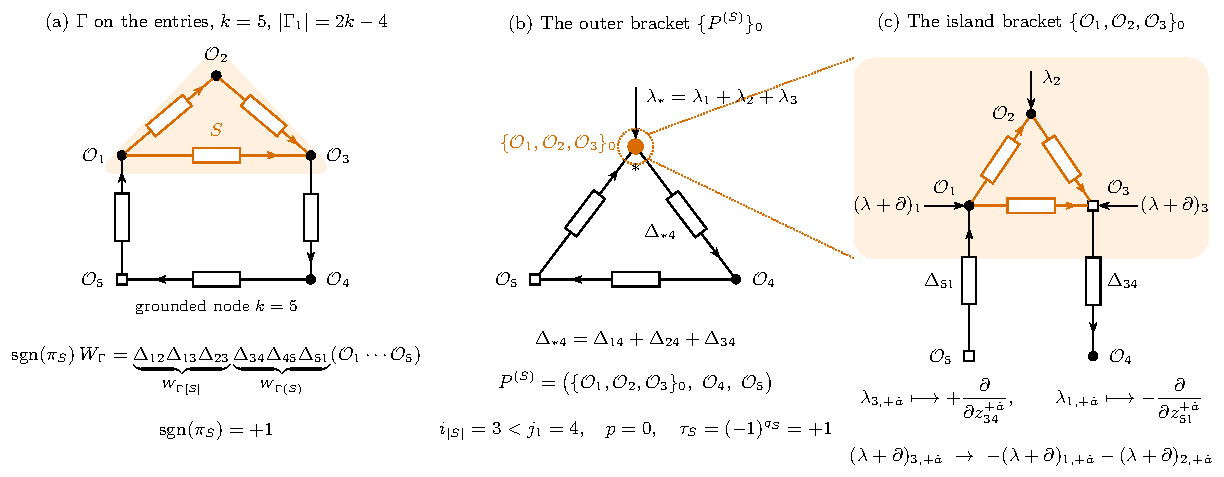
\includegraphics[width=0.98\linewidth]{figures/circuits/sc_brackets.pdf}
\caption{The term of $S=\{1,2,3\}$ for the house, $k=5$. (a) The entries $\mathcal O_1,\ldots,\mathcal O_5$ at the nodes, $\mathcal O_5$ grounded; $\operatorname{sgn}(\pi_S)W_\Gamma=W_{\Gamma[S]}W_{\Gamma(S)}(\mathcal O_1\cdots\mathcal O_5)$. (b) The outer bracket: the island bracket sits at the merged node $\ast$, in the slot of its last entry $i_{|S|}=3$; an outer resistor at $\ast$ contracts a letter of some $\mathcal O_v$, $v\in S$, and $\lambda_\ast$ acts on the letters left in the output. (c) The island bracket, grounded at $i_{|S|}=3$: the resistors $34$ and $51$ carry letters of $\mathcal O_3$ and $\mathcal O_1$ away, and the island is fed by the $(\lambda+\partial)_v$ of \eqref{eq:sc-lp}.}
\label{fig:sc-brackets}
\end{figure}


\begin{proposition}[Quadratic identities of the brackets]\label{prop:sc-brackets}
For $k\ge3$ homogeneous entries,
\begin{equation}\label{eq:sc-bracket-identity}
\sum_{S}\tau_S\,\{P^{(S)}\}_0=0,\qquad
\tau_S=(-1)^{\,q_S+|S|\,A_S^<+\sum_{(v,u)\in C_S}\left(|\mathcal O_u|+|\mathcal O_v|+|\mathcal O_u||\mathcal O_v|\right)},
\end{equation}
summed over $S\subseteq\{1,\ldots,k\}$ with $2\le|S|\le k-1$; $P^{(S)}$ is \eqref{eq:sc-slot}, $q_S=k-|S|-p$ is the number of entries after the island bracket, $A_S^<=\sum_{b\le p}|\mathcal O_{j_b}|$, and $C_S=\{(v,u)\in S\times S^c:\ v<u<i_{|S|}\}$.
\end{proposition}
\begin{proof}
Sum \eqref{eq:sc-identity-W} over $\Gamma$. By the pairing, the term of $S$ is the island bracket \eqref{eq:sc-bracket-circuit} of $(\mathcal O_{i_1},\ldots,\mathcal O_{i_{|S|}})$ inside the outer bracket \eqref{eq:sc-bracket-circuit} of $P^{(S)}$, up to signs from three sources: the prefactors of the two brackets, with $|\{\mathcal O_{i_1},\ldots,\mathcal O_{i_{|S|}}\}_0|\equiv\sum_{v\in S}|\mathcal O_v|+1$; the odd island operation $W_{\Gamma[S]}$ ($2|S|-3$ factors) moved past $\mathcal O_{j_1}\cdots\mathcal O_{j_p}$, giving $(-1)^{A_S^<}$; and the reordering $\mathcal O_{j_1}\cdots\mathcal O_{j_p}\mathcal O_{i_1}\cdots\mathcal O_{i_{|S|}}\mathcal O_{j_{p+1}}\cdots=(-1)^{\sum_{(v,u)\in C_S}|\mathcal O_u||\mathcal O_v|}\mathcal O_1\cdots\mathcal O_k$. The normalizations give the common factor $(-8\pi^2)^{3-k}$. After multiplication by the $S$-independent sign $(-1)^{\sum_i(k-i)|\mathcal O_i|}$, the sign of the term of $S$ is $(-1)$ to the power
\[
\begin{aligned}
&\sum_{i}(k-i)|\mathcal O_i|+\sum_{c=1}^{|S|}(|S|-c)|\mathcal O_{i_c}|
+q_S\Bigl(1+\sum_{v\in S}|\mathcal O_v|\Bigr)\\
&+\sum_{b\le p}(k-|S|+1-b)|\mathcal O_{j_b}|+\sum_{b>p}(k-|S|-b)|\mathcal O_{j_b}|
+A_S^<+\sum_{(v,u)\in C_S}|\mathcal O_u||\mathcal O_v| .
\end{aligned}
\]
Modulo 2, with $i_c-c=\#\{u\in S^c:u<i_c\}$, $j_b-b=\#\{v\in S:v<j_b\}$ and $p=\#\{u\in S^c:u<i_{|S|}\}$, the coefficient of $|\mathcal O_{i_c}|$ is $\#\{u\in S^c:\ i_c<u<i_{|S|}\}$, that of $|\mathcal O_{j_b}|$ is $|S|+\#\{v\in S:v<j_b\}$ for $b\le p$ and $0$ for $b>p$. This is $\tau_S$.
\end{proof}

Entries $(\mathcal I^{\otimes N},\mathcal O)$, $|\mathcal I|=0$, $k=N+1$: an island of $r$ interactions and $\mathcal O$ occupies the last slot, $\tau_S=+1$. For an island of $k'$ interactions with $i_{|S|}=N$, $q_S=1$ and $\tau_S=-1$; when $b$ interactions follow the island bracket, $\tau_S$ gains $(-1)^b$, and \eqref{eq:sc-exchange} moving the island bracket past them gives the same $(-1)^b$. The two types occur $\binom Nr$ and $\binom N{k'}$ times with equal terms, which is \eqref{eq:2.46}. Entries $(\mathcal I^{\otimes N},X,Y)$, $k=N+2$, with the islands of $k'$ interactions treated in the same way:
\[
\begin{array}{lccccc}
\text{island}&q_S&|S|&A_S^<&\sum_{C_S}&\tau_S\\[2pt]
r\ \mathcal I\text{'s},\ X,\ Y&0&r+2&0&0&+1\\
r\ \mathcal I\text{'s},\ X&1&r+1&0&0&-1\\
r\ \mathcal I\text{'s},\ Y&0&r+1&|X|&r|X|&(-1)^{|X|}\\
k'\ \mathcal I\text{'s},\ i_{|S|}=N&2&k'&0&0&+1
\end{array}
\]
The table gives \eqref{eq:quadratic-two}.

\paragraph{The paw.}
$\Gamma_1=((1,2),(1,3),(2,3),(3,4))$ (Figure~\ref{fig:short-paw}): three ratios, current form of degree $2$. The Laman islands are the four resistors and the triangle. Shorting a side of the triangle puts the other two sides in parallel (Figure~\ref{fig:short-paw}(e)); these faces vanish. Shorting the tail, $S=\{3,4\}$, $\sgn(\pi_S)=(-1)^3=-1$:
\[
\begin{aligned}
(\lambda+\partial)_{3,+\dot a}&=\lambda_{3,+\dot a}-\frac{\partial}{\partial z_{13}^{+\dot a}}-\frac{\partial}{\partial z_{23}^{+\dot a}},\\
\mathcal I^{\mathrm{raw\ cut}}_{\Gamma[S]}(\lambda+\partial;z)\,\mathcal I^{\mathrm{raw\ cut}}_{\Gamma(S)}(\lambda;z)
&=e^{-z_{34}^{+\dot a}(\lambda+\partial)_{3,+\dot a}}\,
\mathcal I^{\mathrm{raw\ cut}}_\triangle(\lambda_1,\lambda_2,\lambda_3+\lambda_4;z_{12},z_{13},z_{23})\\
&=e^{-\lambda_{3,+\dot a}z_{34}^{+\dot a}}\,
\mathcal I^{\mathrm{raw\ cut}}_\triangle(\lambda_1,\lambda_2,\lambda_3+\lambda_4;z_{12},z_{13}+z_{34},z_{23}+z_{34})\\
&=e^{\lambda_{4,+\dot a}z_{34}^{+\dot a}}\,
\mathcal I^{\mathrm{raw\ cut}}_\triangle(\lambda_1,\lambda_2,\lambda_3+\lambda_4;z_{12},z_{13},z_{23}),
\end{aligned}
\]
the last step since the resistors $13$ and $23$ deliver $y_{13}+y_{23}=\lambda_1+\lambda_2=-\lambda_3-\lambda_4$ into the node $\{3,4\}$. Shorting the triangle, $S=\{1,2,3\}$, $\sgn(\pi_S)=+1$; the outer network is the single lead $(\ast,4)$ carrying $\lambda_\ast=\lambda_1+\lambda_2+\lambda_3=-\lambda_4$, and the lead draws $y_{34}=-\lambda_4$ out of $3$:
\[
\begin{aligned}
(\lambda+\partial)_{3,+\dot a}&=\lambda_{3,+\dot a}+\frac{\partial}{\partial z_{34}^{+\dot a}},\qquad
\mathcal I^{\mathrm{raw\ cut}}_{\Gamma(S)}(\lambda;z)=e^{\lambda_{4,+\dot a}z_{34}^{+\dot a}},\\
\mathcal I^{\mathrm{raw\ cut}}_\triangle\bigl(\lambda_1,\lambda_2,(\lambda+\partial)_3;z_{12},z_{13},z_{23}\bigr)\,e^{\lambda_{4,+\dot a}z_{34}^{+\dot a}}
&=\mathcal I^{\mathrm{raw\ cut}}_\triangle(\lambda_1,\lambda_2,\lambda_3+\lambda_4;z_{12},z_{13},z_{23})\,e^{\lambda_{4,+\dot a}z_{34}^{+\dot a}} .
\end{aligned}
\]
The island of the second face and the outer network of the first are the same triangle network with the same resistor order, and the two terms cancel. The currents depend only on $t_{12}:t_{13}:t_{23}$; along $t_{34}/(t_{12}+t_{13}+t_{23})\in(0,\infty)$ nothing moves, and its two ends are the two contributing shorts (Figure~\ref{fig:short-paw}(b)).

\begin{figure}[H]
\centering
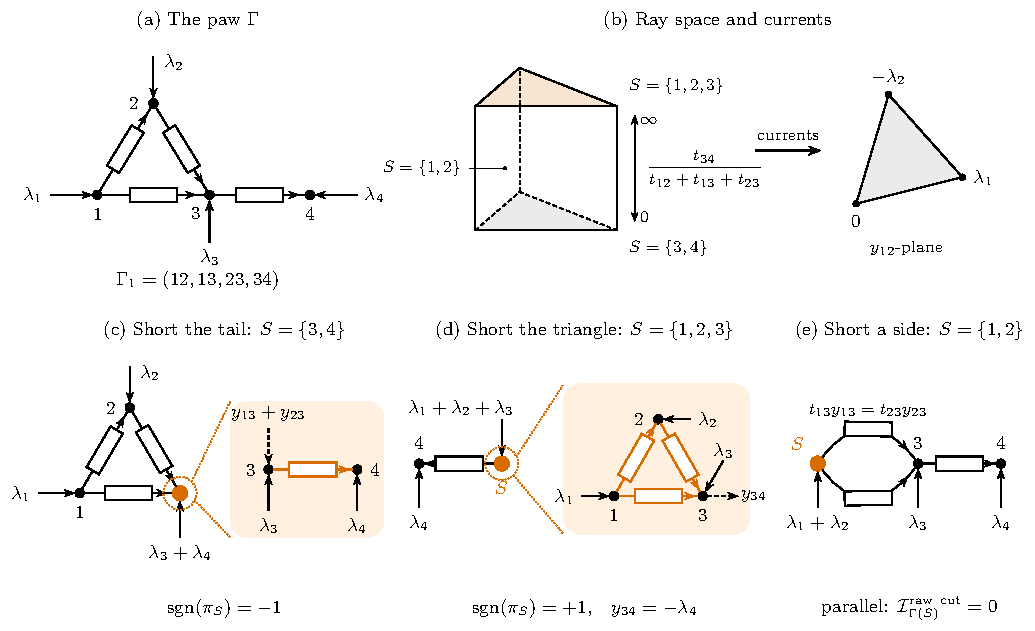
\includegraphics[width=0.98\linewidth]{figures/circuits/short_paw.pdf}
\caption{The paw, $\Gamma_1=(12,13,23,34)$. (b) The currents depend only on $t_{12}:t_{13}:t_{23}$; the ray space projects onto the triangle of the tree currents $y^T_{12}=0,\lambda_1,-\lambda_2$, and the ends $0$ and $\infty$ of the coordinate $t_{34}/(t_{12}+t_{13}+t_{23})$ are the faces (c) and (d). (c) Shorting the tail leaves the triangle network on $1$, $2$ and the node $\{3,4\}$, fed by $\lambda_3+\lambda_4$. (d) Shorting the triangle gives the same triangle network as the island; the lead draws $y_{34}=-\lambda_4$ out of $3$. (e) Shorting a side puts the other two sides in parallel.}
\label{fig:short-paw}
\end{figure}

\paragraph{The square ring.}
$\Gamma_1=(e_1,e_2,e_3,e_4)=((1,2),(2,3),(3,4),(4,1))$ (Figure~\ref{fig:short-square}). Three nodes of the ring span two resistors, so the Laman islands are the four resistors; shorting $e_j$ leaves a triangle network, and $\sgn(\pi_S)=(-1)^{j-1}$. A shorted single resistor $e=(v,w)$ carries the current fed into $v$, and its kernel shifts the displacements of the outer resistors at $v$:
\begin{equation}\label{eq:sc-single}
\begin{aligned}
&\mathcal I^{\mathrm{raw\ cut}}_{e}(\lambda+\partial;z_e)\,\mathcal I^{\mathrm{raw\ cut}}_{\Gamma/e}(\lambda;z)\\
&\qquad=e^{-\lambda_{v,+\dot a}z_e^{+\dot a}}\,
\mathcal I^{\mathrm{raw\ cut}}_{\Gamma/e}\bigl(\lambda;\ z_f-z_e\ (f(0)=v),\ z_f+z_e\ (f(1)=v)\bigr).
\end{aligned}
\end{equation}
\begin{figure}[H]
\centering
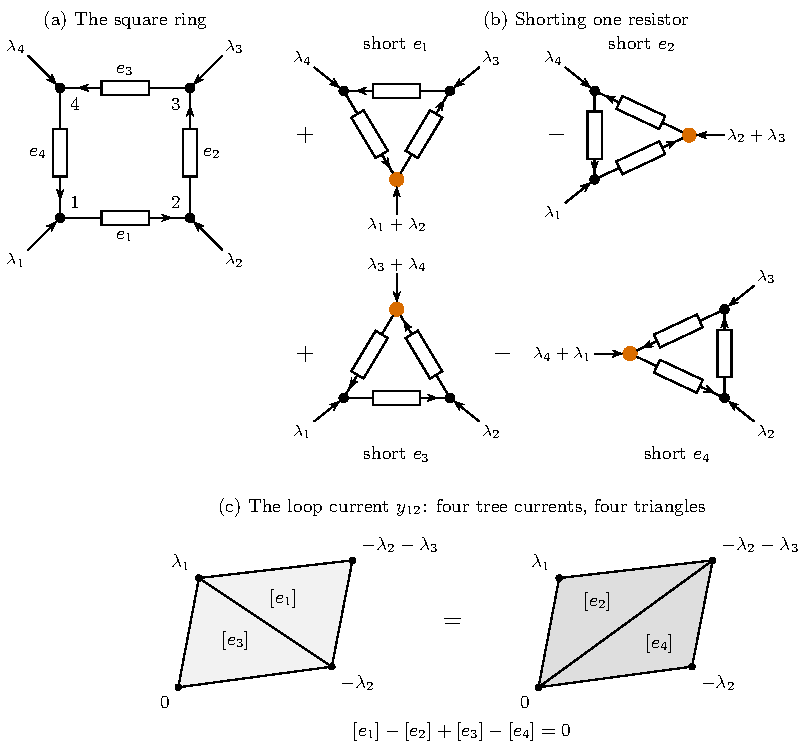
\includegraphics[width=0.85\linewidth]{figures/circuits/short_square.pdf}
\caption{The square ring. (b) Shorting $e_j$ merges its terminals and leaves a triangle network, with $\sgn(\pi_S)=(-1)^{j-1}$. (c) The loop current $y_{12}$ is the resistance-weighted average of the four tree currents $y^T_{12}$, $T=\Gamma_1\setminus\{e_m\}$; shorting $e_j$ leaves the triangle $[e_j]$ of the other three. The two diagonals give $[e_1]+[e_3]=[e_2]+[e_4]$.}
\label{fig:short-square}
\end{figure}
At $z=0$, where the resistor orientations drop out, the triangle kernel with resistor order $((a,b),(a,c),(b,c))$ is $\tfrac12\lambda_{a,+\dot a}\lambda_{b,+}{}^{\dot a}$ by \eqref{eq:1.25}:
\[
\begin{array}{lllll}
S&\sgn(\pi_S)&\Gamma(S)&(a,b,c)&\text{signed face at }z=0\\[2pt]
\{1,2\}&+1&(\ast3,34,4\ast)&(3,\ast,4)&+\tfrac12\lambda_{3,+\dot a}(\lambda_1+\lambda_2)_+{}^{\dot a}\\
\{2,3\}&-1&(1\ast,\ast4,41)&(\ast,1,4)&-\tfrac12(\lambda_2+\lambda_3)_{+\dot a}\lambda_{1,+}{}^{\dot a}\\
\{3,4\}&+1&(12,2\ast,\ast1)&(2,1,\ast)&+\tfrac12\lambda_{2,+\dot a}\lambda_{1,+}{}^{\dot a}\\
\{1,4\}&-1&(\ast2,23,3\ast)&(2,\ast,3)&-\tfrac12\lambda_{2,+\dot a}(\lambda_1+\lambda_4)_+{}^{\dot a}
\end{array}
\]
\[
\text{sum}=-\tfrac12\lambda_{2,+\dot a}(\lambda_1+\lambda_3+\lambda_4)_+{}^{\dot a}=\tfrac12\lambda_{2,+\dot a}\lambda_{2,+}{}^{\dot a}=0 .
\]
For general $z$: by \eqref{eq:1.24} the loop current is the resistance-weighted average of the four tree currents, $T_m=\Gamma_1\setminus\{e_m\}$ having weight $t_{e_m}$,
\[
y_{12}=\frac{\sum_mt_{e_m}Y_m}{\sum_mt_{e_m}},\qquad Y_1=0,\quad Y_2=-\lambda_2,\quad Y_3=-\lambda_2-\lambda_3,\quad Y_4=\lambda_1 ,
\]
so the tetrahedron of ratios maps affinely onto the quadrilateral of the $Y_m$, and shorting $e_j$ leaves the triangle of the other three (Figure~\ref{fig:short-square}(c)). With $X_m=-\sum_ez_e^{+\dot a}y^{T_m}_{e,+\dot a}$ and $\{a<b<c\}=\{1,2,3,4\}\setminus\{j\}$, the face of $e_j$ is
\[
\begin{aligned}
&\sgn(\pi_S)\,\mathcal I^{\mathrm{raw\ cut}}_{\Gamma[S]}(\lambda+\partial;z)\,\mathcal I^{\mathrm{raw\ cut}}_{\Gamma(S)}(\lambda;z)\\
&\qquad=(-1)^{j}\,(Y_b-Y_a)_{+\dot a}(Y_c-Y_a)_+{}^{\dot a}
\sum_{m\in\{a,b,c\}}\frac{e^{X_m}}{\prod_{l\in\{a,b,c\}\setminus\{m\}}(X_m-X_l)} ,
\end{aligned}
\]
the second divided difference of the exponential at the exponents $X_a,X_b,X_c$ of the remaining tree currents; the four faces cancel by Stokes' theorem on the tetrahedron. This is the four-term relation of \cite[Section 4.4]{operatope}.

\subsection{The Leibniz rule from short circuits}\label{sec:B-leibniz}

The Leibniz rule \eqref{eq:chain} is the part of the short-circuit identity \eqref{eq:sc-identity} that contracts the auxiliary pair of \eqref{eq:1.3}. For $N\ge1$, take the almost-Laman circuits \eqref{eq:sc-almost} on the interaction nodes $1,\ldots,N$ and the insertions $A=N+1$, $B=N+2$, which carry $Aa$ and $b_{\mathrm{aux}}B$; they have $2N$ resistors. The auxiliary letters contract only with each other, so a term survives $\mathrm{aux}=0$ only if the resistor $AB$ is present and contracts $a$ with $b_{\mathrm{aux}}$. This is the marked resistor, and the other $2N-1$ resistors contract fields of $\mathcal I$, $A$ and $B$ (Figure~\ref{fig:sc-leibniz}). A short that closes the marked resistor applies $\mathbf Q$ to the product; a short around one insertion applies $\mathbf Q$ to that factor, which the marked resistor then multiplies with the other; shorts of interactions alone assemble into the left side of \eqref{eq:2.40}; and the signed shorts of each circuit sum to zero.
\begin{figure}[t]
\centering
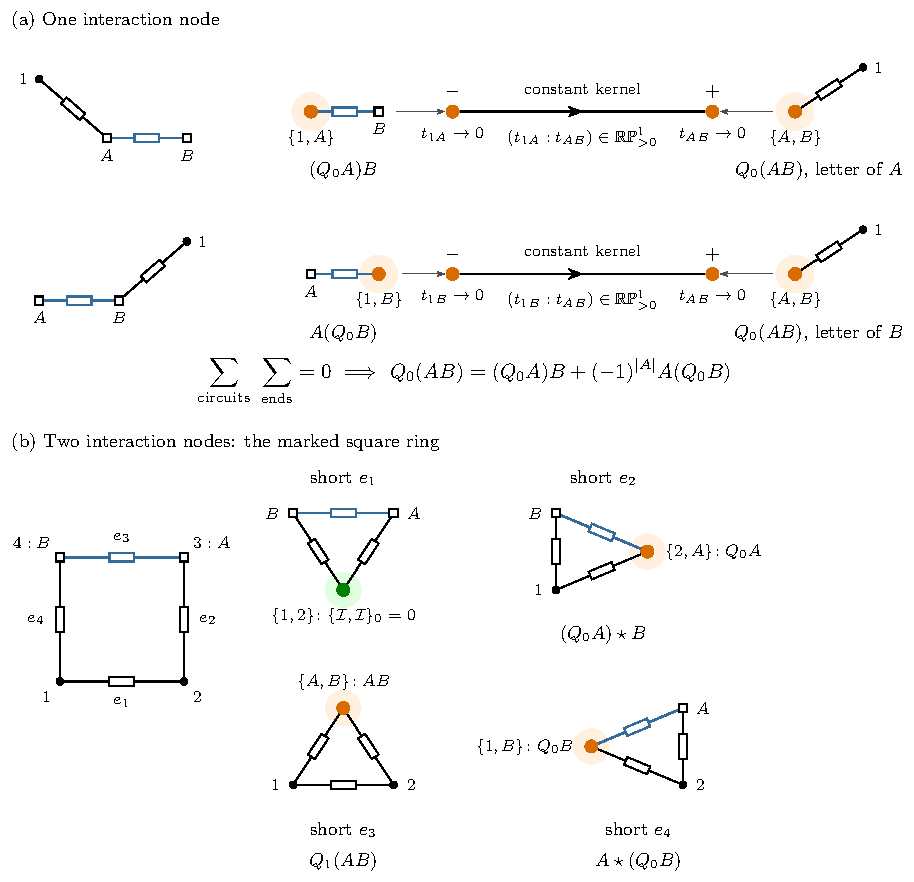
\includegraphics[width=0.96\linewidth,height=.8\textheight,keepaspectratio]{figures/circuits/sc_leibniz.pdf}
\caption{The Leibniz rule from shorts. Squares are the insertions, dots the interaction nodes, and the blue resistor is the marked resistor. An orange node is an island containing an insertion, a green node an island of interactions only, each labelled by the island and the composite it carries. (a) One interaction node: each ratio space is an interval with constant kernel, whose ends are the shorts of its two resistors; at the merged node $\{A,B\}$ the resistor contracts a letter of $A$ or of $B$. (b) Two interaction nodes: the square ring of Figure~\ref{fig:short-square} with $A=3$, $B=4$ and $e_3$ marked; its four shorts are the four kinds of Theorem~\ref{thm:sc-leibniz}, and those of $e_2$, $e_3$, $e_4$ give order-$\hbar$ terms of \eqref{eq:chain}.}
\label{fig:sc-leibniz}
\end{figure}

\begin{theorem}[Leibniz rule from short circuits]\label{thm:sc-leibniz}
Let the interaction satisfy \eqref{eq:2.40}. In the short-circuit identity of a marked almost-Laman circuit, every contributing island $S$, with $r$ interaction nodes, is of one of four kinds:
\begin{equation}\label{eq:sc-leibniz-kinds}
\begin{array}{l|l|l|l}
S\cap\{A,B\}&\text{merged node}&\text{outer network }\Gamma(S)&\text{sum over circuits}\\\hline
\{A,B\}&\{\mathcal I^{\otimes r},A,B\}^{\gamma,0}&\text{graph of }Q_{N-r-1}&\mathbf Q(A\star B)\\
\{A\}&\{\mathcal I^{\otimes r},A\}_0\,a&\text{marked graph}&(\mathbf QA)\star B\\
\{B\}&\{\mathcal I^{\otimes r},b_{\mathrm{aux}}B\}_0&\text{marked graph}&A\star(\mathbf QB)\\
\emptyset&\{\mathcal I^{\otimes r}\}_0&\text{marked graph}&0\text{ by \eqref{eq:2.40}}
\end{array}
\end{equation}
Weighted by $\hbar^{N-1}/N!$ and summed over all circuits and $N\ge1$, the shorts give the Leibniz rule \eqref{eq:chain}.
\end{theorem}
\begin{proof}
\emph{Stokes.} A marked almost-Laman circuit has one resistance ratio more than the real components of its loop currents, and its current form is closed (Lemma~\ref{lem:sc-closed}). Its integral over the boundary of the compactified ratio space vanishes. The boundary consists of shorts, and a short contributes only when its island $S$ is a Laman network, which the outer network $\Gamma(S)$ sees as a single node (Proposition~\ref{prop:sc-faces}, Theorem~\ref{thm:sc}).

\emph{Where the marked resistor goes.} A short closes every resistor between two nodes of its island. If $A,B\in S$, the marked resistor is shorted with the island, and the auxiliary pair is contracted inside it. If $A\in S$ and $B\notin S$, no resistor of the island reaches $B$: the letter $a$ rides to the merged node uncontracted, and the marked resistor joins the merged node to $B$ in the outer network. The same holds with $A$ and $B$ exchanged. If $A,B\notin S$, the marked resistor joins $A$ to $B$ outside the island.

\emph{What the merged node carries.} By Lemma~\ref{lem:sc-factor} and \eqref{eq:sc-slot}, the island fed by the outer network is the island bracket placed at the merged node.
\begin{enumerate}
\item[(i)] $A,B\in S$: the island is a marked graph of $\{\mathcal I^{\otimes r},A,B\}^{\gamma,0}$, $r!$ times the coefficient of $\hbar^r$ in $A\star B$. The outer network has $N-r$ interaction nodes, the merged node and $2(N-r+1)-3$ resistors: a graph of $Q_{N-r-1}$ acting on it.
\item[(ii)] $A\in S$, $B\notin S$: the island is a graph of $\{\mathcal I^{\otimes r},A\}_0=r!\,Q_{r-1}A$, with $a$ riding along, and the outer network, a marked graph with $N-r$ interaction nodes, multiplies it with $B$.
\item[(iii)] $B\in S$, $A\notin S$: as in (ii), with $A$ and $B$ exchanged.
\item[(iv)] $A,B\notin S$: the merged node carries $\{\mathcal I^{\otimes r}\}_0$, $r\ge2$, into a marked graph.
\end{enumerate}

\emph{Weights and signs.} Distributing the $N$ interaction nodes between the island and the outer network gives $\binom Nr$ equal terms, and $\binom Nr/N!=1/(r!\,(N-r)!)$ splits $\hbar^{N-1}/N!$ into the weights of $\mathbf Q$ in \eqref{eq:2.51} and of $\star$ in \eqref{eq:star}; in (iv), into the weight $\hbar^{r-2}/r!$ of \eqref{eq:2.40} and $\hbar^{N-r+1}/(N-r)!$ of the outer marked graph, as in \eqref{eq:quadratic-two-summed}. The orientation of each face, combined with the reordering of the contractions, gives the signs $\tau_S$ of Proposition~\ref{prop:sc-brackets}: by the table following it, $+1$, $-1$, $(-1)^{|Aa|}=(-1)^{|A|}$ and $+1$ for (i)--(iv). The four sums are the four terms of \eqref{eq:quadratic-two-summed} with $X=Aa$ and $Y=b_{\mathrm{aux}}B$ at $\mathrm{aux}=0$. The fourth vanishes by \eqref{eq:2.40}, and $\mathbf Q(b_{\mathrm{aux}}B)=-b_{\mathrm{aux}}\mathbf QB$ turns the third into $-(-1)^{|A|}A\star(\mathbf QB)$:
\[
0=\mathbf Q(A\star B)-(\mathbf QA)\star B-(-1)^{|A|}A\star(\mathbf QB).
\]
\end{proof}

\paragraph{One and two interaction nodes.}
For $N=1$ the marked almost-Laman circuits are the two paths $(1A,AB)$ and $(1B,AB)$ (Figure~\ref{fig:sc-leibniz}(a)). Their tree currents do not depend on the resistances, so the kernel is constant along the interval of ratios, and its two ends cancel. The short of $1A$ gives $(Q_0A)B$, the short of $1B$ gives $A(Q_0B)$, and the short of the marked resistor gives $Q_0(AB)$, the resistor at the merged node contracting a letter of $A$ or of $B$ by \eqref{eq:sc-star}:
\[
Q_0(AB)=(Q_0A)B+(-1)^{|A|}A(Q_0B).
\]
For $N=2$, the square ring of Figure~\ref{fig:short-square} with $A=3$, $B=4$ and the marked resistor $e_3$ has one short of each kind (Figure~\ref{fig:sc-leibniz}(b)). The short of $e_1$ closes the island $\{1,2\}$, whose $\{\mathcal I,\mathcal I\}_0$ vanishes by \eqref{eq:2.40}. The shorts of $e_2$ and $e_4$ close $\{2,A\}$ and $\{1,B\}$ and leave the one-loop marked triangles of $Q_0A$ with $B$ and of $A$ with $Q_0B$. The short of $e_3$ closes the marked resistor, and the triangle network on $1$, $2$ and the merged node is a graph of $Q_1$ acting on $AB$. The four faces are the four-term relation computed above.

\section{Heat-kernel transfer and the quantum differential}
\label{sec:quantum-transfer}

We review the BV construction of the holomorphically twisted theory
in Costello's formalism \cite{Costello}, using the ultraviolet finiteness of holomorphic graph integrals proved in \cite{Wang,WW}. Starting from the BV Ward
identity for an insertion, we rederive the loop corrections $Q_n$ of \cite{BK,higher} to
its local transformation and recover the graph formula
\eqref{eq:2.3} of Section~\ref{sec:supercharge}.

\subsection{Local inputs and their effective representatives}

The local data are the interaction density $\mathcal I$ and a
normal-ordered word $\mathcal O(0)$ in the zero-form fields
$\mathsf c,\mathsf b,\gamma,\beta$ and their holomorphic derivatives. Write
\begin{equation}\label{eq:C-local-inputs}
I=\int_{\mathbb C^2}\Omega\wedge[\mathcal I]_{(0,2)},
\qquad F=\mathcal O(0).
\end{equation}
The interaction density is the one in \eqref{eq:B.10}; its vertices
retain all Dolbeault components. Graph kernels are defined as distributions on smooth compactly
supported test densities. Translation invariance then permits fixing
the distinguished insertion at the origin.

The parameters $\varepsilon,L$ are the lower and upper limits of
Schwinger time in the propagator \eqref{eq:propagator}. With
$Q_{\mathrm{BV}}=\bar\partial$ and the gauge fixing of
Section~\ref{sec:setup},
\begin{equation}\label{eq:C-propagator-homotopy}
\begin{aligned}
h_{\varepsilon,L}&=\int_\varepsilon^L
 Q^{\mathrm{GF}}e^{-tH}\,dt,\\
\bar\partial h_{\varepsilon,L}+h_{\varepsilon,L}\bar\partial
&=e^{-\varepsilon H}-e^{-LH},\qquad
P_{\varepsilon,L}=(h_{\varepsilon,L}\otimes1)\omega_E^{-1}.
\end{aligned}
\end{equation}
Let $\partial_{P_{\varepsilon,L}}$ contract one unordered pair of
fields with $P_{\varepsilon,L}$, and let $\Delta_L$ contract a pair
with $K_L$, using the pairing \eqref{eq:A.20}. The prescribed
normal ordering omits self-contractions inside each local input.

In the holomorphic graph prescription used here, the effective
interaction and the representative of $\mathcal O$ are defined by
\begin{equation}\label{eq:C-local-to-effective}
\begin{aligned}
e^{I[L]/\hbar}
&=\lim_{\varepsilon\downarrow0}
 e^{\hbar\partial_{P_{\varepsilon,L}}}e^{I/\hbar},\\
F[L]e^{I[L]/\hbar}
&=\lim_{\varepsilon\downarrow0}
 e^{\hbar\partial_{P_{\varepsilon,L}}}
 \bigl(\mathcal O(0)e^{I/\hbar}\bigr).
\end{aligned}
\end{equation}
These limits are taken coefficientwise in perturbation theory as
graph distributions. Their ultraviolet finiteness for holomorphic
vertices is established in \cite[Corollary 4]{Wang}; the marked
insertion uses the same graph distributions with one distinguished
vertex. The logarithm in the first line selects connected interaction
graphs. Division by $e^{I[L]/\hbar}$ in the second selects the graphs
connected to the insertion. Their uncontracted fields can lie at
several positions, so $I[L]$ and $F[L]$ are effective functionals.
The original local word remains the label of $F[L]$.

The symbols $I[\varepsilon]$ and $F[\varepsilon]$ mean the same
effective families with upper scale $\varepsilon$. Splitting the
Schwinger interval gives the exact relations
\begin{equation}\label{eq:C-effective-insertion}
\begin{aligned}
e^{I[L]/\hbar}
&=e^{\hbar\partial_{P_{\varepsilon,L}}}e^{I[\varepsilon]/\hbar},\\
F[L]e^{I[L]/\hbar}
&=e^{\hbar\partial_{P_{\varepsilon,L}}}
 \bigl(F[\varepsilon]e^{I[\varepsilon]/\hbar}\bigr).
\end{aligned}
\end{equation}
At positive $\varepsilon$, these representatives already include
the graphs with smaller Schwinger times. Equation
\eqref{eq:C-local-to-effective} specifies their local input.

\subsection{The Ward identity defines the transformed insertion}

The propagator homotopy implies
\begin{equation}\label{eq:C-wick-intertwiner}
\begin{aligned}
[Q_{\mathrm{BV}},\partial_{P_{\varepsilon,L}}]
&=\Delta_\varepsilon-\Delta_L,\\
(Q_{\mathrm{BV}}+\hbar\Delta_L)e^{\hbar\partial_{P_{\varepsilon,L}}}
&=e^{\hbar\partial_{P_{\varepsilon,L}}}
 (Q_{\mathrm{BV}}+\hbar\Delta_\varepsilon).
\end{aligned}
\end{equation}
For the anomaly-free interaction considered in the main text,
the effective family satisfies the quantum master equation
\cite{Costello}:
\begin{equation}\label{eq:C-scale-QME}
Q_{\mathrm{BV}}I[L]+\frac12(I[L],I[L])_L
 +\hbar\Delta_LI[L]=0.
\end{equation}
Here $(\ ,\ )_L$ is the BV bracket defined by $K_L$, with the
product convention \eqref{eq:A-scale-bracket-sign}. Applying the
second-order operator to the insertion exponential gives
\begin{equation}\label{eq:C-full-quantum-BV}
\begin{aligned}
&e^{-I[L]/\hbar}(Q_{\mathrm{BV}}+\hbar\Delta_L)
 \bigl(e^{I[L]/\hbar}F[L]\bigr)\\
&\quad=Q_{\mathrm{BV}}F[L]+(I[L],F[L])_L+\hbar\Delta_LF[L]\\
&\qquad\quad+\frac1\hbar
 \left(Q_{\mathrm{BV}}I[L]+\frac12(I[L],I[L])_L
       +\hbar\Delta_LI[L]\right)F[L]\\
&\quad=Q_{\mathrm{BV}}F[L]+(I[L],F[L])_L+\hbar\Delta_LF[L].
\end{aligned}
\end{equation}
The last line is the BV transformation of the effective insertion.
It includes the variation of its surviving fields, contractions with
the effective interaction, and contractions within the insertion.

The projection $\pi$ of \eqref{eq:B.20} acts on each surviving
field by its holomorphic zero-form Taylor expansion at the insertion.
For any of the Dolbeault fields $X=\mathsf c,\mathsf b,\gamma,\beta$,
\begin{equation}\label{eq:C-field-projection}
X(x_v)\ \longmapsto\
\exp\!\left(x_v^{+\dot a}\frac{\partial}{\partial x^{+\dot a}}\right)
X^{(0)}(x)\big|_{x=0}.
\end{equation}
This substitution is applied after Wick contraction. The integration
coordinates and differential forms in the propagators remain in the
integral. The induced quantum differential is defined by
\begin{equation}\label{eq:C-insertion-definition}
\boxed{\displaystyle
\mathbf Q\mathcal O
=\pi\!\left[
 e^{-I[L]/\hbar}(Q_{\mathrm{BV}}+\hbar\Delta_L)
 \bigl(F[L]e^{I[L]/\hbar}\bigr)\right].}
\end{equation}
This is an insertion definition parallel to
\eqref{eq:C-local-to-effective}. The same fixed $L>0$ is used in
all its factors.

In this graph prescription $\pi F[L]=\mathcal O$. Indeed, a
nontrivial connected term has $m>0$ integrated interaction vertices.
After the field projection, the measure requires $2m$ propagators.
Each propagator is annihilated by contraction with the relative
antiholomorphic Euler vector:
\begin{equation}\label{eq:C-radial-propagator}
\iota_{\sum_{v=1}^{m}x_v^{-\dot a}\partial/\partial x_v^{-\dot a}}
 [P_{\varepsilon,L;e}]_\Omega=0.
\end{equation}
For an edge $(v,w)$, this is the identity
$\epsilon_{\dot a\dot b}(x_v-x_w)^{-\dot a}
(x_v-x_w)^{-\dot b}=0$. A top-degree form on the $2m$ relative
antiholomorphic coordinates with this property vanishes. Holomorphic
derivatives preserve the identity, and normal ordering removes
self-contractions at the root. Hence
\begin{equation}\label{eq:C-insertion-projection}
\pi F[L]=\mathcal O,\qquad
\pi Q_{\mathrm{BV}}=0,\qquad
\mathbf Q\mathcal O
=\pi\bigl((I[L],F[L])_L+\hbar\Delta_LF[L]\bigr).
\end{equation}
Thus the last expression acts on the same holomorphic words used
throughout the article.

\subsection{From the Ward identity to local heat-edge graphs}

Expand \eqref{eq:C-full-quantum-BV} using
\eqref{eq:C-local-to-effective}. Descent moves the free BV variation
of the surviving fields onto their incident propagators. With ordered
edges $e_1,\ldots,e_E$,
\begin{equation}\label{eq:C-heat-edge-cut}
\begin{aligned}
\bar\partial\bigwedge_{a=1}^{E}[P_{\varepsilon,L;e_a}]_\Omega
={}&\sum_{j=1}^{E}(-1)^{j-1}
\left(\bigwedge_{a<j}[P_{\varepsilon,L;e_a}]_\Omega\right)\\
&\wedge[K_{\varepsilon;e_j}-K_{L;e_j}]_\Omega
\wedge\left(\bigwedge_{a>j}[P_{\varepsilon,L;e_a}]_\Omega\right).
\end{aligned}
\end{equation}
The two upper-scale contractions in
\eqref{eq:C-insertion-projection} supply the $K_L$ terms with the
opposite sign; that these terms sum to the scale-$L$ bracket and Laplacian is the graph combinatorics of \cite[Lemma 2.7(2)]{WW}, cf.\ the boundary dictionary of \cite[Remark 12]{Wang}. The remaining $K_\varepsilon$ terms are the
ultraviolet boundaries of the insertion Ward identity. Boundary
components involving only interaction vertices cancel by
\eqref{eq:C-scale-QME}. A boundary containing the marked insertion
changes its local transformation law. This is the origin of the
loop corrections to $\mathbf Q$ \cite[Sections 2.2 and 4.1]{higher}.

Locality follows from the collision analysis of the graph
integrals \cite[Proposition 9 and Theorem 6]{Wang}. The total-collision
boundary is a differential operator supported on the full diagonal,
with derivatives only in holomorphic directions. For degree-zero
outputs on $k$ vertices, the contributing graphs have $2k-3$ edges.
Let $\Gamma^\prime$ be a proper Laman subgraph on $s$ vertices.
After it collapses, the quotient has
\begin{equation}\label{eq:C-quotient-count}
|\Gamma_0|-|\Gamma^\prime_0|+1=k-s+1,\qquad
|\Gamma_1|-|\Gamma^\prime_1|
=(2k-3)-(2s-3)=2(k-s).
\end{equation}
The remaining unmarked propagators form a top-degree wedge on its
$2(k-s)$ relative antiholomorphic coordinates. Equation
\eqref{eq:C-radial-propagator} makes this wedge zero. The
holomorphic derivatives supplied by the collapsing subgraph preserve
this vanishing. Consequently the projected coefficient comes entirely
from the total collision at the insertion.

Before projection, a collision containing the insertion leaves its
local transformed word attached to the remaining graphs. Summing these
graphs gives its effective representative
\cite[Proposition 11 and Corollary 6]{Wang}. The Ward identity therefore
also takes the form
\begin{equation}\label{eq:C-local-Ward-identity}
\begin{aligned}
&Q_{\mathrm{BV}}F[L]+(I[L],F[L])_L+\hbar\Delta_LF[L]\\
&\quad=(\mathbf Q\mathcal O)[L]\\
&\quad=e^{-I[L]/\hbar}\lim_{\varepsilon\downarrow0}
 e^{\hbar\partial_{P_{\varepsilon,L}}}
 \bigl((\mathbf Q\mathcal O)(0)e^{I/\hbar}\bigr).
\end{aligned}
\end{equation}
The notation $(\mathbf Q\mathcal O)[L]$ uses exactly the insertion
construction \eqref{eq:C-local-to-effective}, with local input
$\mathbf Q\mathcal O$. The total-collision boundary depends only on the ratios of the
Schwinger times and is independent of their upper endpoint $L$.
Since the projected proper-collision terms vanish, the local
coefficient in \eqref{eq:C-insertion-definition} is the same for
every $L>0$. Equation~\eqref{eq:C-local-Ward-identity} identifies
this coefficient with the quantum BV transformation of the insertion.

\subsection{The explicit local differential and the Schwinger scales}

For $m$ interaction vertices and one marked insertion, the projection
\eqref{eq:C-field-projection} retains only the zero-form output fields.
The heat edge supplies antiholomorphic degree two and each remaining
propagator degree one, saturating the $2m$ integration directions:

\begin{equation}\label{eq:C-loop-count}
|\Gamma_0|=m+1,\qquad
2+(|\Gamma_1|-1)=2m,\qquad
n=|\Gamma_1|-|\Gamma_0|+1=m-1.
\end{equation}
Each contraction contributes $\hbar$, and the expansion of
$e^{I/\hbar}$ contributes $1/(m!\hbar^m)$. Their product is
\begin{equation}\label{eq:C-loop-weight}
\frac{\hbar^{|\Gamma_1|-m}}{m!}
=\frac{\hbar^{m-1}}{m!}
=\frac{\hbar^n}{(n+1)!}.
\end{equation}
Using the ordered Wick operator of
\eqref{eq:W-fibre-explicit}--\eqref{eq:W-jet-edge}, the local
coefficient has the following explicit form:
\begin{equation}\label{eq:C-Qn-explicit}
\begin{aligned}
Q_n\mathcal O(0)
={}&\frac1{(n+1)!}
\sum_{\substack{\Gamma\ \mathrm{connected,\ labelled}\\
 |\Gamma_0|=n+2,\ |\Gamma_1|=2n+1}}
\lim_{\varepsilon\downarrow0}
\sum_{j=1}^{2n+1}(-1)^{j-1}
\pi\int_{(\mathbb C^2)^{n+1}}
 \left(\bigwedge_{v=1}^{n+1}\Omega_v\right)\\
&\times W_\Gamma\!\left[
 \left(\bigwedge_{a<j}[P_{\varepsilon,L;e_a}]_\Omega\right)
 \wedge[K_{\varepsilon;e_j}]_\Omega
 \wedge\left(\bigwedge_{a>j}[P_{\varepsilon,L;e_a}]_\Omega\right);\right.\\
&\hspace{7em}\left.
 \mathcal I(x_1),\ldots,\mathcal I(x_{n+1}),\mathcal O(0)
 \right].
\end{aligned}
\end{equation}
The upper Schwinger cutoff $L>0$ is fixed as $\varepsilon\downarrow0$. All edge orders, left derivatives and holomorphic displacement
variables are those of Appendix~\ref{sec:BV}. The interaction
density is even, so the global vertex sign in \eqref{eq:A.28}
is $+1$ for these ordered inputs. The Laman constraints eliminate
the other connected graphs. In the higher-bracket notation,
\begin{equation}\label{eq:C-transferred-Q}
\mathbf Q\mathcal O
=\sum_{n\ge0}\frac{\hbar^n}{(n+1)!}
 \{\mathcal I^{\otimes(n+1)},\mathcal O\}_0.
\end{equation}
At $n=0$ the single heat edge gives the classical bracket
$Q_0\mathcal O=\{\mathcal I,\mathcal O\}_0$; at $n=1$ the
three-edge triangle gives
$Q_1\mathcal O=\tfrac12\{\mathcal I,\mathcal I,\mathcal O\}_0$.

The scale parameters in \eqref{eq:C-Qn-explicit} are eliminated
when the local collision integral is evaluated. On a boundary with
$t_{e_j}=\varepsilon$, rescale all other edge Schwinger times and relative
positions by
\begin{equation}\label{eq:C-scale-removal}
t_e\longmapsto\varepsilon t_e,\qquad
x_v\longmapsto\sqrt\varepsilon\,x_v,\qquad
[\varepsilon,L]\longmapsto[1,L/\varepsilon],\qquad
L/\varepsilon\longrightarrow\infty.
\end{equation}
The total-collision coefficient retains the ratios of the edge Schwinger times.
Its common positive rescaling is removed by $\sum_e t_e=1$, giving
the projective Schwinger integral of Section~\ref{sec:setup}.
The unbounded interval arises for the rescaled Schwinger variables
because $L/\varepsilon\to\infty$ at fixed $L$
\cite[Sections 4.1--4.2]{Wang}. Displacement expansions are read
coefficientwise: the rescaling sends the output Taylor variables
to $\sqrt\varepsilon\,\lambda_v$ and each holomorphic displacement
to $z_e/\sqrt\varepsilon$. The surviving Taylor moment compensates
the powers of $\varepsilon$ from the input derivatives. The symbols $I[L]$ and $F[L]$ have completed
their role once this local coefficient is extracted; the main-text
calculations use only $\mathcal I$, $\mathcal O$, and its
kernel. The normalized finite-scale expression
\eqref{eq:C-insertion-definition} is evaluated at fixed $L$ before
passing to the projective kernel.

Finally, the QME makes the scale-$L$ BV differential square to zero.
Applying \eqref{eq:C-local-Ward-identity} twice and using
\eqref{eq:C-insertion-projection} gives
\begin{equation}\label{eq:C-square-zero}
\mathbf Q^2=0,\qquad
\sum_{r=0}^{n}Q_rQ_{n-r}=0\quad(n\ge0).
\end{equation}
These are also the quadratic identities of the local higher
operations \cite[Section 3]{operatope}, \cite[Equations (3.21) and (4.17)]{higher} (Stokes proof in \cite[Theorem 7]{Wang}), applied to the interacting brackets \cite[Equations (4.44)--(4.45)]{higher}.

\section{Feynman rules of the twisted theory}
\label{sec:feynman-rules}

This appendix collects, with their coefficients and signs, the rules from which every graph of the article is evaluated. The rules are those of the body, cited where they enter; the statements on coordinates, orientations and orderings make explicit the conventions these rules use. Appendix~\ref{sec:D-examples} evaluates examples with them.

\subsection{Coordinates, gradings and the Lie algebra}
\label{sec:D-conventions}

The coordinates and forms are those of \eqref{eq:Euclidean-coordinates}, \eqref{eq:coordinates} and the volume relation after \eqref{eq:B.7}:
\begin{equation}\label{eq:D-coordinates}
\begin{gathered}
x^{a\dot a}=x_E^\mu\sigma_\mu^{a\dot a},\qquad
\frac{\partial}{\partial x^{a\dot a}}=-\frac12\partial_{a\dot a},\qquad
\epsilon^{\dot+\dot-}=1=-\epsilon_{\dot+\dot-},\qquad
\epsilon^{+-}=1=-\epsilon_{+-},\\
dx^-_{\dot a}=\epsilon_{\dot a\dot b}dx^{-\dot b},\qquad
\bar\partial=dx^{-\dot a}\frac{\partial}{\partial x^{-\dot a}},\qquad
\Omega=2\,dx^{+\dot+}\wedge dx^{+\dot-},\qquad
\Omega\wedge dx^{-\dot+}\wedge dx^{-\dot-}=-8\,d^4x_E,\\
w_+{}^{\dot a}=\epsilon^{\dot a\dot b}w_{+\dot b},\qquad
u_{+\dot a}w_+{}^{\dot a}=u_{+\dot+}w_{+\dot-}-u_{+\dot-}w_{+\dot+},\qquad
|x|_E^2=x^{+\dot c}\epsilon_{\dot c\dot d}x^{-\dot d},
\end{gathered}
\end{equation}
with $d^4x_E=dx_E^0\wedge dx_E^1\wedge dx_E^2\wedge dx_E^3$. The last identity equates the exponents of \eqref{eq:C-heat-spatial} and \eqref{eq:C-explicit-propagator} at $z_e=0$; at real points $x^{-\dot a}$ is $\epsilon^{\dot a\dot b}$ times the complex conjugate of $x^{+\dot b}$, so that $|x|_E^2=\sum_{\dot a}|x^{+\dot a}|^2$. Integrals over $\mathbb C^2$ use the orientation of $d^4x_E$. The Lie algebra and matter representation satisfy
\begin{equation}\label{eq:D-lie}
[t_B,t_C]=iC^A{}_{BC}t_A,\qquad
C_{ABC}=\delta_{AD}C^D{}_{BC}=C_{[ABC]},\qquad
(t_A^{\mathrm{adj}})^B{}_C=iC^B{}_{AC},
\end{equation}
with Lie-algebra indices raised and lowered by $\delta$.

\begin{table}[H]
\centering\small
\caption{Fields of the twisted theory. Each is a Dolbeault form with components of antiholomorphic form degree $0,1,2$ \eqref{eq:field-form-dictionary}; a component is odd when its fermion number plus its form degree is odd.}
\label{tab:D-fields}
\begin{tabular}{lccccccc}
\toprule
field&$\mathsf c^A$&$\mathsf b_A$&$\gamma_i$&$\beta^i$&$\mathsf w_{\dot a}^A$&$a$&$b_{\mathrm{aux}}$\\
\midrule
fermion number&$1$&$0$&$0$&$1$&$1$&$0$&$1$\\
$\deg_\theta$ in $\mathcal N=4$ \eqref{eq:2.62}&$0$&$3$&$1$&$2$&&&\\
\bottomrule
\end{tabular}
\end{table}
\noindent The fermion number is the parity of a letter in the Koszul signs of (R4), unchanged by holomorphic derivatives. The output letters of every graph are the zero-form components and their holomorphic derivatives $\partial_{+\dot a}$.

\subsection{Action, interaction and pairing}
\label{sec:D-action}

The twisted action \eqref{eq:B.8}, its free part \eqref{eq:BV-free-action} and the interaction density \eqref{eq:B.10} are
\[
\begin{gathered}
S_{\mathrm{tw},E}=\int_{\mathbb C^2}\Omega\wedge\Big[
\mathsf b_A\Big(\bar\partial\mathsf c^A-\frac g2C^A{}_{BC}\mathsf c^B\mathsf c^C\Big)
+\big(\bar\partial\gamma_i-ig\mathsf c^A(t_A)^j{}_i\gamma_j\big)\beta^i
+\bar W(\gamma,\mathsf w)\Big]_{(0,2)},\\
S_{\mathrm{free}}=\int_{\mathbb C^2}\Omega\wedge
[\mathsf b_A\bar\partial\mathsf c^A+(\bar\partial\gamma_i)\beta^i]_{(0,2)},\qquad
Q_{\mathrm{BV}}=(S_{\mathrm{free}},\cdot)=\bar\partial,\\
\mathcal I=-\frac g2C^A{}_{BC}\mathsf b_A\mathsf c^B\mathsf c^C
-ig\mathsf c^A(t_A)^j{}_i\gamma_j\beta^i
+\bar W(\gamma,\mathsf w).
\end{gathered}
\]
After homotopy transfer $\mathsf w_{\dot a}^A\mapsto\frac12\partial_{+\dot a}\mathsf c^A=-\partial\mathsf c^A/\partial x^{+\dot a}$ \eqref{eq:retained-w}.

An edge between vertices $v,w$ contracts a $\mathsf c$ with a $\mathsf b$, or a $\gamma$ with a $\beta$. Its fibre operator is \eqref{eq:A.20},
\[
\Delta_{vw}=
\frac{\partial_L}{\partial\mathsf b_{A,v}}\frac{\partial_L}{\partial\mathsf c_w^A}
+\frac{\partial_L}{\partial\mathsf c_v^A}\frac{\partial_L}{\partial\mathsf b_{A,w}}
-\frac{\partial_L}{\partial\beta_v^i}\frac{\partial_L}{\partial\gamma_{i,w}}
-\frac{\partial_L}{\partial\gamma_{i,v}}\frac{\partial_L}{\partial\beta_w^i}.
\]
Each term contains one even and one odd left derivative, so $\Delta_{vw}=\Delta_{wv}$ and $\Delta_{vw}$ is odd. The first left fibre derivatives of the interaction are
\begin{equation}\label{eq:D-vertex}
\begin{aligned}
\frac{\partial_L\mathcal I}{\partial\mathsf b_A}&=-\frac g2C^A{}_{BC}\mathsf c^B\mathsf c^C,
&\frac{\partial_L\mathcal I}{\partial\mathsf c^D}&=-gC^A{}_{DC}\mathsf b_A\mathsf c^C-ig(t_D)^j{}_i\gamma_j\beta^i,\\
\frac{\partial_L\mathcal I}{\partial\gamma_k}&=-ig\mathsf c^A(t_A)^k{}_i\beta^i+\frac{\partial\bar W}{\partial\gamma_k},
&\frac{\partial_L\mathcal I}{\partial\beta^k}&=ig\mathsf c^A(t_A)^j{}_k\gamma_j;
\end{aligned}
\end{equation}
$\bar W$ depends on $\mathsf c$ only through $\mathsf w$, and the vertex factor $\partial_L\bar W/\partial\mathsf w^A_{\dot a}$ is contracted as $\frac12\partial_{+\dot a}\mathsf c^A$, carrying $-\partial/\partial z_e^{+\dot a}$ at a tail and $\partial/\partial z_e^{+\dot a}$ at a head of its edge \eqref{eq:W-jet-edge}.

In $\mathcal N=4$ Yang--Mills theory the fields form the superfield \eqref{eq:A.13} and the action is \eqref{eq:A.15},
\[
\begin{gathered}
C^A(\theta)=ig\,\mathsf c^A+\theta_I\delta^{AB}(\gamma^I)_B-\frac12\varepsilon^{IJK}\theta_I\theta_J(\beta_K)^A+\frac{\theta_1\theta_2\theta_3}{ig}\delta^{AB}\mathsf b_B,\\
S_{\mathrm{tw},E}=\int_{\mathbb C^2}\Omega\wedge
\Big[\int d^3\theta\Big(
\frac12\delta_{AB}C^A\bar\partial C^B
+\frac{i}{3!}C_{ABC}C^AC^BC^C\Big)\Big]_{(0,2)},
\end{gathered}
\]
with $\varepsilon^{123}=\varepsilon_{123}=1$, $\int d^3\theta\,\theta_1\theta_2\theta_3=1$, component order $\theta_IX$ and $Q_+^IC^A=\partial_LC^A/\partial\theta_I$. The odd operators $\bar\partial$ and $Q_0$ anticommute with $\theta_I$; with this rule the components of $Q_0C^A=\frac i2C^A{}_{BC}C^BC^C$ are \eqref{eq:B.15} for adjoint matter and the superpotential after \eqref{eq:A.15}. In components $\gamma_i\to(\gamma^I)_X$, $\beta^i\to(\beta_I)^X$ and $(t_A)^j{}_i\to(t^{\mathrm{adj}}_A)^Y{}_X\delta^I{}_J$, so that graphs can be evaluated with \eqref{eq:A.20}; the fibre derivative and pairing \eqref{eq:A.16}--\eqref{eq:A.17},
\[
\begin{gathered}
\frac{\delta}{\delta C^A(\theta)}
=\frac{\theta_1\theta_2\theta_3}{ig}\frac{\partial_L}{\partial\mathsf c^A}
-\frac12\varepsilon^{IJK}\theta_J\theta_K\frac{\partial}{\partial(\gamma^I)_A}
-\theta_I\frac{\partial_L}{\partial(\beta_I)^A}
-ig\frac{\partial}{\partial\mathsf b_A},\\
\frac{\delta C^B(\theta^{(2)})}{\delta C^A(\theta^{(1)})}=\delta_A{}^B\prod_{I=1}^3(\theta_I^{(1)}-\theta_I^{(2)}),\qquad
\Delta_{vw}=-\delta^{DE}\int d^3\theta\,\frac{\delta}{\delta C_v^D(\theta)}\frac{\delta}{\delta C_w^E(\theta)},
\end{gathered}
\]
collect the result into superfields, an oriented edge $(v,w)$ carrying the odd factor $\prod_{I=1}^3(\theta_I^{(v)}-\theta_I^{(w)})$. Each vertex carries $\frac i{3!}C_{ABC}C^AC^BC^C$ at its own odd coordinates $\theta^{(v)}$; the $3!$ assignments of its contracted and surviving letters to its three slots cancel the $1/3!$. At displaced points the functional derivative is normalized by \eqref{eq:2.10}.

\subsection{Edge kernels}
\label{sec:D-kernels}

Dolbeault gauge fixing uses $Q^{\mathrm{GF}}=\bar\partial^*$ and $H=\{\bar\partial,Q^{\mathrm{GF}}\}$. The heat kernel and propagator are \eqref{eq:propagator}, \eqref{eq:C-heat-spatial}, \eqref{eq:C-heat-homotopy} and \eqref{eq:C-explicit-propagator}:
\[
\begin{gathered}
[K_t(x_v,x_w)]_\Omega
=-\frac{e^{-|x_v-x_w|_E^2/(2t)}}{32\pi^2t^2}
 d(x_v-x_w)^{-\dot+}\wedge d(x_v-x_w)^{-\dot-},\\
[P_{\varepsilon,L;e}]_\Omega
=\frac{\epsilon_{\dot a\dot b}(x_v-x_w)^{-\dot a}d(x_v-x_w)^{-\dot b}}{32\pi^2}
 \int_\varepsilon^L\frac{dt_e}{t_e^3}
\exp\Big[-\frac{(x_v-x_w+z_e)^{+\dot c}\epsilon_{\dot c\dot d}(x_v-x_w)^{-\dot d}}{2t_e}\Big],
\end{gathered}
\]
for an oriented edge $e=(v,w)$. They are normalized by
\begin{equation}\label{eq:D-normalization}
\int_{\mathbb C^2}\Omega\wedge[K_t(x,0)]_\Omega=1,\qquad
(\bar\partial\otimes1+1\otimes\bar\partial)P_{\varepsilon,L}=K_\varepsilon-K_L,\qquad
\int_{S^3}\Omega\wedge[P_{0,\infty}]_\Omega=1,
\end{equation}
the first by $\Omega\wedge dx^{-\dot+}\wedge dx^{-\dot-}=-8\,d^4x_E$ and $\int d^4x_E\,e^{-|x|_E^2/(2t)}=4\pi^2t^2$, the last for $S^3$ positively oriented around the origin by \eqref{eq:ring-propagator-residue}.

The edge argument is $x_{e(0)}-x_{e(1)}+z_e$, with $z_e=z_{v,i}-z_{w,j}$ for the $i$th field at $v$ and the $j$th at $w$ \eqref{eq:input-displacement}. Since
\[
\partial_{v,+\dot a}[P_e]_\Omega=-2\frac{\partial}{\partial z_e^{+\dot a}}[P_e]_\Omega,\qquad
\partial_{w,+\dot a}[P_e]_\Omega=2\frac{\partial}{\partial z_e^{+\dot a}}[P_e]_\Omega,
\]
and likewise for the heat kernel, a holomorphic derivative on a contracted letter becomes a derivative of the edge kernel in its displacement, with $-2$ for the tail $v$ and $2$ for the head $w$ \eqref{eq:W-jet-edge}. Reversing the orientation of $e$ together with $z_e\mapsto-z_e$ leaves $[P_e]_\Omega$ and $[K_e]_\Omega$ unchanged; together with $\Delta_{vw}=\Delta_{wv}$, the value of a graph does not depend on the orientations of its edges. In Schwinger time the heat kernel and the propagator integrand combine into one form of the edge current \eqref{eq:1.8}, \eqref{eq:C-current-Jacobian}:
\[
\begin{gathered}
y_{e,+\dot a}=\frac{\epsilon_{\dot a\dot b}(x_{e(0)}-x_{e(1)})^{-\dot b}}{2t_e},\\
[K_{t_e;e}]_\Omega-dt_e\wedge[(Q^{\mathrm{GF}}\otimes1)K_{t_e;e}]_\Omega
=-\frac{1}{8\pi^2}\,e^{-(x_{e(0)}-x_{e(1)}+z_e)^{+\dot a}y_{e,+\dot a}}\,dy_{e,+\dot+}\wedge dy_{e,+\dot-}.
\end{gathered}
\]

\subsection{Graphs, signs and normalization}
\label{sec:D-graphs}

For homogeneous operators $\mathcal O_1,\ldots,\mathcal O_k$ with $\mathcal O_k$ at the origin, the bracket $\{\mathcal O_1,\ldots,\mathcal O_k\}_0$ of \eqref{eq:A.28} is evaluated by the following rules.
\begin{enumerate}
\item[(R1)] \emph{Graphs.} Sum over connected labelled graphs $\Gamma$ on the vertices $1,\ldots,k$, the vertex $v$ carrying $\mathcal O_v(x_v)$. The vertices are distinguishable: graphs that differ by a relabelling of interaction vertices are distinct terms, and no factor $1/|\mathrm{Aut}\,\Gamma|$ occurs. Each edge contracts a $\mathsf c$ with a $\mathsf b$ or a $\gamma$ with a $\beta$ at two different vertices, $\Delta_{vw}$ summing over the pairs of letters it can contract; contractions inside one input are excluded.
\item[(R2)] \emph{Order and orientation.} Order the edges $e_1,\ldots,e_{|\Gamma_1|}$ and orient them, $e_a=(v_a,w_a)$.
\item[(R3)] \emph{Spacetime factor.} For $j=1,\ldots,|\Gamma_1|$, the edge $e_j$ carries $[K_{\varepsilon;e_j}]_\Omega$ and every other edge $[P_{\varepsilon,L;e_a}]_\Omega$, wedged in edge order, with the sign $(-1)^{j-1}$; the $j$-sum is the action of $\bar\partial$ on the ordered propagators \eqref{eq:C-heat-edge-cut}, restricted to its lower boundaries.
\item[(R4)] \emph{Fibre factor.} The ordered contraction \eqref{eq:W-fibre-explicit} applies $\Delta_{v_1w_1}\Delta_{v_2w_2}\cdots\Delta_{v_{|\Gamma_1|}w_{|\Gamma_1|}}$ to the ordered product $\mathcal O_1\cdots\mathcal O_k$, the operators acting from right to left: $\Delta_{v_{|\Gamma_1|}w_{|\Gamma_1|}}$ first, and in each term of $\Delta_{vw}$ the right-hand derivative first. A left derivative $\partial_L/\partial X$ acquires $(-1)^{|X||Y|}$ for every letter $Y$ it passes, $|X|,|Y|$ the fermion numbers of Table~\ref{tab:D-fields}: $\partial_L/\partial\mathsf c$ and $\partial_L/\partial\beta$ acquire $-1$ for every odd letter, $\partial_L/\partial\mathsf b$ and $\partial_L/\partial\gamma$ no sign. A contracted letter carrying holomorphic derivatives is removed by \eqref{eq:W-jet-edge}.
\item[(R5)] \emph{Output and integration.} Project each surviving letter with $\pi$ of \eqref{eq:B.20} to its holomorphic zero-form jet, $X(x_v)\mapsto\exp(x_v^{+\dot a}\partial/\partial x^{+\dot a})X^{(0)}(0)$ \eqref{eq:C-field-projection}; integrate $\int_{(\mathbb C^2)^{k-1}}\bigwedge_{v<k}\Omega_v$, and take $\varepsilon\downarrow0$ at fixed $L>0$.
\item[(R6)] \emph{Global sign.} Multiply by $(-1)^{\sum_{i=1}^k(k-i)|\mathcal O_i|}$; it is $+1$ when every entry but the last is even.
\end{enumerate}
Changing the edge order changes the spacetime factor and $\prod_a\Delta_{v_aw_a}$ by the same sign: propagators are one-forms and $\Delta_{vw}$ is odd, while moving the heat edge, a two-form, also changes $(-1)^{j-1}$. Only graphs with
\[
|\Gamma_1|=2|\Gamma_0|-3,\qquad |\Gamma_1[S]|\le2|S|-3\quad(S\subseteq\Gamma_0,\ |S|\ge2),
\]
$\Gamma_1[S]$ the edges with both ends in $S$, contribute \eqref{eq:1.12}, \eqref{eq:1.11}; then $|\Gamma_0|=n+2$ for an $n$-loop graph, and self-loops and parallel edges vanish.

The integral of the spacetime factor and the output translation define the kernel \eqref{eq:1.7},
\[
\begin{aligned}
\mathcal I_\Gamma^{\mathrm{raw\ cut}}(\lambda;z)
={}&(-8\pi^2)^n\lim_{\varepsilon\downarrow0}
\sum_{j=1}^{2n+1}(-1)^{j-1}
\int_{(\mathbb C^2)^{k-1}}\Big(\bigwedge_{v<k}\Omega_v\Big)
e^{\sum_{v<k}\lambda_{v,+\dot a}x_v^{+\dot a}}\\
&\times\Big(\bigwedge_{a<j}[P_{\varepsilon,L;e_a}]_\Omega\Big)
\wedge[K_{\varepsilon;e_j}]_\Omega
\wedge\Big(\bigwedge_{a>j}[P_{\varepsilon,L;e_a}]_\Omega\Big),
\end{aligned}
\]
with $\lambda_k=-\sum_{v<k}\lambda_v$. After the kernel is evaluated,
\begin{equation}\label{eq:D-lambda}
\lambda_{v,+\dot a}\longmapsto\frac{\partial}{\partial x_v^{+\dot a}}=-\frac12\partial_{v,+\dot a}
\end{equation}
differentiates the surviving letters at the vertex $v<k$ \eqref{eq:1.2}; a fully contracted vertex has $\lambda_v=0$. The $z_e$-derivatives of \eqref{eq:W-jet-edge} act on $\mathcal I_\Gamma^{\mathrm{raw\ cut}}(\lambda;z)$ before $z=0$ and before \eqref{eq:D-lambda}. The surviving letters keep their order in $\mathcal O_1\cdots\mathcal O_k$; $\lambda_{v,+\dot a}$ acts on the product of the surviving letters of $\mathcal O_v$ by the Leibniz rule, and a monomial in $\lambda_v$ by the product of the corresponding derivatives. All positions and displacements are then set to zero. With labelled vertices and a fixed edge order every graph is counted once, and the derivatives supply the multiplicities of identical letters. The $1/(n+1)!$ of \eqref{eq:1.1} is the product of $\hbar$ per edge and $1/(m!\,\hbar^m)$ at $m=n+1$ \eqref{eq:C-loop-weight}, and $(-8\pi^2)^{-n}$ removes the normalization of $\mathcal I_\Gamma^{\mathrm{raw\ cut}}$. Together these give \eqref{eq:2.3},
\[
Q_n\mathcal O
=\frac{(-1)^n}{(n+1)!\,(8\pi^2)^n}
\sum_{\Gamma}
\Bigl[\mathcal I_\Gamma^{\mathrm{raw\ cut}}(\lambda;z)\,
W_\Gamma[\mathcal I^{\otimes(n+1)},\mathcal O]\Bigr]
\Big|_{\mathrm{jets},\ z_{v,i}=0},
\]
the sum running over labelled Laman graphs rooted at $\mathcal O$, and $W_\Gamma$ denoting the fibre factor of (R4) without its spacetime form.

\begin{table}[H]
\centering\small
\caption{The factors of an $n$-loop graph contributing to $Q_n\mathcal O$, with $k=n+2$ vertices and the insertion at the origin; the last row gives the normalization of the quantum product.}
\label{tab:D-rules}
\begin{tabular}{>{\raggedright\arraybackslash}p{.27\linewidth}>{\raggedright\arraybackslash}p{.47\linewidth}>{\raggedright\arraybackslash}p{.18\linewidth}}
\toprule
Element&Factor&Source\\
\midrule
interaction vertex $v\le n+1$&$\int_{\mathbb C^2}\Omega_v\,\mathcal I(x_v)$&\eqref{eq:A.28}, \eqref{eq:B.10}\\[2pt]
insertion&$\mathcal O(0)$, last in the ordered product&\eqref{eq:A.28}\\[2pt]
edge $e_a=(v_a,w_a)$, $a\ne j$&$[P_{\varepsilon,L;e_a}]_\Omega$ at $x_{v_a}-x_{w_a}+z_{e_a}$, and $\Delta_{v_aw_a}$&\eqref{eq:C-explicit-propagator}, \eqref{eq:A.20}\\[2pt]
heat edge $e_j$&$(-1)^{j-1}[K_{\varepsilon;e_j}]_\Omega$, and $\Delta_{v_jw_j}$; sum over $j$&\eqref{eq:C-heat-edge-cut}\\[2pt]
derivative on a contracted letter&$-2\,\partial/\partial z_e^{+\dot a}$ at the tail, $2\,\partial/\partial z_e^{+\dot a}$ at the head&\eqref{eq:W-jet-edge}\\[2pt]
surviving letter at $v<k$&$\lambda_{v,+\dot a}\mapsto-\frac12\partial_{v,+\dot a}$; zero-form jet at the origin&\eqref{eq:1.2}, \eqref{eq:C-field-projection}\\[2pt]
fibre ordering&$\Delta$'s act right to left on $\mathcal I_1\cdots\mathcal I_{n+1}\mathcal O$; Koszul signs of left derivatives&\eqref{eq:W-fibre-explicit}\\[2pt]
normalization&$\frac1{(n+1)!}$; the vertex integrals, edge forms and output translation combine into $\mathcal I_\Gamma^{\mathrm{raw\ cut}}(\lambda;z)$, which contains $(-8\pi^2)^n$, so a graph enters as $\dfrac{(-1)^n}{(n+1)!\,(8\pi^2)^n}\,\mathcal I_\Gamma^{\mathrm{raw\ cut}}(\lambda;z)\,W_\Gamma$&\eqref{eq:2.3}, \eqref{eq:1.7}\\[4pt]
global sign&$(-1)^{\sum_i(k-i)|\mathcal O_i|}$, $+1$ for even interactions&\eqref{eq:A.28}\\[2pt]
quantum product&$\dfrac{(-1)^n}{n!\,(8\pi^2)^n}\,\mathcal I_\Gamma^{\mathrm{raw\ cut}}(\lambda;z)$ with the physical contractions; marked edge last, $z_{AB}=0$&\eqref{eq:2.31}\\
\bottomrule
\end{tabular}
\end{table}

\subsection{The kernel in current space}
\label{sec:D-currents}

The kernel is a product of edge and vertex factors in the currents \eqref{eq:1.8}. On the UV boundary of the Schwinger cube, with $\varepsilon\downarrow0$:
\begin{enumerate}
\item[(K1)] each edge $e$ contributes $-\frac1{8\pi^2}e^{-(x_{e(0)}-x_{e(1)}+z_e)^{+\dot a}y_{e,+\dot a}}dy_{e,+\dot+}\wedge dy_{e,+\dot-}$;
\item[(K2)] each integrated vertex $v<k$ contributes, after the Fourier contour of \eqref{eq:C-fourier-delta},
$\int\Omega_v\,e^{x_v^{+\dot a}(\lambda_{v,+\dot a}-\sum_{e(0)=v}y_{e,+\dot a}+\sum_{e(1)=v}y_{e,+\dot a})}
=-8\pi^2\prod_{\dot a}\delta\big(\lambda_{v,+\dot a}-\sum_{e(0)=v}y_{e,+\dot a}+\sum_{e(1)=v}y_{e,+\dot a}\big)$;
\item[(K3)] the kernel carries $(-8\pi^2)^n$, and collecting the $2n$ Schwinger differentials in front of the one-form factors gives $(-1)^n$.
\end{enumerate}
The constants multiply to $(-8\pi^2)^n(-\frac1{8\pi^2})^{2n+1}(-8\pi^2)^{n+1}=1$, which leaves \eqref{eq:C-current-delta-integral}. Eliminating the currents of a spanning tree $T$ by conservation has unit Jacobian, and the result is the oriented current volume \eqref{eq:sc-kernel}
\[
\begin{gathered}
\mathcal I_\Gamma^{\mathrm{raw\ cut}}(\lambda;z)
=\int_{(\mathbb{RP}^{|\Gamma_1|-1}_{>0},\,\eta_\Gamma)}
e^{-\sum_ez_e^{+\dot a}y_{e,+\dot a}(t)}\bigwedge_{e\notin T}\bigl(-dy_{e,+\dot+}\wedge dy_{e,+\dot-}\bigr),\\
\eta_\Gamma=\iota_E\bigl(dt_{e_1}\wedge\cdots\wedge dt_{e_{|\Gamma_1|}}\bigr),\qquad E=\sum_et_e\frac{\partial}{\partial t_e},
\end{gathered}
\]
with $y_e(t)$ the solution of Kirchhoff's laws \eqref{eq:1.9}, \eqref{eq:C-oriented-cycle} at resistances $t_e$ and $d$ acting on the ratios at fixed $\lambda$. On the facet $t_{e_j}=\varepsilon$ of \eqref{eq:UV-boundary}, $\eta_\Gamma=(-1)^{j-1}\varepsilon\bigwedge_{a\ne j}dt_{e_a}$, which absorbs the heat-edge signs of (R3); in the chart $t_{e_1}=1-\sum_ar_a$, $t_{e_{a+1}}=r_a$, $\eta_\Gamma=dr_1\wedge\cdots\wedge dr_{|\Gamma_1|-1}$. For the single-edge graph, $n=0$ and $\mathcal I_\Gamma^{\mathrm{raw\ cut}}(\lambda;z)=e^{-\lambda_{1,+\dot a}z_e^{+\dot a}}$, $e=(1,2)$.

\subsection{The quantum product}
\label{sec:D-product}

The quantum product adds the decoupled pair $a,b_{\mathrm{aux}}$, with action $\int\Omega\wedge[a\bar\partial b_{\mathrm{aux}}]_{(0,2)}$, and marks the edge between the two insertions \eqref{eq:1.3}--\eqref{eq:star}:
\[
\begin{gathered}
\{\mathcal I^{\otimes n},A,B\}^{\gamma,0}
=\left.\{\mathcal I^{\otimes n},Aa,b_{\mathrm{aux}}B\}_0\right|_{\mathrm{aux}=0},\qquad
\{A,B\}^{\gamma,0}=(-1)^{|A|}\frac{\partial_L}{\partial a}\frac{\partial_L}{\partial b_{\mathrm{aux}}}(Aa\,b_{\mathrm{aux}}B)=AB,\\
A\star B=\sum_{n\ge0}\frac{\hbar^n}{n!}\{\mathcal I^{\otimes n},A,B\}^{\gamma,0}.
\end{gathered}
\]
The marked edge $(A,B)$ is last in the edge order, has $z_{AB}=0$, and contributes its kernel; its fibre contraction and the global sign (R6) cancel to the factor $1$ of the second identity. The graph formula is \eqref{eq:2.31}, with vertices $1,\ldots,n$ the interactions, $n+1=A$ and $n+2=B$:
\[
\begin{aligned}
\frac1{n!}\{\mathcal I^{\otimes n},A,B\}^{\gamma,0}
={}&\frac{(-1)^n}{n!(8\pi^2)^n}
\sum_{\Gamma}\Bigg[\mathcal I_\Gamma^{\mathrm{raw\ cut}}(\lambda;z)\\
&\times\prod_{(v,w)\in\Gamma_1\setminus\{(n+1,n+2)\}}^{\mathrm{edge\ order}}
\Delta_{vw}(\mathcal I_1\cdots\mathcal I_nA_{n+1}B_{n+2})\Bigg]_{\mathrm{jets},\,x=z=0},
\end{aligned}
\]
summed over labelled Laman graphs with $|\Gamma_0|=n+2$, $|\Gamma_1|=2n+1$ and $(n+1,n+2)\in\Gamma_1$.

\subsection{Examples}
\label{sec:D-examples}

\paragraph{Trees.} For $n=0$ the kernel is $e^{-\lambda_{1,+\dot a}z_e^{+\dot a}}$ and the prefactor of \eqref{eq:2.3} is $1$, so $Q_0X=\Delta_{12}(\mathcal I_1X_2)$ for a letter $X$ at the origin. The four terms of $\Delta_{12}$ and \eqref{eq:D-vertex} give
\[
Q_0\mathsf c^D=\frac{\partial_L\mathcal I}{\partial\mathsf b_D},\qquad
Q_0\mathsf b_D=\frac{\partial_L\mathcal I}{\partial\mathsf c^D},\qquad
Q_0\gamma_k=-\frac{\partial_L\mathcal I}{\partial\beta^k},\qquad
Q_0\beta^k=-\frac{\partial_L\mathcal I}{\partial\gamma_k}:
\]
$\partial_L/\partial\beta^k_2$ passes the even $\mathcal I_1$ without a sign, and $\partial_L/\partial\beta^k$ passes the odd $\mathsf c^A$ with $-1$. For canonical matter and quadratic gauge kinetic terms, where the $\mathsf w$-terms of $\bar W$ are total derivatives independent of $\gamma$, these are \eqref{eq:B.15}. For $X=\partial_{+\dot a}\mathsf c^D$ at the head of $e=(1,2)$, \eqref{eq:W-jet-edge} gives $2\,\partial/\partial z_e^{+\dot a}$ acting on $e^{-\lambda_{1,+\dot b}z_e^{+\dot b}}$, that is $-2\lambda_{1,+\dot a}$, and \eqref{eq:D-lambda} turns it into $\partial_{+\dot a}$ on the surviving letters of $\mathcal I_1$:
\[
Q_0(\partial_{+\dot a}\mathsf c^D)=\underbrace{2}_{\text{head}}\cdot\underbrace{(-\lambda_{1,+\dot a})}_{\partial_z\text{ of the kernel}}\frac{\partial_L\mathcal I}{\partial\mathsf b_D}
=\partial_{+\dot a}\Big(-\frac g2C^D{}_{BC}\mathsf c^B\mathsf c^C\Big),
\]
so $[Q_0,\partial_{+\dot a}]=0$. In $\mathcal N=4$ theory the lowest component of \eqref{eq:A.15} reads $Q_0(ig\,\mathsf c^D)=\frac i2C^D{}_{BC}(ig\,\mathsf c^B)(ig\,\mathsf c^C)$, that is $Q_0\mathsf c^D=-\frac g2C^D{}_{BC}\mathsf c^B\mathsf c^C$ \eqref{eq:B.15}.

\paragraph{The triangle.} With vertices $1,2$, root $3$, edge order $(12),(13),(23)$ and $t_{12}+t_{13}+t_{23}=1$, Kirchhoff's laws give $y_{12}=t_{13}\lambda_1-t_{23}\lambda_2$ \eqref{eq:triangle-current}. In the chart $(t_{12},t_{13},t_{23})=(1-r_1-r_2,r_1,r_2)$, where $\eta_\Gamma=dr_1\wedge dr_2$,
\[
-dy_{12,+\dot+}\wedge dy_{12,+\dot-}=(\lambda_{1,+\dot a}\lambda_{2,+}{}^{\dot a})\,dr_1\wedge dr_2,\qquad
\mathcal I_\triangle^{\mathrm{raw\ cut}}(\lambda;0)=\frac12\lambda_{1,+\dot a}\lambda_{2,+}{}^{\dot a},
\]
which is \eqref{eq:1.25}.

\paragraph{One loop.} The matter triangle of Theorem~\ref{thm:interaction-consistency} has three vertices $-ig\mathsf c^A(t_A)^j{}_i\gamma_j\beta^i$, each contracting its $\gamma$ and $\beta$ with its two neighbours and keeping its $\mathsf c$; with root $3$ and edge order $(12),(13),(23)$ it is one labelled graph. In each of its two cyclic contraction patterns the three $\gamma\beta$ terms of $\Delta$ contribute $(-1)^3$ and the Koszul signs of the three $\beta$-derivatives multiply to $+1$, so the patterns give $-(-ig)^3\operatorname{Tr}_R(t_At_Bt_C)$ and $-(-ig)^3\operatorname{Tr}_R(t_At_Ct_B)$ times $\mathsf c_1^A\mathsf c_2^B\mathsf c_3^C$, together $-ig^3\operatorname{Tr}_R(t_A\{t_B,t_C\})\mathsf c_1^A\mathsf c_2^B\mathsf c_3^C$. With $\lambda_1,\lambda_2$ acting on $\mathsf c_1,\mathsf c_2$, the root's $\mathsf c_3$ undifferentiated, and the output relabelled with the total symmetry of $\operatorname{Tr}_R(t_A\{t_B,t_C\})$,
\[
\begin{aligned}
Q_1\mathcal I
&=\underbrace{\frac{-1}{2!\,8\pi^2}}_{\eqref{eq:2.3}}
\cdot\underbrace{\frac12}_{\eqref{eq:1.25}}
\cdot\underbrace{\Big(-\frac12\Big)^2}_{\lambda_1,\lambda_2}
\cdot(-ig^3)\operatorname{Tr}_R(t_A\{t_B,t_C\})\,
\mathsf c^A(\partial_{+\dot a}\mathsf c^B)(\partial_+{}^{\dot a}\mathsf c^C)\\
&=\frac{ig^3}{128\pi^2}\operatorname{Tr}_R(t_A\{t_B,t_C\})\,
\mathsf c^A(\partial_{+\dot a}\mathsf c^B)(\partial_+{}^{\dot a}\mathsf c^C).
\end{aligned}
\]
In $\mathcal N=4$ theory the matter vertex is $-ig\mathsf c^A(t^{\mathrm{adj}}_A)^Y{}_X(\gamma^I)_Y(\beta_I)^X=gC^Y{}_{AX}\mathsf c^A(\gamma^I)_Y(\beta_I)^X$. For the gravitons $A=\delta^{XY}(\gamma^1)_X(\gamma^1)_Y$ and $B=(\gamma^2)_X(\beta_1)^X$, the marked triangle has vertices $1:\mathcal I$, $2:A$, $3:B$ and edge order $(12),(13),(23)$, the marked edge last. The edge $(1,3)$ contracts $\gamma^1$ at $1$ with $\beta_1$ in $B$, and $(1,2)$ contracts $\beta_1$ at $1$ with either $\gamma^1$ in $A$; the two $\gamma\beta$ terms of $\Delta$ give $(-1)^2$, and the derivative $\partial_L/\partial(\beta_1)$ at vertex $1$ passes $\mathsf c^D$. With \eqref{eq:2.31} at $n=1$,
\[
\begin{aligned}
\{\mathcal I,A,B\}^{\gamma,0}
&=\underbrace{\frac{-1}{8\pi^2}}_{\eqref{eq:2.31}}
\cdot\underbrace{\frac12}_{\eqref{eq:1.25}}
\cdot\underbrace{\Big(-\frac12\Big)^2}_{\lambda_1,\lambda_2}
\cdot\underbrace{2}_{(\gamma^1)^2}
\cdot\underbrace{(-1)}_{\text{Koszul}}\,g\,
C_D{}^{XY}(\partial_{+\dot a}\mathsf c^D)(\partial_+{}^{\dot a}(\gamma^1)_X)(\gamma^2)_Y\\
&=\frac{g}{32\pi^2}C_D{}^{XY}(\partial_{+\dot a}\mathsf c^D)(\partial_+{}^{\dot a}(\gamma^1)_X)(\gamma^2)_Y,
\end{aligned}
\]
which is \eqref{eq:2.65}; $\lambda_1$ acts on $\mathsf c^D$, $\lambda_2$ on the surviving $\gamma^1$ of $A$, and the root's $\gamma^2$ is undifferentiated. For the Konishi term \eqref{eq:2.26}, the two contraction patterns of the triangle rooted at $\delta^{AA'}(\gamma^1)_{A'}(\beta_1)^B$ give the fibre factors $-g^2C_{ARD}C_{BRE}\mathsf c_1^D\mathsf c_2^E$ and $-g^2C_{ARE}C_{BRD}\mathsf c_1^D\mathsf c_2^E$, equal after \eqref{eq:D-lambda} by the $D\leftrightarrow E$ symmetry of $(\partial_{+\dot a}\mathsf c^D)(\partial_+{}^{\dot a}\mathsf c^E)$, and
\[
\begin{aligned}
Q_1\bigl(\delta^{AA'}(\gamma^1)_{A'}(\beta_1)^B\bigr)
&=\underbrace{\frac{-1}{2!\,8\pi^2}}_{\eqref{eq:2.3}}
\cdot\underbrace{\frac12}_{\eqref{eq:1.25}}
\cdot\underbrace{\frac14}_{\lambda_1,\lambda_2}
\cdot(-2g^2)\,C_{ARD}C_{BRE}(\partial_{+\dot a}\mathsf c^D)(\partial_+{}^{\dot a}\mathsf c^E)\\
&=\frac{g^2}{64\pi^2}C_{ARD}C_{BRE}(\partial_{+\dot a}\mathsf c^D)(\partial_+{}^{\dot a}\mathsf c^E).
\end{aligned}
\]

\paragraph{All loops in $\mathcal N=4$ theory.} In a fan the $1/(n+1)!$ of \eqref{eq:2.3}, the $(n+1)!/2$ labelled paths up to reversal and the factor $3!\,\frac i{3!}$ per vertex give
\[
\frac1{(n+1)!}\cdot\frac{(n+1)!}{2}\cdot\Big(3!\,\frac i{3!}\Big)^{n+1}=\frac{i^{n+1}}2;
\]
the assignments of the spokes to the inputs are produced by the $n+1$ functional derivatives of \eqref{eq:2.8}. The factors $(-1)^n(8\pi^2)^{-n}$ from \eqref{eq:2.3} and $4^{-n}$ from \eqref{eq:D-lambda} complete the prefactor $(-1)^ni^{n+1}/[2(32\pi^2)^n]$ of \eqref{eq:2.8}, and with the fan moment \eqref{eq:1.42} they give \eqref{eq:Qnzero}.

\section{Algorithm for the lifting tests}
\label{sec:algorithm}
% To be written by the authors.

\phantomsection\addcontentsline{toc}{section}{References}
\begin{thebibliography}{99}
\bibitem{ChangYin}
C.-M.~Chang and X.~Yin, ``1/16 BPS States in $\mathcal N=4$ Super-Yang--Mills Theory,'' \emph{Phys. Rev. D} \textbf{88} (2013), 106005, \href{https://arxiv.org/abs/1305.6314}{arXiv:1305.6314}.
\bibitem{Konishi}
K.~Konishi, ``Anomalous Supersymmetry Transformation of Some Composite Operators in SQCD,'' \emph{Phys. Lett. B} \textbf{135} (1984), 439--444, \href{https://doi.org/10.1016/0370-2693(84)90311-3}{doi:10.1016/0370-2693(84)90311-3}.
\bibitem{CDSW}
F.~Cachazo, M.~R.~Douglas, N.~Seiberg and E.~Witten, ``Chiral Rings and Anomalies in Supersymmetric Gauge Theory,'' \emph{JHEP} \textbf{12} (2002), 071, \href{https://arxiv.org/abs/hep-th/0211170}{arXiv:hep-th/0211170}.
\bibitem{Weinberg}
S.~Weinberg, \emph{The Quantum Theory of Fields}, Vol.~III: \emph{Supersymmetry}, Cambridge University Press (2000), Chapters 26--27.
\bibitem{Costello}
K.~Costello, \emph{Renormalization and Effective Field Theory}, Mathematical Surveys and Monographs \textbf{170}, American Mathematical Society (2011), \href{https://doi.org/10.1090/surv/170}{doi:10.1090/surv/170}.
\bibitem{semichiral}
K.~Budzik, D.~Gaiotto, J.~Kulp, B.~R.~Williams, J.~Wu and M.~Yu, ``Semi-Chiral Operators in 4d $\mathcal N=1$ Gauge Theories,'' \emph{JHEP} \textbf{05} (2024), 245, \href{https://arxiv.org/abs/2306.01039}{arXiv:2306.01039}.
\bibitem{Wang}
M.~Wang, ``Feynman Graph Integrals on $\mathbb C^d$,'' \emph{Commun. Math. Phys.} \textbf{406} (2025), 116, \href{https://arxiv.org/abs/2401.08113}{arXiv:2401.08113}.
\bibitem{operatope}
K.~Budzik, D.~Gaiotto, J.~Kulp, J.~Wu and M.~Yu, ``Feynman Diagrams in Four-Dimensional Holomorphic Theories and the Operatope,'' \href{https://arxiv.org/abs/2207.14321}{arXiv:2207.14321}.
\bibitem{Siegel79}
W.~Siegel, ``Supersymmetric Dimensional Regularization via Dimensional Reduction,'' \emph{Phys. Lett. B} \textbf{84} (1979), 193--196.
\bibitem{Siegel80}
W.~Siegel, ``Inconsistency of Supersymmetric Dimensional Regularization,'' \emph{Phys. Lett. B} \textbf{94} (1980), 37--40.
\bibitem{BreitenlohnerMaison}
P.~Breitenlohner and D.~Maison, ``Dimensional Renormalization and the Action Principle,'' \emph{Commun. Math. Phys.} \textbf{52} (1977), 11--38.
\bibitem{Stockinger}
D.~St\"ockinger, ``Regularization by Dimensional Reduction: Consistency, Quantum Action Principle, and Supersymmetry,'' \emph{JHEP} \textbf{03} (2005), 076, \href{https://arxiv.org/abs/hep-ph/0503129}{arXiv:hep-ph/0503129}.
\bibitem{Gnendiger}
C.~Gnendiger \emph{et al.}, ``To $d$, or not to $d$: Recent Developments and Comparisons of Regularization Schemes,'' \emph{Eur. Phys. J. C} \textbf{77} (2017), 471, \href{https://arxiv.org/abs/1705.01827}{arXiv:1705.01827}.
\bibitem{GWW}
Z.~Gui, M.~Wang and B.~R.~Williams, ``Higher-dimensional Chiral Algebras in the Jouanolou Model and free-field realization,'' \href{https://arxiv.org/abs/2510.26608}{arXiv:2510.26608}.
\bibitem{higher}
D.~Gaiotto, J.~Kulp and J.~Wu, ``Higher Operations in Perturbation Theory,'' \emph{JHEP} \textbf{05} (2025), 230, \href{https://arxiv.org/abs/2403.13049}{arXiv:2403.13049}.
\bibitem{BK}
K.~Budzik and J.~Kulp, ``Loop Corrected Supercharges from Holomorphic Anomalies,'' \emph{JHEP} \textbf{08} (2026), 089, \href{https://arxiv.org/abs/2512.07771}{arXiv:2512.07771}.
\bibitem{KonishiBH}
J.~Choi and E.~Lee, ``Konishi lifts a black hole,''
\href{https://arxiv.org/abs/2511.09519}{arXiv:2511.09519}.
\bibitem{KKLP}
S.~Kim, S.~Kim, S.~Lee and J.~Park, ``Quantum Black Hole Cohomologies,'' \href{https://arxiv.org/abs/2606.27955}{arXiv:2606.27955}.
\bibitem{CK}
J.~Choi and S.~Kim, ``Fortuity and Relevant Deformation,'' \href{https://arxiv.org/abs/2512.12674}{arXiv:2512.12674}.
\bibitem{microstates}
S.~Choi, S.~Kim, E.~Lee, S.~Lee and J.~Park, ``Towards Quantum Black Hole Microstates,'' \href{https://arxiv.org/abs/2304.10155}{arXiv:2304.10155}.
\bibitem{Mathews}
J.~Mathews, ``Application of Linear Network Analysis to Feynman Diagrams,'' \emph{Phys. Rev.} \textbf{113} (1959), 381, \href{https://doi.org/10.1103/PhysRev.113.381}{doi:10.1103/PhysRev.113.381}.
\bibitem{PSS}
I.~Prlina, M.~Spradlin and S.~Stanojevic, ``All-Loop Singularities of Scattering Amplitudes in Massless Planar Theories,'' \emph{Phys. Rev. Lett.} \textbf{121} (2018), 081601, \href{https://arxiv.org/abs/1805.11617}{arXiv:1805.11617}.
\bibitem{WW}
M.~Wang and B.~R.~Williams, ``On the Renormalization and Quantization of Topological--Holomorphic Field Theories,'' \href{https://arxiv.org/abs/2407.08667}{arXiv:2407.08667}.
\bibitem{ChangLin}
C.-M.~Chang and Y.-H.~Lin, ``Violation of S-duality in Classical Q-cohomology,'' \href{https://arxiv.org/abs/2510.24008}{arXiv:2510.24008}.
\bibitem{Panzer}
E.~Panzer, \emph{Feynman Integrals and Hyperlogarithms}, PhD thesis, Humboldt-Universit\"at zu Berlin (2015), \href{https://arxiv.org/abs/1506.07243}{arXiv:1506.07243}.
\end{thebibliography}
\end{document}
